% Options for packages loaded elsewhere
% Options for packages loaded elsewhere
\PassOptionsToPackage{unicode}{hyperref}
\PassOptionsToPackage{hyphens}{url}
\PassOptionsToPackage{dvipsnames,svgnames,x11names}{xcolor}
%
\documentclass[
  letterpaper,
  DIV=11,
  numbers=noendperiod]{scrartcl}
\usepackage{xcolor}
\usepackage{amsmath,amssymb}
\setcounter{secnumdepth}{-\maxdimen} % remove section numbering
\usepackage{iftex}
\ifPDFTeX
  \usepackage[T1]{fontenc}
  \usepackage[utf8]{inputenc}
  \usepackage{textcomp} % provide euro and other symbols
\else % if luatex or xetex
  \usepackage{unicode-math} % this also loads fontspec
  \defaultfontfeatures{Scale=MatchLowercase}
  \defaultfontfeatures[\rmfamily]{Ligatures=TeX,Scale=1}
\fi
\usepackage{lmodern}
\ifPDFTeX\else
  % xetex/luatex font selection
\fi
% Use upquote if available, for straight quotes in verbatim environments
\IfFileExists{upquote.sty}{\usepackage{upquote}}{}
\IfFileExists{microtype.sty}{% use microtype if available
  \usepackage[]{microtype}
  \UseMicrotypeSet[protrusion]{basicmath} % disable protrusion for tt fonts
}{}
\makeatletter
\@ifundefined{KOMAClassName}{% if non-KOMA class
  \IfFileExists{parskip.sty}{%
    \usepackage{parskip}
  }{% else
    \setlength{\parindent}{0pt}
    \setlength{\parskip}{6pt plus 2pt minus 1pt}}
}{% if KOMA class
  \KOMAoptions{parskip=half}}
\makeatother
% Make \paragraph and \subparagraph free-standing
\makeatletter
\ifx\paragraph\undefined\else
  \let\oldparagraph\paragraph
  \renewcommand{\paragraph}{
    \@ifstar
      \xxxParagraphStar
      \xxxParagraphNoStar
  }
  \newcommand{\xxxParagraphStar}[1]{\oldparagraph*{#1}\mbox{}}
  \newcommand{\xxxParagraphNoStar}[1]{\oldparagraph{#1}\mbox{}}
\fi
\ifx\subparagraph\undefined\else
  \let\oldsubparagraph\subparagraph
  \renewcommand{\subparagraph}{
    \@ifstar
      \xxxSubParagraphStar
      \xxxSubParagraphNoStar
  }
  \newcommand{\xxxSubParagraphStar}[1]{\oldsubparagraph*{#1}\mbox{}}
  \newcommand{\xxxSubParagraphNoStar}[1]{\oldsubparagraph{#1}\mbox{}}
\fi
\makeatother

\usepackage{color}
\usepackage{fancyvrb}
\newcommand{\VerbBar}{|}
\newcommand{\VERB}{\Verb[commandchars=\\\{\}]}
\DefineVerbatimEnvironment{Highlighting}{Verbatim}{commandchars=\\\{\}}
% Add ',fontsize=\small' for more characters per line
\usepackage{framed}
\definecolor{shadecolor}{RGB}{241,243,245}
\newenvironment{Shaded}{\begin{snugshade}}{\end{snugshade}}
\newcommand{\AlertTok}[1]{\textcolor[rgb]{0.68,0.00,0.00}{#1}}
\newcommand{\AnnotationTok}[1]{\textcolor[rgb]{0.37,0.37,0.37}{#1}}
\newcommand{\AttributeTok}[1]{\textcolor[rgb]{0.40,0.45,0.13}{#1}}
\newcommand{\BaseNTok}[1]{\textcolor[rgb]{0.68,0.00,0.00}{#1}}
\newcommand{\BuiltInTok}[1]{\textcolor[rgb]{0.00,0.23,0.31}{#1}}
\newcommand{\CharTok}[1]{\textcolor[rgb]{0.13,0.47,0.30}{#1}}
\newcommand{\CommentTok}[1]{\textcolor[rgb]{0.37,0.37,0.37}{#1}}
\newcommand{\CommentVarTok}[1]{\textcolor[rgb]{0.37,0.37,0.37}{\textit{#1}}}
\newcommand{\ConstantTok}[1]{\textcolor[rgb]{0.56,0.35,0.01}{#1}}
\newcommand{\ControlFlowTok}[1]{\textcolor[rgb]{0.00,0.23,0.31}{\textbf{#1}}}
\newcommand{\DataTypeTok}[1]{\textcolor[rgb]{0.68,0.00,0.00}{#1}}
\newcommand{\DecValTok}[1]{\textcolor[rgb]{0.68,0.00,0.00}{#1}}
\newcommand{\DocumentationTok}[1]{\textcolor[rgb]{0.37,0.37,0.37}{\textit{#1}}}
\newcommand{\ErrorTok}[1]{\textcolor[rgb]{0.68,0.00,0.00}{#1}}
\newcommand{\ExtensionTok}[1]{\textcolor[rgb]{0.00,0.23,0.31}{#1}}
\newcommand{\FloatTok}[1]{\textcolor[rgb]{0.68,0.00,0.00}{#1}}
\newcommand{\FunctionTok}[1]{\textcolor[rgb]{0.28,0.35,0.67}{#1}}
\newcommand{\ImportTok}[1]{\textcolor[rgb]{0.00,0.46,0.62}{#1}}
\newcommand{\InformationTok}[1]{\textcolor[rgb]{0.37,0.37,0.37}{#1}}
\newcommand{\KeywordTok}[1]{\textcolor[rgb]{0.00,0.23,0.31}{\textbf{#1}}}
\newcommand{\NormalTok}[1]{\textcolor[rgb]{0.00,0.23,0.31}{#1}}
\newcommand{\OperatorTok}[1]{\textcolor[rgb]{0.37,0.37,0.37}{#1}}
\newcommand{\OtherTok}[1]{\textcolor[rgb]{0.00,0.23,0.31}{#1}}
\newcommand{\PreprocessorTok}[1]{\textcolor[rgb]{0.68,0.00,0.00}{#1}}
\newcommand{\RegionMarkerTok}[1]{\textcolor[rgb]{0.00,0.23,0.31}{#1}}
\newcommand{\SpecialCharTok}[1]{\textcolor[rgb]{0.37,0.37,0.37}{#1}}
\newcommand{\SpecialStringTok}[1]{\textcolor[rgb]{0.13,0.47,0.30}{#1}}
\newcommand{\StringTok}[1]{\textcolor[rgb]{0.13,0.47,0.30}{#1}}
\newcommand{\VariableTok}[1]{\textcolor[rgb]{0.07,0.07,0.07}{#1}}
\newcommand{\VerbatimStringTok}[1]{\textcolor[rgb]{0.13,0.47,0.30}{#1}}
\newcommand{\WarningTok}[1]{\textcolor[rgb]{0.37,0.37,0.37}{\textit{#1}}}

\usepackage{longtable,booktabs,array}
\newcounter{none} % for unnumbered tables
\usepackage{calc} % for calculating minipage widths
% Correct order of tables after \paragraph or \subparagraph
\usepackage{etoolbox}
\makeatletter
\patchcmd\longtable{\par}{\if@noskipsec\mbox{}\fi\par}{}{}
\makeatother
% Allow footnotes in longtable head/foot
\IfFileExists{footnotehyper.sty}{\usepackage{footnotehyper}}{\usepackage{footnote}}
\makesavenoteenv{longtable}
\usepackage{graphicx}
\makeatletter
\newsavebox\pandoc@box
\newcommand*\pandocbounded[1]{% scales image to fit in text height/width
  \sbox\pandoc@box{#1}%
  \Gscale@div\@tempa{\textheight}{\dimexpr\ht\pandoc@box+\dp\pandoc@box\relax}%
  \Gscale@div\@tempb{\linewidth}{\wd\pandoc@box}%
  \ifdim\@tempb\p@<\@tempa\p@\let\@tempa\@tempb\fi% select the smaller of both
  \ifdim\@tempa\p@<\p@\scalebox{\@tempa}{\usebox\pandoc@box}%
  \else\usebox{\pandoc@box}%
  \fi%
}
% Set default figure placement to htbp
\def\fps@figure{htbp}
\makeatother





\setlength{\emergencystretch}{3em} % prevent overfull lines

\providecommand{\tightlist}{%
  \setlength{\itemsep}{0pt}\setlength{\parskip}{0pt}}



 


\KOMAoption{captions}{tableheading}
\makeatletter
\@ifpackageloaded{caption}{}{\usepackage{caption}}
\AtBeginDocument{%
\ifdefined\contentsname
  \renewcommand*\contentsname{Table of contents}
\else
  \newcommand\contentsname{Table of contents}
\fi
\ifdefined\listfigurename
  \renewcommand*\listfigurename{List of Figures}
\else
  \newcommand\listfigurename{List of Figures}
\fi
\ifdefined\listtablename
  \renewcommand*\listtablename{List of Tables}
\else
  \newcommand\listtablename{List of Tables}
\fi
\ifdefined\figurename
  \renewcommand*\figurename{Figure}
\else
  \newcommand\figurename{Figure}
\fi
\ifdefined\tablename
  \renewcommand*\tablename{Table}
\else
  \newcommand\tablename{Table}
\fi
}
\@ifpackageloaded{float}{}{\usepackage{float}}
\floatstyle{ruled}
\@ifundefined{c@chapter}{\newfloat{codelisting}{h}{lop}}{\newfloat{codelisting}{h}{lop}[chapter]}
\floatname{codelisting}{Listing}
\newcommand*\listoflistings{\listof{codelisting}{List of Listings}}
\makeatother
\makeatletter
\makeatother
\makeatletter
\@ifpackageloaded{caption}{}{\usepackage{caption}}
\@ifpackageloaded{subcaption}{}{\usepackage{subcaption}}
\makeatother
\usepackage{bookmark}
\IfFileExists{xurl.sty}{\usepackage{xurl}}{} % add URL line breaks if available
\urlstyle{same}
\hypersetup{
  pdftitle={RSA\_day16\_agar},
  pdfauthor={Alessandra Learmount},
  colorlinks=true,
  linkcolor={blue},
  filecolor={Maroon},
  citecolor={Blue},
  urlcolor={Blue},
  pdfcreator={LaTeX via pandoc}}


\title{RSA\_day16\_agar}
\author{Alessandra Learmount}
\date{2026-03-03}
\begin{document}
\maketitle

\renewcommand*\contentsname{Table of contents}
{
\setcounter{tocdepth}{3}
\tableofcontents
}

\section{Root Architecture Analysis of Day 16 Roots Grown on
Agar}\label{root-architecture-analysis-of-day-16-roots-grown-on-agar}

\subsection{Summary}\label{summary}

This MD was used to assess 10 different root system architecture traits
on 16-17 day old roots grown on agar in square plates, with 1-4 plants
per plate. Roots were scanned directly in the square plates using an
Epson V850 flatbed scanner.

Loading librairies, importing dataset and obtaining day, batch and
genotype

\begin{Shaded}
\begin{Highlighting}[]
\FunctionTok{library}\NormalTok{(tidyverse)}
\end{Highlighting}
\end{Shaded}

\begin{verbatim}
-- Attaching core tidyverse packages ------------------------ tidyverse 2.0.0 --
v dplyr     1.2.0     v readr     2.2.0
v forcats   1.0.1     v stringr   1.6.0
v ggplot2   4.0.2     v tibble    3.3.1
v lubridate 1.9.5     v tidyr     1.3.2
v purrr     1.2.1     
-- Conflicts ------------------------------------------ tidyverse_conflicts() --
x dplyr::filter() masks stats::filter()
x dplyr::lag()    masks stats::lag()
i Use the conflicted package (<http://conflicted.r-lib.org/>) to force all conflicts to become errors
\end{verbatim}

\begin{Shaded}
\begin{Highlighting}[]
\FunctionTok{library}\NormalTok{(moments)}
\FunctionTok{library}\NormalTok{(lme4)}
\end{Highlighting}
\end{Shaded}

\begin{verbatim}
Loading required package: Matrix

Attaching package: 'Matrix'

The following objects are masked from 'package:tidyr':

    expand, pack, unpack
\end{verbatim}

\begin{Shaded}
\begin{Highlighting}[]
\FunctionTok{library}\NormalTok{(emmeans)}
\end{Highlighting}
\end{Shaded}

\begin{verbatim}
Welcome to emmeans.
Caution: You lose important information if you filter this package's results.
See '? untidy'
\end{verbatim}

\begin{Shaded}
\begin{Highlighting}[]
\FunctionTok{library}\NormalTok{(multcomp)}
\end{Highlighting}
\end{Shaded}

\begin{verbatim}
Loading required package: mvtnorm
Loading required package: survival
Loading required package: TH.data
Loading required package: MASS

Attaching package: 'MASS'

The following object is masked from 'package:dplyr':

    select


Attaching package: 'TH.data'

The following object is masked from 'package:MASS':

    geyser
\end{verbatim}

\begin{Shaded}
\begin{Highlighting}[]
\FunctionTok{library}\NormalTok{(multcompView)}
\FunctionTok{library}\NormalTok{(lmerTest)}
\end{Highlighting}
\end{Shaded}

\begin{verbatim}

Attaching package: 'lmerTest'

The following object is masked from 'package:lme4':

    lmer

The following object is masked from 'package:stats':

    step
\end{verbatim}

\begin{Shaded}
\begin{Highlighting}[]
\FunctionTok{library}\NormalTok{(ggplot2)}
\FunctionTok{library}\NormalTok{(dplyr)}
\FunctionTok{library}\NormalTok{(stringr)}
\FunctionTok{library}\NormalTok{(car)}
\end{Highlighting}
\end{Shaded}

\begin{verbatim}
Loading required package: carData
Registered S3 method overwritten by 'car':
  method           from
  na.action.merMod lme4

Attaching package: 'car'

The following object is masked from 'package:dplyr':

    recode

The following object is masked from 'package:purrr':

    some
\end{verbatim}

\begin{Shaded}
\begin{Highlighting}[]
\FunctionTok{library}\NormalTok{(ggpubr)}
\FunctionTok{library}\NormalTok{(patchwork)}
\end{Highlighting}
\end{Shaded}

\begin{verbatim}

Attaching package: 'patchwork'

The following object is masked from 'package:MASS':

    area
\end{verbatim}

\begin{Shaded}
\begin{Highlighting}[]
\FunctionTok{library}\NormalTok{(performance)}
\FunctionTok{library}\NormalTok{(ggResidpanel)}
\end{Highlighting}
\end{Shaded}

\begin{verbatim}

Attaching package: 'ggResidpanel'

The following object is masked from 'package:datasets':

    penguins
\end{verbatim}

\begin{Shaded}
\begin{Highlighting}[]
\FunctionTok{library}\NormalTok{(glmmTMB)}
\end{Highlighting}
\end{Shaded}

\begin{verbatim}
Warning in check_dep_version(dep_pkg = "TMB"): package version mismatch: 
glmmTMB was built with TMB package version 1.9.19
Current TMB package version is 1.9.21
Please re-install glmmTMB from source or restore original 'TMB' package (see '?reinstalling' for more information)
\end{verbatim}

\begin{Shaded}
\begin{Highlighting}[]
\FunctionTok{library}\NormalTok{(DHARMa)}
\end{Highlighting}
\end{Shaded}

\begin{verbatim}
This is DHARMa 0.4.7. For overview type '?DHARMa'. For recent changes, type news(package = 'DHARMa')
\end{verbatim}

\begin{Shaded}
\begin{Highlighting}[]
\FunctionTok{library}\NormalTok{(performance)}
\FunctionTok{library}\NormalTok{(cld)}

\NormalTok{df }\OtherTok{\textless{}{-}} \FunctionTok{read.csv}\NormalTok{(}\StringTok{"\textasciitilde{}/Desktop/RStudio/teff\_rotation\_apr26/features\_day1617.csv"}\NormalTok{)}

\CommentTok{\# extract relevant data from teh csv file}
\NormalTok{df }\OtherTok{\textless{}{-}}\NormalTok{ df }\SpecialCharTok{\%\textgreater{}\%}
  \FunctionTok{mutate}\NormalTok{(}
    \AttributeTok{ID            =} \FunctionTok{str\_remove}\NormalTok{(File.Name, }\StringTok{"\_seg}\SpecialCharTok{\textbackslash{}\textbackslash{}}\StringTok{.png"}\NormalTok{),}
    \AttributeTok{Day           =} \FunctionTok{str\_extract}\NormalTok{(File.Name, }\StringTok{"D}\SpecialCharTok{\textbackslash{}\textbackslash{}}\StringTok{d+"}\NormalTok{),}
    \AttributeTok{Batch         =} \FunctionTok{str\_extract}\NormalTok{(File.Name, }\StringTok{"B}\SpecialCharTok{\textbackslash{}\textbackslash{}}\StringTok{d+"}\NormalTok{),}
    \AttributeTok{Genotype      =} \FunctionTok{str\_extract}\NormalTok{(File.Name, }\StringTok{"(?\textless{}=\_B}\SpecialCharTok{\textbackslash{}\textbackslash{}}\StringTok{d\_)[A{-}Z]+(?=P)"}\NormalTok{),}
    \AttributeTok{Plate         =} \FunctionTok{str\_extract}\NormalTok{(File.Name, }\StringTok{"(?\textless{}=P)}\SpecialCharTok{\textbackslash{}\textbackslash{}}\StringTok{d+(?=S)"}\NormalTok{),}
    \AttributeTok{Seed          =} \FunctionTok{str\_extract}\NormalTok{(File.Name, }\StringTok{"(?\textless{}=S)}\SpecialCharTok{\textbackslash{}\textbackslash{}}\StringTok{d+(?=\_seg)"}\NormalTok{),}
    \AttributeTok{Genotype\_Name =} \FunctionTok{case\_when}\NormalTok{(}
\NormalTok{      Genotype }\SpecialCharTok{==} \StringTok{"A"} \SpecialCharTok{\textasciitilde{}} \StringTok{"Addisie"}\NormalTok{,}
\NormalTok{      Genotype }\SpecialCharTok{==} \StringTok{"B"} \SpecialCharTok{\textasciitilde{}} \StringTok{"Beten"}\NormalTok{,}
\NormalTok{      Genotype }\SpecialCharTok{==} \StringTok{"D"} \SpecialCharTok{\textasciitilde{}} \StringTok{"Dabbi"}\NormalTok{,}
\NormalTok{      Genotype }\SpecialCharTok{==} \StringTok{"K"} \SpecialCharTok{\textasciitilde{}} \StringTok{"Karadebi"}\NormalTok{,}
\NormalTok{      Genotype }\SpecialCharTok{==} \StringTok{"M"} \SpecialCharTok{\textasciitilde{}} \StringTok{"Manyi"}\NormalTok{,}
\NormalTok{      Genotype }\SpecialCharTok{==} \StringTok{"T"} \SpecialCharTok{\textasciitilde{}} \StringTok{"Tsedey"}\NormalTok{,}
      \ConstantTok{TRUE} \SpecialCharTok{\textasciitilde{}} \ConstantTok{NA\_character\_}
\NormalTok{    )}
\NormalTok{  ) }\SpecialCharTok{\%\textgreater{}\%}
   \CommentTok{\# Explicitly coerce grouping variables to factors}
  \FunctionTok{mutate}\NormalTok{(}
    \AttributeTok{Genotype =} \FunctionTok{factor}\NormalTok{(Genotype\_Name),}
    \AttributeTok{Batch    =} \FunctionTok{factor}\NormalTok{(Batch),}
    \AttributeTok{Plate    =} \FunctionTok{factor}\NormalTok{(Plate)}
\NormalTok{  ) }\SpecialCharTok{\%\textgreater{}\%}
  \CommentTok{\# Drop any rows where key variables failed to parse}
  \FunctionTok{filter}\NormalTok{(}\SpecialCharTok{!}\FunctionTok{is.na}\NormalTok{(Genotype), }\SpecialCharTok{!}\FunctionTok{is.na}\NormalTok{(Batch), }\SpecialCharTok{!}\FunctionTok{is.na}\NormalTok{(Plate))}


\FunctionTok{head}\NormalTok{(df)}
\end{Highlighting}
\end{Shaded}

\begin{verbatim}
             File.Name Region.of.Interest Median.Number.of.Roots
1 D16_B2_DP1S2_seg.png              roi_1                      2
2 D16_B2_DP1S3_seg.png              roi_1                      2
3 D16_B2_DP2S2_seg.png              roi_1                      2
4 D16_B2_DP2S3_seg.png              roi_1                      2
5 D16_B2_DP2S4_seg.png              roi_1                      2
6 D16_B2_DP3S2_seg.png              roi_1                      1
  Maximum.Number.of.Roots Number.of.Root.Tips Total.Root.Length.mm Depth.mm
1                       6                   8             143.2310 52.67325
2                      10                  15             221.0690 59.49950
3                       6                   9             181.0117 63.81750
4                      12                  17             357.5297 77.91450
5                      20                  14             361.7355 77.75575
6                      15                   7             144.5542 37.78250
  Maximum.Width.mm Width.to.Depth.Ratio Network.Area.mm2 Convex.Area.mm2
1          9.55675             0.181435         16.03626        251.6179
2         19.14525             0.321772         33.28522        704.6049
3         11.81100             0.185075         30.48079        354.3496
4         11.11250             0.142624         51.59163        576.9540
5         21.08200             0.271131         54.01199       1002.0892
6         27.05100             0.715966         29.37292        490.8760
  Solidity Lower.Root.Area.mm2 Average.Diameter.mm Median.Diameter.mm
1 0.063733            9.315506            0.135832           0.127000
2 0.047240           29.848731            0.188092           0.141990
3 0.086019           28.972724            0.219650           0.190500
4 0.089421           45.662207            0.193269           0.179605
5 0.053899           51.298285            0.208379           0.190500
6 0.059838           24.463661            0.302873           0.254000
  Maximum.Diameter.mm Perimeter.mm Volume.mm3 Surface.Area.mm2 Holes
1            0.381000     268.9218   2.427988         60.77311   105
2            0.827939     409.8182   8.799081        130.61432    71
3            1.025874     321.7041  10.216949        124.15613    56
4            1.792680     641.3856  18.552255        214.39465   184
5            1.016000     571.4219  17.713017        236.82446   405
6            0.954614     220.5255  14.487854        136.08511    86
  Average.Hole.Size.mm2 Computation.Time.s Average.Root.Orientation.deg
1              0.043423              0.351                     74.20923
2              0.037497              0.446                     71.88668
3              0.754625              0.341                     71.51942
4              0.136231              0.393                     70.31332
5              0.018790              0.428                     56.88562
6              0.009506              0.403                     57.52587
  Shallow.Angle.Frequency Medium.Angle.Frequency Steep.Angle.Frequency
1                0.033216               0.092344              0.874441
2                0.069211               0.170709              0.760080
3                0.075345               0.109471              0.815184
4                0.092148               0.129139              0.778713
5                0.204296               0.268201              0.527503
6                0.154990               0.346449              0.498560
  Root.Length.Diameter.Range.1.mm Root.Length.Diameter.Range.2.mm
1                        44.86614                        98.36486
2                        54.03077                       167.03822
3                        28.57062                       152.44108
4                       104.47798                       253.05172
5                        73.75239                       287.98314
6                        15.92184                       128.63238
  Projected.Area.Diameter.Range.1.mm2 Projected.Area.Diameter.Range.2.mm2
1                            3.167558                            16.16572
2                            3.741486                            37.80543
3                            2.048258                            37.45651
4                            7.221103                            61.00438
5                            5.305557                            69.97991
6                            1.108527                            42.20871
  Surface.Area.Diameter.Range.1.mm2 Surface.Area.Diameter.Range.2.mm2
1                          9.951176                          50.82194
2                         11.754226                         118.86010
3                          6.434793                         117.72134
4                         22.685765                         191.70889
5                         16.703730                         220.12073
6                          3.482540                         132.60257
  Volume.Diameter.Range.1.mm3 Volume.Diameter.Range.2.mm3           ID Day
1                    0.180585                    2.247403 D16_B2_DP1S2 D16
2                    0.208986                    8.590095 D16_B2_DP1S3 D16
3                    0.118800                   10.098149 D16_B2_DP2S2 D16
4                    0.401864                   18.150392 D16_B2_DP2S3 D16
5                    0.313074                   17.399944 D16_B2_DP2S4 D16
6                    0.063191                   14.424663 D16_B2_DP3S2 D16
  Batch Genotype Plate Seed Genotype_Name
1    B2    Dabbi     1    2         Dabbi
2    B2    Dabbi     1    3         Dabbi
3    B2    Dabbi     2    2         Dabbi
4    B2    Dabbi     2    3         Dabbi
5    B2    Dabbi     2    4         Dabbi
6    B2    Dabbi     3    2         Dabbi
\end{verbatim}

Overall visualisation and defining traits - bix panel boxplot

\begin{Shaded}
\begin{Highlighting}[]
\NormalTok{key\_traits }\OtherTok{\textless{}{-}} \FunctionTok{c}\NormalTok{(}\StringTok{"Total.Root.Length.mm"}\NormalTok{, }\StringTok{"Median.Number.of.Roots"}\NormalTok{, }\StringTok{"Maximum.Number.of.Roots"}\NormalTok{, }\StringTok{"Maximum.Width.mm"}\NormalTok{, }\StringTok{"Depth.mm"}\NormalTok{, }\StringTok{"Number.of.Root.Tips"}\NormalTok{,}
                \StringTok{"Average.Diameter.mm"}\NormalTok{, }\StringTok{"Maximum.Diameter.mm"}\NormalTok{, }\StringTok{"Width.to.Depth.Ratio"}\NormalTok{,}
                \StringTok{"Network.Area.mm2"}\NormalTok{, }\StringTok{"Convex.Area.mm2"}\NormalTok{, }\StringTok{"Perimeter.mm"}\NormalTok{, }\StringTok{"Volume.mm3"}\NormalTok{, }\StringTok{"Surface.Area.mm2"}\NormalTok{, }\StringTok{"Average.Root.Orientation.deg"}\NormalTok{,}
                \StringTok{"Steep.Angle.Frequency"}\NormalTok{, }\StringTok{"Shallow.Angle.Frequency"}\NormalTok{, }\StringTok{"Medium.Angle.Frequency"}\NormalTok{, }\StringTok{"Solidity"}\NormalTok{, }\StringTok{"Lower.Root.Area.mm2"}\NormalTok{)}

\NormalTok{df\_long }\OtherTok{\textless{}{-}}\NormalTok{ df }\SpecialCharTok{\%\textgreater{}\%} \FunctionTok{pivot\_longer}\NormalTok{(}\FunctionTok{all\_of}\NormalTok{(key\_traits), }\AttributeTok{names\_to =} \StringTok{"Trait"}\NormalTok{, }\AttributeTok{values\_to =} \StringTok{"Value"}\NormalTok{)}

\FunctionTok{head}\NormalTok{(df\_long)}
\end{Highlighting}
\end{Shaded}

\begin{verbatim}
# A tibble: 6 x 23
  File.Name    Region.of.Interest Median.Diameter.mm Holes Average.Hole.Size.mm2
  <chr>        <chr>                           <dbl> <int>                 <dbl>
1 D16_B2_DP1S~ roi_1                           0.127   105                0.0434
2 D16_B2_DP1S~ roi_1                           0.127   105                0.0434
3 D16_B2_DP1S~ roi_1                           0.127   105                0.0434
4 D16_B2_DP1S~ roi_1                           0.127   105                0.0434
5 D16_B2_DP1S~ roi_1                           0.127   105                0.0434
6 D16_B2_DP1S~ roi_1                           0.127   105                0.0434
# i 18 more variables: Computation.Time.s <dbl>,
#   Root.Length.Diameter.Range.1.mm <dbl>,
#   Root.Length.Diameter.Range.2.mm <dbl>,
#   Projected.Area.Diameter.Range.1.mm2 <dbl>,
#   Projected.Area.Diameter.Range.2.mm2 <dbl>,
#   Surface.Area.Diameter.Range.1.mm2 <dbl>,
#   Surface.Area.Diameter.Range.2.mm2 <dbl>, ...
\end{verbatim}

\begin{Shaded}
\begin{Highlighting}[]
\FunctionTok{ggplot}\NormalTok{(df\_long, }\FunctionTok{aes}\NormalTok{(}\AttributeTok{x =}\NormalTok{ Genotype, }\AttributeTok{y =}\NormalTok{ Value, }\AttributeTok{fill =}\NormalTok{ Genotype)) }\SpecialCharTok{+}
  \FunctionTok{geom\_boxplot}\NormalTok{(}\AttributeTok{alpha =} \FloatTok{0.6}\NormalTok{) }\SpecialCharTok{+}
  \FunctionTok{geom\_jitter}\NormalTok{(}\FunctionTok{aes}\NormalTok{(}\AttributeTok{colour =}\NormalTok{ Batch), }\AttributeTok{width =} \FloatTok{0.15}\NormalTok{, }\AttributeTok{size =} \FloatTok{1.5}\NormalTok{) }\SpecialCharTok{+}
  \FunctionTok{scale\_fill\_brewer}\NormalTok{(}\AttributeTok{palette =} \StringTok{"Set2"}\NormalTok{) }\SpecialCharTok{+}
  \FunctionTok{scale\_colour\_brewer}\NormalTok{(}\AttributeTok{palette =} \StringTok{"Set2"}\NormalTok{) }\SpecialCharTok{+}
  \FunctionTok{facet\_wrap}\NormalTok{(}\SpecialCharTok{\textasciitilde{}}\NormalTok{Trait, }\AttributeTok{scales =} \StringTok{"free\_y"}\NormalTok{) }\SpecialCharTok{+}
  \FunctionTok{theme\_bw}\NormalTok{()}
\end{Highlighting}
\end{Shaded}

\pandocbounded{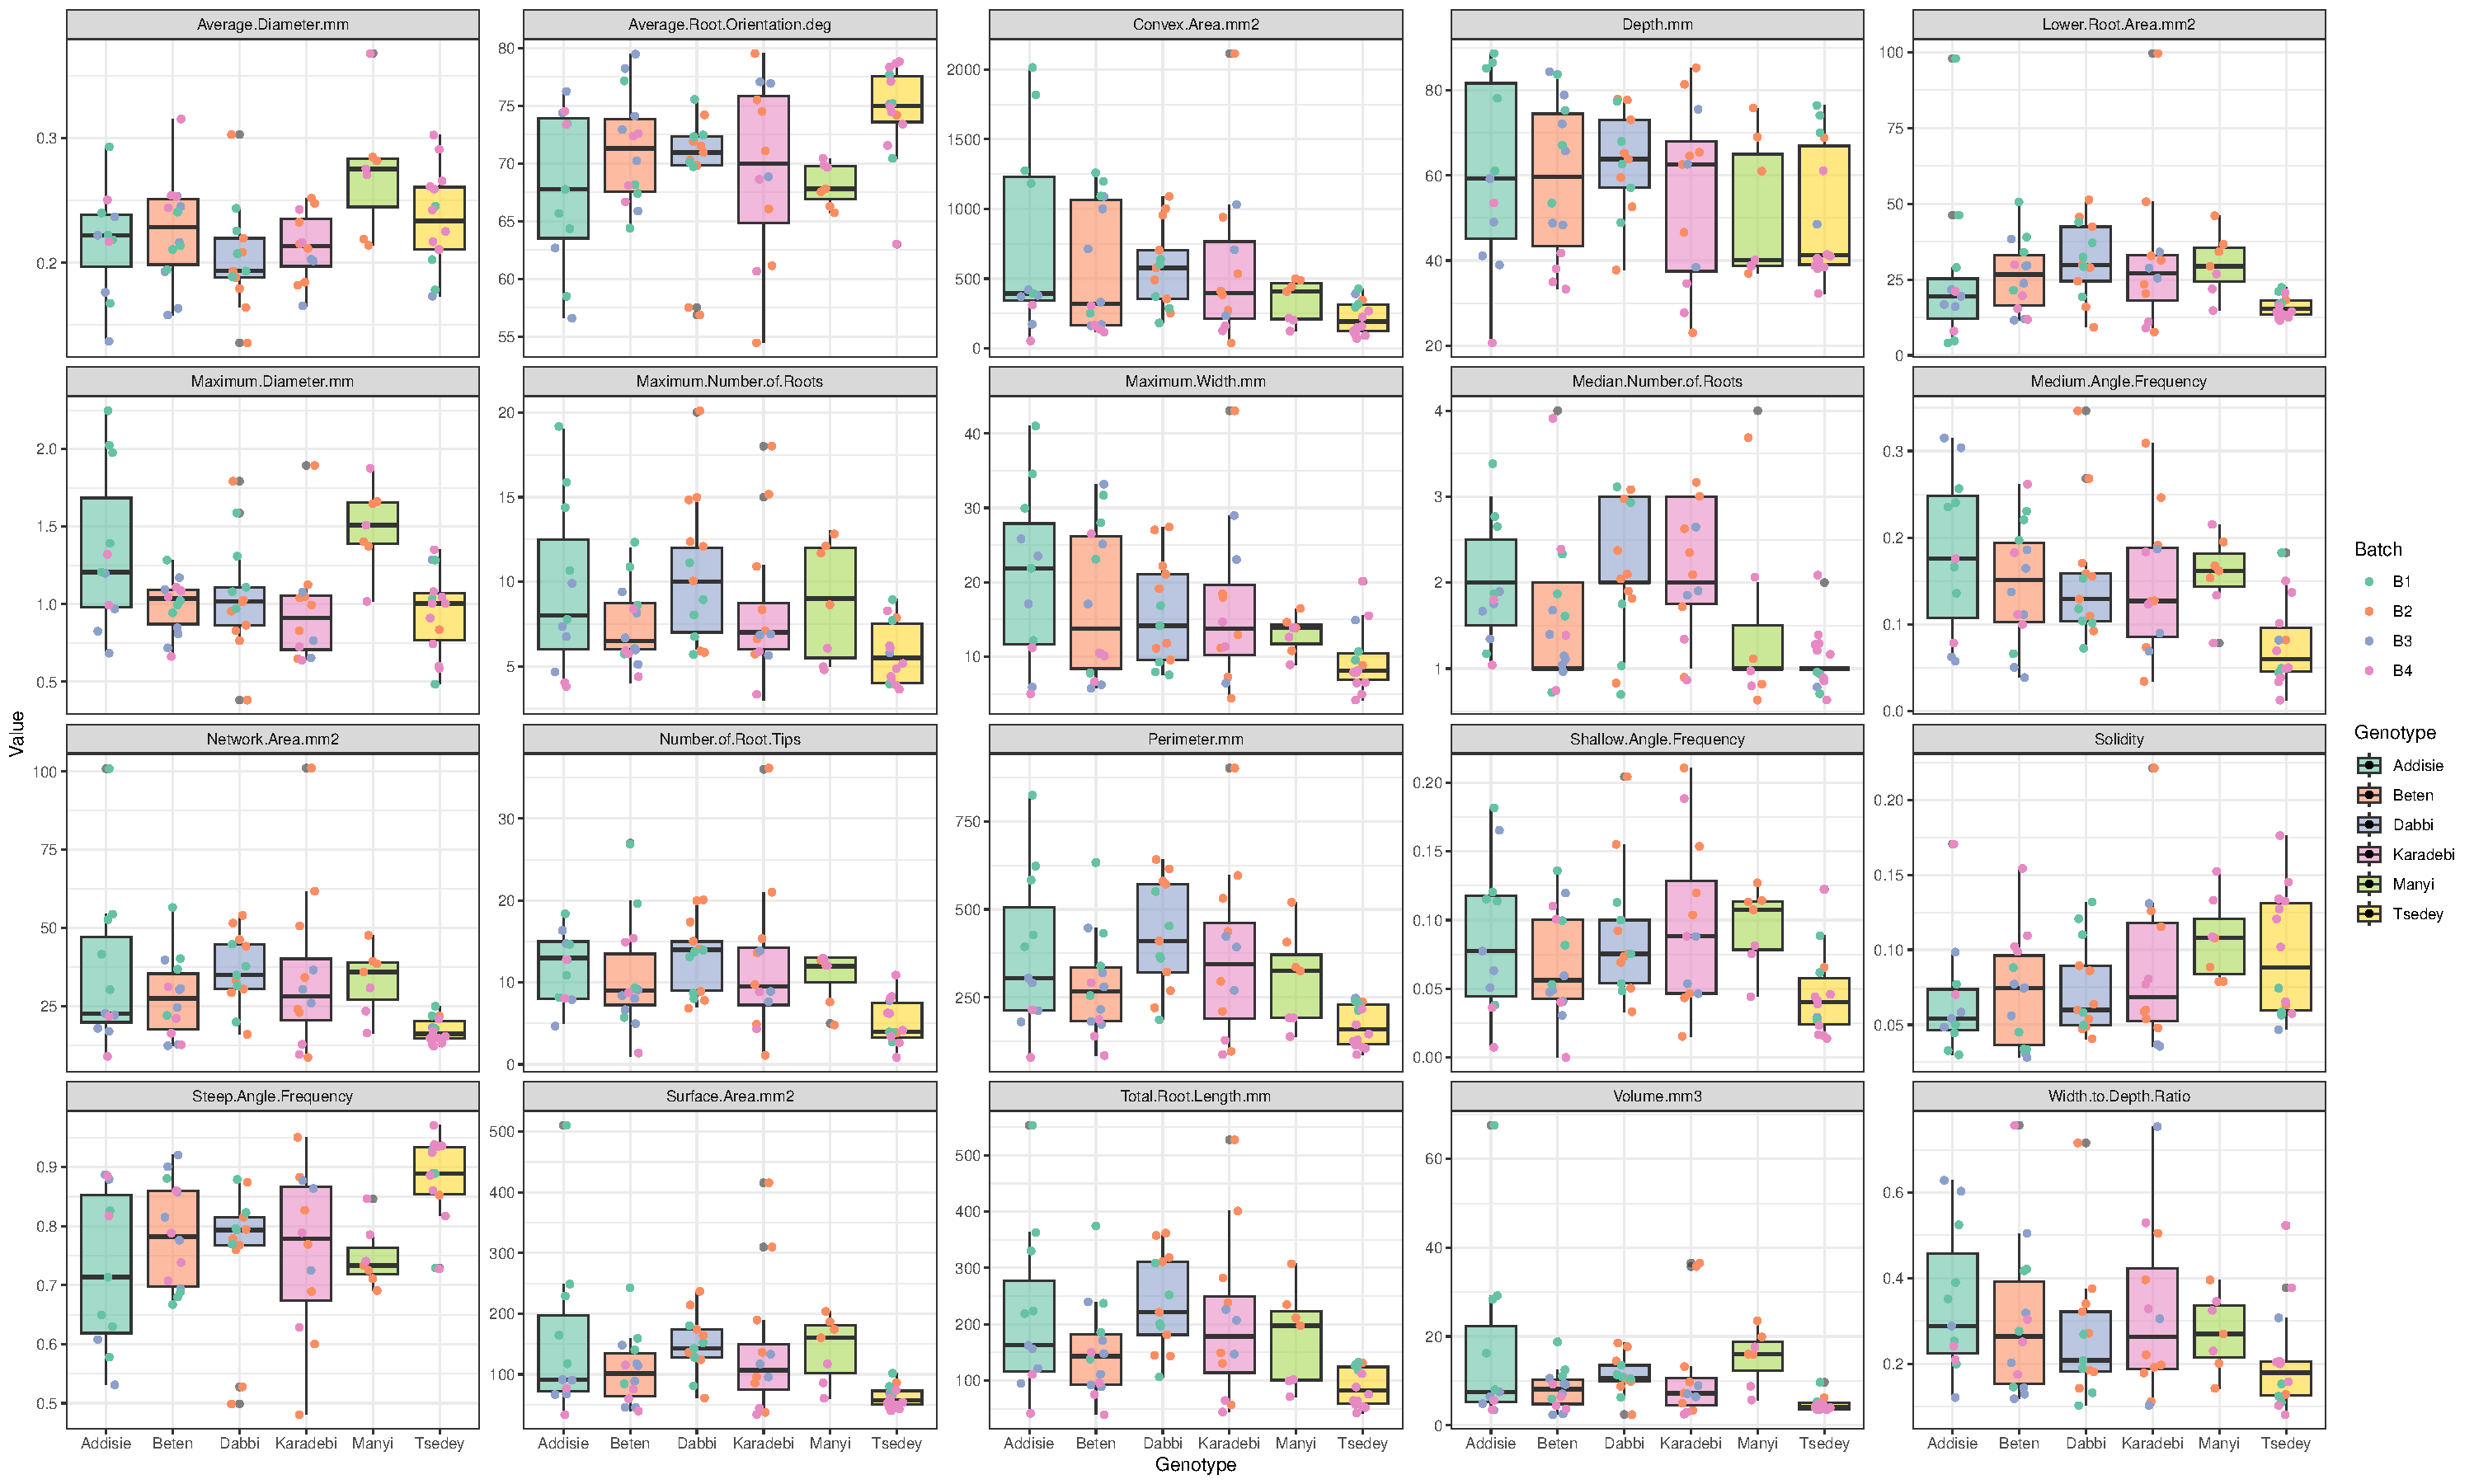
\includegraphics[keepaspectratio]{rsa_day1617_agar_files/figure-pdf/unnamed-chunk-2-1.pdf}}

Overall, box plot suggests broadly simlar phenotypes across the species
so will pick out individual traits to see if any significant differences
do arise.

\subsubsection{Number of Root Tips}\label{number-of-root-tips}

Assessing each factor individually

\begin{itemize}
\item
  Assess type of data
\item
  Decide best model
\item
  Check assumptions
\item
  Stats tests
\item
  Plots
\end{itemize}

\begin{Shaded}
\begin{Highlighting}[]
\CommentTok{\# ============================================================}
\CommentTok{\#  Number of Root Tips Analysis}
\CommentTok{\# ============================================================}

\CommentTok{\# ── 1. Inspect distribution ───────────────────────────────────}
\CommentTok{\# Root tips is a non{-}negative integer count — must use a count}
\CommentTok{\# distribution (Poisson or NB), not Gaussian.}
\FunctionTok{summary}\NormalTok{(df}\SpecialCharTok{$}\NormalTok{Number.of.Root.Tips)}
\end{Highlighting}
\end{Shaded}

\begin{verbatim}
   Min. 1st Qu.  Median    Mean 3rd Qu.    Max. 
   1.00    6.50    9.00   10.44   14.00   36.00 
\end{verbatim}

\begin{Shaded}
\begin{Highlighting}[]
\FunctionTok{cat}\NormalTok{(}\StringTok{"Var/Mean ratio:"}\NormalTok{, }\FunctionTok{round}\NormalTok{(}\FunctionTok{var}\NormalTok{(df}\SpecialCharTok{$}\NormalTok{Number.of.Root.Tips) }\SpecialCharTok{/}
      \FunctionTok{mean}\NormalTok{(df}\SpecialCharTok{$}\NormalTok{Number.of.Root.Tips), }\DecValTok{3}\NormalTok{),}
    \StringTok{"(\textgreater{}1 suggests overdispersion)}\SpecialCharTok{\textbackslash{}n}\StringTok{"}\NormalTok{)}
\end{Highlighting}
\end{Shaded}

\begin{verbatim}
Var/Mean ratio: 3.569 (>1 suggests overdispersion)
\end{verbatim}

\begin{Shaded}
\begin{Highlighting}[]
\CommentTok{\# Histogram to visualise shape and identify skew or zero{-}inflation}
\FunctionTok{ggplot}\NormalTok{(df, }\FunctionTok{aes}\NormalTok{(}\AttributeTok{x =}\NormalTok{ Number.of.Root.Tips)) }\SpecialCharTok{+}
  \FunctionTok{geom\_histogram}\NormalTok{(}\AttributeTok{binwidth =} \DecValTok{3}\NormalTok{, }\AttributeTok{fill =} \StringTok{"\#66C2A5"}\NormalTok{, }\AttributeTok{colour =} \StringTok{"white"}\NormalTok{) }\SpecialCharTok{+}
  \FunctionTok{geom\_vline}\NormalTok{(}\AttributeTok{xintercept =} \FunctionTok{mean}\NormalTok{(df}\SpecialCharTok{$}\NormalTok{Number.of.Root.Tips),}
             \AttributeTok{linetype =} \StringTok{"dashed"}\NormalTok{, }\AttributeTok{colour =} \StringTok{"red"}\NormalTok{) }\SpecialCharTok{+}
  \FunctionTok{labs}\NormalTok{(}\AttributeTok{x =} \StringTok{"Number of root tips"}\NormalTok{, }\AttributeTok{y =} \StringTok{"Count"}\NormalTok{) }\SpecialCharTok{+}
  \FunctionTok{theme\_classic}\NormalTok{(}\AttributeTok{base\_size =} \DecValTok{14}\NormalTok{)}
\end{Highlighting}
\end{Shaded}

\pandocbounded{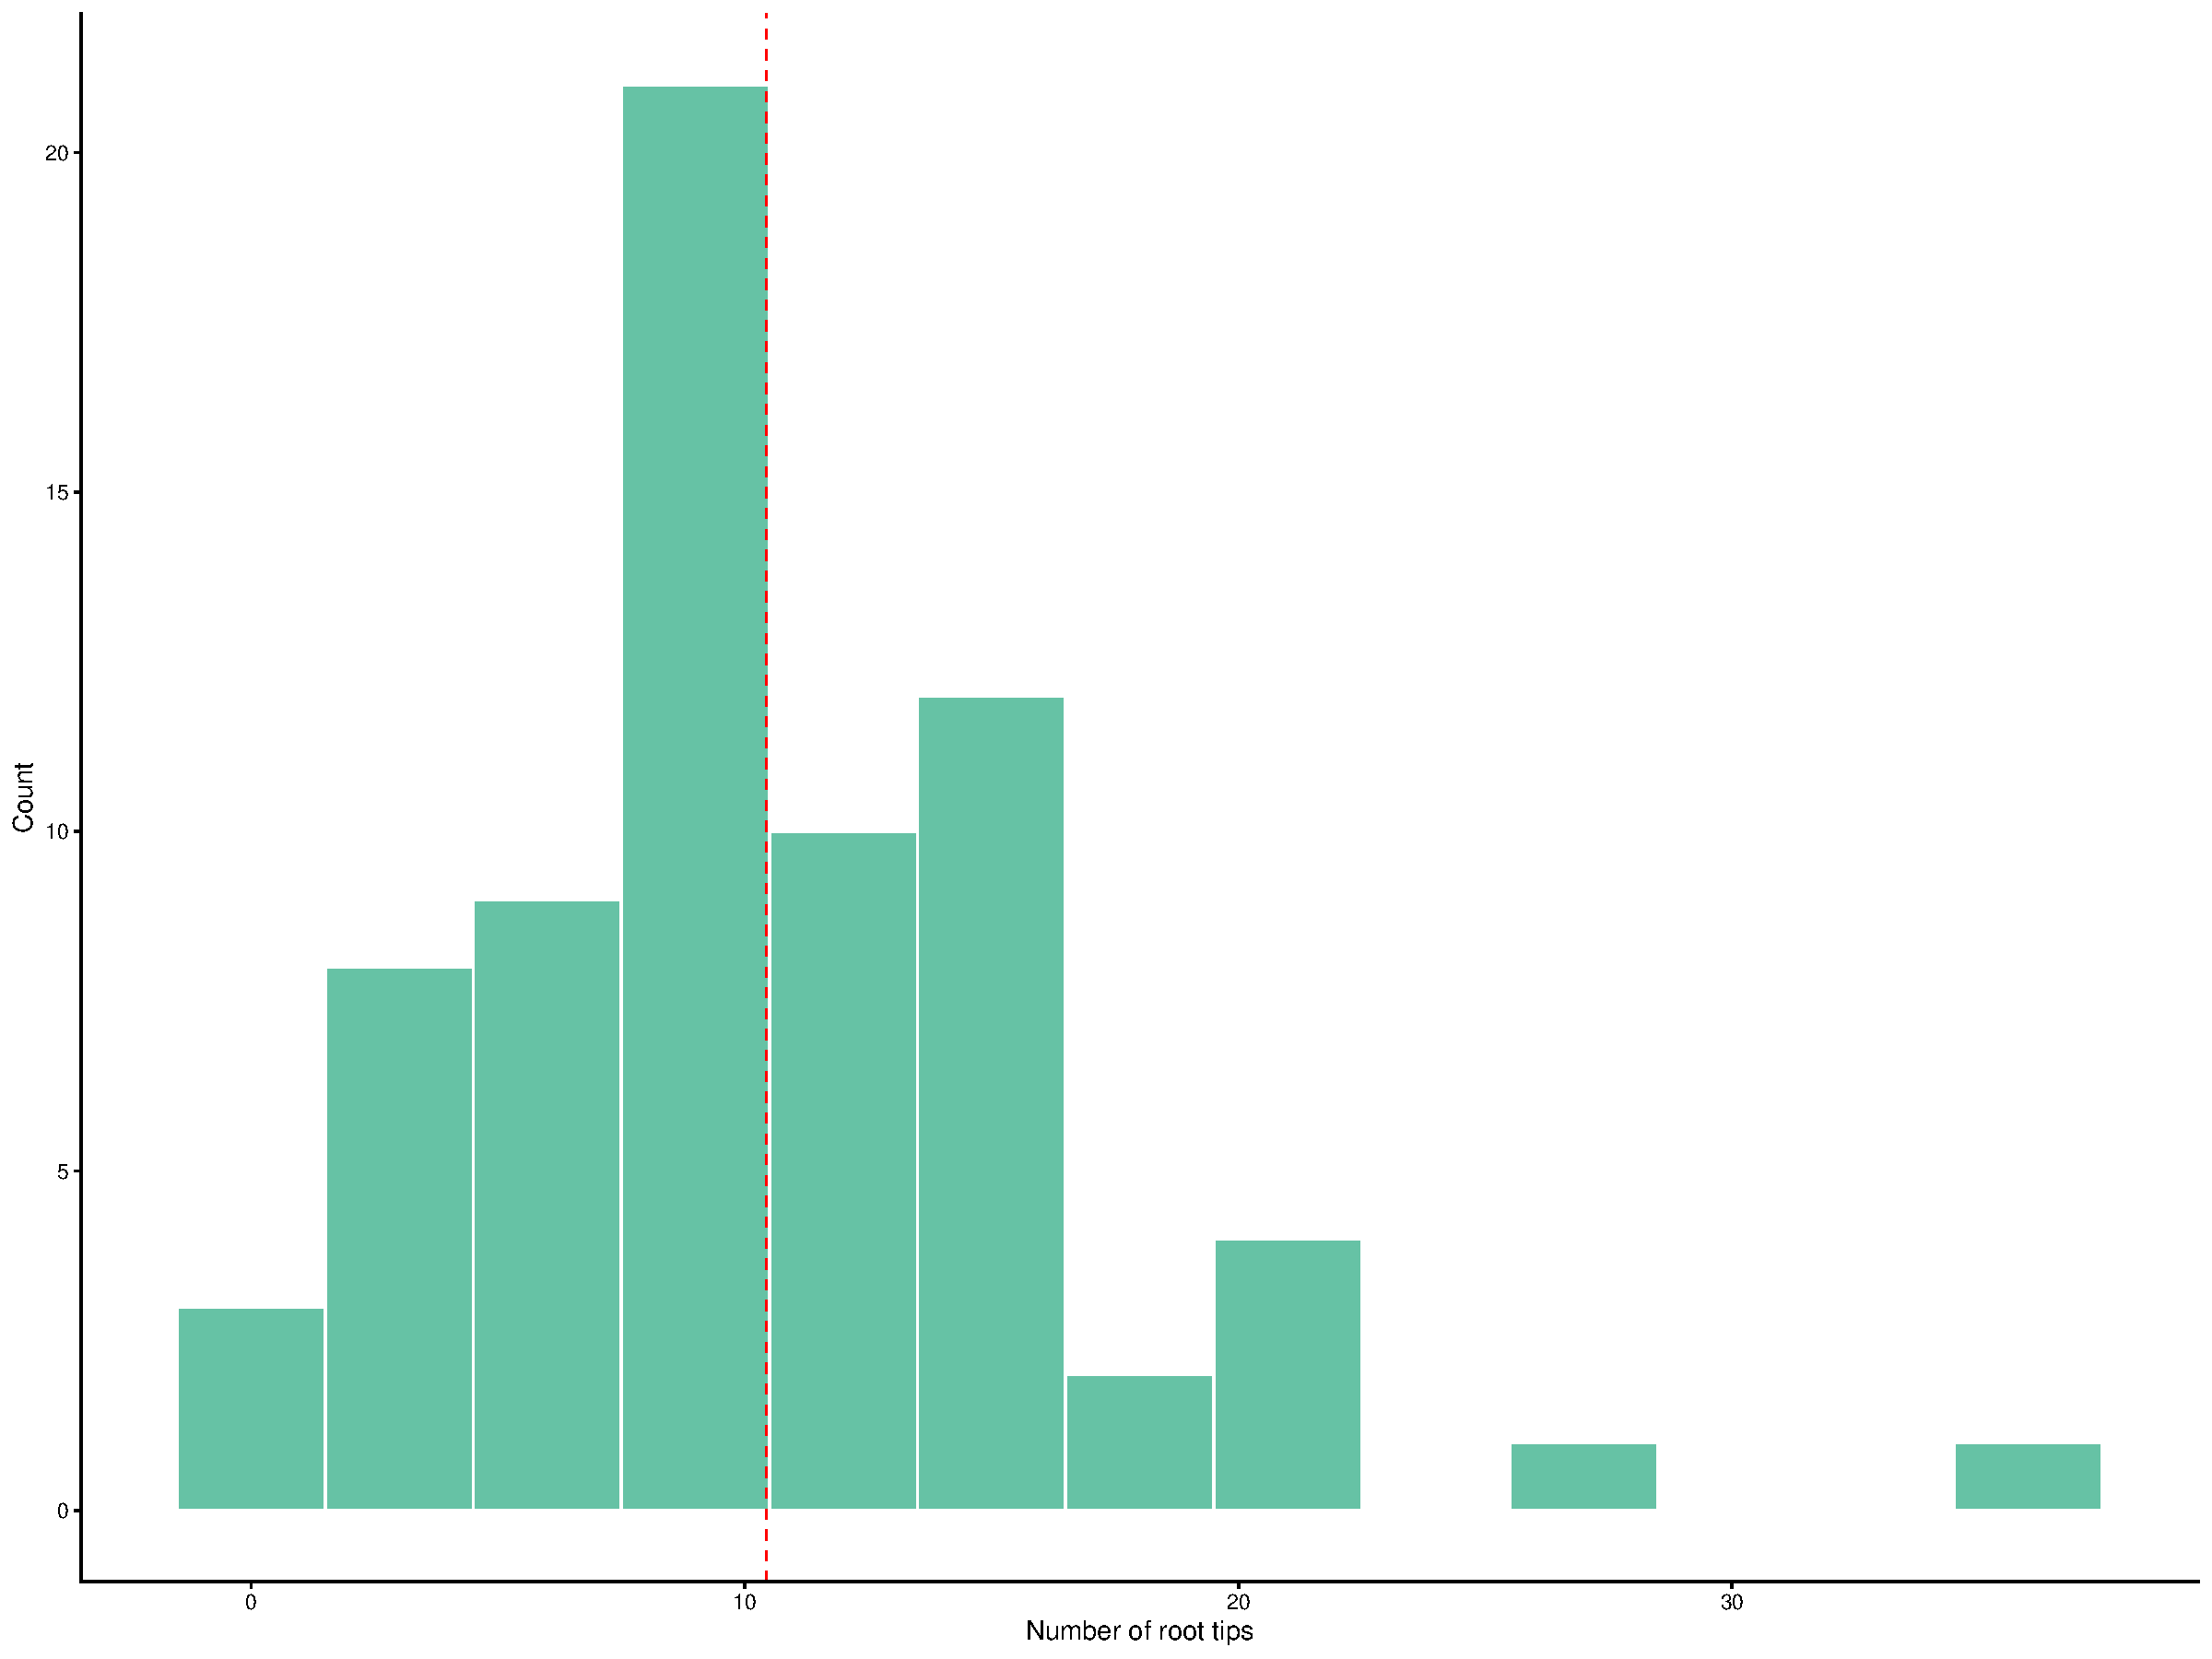
\includegraphics[keepaspectratio]{rsa_day1617_agar_files/figure-pdf/unnamed-chunk-3-1.pdf}}

\begin{Shaded}
\begin{Highlighting}[]
\CommentTok{\# ── 2. Fit Poisson to formally confirm overdispersion ─────────}
\CommentTok{\# We fit Poisson first to formally test whether its assumption}
\CommentTok{\# (variance = mean) holds. If DHARMa flags overdispersion}
\CommentTok{\# (p \textless{} 0.05, ratio \textgreater{}\textgreater{} 1), we reject Poisson and move to NB.}
\CommentTok{\# Random effects: seeds nested in plates nested in batches —}
\CommentTok{\# ignoring this clustering would pseudoreplicate as plants on}
\CommentTok{\# the same plate share physical and nutritional environment.}
\NormalTok{tips\_tmb\_pois }\OtherTok{\textless{}{-}} \FunctionTok{glmmTMB}\NormalTok{(}
\NormalTok{  Number.of.Root.Tips }\SpecialCharTok{\textasciitilde{}}\NormalTok{ Genotype }\SpecialCharTok{+}\NormalTok{ (}\DecValTok{1} \SpecialCharTok{|}\NormalTok{ Batch}\SpecialCharTok{/}\NormalTok{Plate}\SpecialCharTok{/}\NormalTok{Seed),}
  \AttributeTok{data =}\NormalTok{ df, }\AttributeTok{family =}\NormalTok{ poisson}
\NormalTok{)}

\NormalTok{sim\_pois }\OtherTok{\textless{}{-}} \FunctionTok{simulateResiduals}\NormalTok{(tips\_tmb\_pois, }\AttributeTok{n =} \DecValTok{1000}\NormalTok{)}
\FunctionTok{plot}\NormalTok{(sim\_pois)}
\end{Highlighting}
\end{Shaded}

\pandocbounded{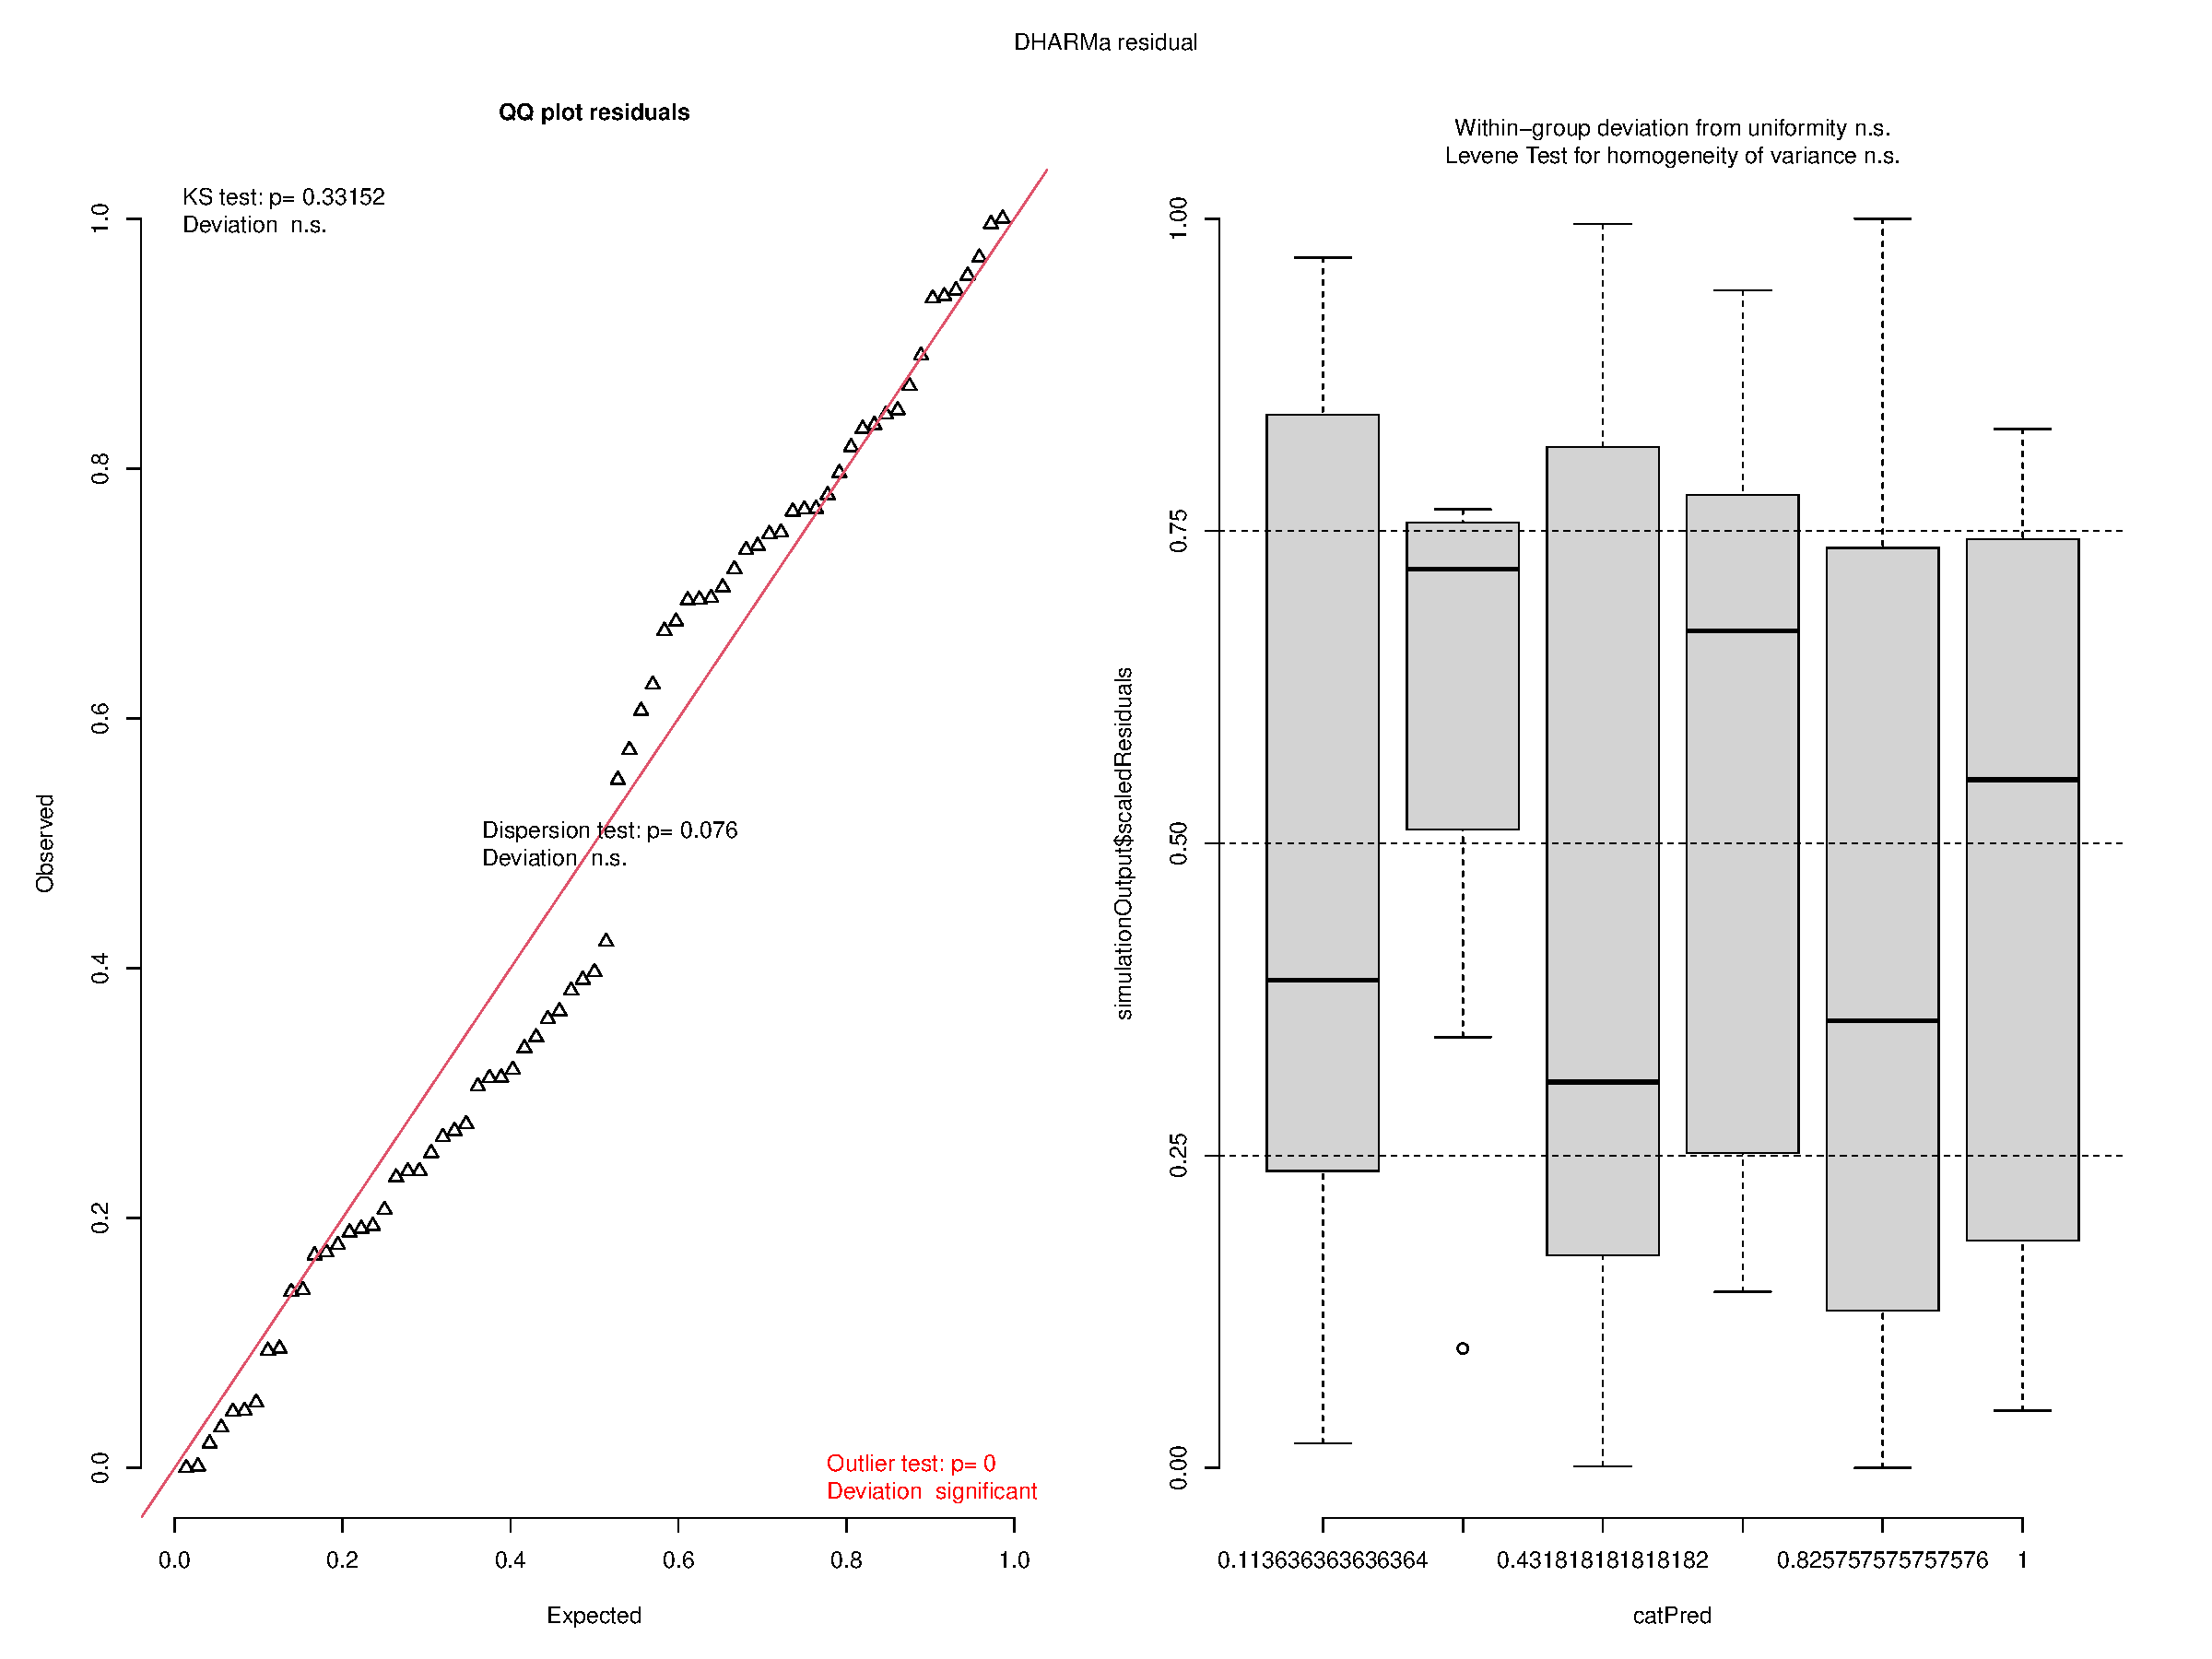
\includegraphics[keepaspectratio]{rsa_day1617_agar_files/figure-pdf/unnamed-chunk-3-2.pdf}}

\begin{Shaded}
\begin{Highlighting}[]
\FunctionTok{testDispersion}\NormalTok{(sim\_pois)   }\CommentTok{\# p \textless{} 0.05 → overdispersed → try NB to see if there is a better fit}
\end{Highlighting}
\end{Shaded}

\pandocbounded{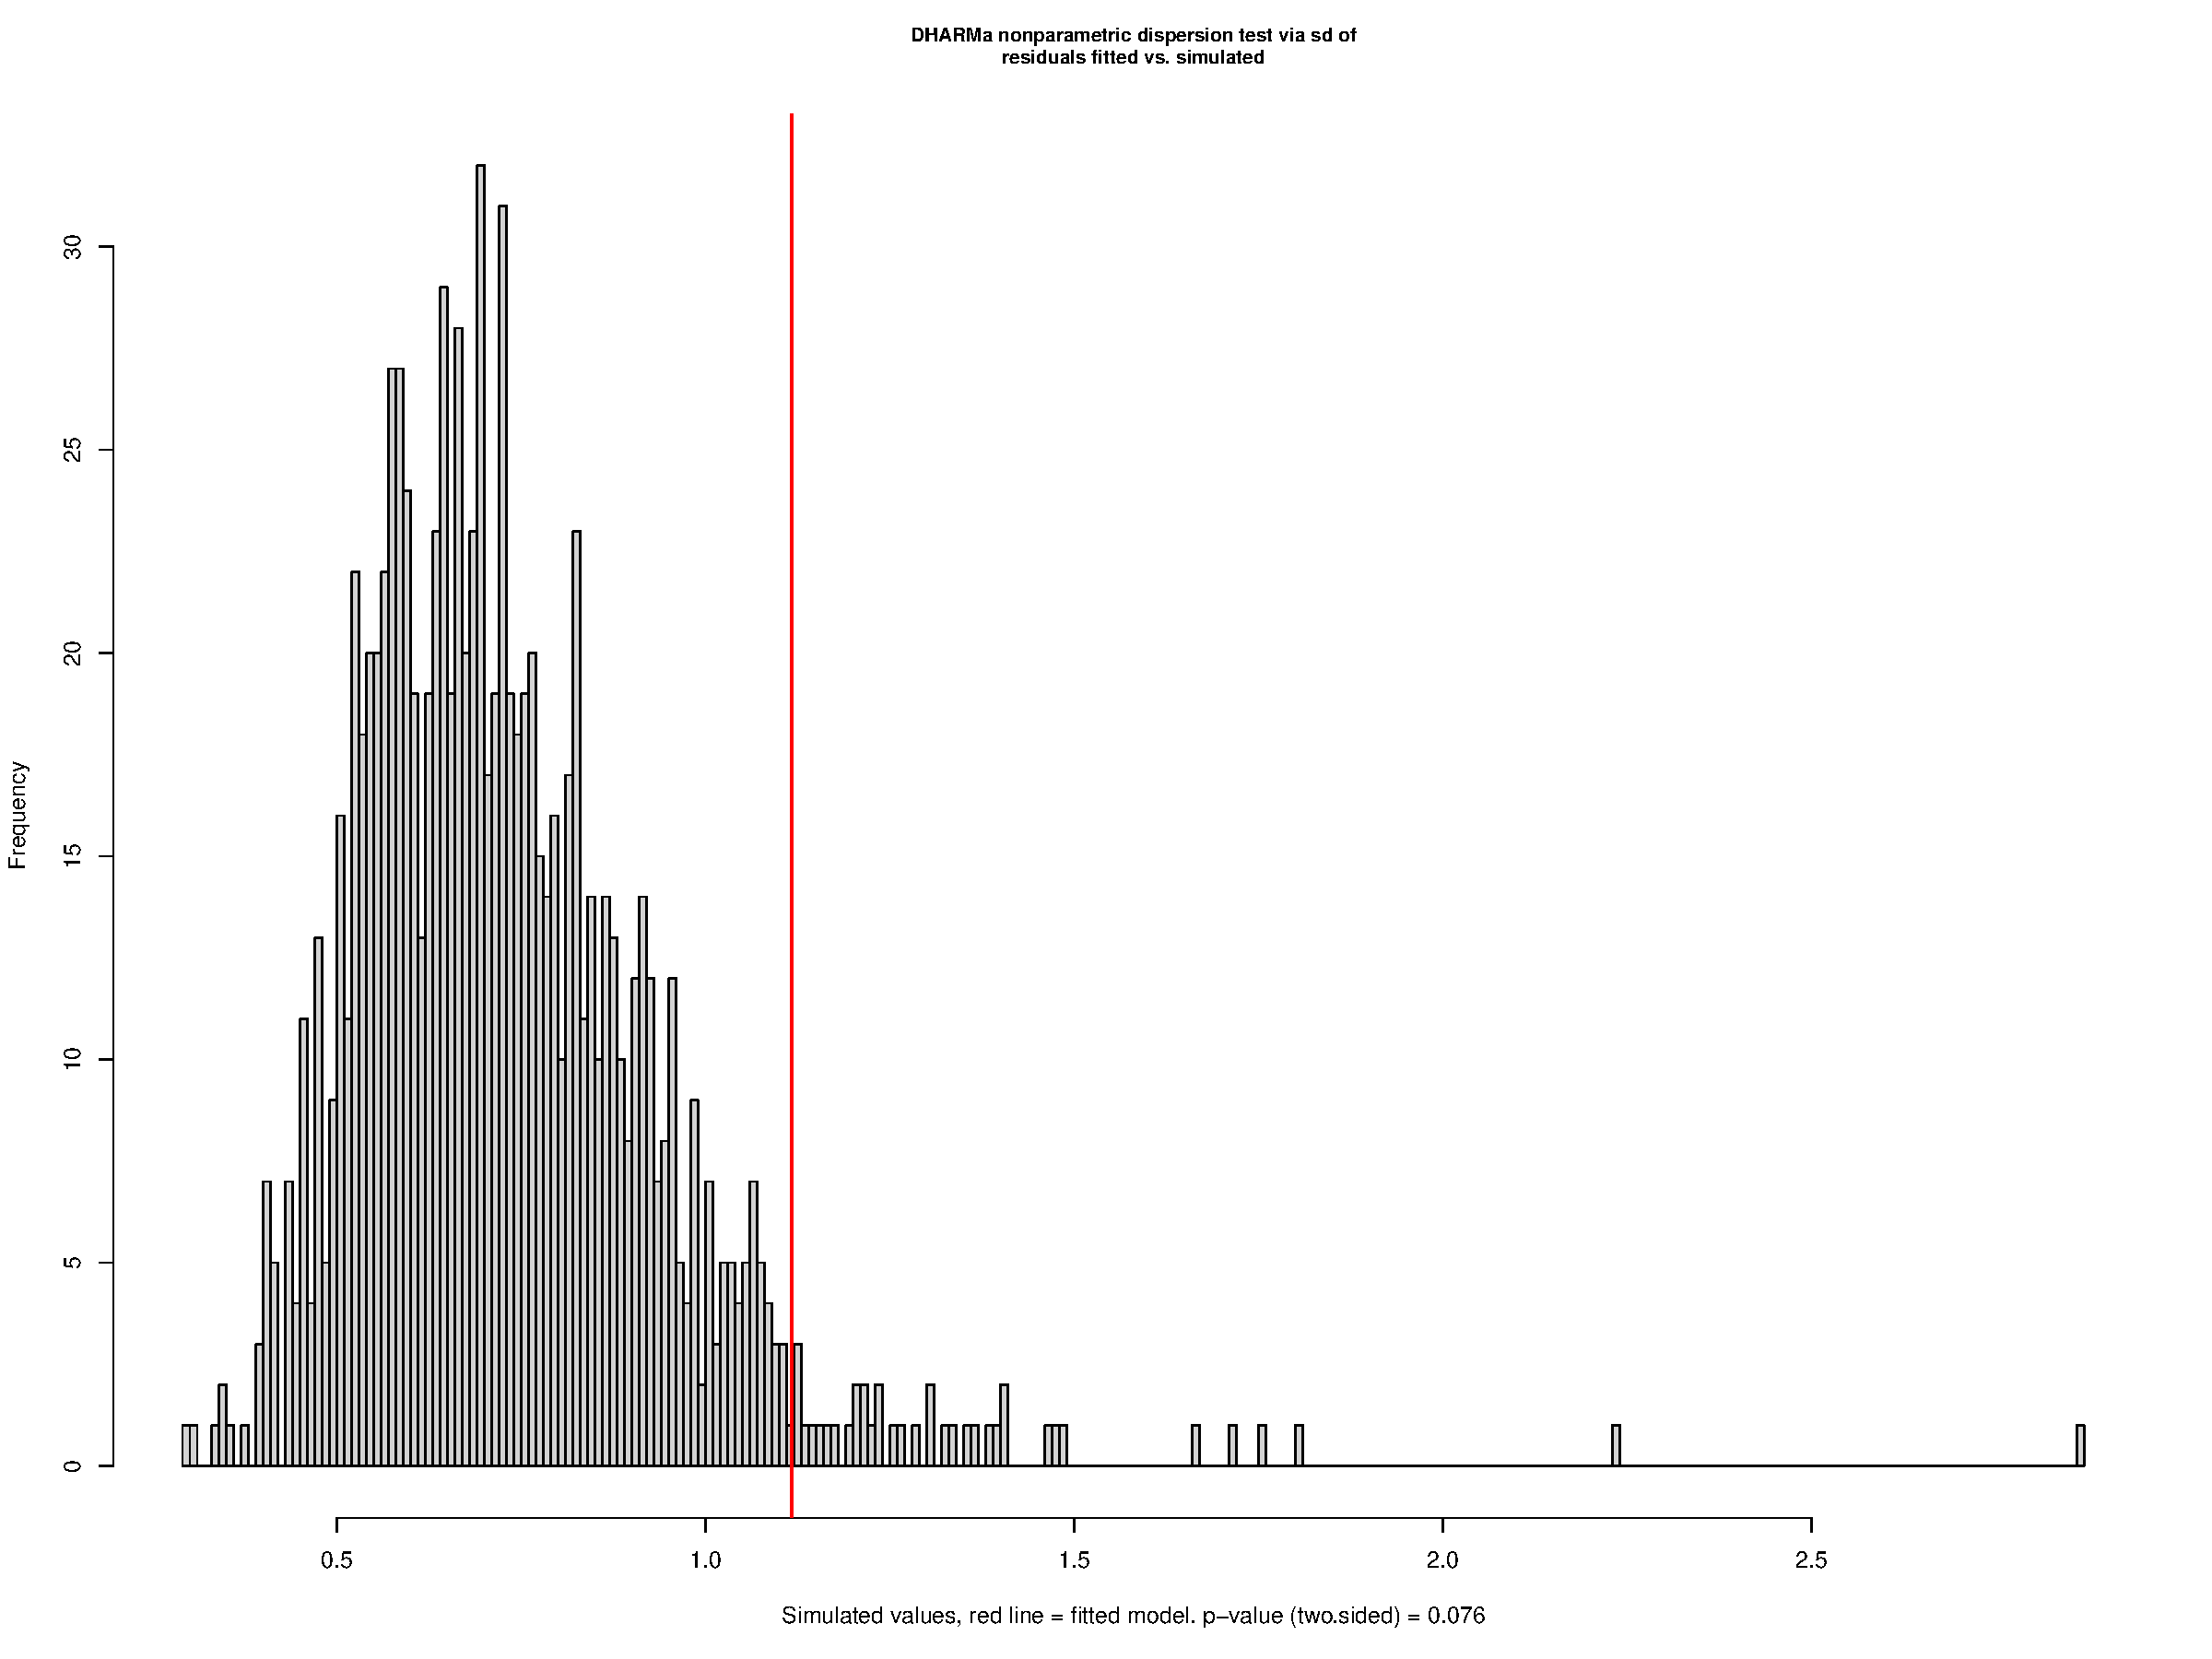
\includegraphics[keepaspectratio]{rsa_day1617_agar_files/figure-pdf/unnamed-chunk-3-3.pdf}}

\begin{verbatim}

    DHARMa nonparametric dispersion test via sd of residuals fitted vs.
    simulated

data:  simulationOutput
dispersion = 1.5236, p-value = 0.076
alternative hypothesis: two.sided
\end{verbatim}

\begin{Shaded}
\begin{Highlighting}[]
\CommentTok{\# the residual plots show from outlier test the deviation is significant so we will try NB}

\CommentTok{\# ── 3. Compare nb2 vs nb1 ─────────────────────────────────────}
\CommentTok{\# Two NB parameterisations:}
\CommentTok{\#   nb2: variance = mu + mu²/theta — quadratic, most common for}
\CommentTok{\#        biological count data where variance scales with mean²}
\CommentTok{\#   nb1: variance = phi*mu — linear, less common}
\CommentTok{\# Select using AIC (lower = better) and DHARMa visual diagnostics.}

\NormalTok{tips\_tmb\_nb2 }\OtherTok{\textless{}{-}} \FunctionTok{glmmTMB}\NormalTok{(}
\NormalTok{  Number.of.Root.Tips }\SpecialCharTok{\textasciitilde{}}\NormalTok{ Genotype }\SpecialCharTok{+}\NormalTok{ (}\DecValTok{1} \SpecialCharTok{|}\NormalTok{ Batch}\SpecialCharTok{/}\NormalTok{Plate}\SpecialCharTok{/}\NormalTok{Seed),}
  \AttributeTok{data =}\NormalTok{ df, }\AttributeTok{family =}\NormalTok{ nbinom2}
\NormalTok{)}

\NormalTok{tips\_tmb\_nb1 }\OtherTok{\textless{}{-}} \FunctionTok{glmmTMB}\NormalTok{(}
\NormalTok{  Number.of.Root.Tips }\SpecialCharTok{\textasciitilde{}}\NormalTok{ Genotype }\SpecialCharTok{+}\NormalTok{ (}\DecValTok{1} \SpecialCharTok{|}\NormalTok{ Batch}\SpecialCharTok{/}\NormalTok{Plate}\SpecialCharTok{/}\NormalTok{Seed),}
  \AttributeTok{data =}\NormalTok{ df, }\AttributeTok{family =}\NormalTok{ nbinom1}
\NormalTok{)}
\end{Highlighting}
\end{Shaded}

\begin{verbatim}
Warning in finalizeTMB(TMBStruc, obj, fit, h, data.tmb.old): Model convergence
problem; non-positive-definite Hessian matrix. See vignette('troubleshooting')
\end{verbatim}

\begin{Shaded}
\begin{Highlighting}[]
\CommentTok{\# AIC comparison — lower = better fit penalised for complexity}
\FunctionTok{AIC}\NormalTok{(tips\_tmb\_pois, tips\_tmb\_nb1, tips\_tmb\_nb2)}
\end{Highlighting}
\end{Shaded}

\begin{verbatim}
              df      AIC
tips_tmb_pois  9 462.4599
tips_tmb_nb1  10       NA
tips_tmb_nb2  10 441.3074
\end{verbatim}

\begin{Shaded}
\begin{Highlighting}[]
\CommentTok{\# find that NB2 is better than poisson and NB1 fails so will continue with NB2}

\CommentTok{\# DHARMa residuals for each NB model — choose the one with}
\CommentTok{\# better QQ alignment and flatter residual vs fitted panel}
\NormalTok{sim\_nb2 }\OtherTok{\textless{}{-}} \FunctionTok{simulateResiduals}\NormalTok{(tips\_tmb\_nb2, }\AttributeTok{n =} \DecValTok{1000}\NormalTok{)}
\FunctionTok{plot}\NormalTok{(sim\_nb2)}
\end{Highlighting}
\end{Shaded}

\pandocbounded{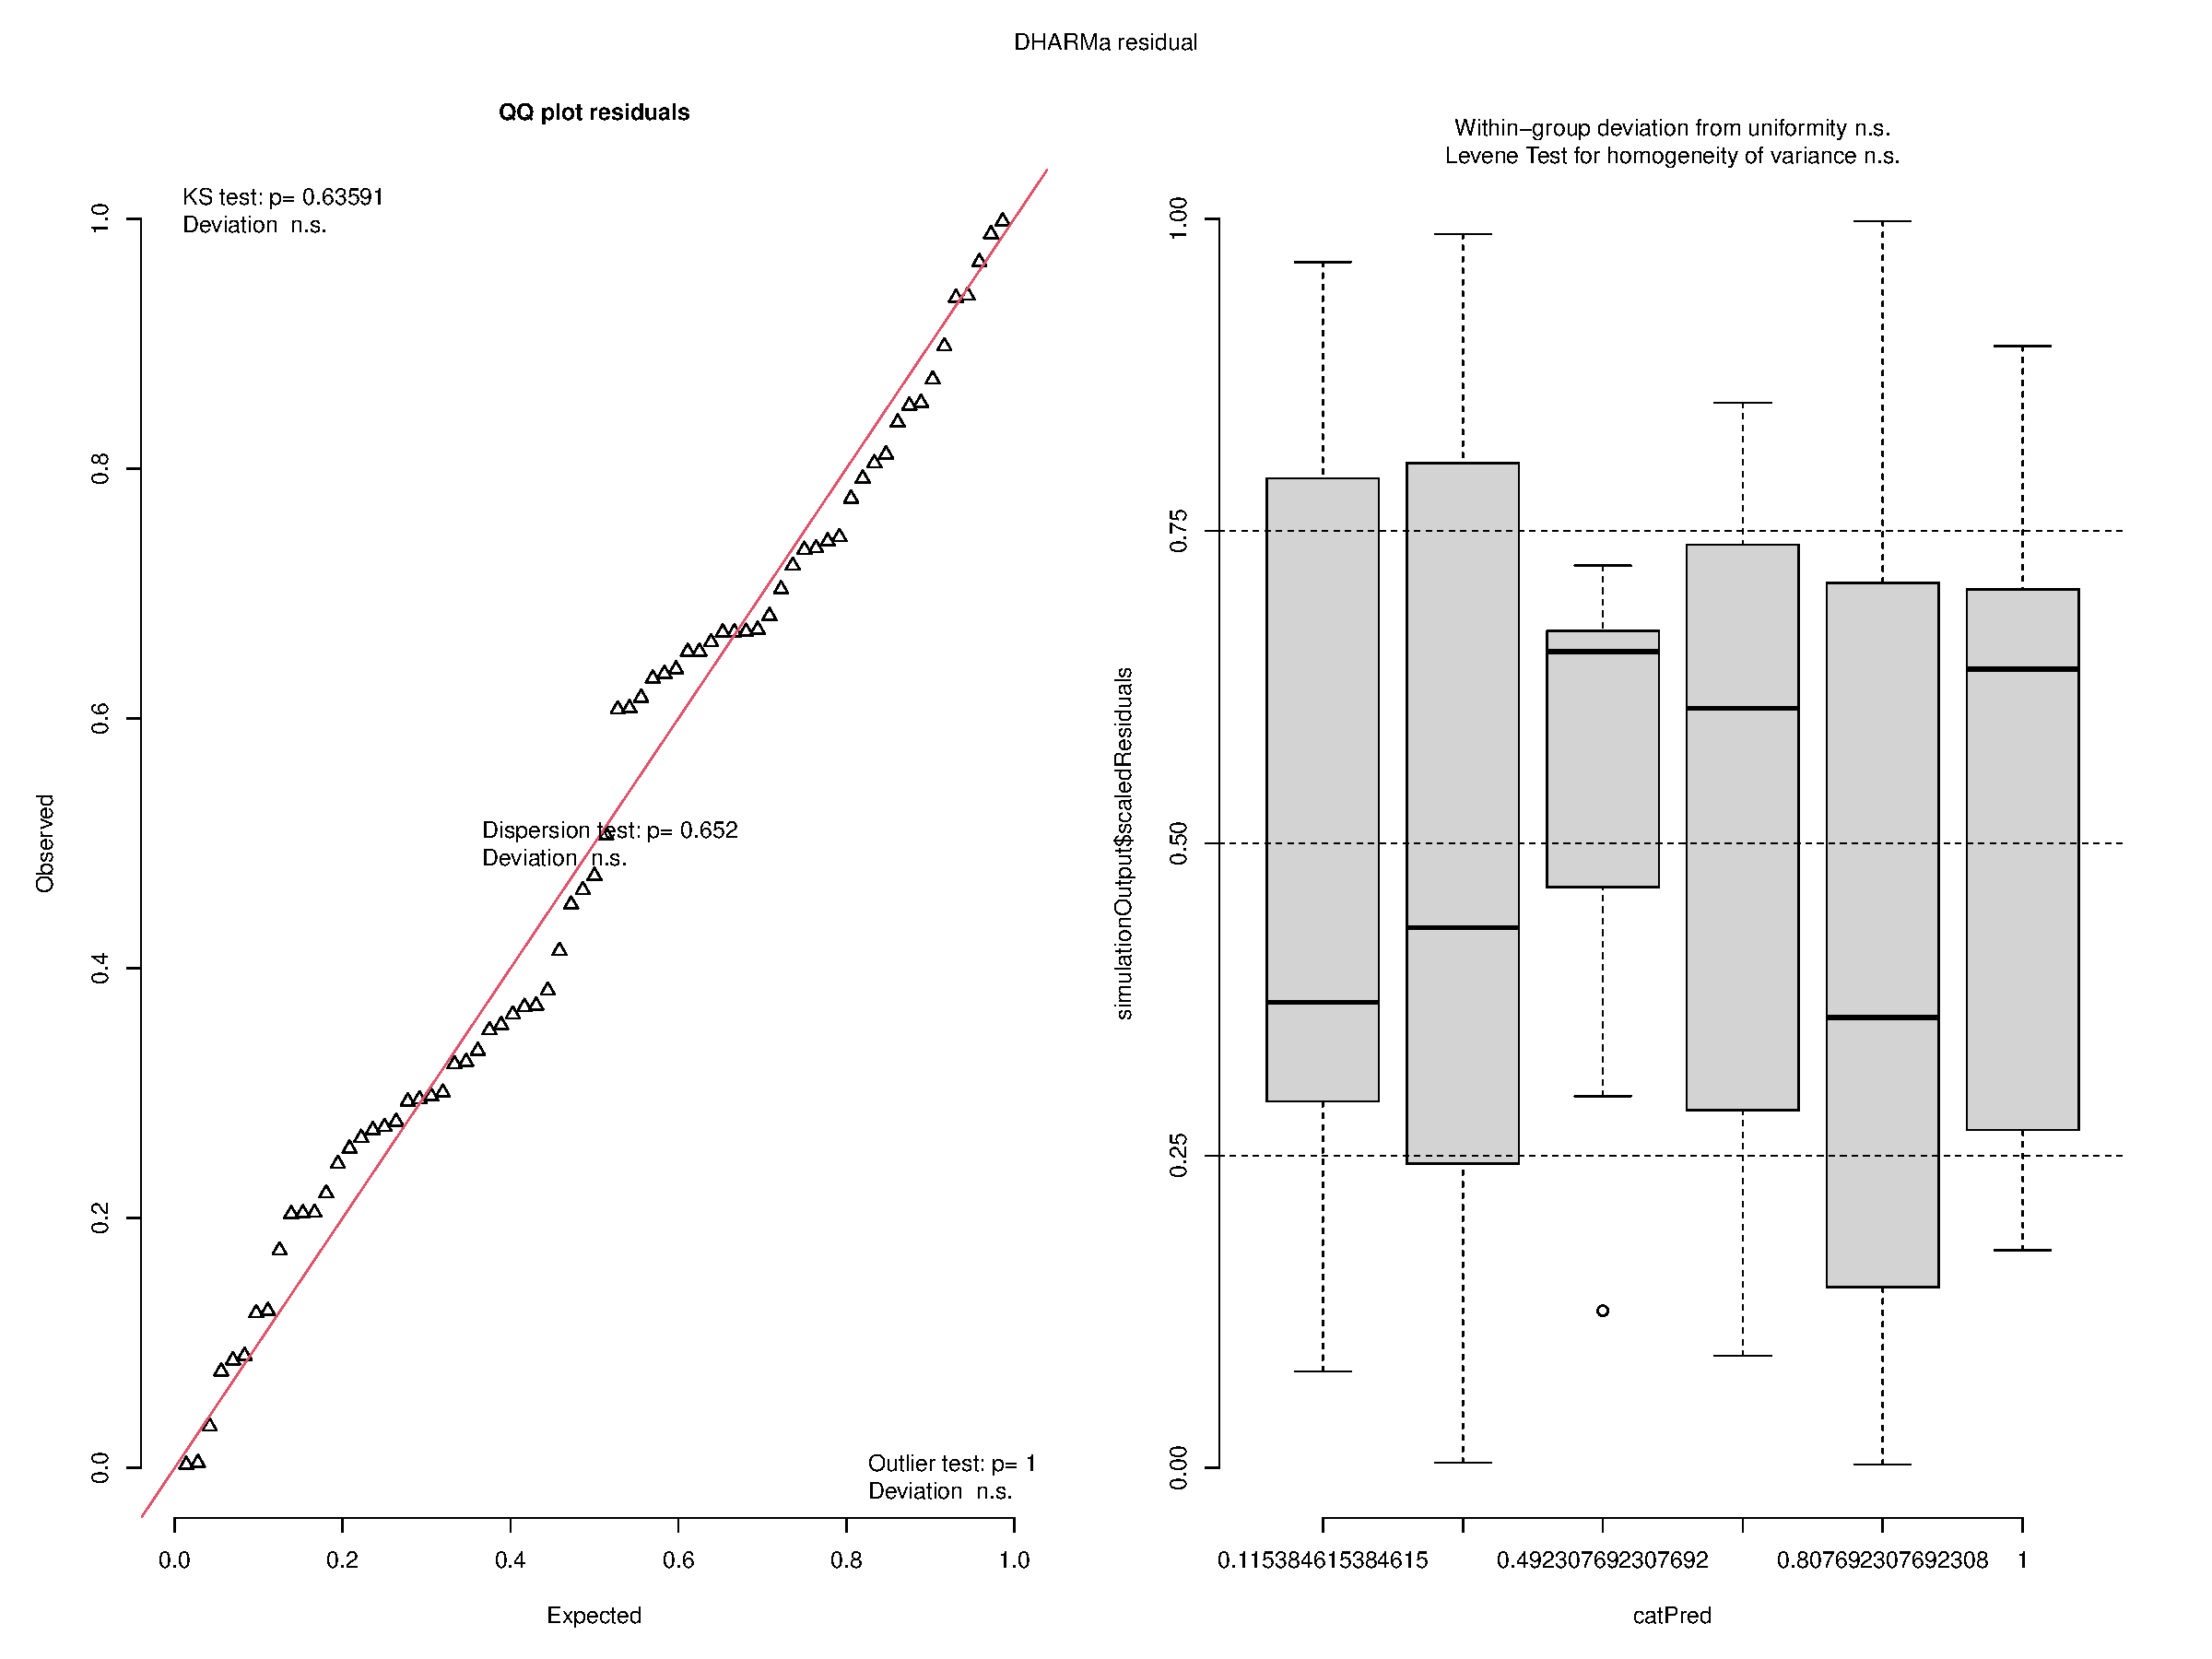
\includegraphics[keepaspectratio]{rsa_day1617_agar_files/figure-pdf/unnamed-chunk-3-4.pdf}}

\begin{Shaded}
\begin{Highlighting}[]
\CommentTok{\# ── 4. Full assumption checks on chosen model (nb2) ───────────}
\CommentTok{\# testUniformity: residuals should be uniformly distributed (p \textgreater{} 0.05)}
\CommentTok{\# testDispersion: ratio ≈ 1.0 confirms variance correctly specified}
\CommentTok{\# testZeroInflation: checks if zeros are over{-}represented beyond NB}
\CommentTok{\# testOutliers: flags any observations with extreme residuals}
\FunctionTok{testUniformity}\NormalTok{(sim\_nb2)}
\end{Highlighting}
\end{Shaded}

\pandocbounded{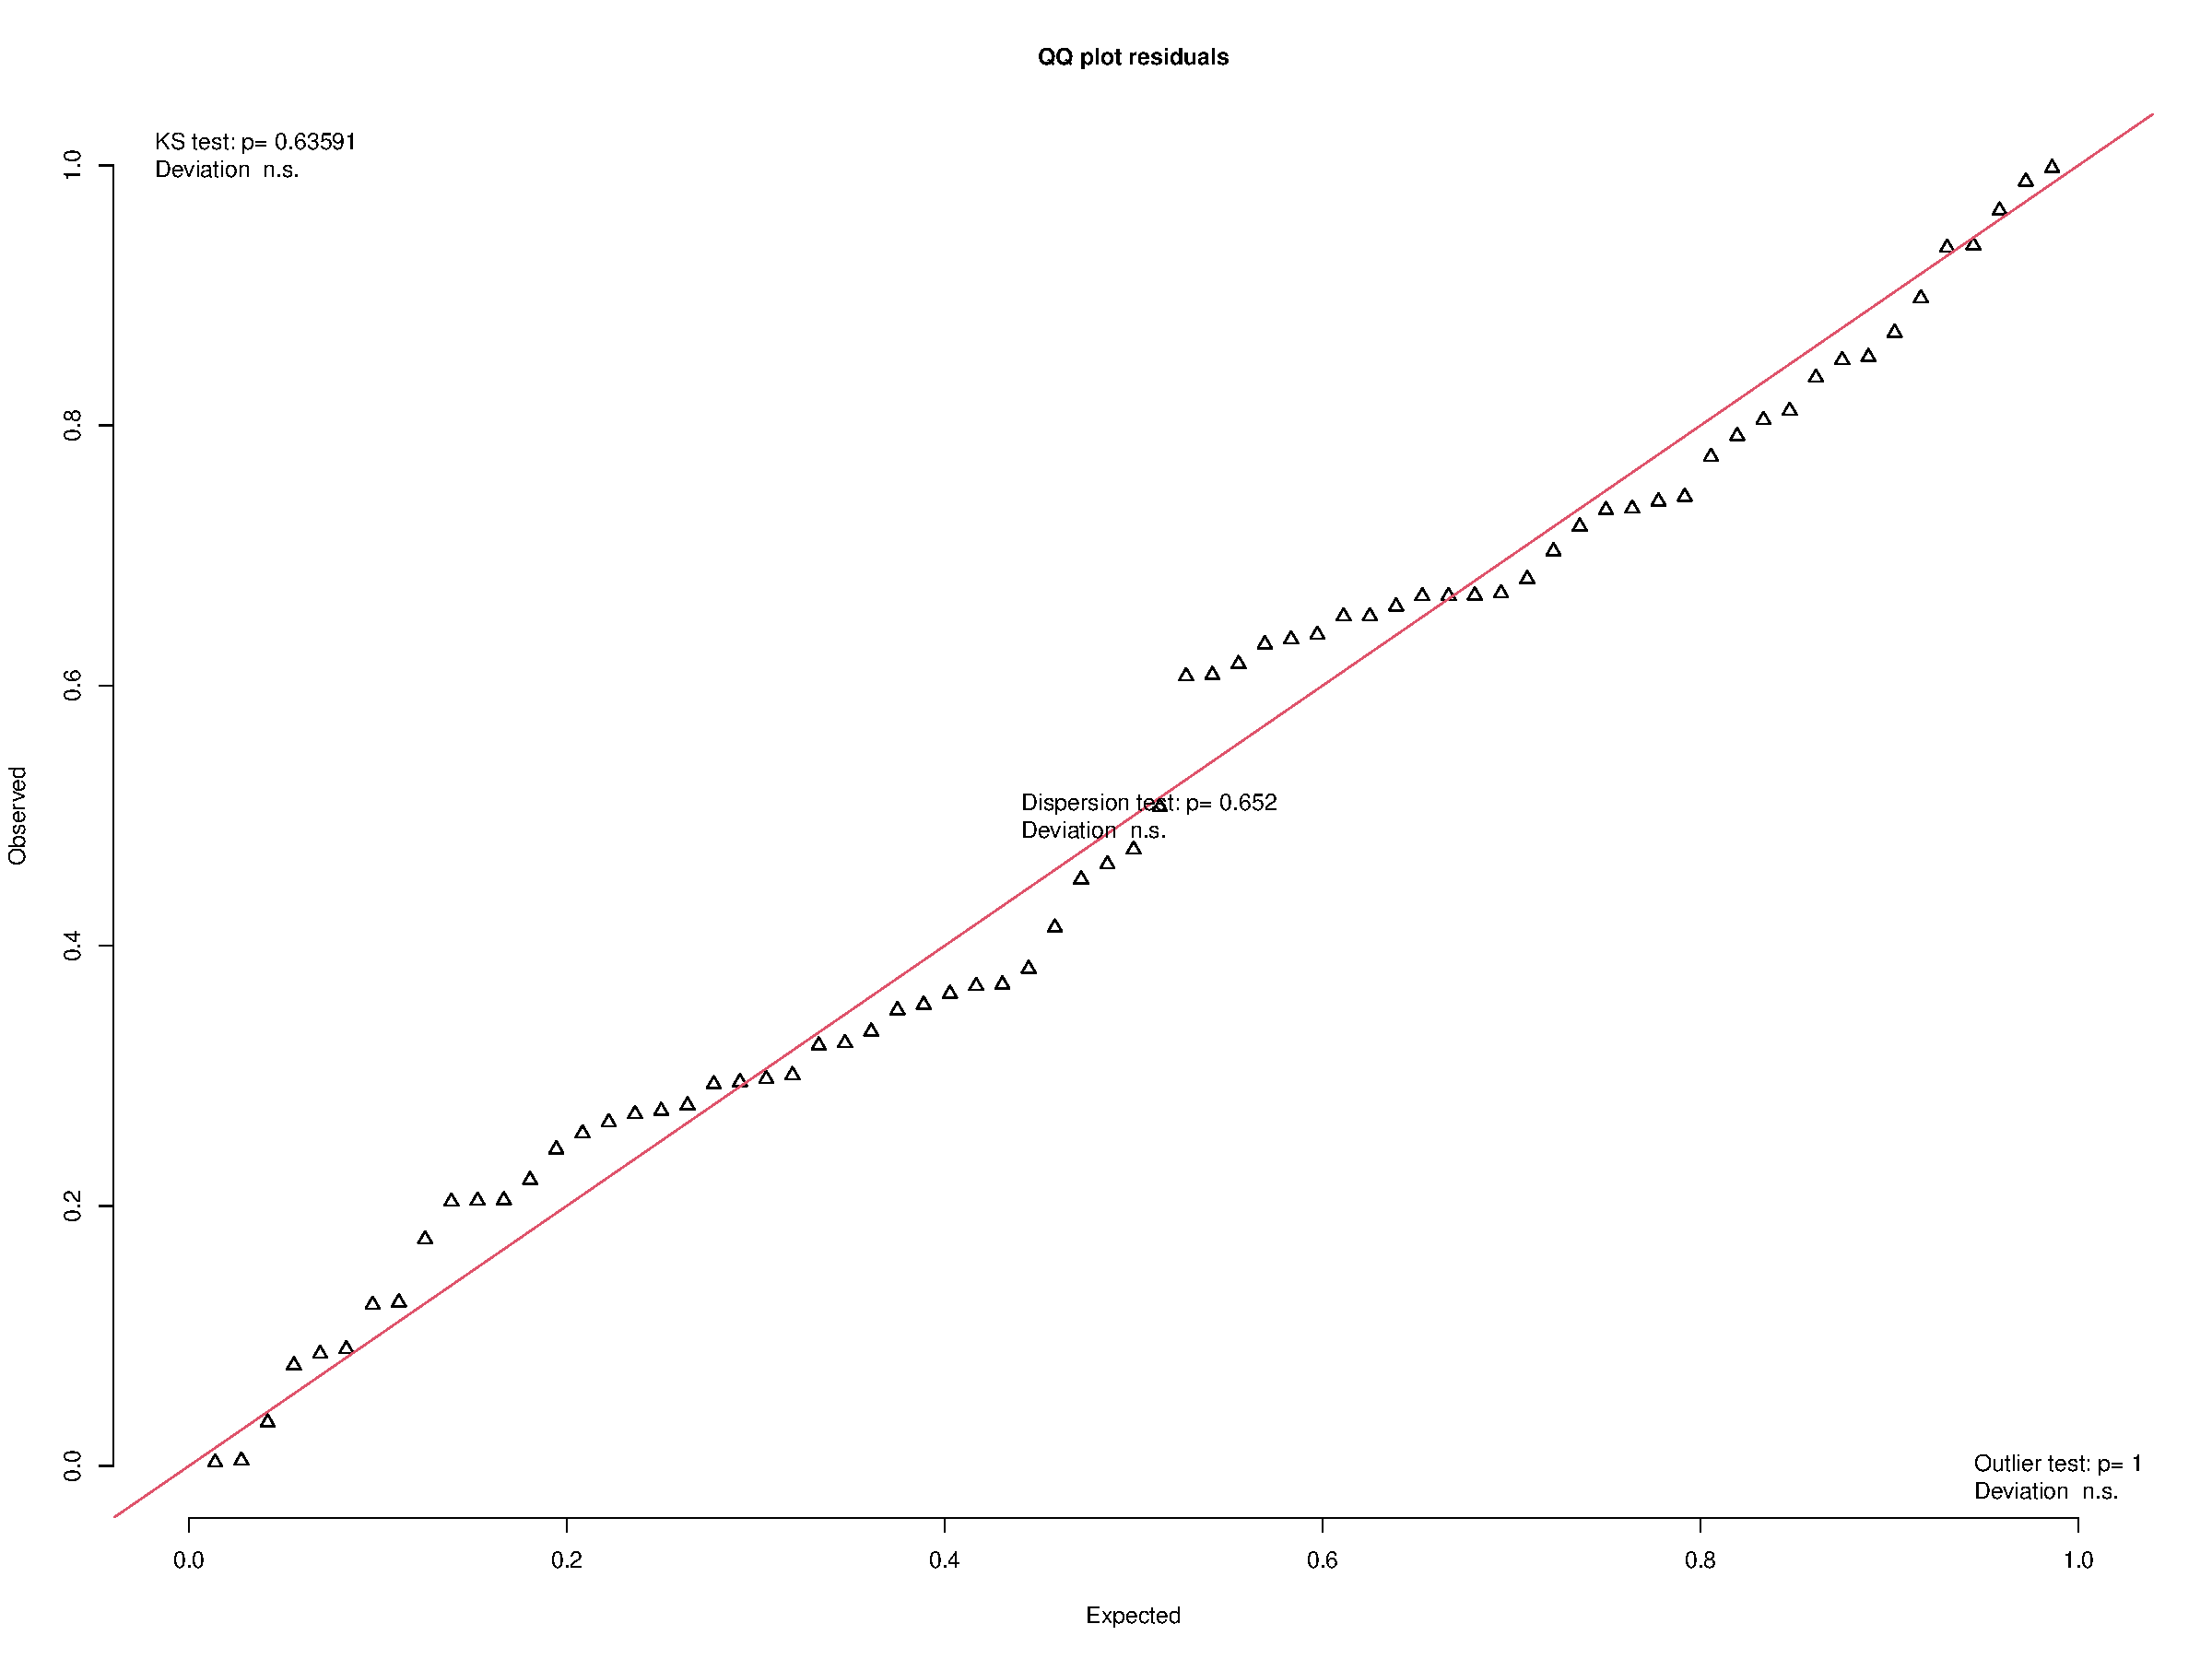
\includegraphics[keepaspectratio]{rsa_day1617_agar_files/figure-pdf/unnamed-chunk-3-5.pdf}}

\begin{verbatim}

    Exact one-sample Kolmogorov-Smirnov test

data:  simulationOutput$scaledResiduals
D = 0.086168, p-value = 0.6359
alternative hypothesis: two-sided
\end{verbatim}

\begin{Shaded}
\begin{Highlighting}[]
\FunctionTok{testDispersion}\NormalTok{(sim\_nb2)}
\end{Highlighting}
\end{Shaded}

\pandocbounded{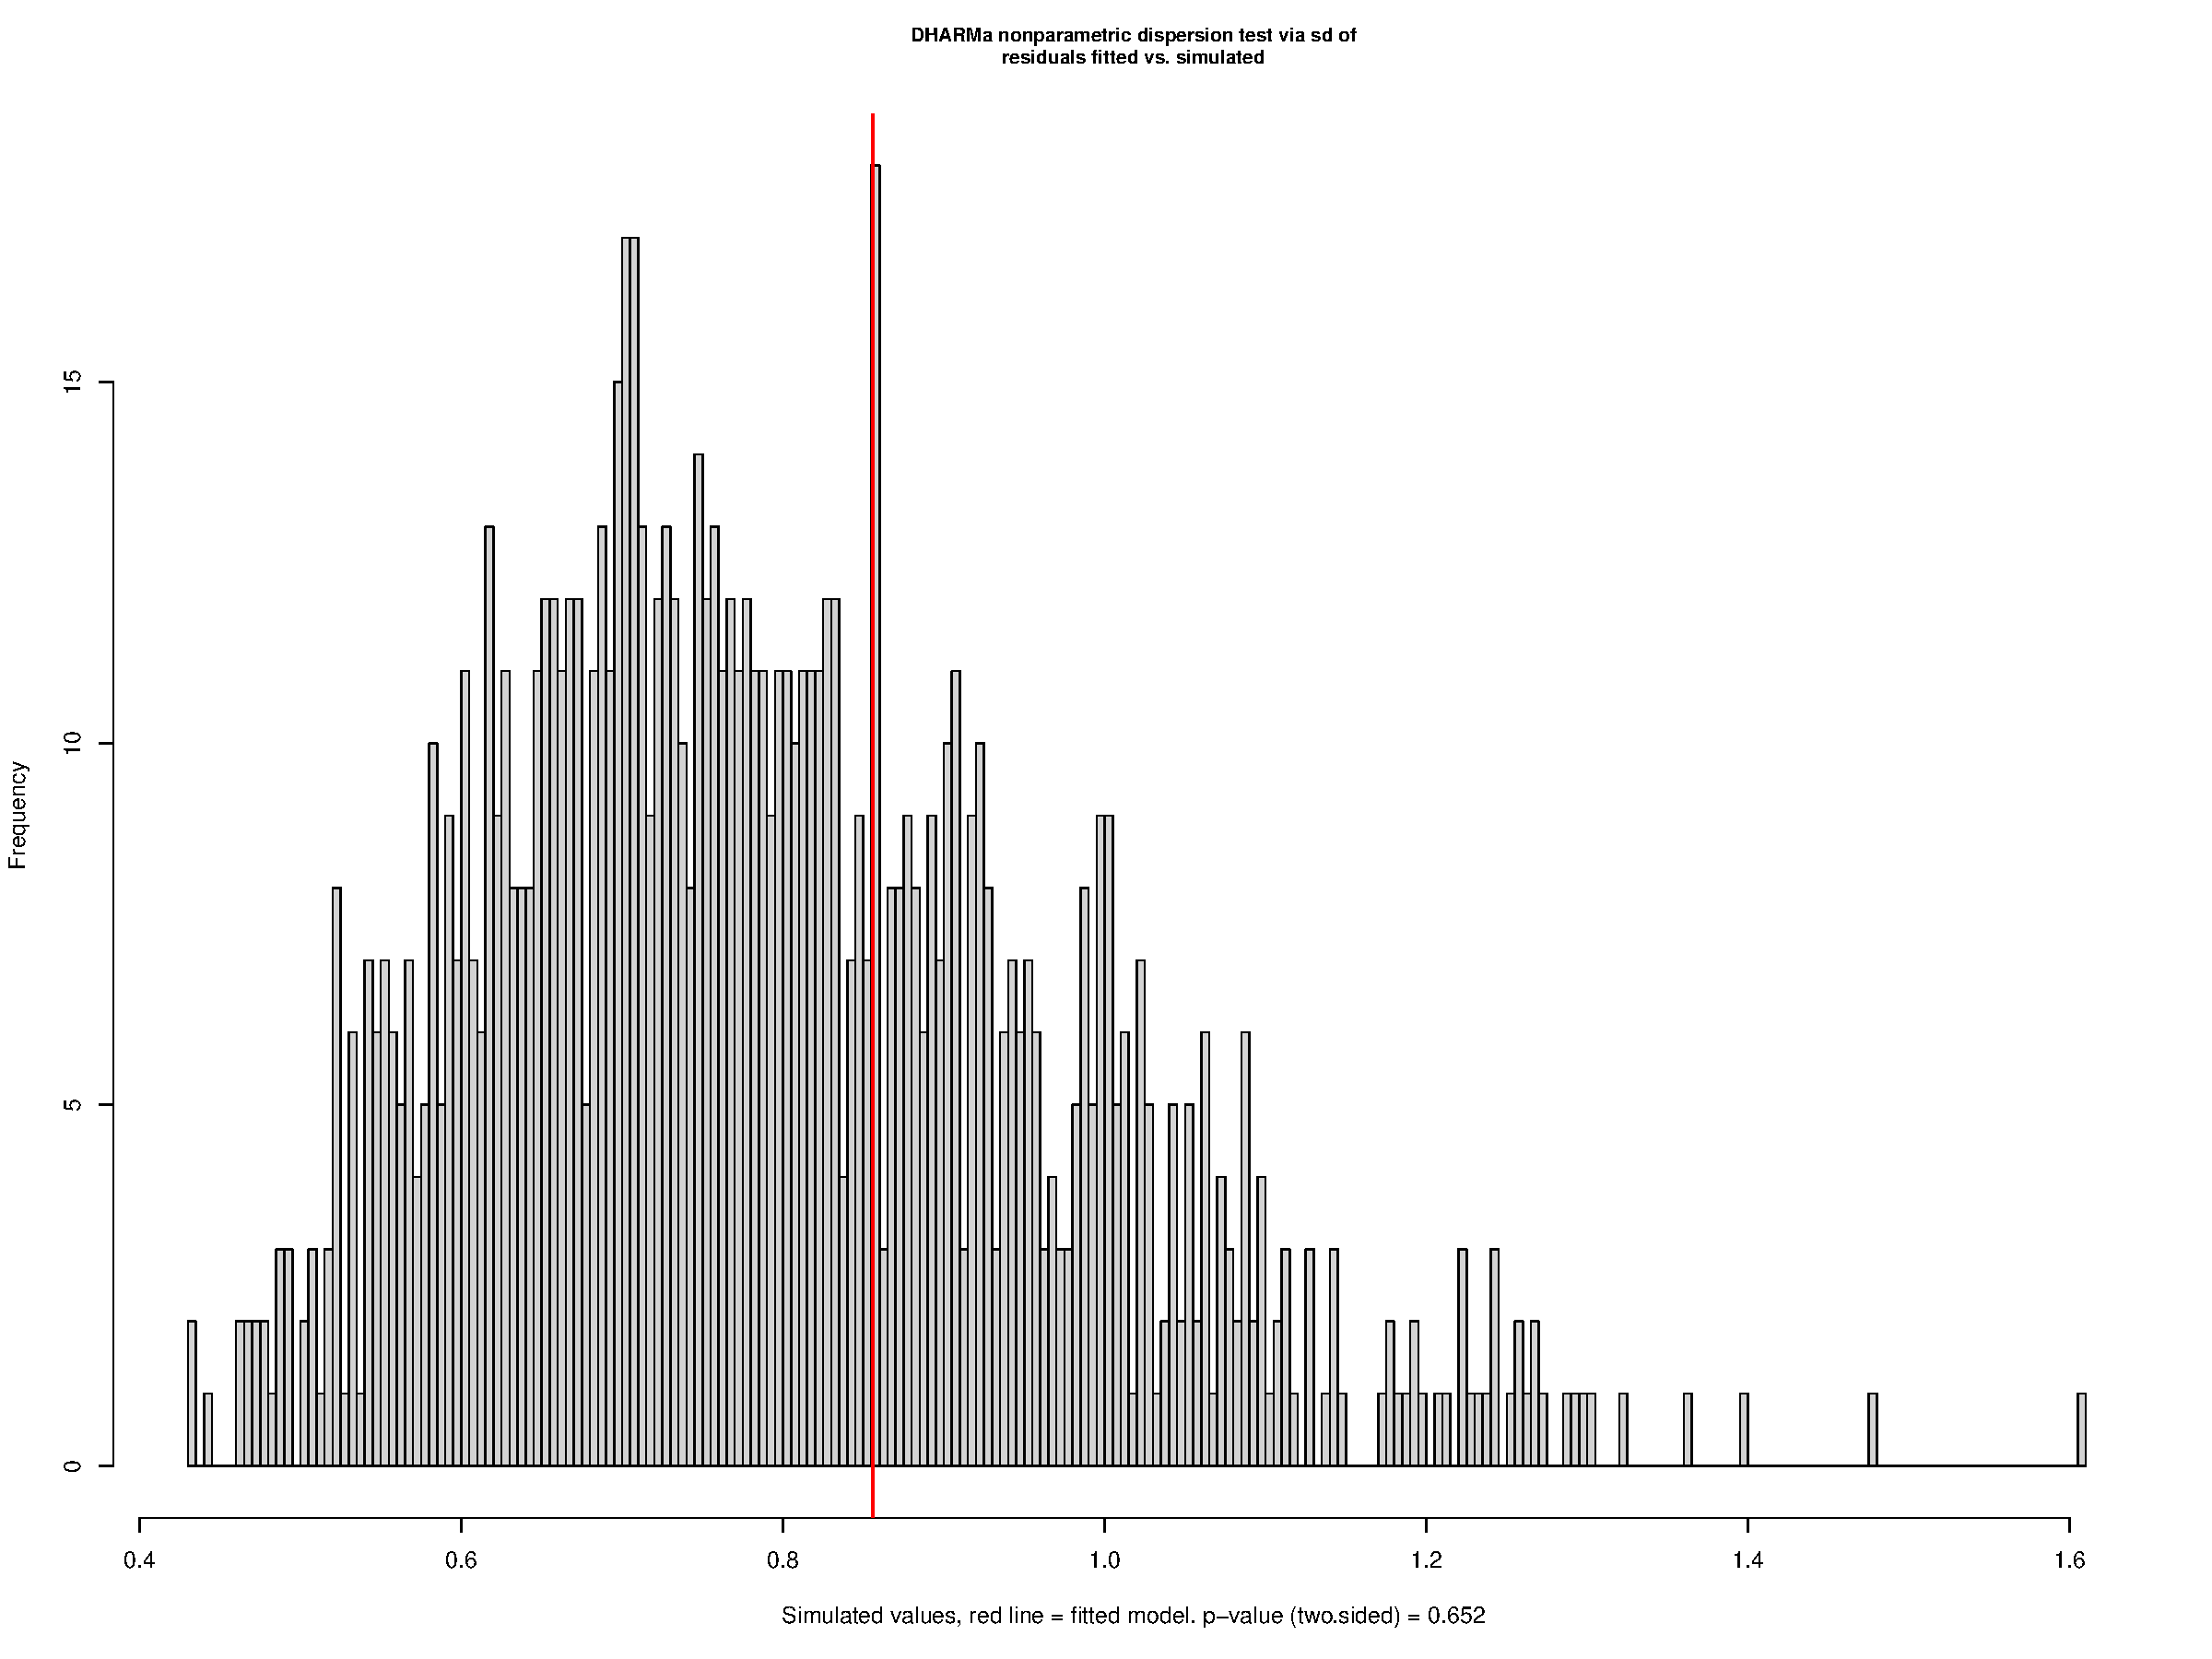
\includegraphics[keepaspectratio]{rsa_day1617_agar_files/figure-pdf/unnamed-chunk-3-6.pdf}}

\begin{verbatim}

    DHARMa nonparametric dispersion test via sd of residuals fitted vs.
    simulated

data:  simulationOutput
dispersion = 1.0792, p-value = 0.652
alternative hypothesis: two.sided
\end{verbatim}

\begin{Shaded}
\begin{Highlighting}[]
\FunctionTok{testZeroInflation}\NormalTok{(sim\_nb2)}
\end{Highlighting}
\end{Shaded}

\pandocbounded{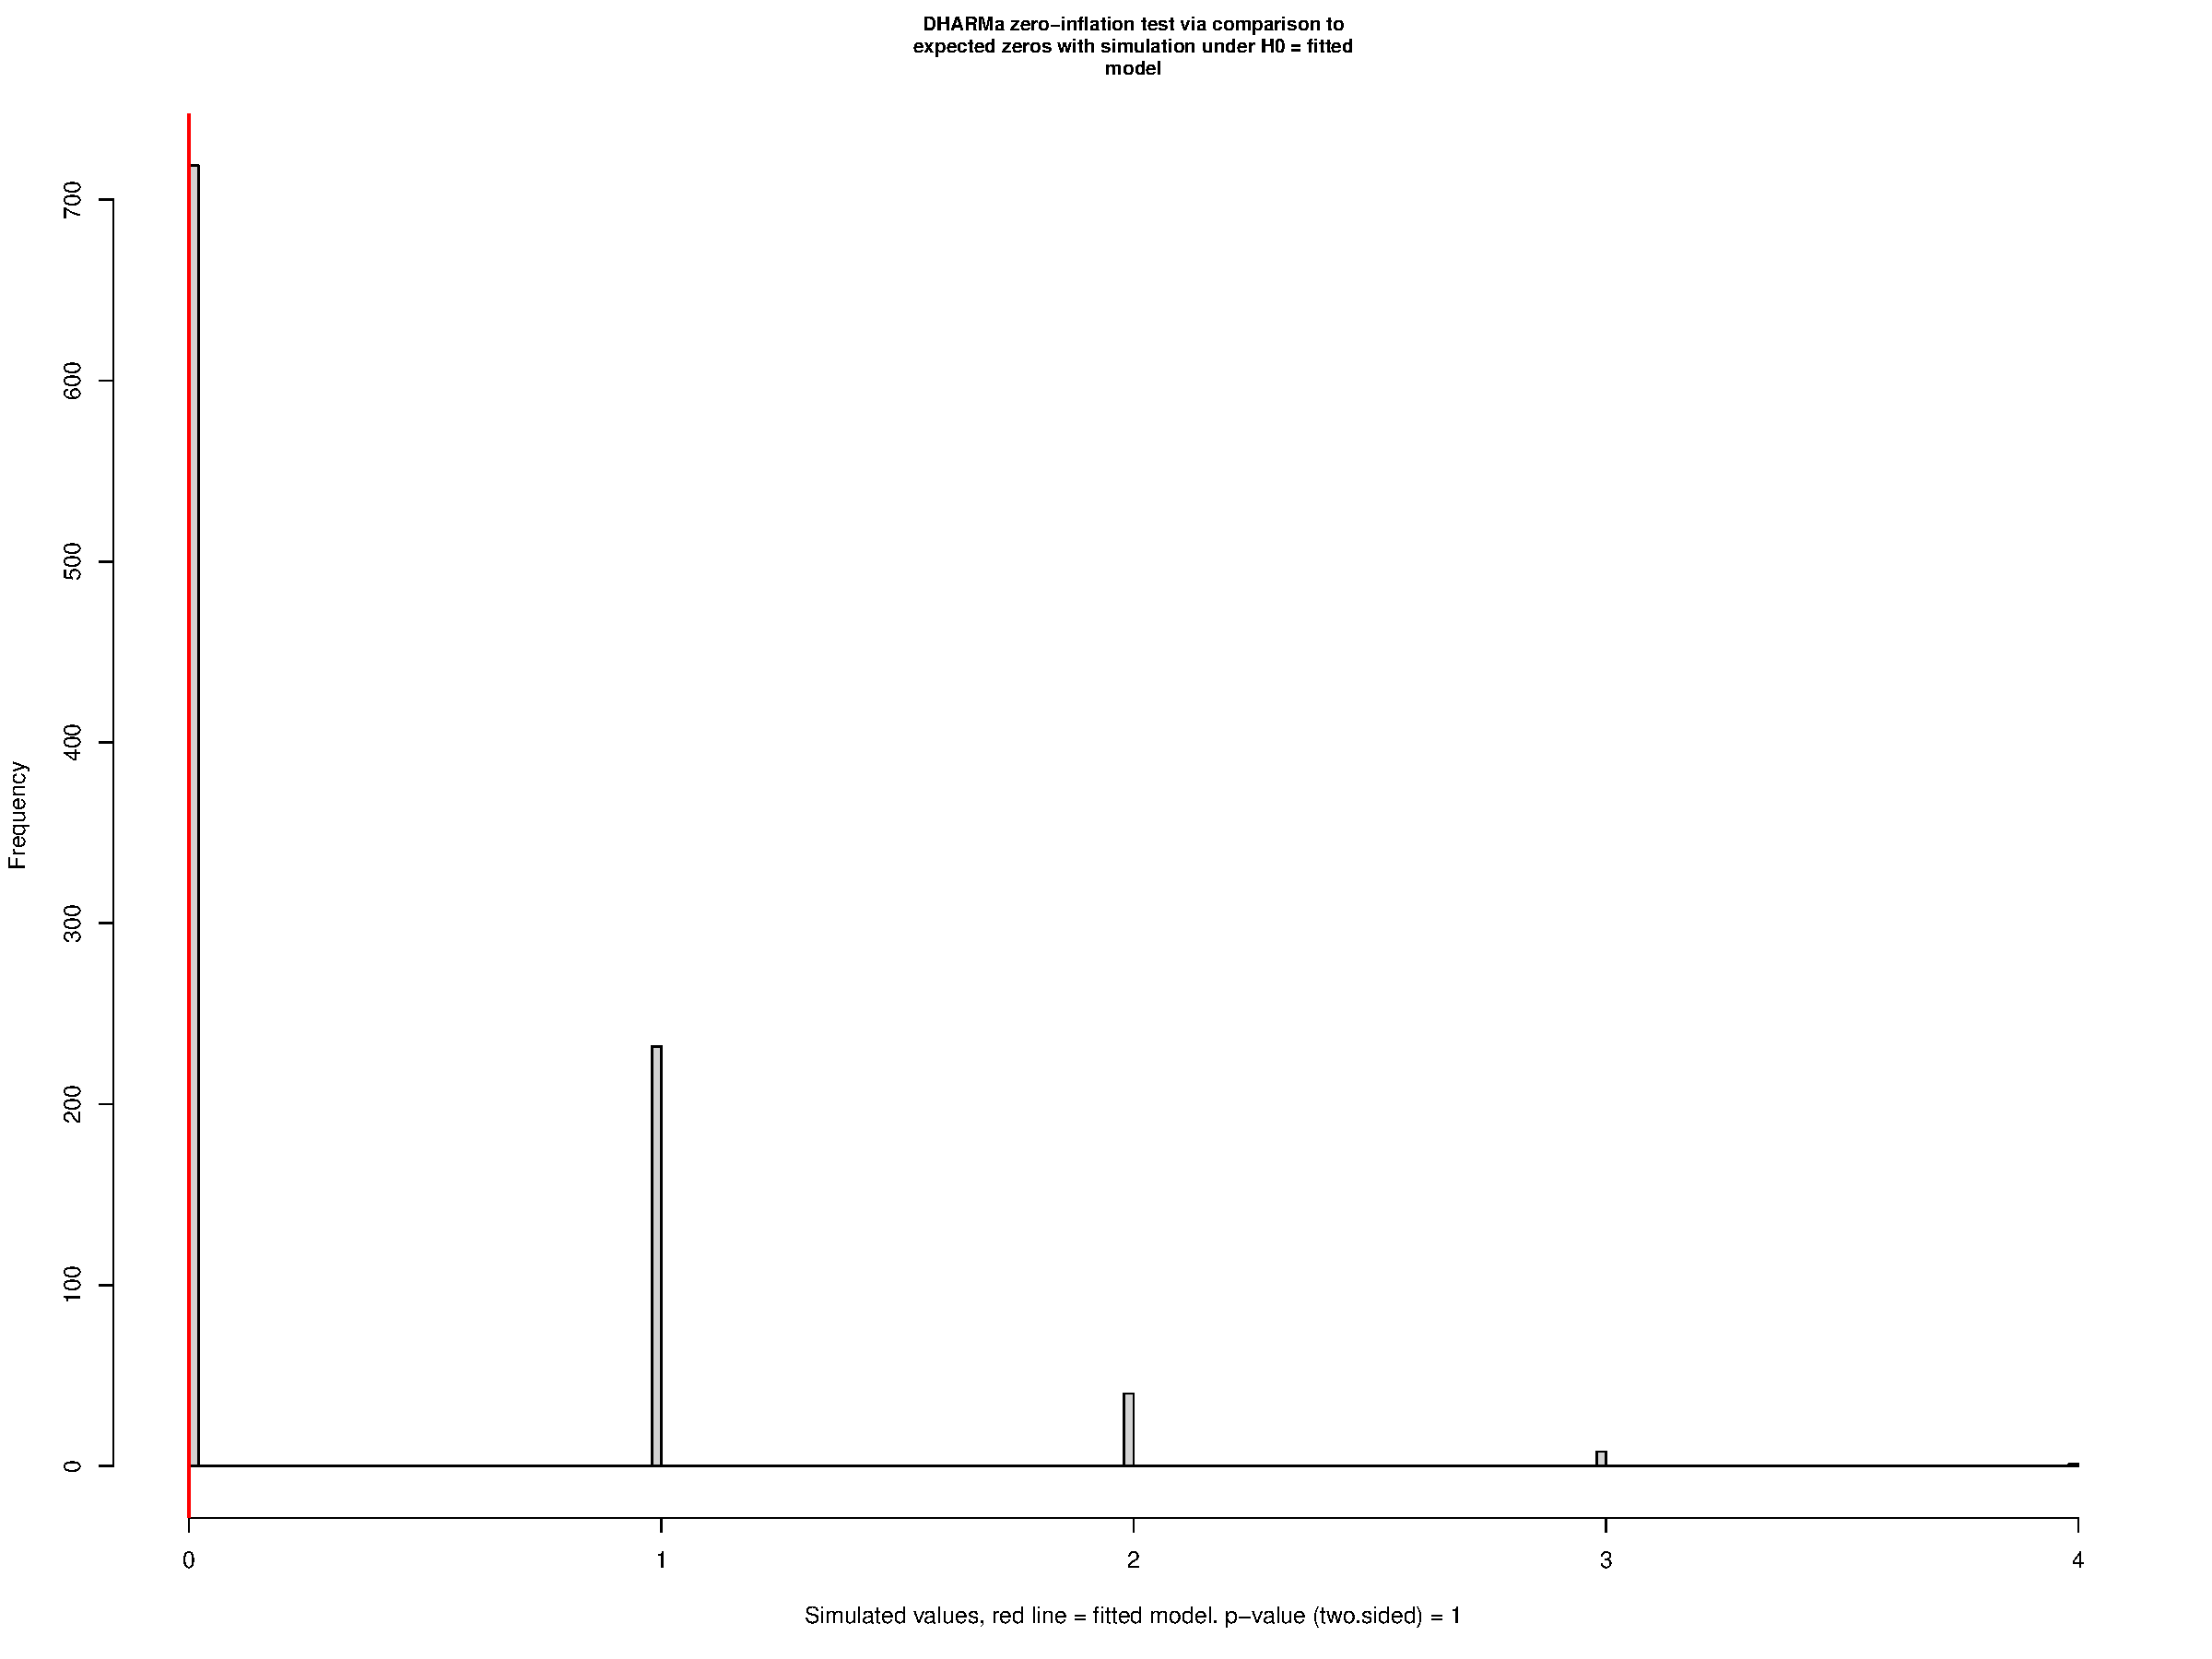
\includegraphics[keepaspectratio]{rsa_day1617_agar_files/figure-pdf/unnamed-chunk-3-7.pdf}}

\begin{verbatim}

    DHARMa zero-inflation test via comparison to expected zeros with
    simulation under H0 = fitted model

data:  simulationOutput
ratioObsSim = 0, p-value = 1
alternative hypothesis: two.sided
\end{verbatim}

\begin{Shaded}
\begin{Highlighting}[]
\FunctionTok{testOutliers}\NormalTok{(sim\_nb2)}
\end{Highlighting}
\end{Shaded}

\pandocbounded{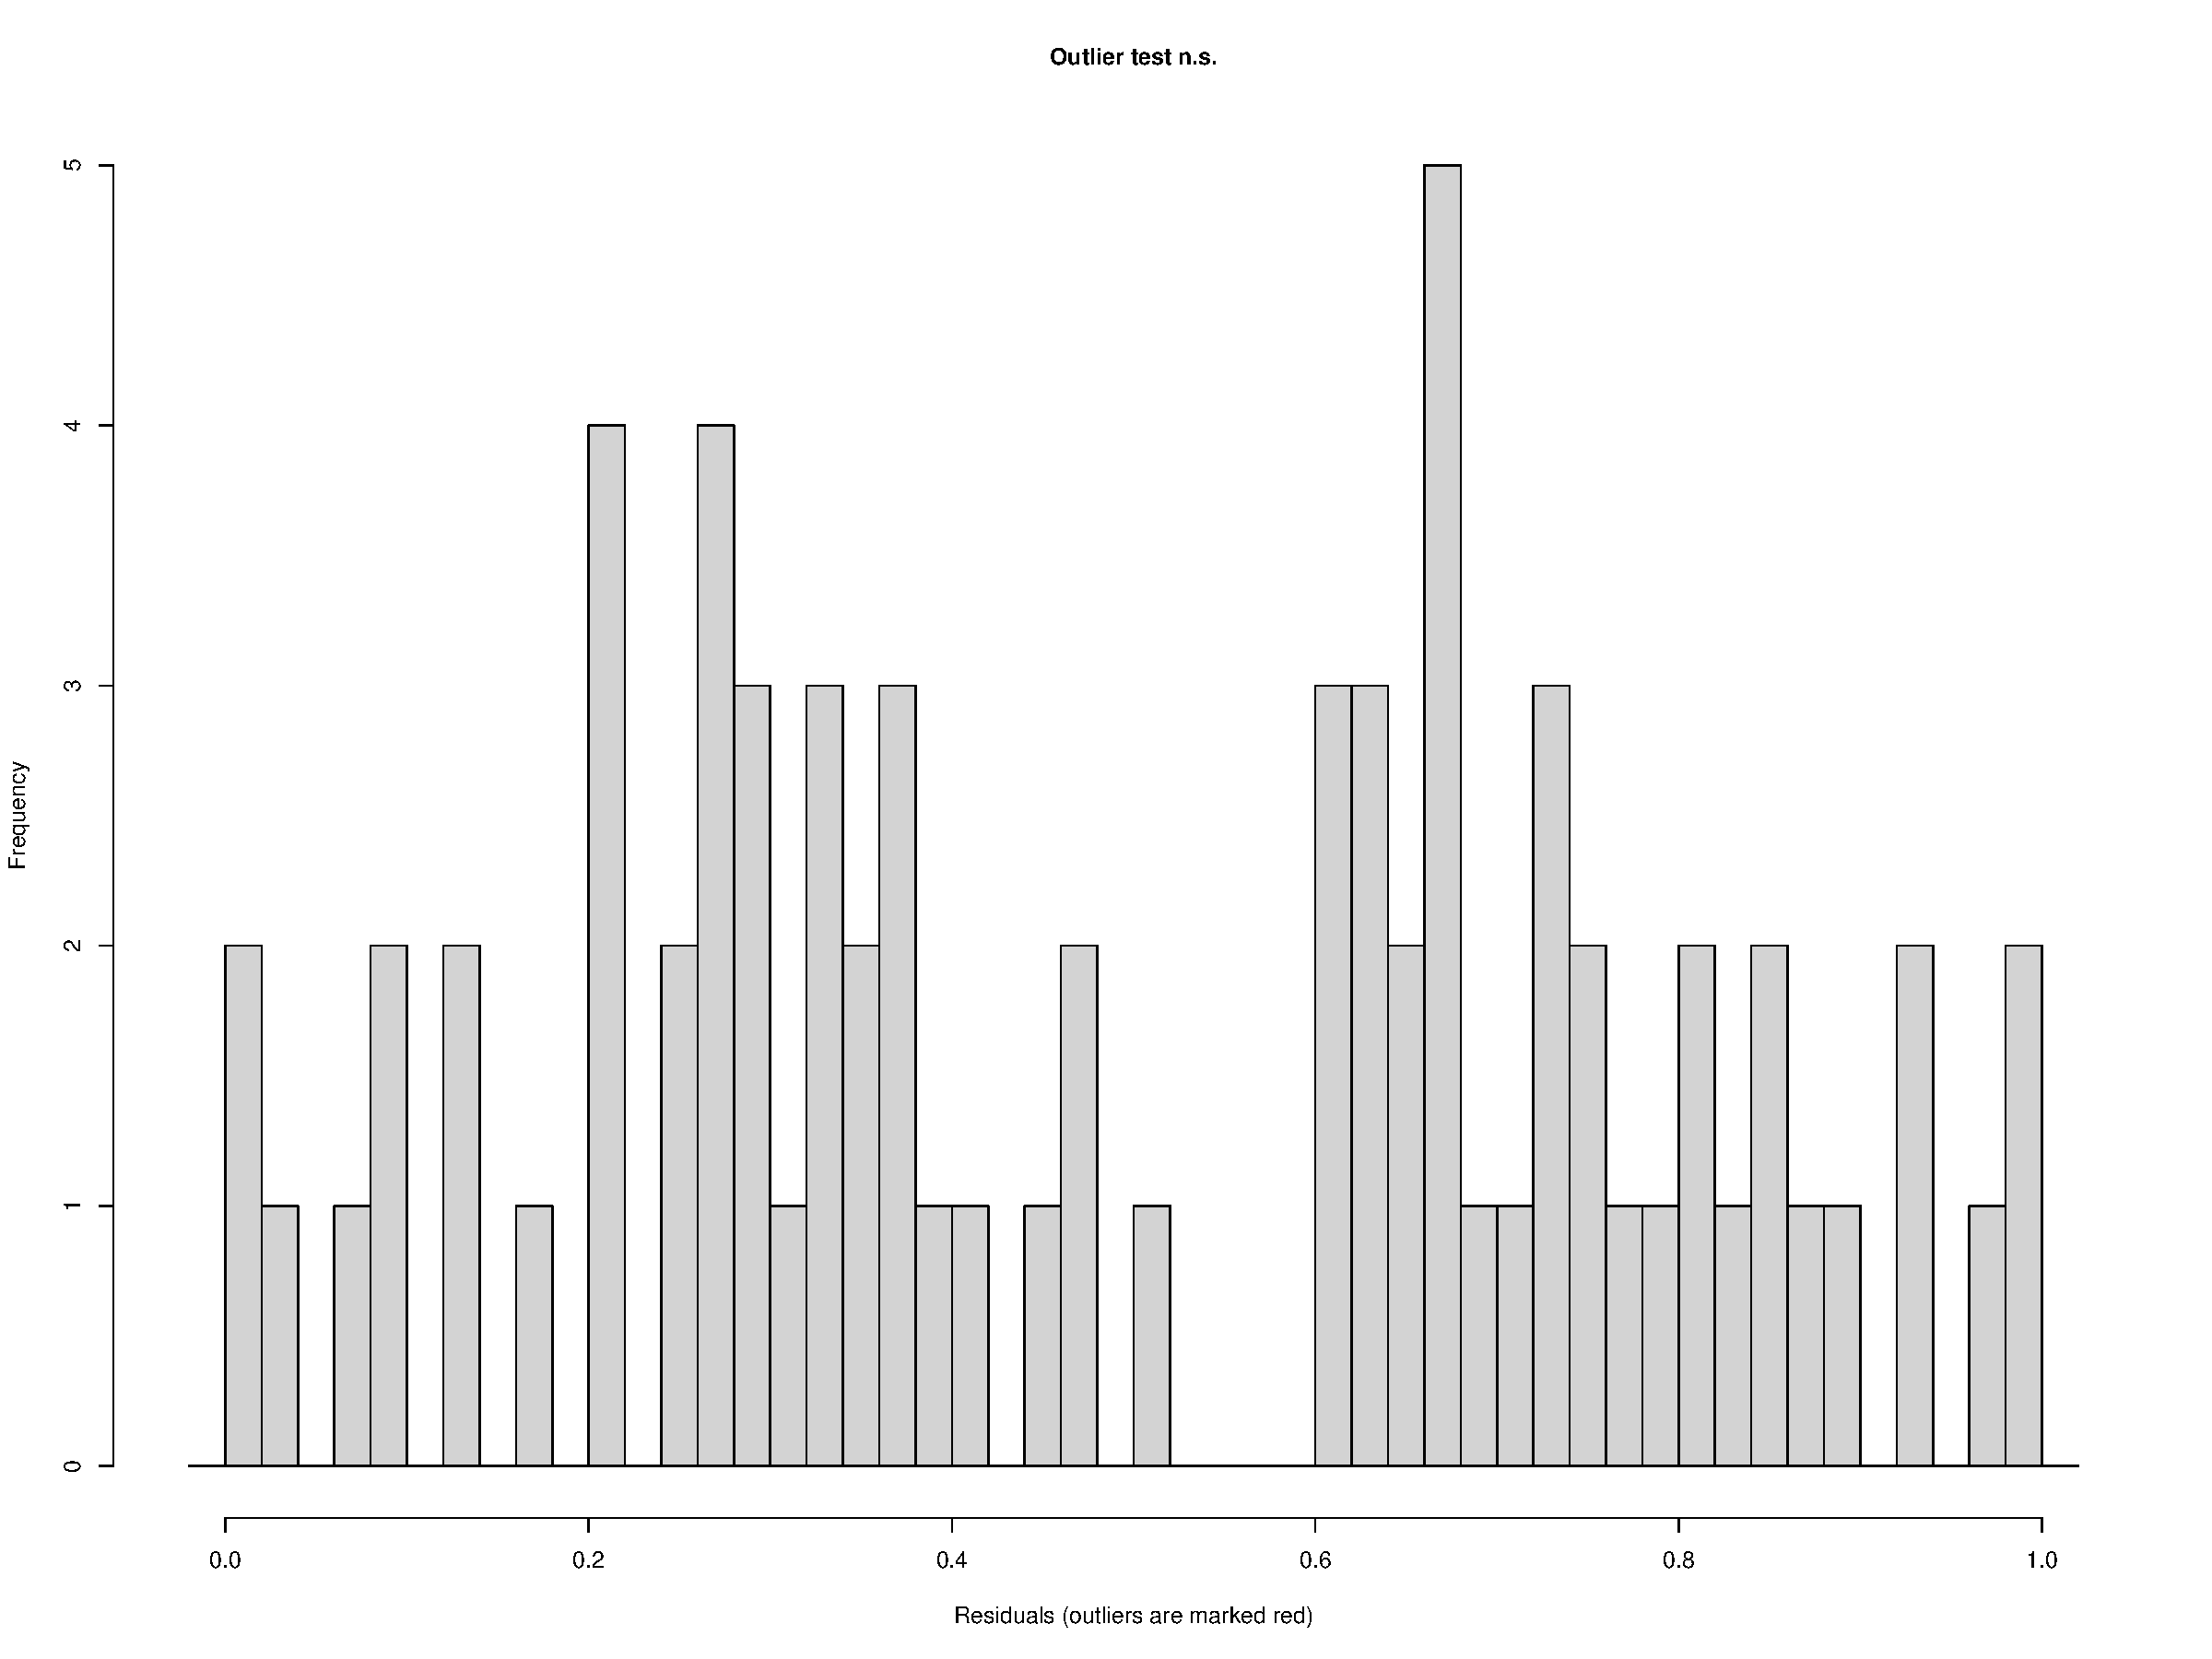
\includegraphics[keepaspectratio]{rsa_day1617_agar_files/figure-pdf/unnamed-chunk-3-8.pdf}}

\begin{verbatim}

    DHARMa bootstrapped outlier test

data:  sim_nb2
outliers at both margin(s) = 0, observations = 71, p-value = 1
alternative hypothesis: two.sided
 percent confidence interval:
 0.00000000 0.01408451
sample estimates:
outlier frequency (expected: 0.00126760563380282 ) 
                                                 0 
\end{verbatim}

\begin{Shaded}
\begin{Highlighting}[]
\CommentTok{\# residual plots show no significant deviation}

\CommentTok{\# ── 5. Random effects structure ───────────────────────────────}
\FunctionTok{VarCorr}\NormalTok{(tips\_tmb\_nb2)}
\end{Highlighting}
\end{Shaded}

\begin{verbatim}

Conditional model:
 Groups           Name        Std.Dev.  
 Seed:Plate:Batch (Intercept) 7.3231e-05
 Plate:Batch      (Intercept) 7.0113e-02
 Batch            (Intercept) 1.3790e-07
\end{verbatim}

\begin{Shaded}
\begin{Highlighting}[]
\FunctionTok{check\_singularity}\NormalTok{(tips\_tmb\_nb2) }
\end{Highlighting}
\end{Shaded}

\begin{verbatim}
[1] TRUE
\end{verbatim}

\begin{Shaded}
\begin{Highlighting}[]
\CommentTok{\# ── 7. Test Genotype effect + pairwise comparisons ────────────}
\CommentTok{\# emmeans gives estimated marginal means on the count scale}
\CommentTok{\# (type = "response" back{-}transforms from log link).}
\CommentTok{\# sidak HSD controls family{-}wise error rate across all pairs.}
\NormalTok{car}\SpecialCharTok{::}\FunctionTok{Anova}\NormalTok{(tips\_tmb\_nb2, }\AttributeTok{type =} \StringTok{"III"}\NormalTok{)}
\end{Highlighting}
\end{Shaded}

\begin{verbatim}
Analysis of Deviance Table (Type III Wald chisquare tests)

Response: Number.of.Root.Tips
              Chisq Df Pr(>Chisq)    
(Intercept) 276.856  1  < 2.2e-16 ***
Genotype     23.607  5  0.0002583 ***
---
Signif. codes:  0 '***' 0.001 '**' 0.01 '*' 0.05 '.' 0.1 ' ' 1
\end{verbatim}

\begin{Shaded}
\begin{Highlighting}[]
\NormalTok{emm }\OtherTok{\textless{}{-}} \FunctionTok{emmeans}\NormalTok{(tips\_tmb\_nb2, }\SpecialCharTok{\textasciitilde{}}\NormalTok{ Genotype, }\AttributeTok{type =} \StringTok{"response"}\NormalTok{)}
\FunctionTok{pairs}\NormalTok{(emm, }\AttributeTok{adjust =} \StringTok{"sidak"}\NormalTok{)}
\end{Highlighting}
\end{Shaded}

\begin{verbatim}
 contrast           ratio    SE  df null z.ratio p.value
 Addisie / Beten    1.127 0.222 Inf    1   0.608  1.0000
 Addisie / Dabbi    0.939 0.204 Inf    1  -0.289  1.0000
 Addisie / Karadebi 0.983 0.201 Inf    1  -0.085  1.0000
 Addisie / Manyi    1.105 0.268 Inf    1   0.413  1.0000
 Addisie / Tsedey   2.284 0.489 Inf    1   3.854  0.0017
 Beten / Dabbi      0.833 0.164 Inf    1  -0.926  0.9986
 Beten / Karadebi   0.872 0.167 Inf    1  -0.714  0.9999
 Beten / Manyi      0.981 0.224 Inf    1  -0.085  1.0000
 Beten / Tsedey     2.026 0.412 Inf    1   3.474  0.0077
 Dabbi / Karadebi   1.046 0.207 Inf    1   0.229  1.0000
 Dabbi / Manyi      1.177 0.271 Inf    1   0.707  0.9999
 Dabbi / Tsedey     2.432 0.522 Inf    1   4.141  0.0005
 Karadebi / Manyi   1.125 0.259 Inf    1   0.510  1.0000
 Karadebi / Tsedey  2.324 0.486 Inf    1   4.029  0.0008
 Manyi / Tsedey     2.066 0.502 Inf    1   2.987  0.0414

P value adjustment: sidak method for 15 tests 
Tests are performed on the log scale 
\end{verbatim}

\begin{Shaded}
\begin{Highlighting}[]
\NormalTok{cld\_df }\OtherTok{\textless{}{-}} \FunctionTok{as.data.frame}\NormalTok{(}\FunctionTok{cld}\NormalTok{(emm, }\AttributeTok{adjust =} \StringTok{"sidak"}\NormalTok{,}
                             \AttributeTok{Letters =}\NormalTok{ letters, }\AttributeTok{alpha =} \FloatTok{0.05}\NormalTok{)) }\SpecialCharTok{\%\textgreater{}\%}
  \FunctionTok{mutate}\NormalTok{(}\AttributeTok{.group =} \FunctionTok{trimws}\NormalTok{(.group))}

\FunctionTok{names}\NormalTok{(cld\_df)[}\FunctionTok{names}\NormalTok{(cld\_df) }\SpecialCharTok{\%in\%} \FunctionTok{c}\NormalTok{(}\StringTok{"asymp.LCL"}\NormalTok{, }\StringTok{"lower.CL"}\NormalTok{)] }\OtherTok{\textless{}{-}} \StringTok{"LCL"}
\FunctionTok{names}\NormalTok{(cld\_df)[}\FunctionTok{names}\NormalTok{(cld\_df) }\SpecialCharTok{\%in\%} \FunctionTok{c}\NormalTok{(}\StringTok{"asymp.UCL"}\NormalTok{, }\StringTok{"upper.CL"}\NormalTok{)] }\OtherTok{\textless{}{-}} \StringTok{"UCL"}

\NormalTok{n\_df }\OtherTok{\textless{}{-}}\NormalTok{ df }\SpecialCharTok{\%\textgreater{}\%}
  \FunctionTok{count}\NormalTok{(Genotype) }\SpecialCharTok{\%\textgreater{}\%}
  \FunctionTok{mutate}\NormalTok{(}\AttributeTok{label =} \FunctionTok{paste0}\NormalTok{(}\StringTok{"n="}\NormalTok{, n))}


\CommentTok{\# Effect size}

\CommentTok{\# Cohen\textquotesingle{}s d = difference in means / pooled SD}
\CommentTok{\# Interpretation: 0.2 = small, 0.5 = medium, 0.8 = large}

\NormalTok{emm\_tips }\OtherTok{\textless{}{-}} \FunctionTok{emmeans}\NormalTok{(tips\_tmb\_nb2, }\SpecialCharTok{\textasciitilde{}}\NormalTok{ Genotype)}

\NormalTok{eff\_tips }\OtherTok{\textless{}{-}} \FunctionTok{eff\_size}\NormalTok{(}
\NormalTok{  emm\_tips,}
  \AttributeTok{sigma =} \FunctionTok{sigma}\NormalTok{(tips\_tmb\_nb2),   }\CommentTok{\# residual SD from model}
  \AttributeTok{edf   =} \FunctionTok{df.residual}\NormalTok{(tips\_tmb\_nb2)}
\NormalTok{)}
\FunctionTok{print}\NormalTok{(eff\_tips)}
\end{Highlighting}
\end{Shaded}

\begin{verbatim}
 contrast           effect.size     SE  df asymp.LCL asymp.UCL
 Addisie - Beten        0.01695 0.0279 Inf   -0.0378    0.0717
 Addisie - Dabbi       -0.00891 0.0309 Inf   -0.0694    0.0516
 Addisie - Karadebi    -0.00248 0.0291 Inf   -0.0595    0.0545
 Addisie - Manyi        0.01418 0.0344 Inf   -0.0532    0.0816
 Addisie - Tsedey       0.11713 0.0322 Inf    0.0540    0.1802
 Beten - Dabbi         -0.02586 0.0280 Inf   -0.0808    0.0291
 Beten - Karadebi      -0.01944 0.0273 Inf   -0.0729    0.0341
 Beten - Manyi         -0.00277 0.0324 Inf   -0.0664    0.0608
 Beten - Tsedey         0.10017 0.0302 Inf    0.0409    0.1594
 Dabbi - Karadebi       0.00643 0.0280 Inf   -0.0485    0.0613
 Dabbi - Manyi          0.02309 0.0327 Inf   -0.0410    0.0872
 Dabbi - Tsedey         0.12603 0.0325 Inf    0.0623    0.1897
 Karadebi - Manyi       0.01666 0.0327 Inf   -0.0474    0.0808
 Karadebi - Tsedey      0.11961 0.0316 Inf    0.0577    0.1815
 Manyi - Tsedey         0.10295 0.0357 Inf    0.0330    0.1729

sigma used for effect sizes: 7.05 
Confidence level used: 0.95 
\end{verbatim}

\begin{Shaded}
\begin{Highlighting}[]
\CommentTok{\# all effect sizes are small }

\CommentTok{\# Summary stats needed for bar chart}
\NormalTok{bar\_df }\OtherTok{\textless{}{-}}\NormalTok{ df }\SpecialCharTok{\%\textgreater{}\%}
  \FunctionTok{group\_by}\NormalTok{(Genotype) }\SpecialCharTok{\%\textgreater{}\%}
  \FunctionTok{summarise}\NormalTok{(}\AttributeTok{mean\_tips =} \FunctionTok{mean}\NormalTok{(Number.of.Root.Tips),}
            \AttributeTok{se        =} \FunctionTok{sd}\NormalTok{(Number.of.Root.Tips) }\SpecialCharTok{/} \FunctionTok{sqrt}\NormalTok{(}\FunctionTok{n}\NormalTok{()),}
            \AttributeTok{.groups   =} \StringTok{"drop"}\NormalTok{)}


\CommentTok{\# ── 8. Plot 1 — Boxplot + jitter ─────────────────────────────}
\CommentTok{\# Boxplot shows full data distribution; jitter overlays raw points.}
\CommentTok{\# CLD letters indicate sidak groupings; shared letters = ns.}
\CommentTok{\# n labels below x{-}axis show sample sizes per genotype.}
\NormalTok{y\_ceil }\OtherTok{\textless{}{-}} \FunctionTok{max}\NormalTok{(df}\SpecialCharTok{$}\NormalTok{Number.of.Root.Tips) }\SpecialCharTok{*} \FloatTok{1.2}
\NormalTok{y\_label }\OtherTok{\textless{}{-}}\NormalTok{ y\_ceil }\SpecialCharTok{*} \FloatTok{0.86}

\NormalTok{p1 }\OtherTok{\textless{}{-}} \FunctionTok{ggplot}\NormalTok{(df, }\FunctionTok{aes}\NormalTok{(}\AttributeTok{x =}\NormalTok{ Genotype, }\AttributeTok{y =}\NormalTok{ Number.of.Root.Tips, }\AttributeTok{fill =}\NormalTok{ Genotype)) }\SpecialCharTok{+}

  \FunctionTok{geom\_boxplot}\NormalTok{(}
    \AttributeTok{alpha         =} \FloatTok{0.7}\NormalTok{,}
    \AttributeTok{outlier.shape =} \ConstantTok{NA}\NormalTok{,}
    \AttributeTok{width         =} \FloatTok{0.5}\NormalTok{,}
    \AttributeTok{colour        =} \StringTok{"black"}\NormalTok{,}
    \AttributeTok{linewidth     =} \FloatTok{0.5}
\NormalTok{  ) }\SpecialCharTok{+}

  \FunctionTok{geom\_jitter}\NormalTok{(}
    \AttributeTok{width  =} \FloatTok{0.15}\NormalTok{,}
    \AttributeTok{size   =} \FloatTok{1.8}\NormalTok{,}
    \AttributeTok{alpha  =} \FloatTok{0.55}\NormalTok{,}
    \AttributeTok{colour =} \StringTok{"black"}
\NormalTok{  ) }\SpecialCharTok{+}

  \FunctionTok{geom\_text}\NormalTok{(}
    \AttributeTok{data        =}\NormalTok{ cld\_df,}
    \FunctionTok{aes}\NormalTok{(}\AttributeTok{x =}\NormalTok{ Genotype, }\AttributeTok{label =}\NormalTok{ .group),}
    \AttributeTok{y           =}\NormalTok{ y\_label,}
    \AttributeTok{inherit.aes =} \ConstantTok{FALSE}\NormalTok{,}
    \AttributeTok{size        =} \DecValTok{9}\NormalTok{,}
    \AttributeTok{fontface    =} \StringTok{"bold"}\NormalTok{,}
    \AttributeTok{colour      =} \StringTok{"grey20"}
\NormalTok{  ) }\SpecialCharTok{+}

  \FunctionTok{geom\_text}\NormalTok{(}
    \AttributeTok{data        =}\NormalTok{ n\_df,}
    \FunctionTok{aes}\NormalTok{(}\AttributeTok{x =}\NormalTok{ Genotype, }\AttributeTok{label =}\NormalTok{ label),}
    \AttributeTok{y           =} \SpecialCharTok{{-}}\ConstantTok{Inf}\NormalTok{,}
    \AttributeTok{vjust       =} \FloatTok{4.2}\NormalTok{,}
    \AttributeTok{inherit.aes =} \ConstantTok{FALSE}\NormalTok{,}
    \AttributeTok{size        =} \DecValTok{6}\NormalTok{,}
    \AttributeTok{colour      =} \StringTok{"grey40"}
\NormalTok{  ) }\SpecialCharTok{+}

  \FunctionTok{scale\_fill\_brewer}\NormalTok{(}\AttributeTok{palette =} \StringTok{"Set2"}\NormalTok{) }\SpecialCharTok{+}

  \FunctionTok{labs}\NormalTok{(}
    \AttributeTok{x       =} \StringTok{"Genotype"}\NormalTok{,}
    \AttributeTok{y       =} \StringTok{"Number of root tips"}\NormalTok{,}
    \AttributeTok{caption =} \StringTok{"Shared letters indicate no significant difference (sidak HSD, p \textgreater{} 0.05; glmmTMB, nbinom2). Bars show raw means ± SE."}
\NormalTok{  ) }\SpecialCharTok{+}

  \FunctionTok{theme\_classic}\NormalTok{(}\AttributeTok{base\_size =} \DecValTok{14}\NormalTok{) }\SpecialCharTok{+}
  \FunctionTok{theme}\NormalTok{(}
    \AttributeTok{legend.position =} \StringTok{"none"}\NormalTok{,}
    \AttributeTok{panel.grid      =} \FunctionTok{element\_blank}\NormalTok{(),}
    \AttributeTok{axis.line       =} \FunctionTok{element\_line}\NormalTok{(}\AttributeTok{colour =} \StringTok{"black"}\NormalTok{, }\AttributeTok{linewidth =} \FloatTok{0.6}\NormalTok{),}
    \AttributeTok{axis.ticks      =} \FunctionTok{element\_line}\NormalTok{(}\AttributeTok{colour =} \StringTok{"black"}\NormalTok{, }\AttributeTok{linewidth =} \FloatTok{0.5}\NormalTok{),}
    \AttributeTok{axis.title      =} \FunctionTok{element\_text}\NormalTok{(}\AttributeTok{size =} \DecValTok{26}\NormalTok{, }\AttributeTok{face =} \StringTok{"bold"}\NormalTok{),}
    \AttributeTok{axis.title.x    =} \FunctionTok{element\_text}\NormalTok{(}\AttributeTok{size =} \DecValTok{26}\NormalTok{, }\AttributeTok{face =} \StringTok{"bold"}\NormalTok{, }\AttributeTok{margin =} \FunctionTok{margin}\NormalTok{(}\AttributeTok{t =} \DecValTok{24}\NormalTok{)),}
    \AttributeTok{axis.text       =} \FunctionTok{element\_text}\NormalTok{(}\AttributeTok{size =} \DecValTok{22}\NormalTok{, }\AttributeTok{colour =} \StringTok{"black"}\NormalTok{),}
    \AttributeTok{axis.text.x     =} \FunctionTok{element\_text}\NormalTok{(}\AttributeTok{face =} \StringTok{"italic"}\NormalTok{, }\AttributeTok{margin =} \FunctionTok{margin}\NormalTok{(}\AttributeTok{t =} \DecValTok{15}\NormalTok{)),}
    \AttributeTok{plot.caption    =} \FunctionTok{element\_text}\NormalTok{(}\AttributeTok{size =} \DecValTok{12}\NormalTok{, }\AttributeTok{colour =} \StringTok{"grey40"}\NormalTok{, }\AttributeTok{hjust =} \DecValTok{0}\NormalTok{, }\AttributeTok{margin =} \FunctionTok{margin}\NormalTok{(}\AttributeTok{t =} \DecValTok{10}\NormalTok{)),}
    \AttributeTok{plot.margin     =} \FunctionTok{margin}\NormalTok{(}\AttributeTok{t =} \DecValTok{25}\NormalTok{, }\AttributeTok{r =} \DecValTok{25}\NormalTok{, }\AttributeTok{b =} \DecValTok{25}\NormalTok{, }\AttributeTok{l =} \DecValTok{25}\NormalTok{)}
\NormalTok{  )}

\NormalTok{p1 }\SpecialCharTok{+} \FunctionTok{coord\_cartesian}\NormalTok{(}\AttributeTok{clip =} \StringTok{"off"}\NormalTok{)}
\end{Highlighting}
\end{Shaded}

\pandocbounded{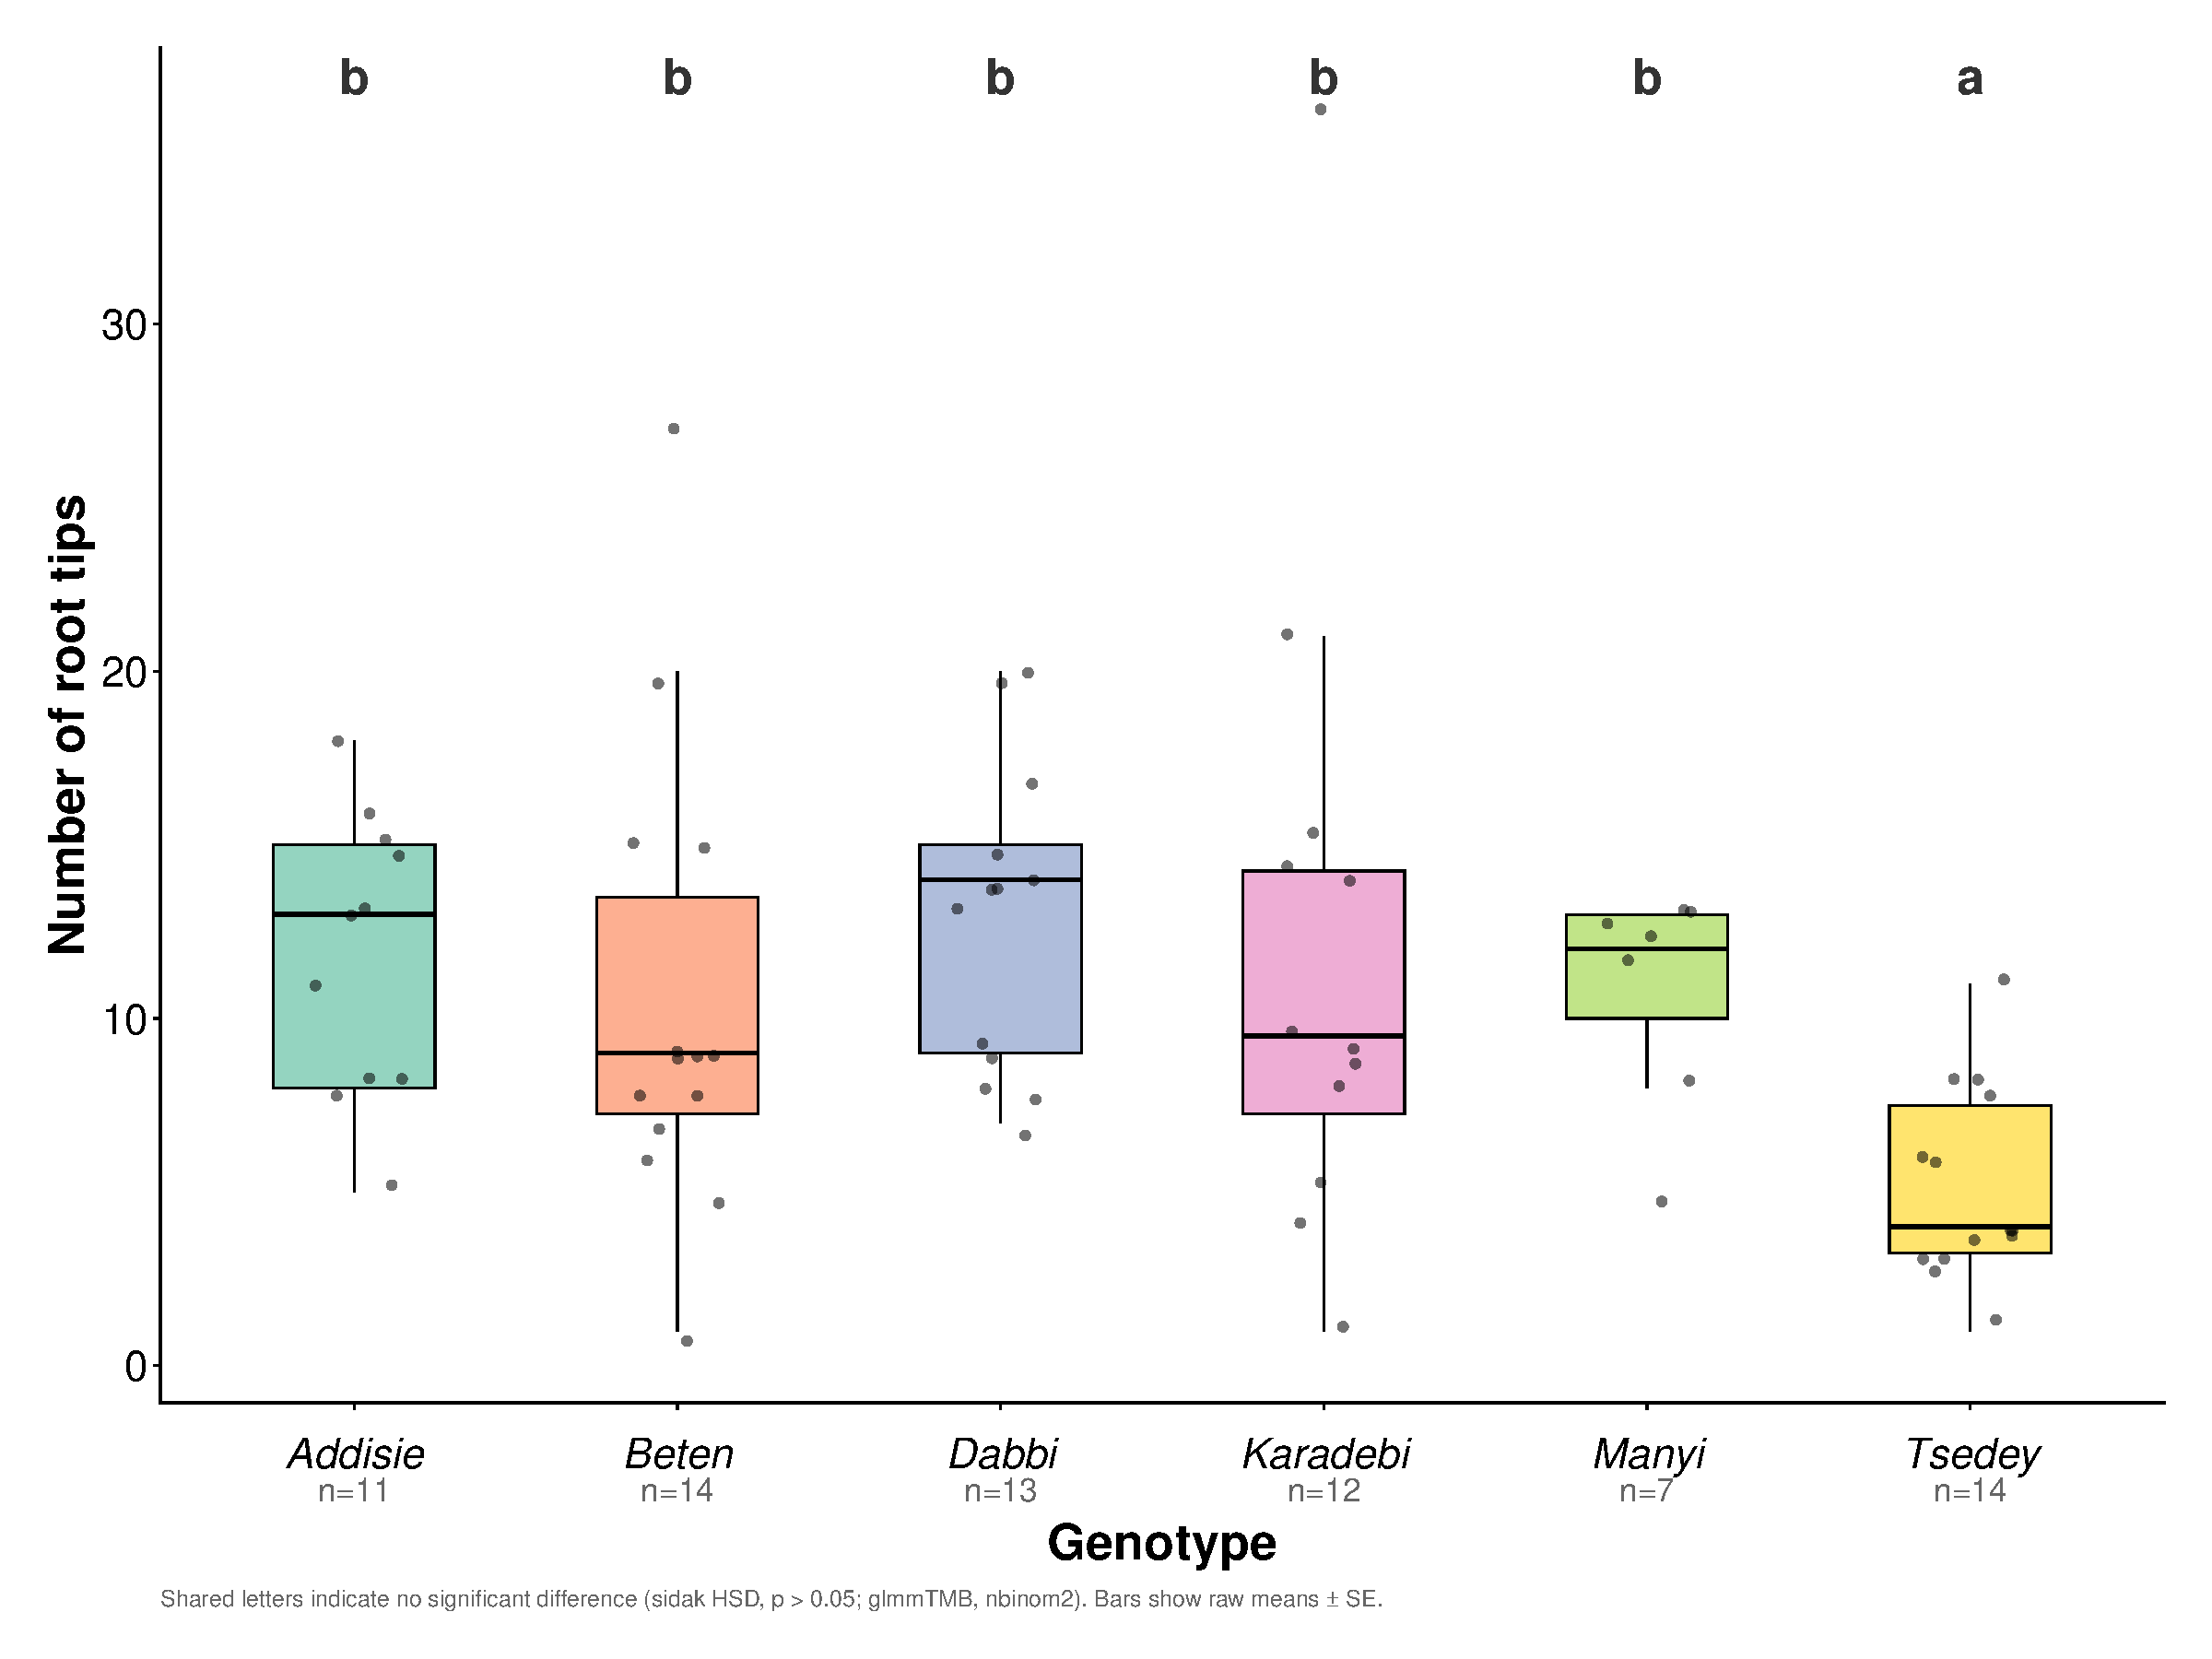
\includegraphics[keepaspectratio]{rsa_day1617_agar_files/figure-pdf/unnamed-chunk-3-9.pdf}}

\begin{Shaded}
\begin{Highlighting}[]
\CommentTok{\# ── 9. Plot 2 — Bar chart (mean ± SE) ────────────────────────}
\CommentTok{\# Bar chart shows mean ± 1 SE per genotype with raw data overlaid.}
\CommentTok{\# SE bars give a sense of within{-}genotype variability.}
\CommentTok{\# Raw points overlaid for transparency — avoids hiding the spread.}
\CommentTok{\# CLD letters from the mixed model placed above bars.}

\NormalTok{p2 }\OtherTok{\textless{}{-}} \FunctionTok{ggplot}\NormalTok{(bar\_df, }\FunctionTok{aes}\NormalTok{(}\AttributeTok{x =}\NormalTok{ Genotype, }\AttributeTok{y =}\NormalTok{ mean\_tips, }\AttributeTok{fill =}\NormalTok{ Genotype)) }\SpecialCharTok{+}

  \FunctionTok{geom\_col}\NormalTok{(}
    \AttributeTok{colour    =} \StringTok{"black"}\NormalTok{,}
    \AttributeTok{linewidth =} \FloatTok{0.3}\NormalTok{,}
    \AttributeTok{width     =} \FloatTok{0.5}\NormalTok{,}
    \AttributeTok{alpha     =} \FloatTok{0.8555}
\NormalTok{  ) }\SpecialCharTok{+}

  \FunctionTok{geom\_errorbar}\NormalTok{(}
    \FunctionTok{aes}\NormalTok{(}\AttributeTok{ymin =}\NormalTok{ mean\_tips }\SpecialCharTok{{-}}\NormalTok{ se, }\AttributeTok{ymax =}\NormalTok{ mean\_tips }\SpecialCharTok{+}\NormalTok{ se),}
    \AttributeTok{width     =} \FloatTok{0.2}\NormalTok{,}
    \AttributeTok{linewidth =} \FloatTok{0.3}\NormalTok{,}
    \AttributeTok{colour    =} \StringTok{"black"}
\NormalTok{  ) }\SpecialCharTok{+}

  \CommentTok{\# Raw data overlaid for transparency}
  \FunctionTok{geom\_jitter}\NormalTok{(}
    \AttributeTok{data   =}\NormalTok{ df,}
    \FunctionTok{aes}\NormalTok{(}\AttributeTok{x =}\NormalTok{ Genotype, }\AttributeTok{y =}\NormalTok{ Number.of.Root.Tips),}
    \AttributeTok{width  =} \FloatTok{0.15}\NormalTok{,}
    \AttributeTok{size   =} \FloatTok{1.3}\NormalTok{,}
    \AttributeTok{alpha  =} \FloatTok{0.55}\NormalTok{,}
    \AttributeTok{colour =} \StringTok{"black"}\NormalTok{,}
    \AttributeTok{inherit.aes =} \ConstantTok{FALSE}
\NormalTok{  ) }\SpecialCharTok{+}

  \FunctionTok{geom\_text}\NormalTok{(}
    \AttributeTok{data        =}\NormalTok{ cld\_df,}
    \FunctionTok{aes}\NormalTok{(}\AttributeTok{x =}\NormalTok{ Genotype, }\AttributeTok{label =}\NormalTok{ .group),}
    \AttributeTok{y           =} \FunctionTok{max}\NormalTok{(df}\SpecialCharTok{$}\NormalTok{Number.of.Root.Tips, }\AttributeTok{na.rm =} \ConstantTok{TRUE}\NormalTok{) }\SpecialCharTok{*} \FloatTok{1.02}\NormalTok{,}
    \AttributeTok{inherit.aes =} \ConstantTok{FALSE}\NormalTok{,}
    \AttributeTok{size        =} \DecValTok{5}\NormalTok{,}
    \AttributeTok{fontface    =} \StringTok{"bold"}\NormalTok{,}
    \AttributeTok{colour      =} \StringTok{"grey20"}
\NormalTok{  ) }\SpecialCharTok{+}

  \FunctionTok{geom\_text}\NormalTok{(}
    \AttributeTok{data        =}\NormalTok{ n\_df,}
    \FunctionTok{aes}\NormalTok{(}\AttributeTok{x =}\NormalTok{ Genotype, }\AttributeTok{label =}\NormalTok{ label),}
    \AttributeTok{y           =} \SpecialCharTok{{-}}\ConstantTok{Inf}\NormalTok{,}
    \AttributeTok{vjust       =} \FloatTok{4.2}\NormalTok{,}
    \AttributeTok{inherit.aes =} \ConstantTok{FALSE}\NormalTok{,}
    \AttributeTok{size        =} \FloatTok{3.5}\NormalTok{,}
    \AttributeTok{colour      =} \StringTok{"grey40"}
\NormalTok{  ) }\SpecialCharTok{+}

  \FunctionTok{scale\_fill\_brewer}\NormalTok{(}\AttributeTok{palette =} \StringTok{"Set2"}\NormalTok{) }\SpecialCharTok{+}

  \FunctionTok{labs}\NormalTok{(}
    \AttributeTok{x       =} \StringTok{"Genotype"}\NormalTok{,}
    \AttributeTok{y       =} \StringTok{"Number of root tips"}\NormalTok{,}
    \AttributeTok{caption =} \StringTok{"Bars = mean ± 1 SE; points = raw data}\SpecialCharTok{\textbackslash{}n}\StringTok{Shared letters indicate no significant difference (sidak HSD, p \textgreater{} 0.05; glmmTMB, nbinom2)"}
\NormalTok{  ) }\SpecialCharTok{+}

  \FunctionTok{theme\_classic}\NormalTok{(}\AttributeTok{base\_size =} \DecValTok{18}\NormalTok{) }\SpecialCharTok{+}
  \FunctionTok{theme}\NormalTok{(}
    \AttributeTok{legend.position =} \StringTok{"none"}\NormalTok{,}
    \AttributeTok{panel.grid      =} \FunctionTok{element\_blank}\NormalTok{(),}
    \AttributeTok{axis.line       =} \FunctionTok{element\_line}\NormalTok{(}\AttributeTok{colour =} \StringTok{"black"}\NormalTok{, }\AttributeTok{linewidth =} \FloatTok{0.6}\NormalTok{),}
    \AttributeTok{axis.ticks      =} \FunctionTok{element\_line}\NormalTok{(}\AttributeTok{colour =} \StringTok{"black"}\NormalTok{, }\AttributeTok{linewidth =} \FloatTok{0.5}\NormalTok{),}
    \AttributeTok{axis.title      =} \FunctionTok{element\_text}\NormalTok{(}\AttributeTok{size =} \DecValTok{16}\NormalTok{, }\AttributeTok{face =} \StringTok{"bold"}\NormalTok{),}
    \AttributeTok{axis.text       =} \FunctionTok{element\_text}\NormalTok{(}\AttributeTok{size =} \DecValTok{16}\NormalTok{, }\AttributeTok{colour =} \StringTok{"black"}\NormalTok{),}
    \AttributeTok{axis.text.x     =} \FunctionTok{element\_text}\NormalTok{(}\AttributeTok{face =} \StringTok{"italic"}\NormalTok{, }\AttributeTok{margin =} \FunctionTok{margin}\NormalTok{(}\AttributeTok{t =} \DecValTok{3}\NormalTok{)),}
    \AttributeTok{plot.caption    =} \FunctionTok{element\_text}\NormalTok{(}\AttributeTok{size =} \DecValTok{12}\NormalTok{, }\AttributeTok{colour =} \StringTok{"grey40"}\NormalTok{, }\AttributeTok{hjust =} \DecValTok{0}\NormalTok{),}
    \AttributeTok{plot.margin     =} \FunctionTok{margin}\NormalTok{(}\AttributeTok{t =} \DecValTok{10}\NormalTok{, }\AttributeTok{r =} \DecValTok{15}\NormalTok{, }\AttributeTok{b =} \DecValTok{30}\NormalTok{, }\AttributeTok{l =} \DecValTok{10}\NormalTok{)}
\NormalTok{  )}

\NormalTok{p2 }\SpecialCharTok{+} \FunctionTok{coord\_cartesian}\NormalTok{(}\AttributeTok{clip =} \StringTok{"off"}\NormalTok{)}
\end{Highlighting}
\end{Shaded}

\pandocbounded{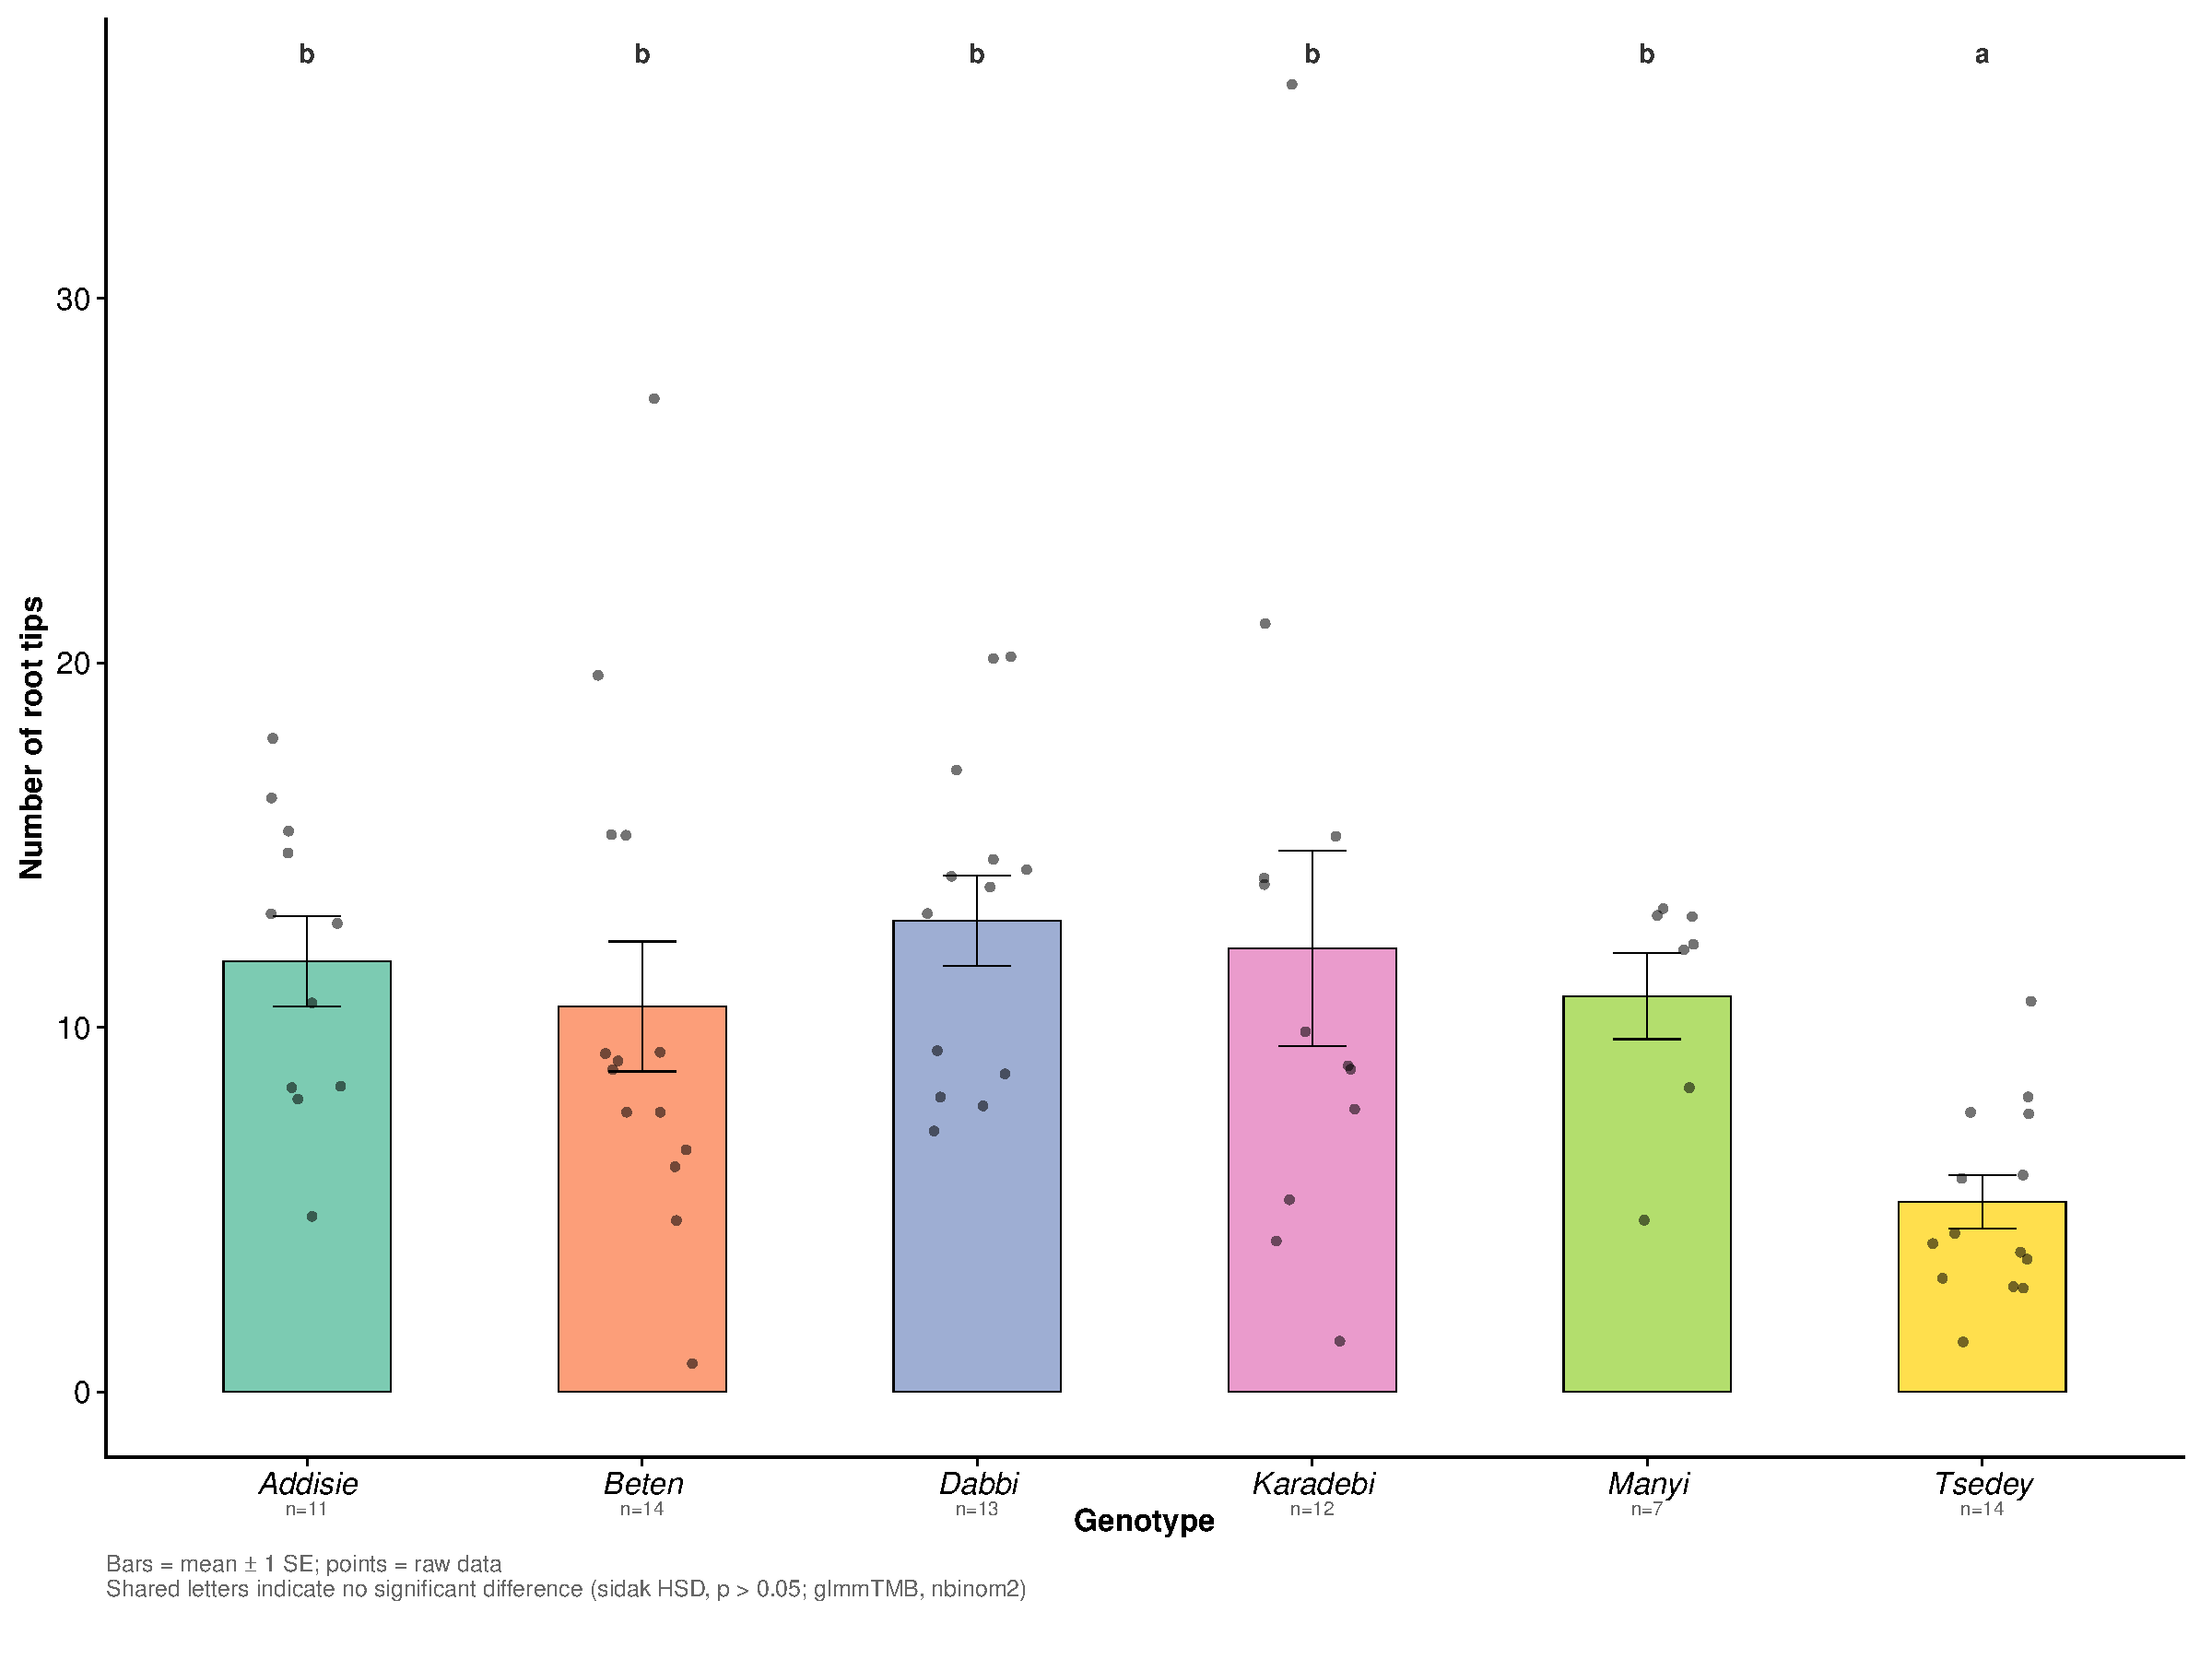
\includegraphics[keepaspectratio]{rsa_day1617_agar_files/figure-pdf/unnamed-chunk-3-10.pdf}}

\subsubsection{Average Root Diameter}\label{average-root-diameter}

\begin{Shaded}
\begin{Highlighting}[]
\NormalTok{df }\SpecialCharTok{\%\textgreater{}\%}
  \FunctionTok{group\_by}\NormalTok{(Genotype) }\SpecialCharTok{\%\textgreater{}\%}
  \FunctionTok{summarise}\NormalTok{(}\AttributeTok{Mean     =} \FunctionTok{round}\NormalTok{(}\FunctionTok{mean}\NormalTok{(Average.Diameter.mm), }\DecValTok{2}\NormalTok{),}
            \AttributeTok{Variance =} \FunctionTok{round}\NormalTok{(}\FunctionTok{var}\NormalTok{(Average.Diameter.mm),  }\DecValTok{2}\NormalTok{),}
            \AttributeTok{Var\_Mean =} \FunctionTok{round}\NormalTok{(}\FunctionTok{var}\NormalTok{(Average.Diameter.mm) }\SpecialCharTok{/}
                               \FunctionTok{mean}\NormalTok{(Average.Diameter.mm), }\DecValTok{2}\NormalTok{))}
\end{Highlighting}
\end{Shaded}

\begin{verbatim}
# A tibble: 6 x 4
  Genotype  Mean Variance Var_Mean
  <fct>    <dbl>    <dbl>    <dbl>
1 Addisie   0.22        0     0.01
2 Beten     0.23        0     0.01
3 Dabbi     0.2         0     0.01
4 Karadebi  0.21        0     0   
5 Manyi     0.27        0     0.01
6 Tsedey    0.23        0     0.01
\end{verbatim}

\begin{Shaded}
\begin{Highlighting}[]
\CommentTok{\# Histogram}
\FunctionTok{ggplot}\NormalTok{(df, }\FunctionTok{aes}\NormalTok{(}\AttributeTok{x =}\NormalTok{ Average.Diameter.mm)) }\SpecialCharTok{+}
  \FunctionTok{geom\_histogram}\NormalTok{(}\AttributeTok{bins =} \DecValTok{15}\NormalTok{, }\AttributeTok{fill =} \StringTok{"\#66C2A5"}\NormalTok{, }\AttributeTok{colour =} \StringTok{"white"}\NormalTok{) }\SpecialCharTok{+}
  \FunctionTok{labs}\NormalTok{(}\AttributeTok{title =} \StringTok{"Distribution of Average Root Diameter"}\NormalTok{,}
       \AttributeTok{x =} \StringTok{"Average Diameter (mm)"}\NormalTok{, }\AttributeTok{y =} \StringTok{"Count"}\NormalTok{) }\SpecialCharTok{+}
  \FunctionTok{theme\_bw}\NormalTok{()}
\end{Highlighting}
\end{Shaded}

\pandocbounded{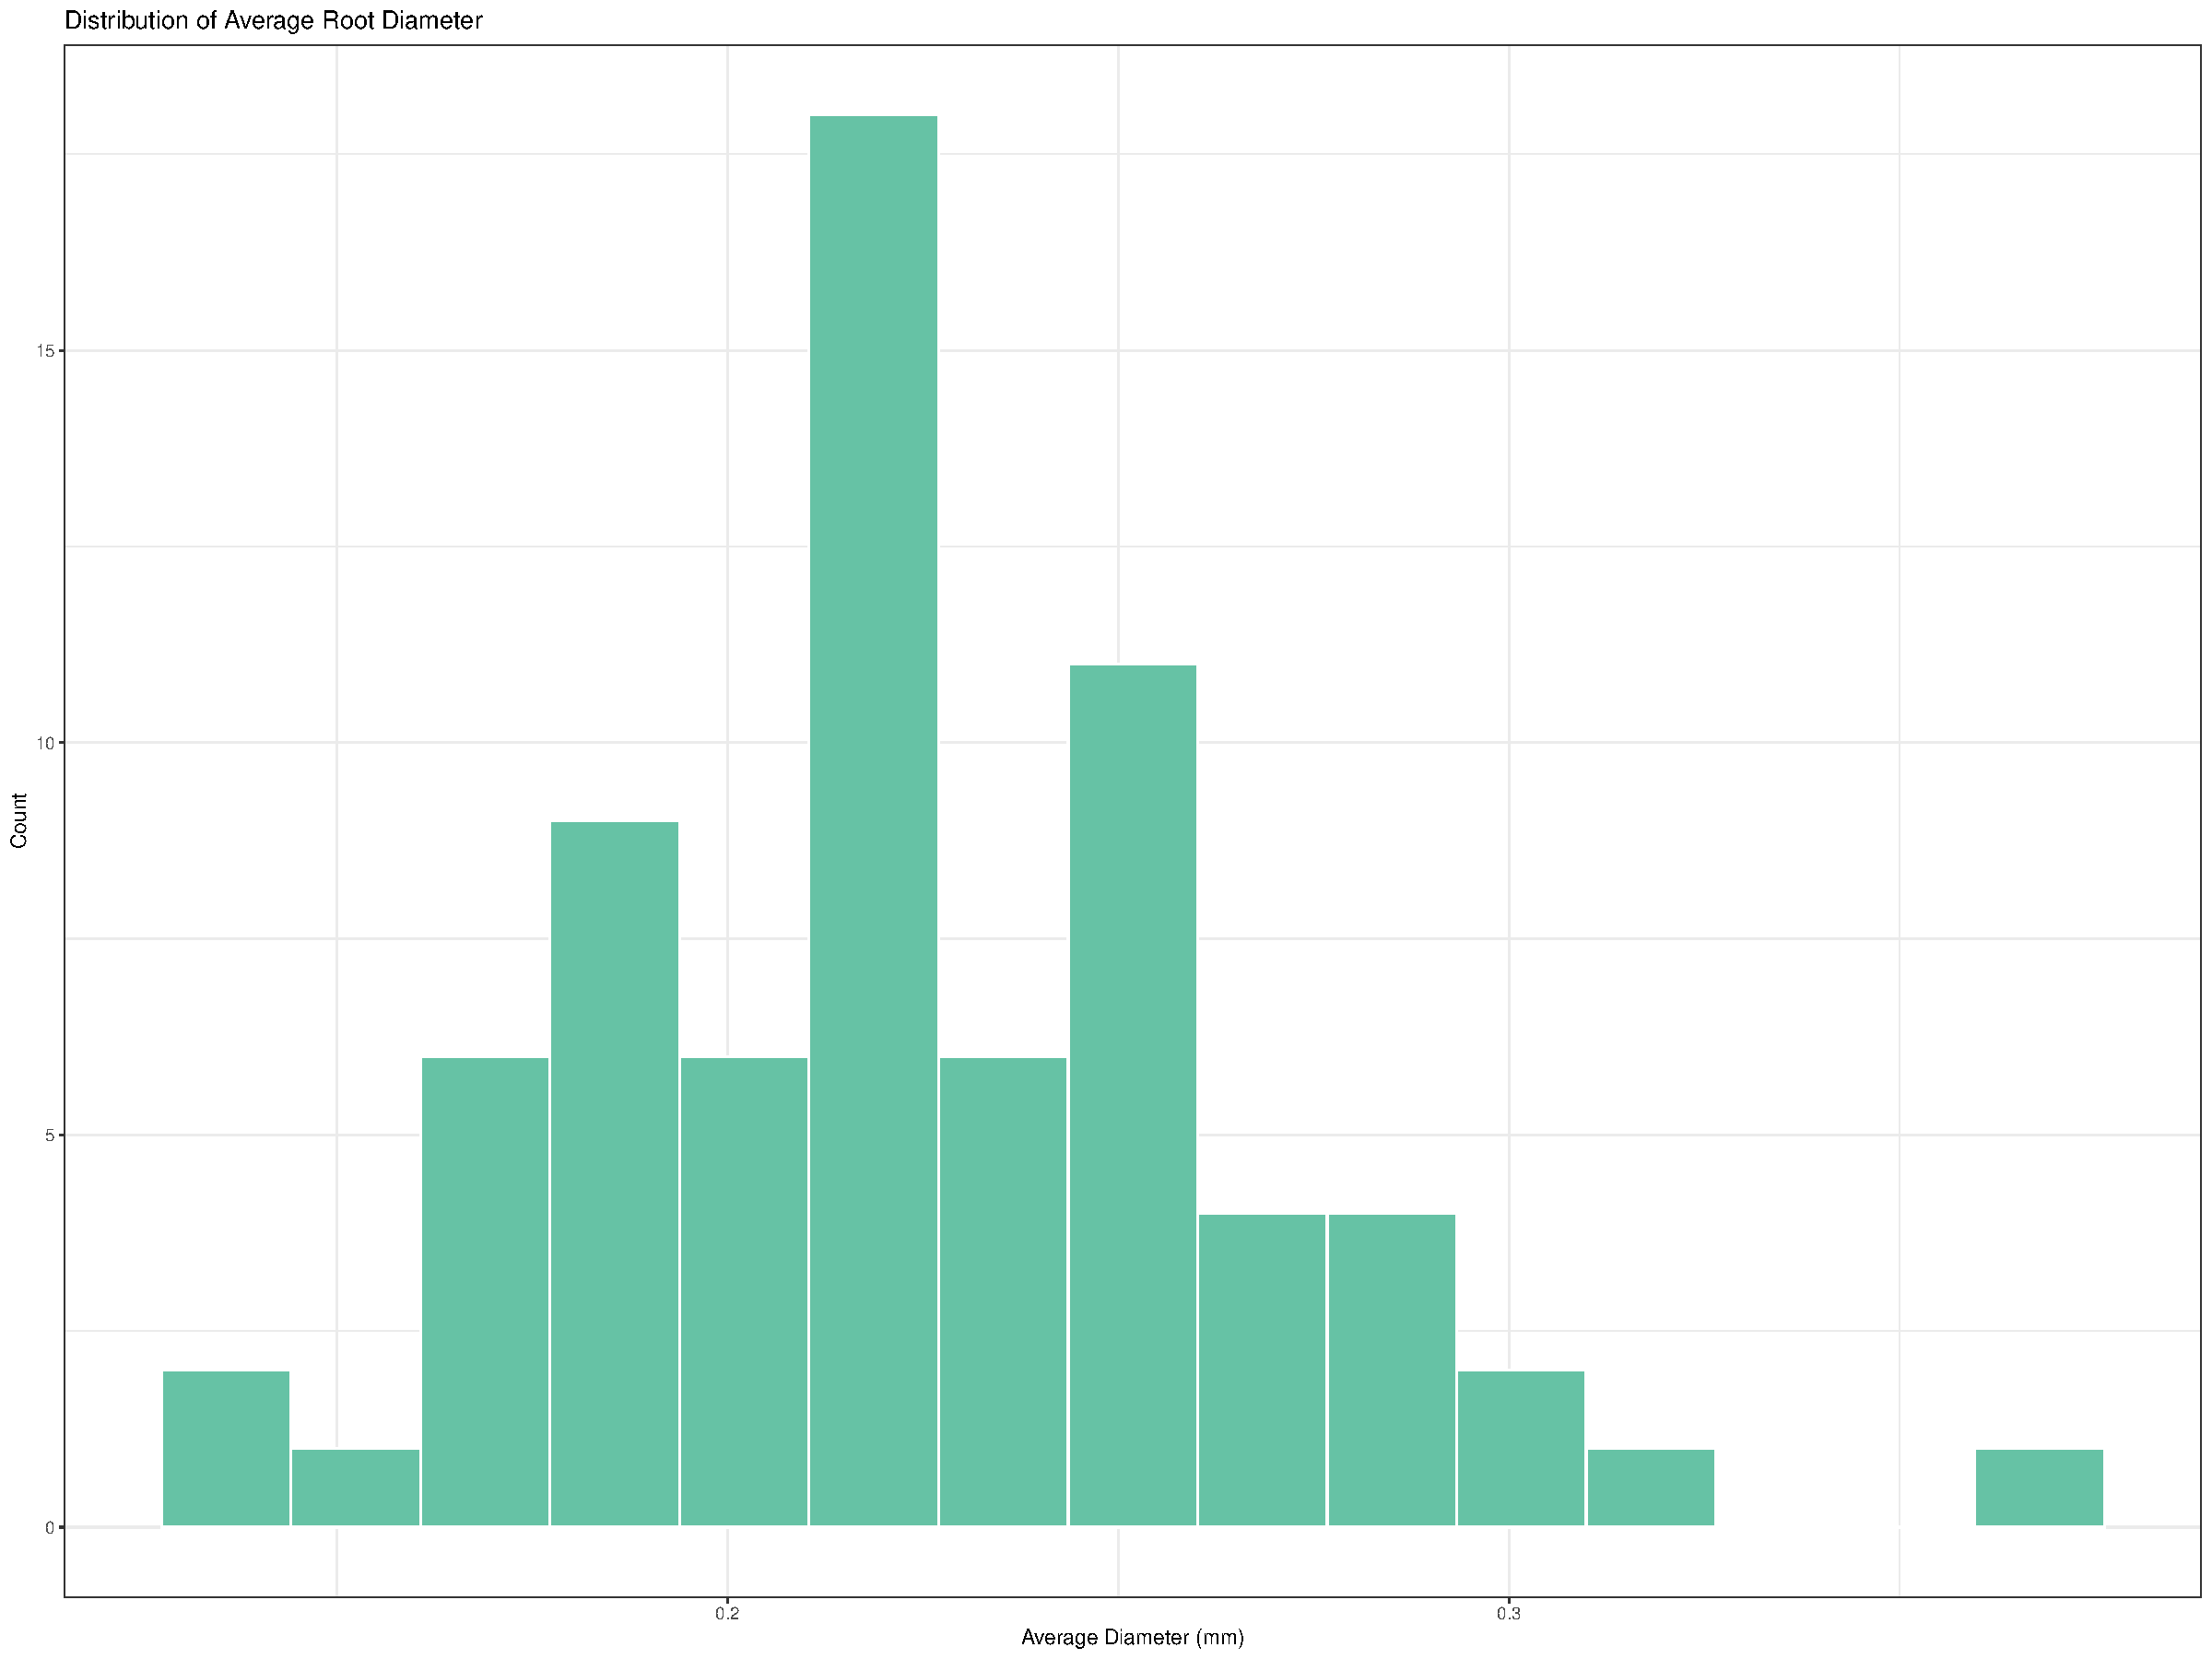
\includegraphics[keepaspectratio]{rsa_day1617_agar_files/figure-pdf/unnamed-chunk-4-1.pdf}}

\begin{Shaded}
\begin{Highlighting}[]
\CommentTok{\# ── Original model (Batch/Plate/Seed nested shorthand) ───────}
\CommentTok{\# R expands this into THREE separate variance components:}
\CommentTok{\# (1|Batch) + (1|Batch:Plate) + (1|Batch:Plate:Seed)}

\NormalTok{diam\_tmb\_full }\OtherTok{\textless{}{-}} \FunctionTok{glmmTMB}\NormalTok{(}
\NormalTok{  Average.Diameter.mm }\SpecialCharTok{\textasciitilde{}}\NormalTok{ Genotype }\SpecialCharTok{+}\NormalTok{ (}\DecValTok{1} \SpecialCharTok{|}\NormalTok{ Batch}\SpecialCharTok{/}\NormalTok{Plate}\SpecialCharTok{/}\NormalTok{Seed),}
  \AttributeTok{data =}\NormalTok{ df, }\AttributeTok{family =} \FunctionTok{gaussian}\NormalTok{()}
\NormalTok{)}

\CommentTok{\# Inspect variance components}
\FunctionTok{VarCorr}\NormalTok{(diam\_tmb\_full)}
\end{Highlighting}
\end{Shaded}

\begin{verbatim}

Conditional model:
 Groups           Name        Std.Dev. 
 Seed:Plate:Batch (Intercept) 0.0060112
 Plate:Batch      (Intercept) 0.0085629
 Batch            (Intercept) 0.0199071
 Residual                     0.0326759
\end{verbatim}

\begin{Shaded}
\begin{Highlighting}[]
\FunctionTok{check\_singularity}\NormalTok{(diam\_tmb\_full) }
\end{Highlighting}
\end{Shaded}

\begin{verbatim}
[1] FALSE
\end{verbatim}

\begin{Shaded}
\begin{Highlighting}[]
\CommentTok{\# Because Plate and Batch variances collapse to \textasciitilde{}0, the Hessian}
\CommentTok{\# matrix becomes singular and all SEs are uncomputable:}

\CommentTok{\# ── Fit reduced models for best fit ─────────────────────────────────────────────────}
\NormalTok{diam\_tmb }\OtherTok{\textless{}{-}} \FunctionTok{glmmTMB}\NormalTok{(}
\NormalTok{  Average.Diameter.mm }\SpecialCharTok{\textasciitilde{}}\NormalTok{ Genotype }\SpecialCharTok{+}\NormalTok{ (}\DecValTok{1} \SpecialCharTok{|}\NormalTok{ Batch}\SpecialCharTok{/}\NormalTok{Plate),}
  \AttributeTok{data =}\NormalTok{ df, }\AttributeTok{family =} \FunctionTok{gaussian}\NormalTok{()}
\NormalTok{)}

\FunctionTok{VarCorr}\NormalTok{(diam\_tmb)}
\end{Highlighting}
\end{Shaded}

\begin{verbatim}

Conditional model:
 Groups      Name        Std.Dev. 
 Plate:Batch (Intercept) 0.0096165
 Batch       (Intercept) 0.0199956
 Residual                0.0329761
\end{verbatim}

\begin{Shaded}
\begin{Highlighting}[]
\FunctionTok{check\_singularity}\NormalTok{(diam\_tmb) }
\end{Highlighting}
\end{Shaded}

\begin{verbatim}
[1] FALSE
\end{verbatim}

\begin{Shaded}
\begin{Highlighting}[]
\CommentTok{\# ── Assumption checks ─────────────────────────────────────────}
\NormalTok{sim\_res }\OtherTok{\textless{}{-}} \FunctionTok{simulateResiduals}\NormalTok{(diam\_tmb, }\AttributeTok{n =} \DecValTok{1000}\NormalTok{)}
\FunctionTok{plot}\NormalTok{(sim\_res)                                  }\CommentTok{\# QQ + residuals vs fitted}
\end{Highlighting}
\end{Shaded}

\pandocbounded{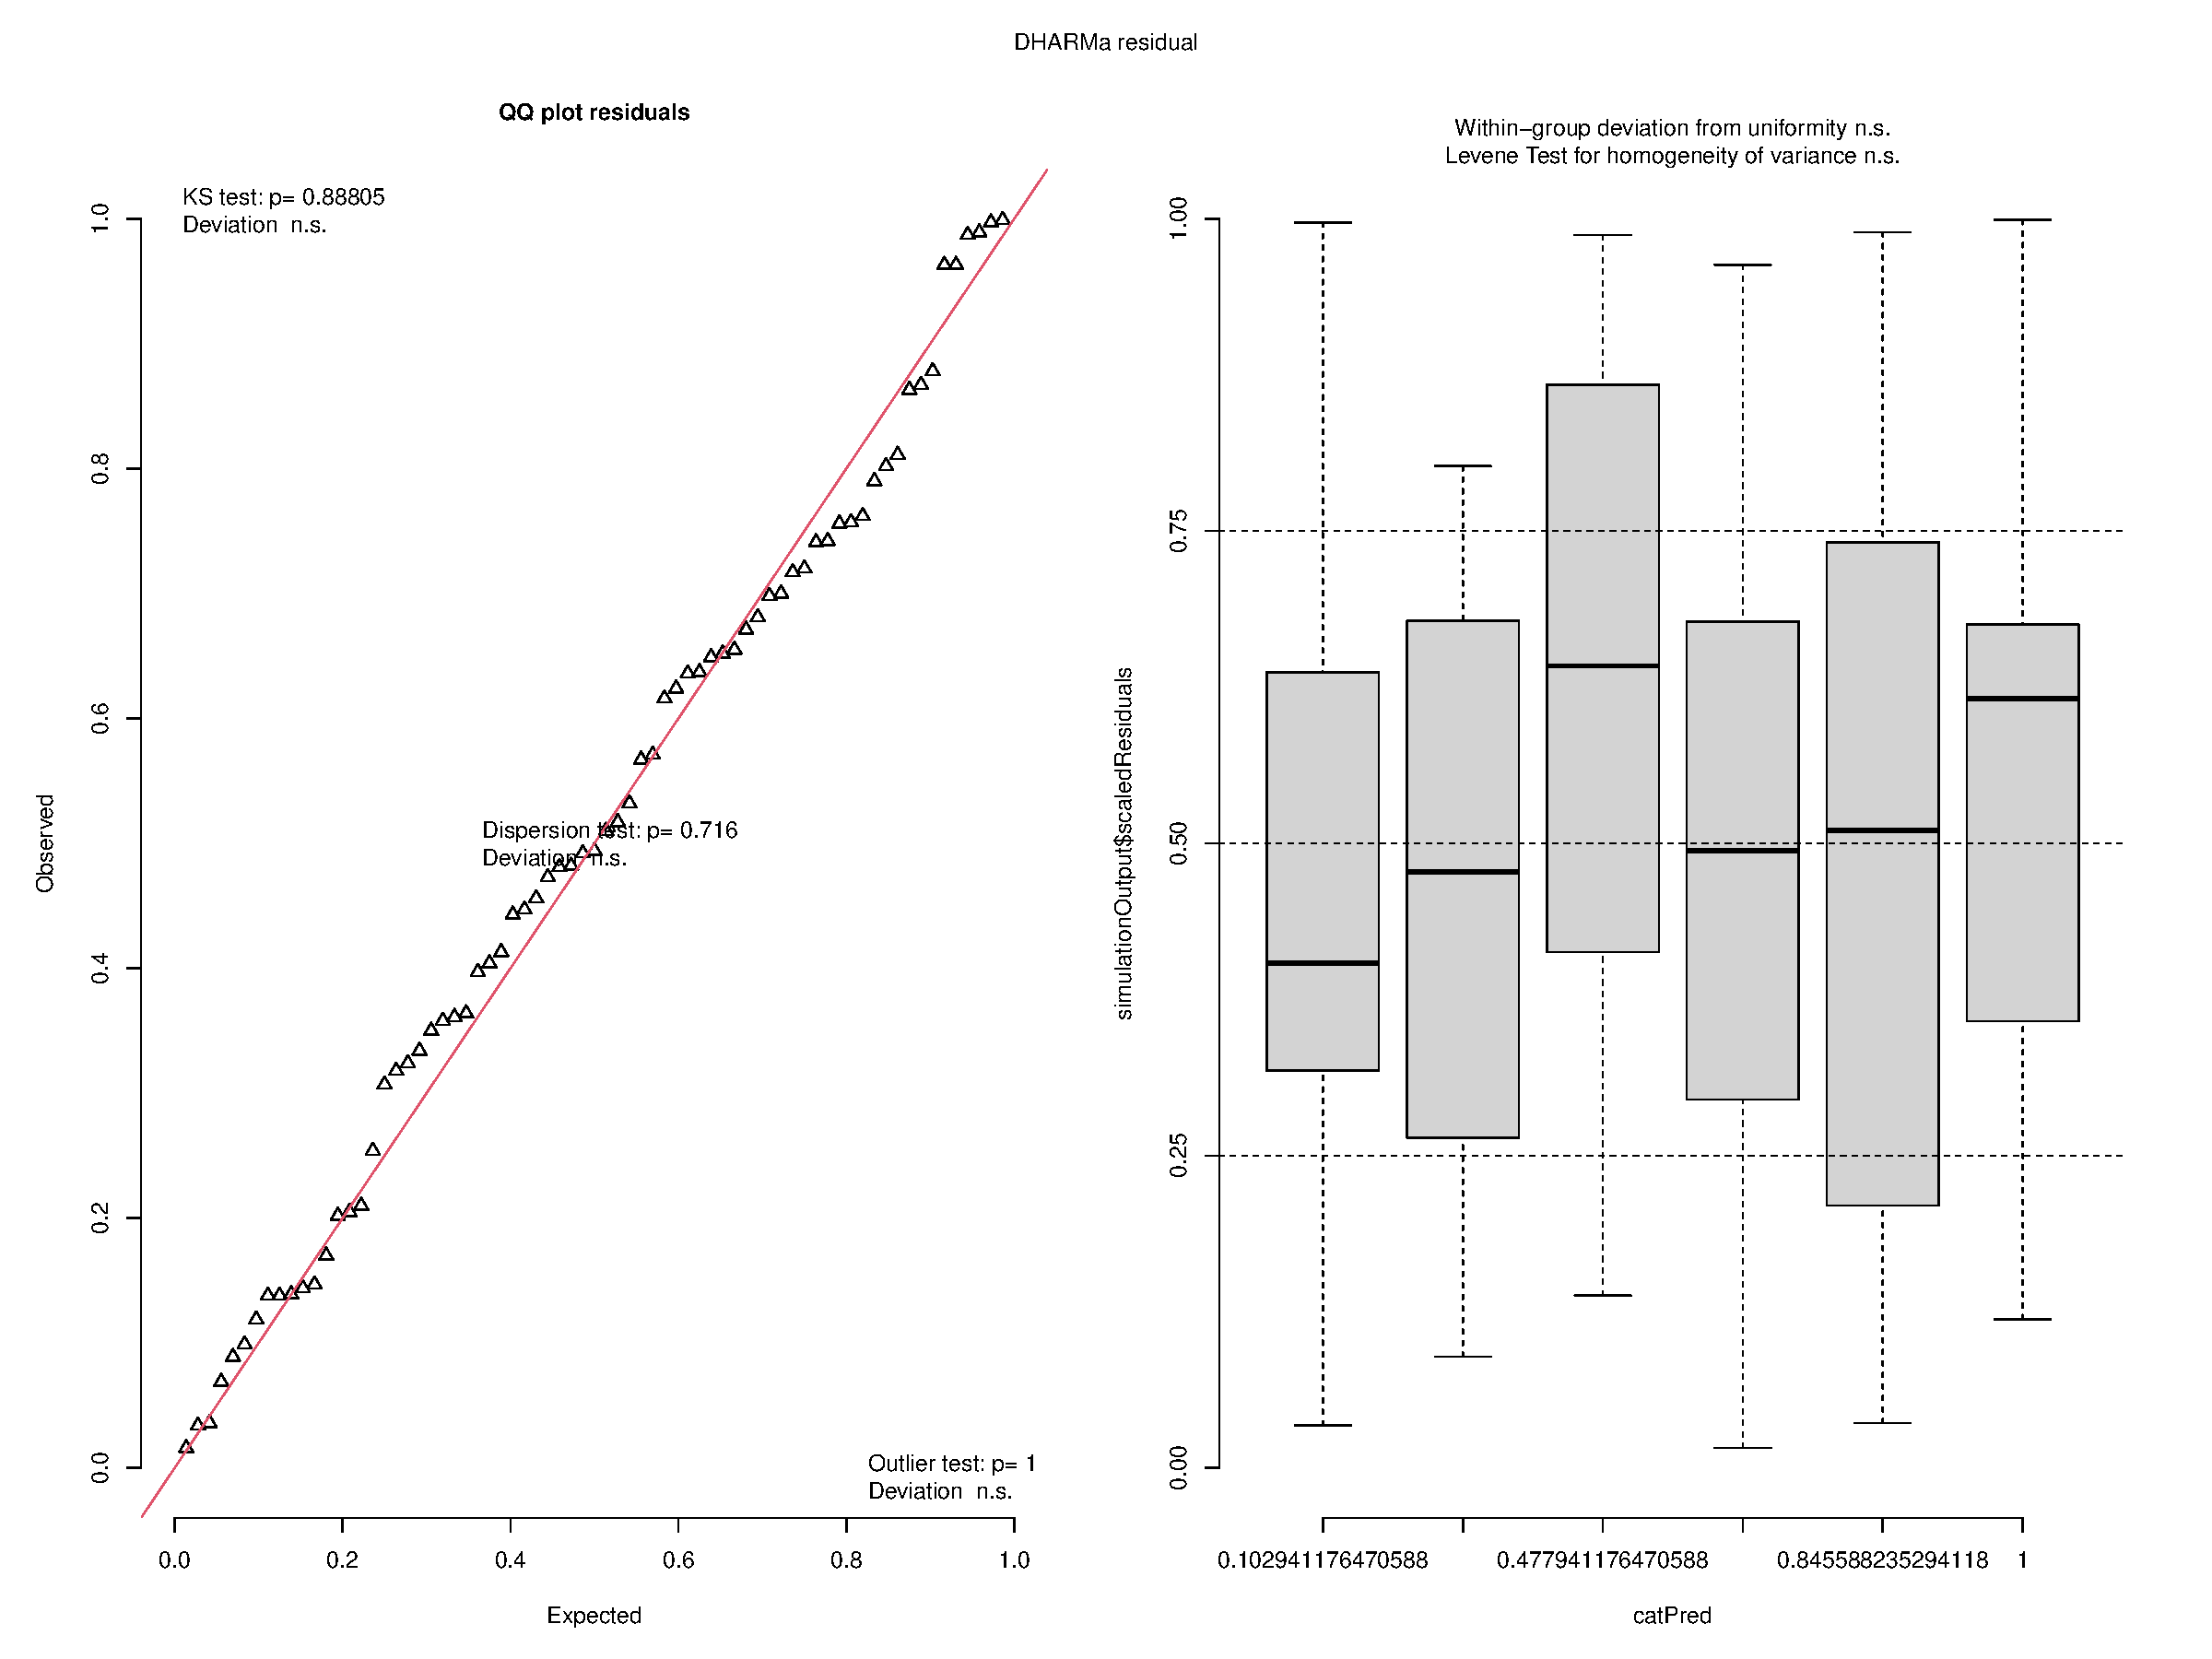
\includegraphics[keepaspectratio]{rsa_day1617_agar_files/figure-pdf/unnamed-chunk-4-2.pdf}}

\begin{Shaded}
\begin{Highlighting}[]
\FunctionTok{testUniformity}\NormalTok{(sim\_res)                        }\CommentTok{\# p \textgreater{} 0.05 = Gaussian appropriate}
\end{Highlighting}
\end{Shaded}

\pandocbounded{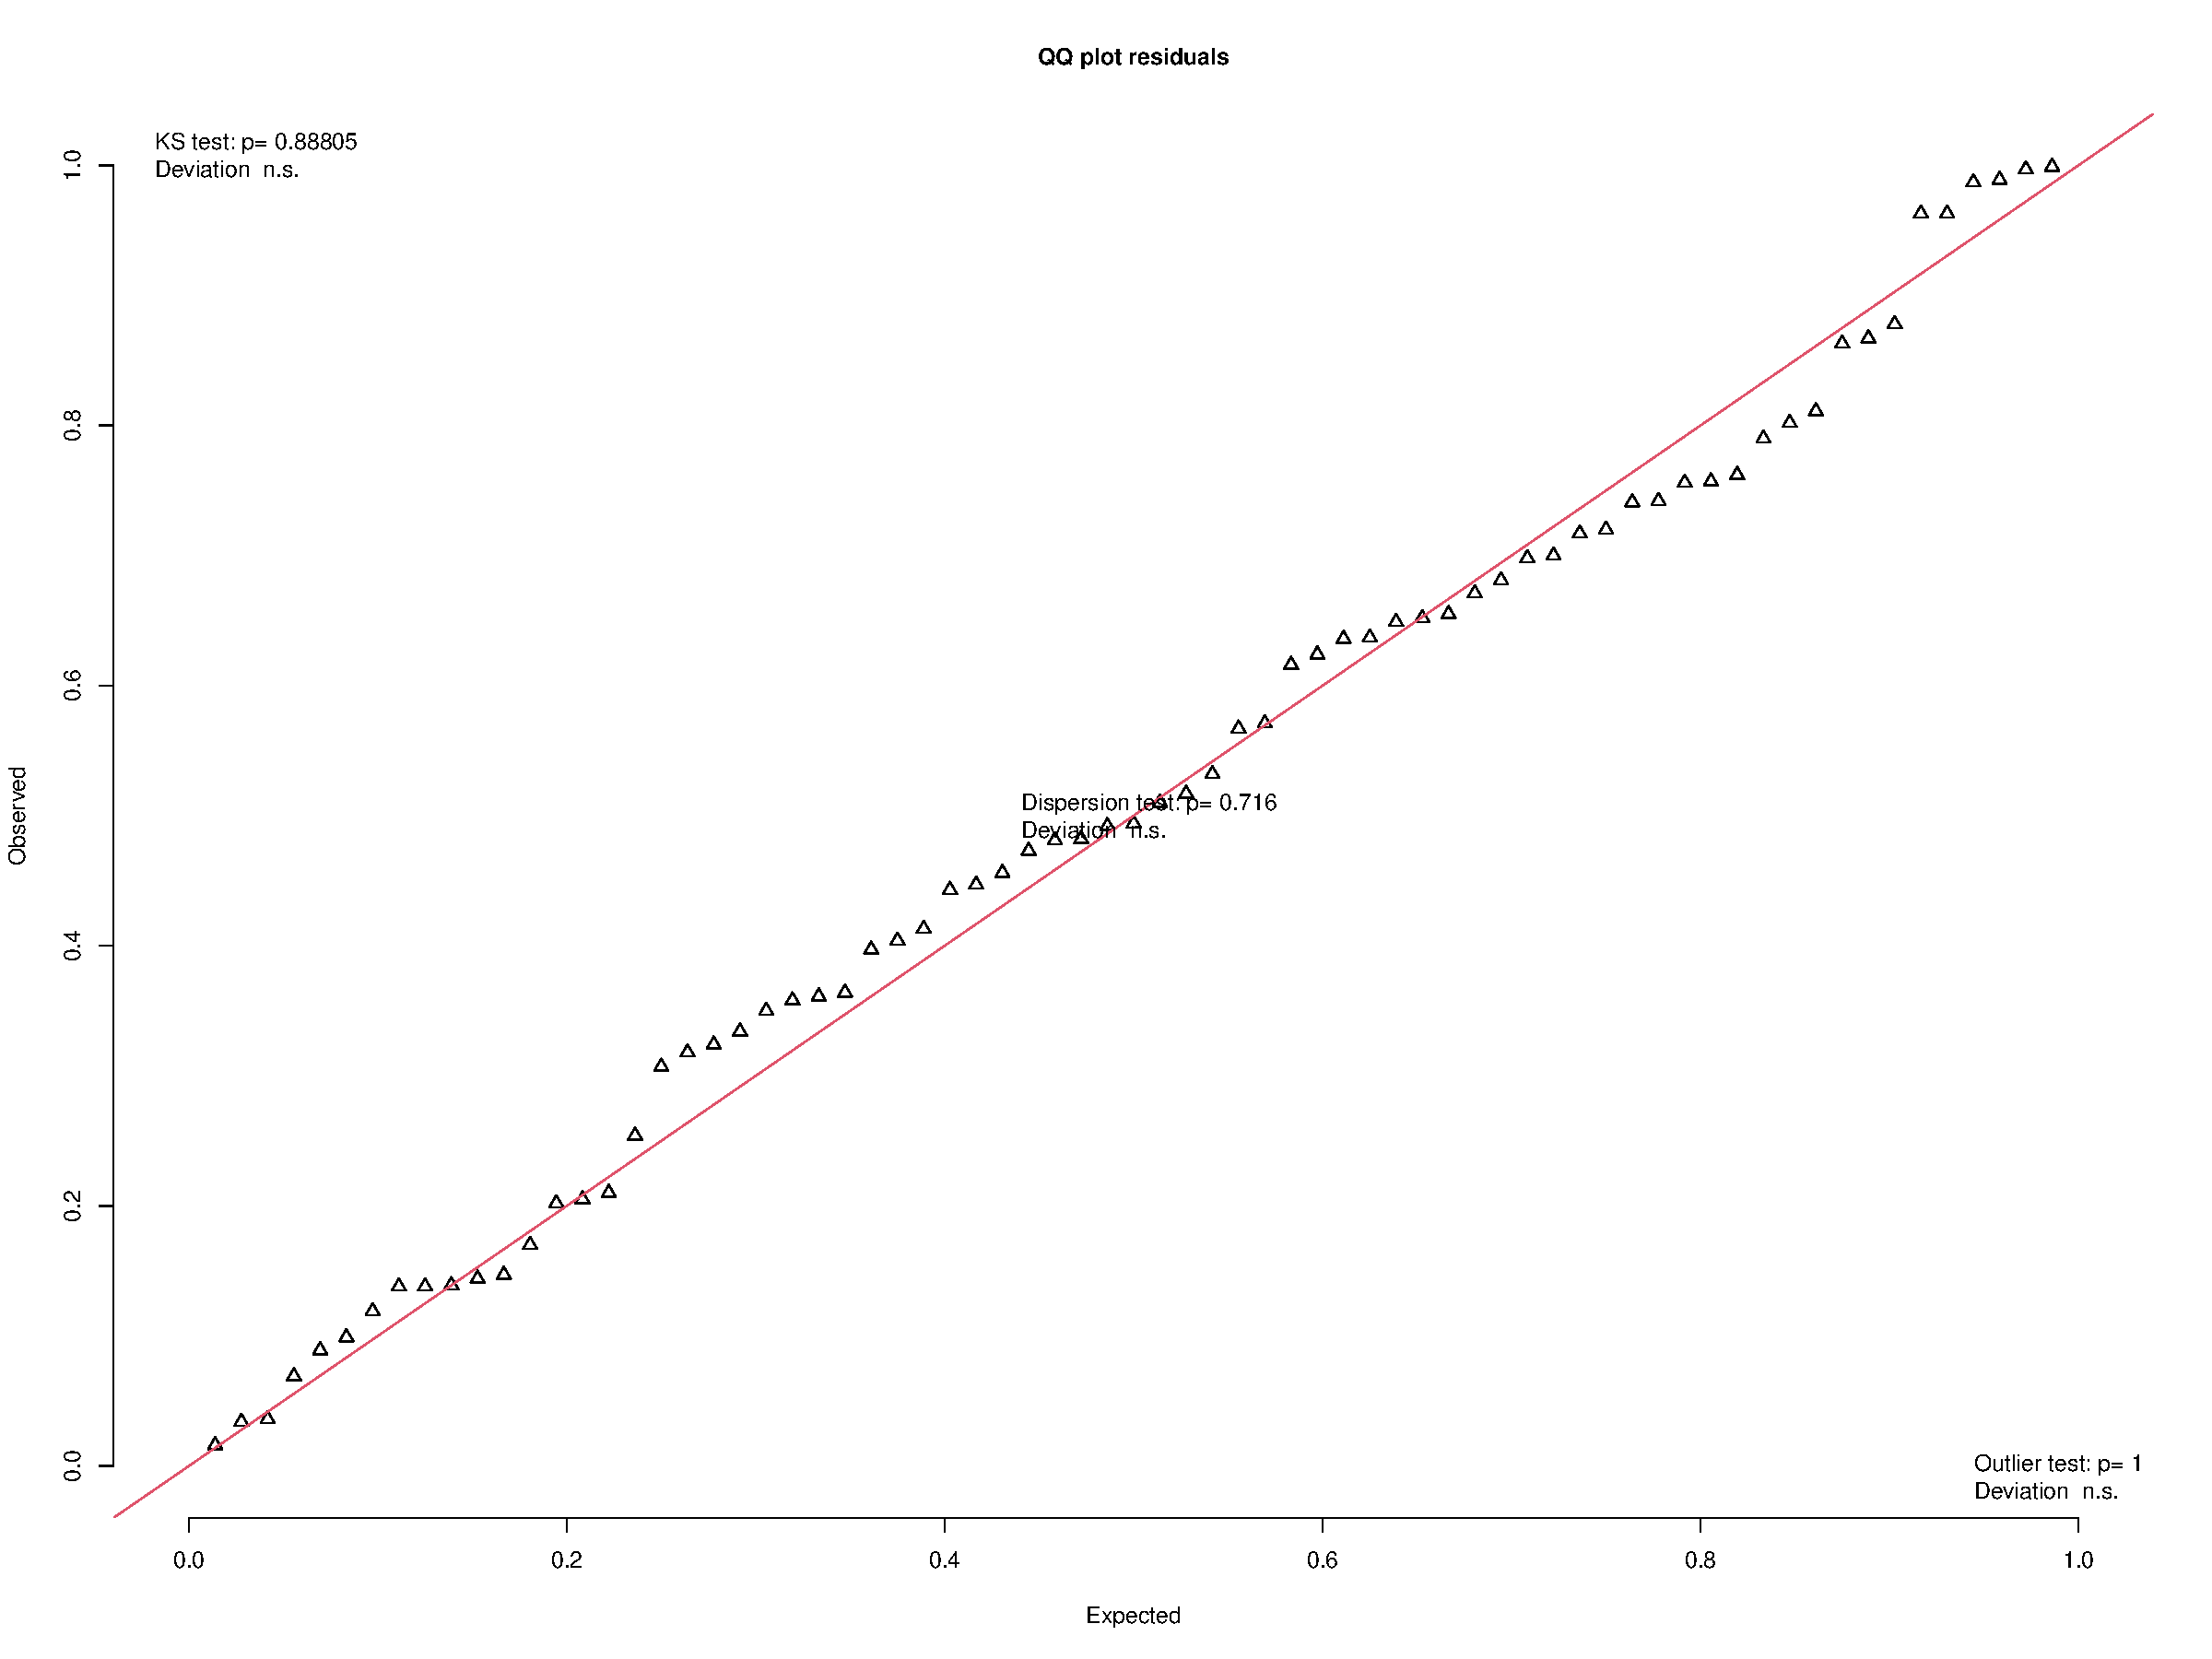
\includegraphics[keepaspectratio]{rsa_day1617_agar_files/figure-pdf/unnamed-chunk-4-3.pdf}}

\begin{verbatim}

    Asymptotic one-sample Kolmogorov-Smirnov test

data:  simulationOutput$scaledResiduals
D = 0.068986, p-value = 0.8881
alternative hypothesis: two-sided
\end{verbatim}

\begin{Shaded}
\begin{Highlighting}[]
\FunctionTok{testDispersion}\NormalTok{(sim\_res)                        }\CommentTok{\# ratio ≈ 1.0 = variance correct}
\end{Highlighting}
\end{Shaded}

\pandocbounded{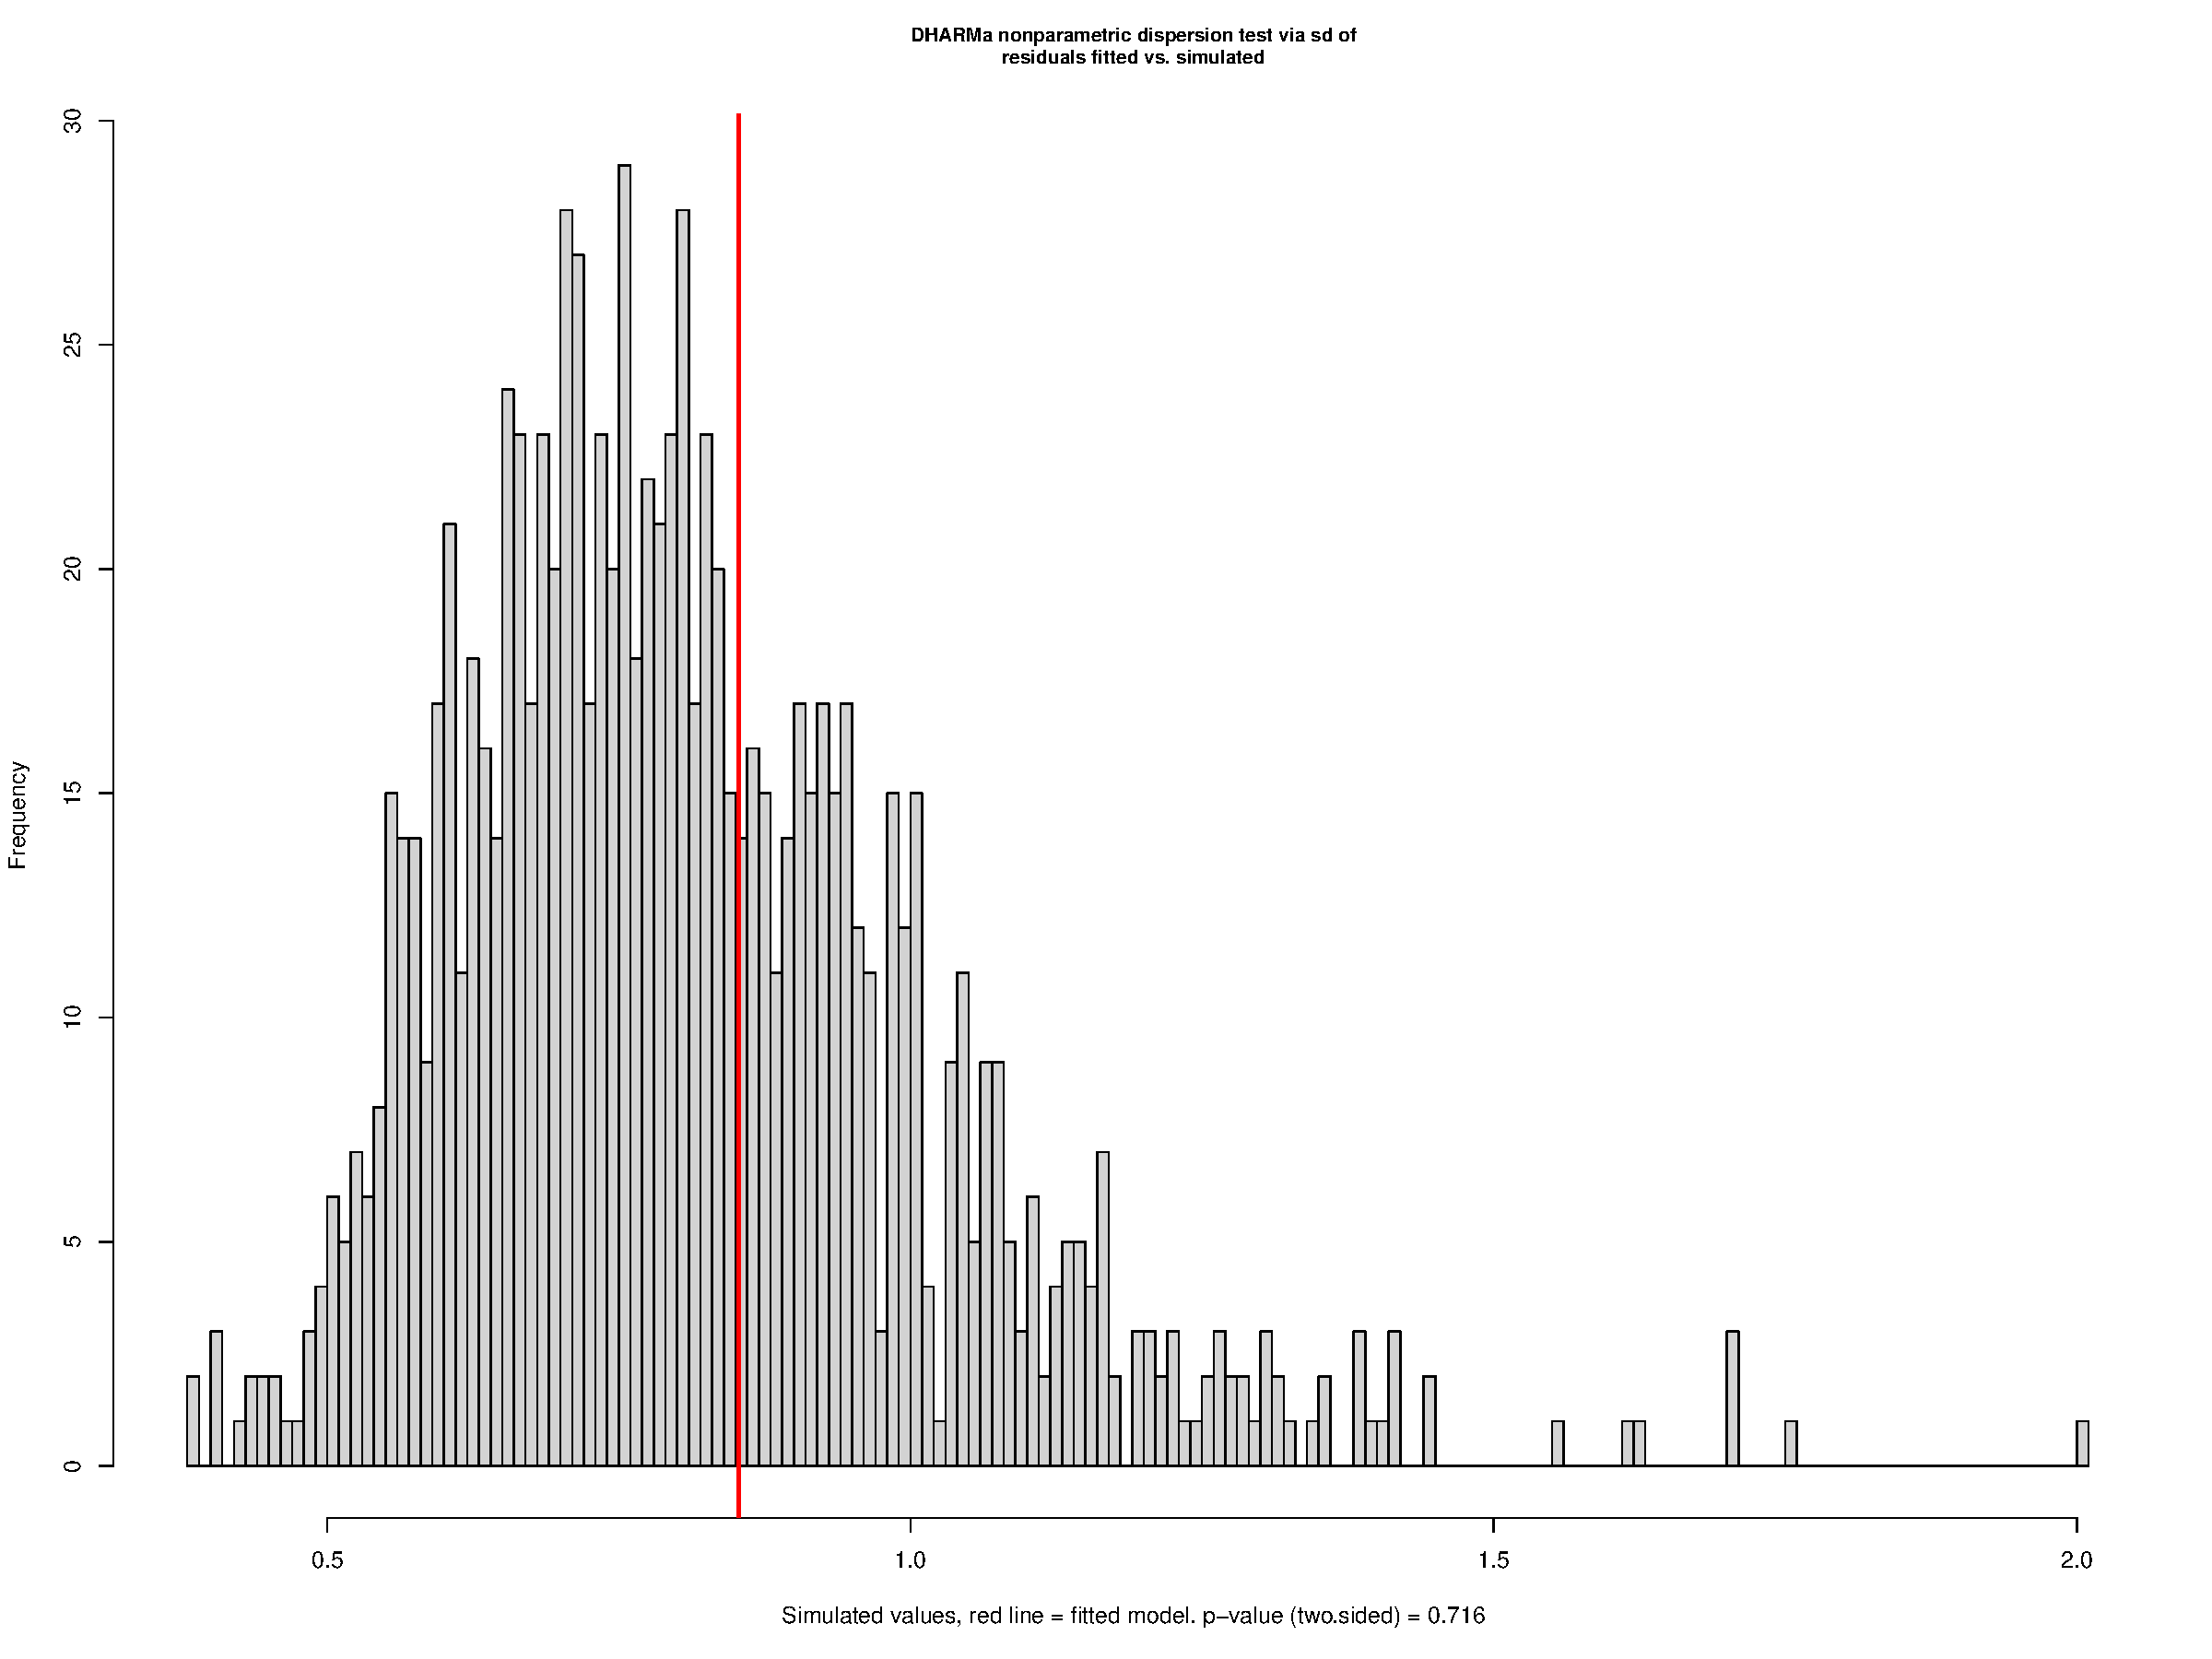
\includegraphics[keepaspectratio]{rsa_day1617_agar_files/figure-pdf/unnamed-chunk-4-4.pdf}}

\begin{verbatim}

    DHARMa nonparametric dispersion test via sd of residuals fitted vs.
    simulated

data:  simulationOutput
dispersion = 1.0482, p-value = 0.716
alternative hypothesis: two.sided
\end{verbatim}

\begin{Shaded}
\begin{Highlighting}[]
\FunctionTok{plotResiduals}\NormalTok{(sim\_res, }\AttributeTok{form =}\NormalTok{ df}\SpecialCharTok{$}\NormalTok{Genotype)     }\CommentTok{\# no patterns per genotype}
\end{Highlighting}
\end{Shaded}

\pandocbounded{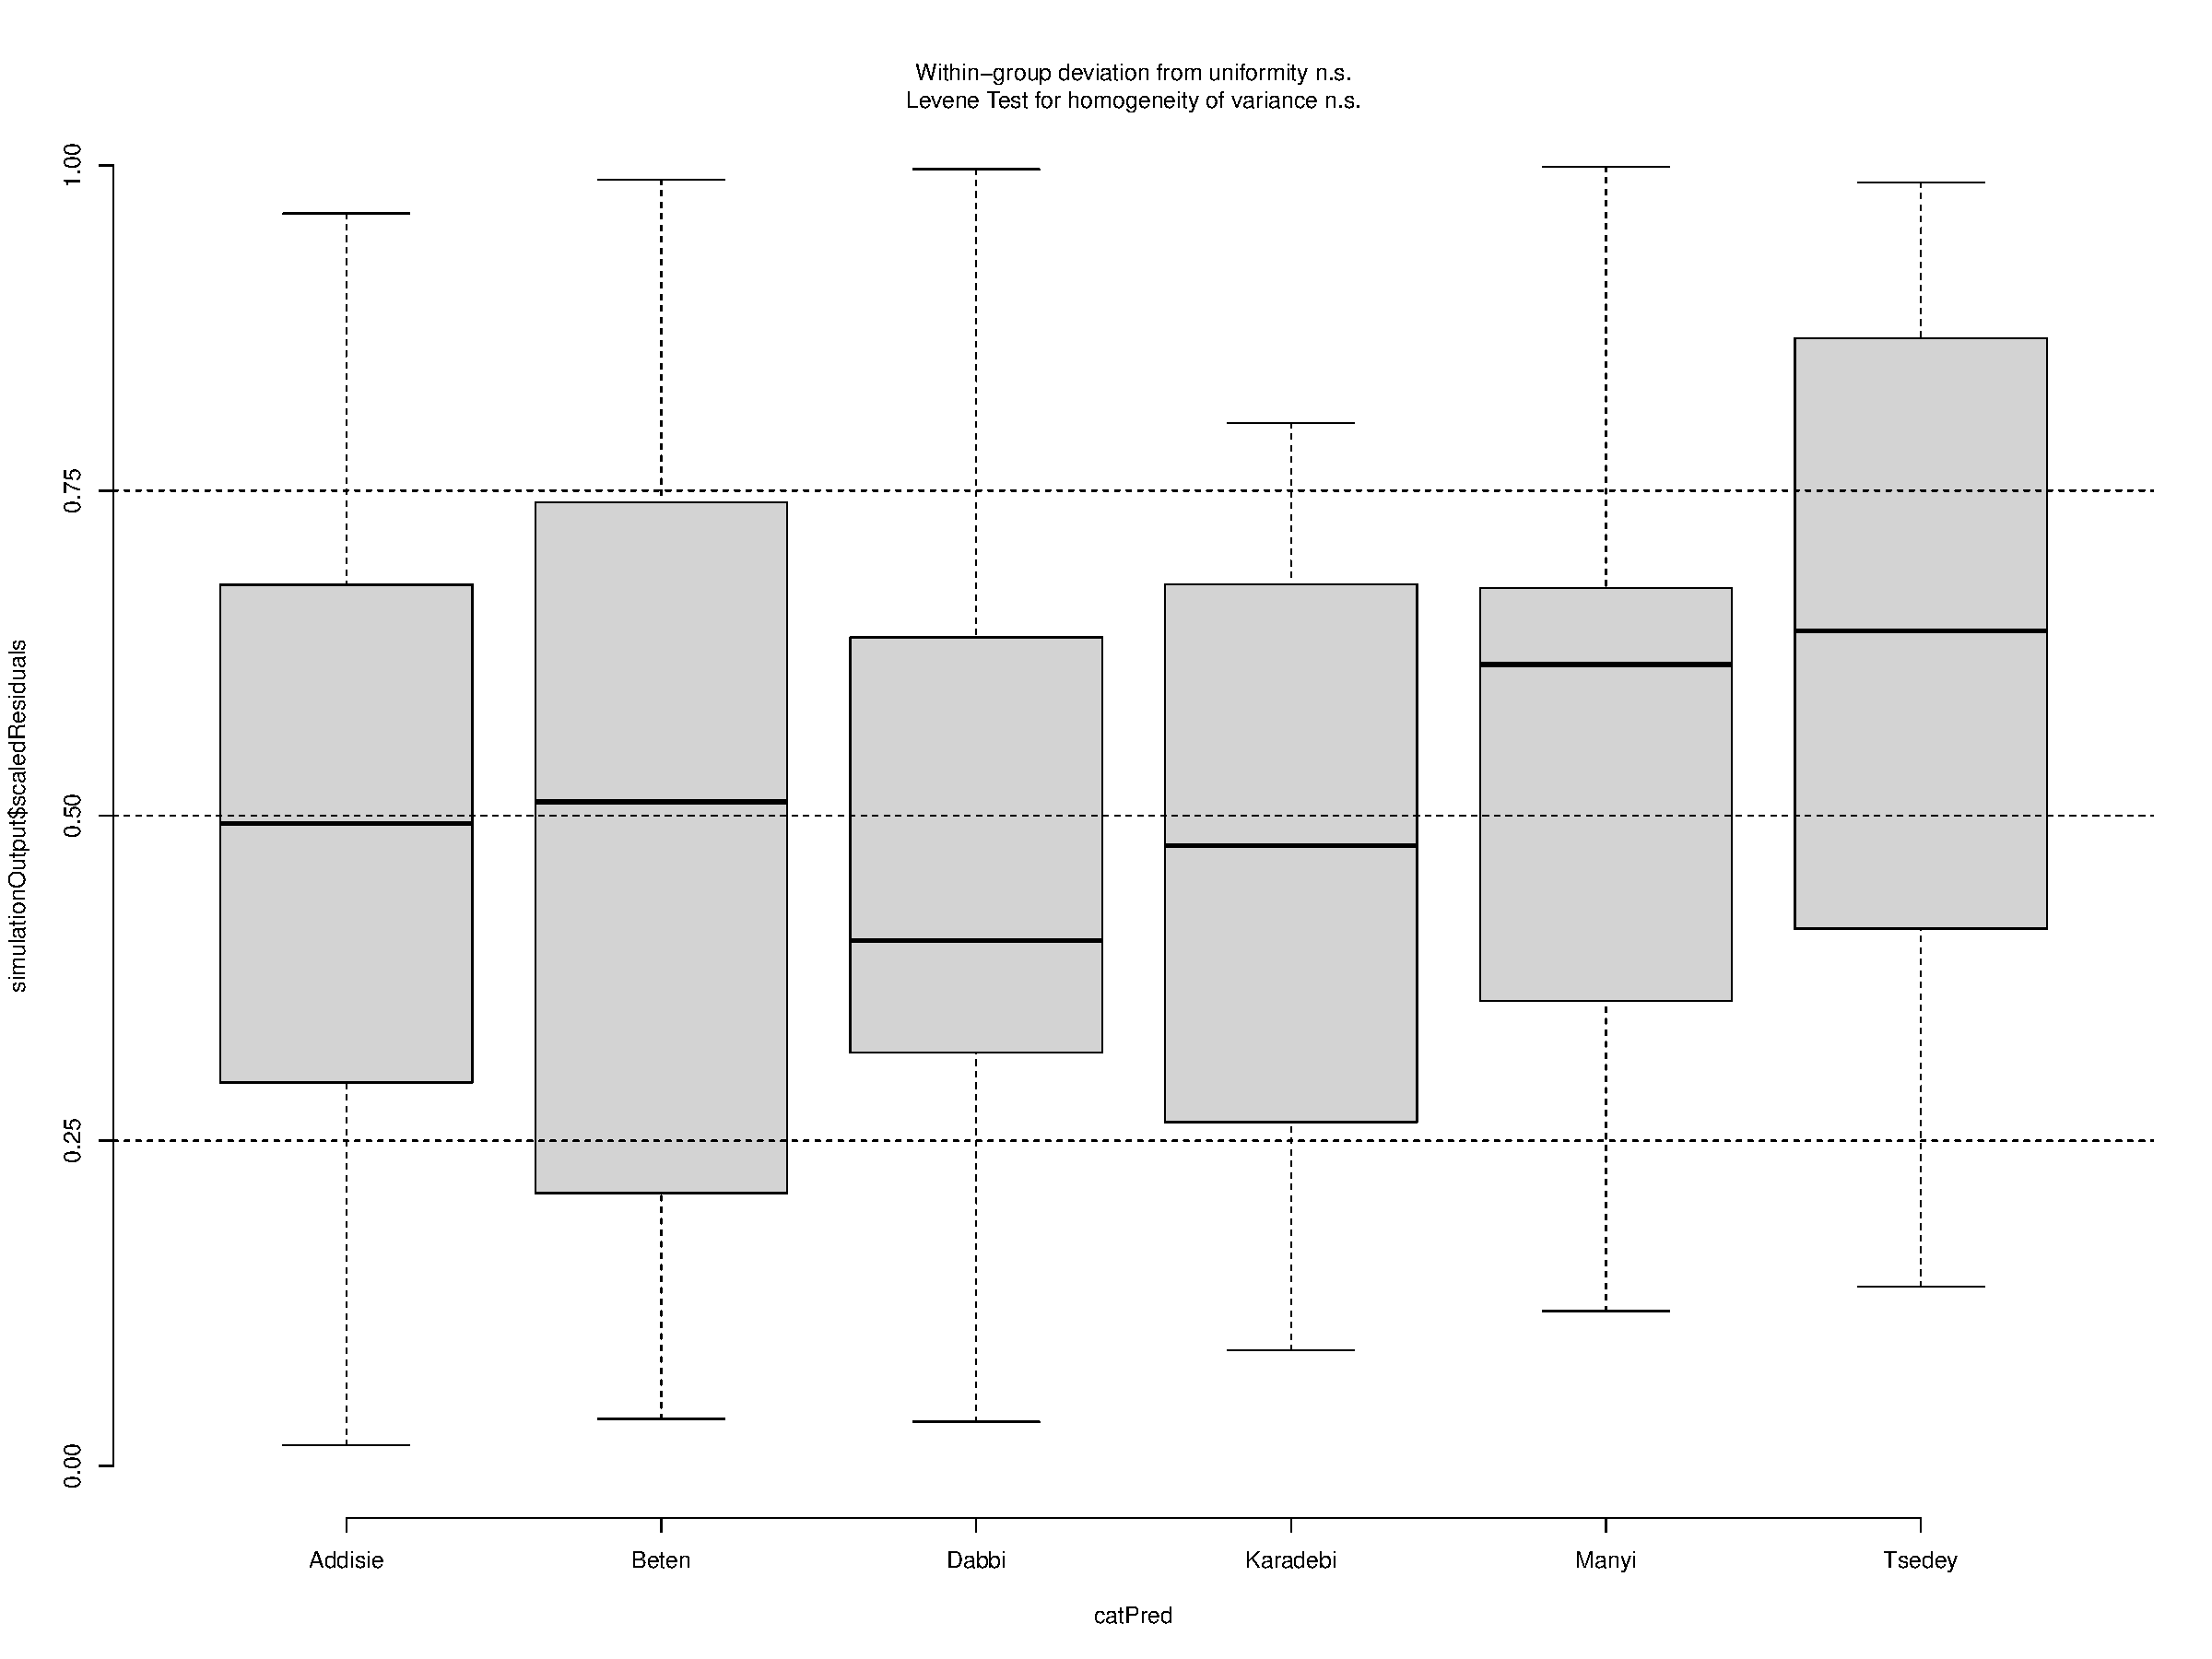
\includegraphics[keepaspectratio]{rsa_day1617_agar_files/figure-pdf/unnamed-chunk-4-5.pdf}}

\begin{Shaded}
\begin{Highlighting}[]
\CommentTok{\# residual fits are all good so happy to continue with this model }

\CommentTok{\# ── Test overall Genotype effect ──────────────────────────────}
\NormalTok{car}\SpecialCharTok{::}\FunctionTok{Anova}\NormalTok{(diam\_tmb, }\AttributeTok{type =} \StringTok{"III"}\NormalTok{)}
\end{Highlighting}
\end{Shaded}

\begin{verbatim}
Analysis of Deviance Table (Type III Wald chisquare tests)

Response: Average.Diameter.mm
              Chisq Df Pr(>Chisq)    
(Intercept) 217.460  1    < 2e-16 ***
Genotype     13.955  5    0.01589 *  
---
Signif. codes:  0 '***' 0.001 '**' 0.01 '*' 0.05 '.' 0.1 ' ' 1
\end{verbatim}

\begin{Shaded}
\begin{Highlighting}[]
\CommentTok{\# ── Pairwise comparisons + CLD ────────────────────────────────}
\NormalTok{emm       }\OtherTok{\textless{}{-}} \FunctionTok{emmeans}\NormalTok{(diam\_tmb, }\SpecialCharTok{\textasciitilde{}}\NormalTok{ Genotype)}
\FunctionTok{pairs}\NormalTok{(emm, }\AttributeTok{adjust =} \StringTok{"sidak"}\NormalTok{)}
\end{Highlighting}
\end{Shaded}

\begin{verbatim}
 contrast            estimate     SE  df z.ratio p.value
 Addisie - Beten    -0.005560 0.0137 Inf  -0.406  1.0000
 Addisie - Dabbi     0.014039 0.0156 Inf   0.898  0.9990
 Addisie - Karadebi  0.003538 0.0154 Inf   0.229  1.0000
 Addisie - Manyi    -0.043690 0.0181 Inf  -2.416  0.2113
 Addisie - Tsedey    0.003426 0.0153 Inf   0.225  1.0000
 Beten - Dabbi       0.019599 0.0148 Inf   1.326  0.9533
 Beten - Karadebi    0.009098 0.0145 Inf   0.627  1.0000
 Beten - Manyi      -0.038130 0.0170 Inf  -2.237  0.3188
 Beten - Tsedey      0.008986 0.0139 Inf   0.646  1.0000
 Dabbi - Karadebi   -0.010501 0.0140 Inf  -0.748  0.9999
 Dabbi - Manyi      -0.057729 0.0165 Inf  -3.499  0.0070
 Dabbi - Tsedey     -0.010613 0.0154 Inf  -0.690  1.0000
 Karadebi - Manyi   -0.047228 0.0164 Inf  -2.876  0.0587
 Karadebi - Tsedey  -0.000112 0.0154 Inf  -0.007  1.0000
 Manyi - Tsedey      0.047116 0.0166 Inf   2.838  0.0660

P value adjustment: sidak method for 15 tests 
\end{verbatim}

\begin{Shaded}
\begin{Highlighting}[]
\NormalTok{cld\_df }\OtherTok{\textless{}{-}} \FunctionTok{as.data.frame}\NormalTok{(}\FunctionTok{cld}\NormalTok{(emm, }\AttributeTok{adjust =} \StringTok{"sidak"}\NormalTok{,}
                             \AttributeTok{Letters =}\NormalTok{ letters, }\AttributeTok{alpha =} \FloatTok{0.05}\NormalTok{)) }\SpecialCharTok{\%\textgreater{}\%}
  \FunctionTok{mutate}\NormalTok{(}\AttributeTok{.group =} \FunctionTok{trimws}\NormalTok{(.group))}


\CommentTok{\# Cohen\textquotesingle{}s d = difference in means / pooled SD}
\CommentTok{\# Interpretation: 0.2 = small, 0.5 = medium, 0.8 = large}

\NormalTok{emm\_diam }\OtherTok{\textless{}{-}} \FunctionTok{emmeans}\NormalTok{(diam\_tmb, }\SpecialCharTok{\textasciitilde{}}\NormalTok{ Genotype)}

\NormalTok{eff\_diam }\OtherTok{\textless{}{-}} \FunctionTok{eff\_size}\NormalTok{(}
\NormalTok{  emm\_diam,}
  \AttributeTok{sigma =} \FunctionTok{sigma}\NormalTok{(diam\_tmb),   }\CommentTok{\# residual SD from model}
  \AttributeTok{edf   =} \FunctionTok{df.residual}\NormalTok{(diam\_tmb)}
\NormalTok{)}
\FunctionTok{print}\NormalTok{(eff\_diam)}
\end{Highlighting}
\end{Shaded}

\begin{verbatim}
 contrast           effect.size    SE  df asymp.LCL asymp.UCL
 Addisie - Beten       -0.16862 0.416 Inf    -0.983     0.646
 Addisie - Dabbi        0.42573 0.475 Inf    -0.506     1.357
 Addisie - Karadebi     0.10728 0.468 Inf    -0.810     1.024
 Addisie - Manyi       -1.32491 0.561 Inf    -2.425    -0.225
 Addisie - Tsedey       0.10389 0.463 Inf    -0.803     1.011
 Beten - Dabbi          0.59435 0.451 Inf    -0.290     1.479
 Beten - Karadebi       0.27591 0.440 Inf    -0.587     1.139
 Beten - Manyi         -1.15629 0.527 Inf    -2.189    -0.123
 Beten - Tsedey         0.27251 0.423 Inf    -0.556     1.101
 Dabbi - Karadebi      -0.31844 0.427 Inf    -1.155     0.518
 Dabbi - Manyi         -1.75064 0.524 Inf    -2.778    -0.723
 Dabbi - Tsedey        -0.32184 0.467 Inf    -1.237     0.594
 Karadebi - Manyi      -1.43220 0.514 Inf    -2.440    -0.424
 Karadebi - Tsedey     -0.00339 0.466 Inf    -0.916     0.909
 Manyi - Tsedey         1.42880 0.520 Inf     0.410     2.447

sigma used for effect sizes: 0.03298 
Confidence level used: 0.95 
\end{verbatim}

\begin{Shaded}
\begin{Highlighting}[]
\CommentTok{\# most effect sizes are relatively small}

\CommentTok{\# ── Sample size labels ────────────────────────────────────────}
\NormalTok{n\_df }\OtherTok{\textless{}{-}}\NormalTok{ df }\SpecialCharTok{\%\textgreater{}\%}
  \FunctionTok{count}\NormalTok{(Genotype) }\SpecialCharTok{\%\textgreater{}\%}
  \FunctionTok{mutate}\NormalTok{(}\AttributeTok{label =} \FunctionTok{paste0}\NormalTok{(}\StringTok{"n="}\NormalTok{, n))}

\CommentTok{\# ── CLD letter position (above tallest box) ───────────────────}

\NormalTok{y\_ceil }\OtherTok{\textless{}{-}} \FunctionTok{max}\NormalTok{(df}\SpecialCharTok{$}\NormalTok{Average.Diameter.mm) }\SpecialCharTok{*} \FloatTok{1.2}
\NormalTok{y\_label }\OtherTok{\textless{}{-}}\NormalTok{ y\_ceil }\SpecialCharTok{*} \FloatTok{0.85}

\CommentTok{\# ── Plot 1: Boxplot + jitter (mirrors your template exactly) ──}
\NormalTok{p1 }\OtherTok{\textless{}{-}} \FunctionTok{ggplot}\NormalTok{(df, }\FunctionTok{aes}\NormalTok{(}\AttributeTok{x =}\NormalTok{ Genotype, }\AttributeTok{y =}\NormalTok{ Average.Diameter.mm, }\AttributeTok{fill =}\NormalTok{ Genotype)) }\SpecialCharTok{+}

  \FunctionTok{geom\_boxplot}\NormalTok{(}
    \AttributeTok{alpha         =} \FloatTok{0.7}\NormalTok{,}
    \AttributeTok{outlier.shape =} \ConstantTok{NA}\NormalTok{,}
    \AttributeTok{width         =} \FloatTok{0.5}\NormalTok{,}
    \AttributeTok{colour        =} \StringTok{"black"}\NormalTok{,}
    \AttributeTok{linewidth     =} \FloatTok{0.5}
\NormalTok{  ) }\SpecialCharTok{+}

  \FunctionTok{geom\_jitter}\NormalTok{(}
    \AttributeTok{width  =} \FloatTok{0.15}\NormalTok{,}
    \AttributeTok{size   =} \FloatTok{1.8}\NormalTok{,}
    \AttributeTok{alpha  =} \FloatTok{0.55}\NormalTok{,}
    \AttributeTok{colour =} \StringTok{"black"}
\NormalTok{  ) }\SpecialCharTok{+}

  \FunctionTok{geom\_text}\NormalTok{(}
    \AttributeTok{data        =}\NormalTok{ cld\_df,}
    \FunctionTok{aes}\NormalTok{(}\AttributeTok{x =}\NormalTok{ Genotype, }\AttributeTok{label =}\NormalTok{ .group),}
    \AttributeTok{y           =}\NormalTok{ y\_label,}
    \AttributeTok{inherit.aes =} \ConstantTok{FALSE}\NormalTok{,}
    \AttributeTok{size        =} \DecValTok{8}\NormalTok{,}
    \AttributeTok{fontface    =} \StringTok{"bold"}\NormalTok{,}
    \AttributeTok{colour      =} \StringTok{"grey20"}
\NormalTok{  ) }\SpecialCharTok{+}

  \FunctionTok{geom\_text}\NormalTok{(}
    \AttributeTok{data        =}\NormalTok{ n\_df,}
    \FunctionTok{aes}\NormalTok{(}\AttributeTok{x =}\NormalTok{ Genotype, }\AttributeTok{label =}\NormalTok{ label),}
    \AttributeTok{y           =} \SpecialCharTok{{-}}\ConstantTok{Inf}\NormalTok{,}
    \AttributeTok{vjust       =} \FloatTok{4.2}\NormalTok{,}
    \AttributeTok{inherit.aes =} \ConstantTok{FALSE}\NormalTok{,}
    \AttributeTok{size        =} \DecValTok{6}\NormalTok{,}
    \AttributeTok{colour      =} \StringTok{"grey40"}
\NormalTok{  ) }\SpecialCharTok{+}

  \FunctionTok{scale\_fill\_brewer}\NormalTok{(}\AttributeTok{palette =} \StringTok{"Set2"}\NormalTok{) }\SpecialCharTok{+}

  \FunctionTok{labs}\NormalTok{(}
    \AttributeTok{x       =} \StringTok{"Genotype"}\NormalTok{,}
    \AttributeTok{y       =} \StringTok{"Average root diameter (mm)"}\NormalTok{,}
    \AttributeTok{caption =} \StringTok{"Shared letters indicate no significant difference (sidak HSD, p \textgreater{} 0.05; glmmTMB, Gaussian)"}
\NormalTok{  ) }\SpecialCharTok{+}

  \FunctionTok{theme\_classic}\NormalTok{(}\AttributeTok{base\_size =} \DecValTok{14}\NormalTok{) }\SpecialCharTok{+}
  \FunctionTok{theme}\NormalTok{(}
    \AttributeTok{legend.position =} \StringTok{"none"}\NormalTok{,}
    \AttributeTok{panel.grid      =} \FunctionTok{element\_blank}\NormalTok{(),}
    \AttributeTok{axis.line       =} \FunctionTok{element\_line}\NormalTok{(}\AttributeTok{colour =} \StringTok{"black"}\NormalTok{, }\AttributeTok{linewidth =} \FloatTok{0.6}\NormalTok{),}
    \AttributeTok{axis.ticks      =} \FunctionTok{element\_line}\NormalTok{(}\AttributeTok{colour =} \StringTok{"black"}\NormalTok{, }\AttributeTok{linewidth =} \FloatTok{0.5}\NormalTok{),}
    \AttributeTok{axis.title      =} \FunctionTok{element\_text}\NormalTok{(}\AttributeTok{size =} \DecValTok{26}\NormalTok{, }\AttributeTok{face =} \StringTok{"bold"}\NormalTok{),}
    \AttributeTok{axis.title.x    =} \FunctionTok{element\_text}\NormalTok{(}\AttributeTok{size =} \DecValTok{26}\NormalTok{, }\AttributeTok{face =} \StringTok{"bold"}\NormalTok{, }\AttributeTok{margin =} \FunctionTok{margin}\NormalTok{(}\AttributeTok{t =} \DecValTok{24}\NormalTok{)),}
    \AttributeTok{axis.text       =} \FunctionTok{element\_text}\NormalTok{(}\AttributeTok{size =} \DecValTok{22}\NormalTok{, }\AttributeTok{colour =} \StringTok{"black"}\NormalTok{),}
    \AttributeTok{axis.text.x     =} \FunctionTok{element\_text}\NormalTok{(}\AttributeTok{face =} \StringTok{"italic"}\NormalTok{, }\AttributeTok{margin =} \FunctionTok{margin}\NormalTok{(}\AttributeTok{t =} \DecValTok{15}\NormalTok{)),}
    \AttributeTok{plot.caption    =} \FunctionTok{element\_text}\NormalTok{(}\AttributeTok{size =} \DecValTok{12}\NormalTok{, }\AttributeTok{colour =} \StringTok{"grey40"}\NormalTok{, }\AttributeTok{hjust =} \DecValTok{0}\NormalTok{, }\AttributeTok{margin =} \FunctionTok{margin}\NormalTok{(}\AttributeTok{t =} \DecValTok{10}\NormalTok{)),}
    \AttributeTok{plot.margin     =} \FunctionTok{margin}\NormalTok{(}\AttributeTok{t =} \DecValTok{25}\NormalTok{, }\AttributeTok{r =} \DecValTok{25}\NormalTok{, }\AttributeTok{b =} \DecValTok{25}\NormalTok{, }\AttributeTok{l =} \DecValTok{25}\NormalTok{)}
\NormalTok{  )}


\NormalTok{p1 }\SpecialCharTok{+} \FunctionTok{coord\_cartesian}\NormalTok{(}\AttributeTok{clip =} \StringTok{"off"}\NormalTok{)}
\end{Highlighting}
\end{Shaded}

\pandocbounded{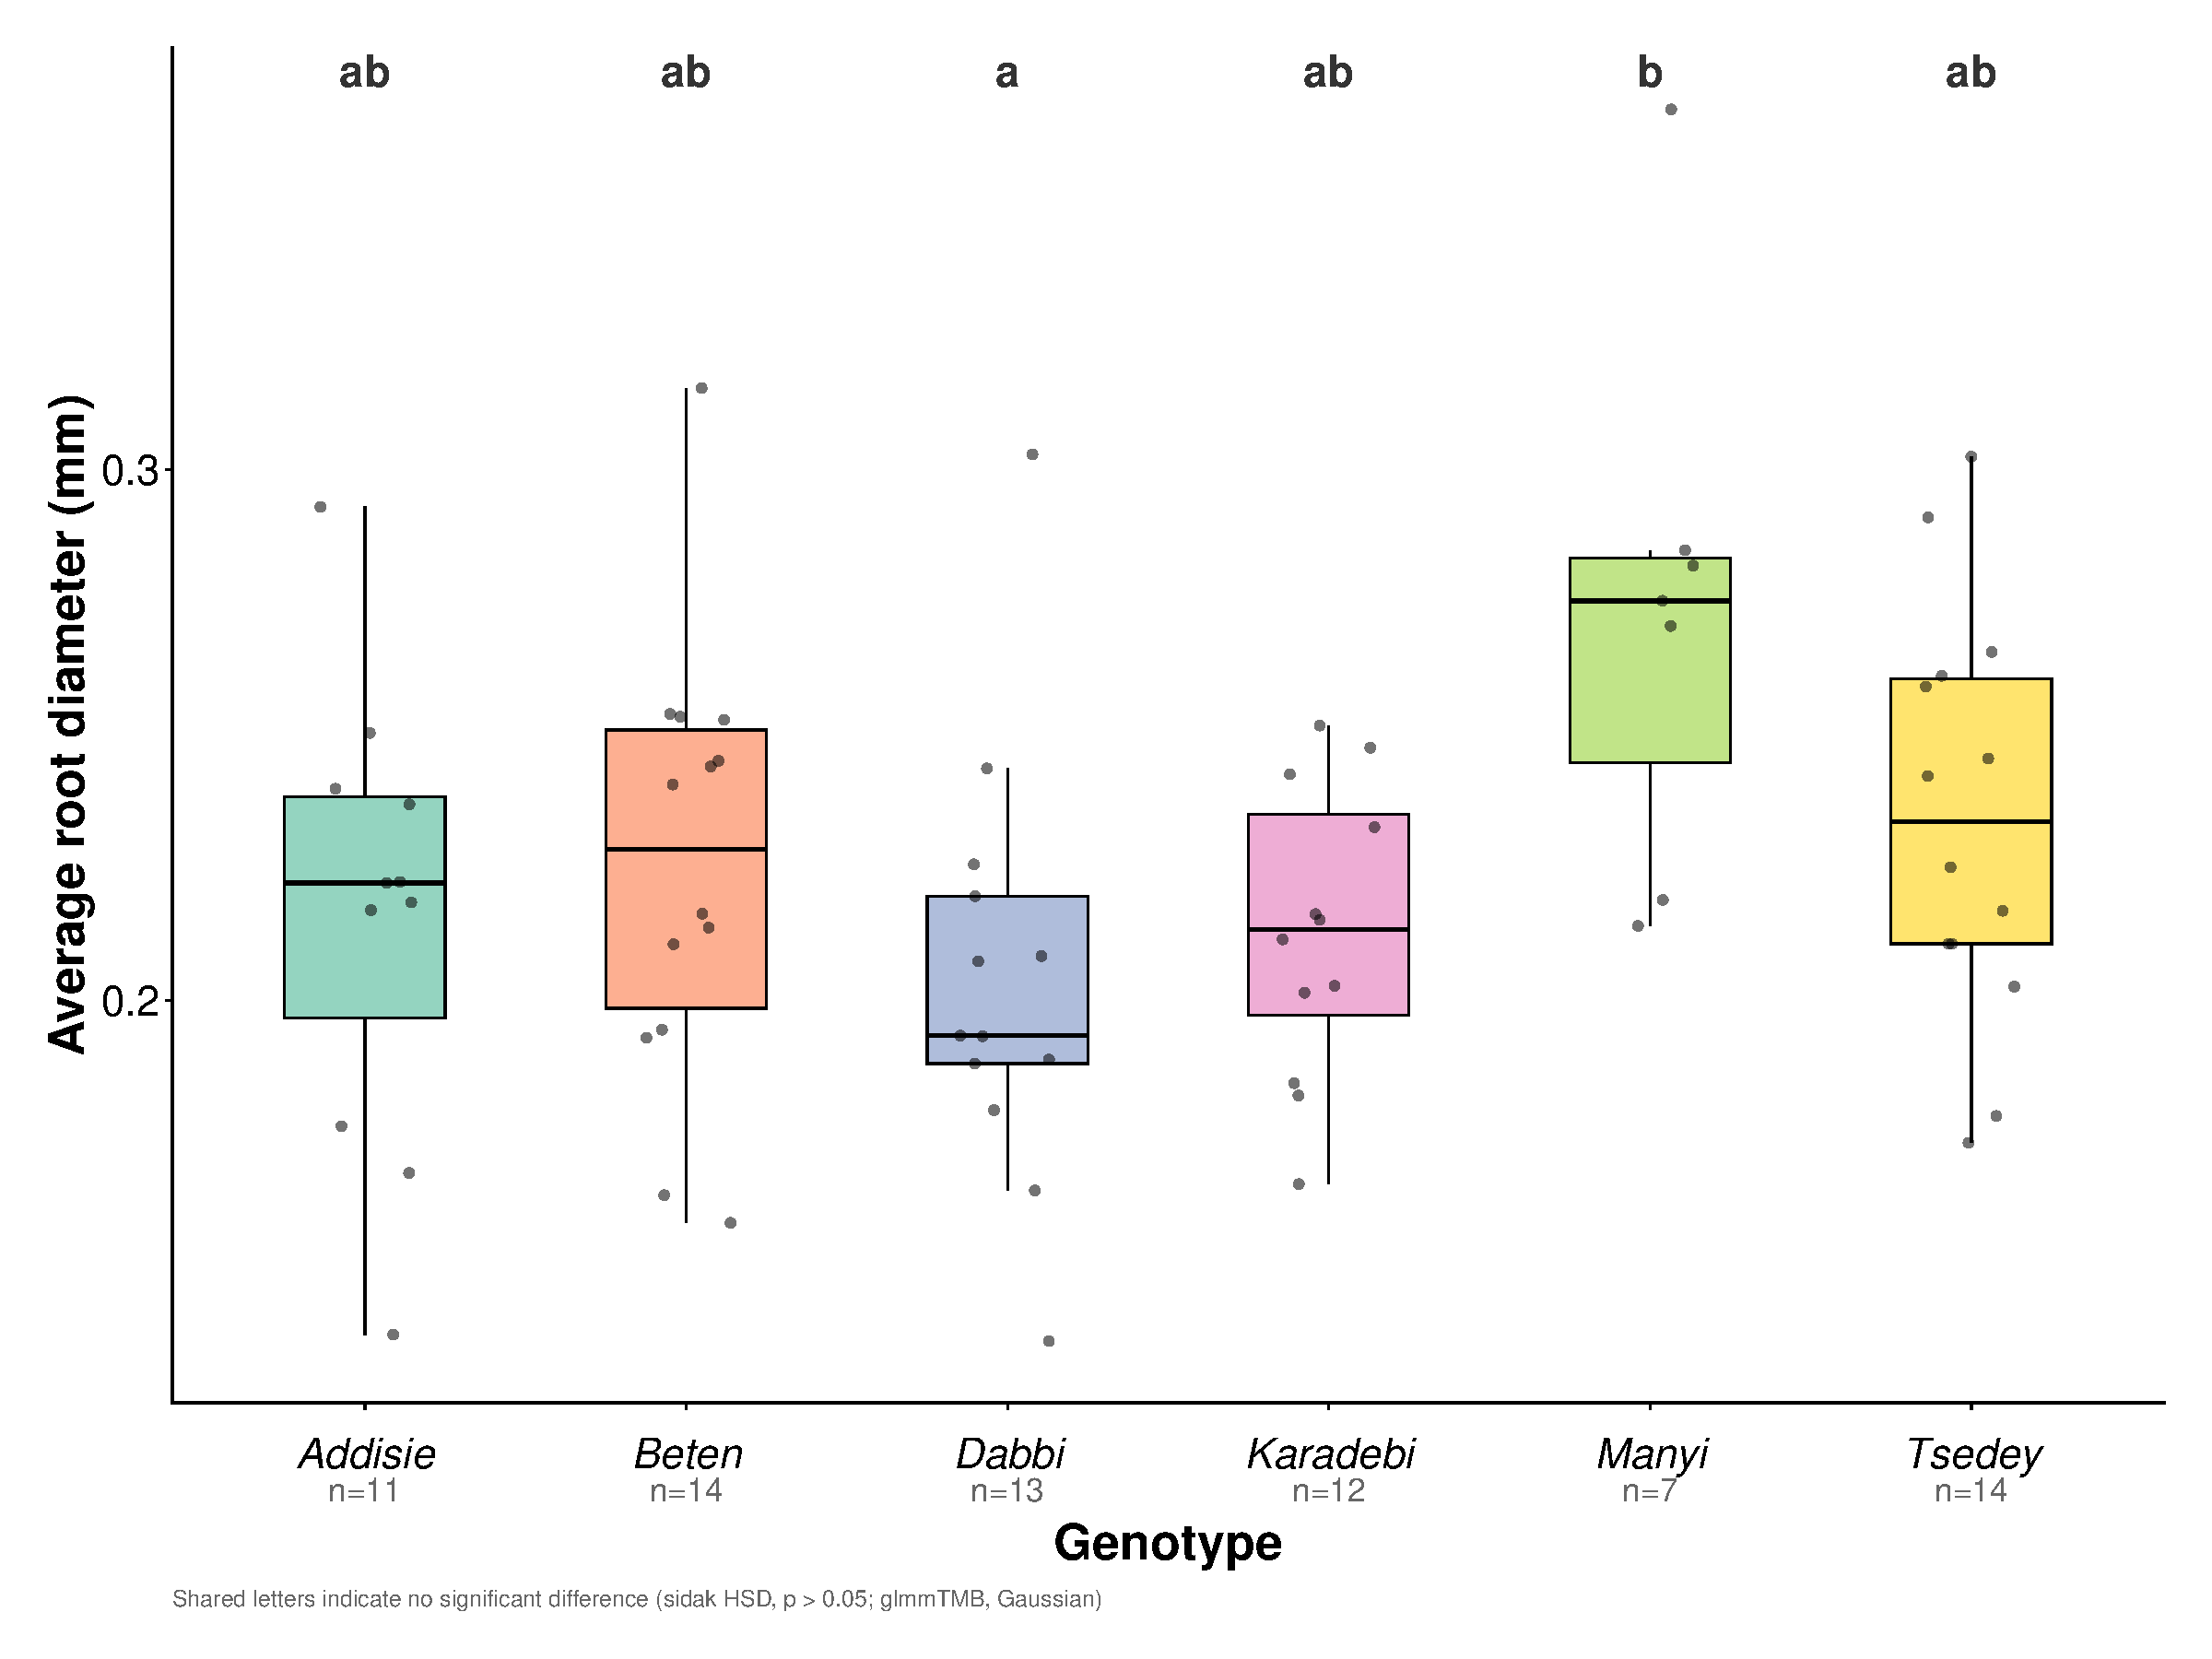
\includegraphics[keepaspectratio]{rsa_day1617_agar_files/figure-pdf/unnamed-chunk-4-6.pdf}}

\subsubsection{Convex Area}\label{convex-area}

\begin{Shaded}
\begin{Highlighting}[]
\CommentTok{\# ── 1. Inspect the trait ──────────────────────────────────────}
\FunctionTok{summary}\NormalTok{(df}\SpecialCharTok{$}\NormalTok{Convex.Area.mm2)}
\end{Highlighting}
\end{Shaded}

\begin{verbatim}
   Min. 1st Qu.  Median    Mean 3rd Qu.    Max. 
  39.09  176.93  370.90  511.17  670.98 2115.25 
\end{verbatim}

\begin{Shaded}
\begin{Highlighting}[]
\FunctionTok{hist}\NormalTok{(df}\SpecialCharTok{$}\NormalTok{Convex.Area.mm2, }\AttributeTok{breaks =} \DecValTok{15}\NormalTok{, }\AttributeTok{main =} \StringTok{"Convex Area distribution"}\NormalTok{)}
\end{Highlighting}
\end{Shaded}

\pandocbounded{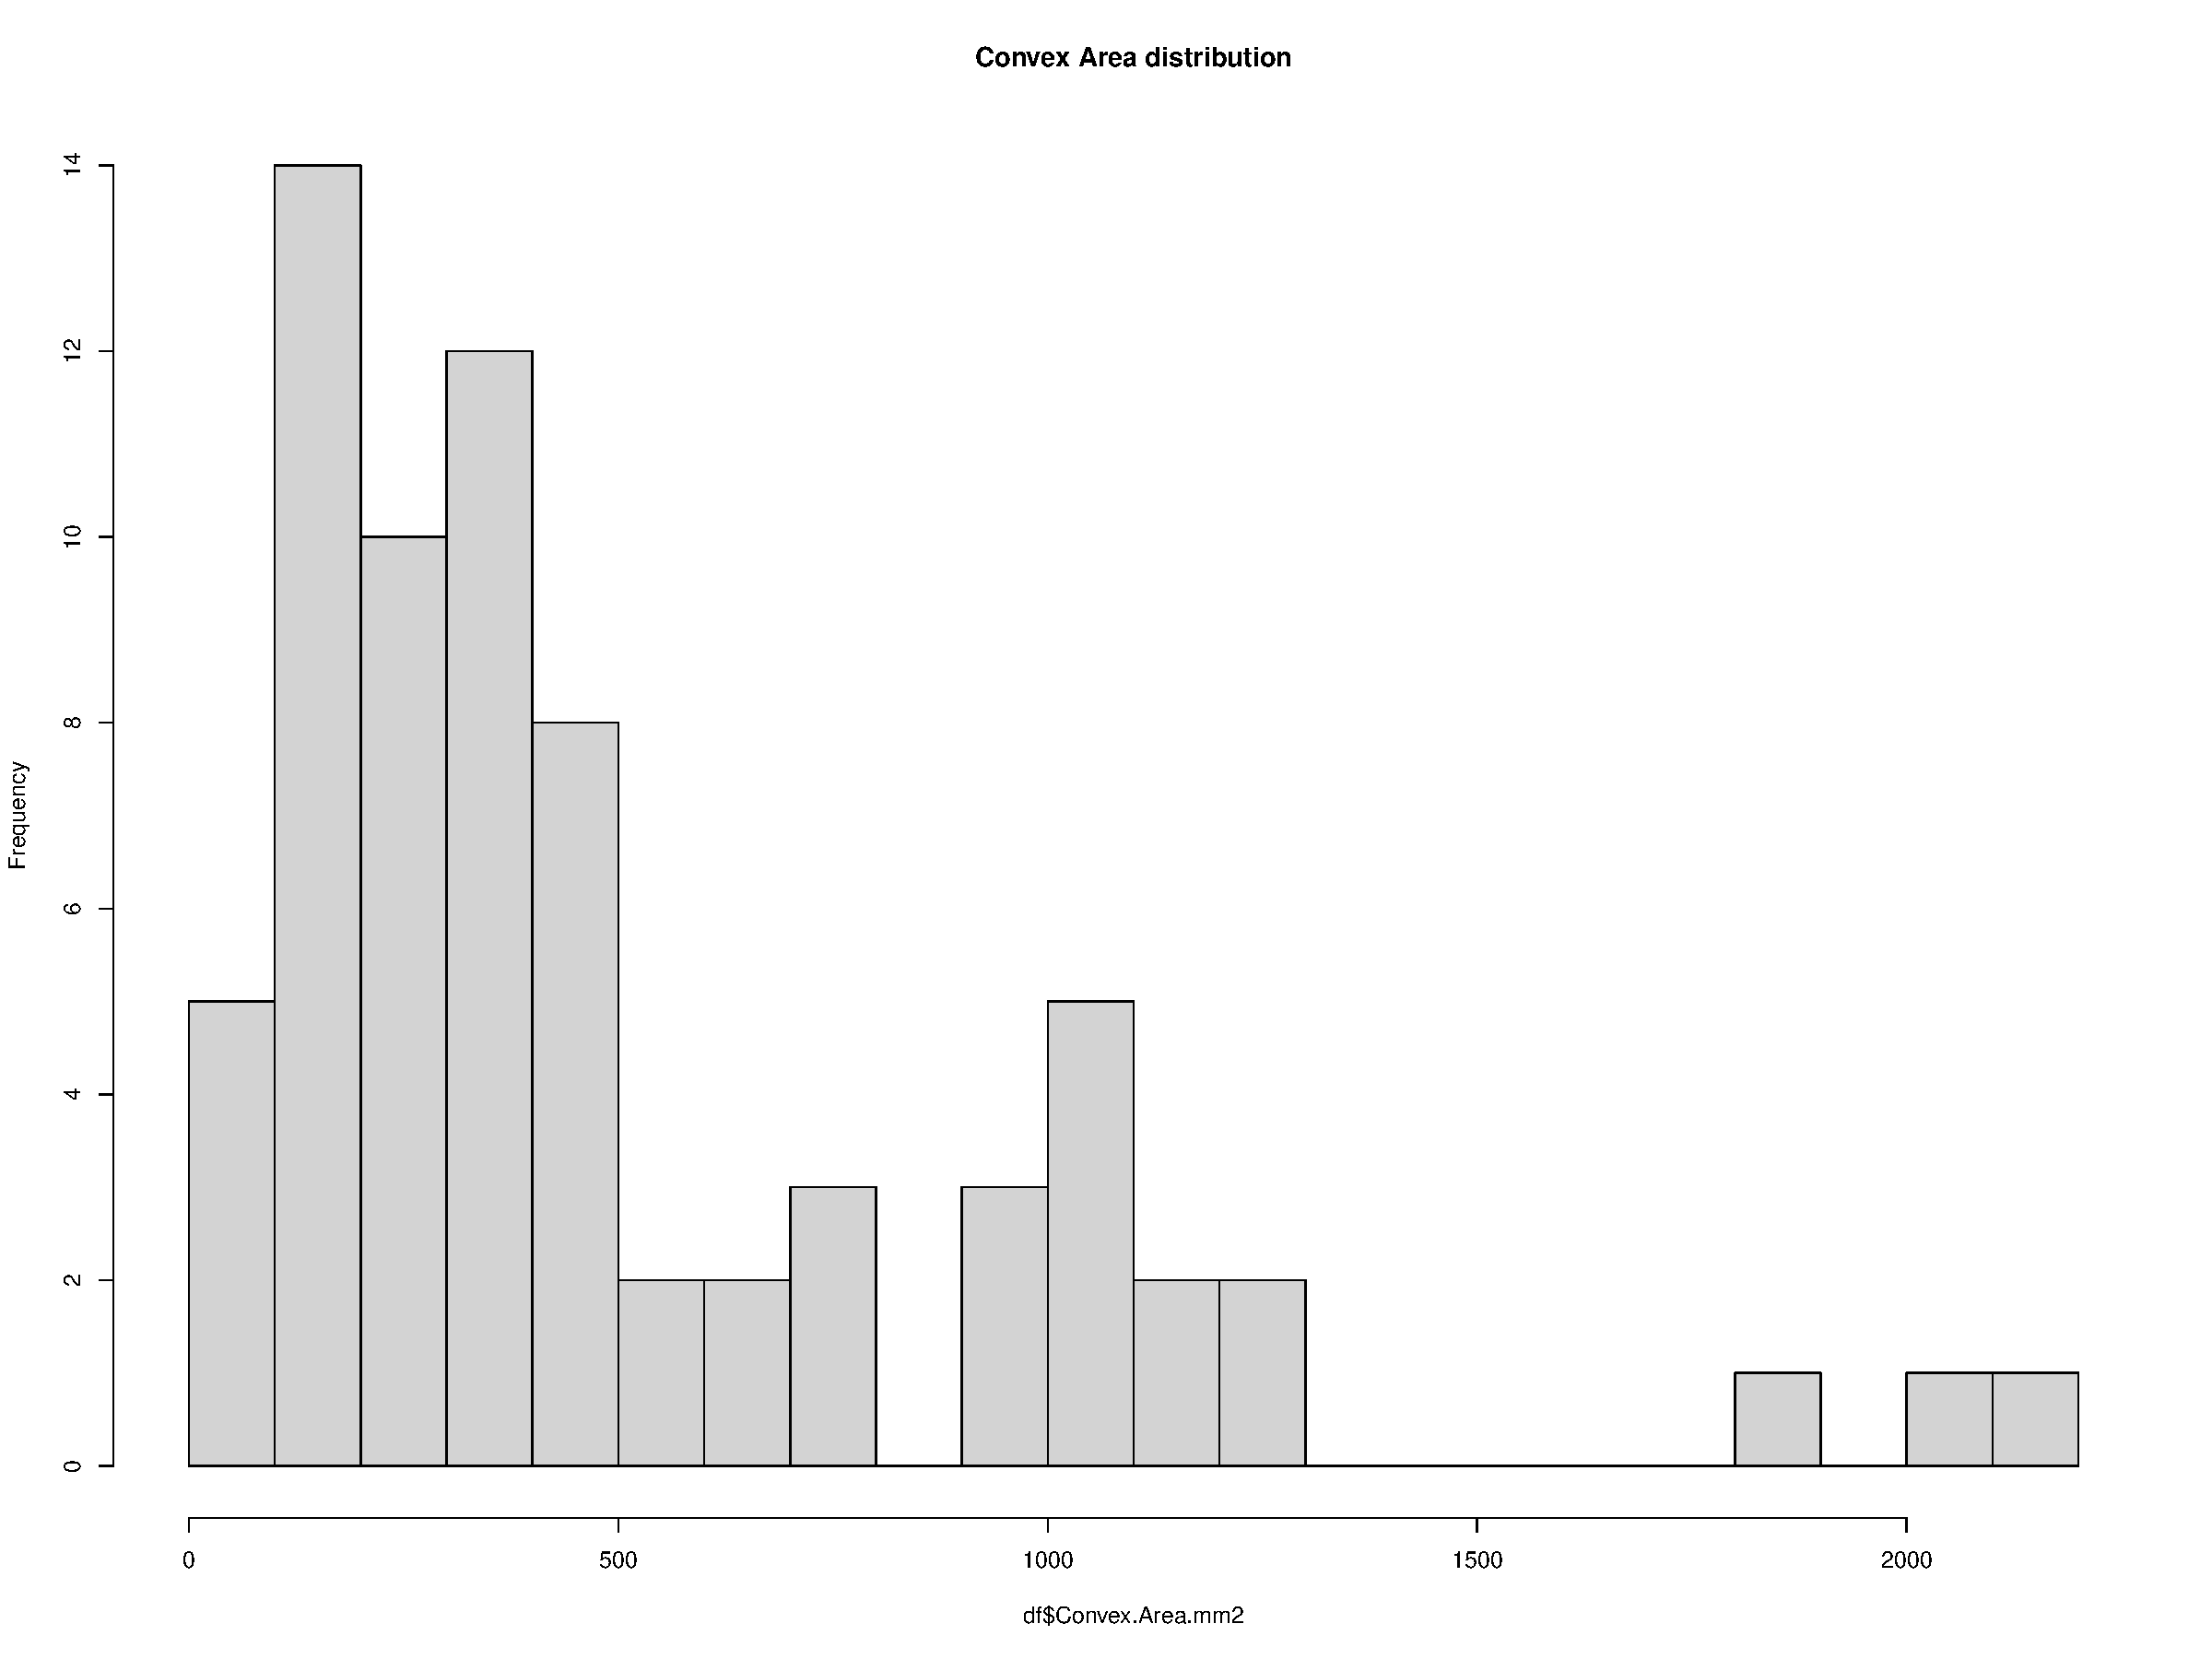
\includegraphics[keepaspectratio]{rsa_day1617_agar_files/figure-pdf/unnamed-chunk-5-1.pdf}}

\begin{Shaded}
\begin{Highlighting}[]
\CommentTok{\# ── 1. Fit full nested model ──────────────────────────────────}
\NormalTok{convex\_full }\OtherTok{\textless{}{-}} \FunctionTok{glmmTMB}\NormalTok{(}
\NormalTok{  (Convex.Area.mm2) }\SpecialCharTok{\textasciitilde{}}\NormalTok{ Genotype }\SpecialCharTok{+}\NormalTok{ (}\DecValTok{1} \SpecialCharTok{|}\NormalTok{ Batch}\SpecialCharTok{/}\NormalTok{Plate}\SpecialCharTok{/}\NormalTok{Seed),}
  \AttributeTok{data =}\NormalTok{ df, }\AttributeTok{family =} \FunctionTok{gaussian}\NormalTok{()}
\NormalTok{)}
\end{Highlighting}
\end{Shaded}

\begin{verbatim}
Warning in finalizeTMB(TMBStruc, obj, fit, h, data.tmb.old): Model convergence
problem; non-positive-definite Hessian matrix. See vignette('troubleshooting')
\end{verbatim}

\begin{Shaded}
\begin{Highlighting}[]
\FunctionTok{VarCorr}\NormalTok{(convex\_full)}
\end{Highlighting}
\end{Shaded}

\begin{verbatim}

Conditional model:
 Groups           Name        Std.Dev.  
 Seed:Plate:Batch (Intercept) 1.2363e-95
 Plate:Batch      (Intercept) 5.0799e-01
 Batch            (Intercept) 2.0434e+02
 Residual                     3.7626e+02
\end{verbatim}

\begin{Shaded}
\begin{Highlighting}[]
\FunctionTok{check\_singularity}\NormalTok{(convex\_full) }
\end{Highlighting}
\end{Shaded}

\begin{verbatim}
[1] TRUE
\end{verbatim}

\begin{Shaded}
\begin{Highlighting}[]
\CommentTok{\# get error:   Model convergence problem; non{-}positive{-}definite Hessian matrix. See vignette(\textquotesingle{}troubleshooting\textquotesingle{})}
\CommentTok{\# will simplify model as std. dev. of seed:plate:batch is incredibly small (1.2363e{-}95)}

\CommentTok{\# ── 3. Simplified model (only if full model fails) ────────────}
\NormalTok{convex\_tmb }\OtherTok{\textless{}{-}} \FunctionTok{glmmTMB}\NormalTok{(}
\NormalTok{  (Convex.Area.mm2) }\SpecialCharTok{\textasciitilde{}}\NormalTok{ Genotype }\SpecialCharTok{+}\NormalTok{ (}\DecValTok{1} \SpecialCharTok{|}\NormalTok{ Batch}\SpecialCharTok{/}\NormalTok{Plate),}
  \AttributeTok{data =}\NormalTok{ df, }\AttributeTok{family =} \FunctionTok{gaussian}\NormalTok{()}
\NormalTok{)}

\FunctionTok{VarCorr}\NormalTok{(convex\_tmb)}
\end{Highlighting}
\end{Shaded}

\begin{verbatim}

Conditional model:
 Groups      Name        Std.Dev.  
 Plate:Batch (Intercept) 1.8678e-14
 Batch       (Intercept) 2.0363e+02
 Residual                3.7632e+02
\end{verbatim}

\begin{Shaded}
\begin{Highlighting}[]
\FunctionTok{summary}\NormalTok{(convex\_tmb)}
\end{Highlighting}
\end{Shaded}

\begin{verbatim}
 Family: gaussian  ( identity )
Formula:          (Convex.Area.mm2) ~ Genotype + (1 | Batch/Plate)
Data: df

      AIC       BIC    logLik -2*log(L)  df.resid 
   1068.9    1089.2    -525.4    1050.9        62 

Random effects:

Conditional model:
 Groups      Name        Variance  Std.Dev. 
 Plate:Batch (Intercept) 3.489e-28 1.868e-14
 Batch       (Intercept) 4.147e+04 2.036e+02
 Residual                1.416e+05 3.763e+02
Number of obs: 71, groups:  Plate:Batch, 18; Batch, 4

Dispersion estimate for gaussian family (sigma^2): 1.42e+05 

Conditional model:
                 Estimate Std. Error z value Pr(>|z|)
(Intercept)         747.0        NaN     NaN      NaN
GenotypeBeten      -124.0        NaN     NaN      NaN
GenotypeDabbi      -336.4        NaN     NaN      NaN
GenotypeKaradebi   -182.7        NaN     NaN      NaN
GenotypeManyi      -376.0        NaN     NaN      NaN
GenotypeTsedey     -409.1        NaN     NaN      NaN
\end{verbatim}

\begin{Shaded}
\begin{Highlighting}[]
\FunctionTok{check\_singularity}\NormalTok{(convex\_tmb) }
\end{Highlighting}
\end{Shaded}

\begin{verbatim}
[1] TRUE
\end{verbatim}

\begin{Shaded}
\begin{Highlighting}[]
\CommentTok{\# plate:batch has very small effect and get NaNs inc conditional model so will drop plate effect}

\CommentTok{\# Plate interaction is incredibly small so will drop }
\CommentTok{\# ── 3. Simplified model (only if simplified model fails) ────────────}
\NormalTok{convex\_tmb }\OtherTok{\textless{}{-}} \FunctionTok{glmmTMB}\NormalTok{(}
\NormalTok{  (Convex.Area.mm2) }\SpecialCharTok{\textasciitilde{}}\NormalTok{ Genotype }\SpecialCharTok{+}\NormalTok{ (}\DecValTok{1} \SpecialCharTok{|}\NormalTok{ Batch),}
  \AttributeTok{data =}\NormalTok{ df, }\AttributeTok{family =} \FunctionTok{gaussian}\NormalTok{()}
\NormalTok{)}

\FunctionTok{VarCorr}\NormalTok{(convex\_tmb)}
\end{Highlighting}
\end{Shaded}

\begin{verbatim}

Conditional model:
 Groups   Name        Std.Dev.
 Batch    (Intercept) 204.23  
 Residual             376.27  
\end{verbatim}

\begin{Shaded}
\begin{Highlighting}[]
\FunctionTok{check\_singularity}\NormalTok{(convex\_tmb) }
\end{Highlighting}
\end{Shaded}

\begin{verbatim}
[1] FALSE
\end{verbatim}

\begin{Shaded}
\begin{Highlighting}[]
\CommentTok{\# ── 4. Assumption checks (on whichever model passed) ─────────}
\NormalTok{sim\_res }\OtherTok{\textless{}{-}} \FunctionTok{simulateResiduals}\NormalTok{(convex\_tmb, }\AttributeTok{n =} \DecValTok{1000}\NormalTok{)}
\FunctionTok{plot}\NormalTok{(sim\_res)                               }\CommentTok{\# QQ + residuals vs fitted}
\end{Highlighting}
\end{Shaded}

\pandocbounded{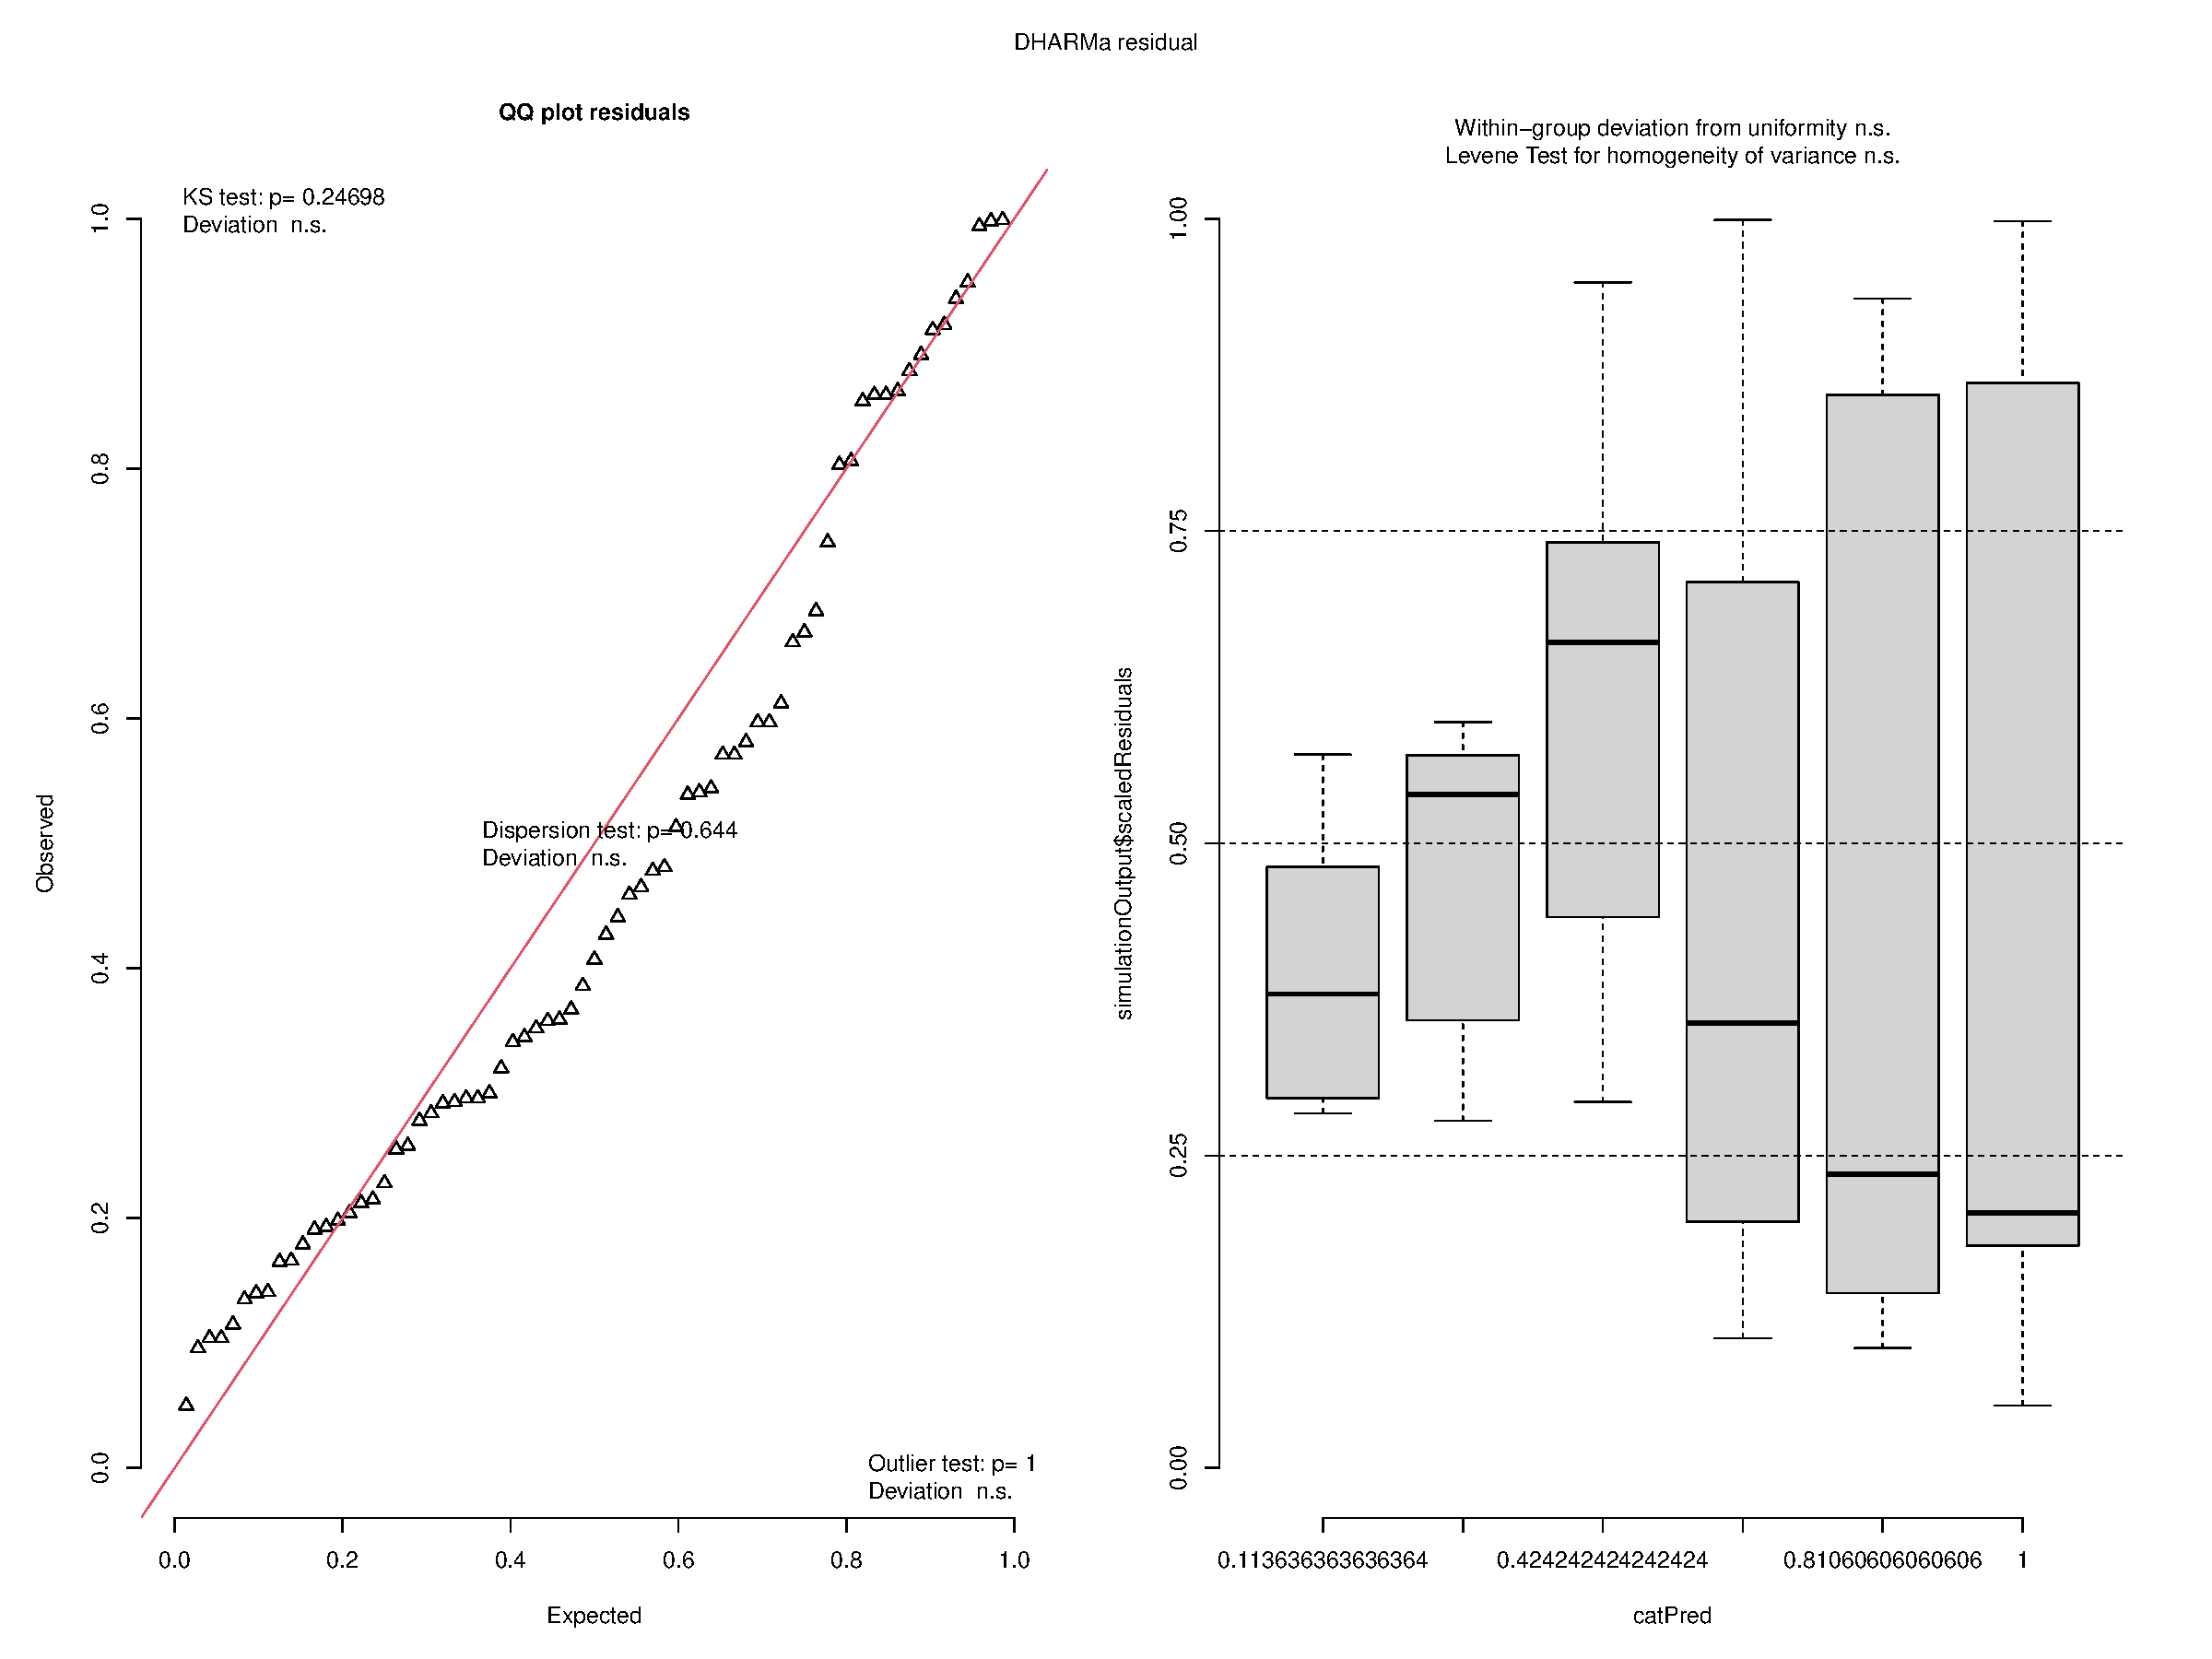
\includegraphics[keepaspectratio]{rsa_day1617_agar_files/figure-pdf/unnamed-chunk-5-2.pdf}}

\begin{Shaded}
\begin{Highlighting}[]
\FunctionTok{testUniformity}\NormalTok{(sim\_res)                     }\CommentTok{\# p \textgreater{} 0.05 = distribution correct}
\end{Highlighting}
\end{Shaded}

\pandocbounded{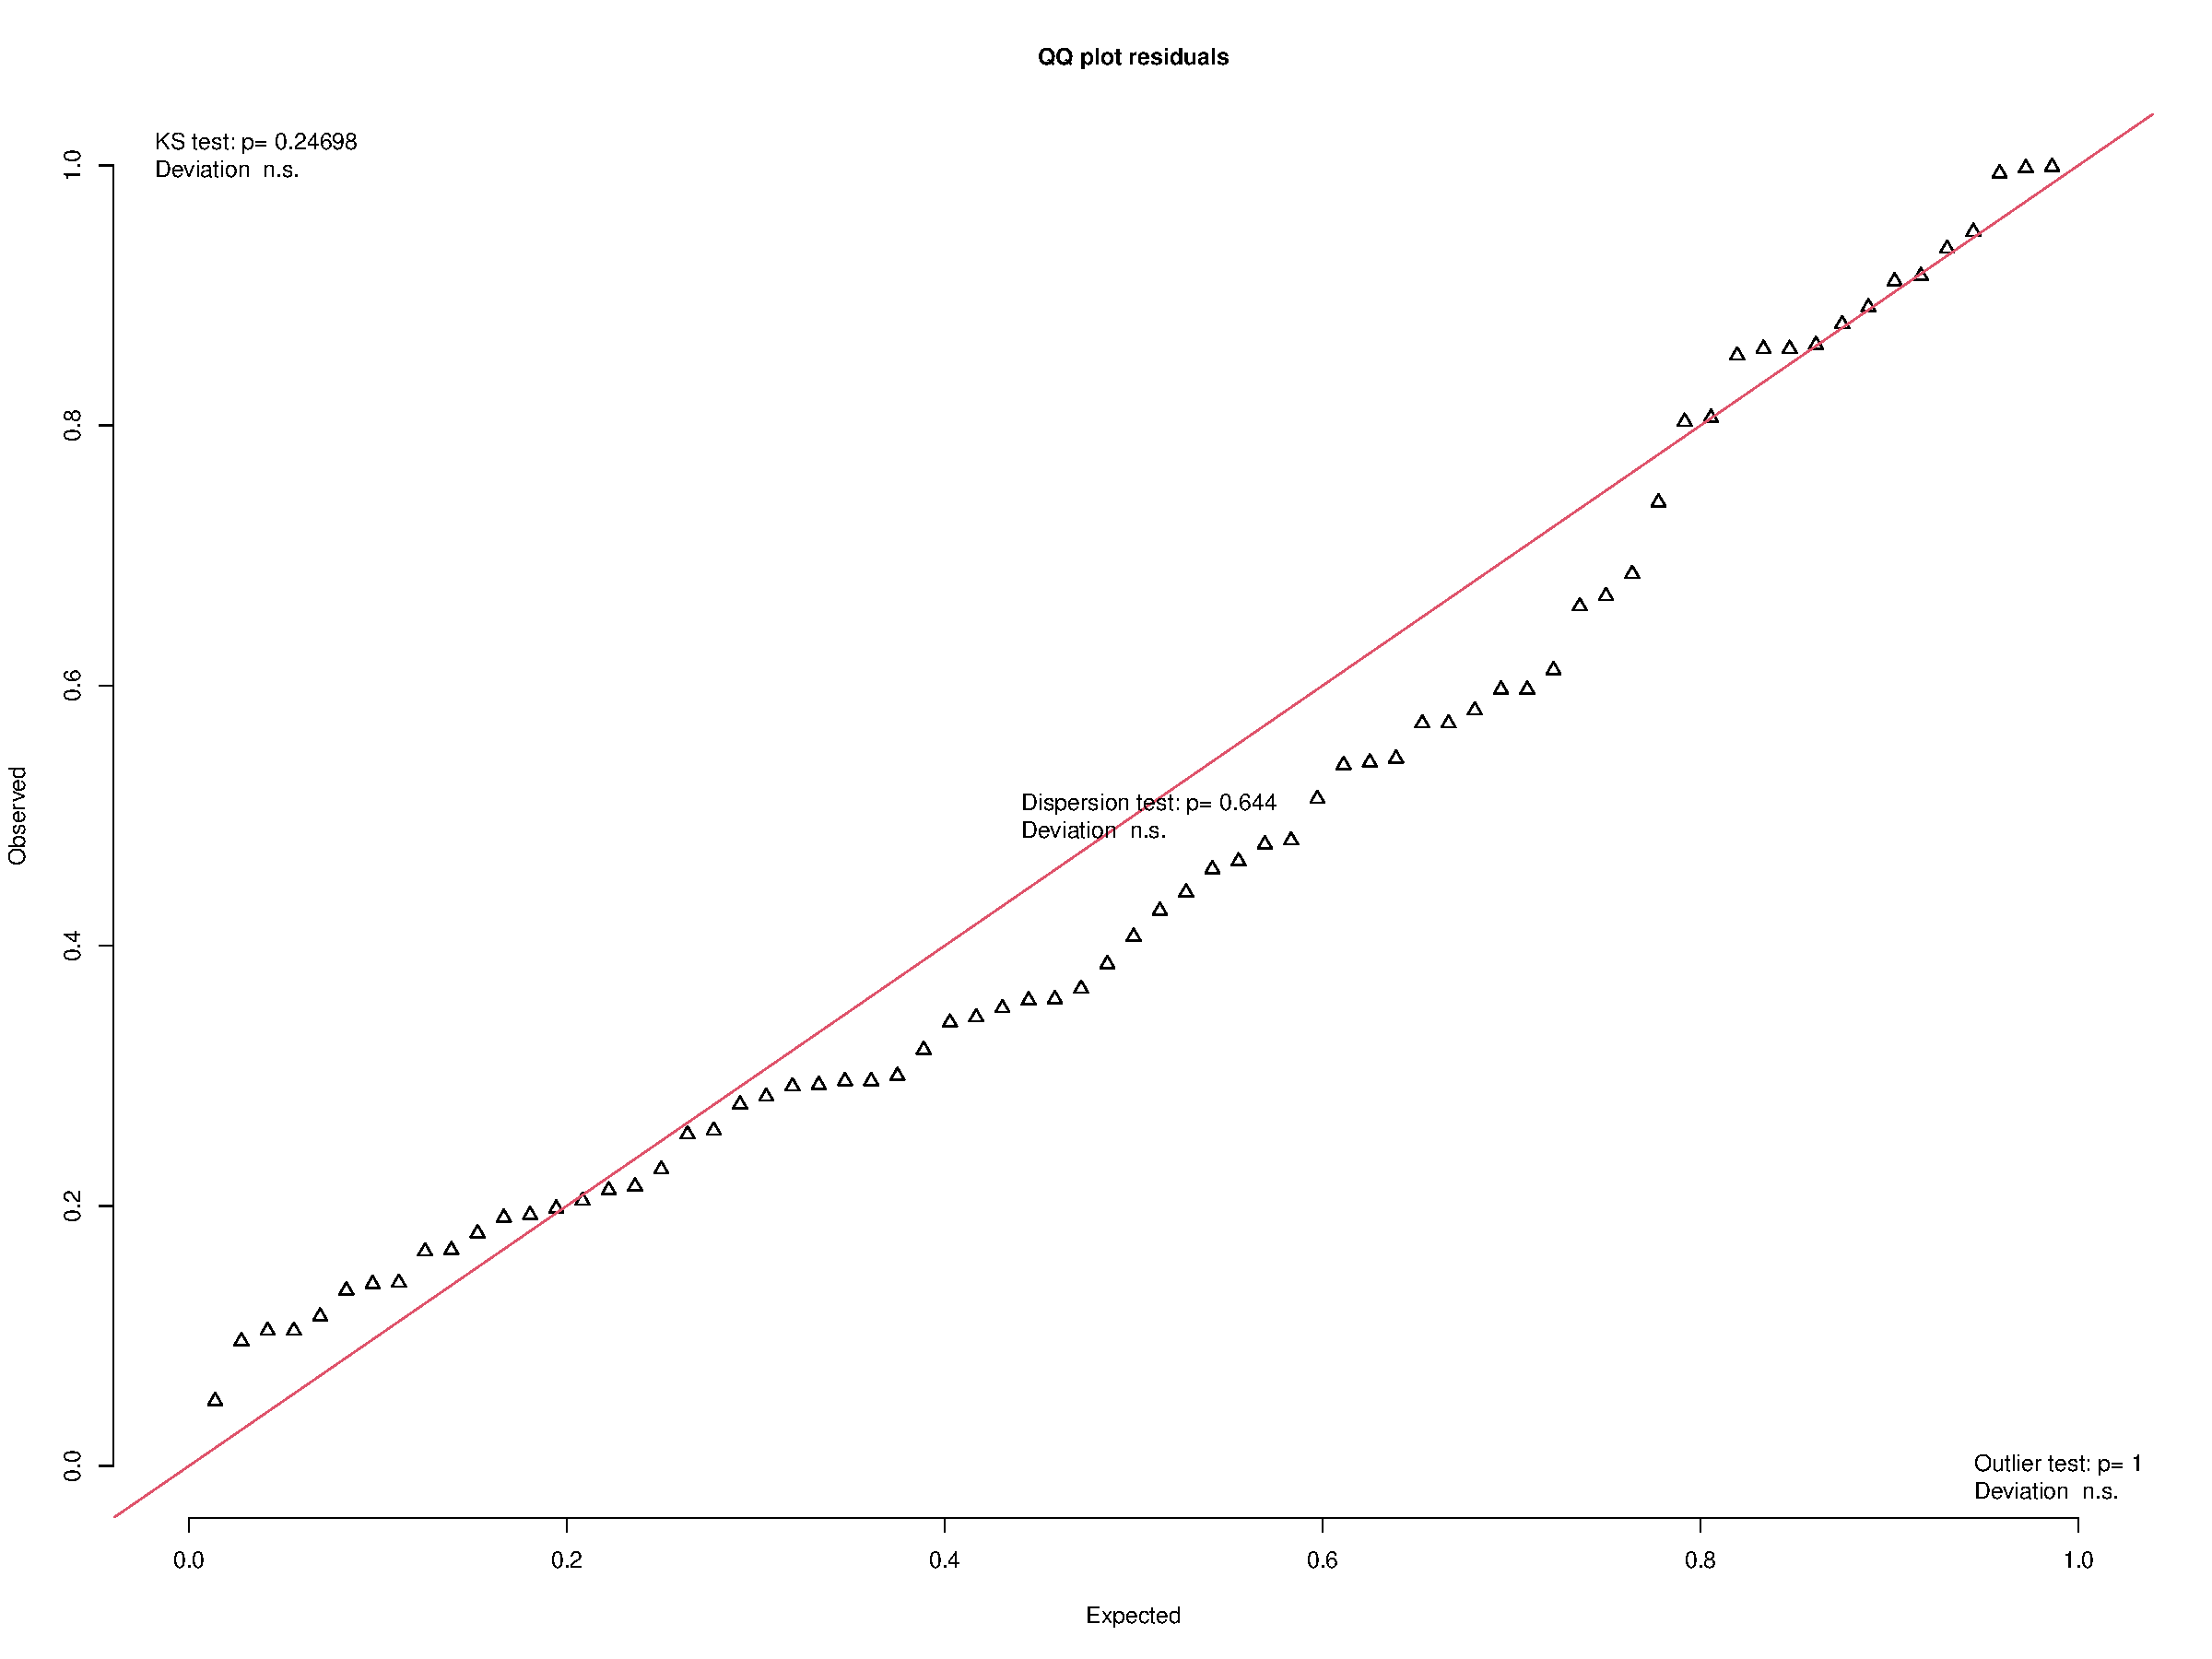
\includegraphics[keepaspectratio]{rsa_day1617_agar_files/figure-pdf/unnamed-chunk-5-3.pdf}}

\begin{verbatim}

    Asymptotic one-sample Kolmogorov-Smirnov test

data:  simulationOutput$scaledResiduals
D = 0.12131, p-value = 0.247
alternative hypothesis: two-sided
\end{verbatim}

\begin{Shaded}
\begin{Highlighting}[]
\FunctionTok{testDispersion}\NormalTok{(sim\_res)                     }\CommentTok{\# ratio ≈ 1.0}
\end{Highlighting}
\end{Shaded}

\pandocbounded{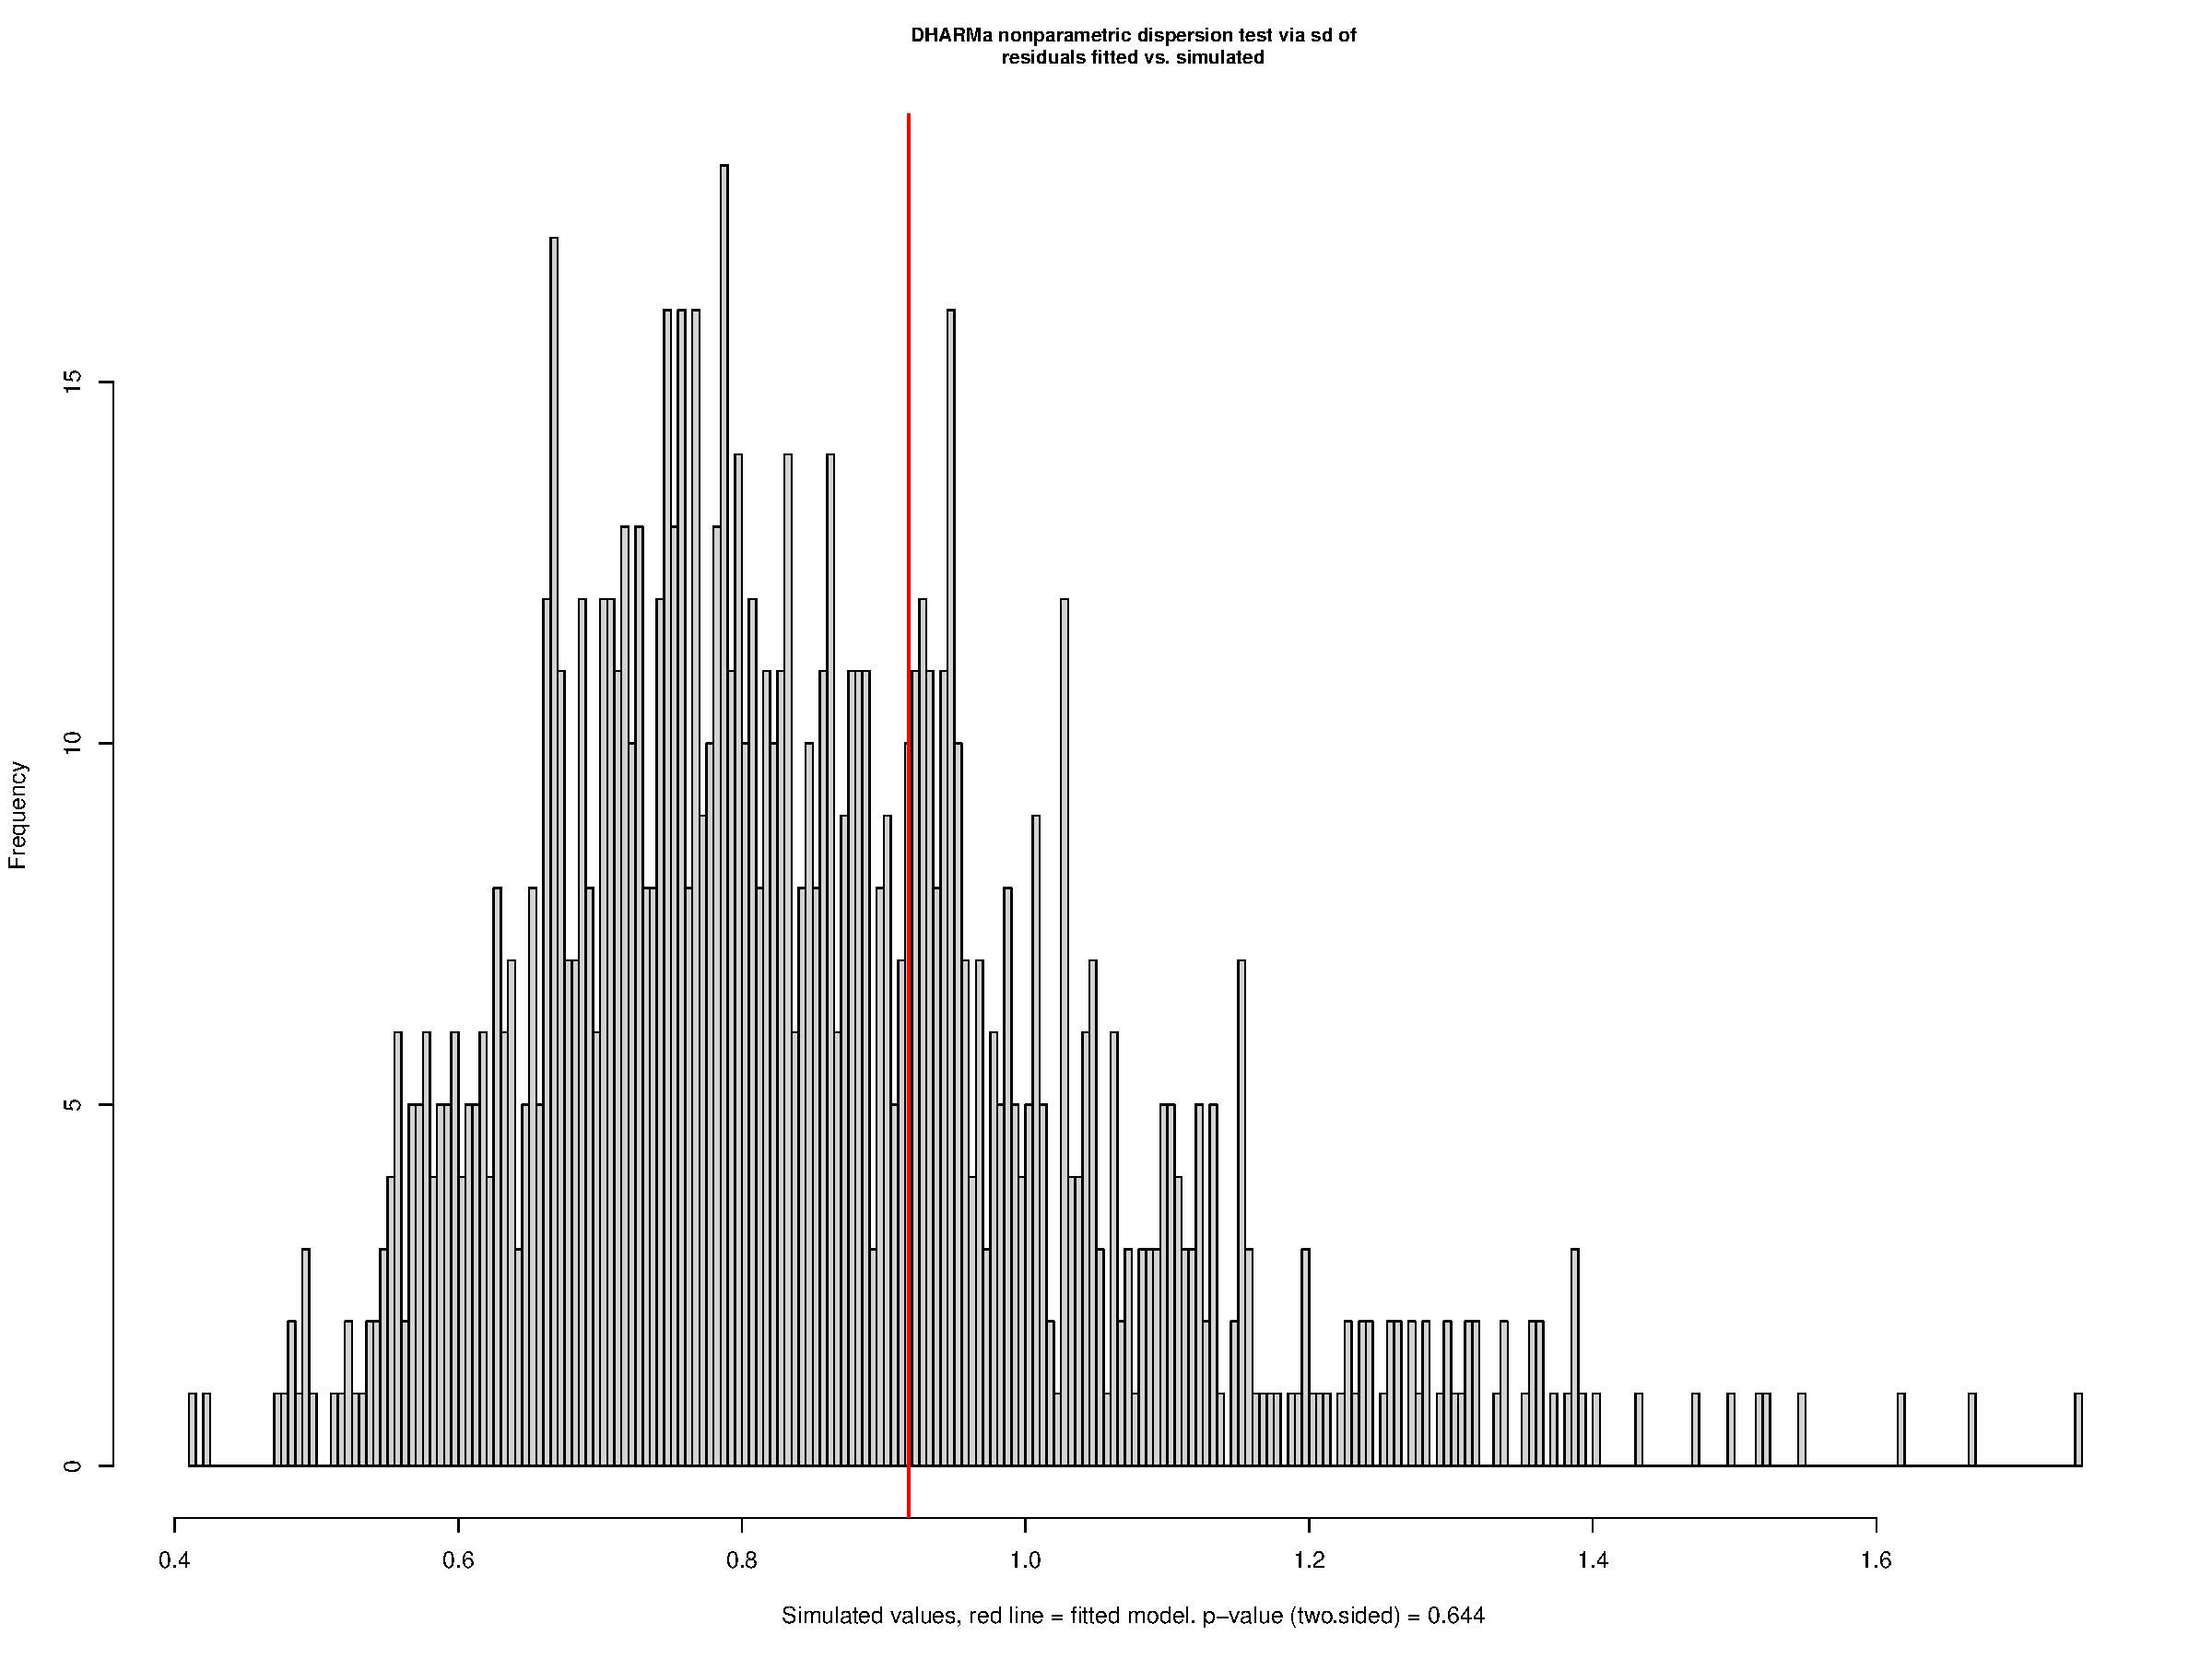
\includegraphics[keepaspectratio]{rsa_day1617_agar_files/figure-pdf/unnamed-chunk-5-4.pdf}}

\begin{verbatim}

    DHARMa nonparametric dispersion test via sd of residuals fitted vs.
    simulated

data:  simulationOutput
dispersion = 1.0821, p-value = 0.644
alternative hypothesis: two.sided
\end{verbatim}

\begin{Shaded}
\begin{Highlighting}[]
\FunctionTok{plotResiduals}\NormalTok{(sim\_res, }\AttributeTok{form =}\NormalTok{ df}\SpecialCharTok{$}\NormalTok{Genotype)  }\CommentTok{\# no patterns per genotype}
\end{Highlighting}
\end{Shaded}

\pandocbounded{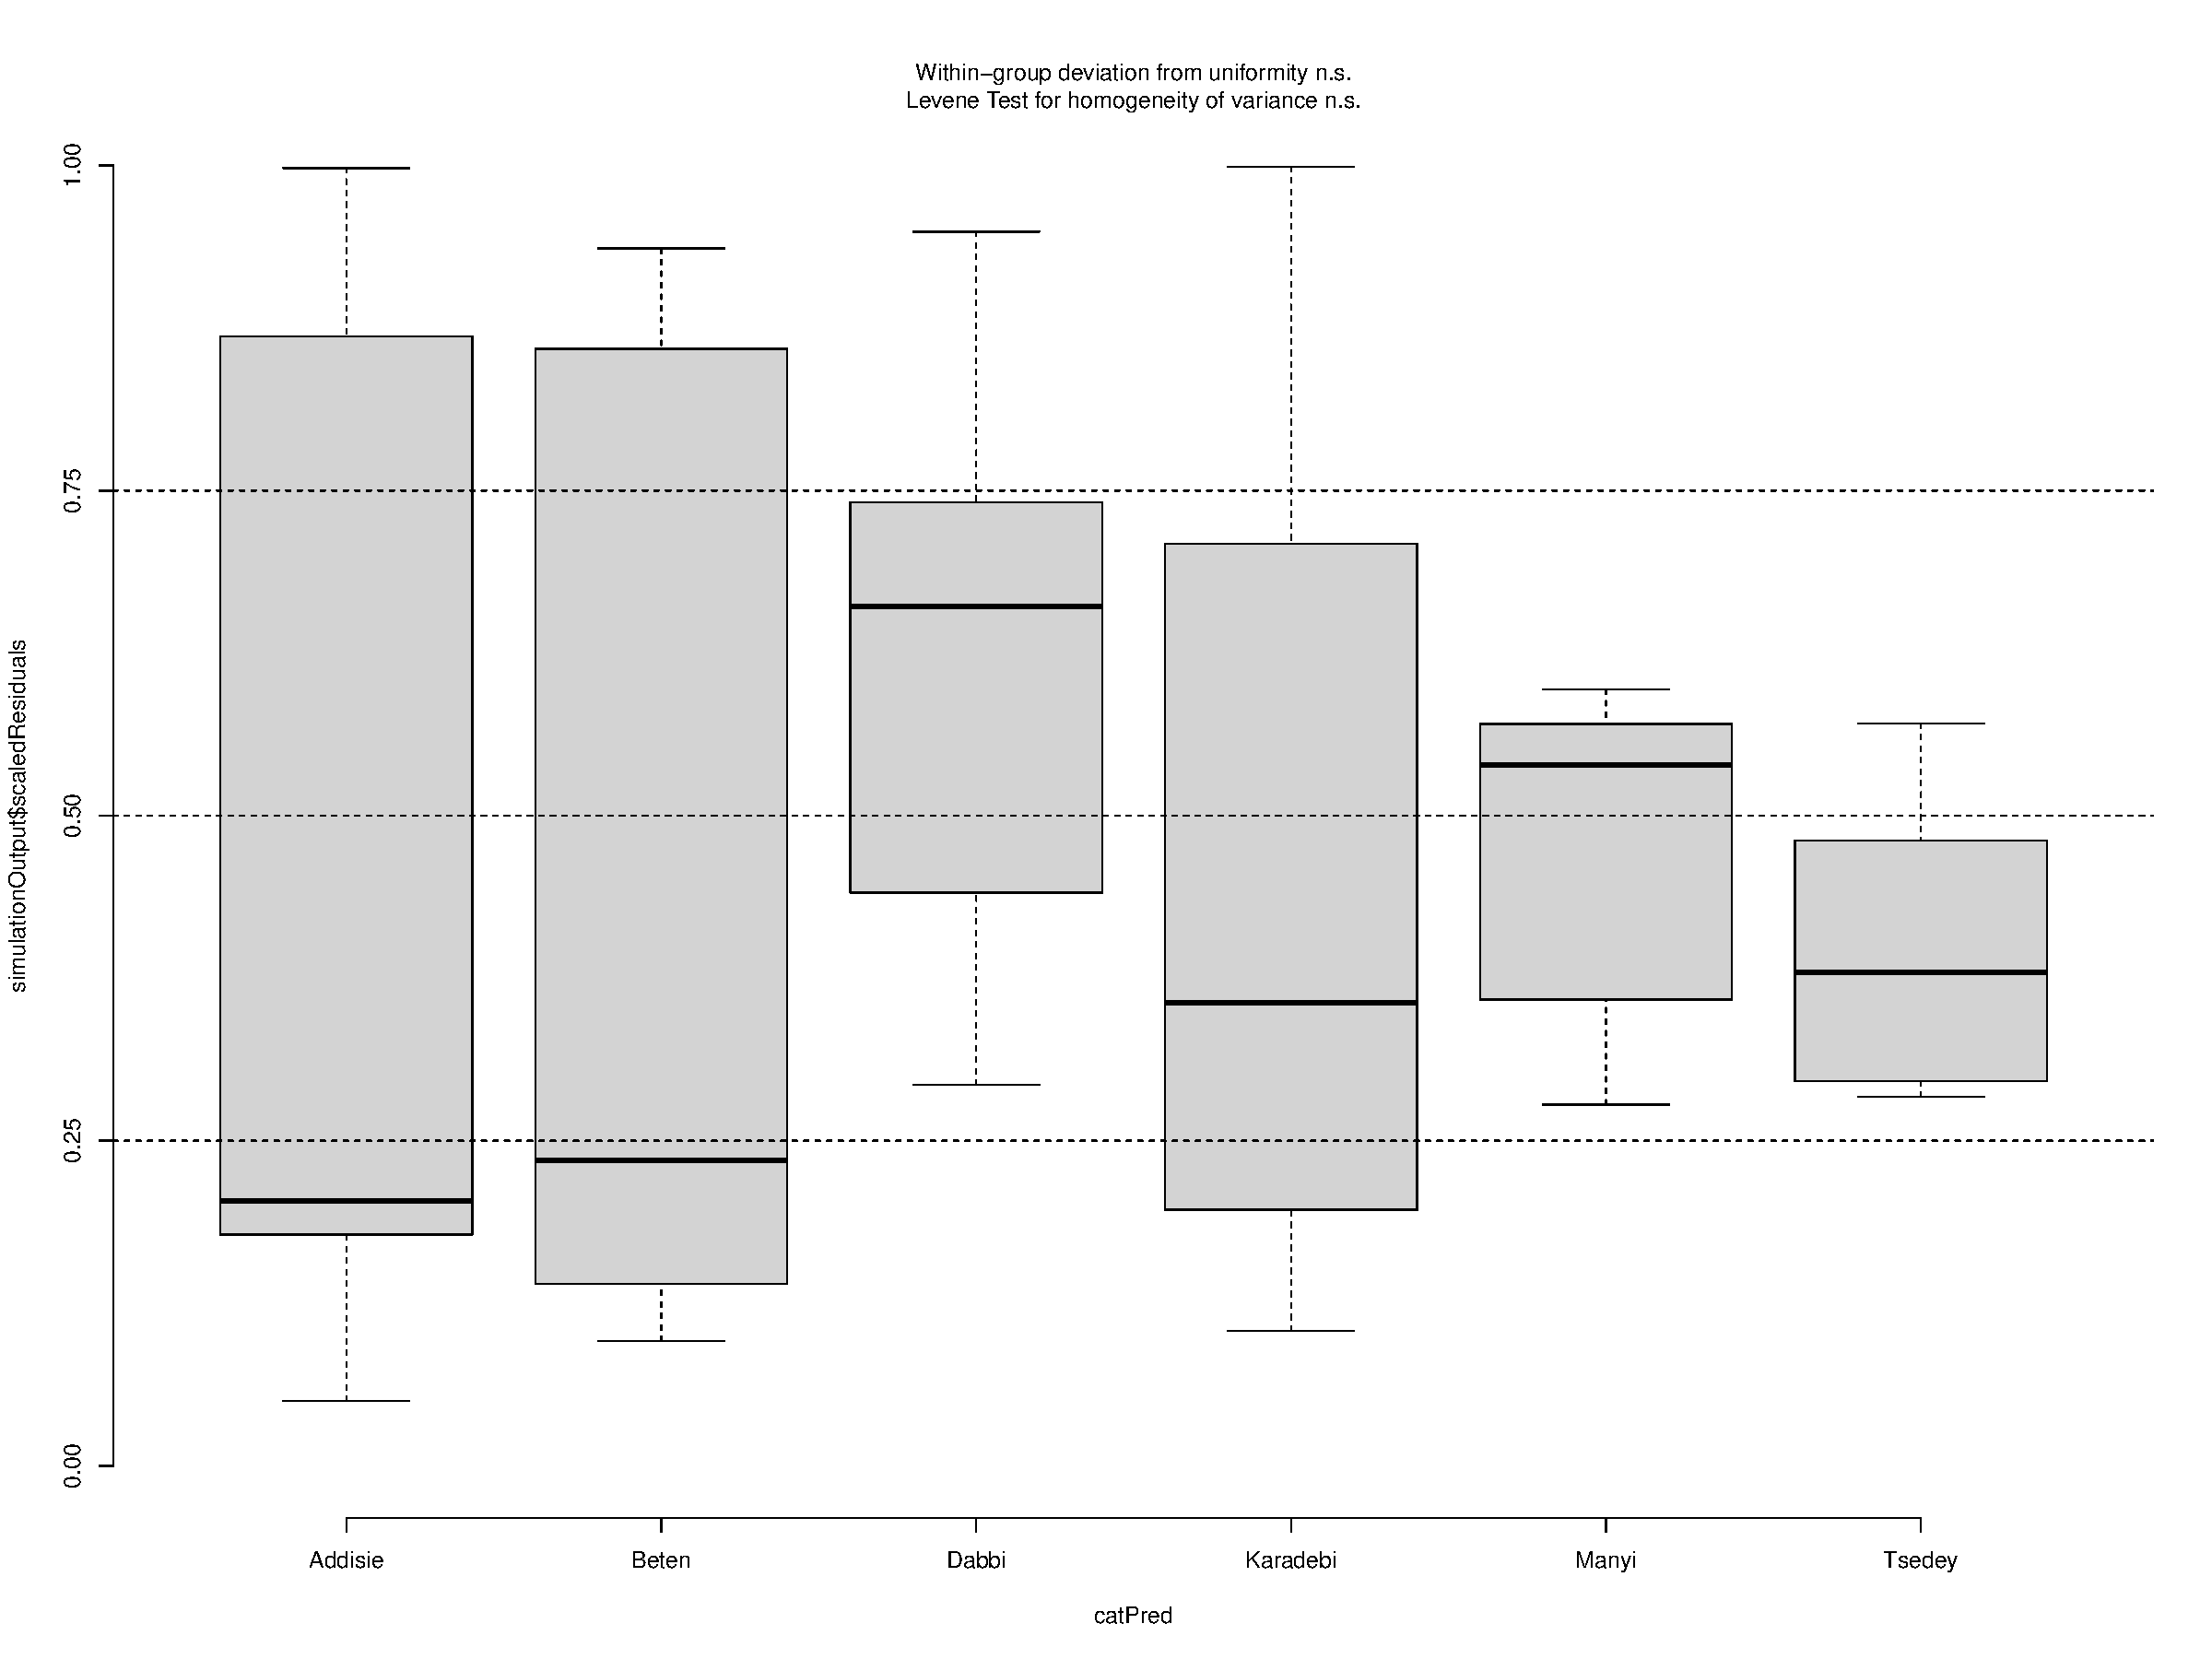
\includegraphics[keepaspectratio]{rsa_day1617_agar_files/figure-pdf/unnamed-chunk-5-5.pdf}}

\begin{Shaded}
\begin{Highlighting}[]
\CommentTok{\# residuals show that there is some snaking so will try log transforming to see if fit is better }

\NormalTok{convex\_tmb }\OtherTok{\textless{}{-}} \FunctionTok{glmmTMB}\NormalTok{( }\FunctionTok{log}\NormalTok{(Convex.Area.mm2) }\SpecialCharTok{\textasciitilde{}}\NormalTok{ Genotype }\SpecialCharTok{+}\NormalTok{ (}\DecValTok{1} \SpecialCharTok{|}\NormalTok{ Batch), }\AttributeTok{data =}\NormalTok{ df, }\AttributeTok{family =} \FunctionTok{gaussian}\NormalTok{() ) }
\NormalTok{sim\_res }\OtherTok{\textless{}{-}} \FunctionTok{simulateResiduals}\NormalTok{(convex\_tmb, }\AttributeTok{n =} \DecValTok{1000}\NormalTok{)}
\FunctionTok{plot}\NormalTok{(sim\_res)                               }\CommentTok{\# QQ + residuals vs fitted}
\end{Highlighting}
\end{Shaded}

\pandocbounded{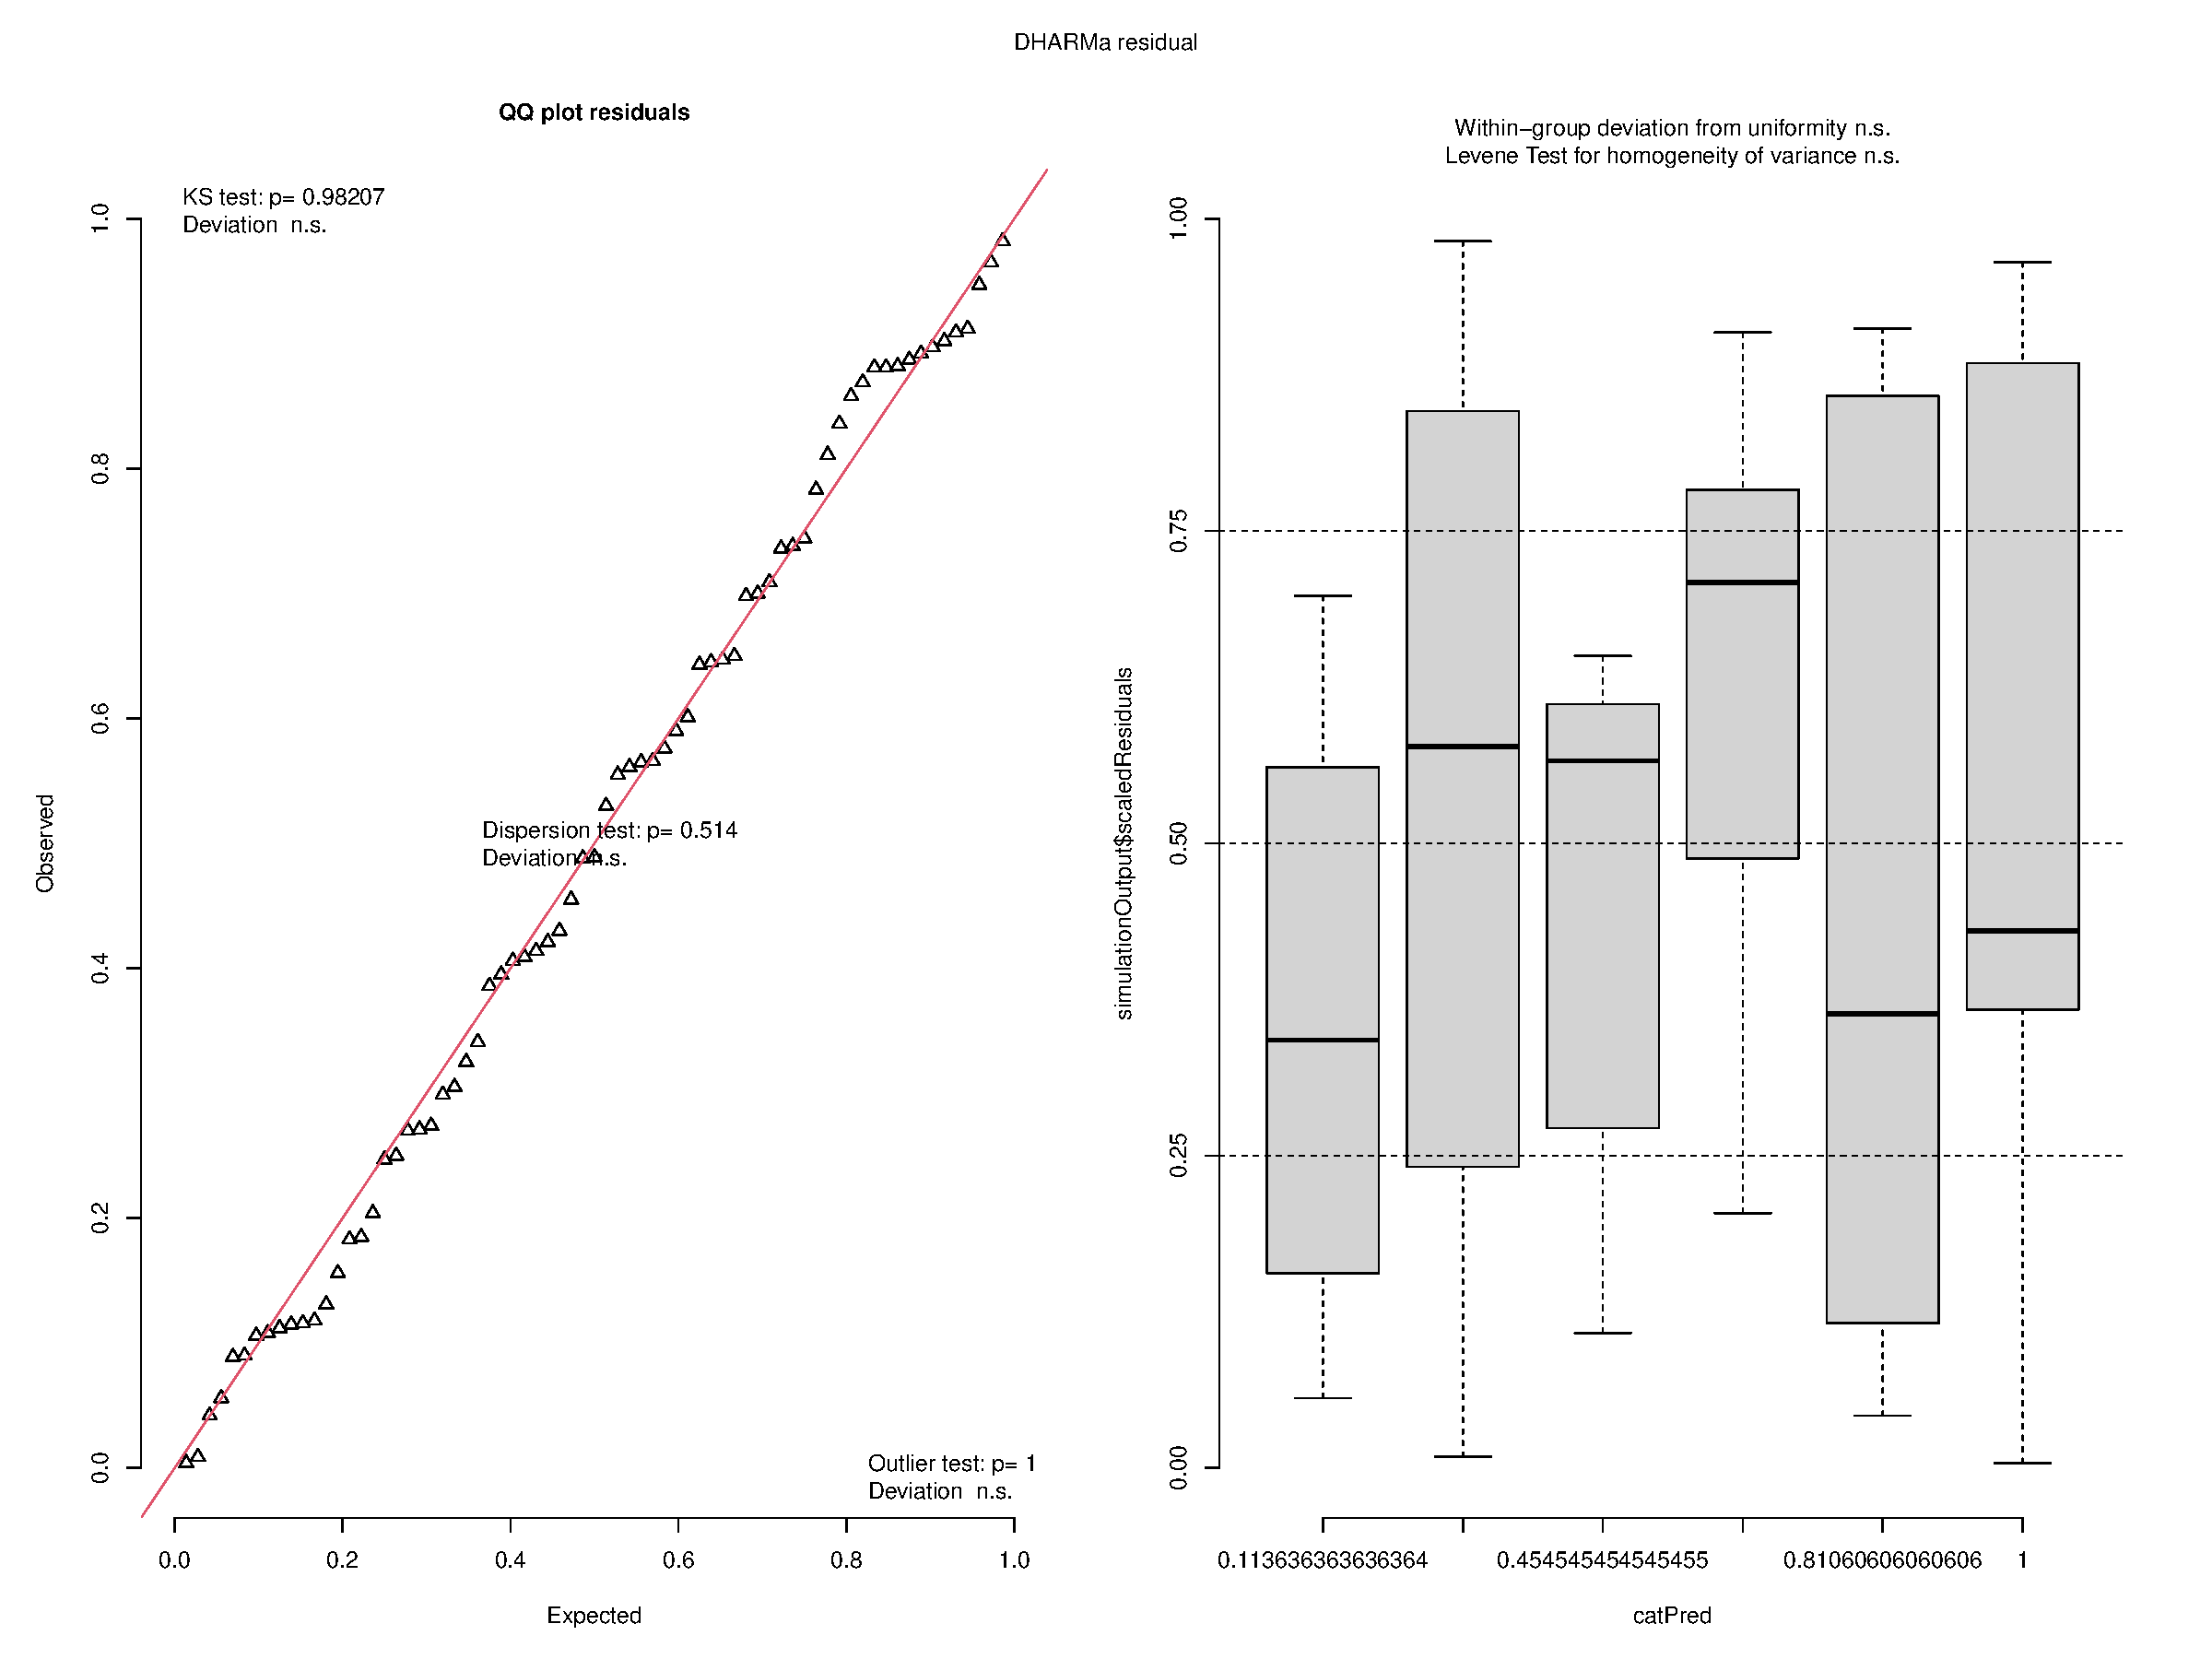
\includegraphics[keepaspectratio]{rsa_day1617_agar_files/figure-pdf/unnamed-chunk-5-6.pdf}}

\begin{Shaded}
\begin{Highlighting}[]
\FunctionTok{testUniformity}\NormalTok{(sim\_res)                     }\CommentTok{\# p \textgreater{} 0.05 = distribution correct}
\end{Highlighting}
\end{Shaded}

\pandocbounded{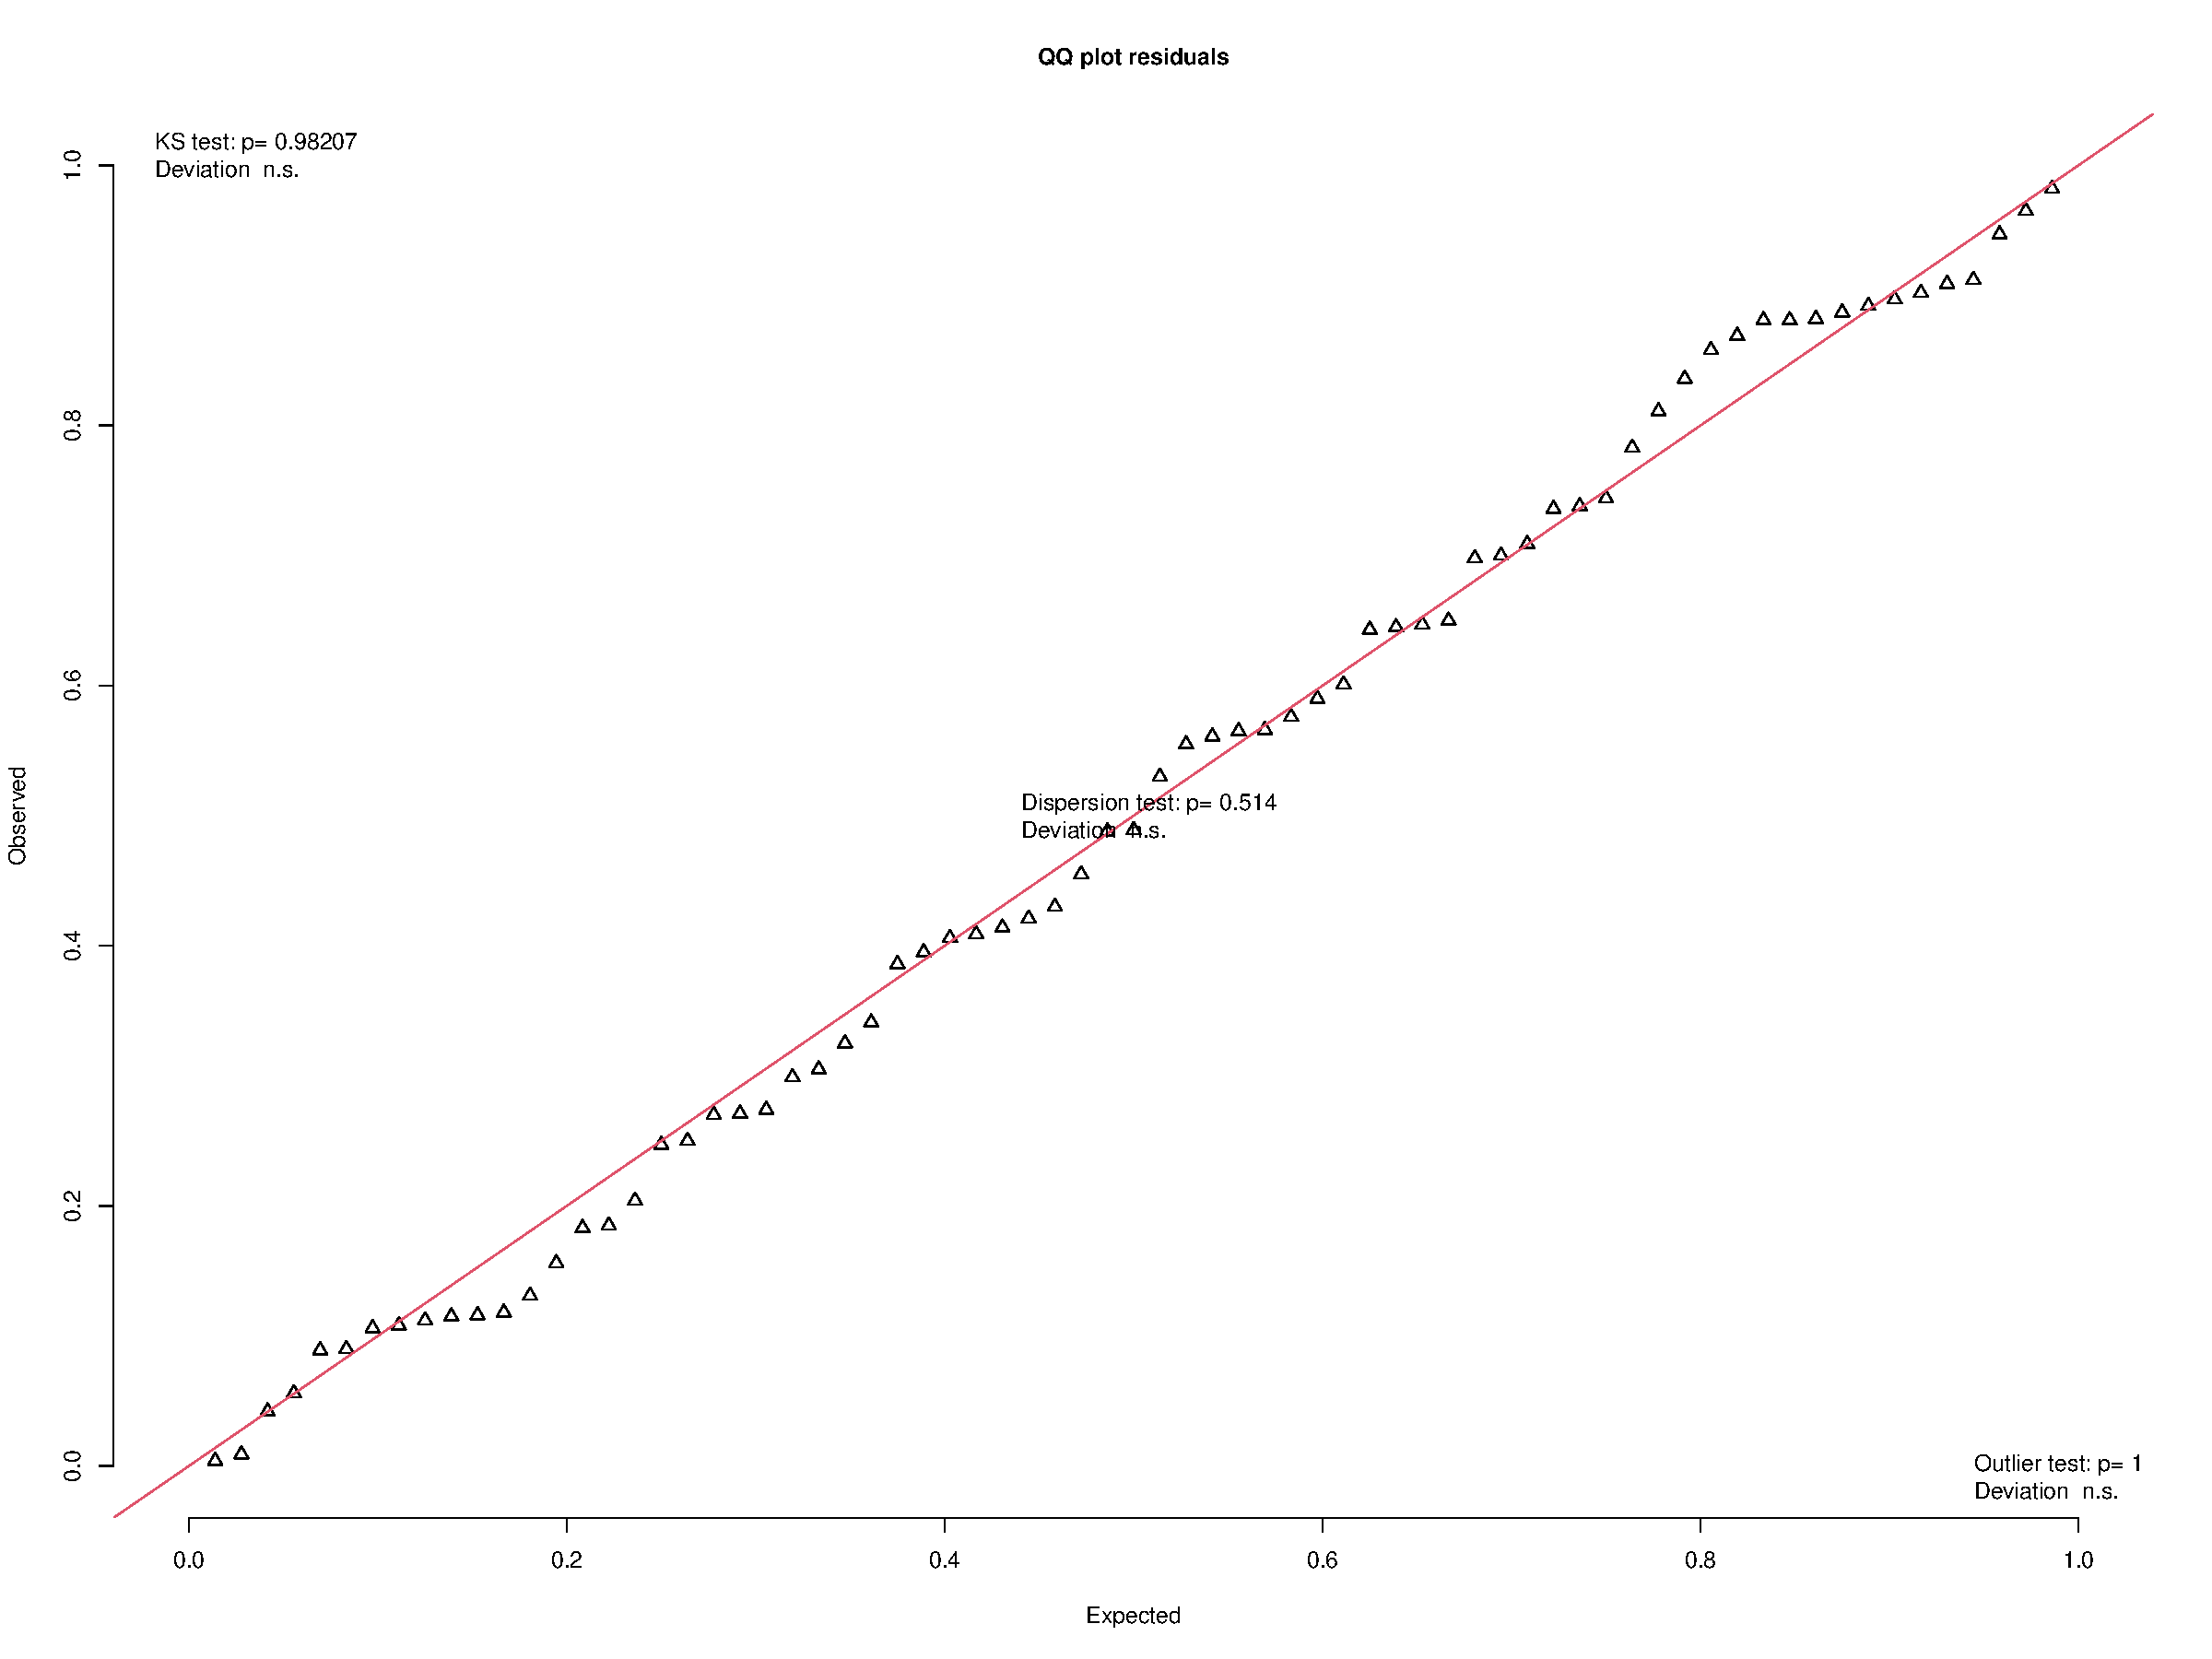
\includegraphics[keepaspectratio]{rsa_day1617_agar_files/figure-pdf/unnamed-chunk-5-7.pdf}}

\begin{verbatim}

    Asymptotic one-sample Kolmogorov-Smirnov test

data:  simulationOutput$scaledResiduals
D = 0.055183, p-value = 0.9821
alternative hypothesis: two-sided
\end{verbatim}

\begin{Shaded}
\begin{Highlighting}[]
\FunctionTok{testDispersion}\NormalTok{(sim\_res)                     }\CommentTok{\# ratio ≈ 1.0}
\end{Highlighting}
\end{Shaded}

\pandocbounded{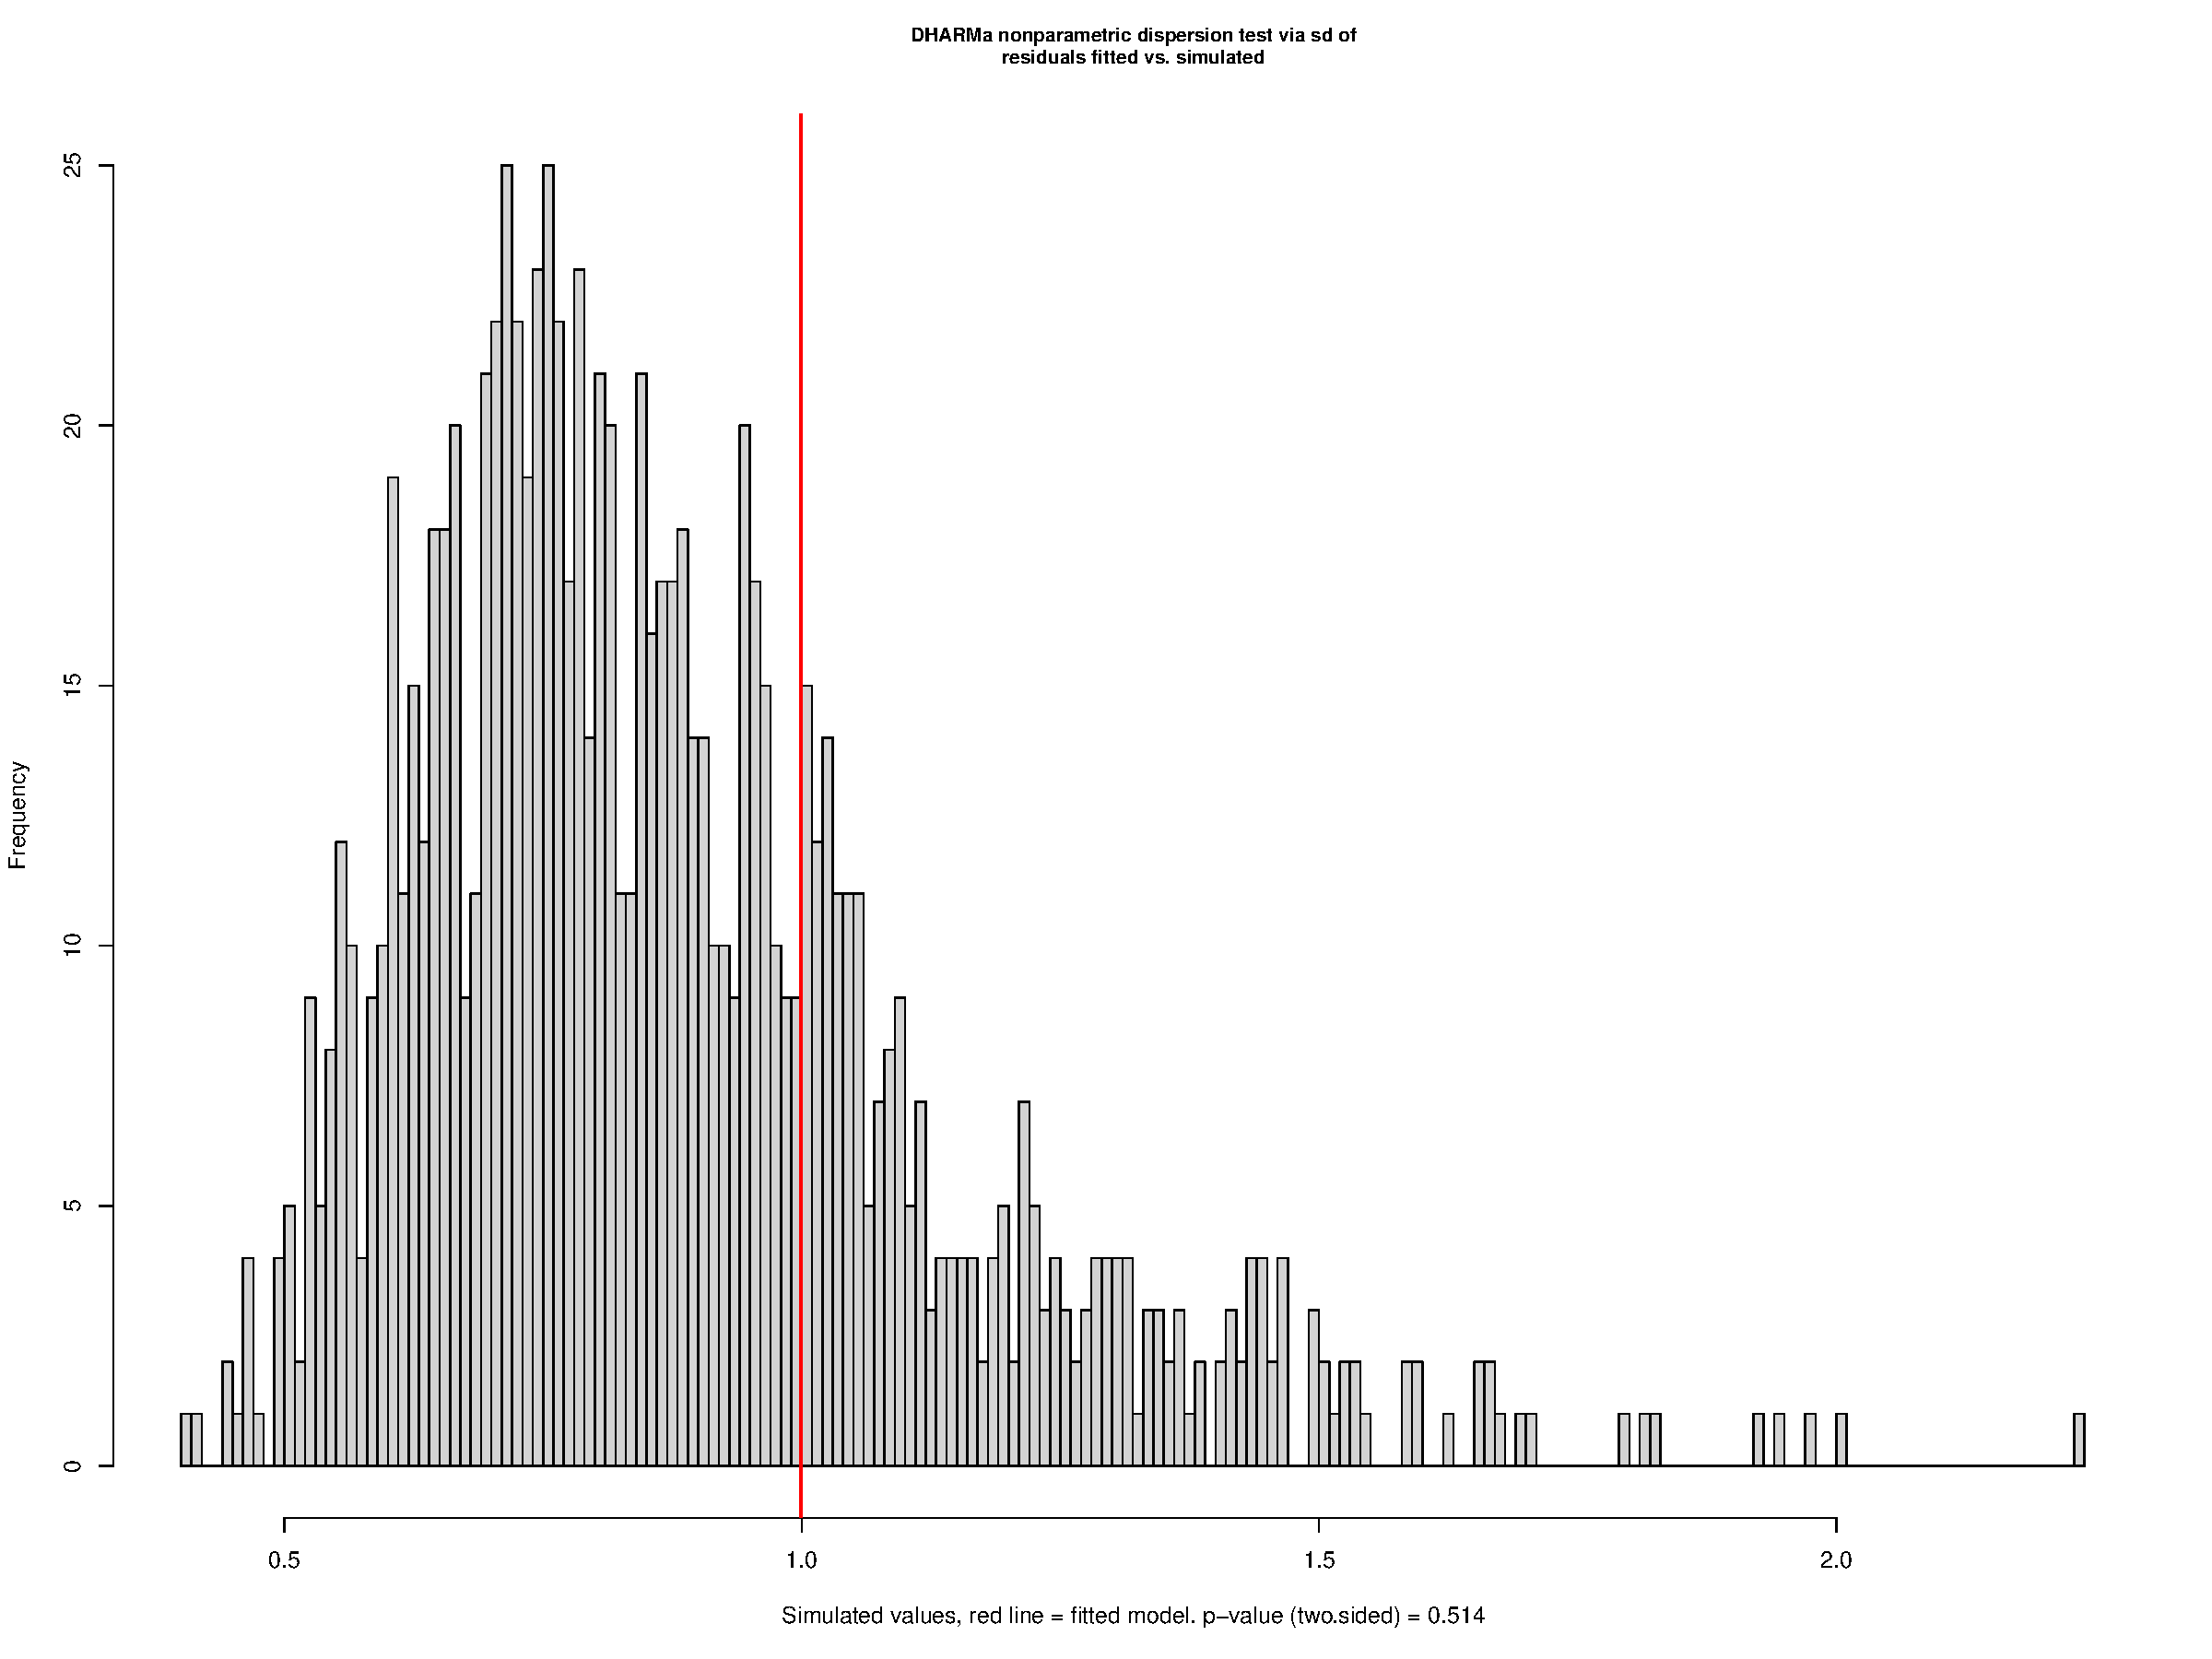
\includegraphics[keepaspectratio]{rsa_day1617_agar_files/figure-pdf/unnamed-chunk-5-8.pdf}}

\begin{verbatim}

    DHARMa nonparametric dispersion test via sd of residuals fitted vs.
    simulated

data:  simulationOutput
dispersion = 1.1371, p-value = 0.514
alternative hypothesis: two.sided
\end{verbatim}

\begin{Shaded}
\begin{Highlighting}[]
\FunctionTok{plotResiduals}\NormalTok{(sim\_res, }\AttributeTok{form =}\NormalTok{ df}\SpecialCharTok{$}\NormalTok{Genotype)  }\CommentTok{\# no patterns per genotype}
\end{Highlighting}
\end{Shaded}

\pandocbounded{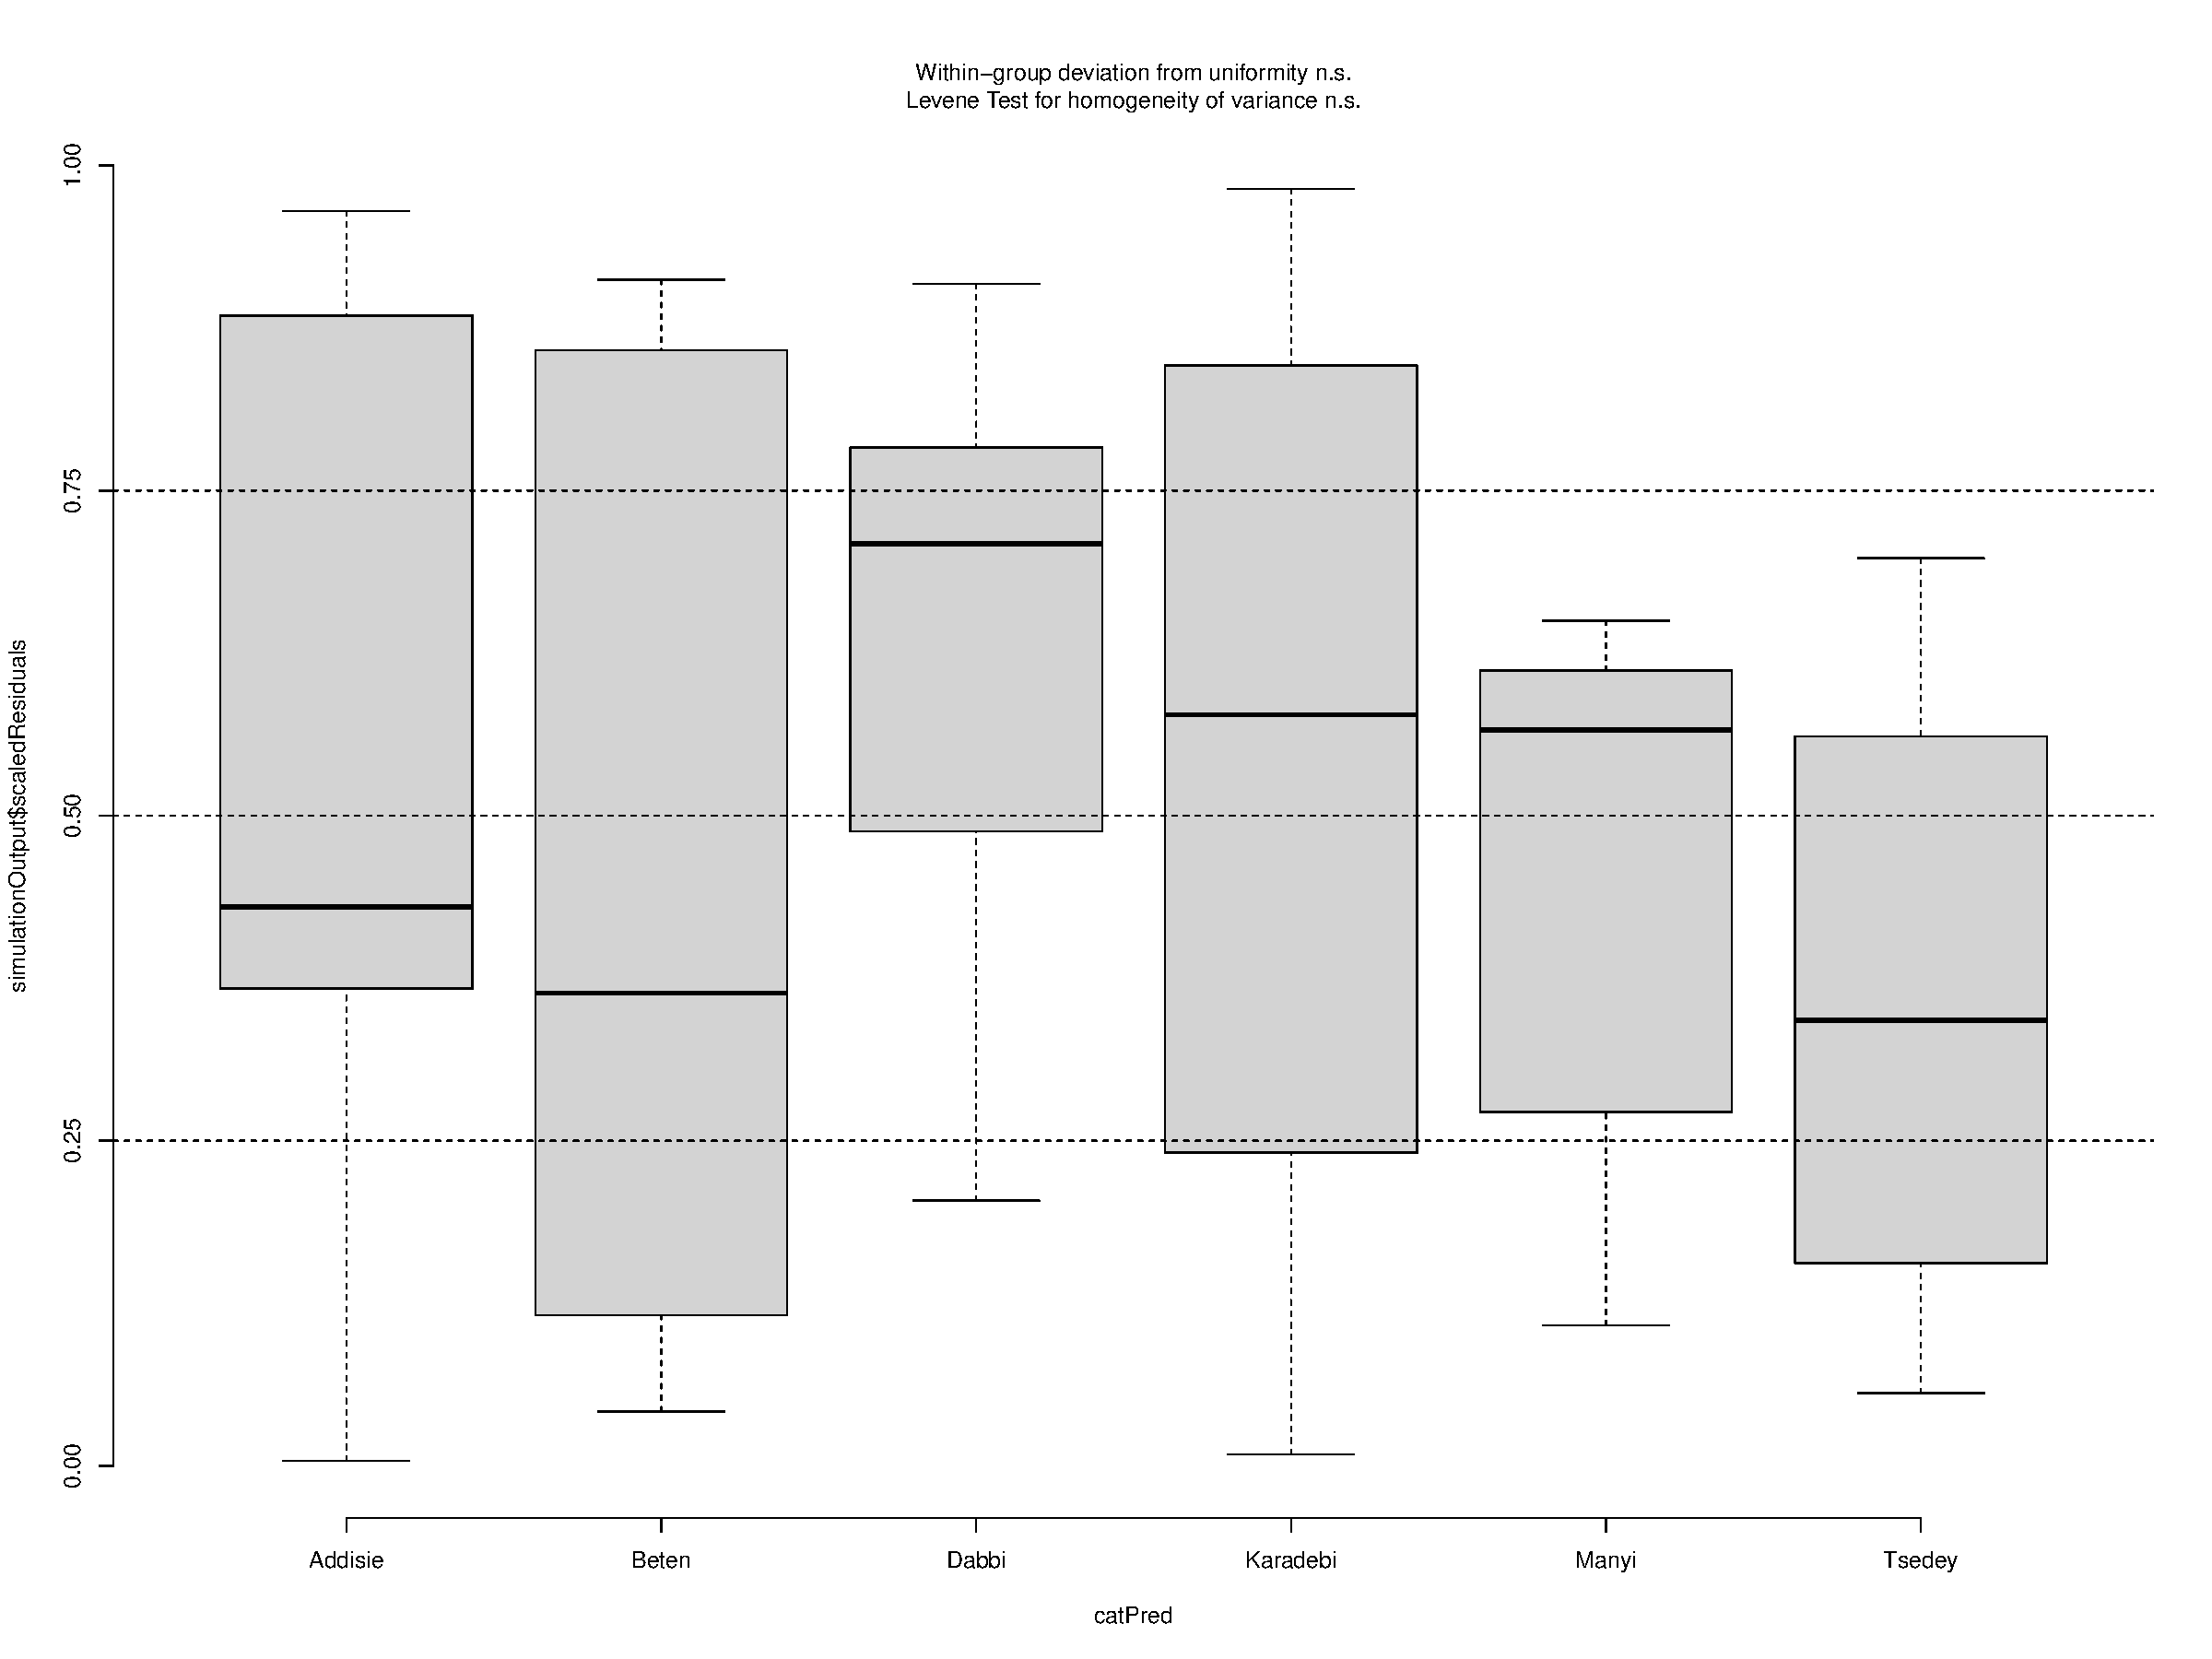
\includegraphics[keepaspectratio]{rsa_day1617_agar_files/figure-pdf/unnamed-chunk-5-9.pdf}}

\begin{Shaded}
\begin{Highlighting}[]
\CommentTok{\# imroved fit so will keep this log transformed model }

\CommentTok{\# ── 5. Test overall Genotype effect ──────────────────────────}
\NormalTok{car}\SpecialCharTok{::}\FunctionTok{Anova}\NormalTok{(convex\_tmb, }\AttributeTok{type =} \StringTok{"III"}\NormalTok{)}
\end{Highlighting}
\end{Shaded}

\begin{verbatim}
Analysis of Deviance Table (Type III Wald chisquare tests)

Response: log(Convex.Area.mm2)
               Chisq Df Pr(>Chisq)    
(Intercept) 360.9809  1     <2e-16 ***
Genotype      3.8976  5     0.5642    
---
Signif. codes:  0 '***' 0.001 '**' 0.01 '*' 0.05 '.' 0.1 ' ' 1
\end{verbatim}

\begin{Shaded}
\begin{Highlighting}[]
\CommentTok{\# ── 6. Pairwise comparisons + CLD ────────────────────────────}
\NormalTok{emm }\OtherTok{\textless{}{-}} \FunctionTok{emmeans}\NormalTok{(convex\_tmb, }\SpecialCharTok{\textasciitilde{}}\NormalTok{ Genotype, }\AttributeTok{type =} \StringTok{"response"}\NormalTok{)}
\FunctionTok{pairs}\NormalTok{(emm, }\AttributeTok{adjust =} \StringTok{"sidak"}\NormalTok{)}
\end{Highlighting}
\end{Shaded}

\begin{verbatim}
 contrast           ratio    SE  df null z.ratio p.value
 Addisie / Beten    1.057 0.287 Inf    1   0.206  1.0000
 Addisie / Dabbi    1.283 0.395 Inf    1   0.812  0.9997
 Addisie / Karadebi 1.311 0.404 Inf    1   0.878  0.9992
 Addisie / Manyi    1.288 0.460 Inf    1   0.708  0.9999
 Addisie / Tsedey   1.654 0.479 Inf    1   1.738  0.7236
 Beten / Dabbi      1.214 0.364 Inf    1   0.646  1.0000
 Beten / Karadebi   1.240 0.361 Inf    1   0.740  0.9999
 Beten / Manyi      1.218 0.415 Inf    1   0.578  1.0000
 Beten / Tsedey     1.564 0.419 Inf    1   1.668  0.7776
 Dabbi / Karadebi   1.022 0.286 Inf    1   0.076  1.0000
 Dabbi / Manyi      1.003 0.330 Inf    1   0.010  1.0000
 Dabbi / Tsedey     1.288 0.391 Inf    1   0.834  0.9996
 Karadebi / Manyi   0.982 0.318 Inf    1  -0.056  1.0000
 Karadebi / Tsedey  1.261 0.372 Inf    1   0.788  0.9998
 Manyi / Tsedey     1.284 0.420 Inf    1   0.765  0.9999

P value adjustment: sidak method for 15 tests 
Tests are performed on the log scale 
\end{verbatim}

\begin{Shaded}
\begin{Highlighting}[]
\NormalTok{cld\_df }\OtherTok{\textless{}{-}} \FunctionTok{as.data.frame}\NormalTok{(}\FunctionTok{cld}\NormalTok{(emm, }\AttributeTok{adjust =} \StringTok{"sidak"}\NormalTok{,}
                             \AttributeTok{Letters =}\NormalTok{ letters, }\AttributeTok{alpha =} \FloatTok{0.05}\NormalTok{)) }\SpecialCharTok{\%\textgreater{}\%}
  \FunctionTok{mutate}\NormalTok{(}\AttributeTok{.group =} \FunctionTok{trimws}\NormalTok{(.group))}

\NormalTok{n\_df }\OtherTok{\textless{}{-}}\NormalTok{ df }\SpecialCharTok{\%\textgreater{}\%}
  \FunctionTok{count}\NormalTok{(Genotype) }\SpecialCharTok{\%\textgreater{}\%}
  \FunctionTok{mutate}\NormalTok{(}\AttributeTok{label =} \FunctionTok{paste0}\NormalTok{(}\StringTok{"n="}\NormalTok{, n))}


\CommentTok{\# ── 7. Plot 1 — Boxplot ───────────────────────────────────────}

\NormalTok{y\_ceil }\OtherTok{\textless{}{-}} \FunctionTok{max}\NormalTok{(df}\SpecialCharTok{$}\NormalTok{Convex.Area.mm2) }\SpecialCharTok{*} \FloatTok{1.2}
\NormalTok{y\_label }\OtherTok{\textless{}{-}}\NormalTok{ y\_ceil }\SpecialCharTok{*} \FloatTok{0.87}

\NormalTok{p1 }\OtherTok{\textless{}{-}} \FunctionTok{ggplot}\NormalTok{(df, }\FunctionTok{aes}\NormalTok{(}\AttributeTok{x =}\NormalTok{ Genotype, }\AttributeTok{y =}\NormalTok{ Convex.Area.mm2, }\AttributeTok{fill =}\NormalTok{ Genotype)) }\SpecialCharTok{+}

  \FunctionTok{geom\_boxplot}\NormalTok{(}
    \AttributeTok{alpha =} \FloatTok{0.7}\NormalTok{, }\AttributeTok{outlier.shape =} \ConstantTok{NA}\NormalTok{,}
    \AttributeTok{width =} \FloatTok{0.5}\NormalTok{, }\AttributeTok{colour =} \StringTok{"black"}\NormalTok{, }\AttributeTok{linewidth =} \FloatTok{0.5}
\NormalTok{  ) }\SpecialCharTok{+}

  \FunctionTok{geom\_jitter}\NormalTok{(}\AttributeTok{width =} \FloatTok{0.15}\NormalTok{, }\AttributeTok{size =} \FloatTok{1.8}\NormalTok{, }\AttributeTok{alpha =} \FloatTok{0.55}\NormalTok{, }\AttributeTok{colour =} \StringTok{"black"}\NormalTok{) }\SpecialCharTok{+}

  \FunctionTok{geom\_text}\NormalTok{(}
    \AttributeTok{data =}\NormalTok{ cld\_df, }\FunctionTok{aes}\NormalTok{(}\AttributeTok{x =}\NormalTok{ Genotype, }\AttributeTok{label =}\NormalTok{ .group),}
    \AttributeTok{y =}\NormalTok{ y\_label, }\AttributeTok{inherit.aes =} \ConstantTok{FALSE}\NormalTok{,}
    \AttributeTok{size =} \DecValTok{5}\NormalTok{, }\AttributeTok{fontface =} \StringTok{"bold"}\NormalTok{, }\AttributeTok{colour =} \StringTok{"grey20"}
\NormalTok{  ) }\SpecialCharTok{+}

  \FunctionTok{geom\_text}\NormalTok{(}
    \AttributeTok{data =}\NormalTok{ n\_df, }\FunctionTok{aes}\NormalTok{(}\AttributeTok{x =}\NormalTok{ Genotype, }\AttributeTok{label =}\NormalTok{ label),}
    \AttributeTok{y =} \SpecialCharTok{{-}}\ConstantTok{Inf}\NormalTok{, }\AttributeTok{vjust =} \FloatTok{4.2}\NormalTok{, }\AttributeTok{inherit.aes =} \ConstantTok{FALSE}\NormalTok{,}
    \AttributeTok{size =} \FloatTok{3.5}\NormalTok{, }\AttributeTok{colour =} \StringTok{"grey40"}
\NormalTok{  ) }\SpecialCharTok{+}

  \FunctionTok{scale\_fill\_brewer}\NormalTok{(}\AttributeTok{palette =} \StringTok{"Set2"}\NormalTok{) }\SpecialCharTok{+}

  \FunctionTok{labs}\NormalTok{(}
    \AttributeTok{x       =} \StringTok{"Genotype"}\NormalTok{,}
    \AttributeTok{y       =} \FunctionTok{expression}\NormalTok{(Convex}\SpecialCharTok{\textasciitilde{}}\NormalTok{area}\SpecialCharTok{\textasciitilde{}}\NormalTok{(mm}\SpecialCharTok{\^{}}\DecValTok{2}\NormalTok{)),}
    \AttributeTok{caption =} \StringTok{"Shared letters indicate no significant difference (sidak HSD, p \textgreater{} 0.05; glmmTMB, Gaussian log)"}
\NormalTok{  ) }\SpecialCharTok{+}

  \FunctionTok{theme\_classic}\NormalTok{(}\AttributeTok{base\_size =} \DecValTok{14}\NormalTok{) }\SpecialCharTok{+}
  \FunctionTok{theme}\NormalTok{(}
    \AttributeTok{legend.position =} \StringTok{"none"}\NormalTok{,}
    \AttributeTok{axis.line       =} \FunctionTok{element\_line}\NormalTok{(}\AttributeTok{colour =} \StringTok{"black"}\NormalTok{, }\AttributeTok{linewidth =} \FloatTok{0.6}\NormalTok{),}
    \AttributeTok{axis.ticks      =} \FunctionTok{element\_line}\NormalTok{(}\AttributeTok{colour =} \StringTok{"black"}\NormalTok{, }\AttributeTok{linewidth =} \FloatTok{0.5}\NormalTok{),}
    \AttributeTok{axis.title      =} \FunctionTok{element\_text}\NormalTok{(}\AttributeTok{size =} \DecValTok{14}\NormalTok{, }\AttributeTok{face =} \StringTok{"bold"}\NormalTok{),}
    \AttributeTok{axis.text       =} \FunctionTok{element\_text}\NormalTok{(}\AttributeTok{size =} \DecValTok{14}\NormalTok{, }\AttributeTok{colour =} \StringTok{"black"}\NormalTok{),}
    \AttributeTok{axis.text.x     =} \FunctionTok{element\_text}\NormalTok{(}\AttributeTok{face =} \StringTok{"italic"}\NormalTok{, }\AttributeTok{margin =} \FunctionTok{margin}\NormalTok{(}\AttributeTok{t =} \DecValTok{3}\NormalTok{)),}
    \AttributeTok{plot.caption    =} \FunctionTok{element\_text}\NormalTok{(}\AttributeTok{size =} \DecValTok{9}\NormalTok{, }\AttributeTok{colour =} \StringTok{"grey40"}\NormalTok{, }\AttributeTok{hjust =} \DecValTok{0}\NormalTok{),}
    \AttributeTok{plot.margin     =} \FunctionTok{margin}\NormalTok{(}\AttributeTok{t =} \DecValTok{10}\NormalTok{, }\AttributeTok{r =} \DecValTok{15}\NormalTok{, }\AttributeTok{b =} \DecValTok{30}\NormalTok{, }\AttributeTok{l =} \DecValTok{10}\NormalTok{)}
\NormalTok{  )}

\NormalTok{p1 }\SpecialCharTok{+} \FunctionTok{coord\_cartesian}\NormalTok{(}\AttributeTok{clip =} \StringTok{"off"}\NormalTok{)}
\end{Highlighting}
\end{Shaded}

\pandocbounded{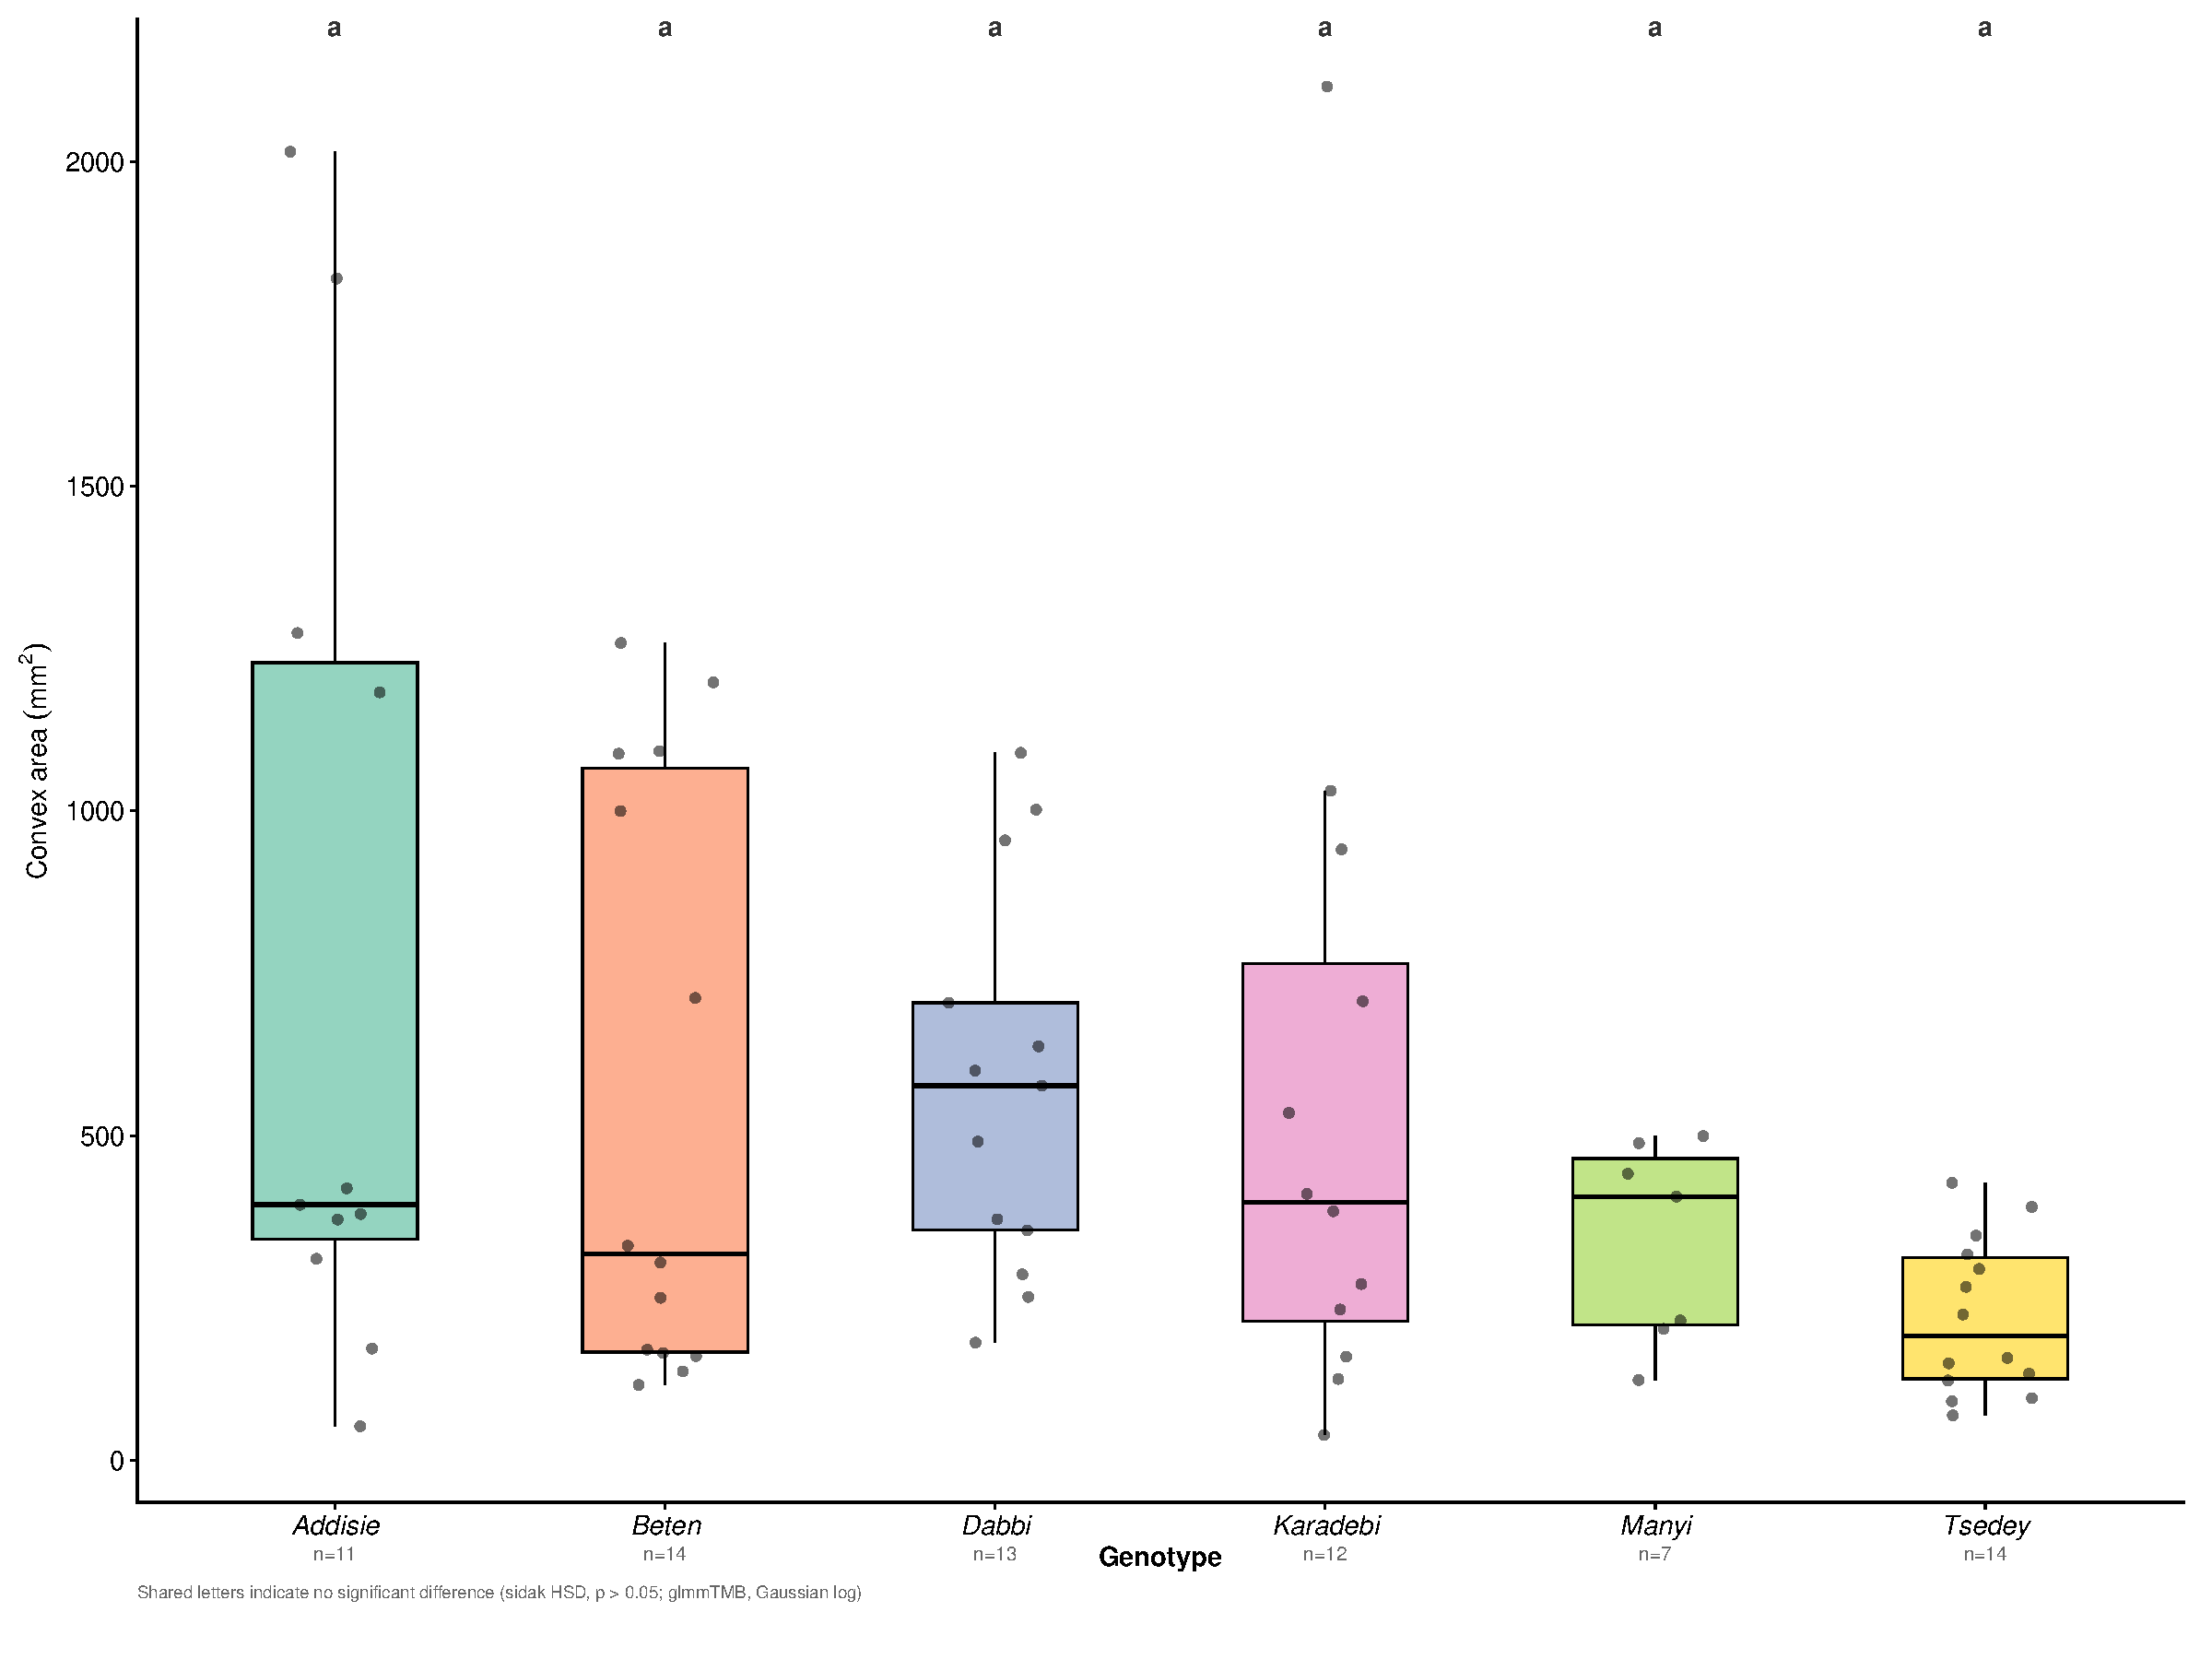
\includegraphics[keepaspectratio]{rsa_day1617_agar_files/figure-pdf/unnamed-chunk-5-10.pdf}}

\subsubsection{Network Area}\label{network-area}

\begin{Shaded}
\begin{Highlighting}[]
\CommentTok{\# ============================================================}
\CommentTok{\#  Network Area Analysis}
\CommentTok{\# ============================================================}

\CommentTok{\# ── 1. Inspect the trait ──────────────────────────────────────}
\FunctionTok{summary}\NormalTok{(df}\SpecialCharTok{$}\NormalTok{Network.Area.mm2)}
\end{Highlighting}
\end{Shaded}

\begin{verbatim}
   Min. 1st Qu.  Median    Mean 3rd Qu.    Max. 
  8.655  16.985  24.994  30.207  38.181 101.103 
\end{verbatim}

\begin{Shaded}
\begin{Highlighting}[]
\FunctionTok{hist}\NormalTok{(df}\SpecialCharTok{$}\NormalTok{Network.Area.mm2, }\AttributeTok{breaks =} \DecValTok{15}\NormalTok{, }\AttributeTok{main =} \StringTok{"Network Area distribution"}\NormalTok{)}
\end{Highlighting}
\end{Shaded}

\pandocbounded{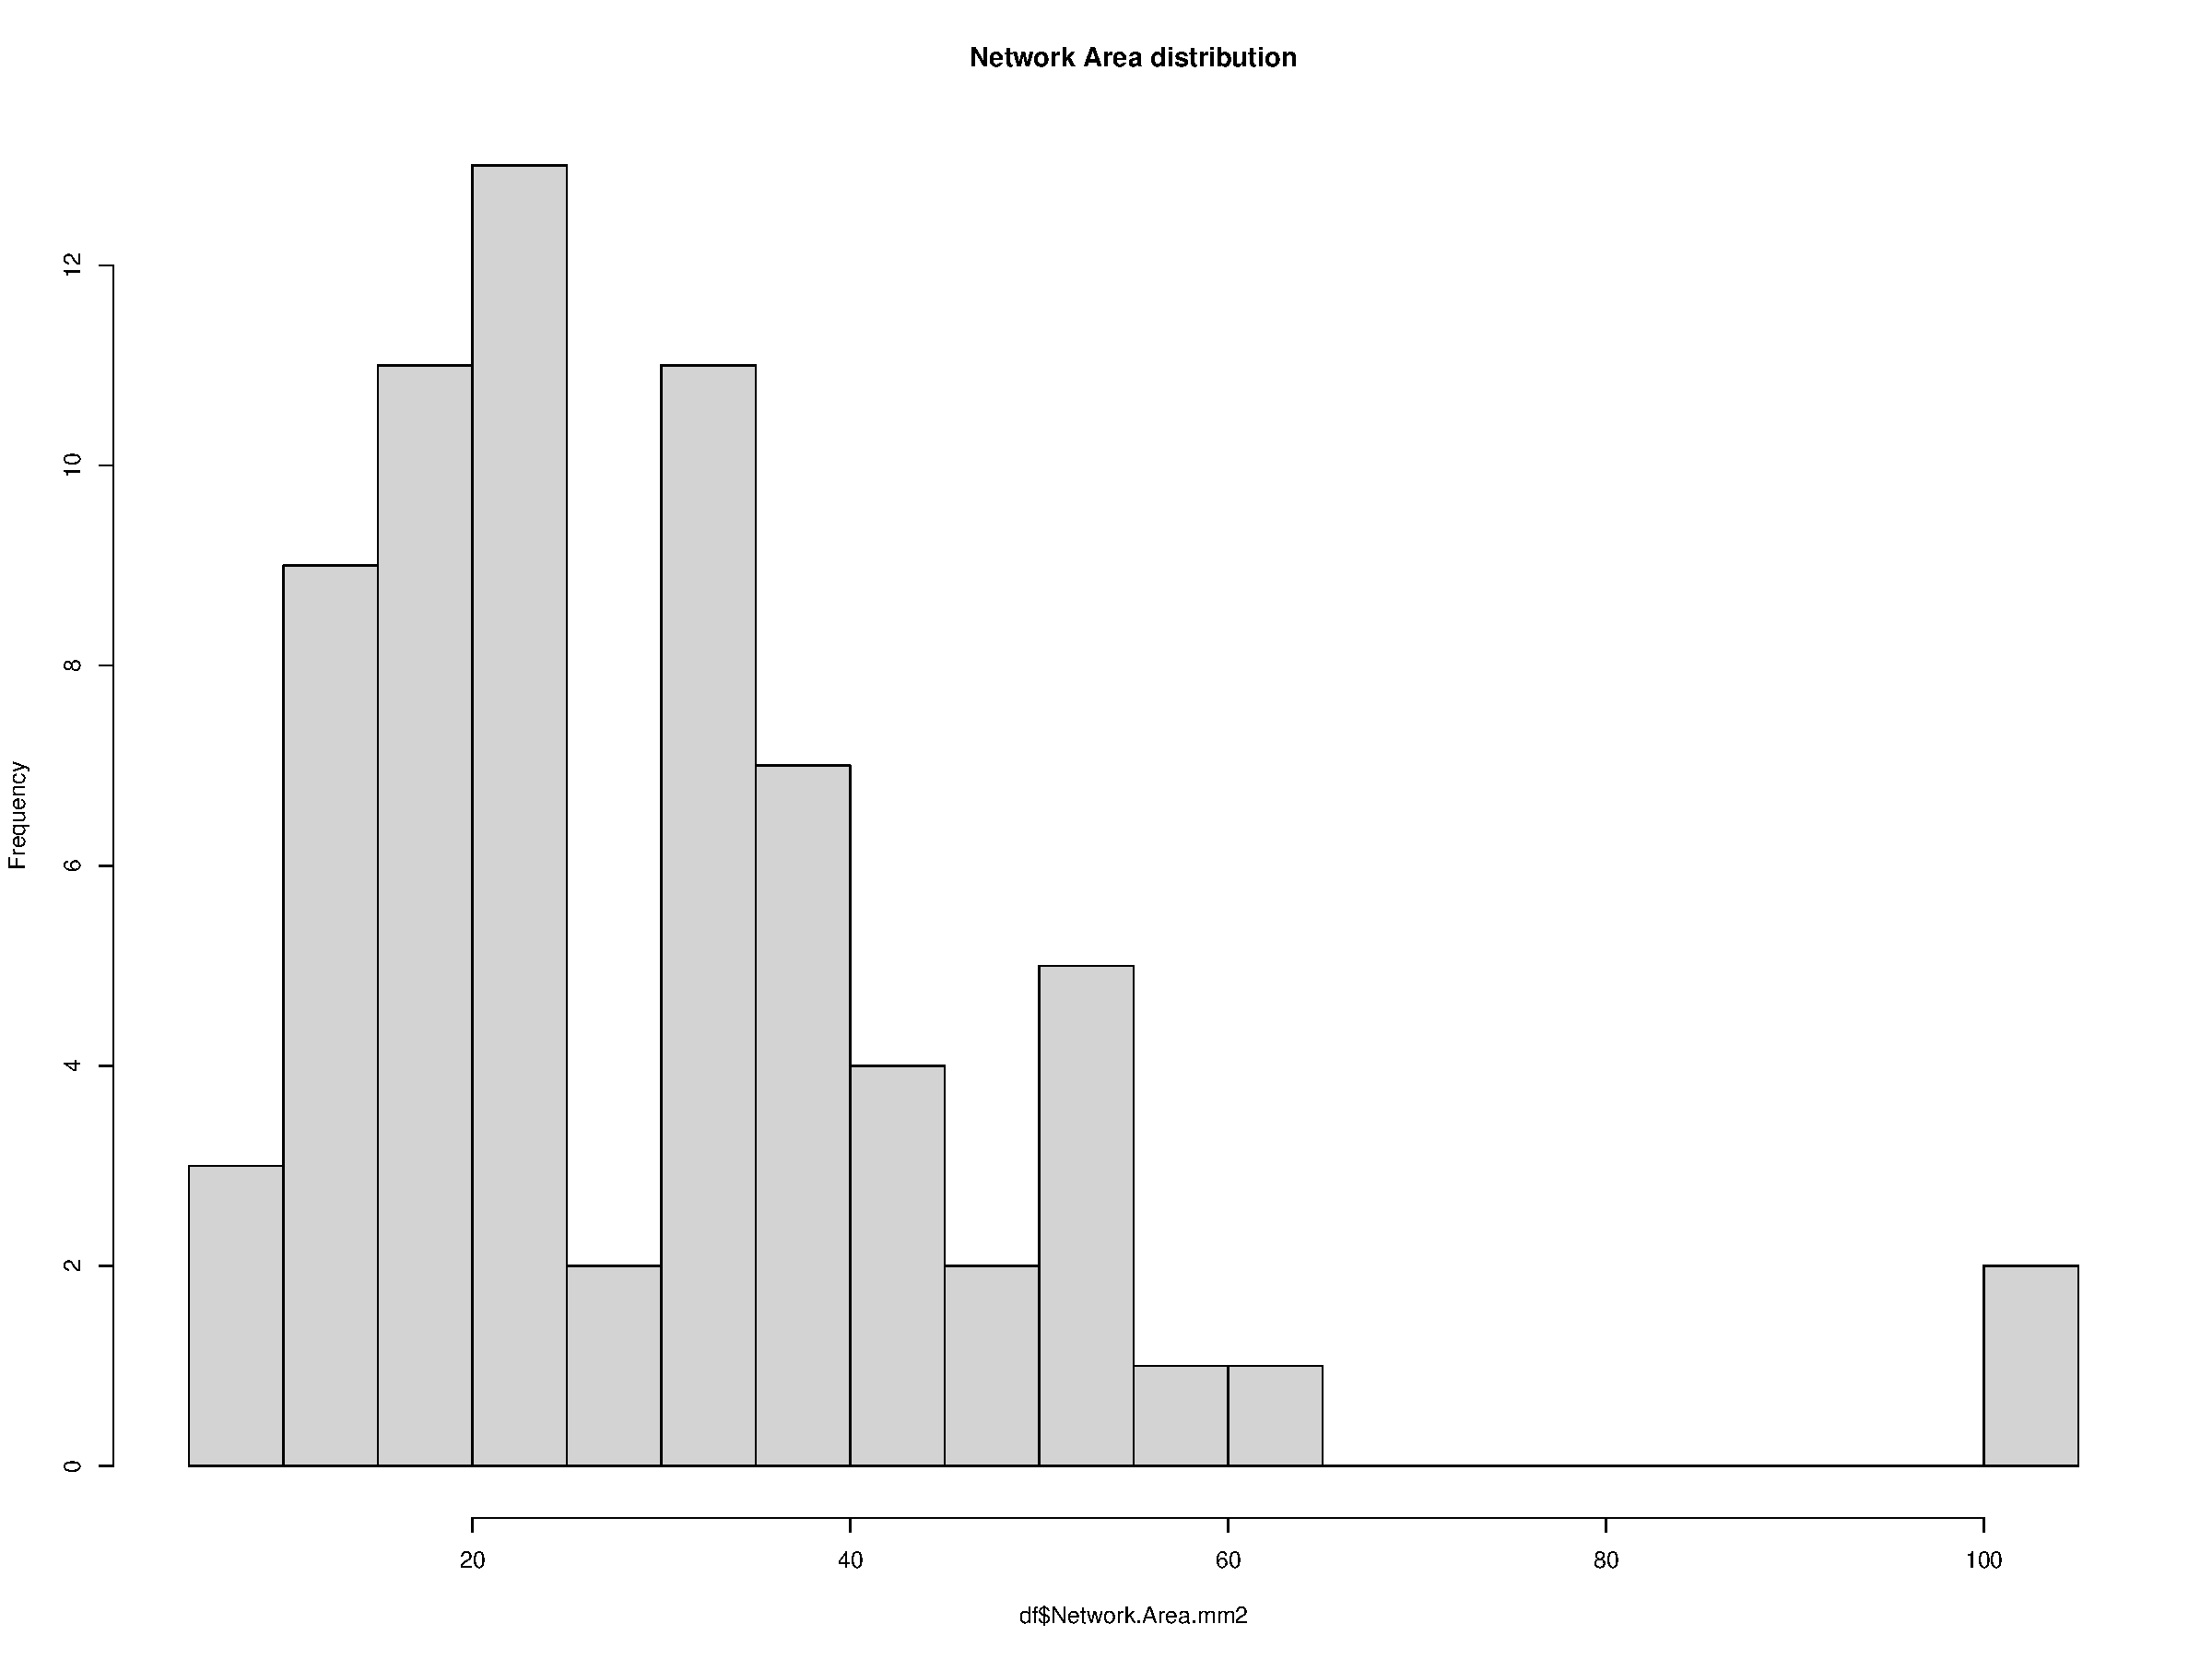
\includegraphics[keepaspectratio]{rsa_day1617_agar_files/figure-pdf/unnamed-chunk-6-1.pdf}}

\begin{Shaded}
\begin{Highlighting}[]
\CommentTok{\# ── 2. Fit full nested model first ───────────────────────────}
\NormalTok{network\_full }\OtherTok{\textless{}{-}} \FunctionTok{glmmTMB}\NormalTok{(}
\NormalTok{  (Network.Area.mm2) }\SpecialCharTok{\textasciitilde{}}\NormalTok{ Genotype }\SpecialCharTok{+}\NormalTok{ (}\DecValTok{1} \SpecialCharTok{|}\NormalTok{ Batch}\SpecialCharTok{/}\NormalTok{Plate}\SpecialCharTok{/}\NormalTok{Seed),}
  \AttributeTok{data =}\NormalTok{ df, }\AttributeTok{family =} \FunctionTok{gaussian}\NormalTok{()}
\NormalTok{)}
\end{Highlighting}
\end{Shaded}

\begin{verbatim}
Warning in finalizeTMB(TMBStruc, obj, fit, h, data.tmb.old): Model convergence
problem; non-positive-definite Hessian matrix. See vignette('troubleshooting')
\end{verbatim}

\begin{Shaded}
\begin{Highlighting}[]
\FunctionTok{VarCorr}\NormalTok{(network\_full)}
\end{Highlighting}
\end{Shaded}

\begin{verbatim}

Conditional model:
 Groups           Name        Std.Dev. 
 Seed:Plate:Batch (Intercept)  4.514304
 Plate:Batch      (Intercept)  0.035244
 Batch            (Intercept)  7.935842
 Residual                     13.864816
\end{verbatim}

\begin{Shaded}
\begin{Highlighting}[]
\FunctionTok{check\_singularity}\NormalTok{(network\_full)}
\end{Highlighting}
\end{Shaded}

\begin{verbatim}
[1] FALSE
\end{verbatim}

\begin{Shaded}
\begin{Highlighting}[]
\FunctionTok{summary}\NormalTok{(network\_full)}
\end{Highlighting}
\end{Shaded}

\begin{verbatim}
 Family: gaussian  ( identity )
Formula:          (Network.Area.mm2) ~ Genotype + (1 | Batch/Plate/Seed)
Data: df

      AIC       BIC    logLik -2*log(L)  df.resid 
       NA        NA        NA        NA        61 

Random effects:

Conditional model:
 Groups           Name        Variance  Std.Dev.
 Seed:Plate:Batch (Intercept) 2.038e+01  4.51430
 Plate:Batch      (Intercept) 1.242e-03  0.03524
 Batch            (Intercept) 6.298e+01  7.93584
 Residual                     1.922e+02 13.86482
Number of obs: 71, groups:  Seed:Plate:Batch, 38; Plate:Batch, 18; Batch, 4

Dispersion estimate for gaussian family (sigma^2):  192 

Conditional model:
                 Estimate Std. Error z value Pr(>|z|)    
(Intercept)        36.494      6.093   5.989 2.11e-09 ***
GenotypeBeten      -5.616      5.776  -0.972   0.3310    
GenotypeDabbi      -7.703      6.731  -1.144   0.2524    
GenotypeKaradebi   -2.718      6.566  -0.414   0.6789    
GenotypeManyi      -4.468      7.760  -0.576   0.5648    
GenotypeTsedey    -15.541      6.243  -2.489   0.0128 *  
---
Signif. codes:  0 '***' 0.001 '**' 0.01 '*' 0.05 '.' 0.1 ' ' 1
\end{verbatim}

\begin{Shaded}
\begin{Highlighting}[]
\CommentTok{\# Standard deviation is incredibly small for plate:batch so getting the Hessian matrix error so will use a model which drops this interaction}


\CommentTok{\# ── 3. Simplified model (use if full model fails) ─────────────}
\NormalTok{network\_tmb }\OtherTok{\textless{}{-}} \FunctionTok{glmmTMB}\NormalTok{(}
\NormalTok{  Network.Area.mm2 }\SpecialCharTok{\textasciitilde{}}\NormalTok{ Genotype }\SpecialCharTok{+}\NormalTok{ (}\DecValTok{1} \SpecialCharTok{|}\NormalTok{ Batch) }\SpecialCharTok{+}\NormalTok{ (}\DecValTok{1} \SpecialCharTok{|}\NormalTok{ Seed}\SpecialCharTok{:}\NormalTok{Plate}\SpecialCharTok{:}\NormalTok{Batch),}
  \AttributeTok{data =}\NormalTok{ df, }\AttributeTok{family =} \FunctionTok{gaussian}\NormalTok{()}
\NormalTok{)}

\FunctionTok{VarCorr}\NormalTok{(network\_tmb)}
\end{Highlighting}
\end{Shaded}

\begin{verbatim}

Conditional model:
 Groups           Name        Std.Dev.
 Batch            (Intercept)  7.9362 
 Seed:Plate:Batch (Intercept)  4.5145 
 Residual                     13.8648 
\end{verbatim}

\begin{Shaded}
\begin{Highlighting}[]
\FunctionTok{check\_singularity}\NormalTok{(network\_tmb)}
\end{Highlighting}
\end{Shaded}

\begin{verbatim}
[1] FALSE
\end{verbatim}

\begin{Shaded}
\begin{Highlighting}[]
\FunctionTok{summary}\NormalTok{(network\_tmb)   }\CommentTok{\# confirm real SEs and AIC}
\end{Highlighting}
\end{Shaded}

\begin{verbatim}
 Family: gaussian  ( identity )
Formula:          
Network.Area.mm2 ~ Genotype + (1 | Batch) + (1 | Seed:Plate:Batch)
Data: df

      AIC       BIC    logLik -2*log(L)  df.resid 
    606.4     626.8    -294.2     588.4        62 

Random effects:

Conditional model:
 Groups           Name        Variance Std.Dev.
 Batch            (Intercept)  62.98    7.936  
 Seed:Plate:Batch (Intercept)  20.38    4.514  
 Residual                     192.23   13.865  
Number of obs: 71, groups:  Batch, 4; Seed:Plate:Batch, 38

Dispersion estimate for gaussian family (sigma^2):  192 

Conditional model:
                 Estimate Std. Error z value Pr(>|z|)    
(Intercept)        36.494      6.094   5.989 2.11e-09 ***
GenotypeBeten      -5.615      5.776  -0.972   0.3310    
GenotypeDabbi      -7.703      6.731  -1.144   0.2524    
GenotypeKaradebi   -2.718      6.566  -0.414   0.6789    
GenotypeManyi      -4.468      7.760  -0.576   0.5648    
GenotypeTsedey    -15.541      6.243  -2.489   0.0128 *  
---
Signif. codes:  0 '***' 0.001 '**' 0.01 '*' 0.05 '.' 0.1 ' ' 1
\end{verbatim}

\begin{Shaded}
\begin{Highlighting}[]
\CommentTok{\# ── 4. Assumption checks ──────────────────────────────────────}
\NormalTok{sim\_res }\OtherTok{\textless{}{-}} \FunctionTok{simulateResiduals}\NormalTok{(network\_tmb, }\AttributeTok{n =} \DecValTok{1000}\NormalTok{)}
\FunctionTok{plot}\NormalTok{(sim\_res)}
\end{Highlighting}
\end{Shaded}

\pandocbounded{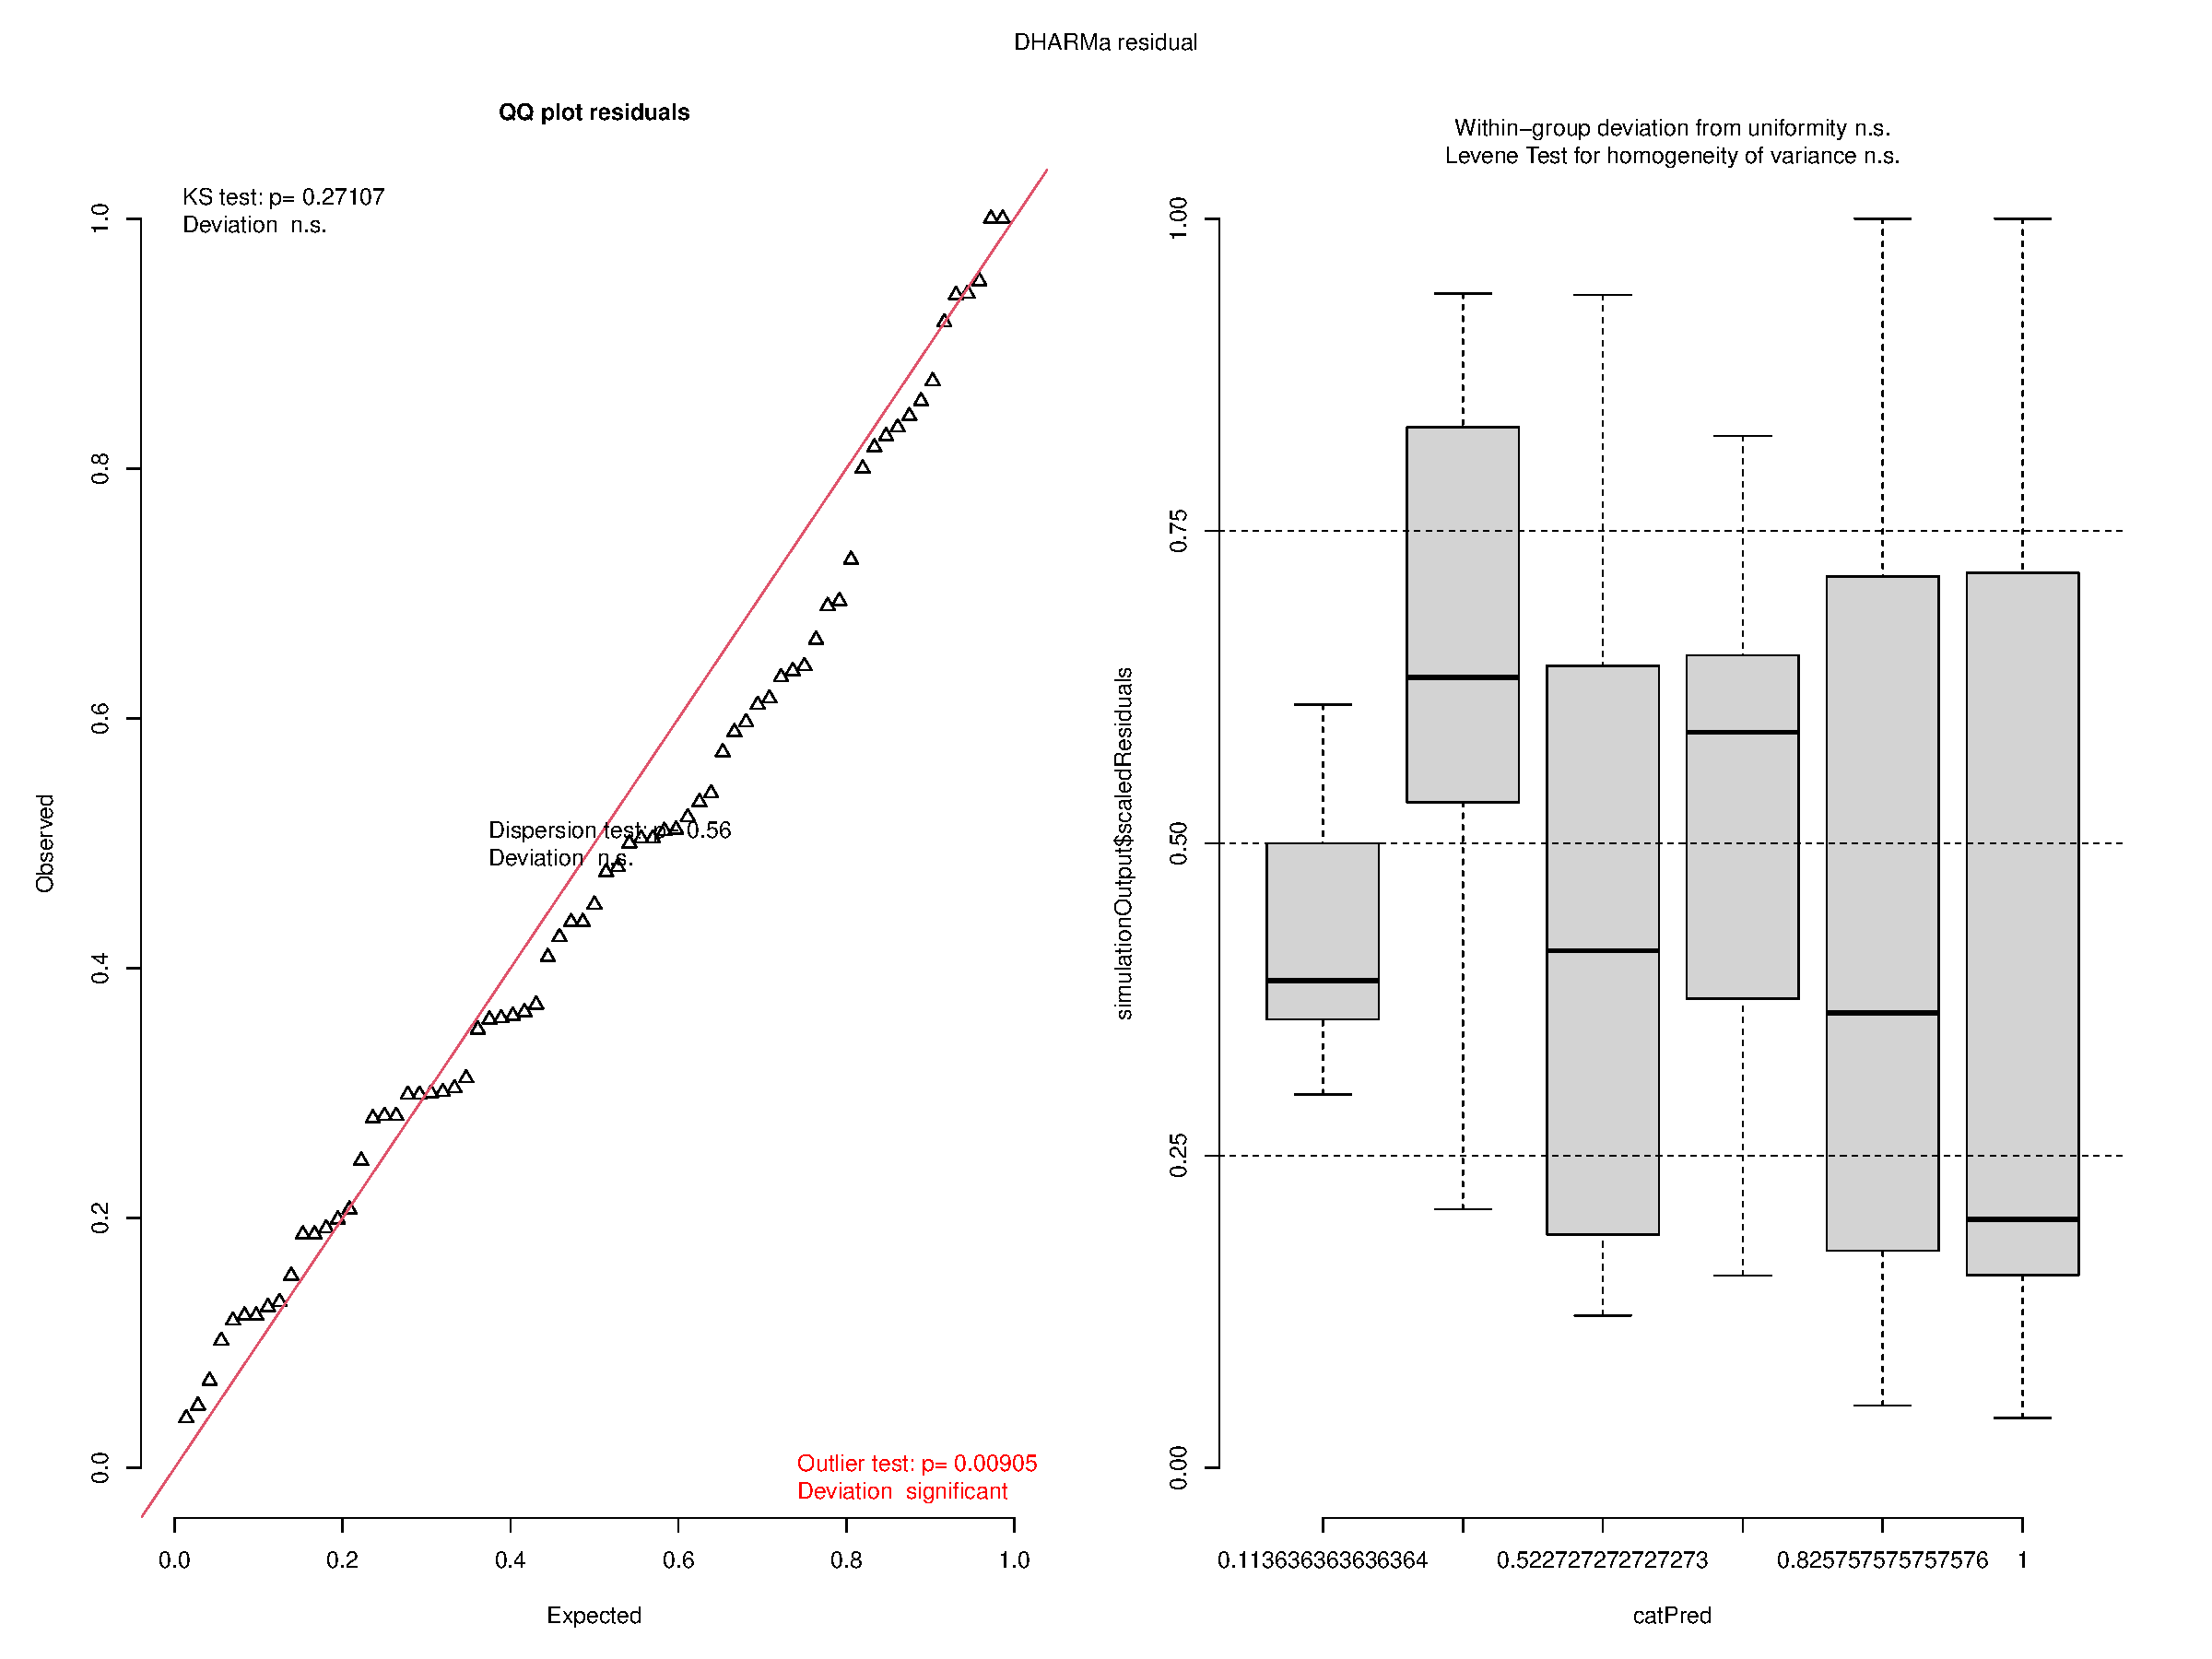
\includegraphics[keepaspectratio]{rsa_day1617_agar_files/figure-pdf/unnamed-chunk-6-2.pdf}}

\begin{Shaded}
\begin{Highlighting}[]
\FunctionTok{testUniformity}\NormalTok{(sim\_res)}
\end{Highlighting}
\end{Shaded}

\pandocbounded{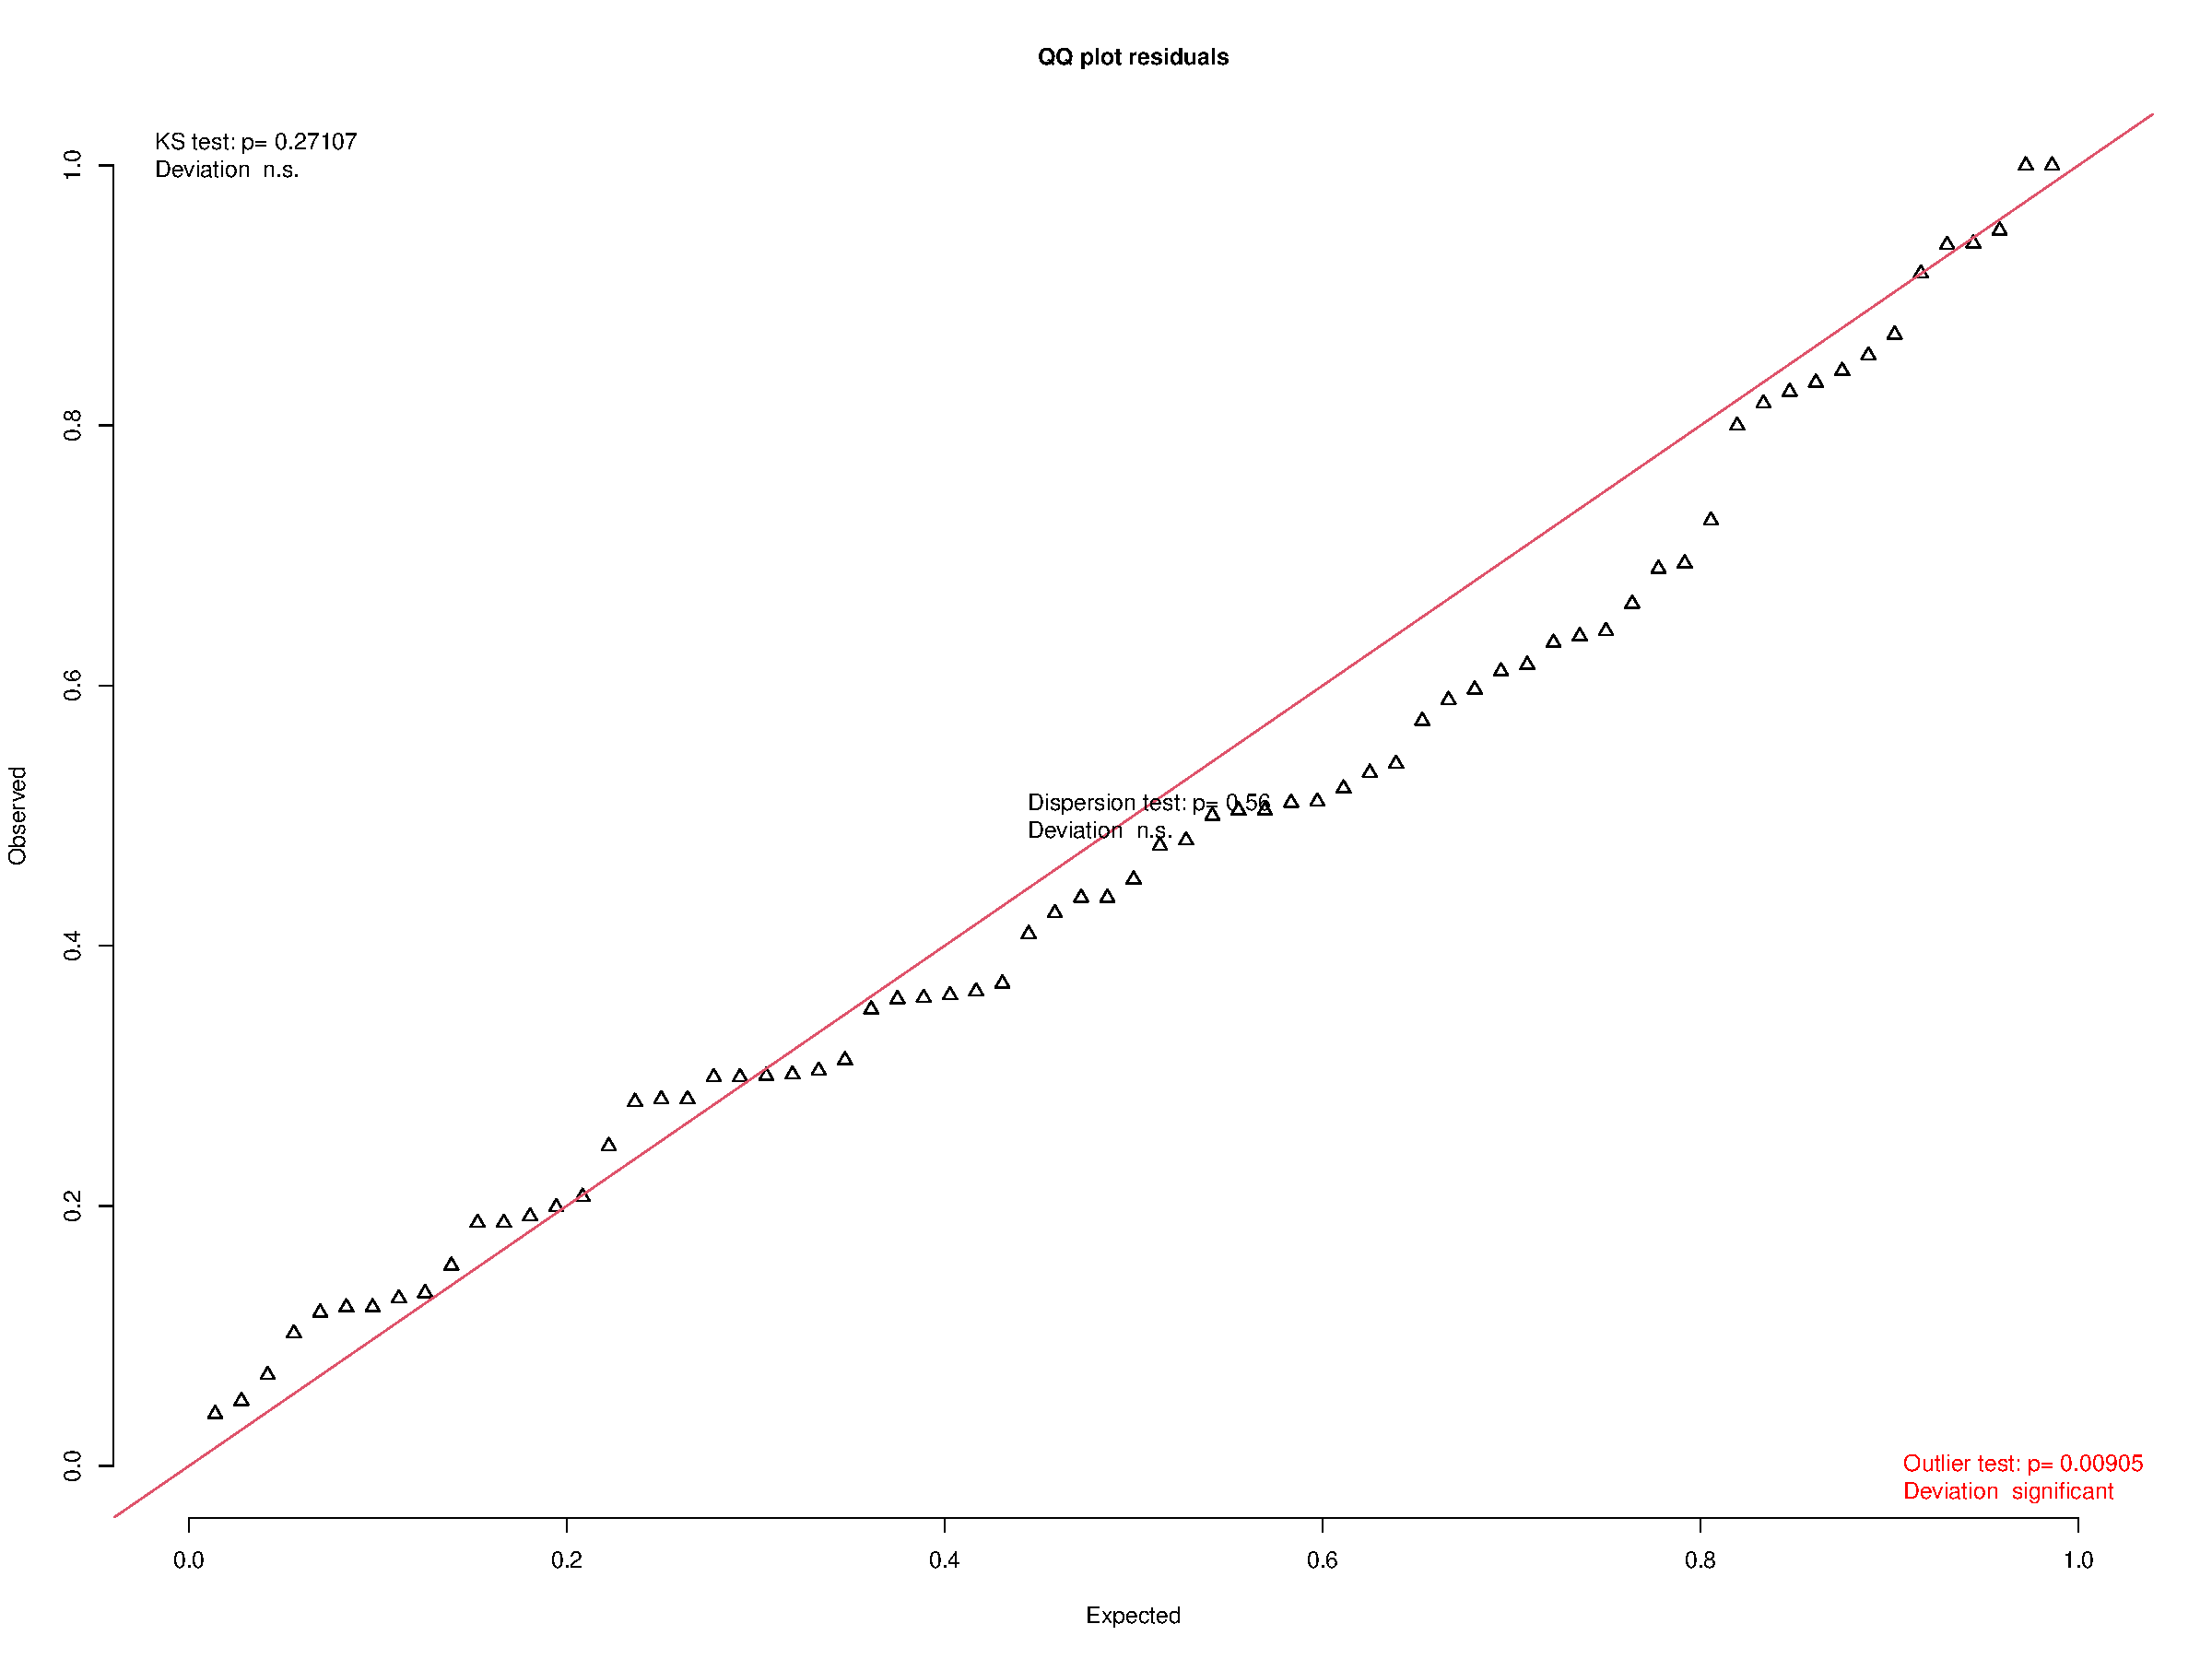
\includegraphics[keepaspectratio]{rsa_day1617_agar_files/figure-pdf/unnamed-chunk-6-3.pdf}}

\begin{verbatim}

    Asymptotic one-sample Kolmogorov-Smirnov test

data:  simulationOutput$scaledResiduals
D = 0.11856, p-value = 0.2711
alternative hypothesis: two-sided
\end{verbatim}

\begin{Shaded}
\begin{Highlighting}[]
\FunctionTok{testDispersion}\NormalTok{(sim\_res)}
\end{Highlighting}
\end{Shaded}

\pandocbounded{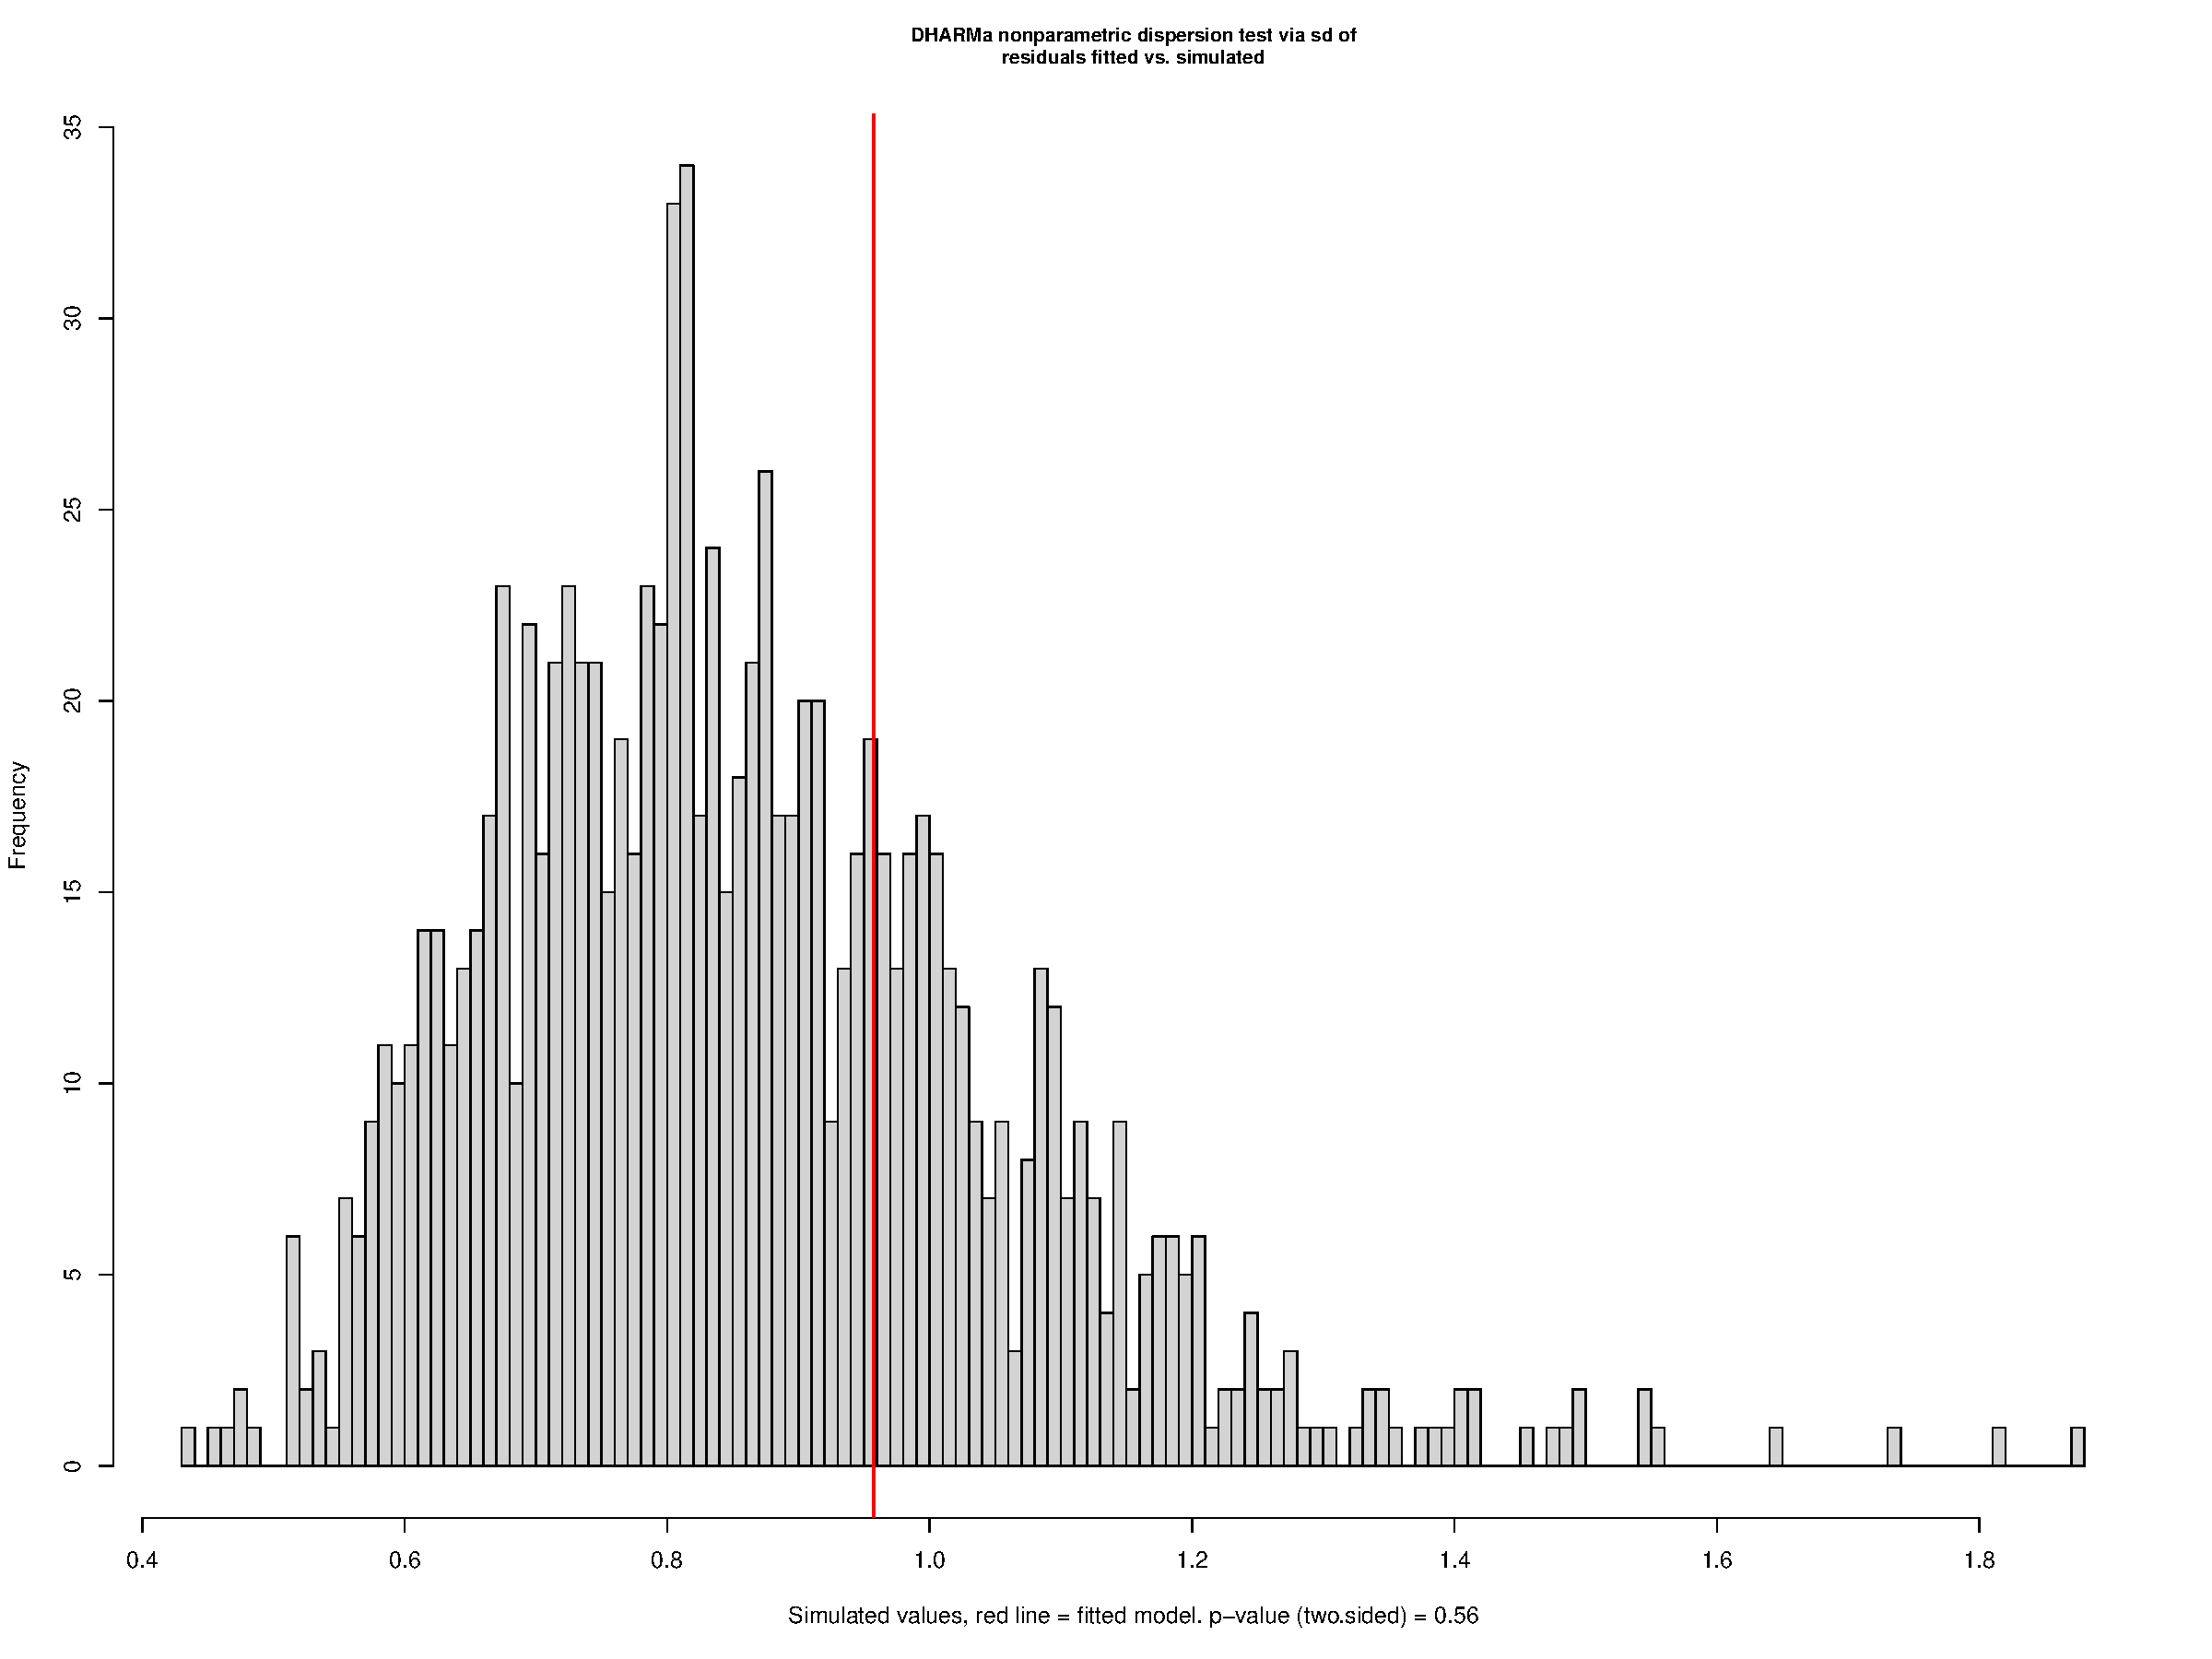
\includegraphics[keepaspectratio]{rsa_day1617_agar_files/figure-pdf/unnamed-chunk-6-4.pdf}}

\begin{verbatim}

    DHARMa nonparametric dispersion test via sd of residuals fitted vs.
    simulated

data:  simulationOutput
dispersion = 1.1119, p-value = 0.56
alternative hypothesis: two.sided
\end{verbatim}

\begin{Shaded}
\begin{Highlighting}[]
\FunctionTok{plotResiduals}\NormalTok{(sim\_res, }\AttributeTok{form =}\NormalTok{ df}\SpecialCharTok{$}\NormalTok{Genotype)}
\end{Highlighting}
\end{Shaded}

\pandocbounded{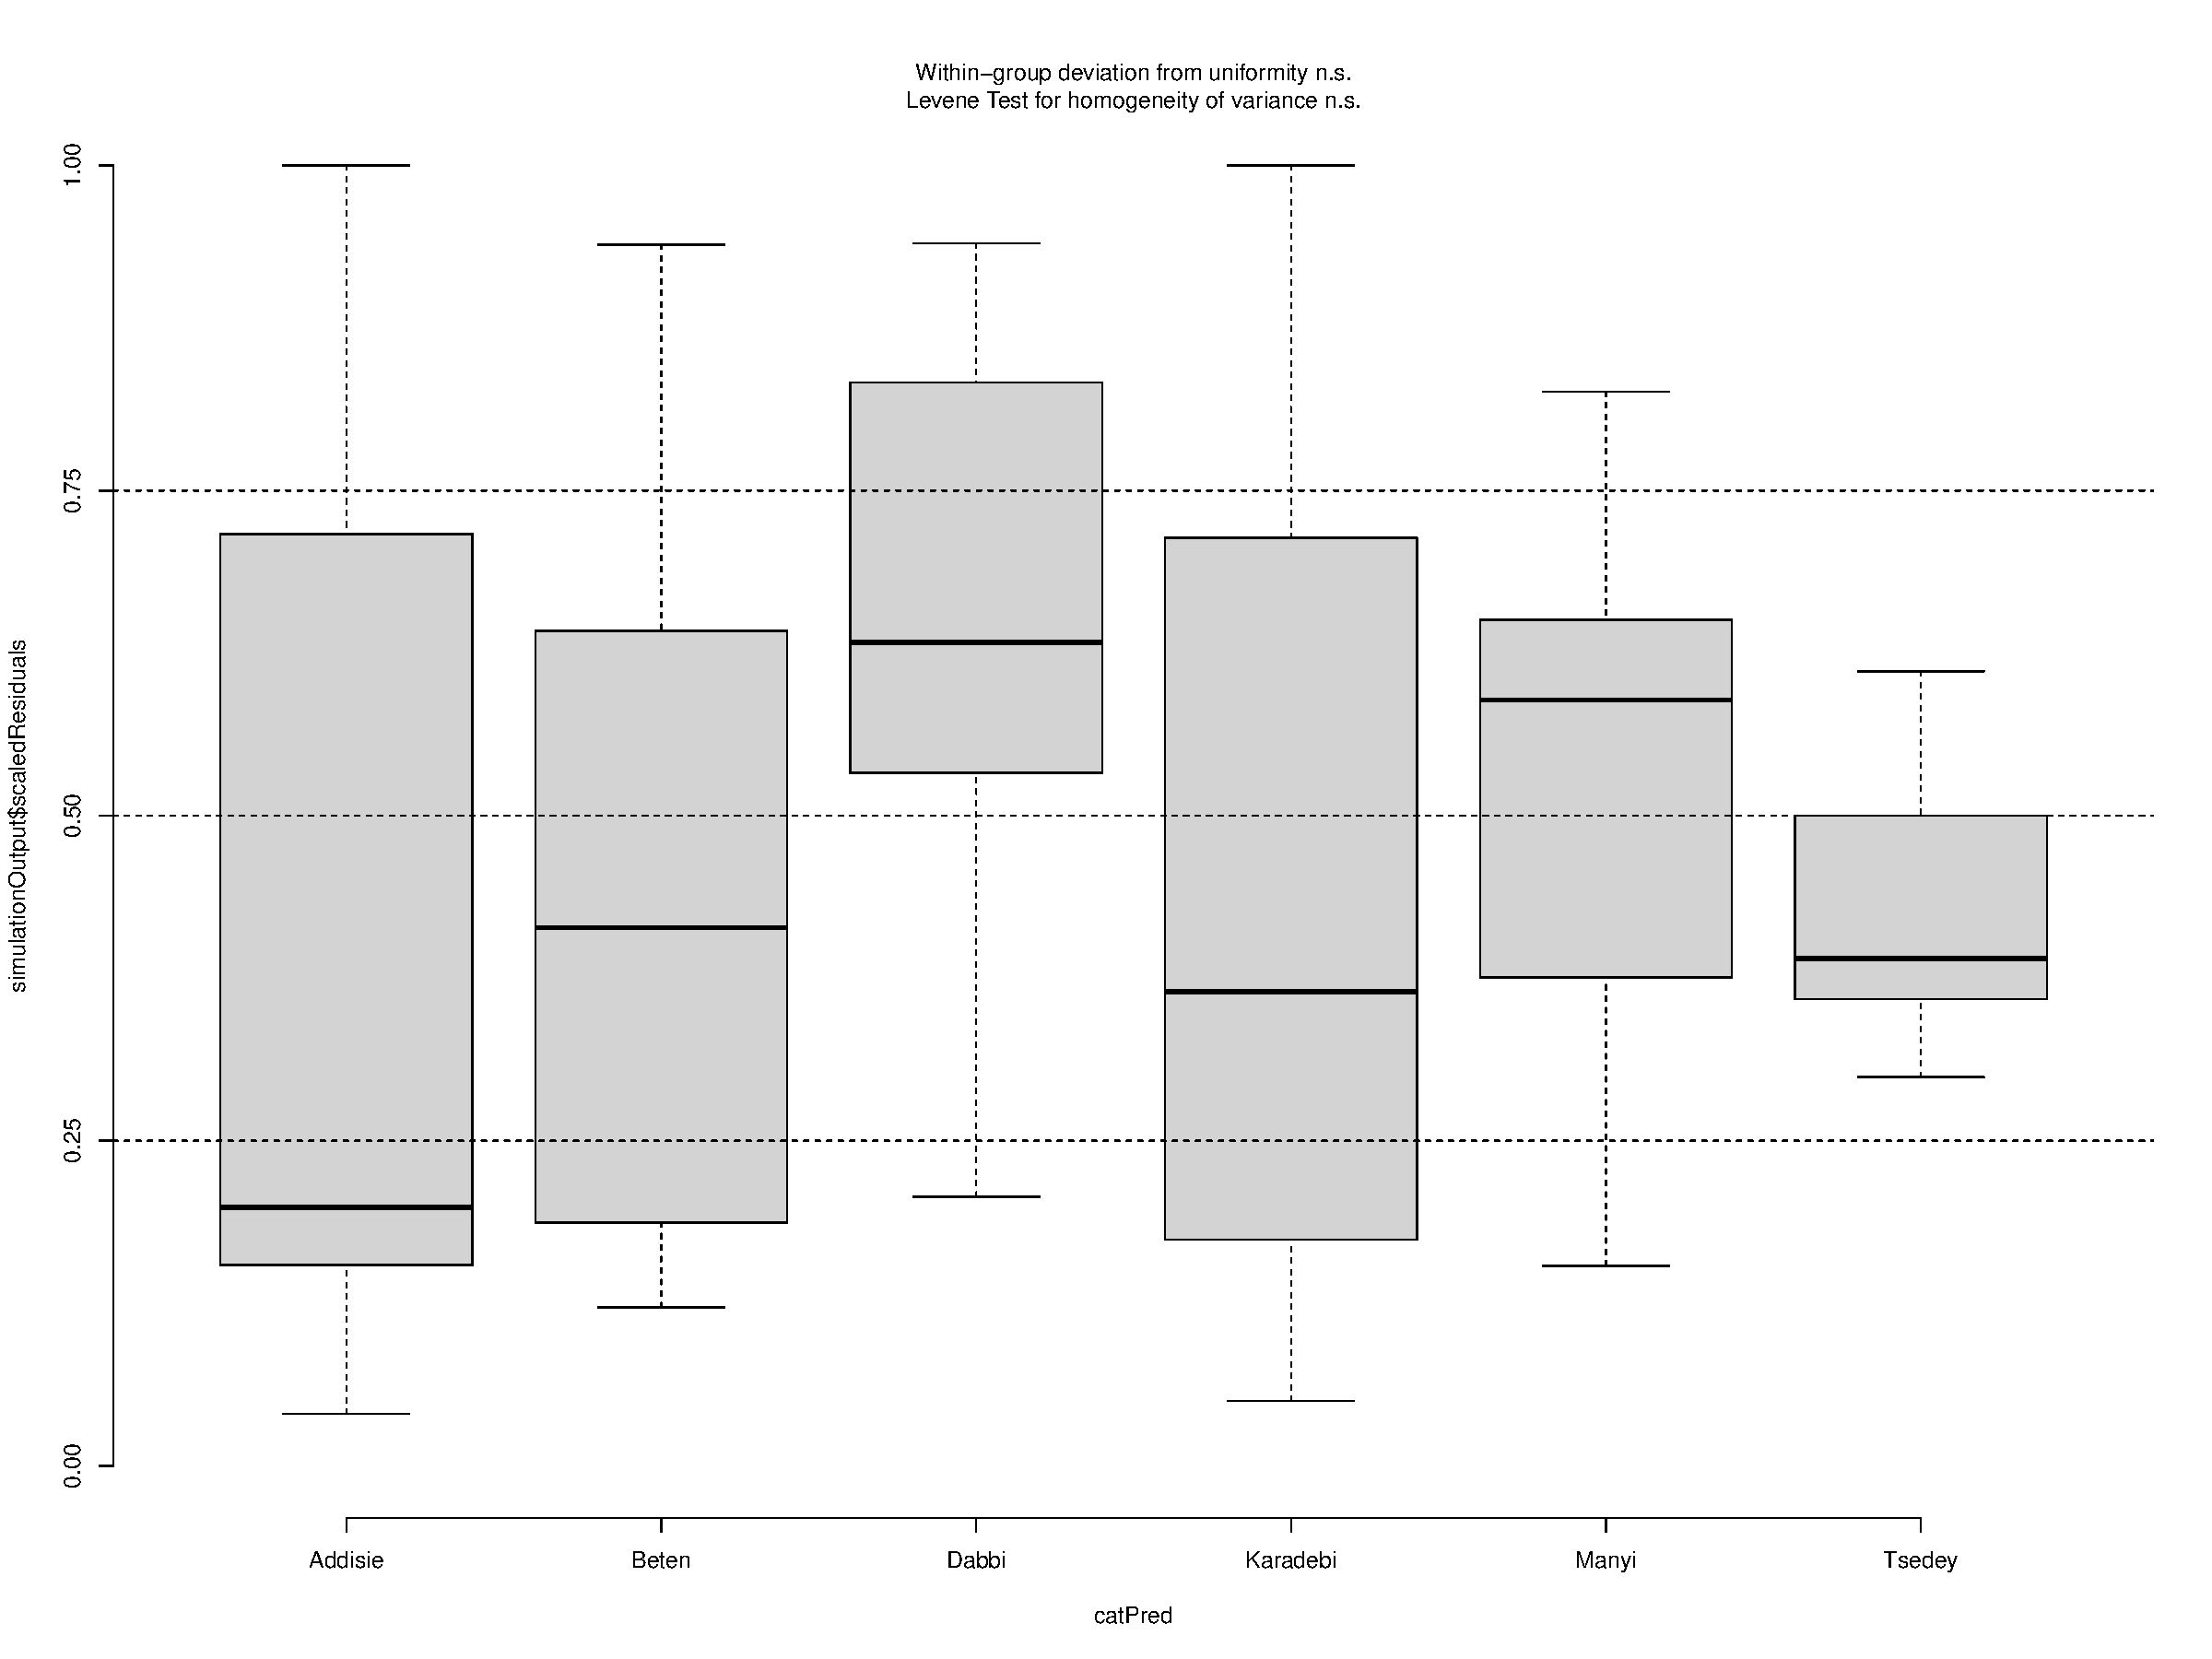
\includegraphics[keepaspectratio]{rsa_day1617_agar_files/figure-pdf/unnamed-chunk-6-5.pdf}}

\begin{Shaded}
\begin{Highlighting}[]
\CommentTok{\# residuals show poor fit (significant deviation from outlier test) so will log transform the data}

\CommentTok{\# ── 3. Log transformed model (use if full model fails) ─────────────}
\NormalTok{network\_tmb }\OtherTok{\textless{}{-}} \FunctionTok{glmmTMB}\NormalTok{(}
  \FunctionTok{log}\NormalTok{(Network.Area.mm2) }\SpecialCharTok{\textasciitilde{}}\NormalTok{ Genotype }\SpecialCharTok{+}\NormalTok{ (}\DecValTok{1} \SpecialCharTok{|}\NormalTok{ Batch) }\SpecialCharTok{+}\NormalTok{ (}\DecValTok{1} \SpecialCharTok{|}\NormalTok{ Seed}\SpecialCharTok{:}\NormalTok{Plate}\SpecialCharTok{:}\NormalTok{Batch),}
  \AttributeTok{data =}\NormalTok{ df, }\AttributeTok{family =} \FunctionTok{gaussian}\NormalTok{()}
\NormalTok{)}

\FunctionTok{VarCorr}\NormalTok{(network\_tmb)}
\end{Highlighting}
\end{Shaded}

\begin{verbatim}

Conditional model:
 Groups           Name        Std.Dev.
 Batch            (Intercept) 0.279262
 Seed:Plate:Batch (Intercept) 0.041489
 Residual                     0.406612
\end{verbatim}

\begin{Shaded}
\begin{Highlighting}[]
\FunctionTok{check\_singularity}\NormalTok{(network\_tmb)}
\end{Highlighting}
\end{Shaded}

\begin{verbatim}
[1] FALSE
\end{verbatim}

\begin{Shaded}
\begin{Highlighting}[]
\FunctionTok{summary}\NormalTok{(network\_tmb)   }\CommentTok{\# confirm real SEs and AIC}
\end{Highlighting}
\end{Shaded}

\begin{verbatim}
 Family: gaussian  ( identity )
Formula:          
log(Network.Area.mm2) ~ Genotype + (1 | Batch) + (1 | Seed:Plate:Batch)
Data: df

      AIC       BIC    logLik -2*log(L)  df.resid 
    101.3     121.6     -41.6      83.3        62 

Random effects:

Conditional model:
 Groups           Name        Variance Std.Dev.
 Batch            (Intercept) 0.077987 0.27926 
 Seed:Plate:Batch (Intercept) 0.001721 0.04149 
 Residual                     0.165334 0.40661 
Number of obs: 71, groups:  Batch, 4; Seed:Plate:Batch, 38

Dispersion estimate for gaussian family (sigma^2): 0.165 

Conditional model:
                 Estimate Std. Error z value Pr(>|z|)    
(Intercept)       3.34686    0.19317  17.326   <2e-16 ***
GenotypeBeten    -0.04745    0.16736  -0.284   0.7768    
GenotypeDabbi    -0.04575    0.19087  -0.240   0.8106    
GenotypeKaradebi -0.06614    0.18988  -0.348   0.7276    
GenotypeManyi     0.13510    0.22475   0.601   0.5478    
GenotypeTsedey   -0.35273    0.18237  -1.934   0.0531 .  
---
Signif. codes:  0 '***' 0.001 '**' 0.01 '*' 0.05 '.' 0.1 ' ' 1
\end{verbatim}

\begin{Shaded}
\begin{Highlighting}[]
\CommentTok{\# ── 4. Assumption checks ──────────────────────────────────────}
\NormalTok{sim\_res }\OtherTok{\textless{}{-}} \FunctionTok{simulateResiduals}\NormalTok{(network\_tmb, }\AttributeTok{n =} \DecValTok{1000}\NormalTok{)}
\FunctionTok{plot}\NormalTok{(sim\_res)}
\end{Highlighting}
\end{Shaded}

\pandocbounded{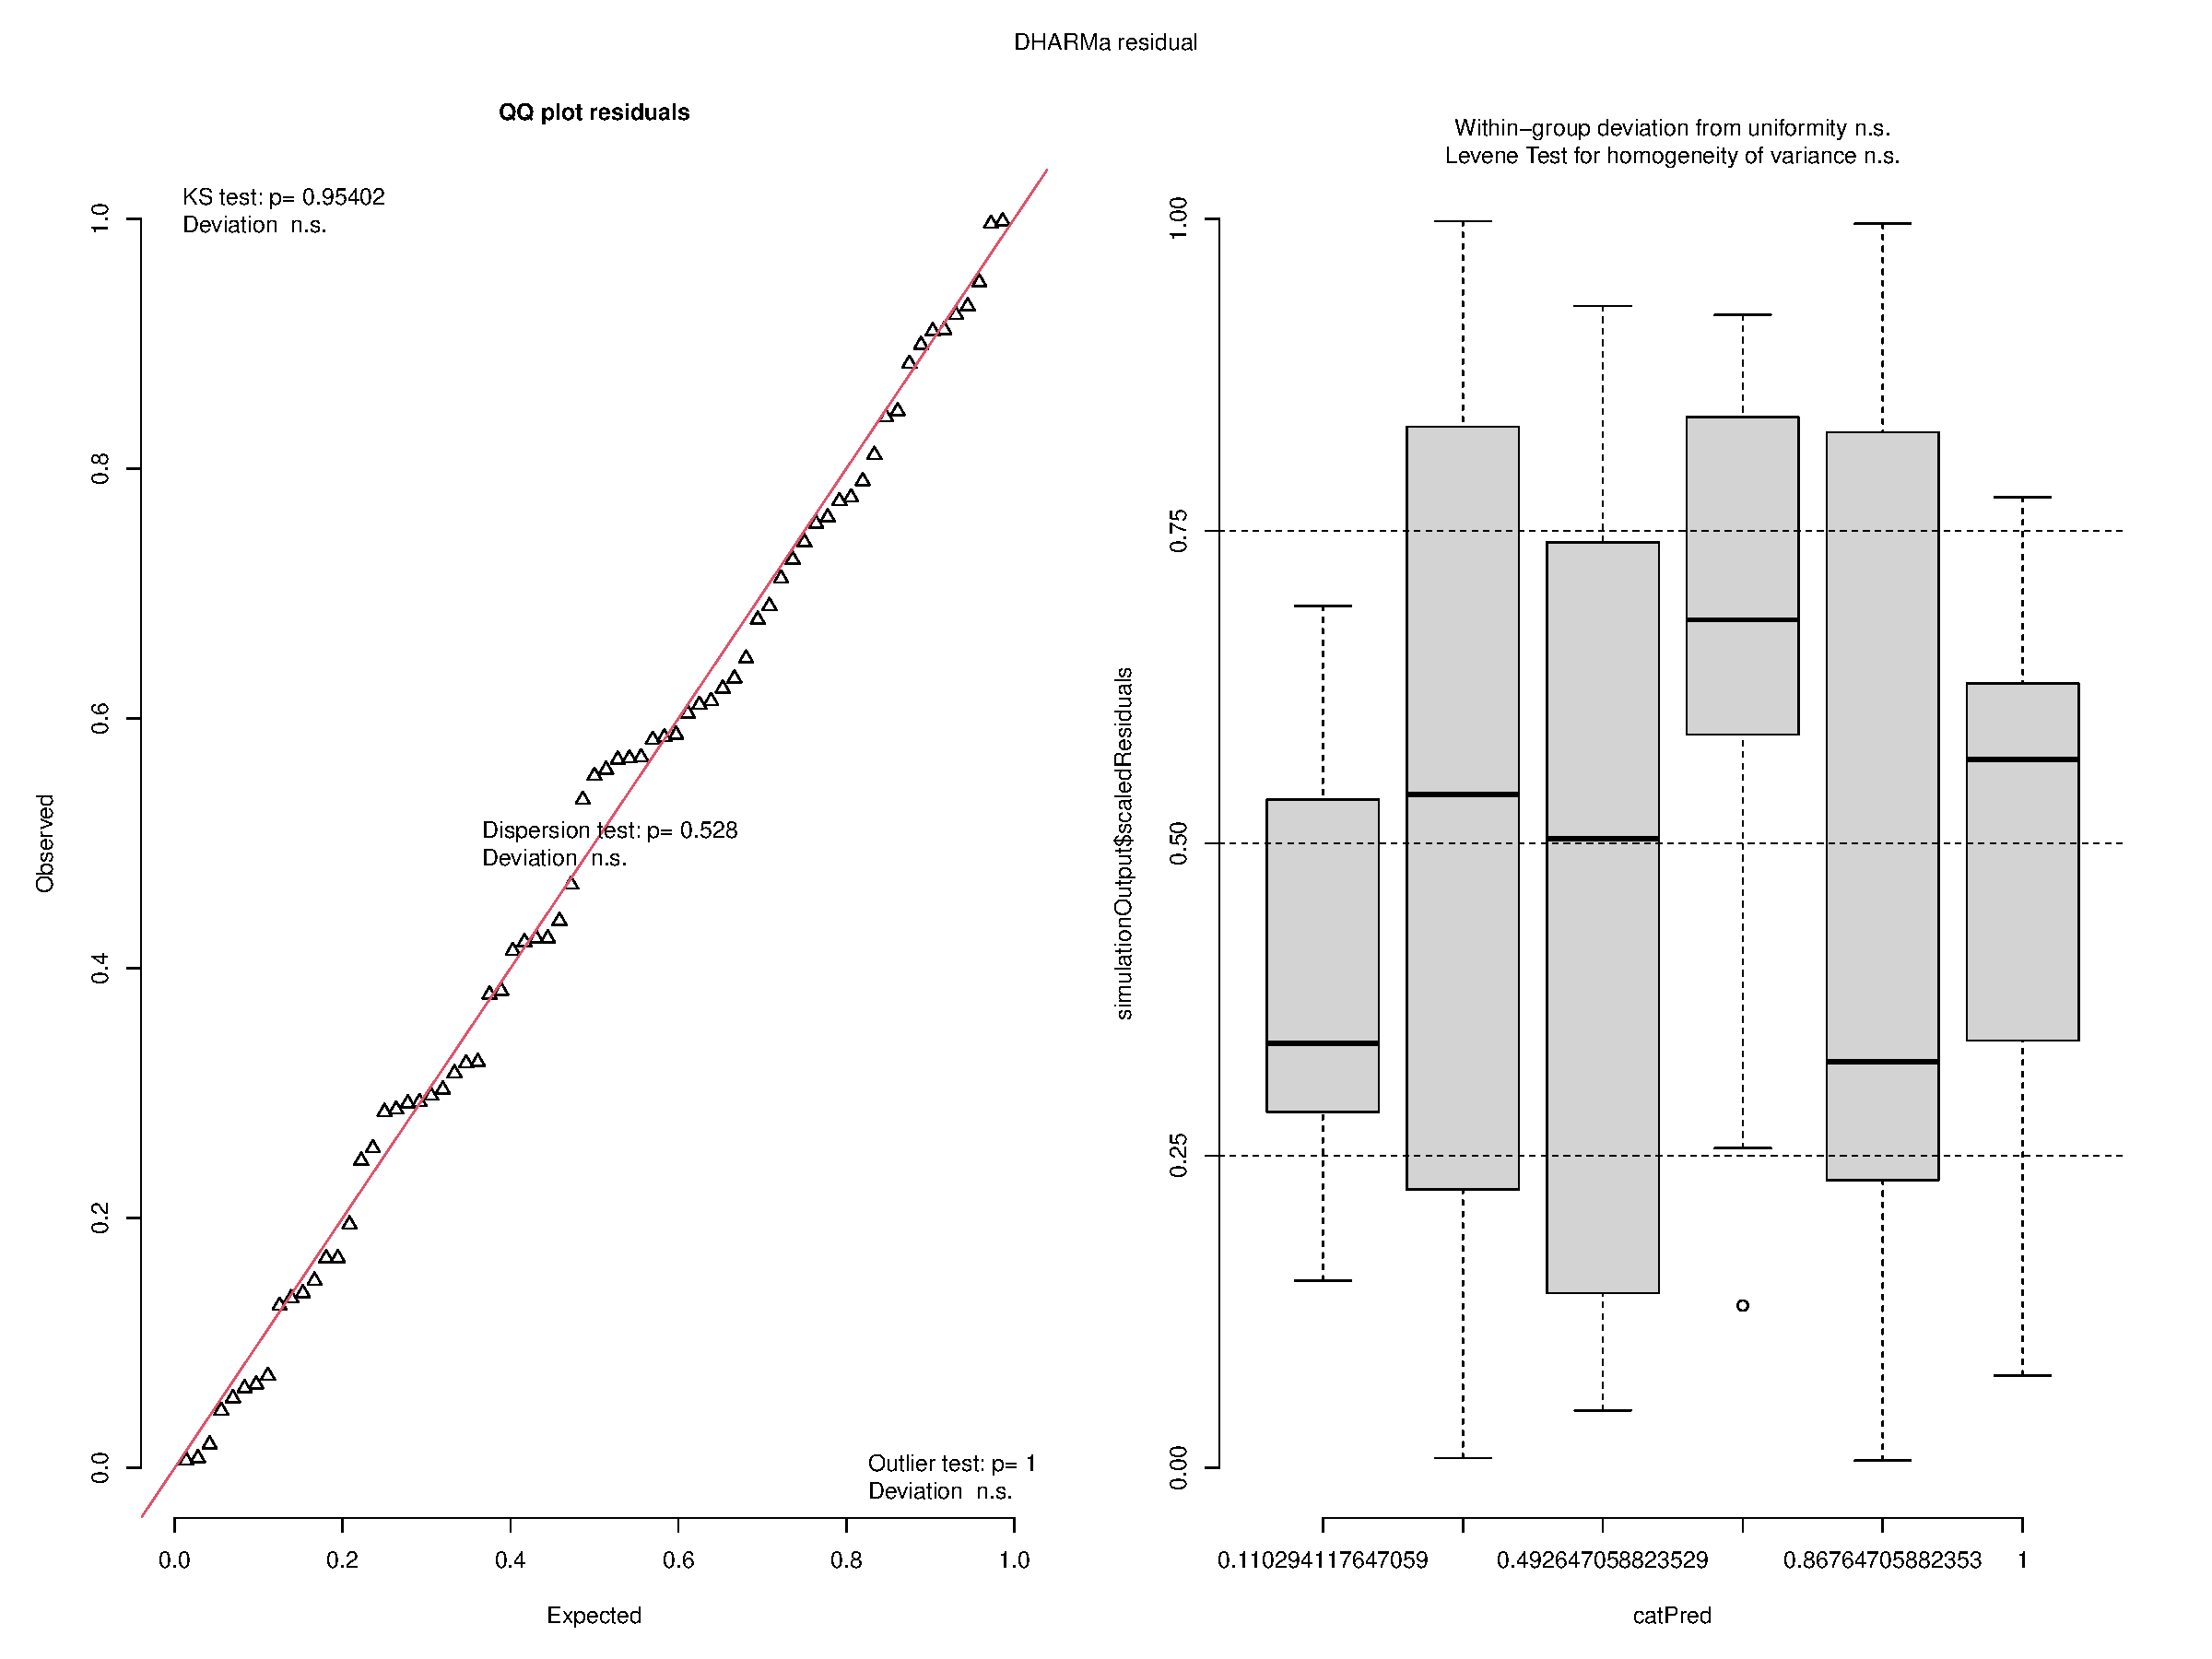
\includegraphics[keepaspectratio]{rsa_day1617_agar_files/figure-pdf/unnamed-chunk-6-6.pdf}}

\begin{Shaded}
\begin{Highlighting}[]
\FunctionTok{testUniformity}\NormalTok{(sim\_res)}
\end{Highlighting}
\end{Shaded}

\pandocbounded{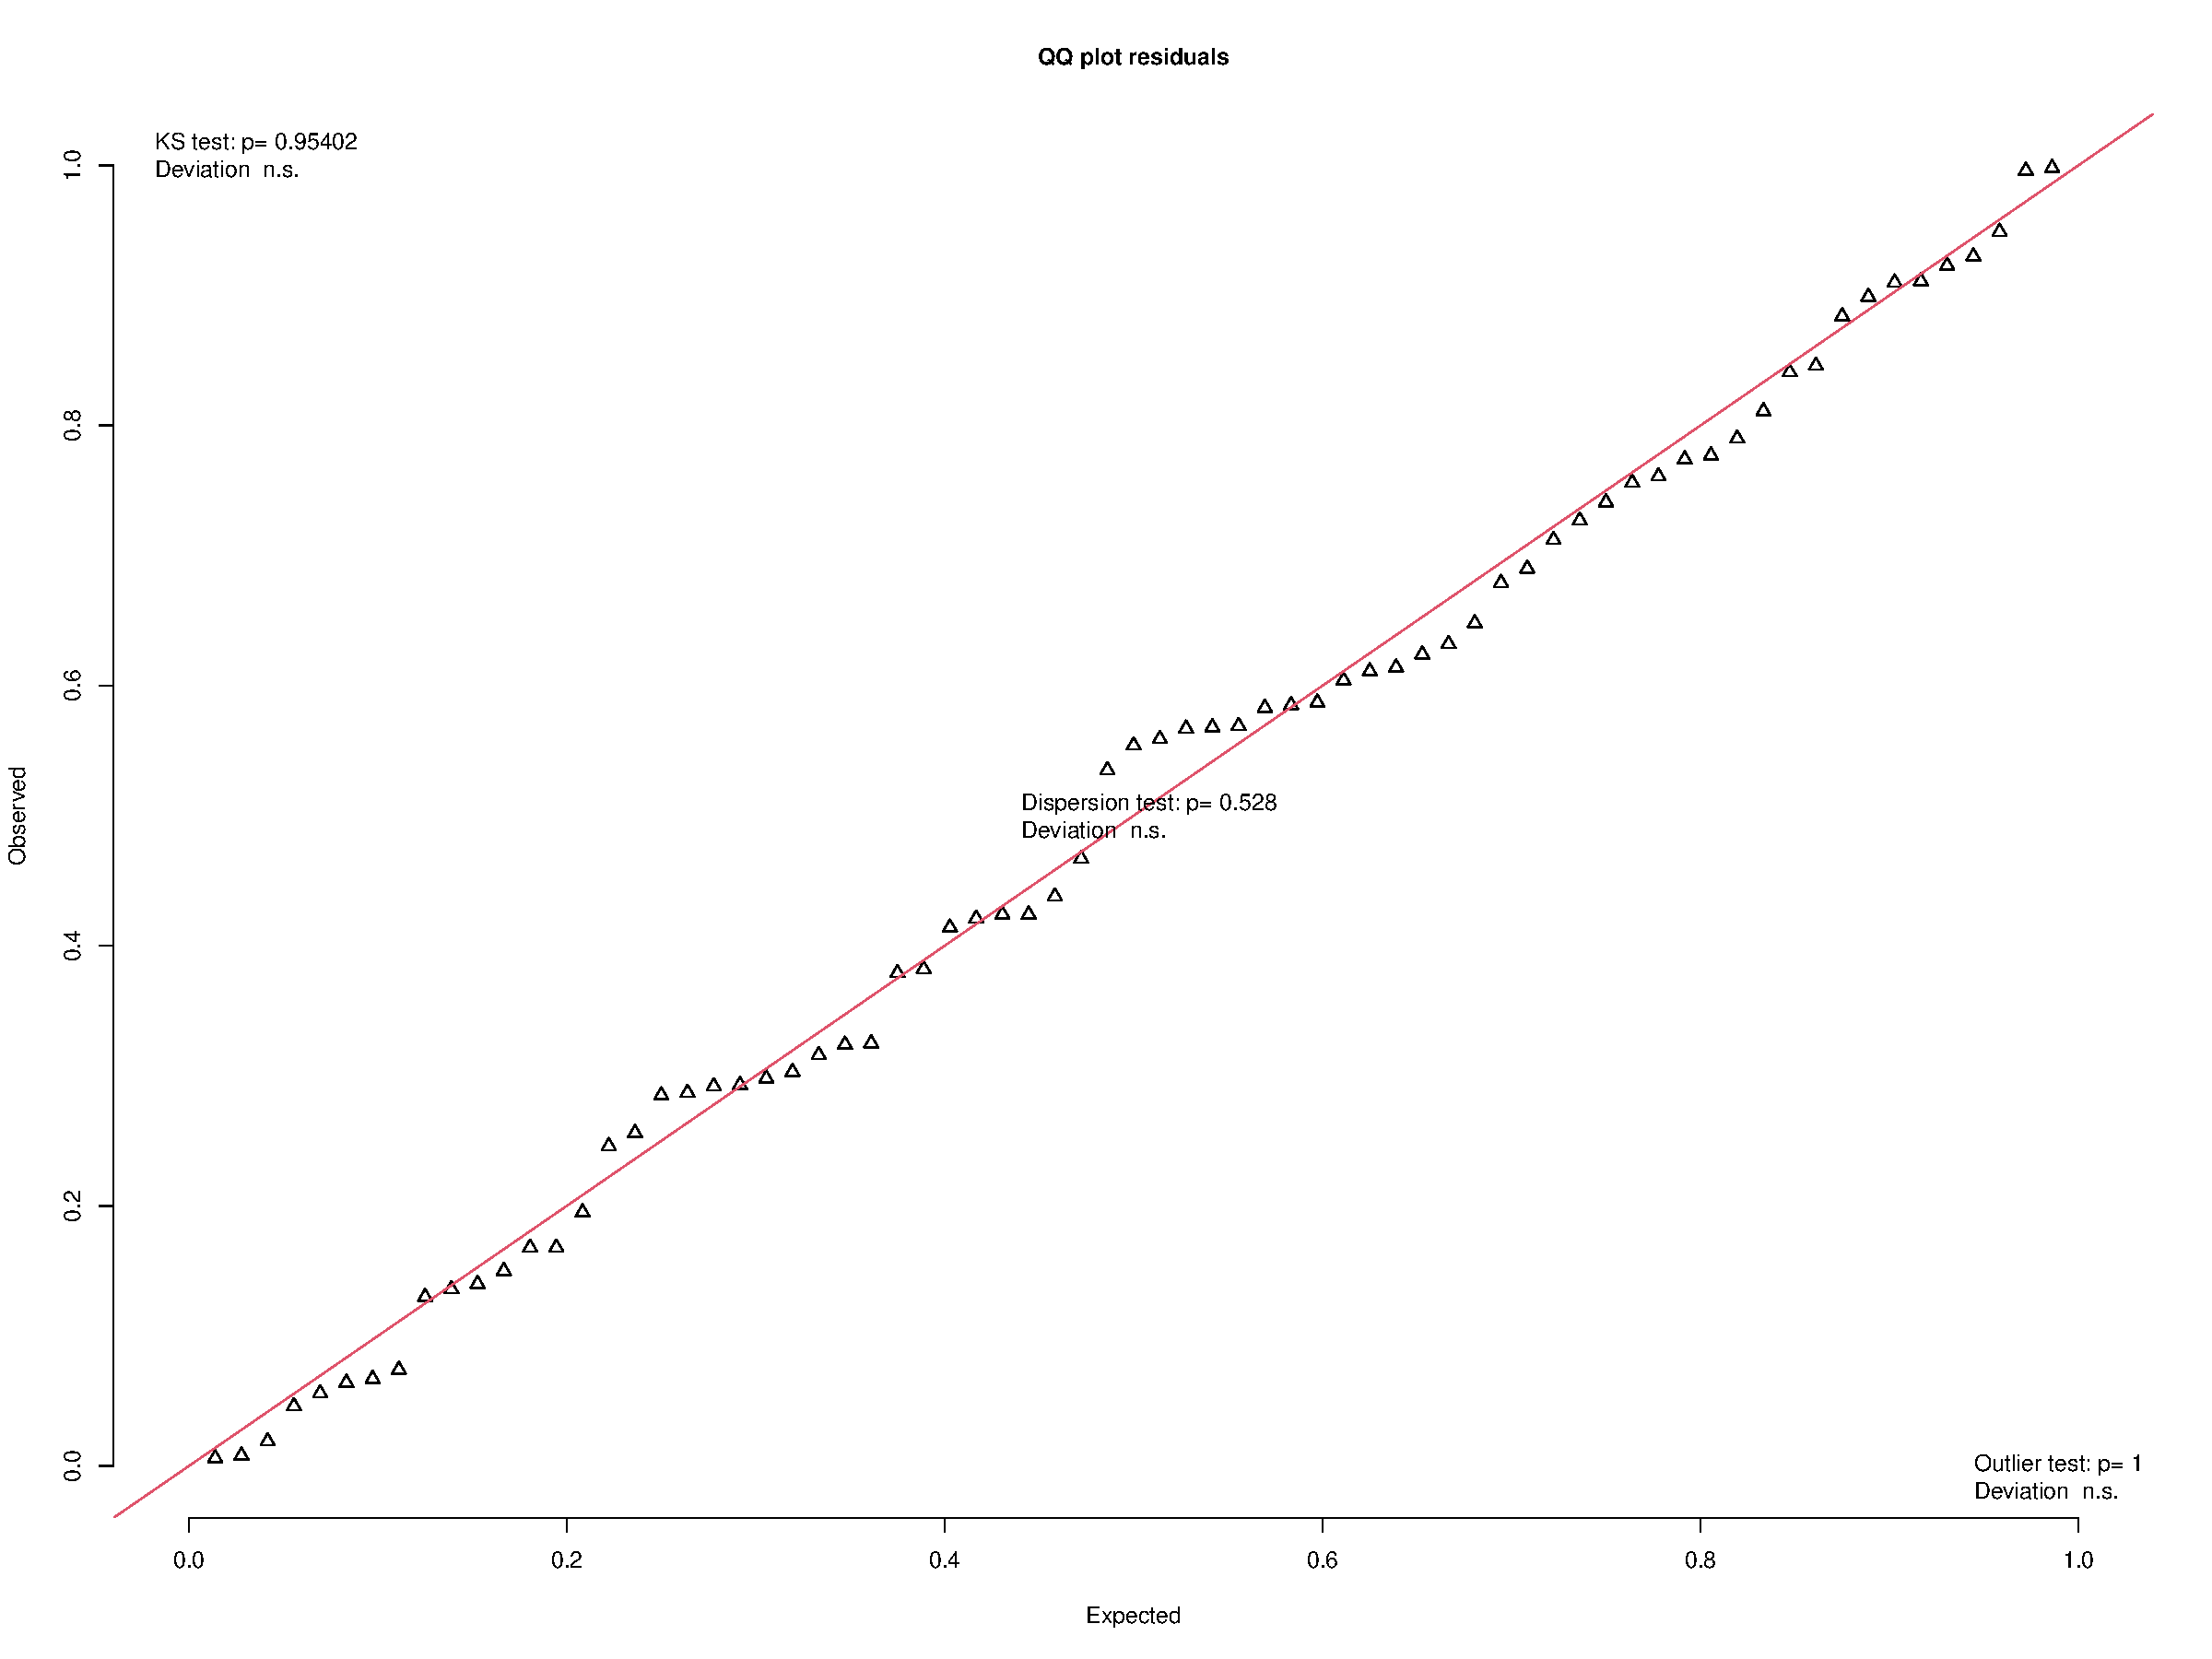
\includegraphics[keepaspectratio]{rsa_day1617_agar_files/figure-pdf/unnamed-chunk-6-7.pdf}}

\begin{verbatim}

    Asymptotic one-sample Kolmogorov-Smirnov test

data:  simulationOutput$scaledResiduals
D = 0.061042, p-value = 0.954
alternative hypothesis: two-sided
\end{verbatim}

\begin{Shaded}
\begin{Highlighting}[]
\FunctionTok{testDispersion}\NormalTok{(sim\_res)}
\end{Highlighting}
\end{Shaded}

\pandocbounded{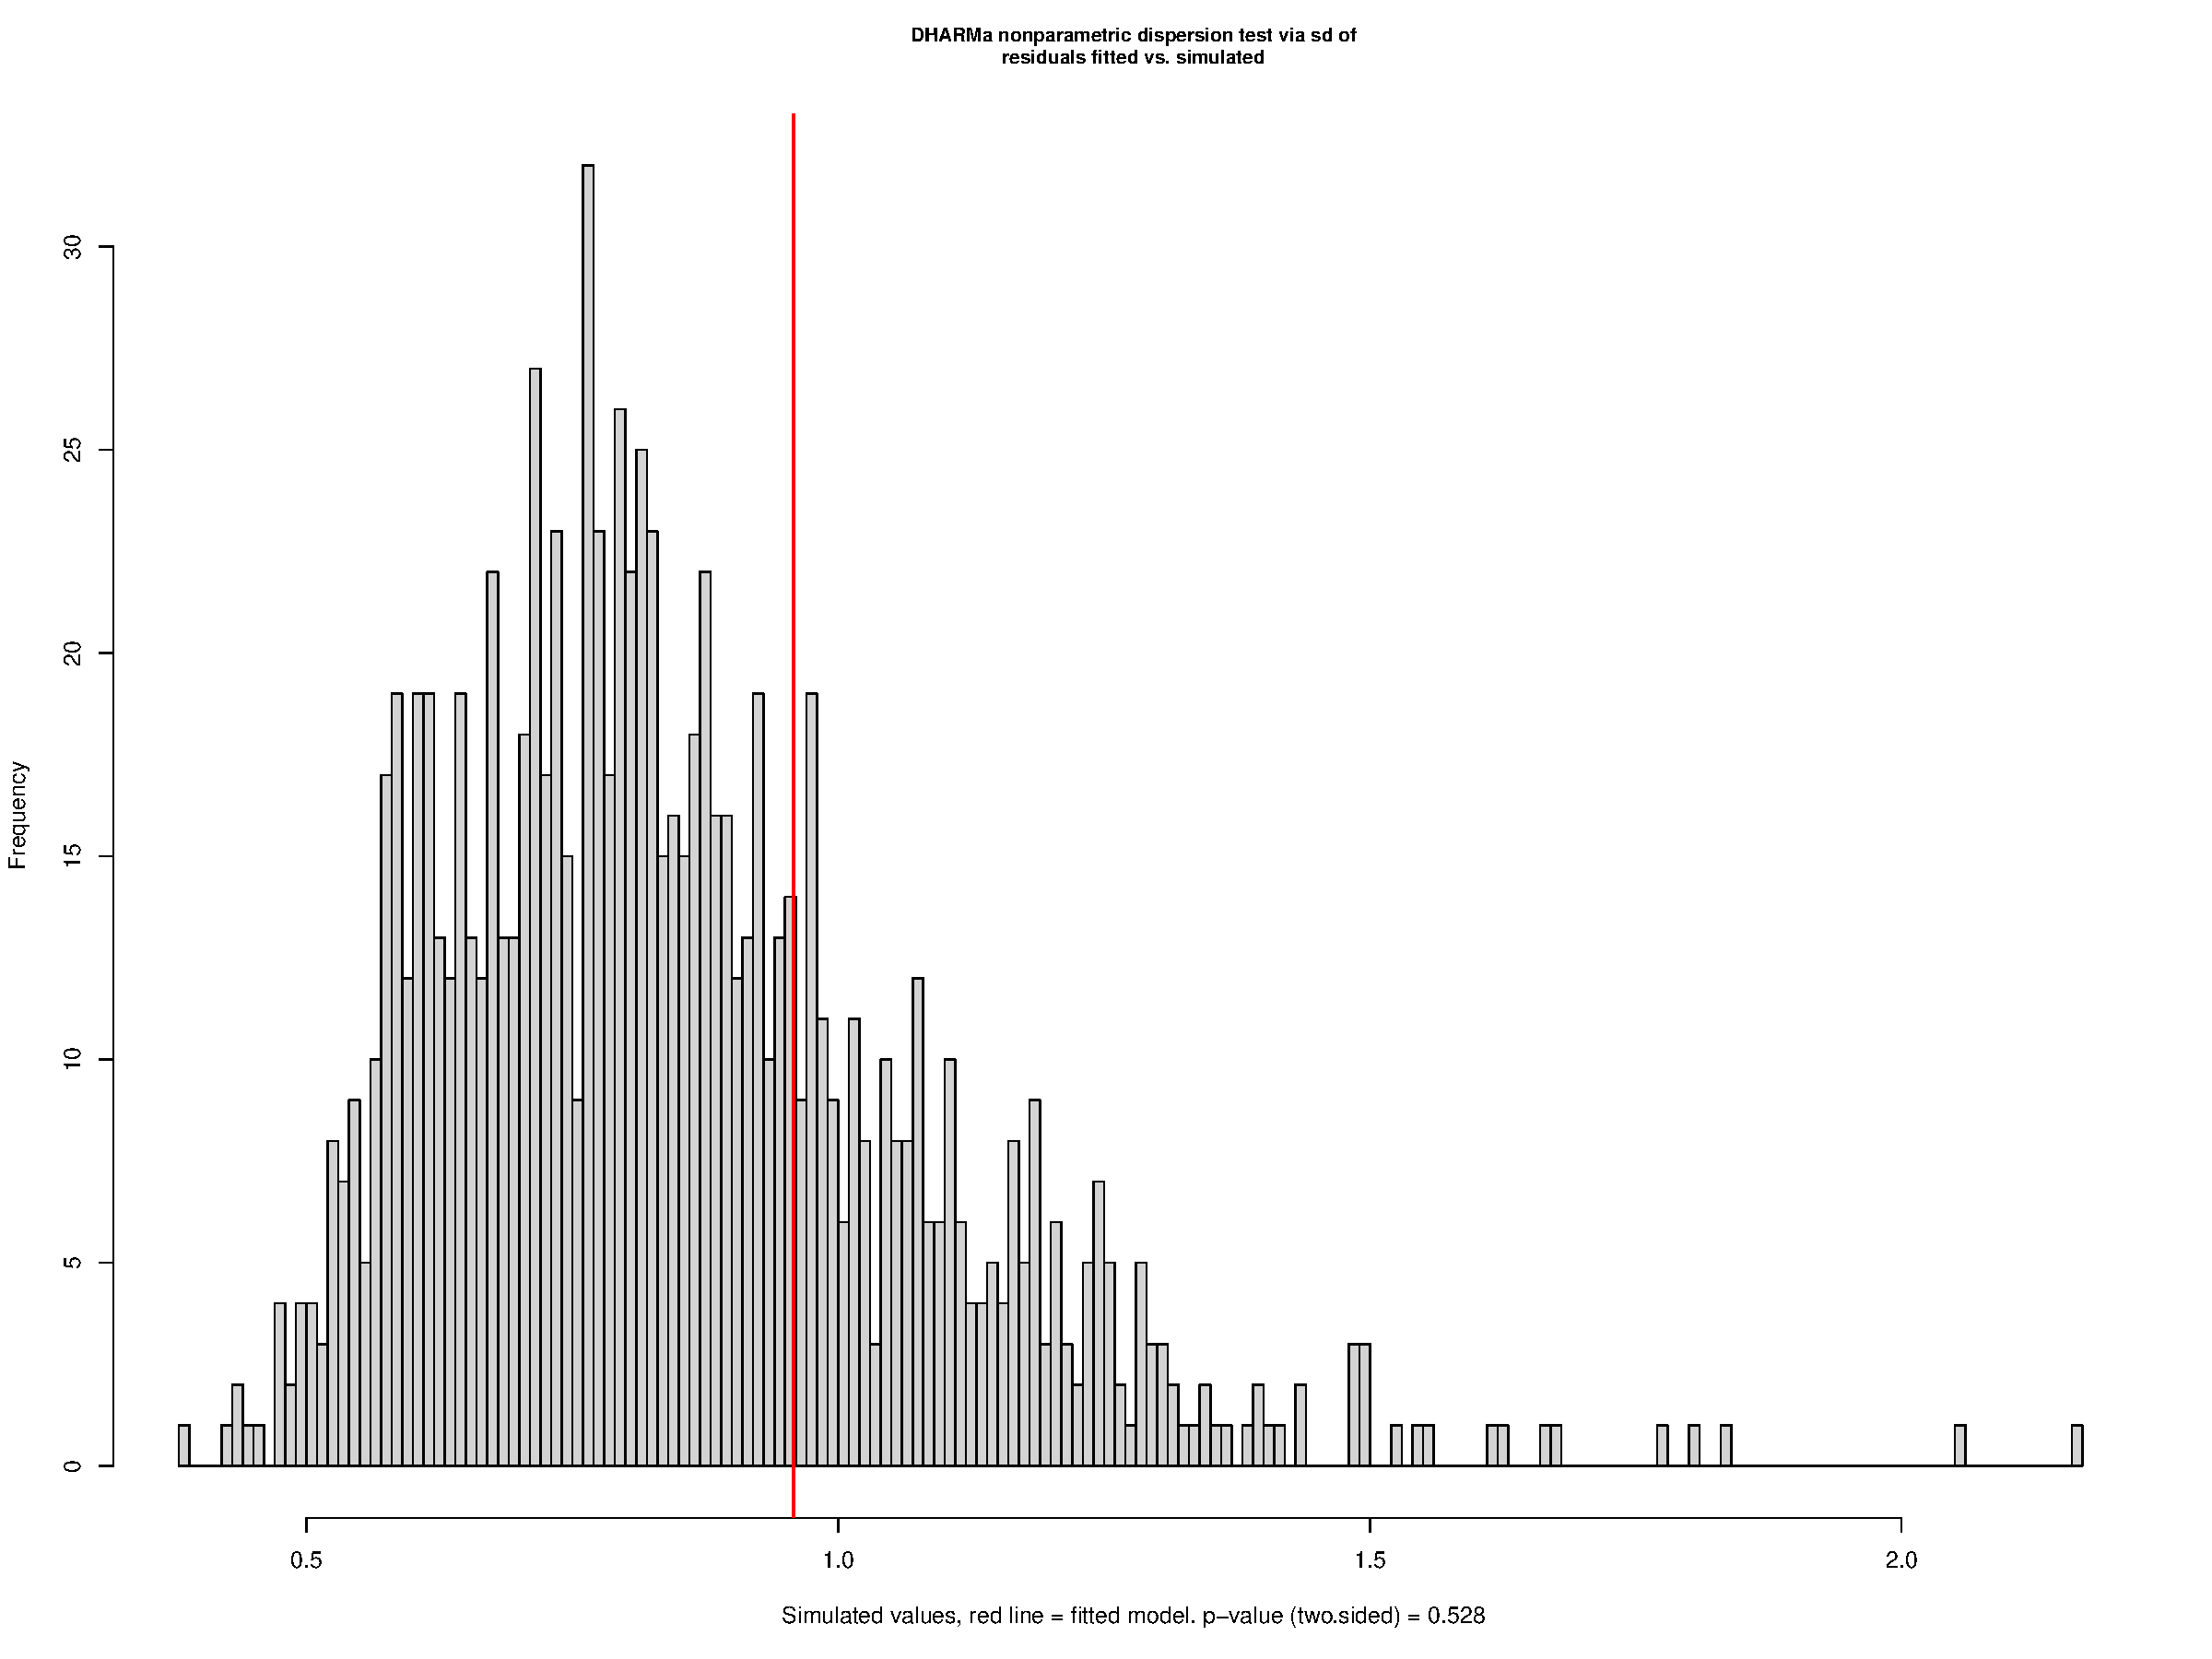
\includegraphics[keepaspectratio]{rsa_day1617_agar_files/figure-pdf/unnamed-chunk-6-8.pdf}}

\begin{verbatim}

    DHARMa nonparametric dispersion test via sd of residuals fitted vs.
    simulated

data:  simulationOutput
dispersion = 1.1276, p-value = 0.528
alternative hypothesis: two.sided
\end{verbatim}

\begin{Shaded}
\begin{Highlighting}[]
\FunctionTok{plotResiduals}\NormalTok{(sim\_res, }\AttributeTok{form =}\NormalTok{ df}\SpecialCharTok{$}\NormalTok{Genotype)}
\end{Highlighting}
\end{Shaded}

\pandocbounded{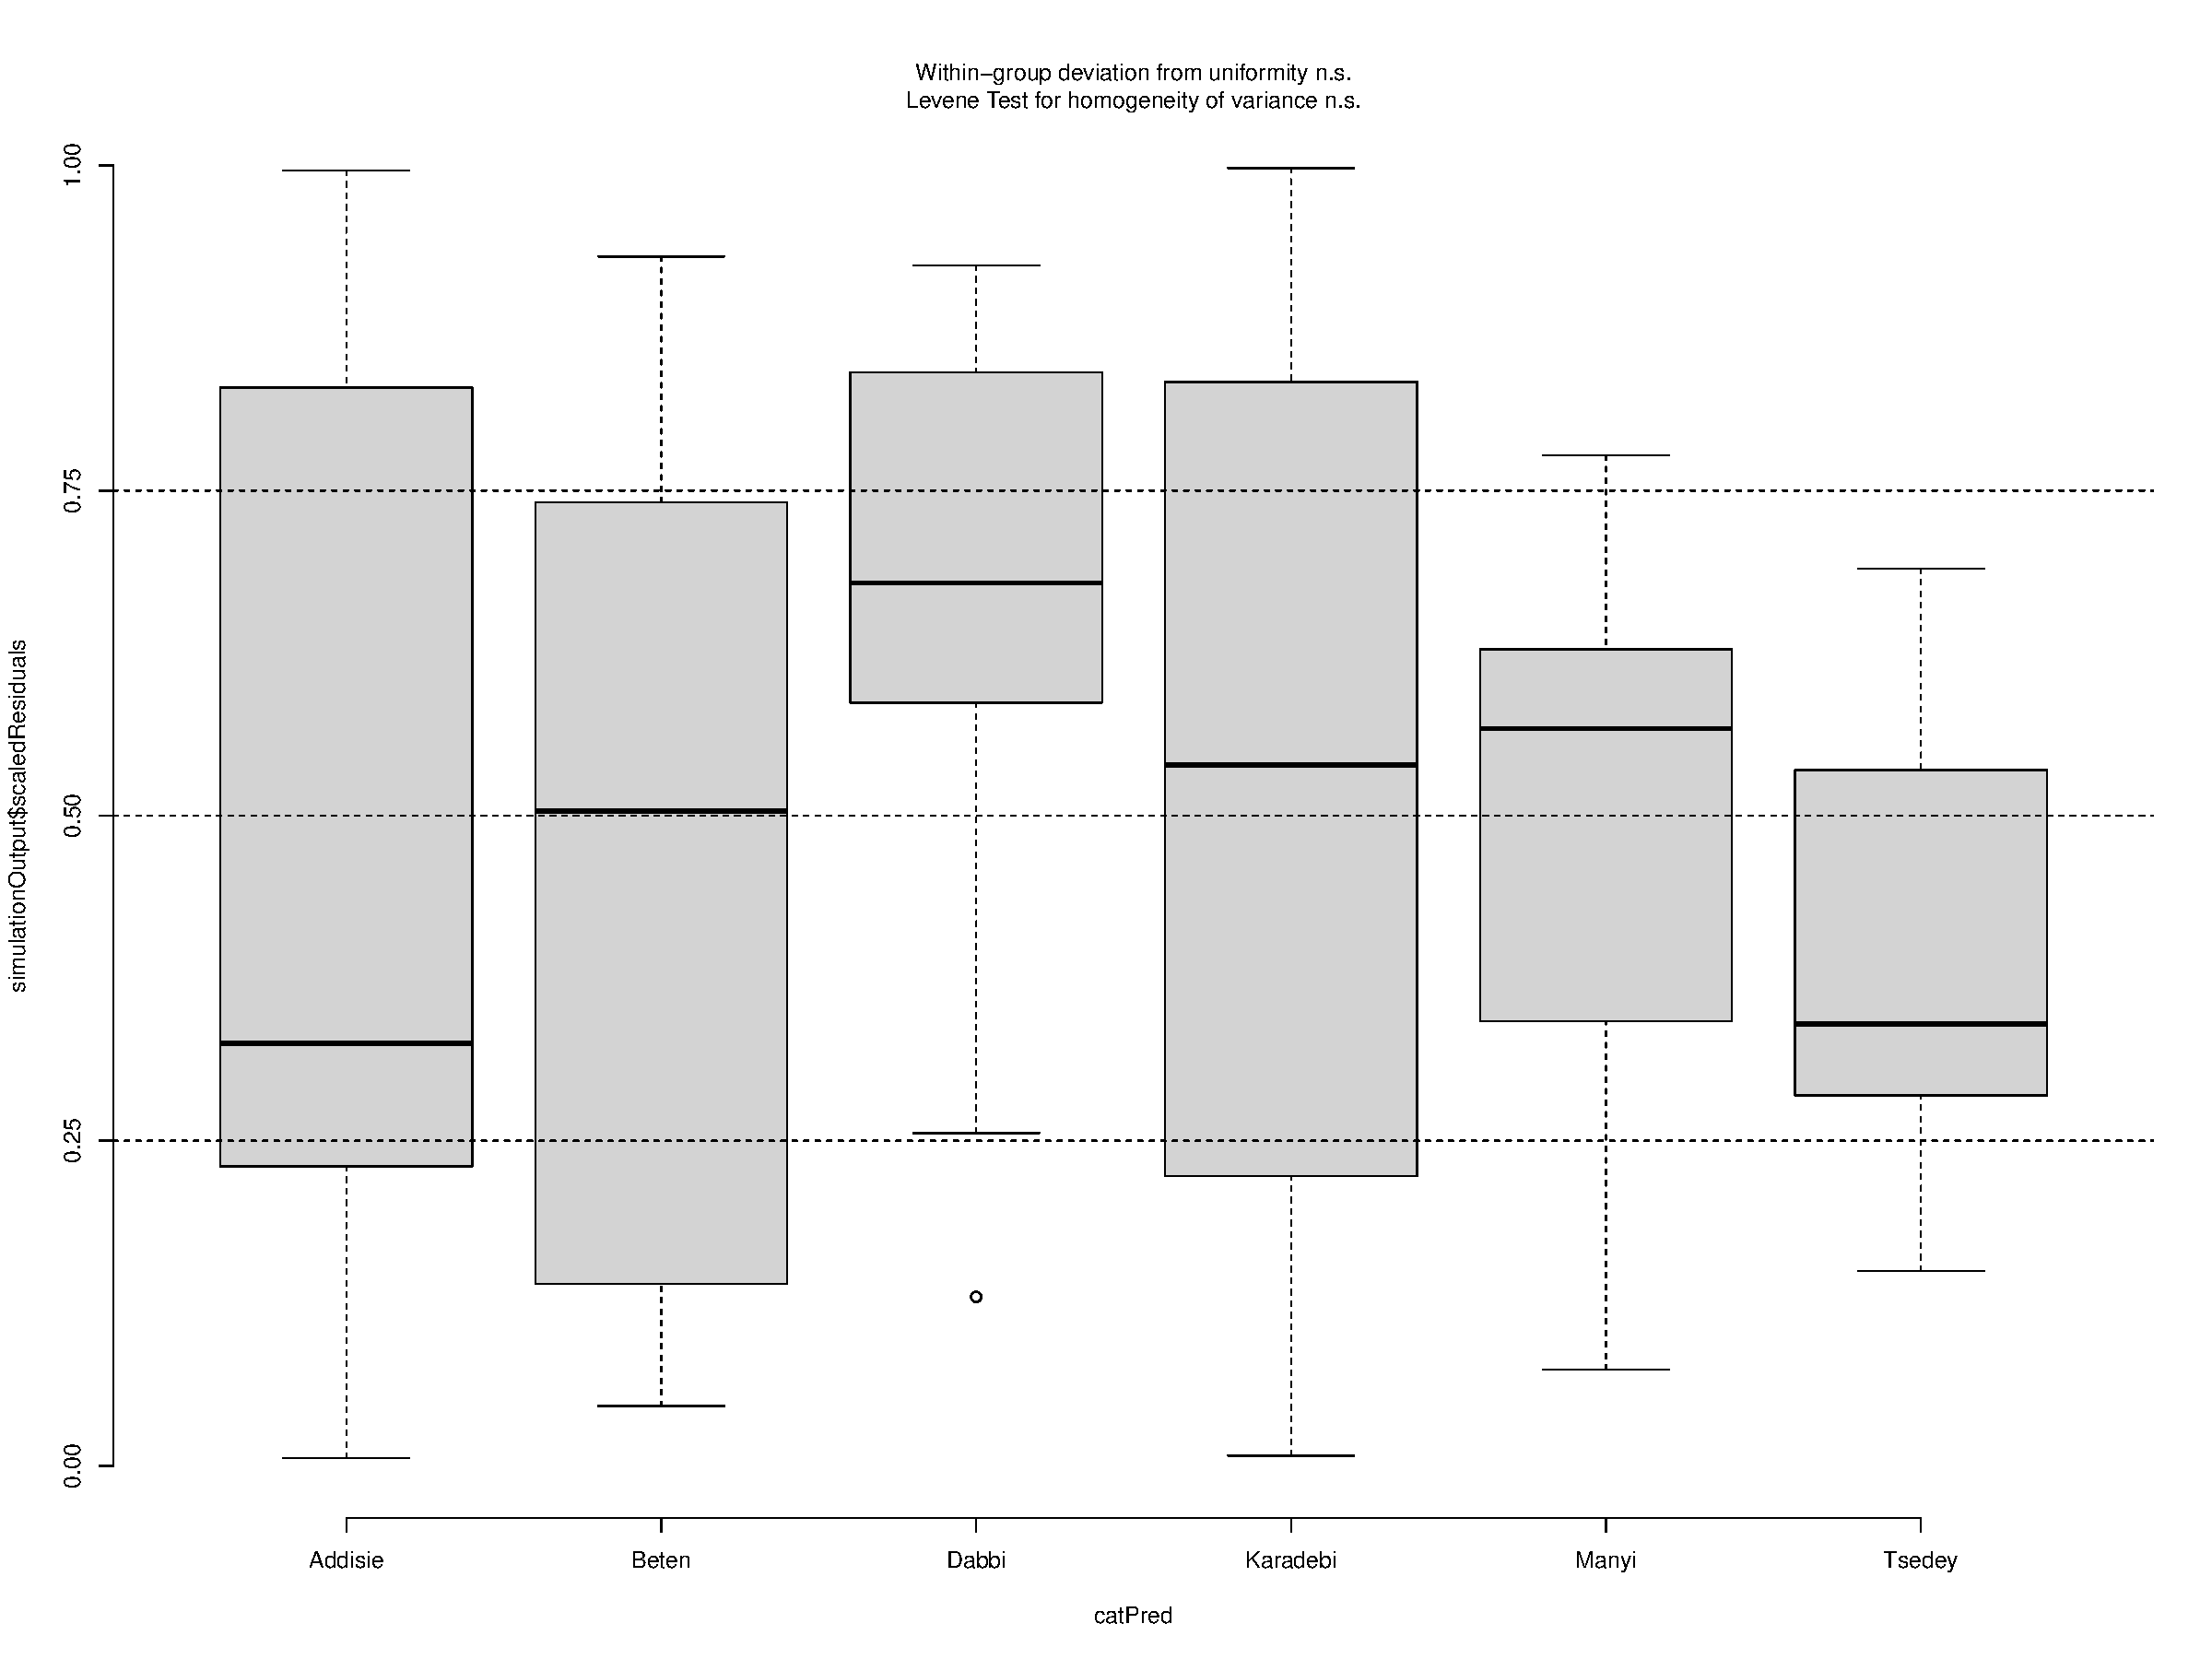
\includegraphics[keepaspectratio]{rsa_day1617_agar_files/figure-pdf/unnamed-chunk-6-9.pdf}}

\begin{Shaded}
\begin{Highlighting}[]
\CommentTok{\# ── 5. Test overall Genotype effect ──────────────────────────}
\NormalTok{car}\SpecialCharTok{::}\FunctionTok{Anova}\NormalTok{(network\_tmb, }\AttributeTok{type =} \StringTok{"III"}\NormalTok{)}
\end{Highlighting}
\end{Shaded}

\begin{verbatim}
Analysis of Deviance Table (Type III Wald chisquare tests)

Response: log(Network.Area.mm2)
               Chisq Df Pr(>Chisq)    
(Intercept) 300.1782  1     <2e-16 ***
Genotype      7.7516  5     0.1705    
---
Signif. codes:  0 '***' 0.001 '**' 0.01 '*' 0.05 '.' 0.1 ' ' 1
\end{verbatim}

\begin{Shaded}
\begin{Highlighting}[]
\CommentTok{\# ── 6. Pairwise comparisons + CLD ────────────────────────────}
\NormalTok{emm }\OtherTok{\textless{}{-}} \FunctionTok{emmeans}\NormalTok{(network\_tmb, }\SpecialCharTok{\textasciitilde{}}\NormalTok{ Genotype, }\AttributeTok{type =} \StringTok{"response"}\NormalTok{)}
\FunctionTok{pairs}\NormalTok{(emm, }\AttributeTok{adjust =} \StringTok{"sidak"}\NormalTok{)}
\end{Highlighting}
\end{Shaded}

\begin{verbatim}
 contrast           ratio    SE  df null z.ratio p.value
 Addisie / Beten    1.049 0.175 Inf    1   0.284  1.0000
 Addisie / Dabbi    1.047 0.200 Inf    1   0.240  1.0000
 Addisie / Karadebi 1.068 0.203 Inf    1   0.348  1.0000
 Addisie / Manyi    0.874 0.196 Inf    1  -0.601  1.0000
 Addisie / Tsedey   1.423 0.260 Inf    1   1.934  0.5588
 Beten / Dabbi      0.998 0.185 Inf    1  -0.009  1.0000
 Beten / Karadebi   1.019 0.181 Inf    1   0.105  1.0000
 Beten / Manyi      0.833 0.175 Inf    1  -0.867  0.9993
 Beten / Tsedey     1.357 0.224 Inf    1   1.849  0.6317
 Dabbi / Karadebi   1.021 0.176 Inf    1   0.119  1.0000
 Dabbi / Manyi      0.835 0.170 Inf    1  -0.888  0.9991
 Dabbi / Tsedey     1.359 0.256 Inf    1   1.630  0.8045
 Karadebi / Manyi   0.818 0.164 Inf    1  -1.006  0.9965
 Karadebi / Tsedey  1.332 0.242 Inf    1   1.578  0.8386
 Manyi / Tsedey     1.629 0.326 Inf    1   2.436  0.2010

P value adjustment: sidak method for 15 tests 
Tests are performed on the log scale 
\end{verbatim}

\begin{Shaded}
\begin{Highlighting}[]
\NormalTok{cld\_df }\OtherTok{\textless{}{-}} \FunctionTok{as.data.frame}\NormalTok{(}\FunctionTok{cld}\NormalTok{(emm, }\AttributeTok{adjust =} \StringTok{"sidak"}\NormalTok{,}
                             \AttributeTok{Letters =}\NormalTok{ letters, }\AttributeTok{alpha =} \FloatTok{0.05}\NormalTok{)) }\SpecialCharTok{\%\textgreater{}\%}
  \FunctionTok{mutate}\NormalTok{(}\AttributeTok{.group =} \FunctionTok{trimws}\NormalTok{(.group))}

\NormalTok{n\_df }\OtherTok{\textless{}{-}}\NormalTok{ df }\SpecialCharTok{\%\textgreater{}\%}
  \FunctionTok{count}\NormalTok{(Genotype) }\SpecialCharTok{\%\textgreater{}\%}
  \FunctionTok{mutate}\NormalTok{(}\AttributeTok{label =} \FunctionTok{paste0}\NormalTok{(}\StringTok{"n="}\NormalTok{, n))}


\CommentTok{\# ── 7. Plot 1 — Boxplot ───────────────────────────────────────}

\NormalTok{y\_ceil }\OtherTok{\textless{}{-}} \FunctionTok{max}\NormalTok{(df}\SpecialCharTok{$}\NormalTok{Network.Area.mm2) }\SpecialCharTok{*} \FloatTok{1.22}
\NormalTok{y\_label }\OtherTok{\textless{}{-}}\NormalTok{ y\_ceil }\SpecialCharTok{*} \FloatTok{0.8555}

\NormalTok{p1 }\OtherTok{\textless{}{-}} \FunctionTok{ggplot}\NormalTok{(df, }\FunctionTok{aes}\NormalTok{(}\AttributeTok{x =}\NormalTok{ Genotype, }\AttributeTok{y =}\NormalTok{ Network.Area.mm2, }\AttributeTok{fill =}\NormalTok{ Genotype)) }\SpecialCharTok{+}

  \FunctionTok{geom\_boxplot}\NormalTok{(}
    \AttributeTok{alpha =} \FloatTok{0.7}\NormalTok{, }\AttributeTok{outlier.shape =} \ConstantTok{NA}\NormalTok{,}
    \AttributeTok{width =} \FloatTok{0.5}\NormalTok{, }\AttributeTok{colour =} \StringTok{"black"}\NormalTok{, }\AttributeTok{linewidth =} \FloatTok{0.5}
\NormalTok{  ) }\SpecialCharTok{+}

  \FunctionTok{geom\_jitter}\NormalTok{(}\AttributeTok{width =} \FloatTok{0.15}\NormalTok{, }\AttributeTok{size =} \FloatTok{1.8}\NormalTok{, }\AttributeTok{alpha =} \FloatTok{0.55}\NormalTok{, }\AttributeTok{colour =} \StringTok{"black"}\NormalTok{) }\SpecialCharTok{+}

  \FunctionTok{geom\_text}\NormalTok{(}
    \AttributeTok{data =}\NormalTok{ cld\_df, }\FunctionTok{aes}\NormalTok{(}\AttributeTok{x =}\NormalTok{ Genotype, }\AttributeTok{label =}\NormalTok{ .group),}
    \AttributeTok{y =}\NormalTok{ y\_label, }\AttributeTok{inherit.aes =} \ConstantTok{FALSE}\NormalTok{,}
    \AttributeTok{size =} \DecValTok{5}\NormalTok{, }\AttributeTok{fontface =} \StringTok{"bold"}\NormalTok{, }\AttributeTok{colour =} \StringTok{"grey20"}
\NormalTok{  ) }\SpecialCharTok{+}

  \FunctionTok{geom\_text}\NormalTok{(}
    \AttributeTok{data =}\NormalTok{ n\_df, }\FunctionTok{aes}\NormalTok{(}\AttributeTok{x =}\NormalTok{ Genotype, }\AttributeTok{label =}\NormalTok{ label),}
    \AttributeTok{y =} \SpecialCharTok{{-}}\ConstantTok{Inf}\NormalTok{, }\AttributeTok{vjust =} \FloatTok{4.2}\NormalTok{, }\AttributeTok{inherit.aes =} \ConstantTok{FALSE}\NormalTok{,}
    \AttributeTok{size =} \FloatTok{3.5}\NormalTok{, }\AttributeTok{colour =} \StringTok{"grey40"}
\NormalTok{  ) }\SpecialCharTok{+}

  \FunctionTok{scale\_fill\_brewer}\NormalTok{(}\AttributeTok{palette =} \StringTok{"Set2"}\NormalTok{) }\SpecialCharTok{+}
 
  \FunctionTok{labs}\NormalTok{(}
    \AttributeTok{x       =} \StringTok{"Genotype"}\NormalTok{,}
    \AttributeTok{y       =} \FunctionTok{expression}\NormalTok{(Network}\SpecialCharTok{\textasciitilde{}}\NormalTok{area}\SpecialCharTok{\textasciitilde{}}\NormalTok{(mm}\SpecialCharTok{\^{}}\DecValTok{2}\NormalTok{)),}
    \AttributeTok{caption =} \StringTok{"Shared letters indicate no significant difference (sidak HSD, p \textgreater{} 0.05; glmmTMB, Gaussian log)"}
\NormalTok{  ) }\SpecialCharTok{+}

  \FunctionTok{theme\_classic}\NormalTok{(}\AttributeTok{base\_size =} \DecValTok{14}\NormalTok{) }\SpecialCharTok{+}
  \FunctionTok{theme}\NormalTok{(}
    \AttributeTok{legend.position =} \StringTok{"none"}\NormalTok{,}
    \AttributeTok{axis.line       =} \FunctionTok{element\_line}\NormalTok{(}\AttributeTok{colour =} \StringTok{"black"}\NormalTok{, }\AttributeTok{linewidth =} \FloatTok{0.6}\NormalTok{),}
    \AttributeTok{axis.ticks      =} \FunctionTok{element\_line}\NormalTok{(}\AttributeTok{colour =} \StringTok{"black"}\NormalTok{, }\AttributeTok{linewidth =} \FloatTok{0.5}\NormalTok{),}
    \AttributeTok{axis.title      =} \FunctionTok{element\_text}\NormalTok{(}\AttributeTok{size =} \DecValTok{14}\NormalTok{, }\AttributeTok{face =} \StringTok{"bold"}\NormalTok{),}
    \AttributeTok{axis.text       =} \FunctionTok{element\_text}\NormalTok{(}\AttributeTok{size =} \DecValTok{14}\NormalTok{, }\AttributeTok{colour =} \StringTok{"black"}\NormalTok{),}
    \AttributeTok{axis.text.x     =} \FunctionTok{element\_text}\NormalTok{(}\AttributeTok{face =} \StringTok{"italic"}\NormalTok{, }\AttributeTok{margin =} \FunctionTok{margin}\NormalTok{(}\AttributeTok{t =} \DecValTok{3}\NormalTok{)),}
    \AttributeTok{plot.caption    =} \FunctionTok{element\_text}\NormalTok{(}\AttributeTok{size =} \DecValTok{9}\NormalTok{, }\AttributeTok{colour =} \StringTok{"grey40"}\NormalTok{, }\AttributeTok{hjust =} \DecValTok{0}\NormalTok{),}
    \AttributeTok{plot.margin     =} \FunctionTok{margin}\NormalTok{(}\AttributeTok{t =} \DecValTok{10}\NormalTok{, }\AttributeTok{r =} \DecValTok{15}\NormalTok{, }\AttributeTok{b =} \DecValTok{30}\NormalTok{, }\AttributeTok{l =} \DecValTok{10}\NormalTok{)}
\NormalTok{  )}

\NormalTok{p1 }\SpecialCharTok{+} \FunctionTok{coord\_cartesian}\NormalTok{(}\AttributeTok{clip =} \StringTok{"off"}\NormalTok{)}
\end{Highlighting}
\end{Shaded}

\pandocbounded{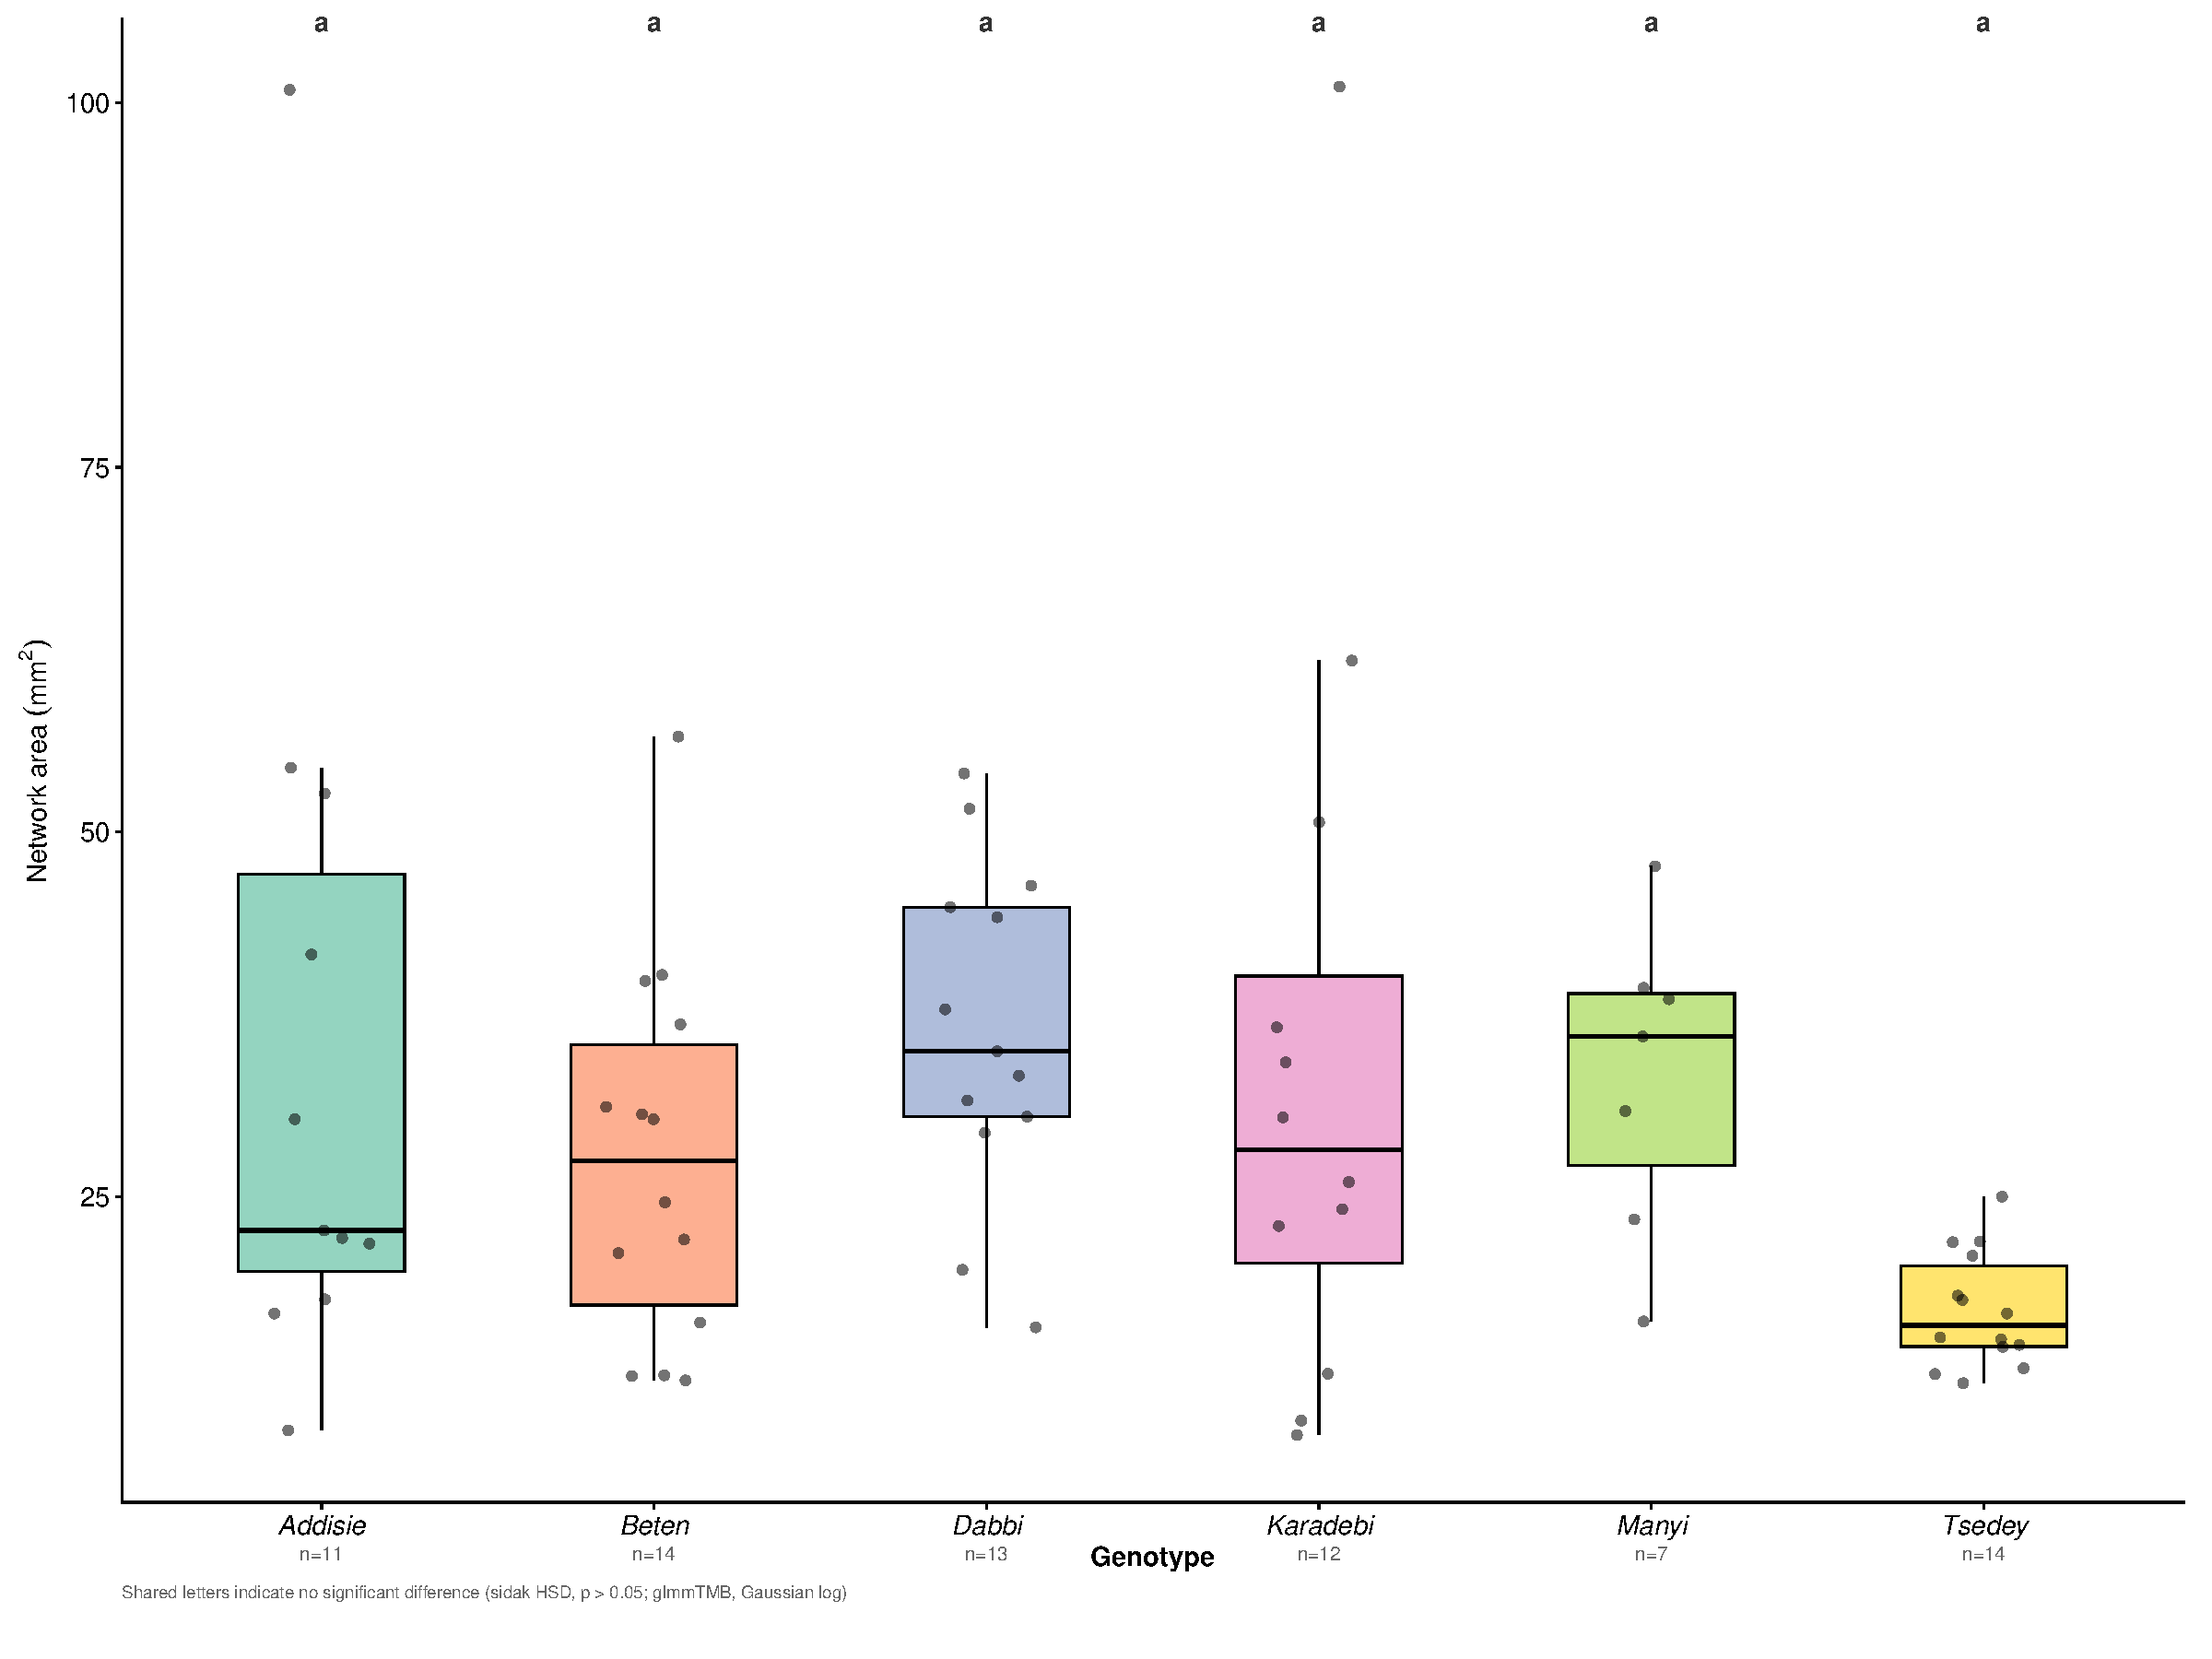
\includegraphics[keepaspectratio]{rsa_day1617_agar_files/figure-pdf/unnamed-chunk-6-10.pdf}}

\subsubsection{Solidity}\label{solidity}

\begin{Shaded}
\begin{Highlighting}[]
\CommentTok{\# ============================================================}
\CommentTok{\#  Solidity Analysis}
\CommentTok{\#  Solidity is a proportion (0–1) — Beta regression appropriate}
\CommentTok{\# ============================================================}

\CommentTok{\# ── 1. Inspect distribution ───────────────────────────────────}
\FunctionTok{summary}\NormalTok{(df}\SpecialCharTok{$}\NormalTok{Solidity)}
\end{Highlighting}
\end{Shaded}

\begin{verbatim}
   Min. 1st Qu.  Median    Mean 3rd Qu.    Max. 
0.02816 0.05195 0.07442 0.08242 0.10908 0.22140 
\end{verbatim}

\begin{Shaded}
\begin{Highlighting}[]
\FunctionTok{hist}\NormalTok{(df}\SpecialCharTok{$}\NormalTok{Solidity, }\AttributeTok{breaks =} \DecValTok{15}\NormalTok{, }\AttributeTok{main =} \StringTok{"Solidity distribution"}\NormalTok{)}
\end{Highlighting}
\end{Shaded}

\pandocbounded{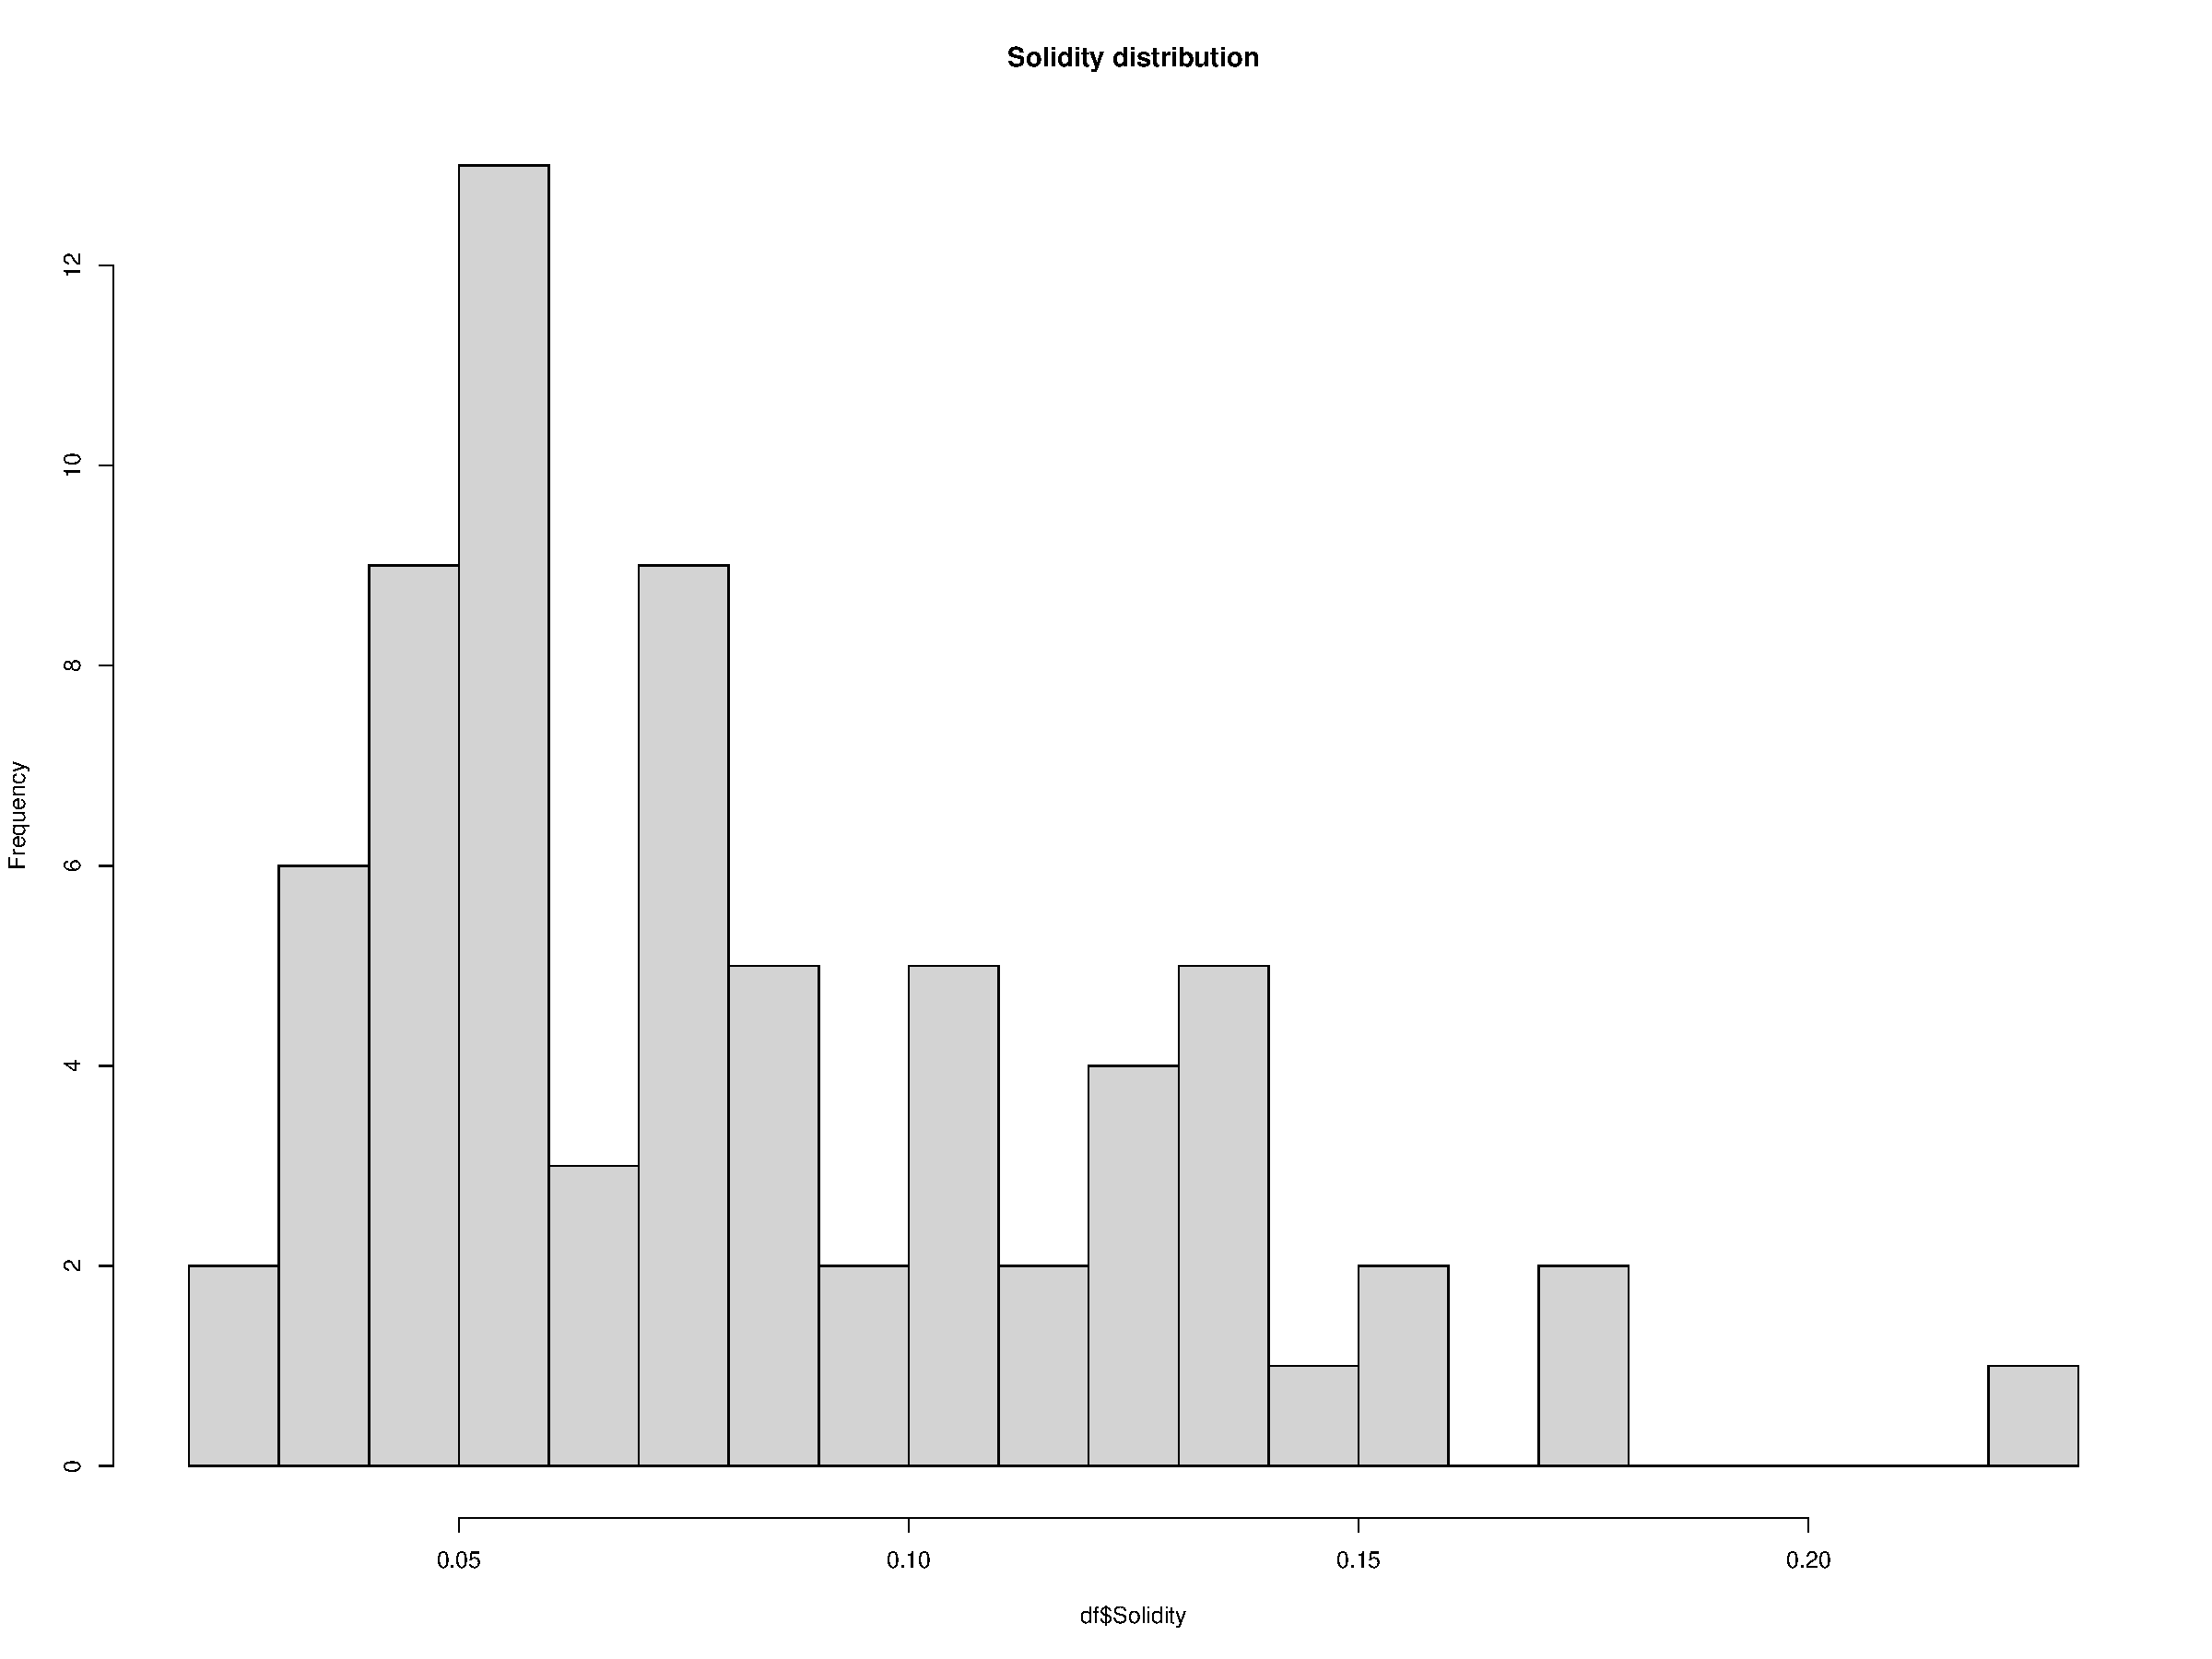
\includegraphics[keepaspectratio]{rsa_day1617_agar_files/figure-pdf/unnamed-chunk-7-1.pdf}}

\begin{Shaded}
\begin{Highlighting}[]
\CommentTok{\# Solidity is bounded 0–1 so Gaussian is inappropriate by definition}
\CommentTok{\# Beta family is the correct choice for proportions}


\CommentTok{\# ── 2. Check for exact 0s or 1s (Beta cannot handle these) ───}
\FunctionTok{sum}\NormalTok{(df}\SpecialCharTok{$}\NormalTok{Solidity }\SpecialCharTok{==} \DecValTok{0}\NormalTok{)}
\end{Highlighting}
\end{Shaded}

\begin{verbatim}
[1] 0
\end{verbatim}

\begin{Shaded}
\begin{Highlighting}[]
\FunctionTok{sum}\NormalTok{(df}\SpecialCharTok{$}\NormalTok{Solidity }\SpecialCharTok{==} \DecValTok{1}\NormalTok{)}
\end{Highlighting}
\end{Shaded}

\begin{verbatim}
[1] 0
\end{verbatim}

\begin{Shaded}
\begin{Highlighting}[]
\CommentTok{\# If any exist, apply small correction:}
\CommentTok{\# df$Solidity \textless{}{-} (df$Solidity * (nrow(df) {-} 1) + 0.5) / nrow(df)}


\CommentTok{\# ── 3. Fit full nested model ──────────────────────────────────}
\NormalTok{solidity\_tmb }\OtherTok{\textless{}{-}} \FunctionTok{glmmTMB}\NormalTok{(}
\NormalTok{  Solidity }\SpecialCharTok{\textasciitilde{}}\NormalTok{ Genotype }\SpecialCharTok{+}\NormalTok{ (}\DecValTok{1} \SpecialCharTok{|}\NormalTok{ Batch}\SpecialCharTok{/}\NormalTok{Plate}\SpecialCharTok{/}\NormalTok{Seed),}
  \AttributeTok{data =}\NormalTok{ df, }\AttributeTok{family =} \FunctionTok{beta\_family}\NormalTok{()}
\NormalTok{)}

\FunctionTok{VarCorr}\NormalTok{(solidity\_tmb)}
\end{Highlighting}
\end{Shaded}

\begin{verbatim}

Conditional model:
 Groups           Name        Std.Dev.  
 Seed:Plate:Batch (Intercept) 4.2056e-05
 Plate:Batch      (Intercept) 1.3756e-01
 Batch            (Intercept) 2.2459e-01
\end{verbatim}

\begin{Shaded}
\begin{Highlighting}[]
\FunctionTok{check\_singularity}\NormalTok{(solidity\_tmb)}
\end{Highlighting}
\end{Shaded}

\begin{verbatim}
[1] TRUE
\end{verbatim}

\begin{Shaded}
\begin{Highlighting}[]
\FunctionTok{summary}\NormalTok{(solidity\_tmb)}
\end{Highlighting}
\end{Shaded}

\begin{verbatim}
 Family: beta  ( logit )
Formula:          Solidity ~ Genotype + (1 | Batch/Plate/Seed)
Data: df

      AIC       BIC    logLik -2*log(L)  df.resid 
   -269.1    -246.5     144.5    -289.1        61 

Random effects:

Conditional model:
 Groups           Name        Variance  Std.Dev. 
 Seed:Plate:Batch (Intercept) 1.769e-09 4.206e-05
 Plate:Batch      (Intercept) 1.892e-02 1.376e-01
 Batch            (Intercept) 5.044e-02 2.246e-01
Number of obs: 71, groups:  Seed:Plate:Batch, 38; Plate:Batch, 18; Batch, 4

Dispersion parameter for beta family (): 78.3 

Conditional model:
                  Estimate Std. Error z value Pr(>|z|)    
(Intercept)      -2.573561   0.183294 -14.041   <2e-16 ***
GenotypeBeten     0.001284   0.179004   0.007    0.994    
GenotypeDabbi     0.098204   0.209838   0.468    0.640    
GenotypeKaradebi  0.141875   0.194452   0.730    0.466    
GenotypeManyi     0.330912   0.219803   1.505    0.132    
GenotypeTsedey    0.150883   0.187002   0.807    0.420    
---
Signif. codes:  0 '***' 0.001 '**' 0.01 '*' 0.05 '.' 0.1 ' ' 1
\end{verbatim}

\begin{Shaded}
\begin{Highlighting}[]
\CommentTok{\# singularity is true so will reduce the model }

\CommentTok{\# ── 3. Fit reduced model ──────────────────────────────────}
\NormalTok{solidity\_tmb }\OtherTok{\textless{}{-}} \FunctionTok{glmmTMB}\NormalTok{(}
\NormalTok{  Solidity }\SpecialCharTok{\textasciitilde{}}\NormalTok{ Genotype }\SpecialCharTok{+}\NormalTok{ (}\DecValTok{1} \SpecialCharTok{|}\NormalTok{ Batch}\SpecialCharTok{/}\NormalTok{Plate),}
  \AttributeTok{data =}\NormalTok{ df, }\AttributeTok{family =} \FunctionTok{beta\_family}\NormalTok{()}
\NormalTok{)}

\FunctionTok{VarCorr}\NormalTok{(solidity\_tmb)}
\end{Highlighting}
\end{Shaded}

\begin{verbatim}

Conditional model:
 Groups      Name        Std.Dev.
 Plate:Batch (Intercept) 0.13756 
 Batch       (Intercept) 0.22459 
\end{verbatim}

\begin{Shaded}
\begin{Highlighting}[]
\FunctionTok{check\_singularity}\NormalTok{(solidity\_tmb)}
\end{Highlighting}
\end{Shaded}

\begin{verbatim}
[1] FALSE
\end{verbatim}

\begin{Shaded}
\begin{Highlighting}[]
\FunctionTok{summary}\NormalTok{(solidity\_tmb)}
\end{Highlighting}
\end{Shaded}

\begin{verbatim}
 Family: beta  ( logit )
Formula:          Solidity ~ Genotype + (1 | Batch/Plate)
Data: df

      AIC       BIC    logLik -2*log(L)  df.resid 
   -271.1    -250.7     144.5    -289.1        62 

Random effects:

Conditional model:
 Groups      Name        Variance Std.Dev.
 Plate:Batch (Intercept) 0.01892  0.1376  
 Batch       (Intercept) 0.05044  0.2246  
Number of obs: 71, groups:  Plate:Batch, 18; Batch, 4

Dispersion parameter for beta family (): 78.3 

Conditional model:
                  Estimate Std. Error z value Pr(>|z|)    
(Intercept)      -2.573563   0.183294 -14.041   <2e-16 ***
GenotypeBeten     0.001286   0.179005   0.007    0.994    
GenotypeDabbi     0.098203   0.209838   0.468    0.640    
GenotypeKaradebi  0.141877   0.194452   0.730    0.466    
GenotypeManyi     0.330913   0.219803   1.505    0.132    
GenotypeTsedey    0.150885   0.187002   0.807    0.420    
---
Signif. codes:  0 '***' 0.001 '**' 0.01 '*' 0.05 '.' 0.1 ' ' 1
\end{verbatim}

\begin{Shaded}
\begin{Highlighting}[]
\CommentTok{\# singularity is false so happy to continue on to assumption checks}

\CommentTok{\# ── 5. Assumption checks ──────────────────────────────────────}
\NormalTok{sim\_res }\OtherTok{\textless{}{-}} \FunctionTok{simulateResiduals}\NormalTok{(solidity\_tmb, }\AttributeTok{n =} \DecValTok{1000}\NormalTok{)}
\FunctionTok{plot}\NormalTok{(sim\_res)                               }\CommentTok{\# QQ + residuals vs fitted}
\end{Highlighting}
\end{Shaded}

\pandocbounded{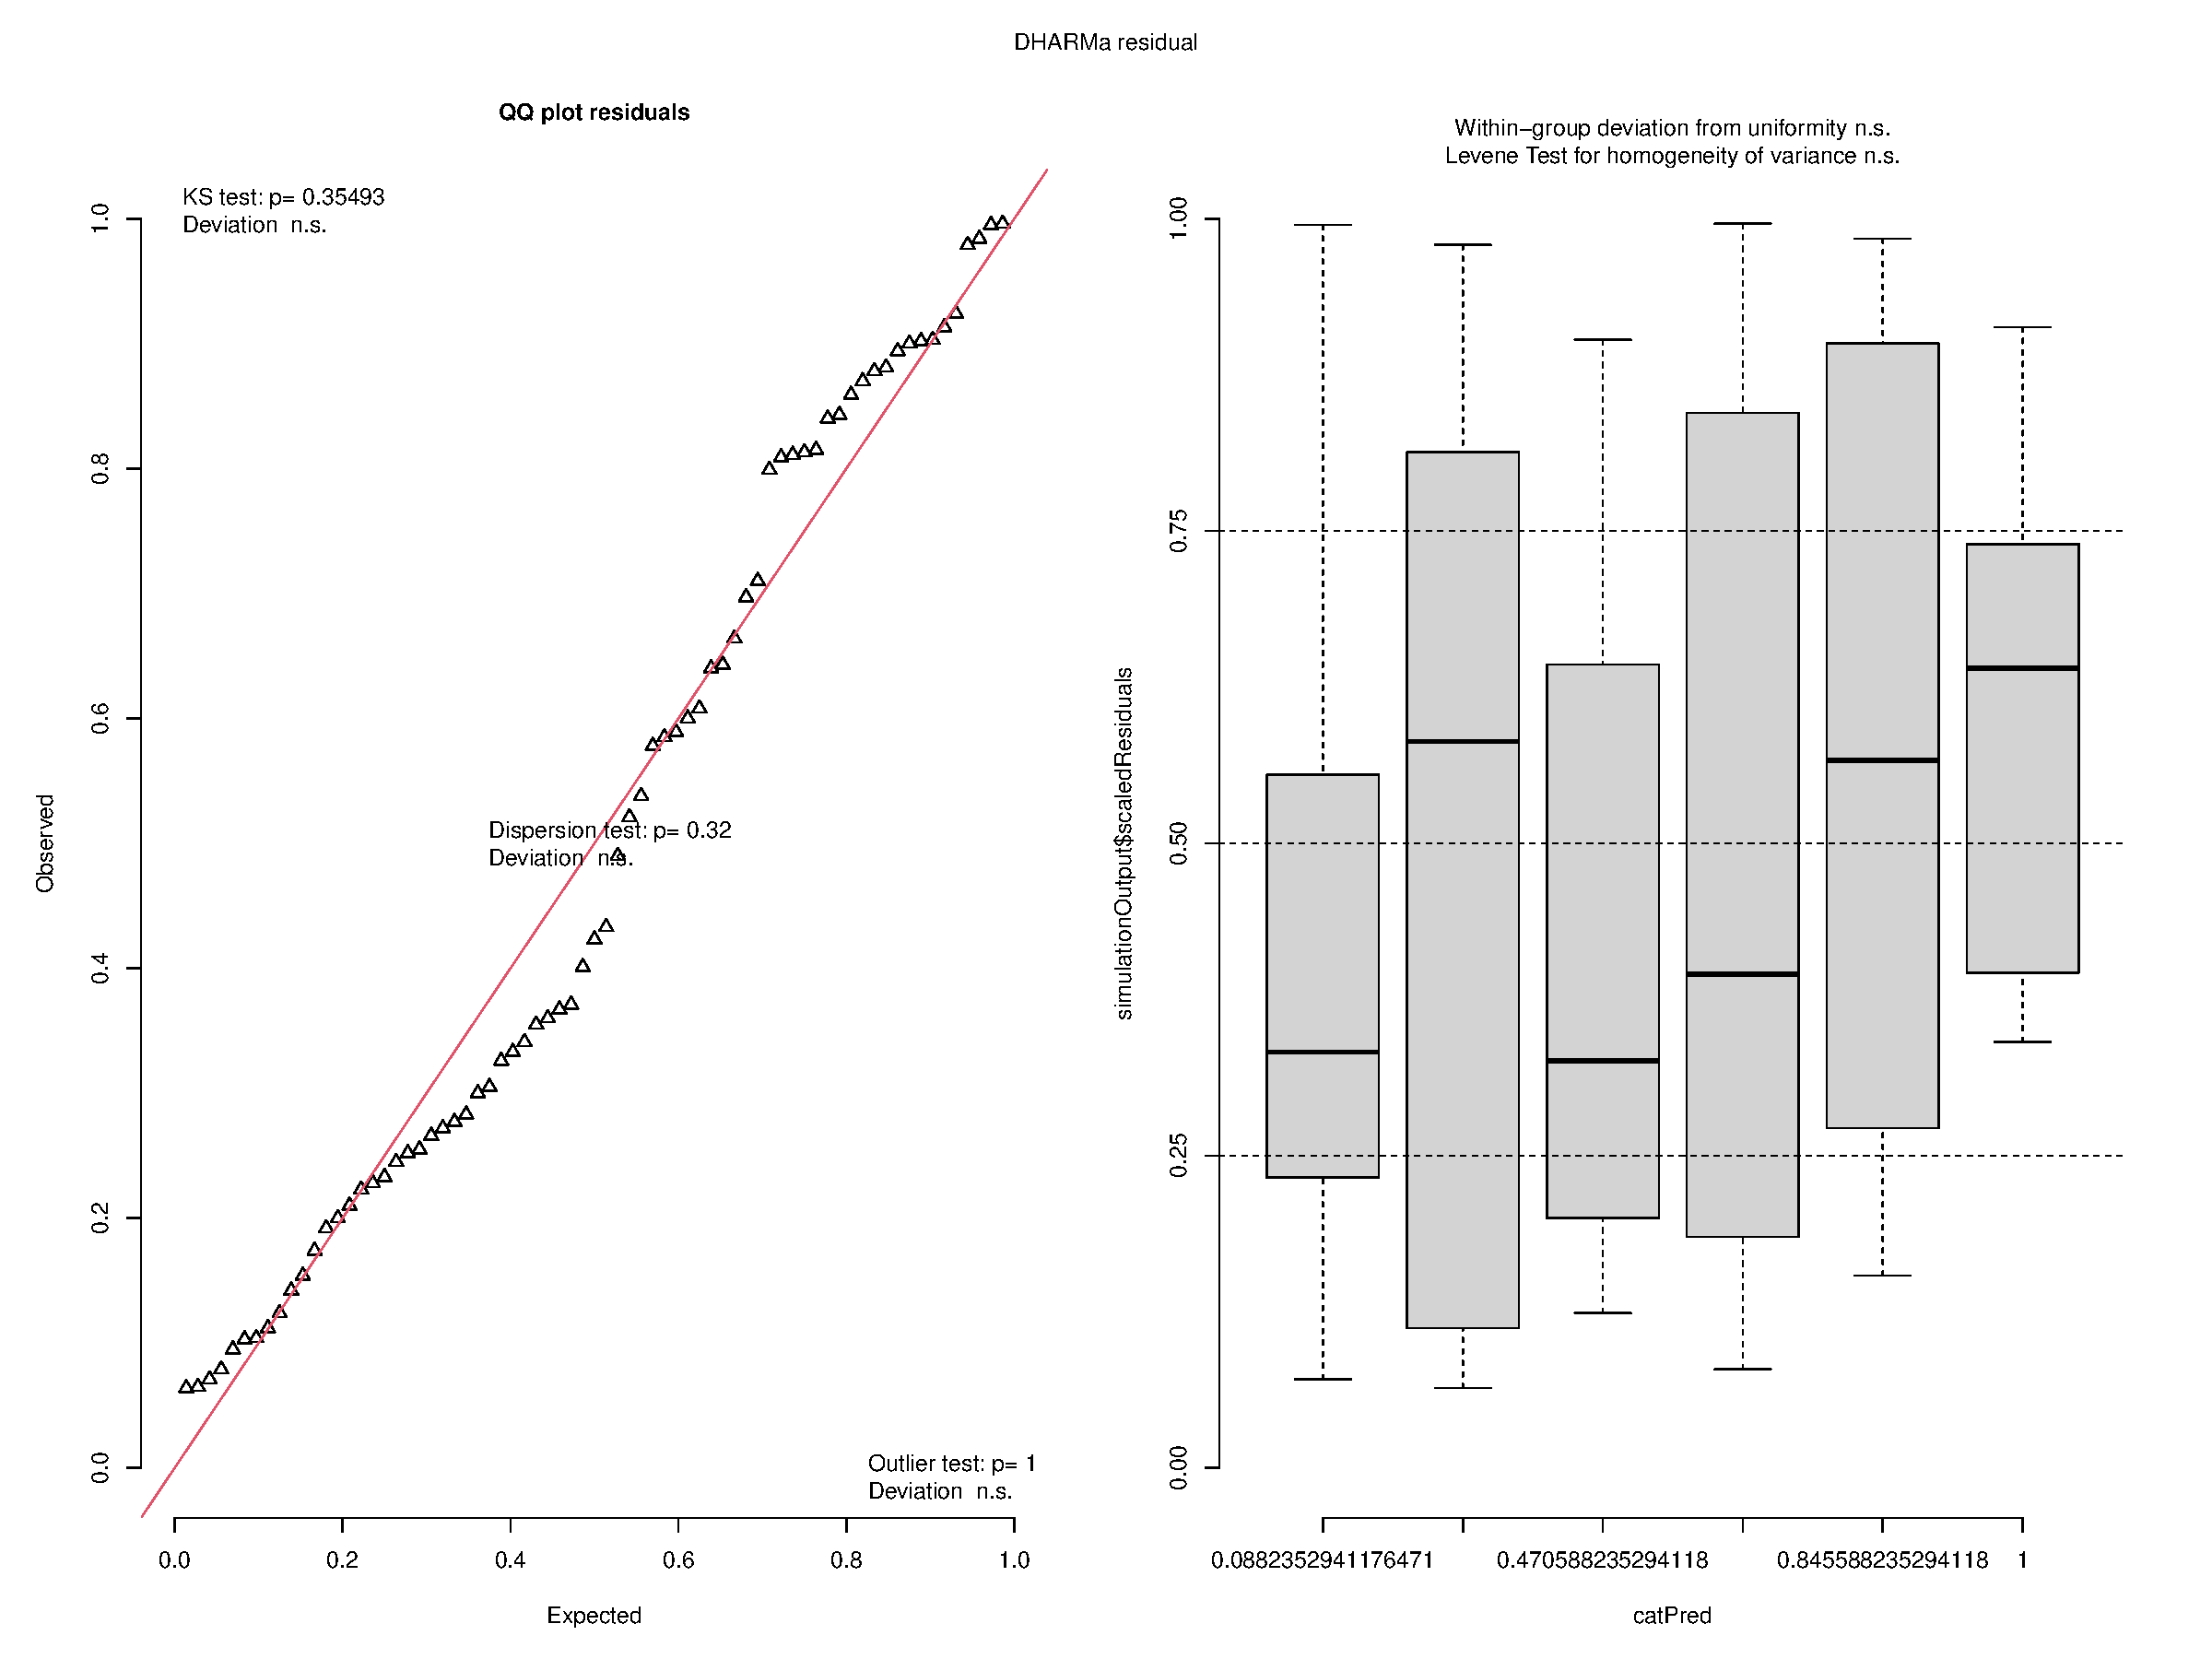
\includegraphics[keepaspectratio]{rsa_day1617_agar_files/figure-pdf/unnamed-chunk-7-2.pdf}}

\begin{Shaded}
\begin{Highlighting}[]
\FunctionTok{testUniformity}\NormalTok{(sim\_res)                     }\CommentTok{\# p \textgreater{} 0.05 = Beta appropriate}
\end{Highlighting}
\end{Shaded}

\pandocbounded{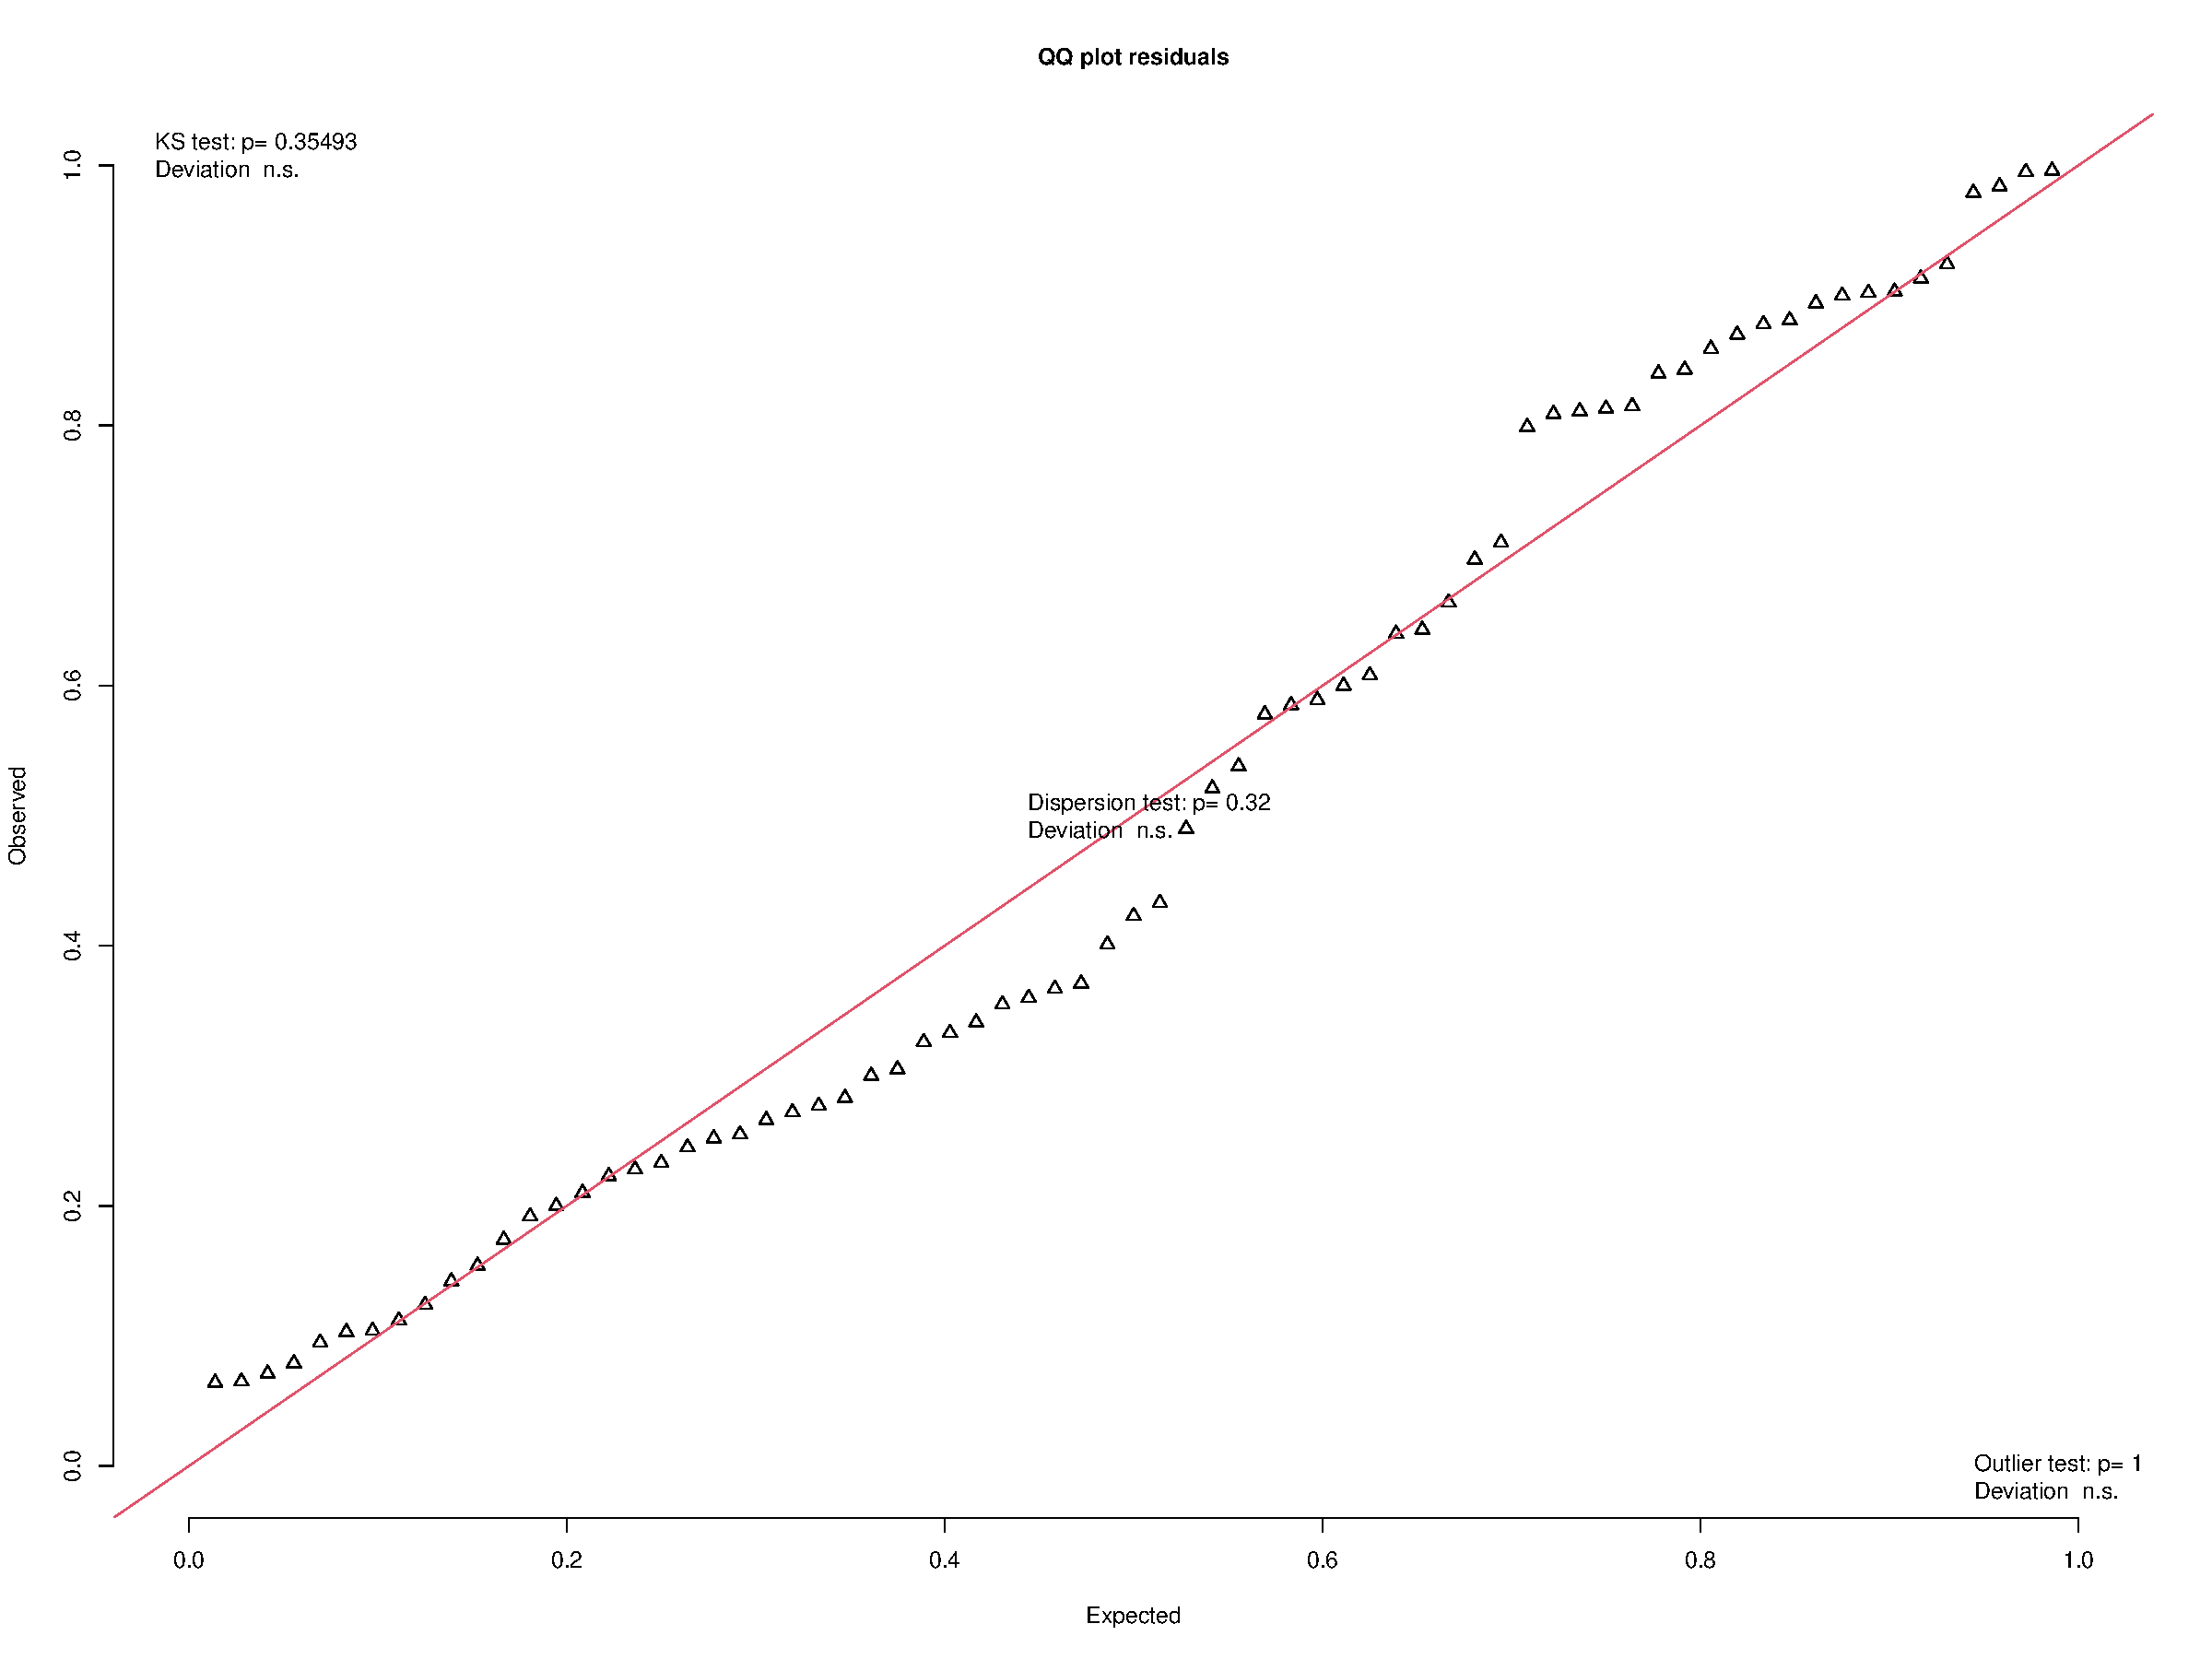
\includegraphics[keepaspectratio]{rsa_day1617_agar_files/figure-pdf/unnamed-chunk-7-3.pdf}}

\begin{verbatim}

    Exact one-sample Kolmogorov-Smirnov test

data:  simulationOutput$scaledResiduals
D = 0.10787, p-value = 0.3549
alternative hypothesis: two-sided
\end{verbatim}

\begin{Shaded}
\begin{Highlighting}[]
\FunctionTok{testDispersion}\NormalTok{(sim\_res)                     }\CommentTok{\# ratio ≈ 1.0}
\end{Highlighting}
\end{Shaded}

\pandocbounded{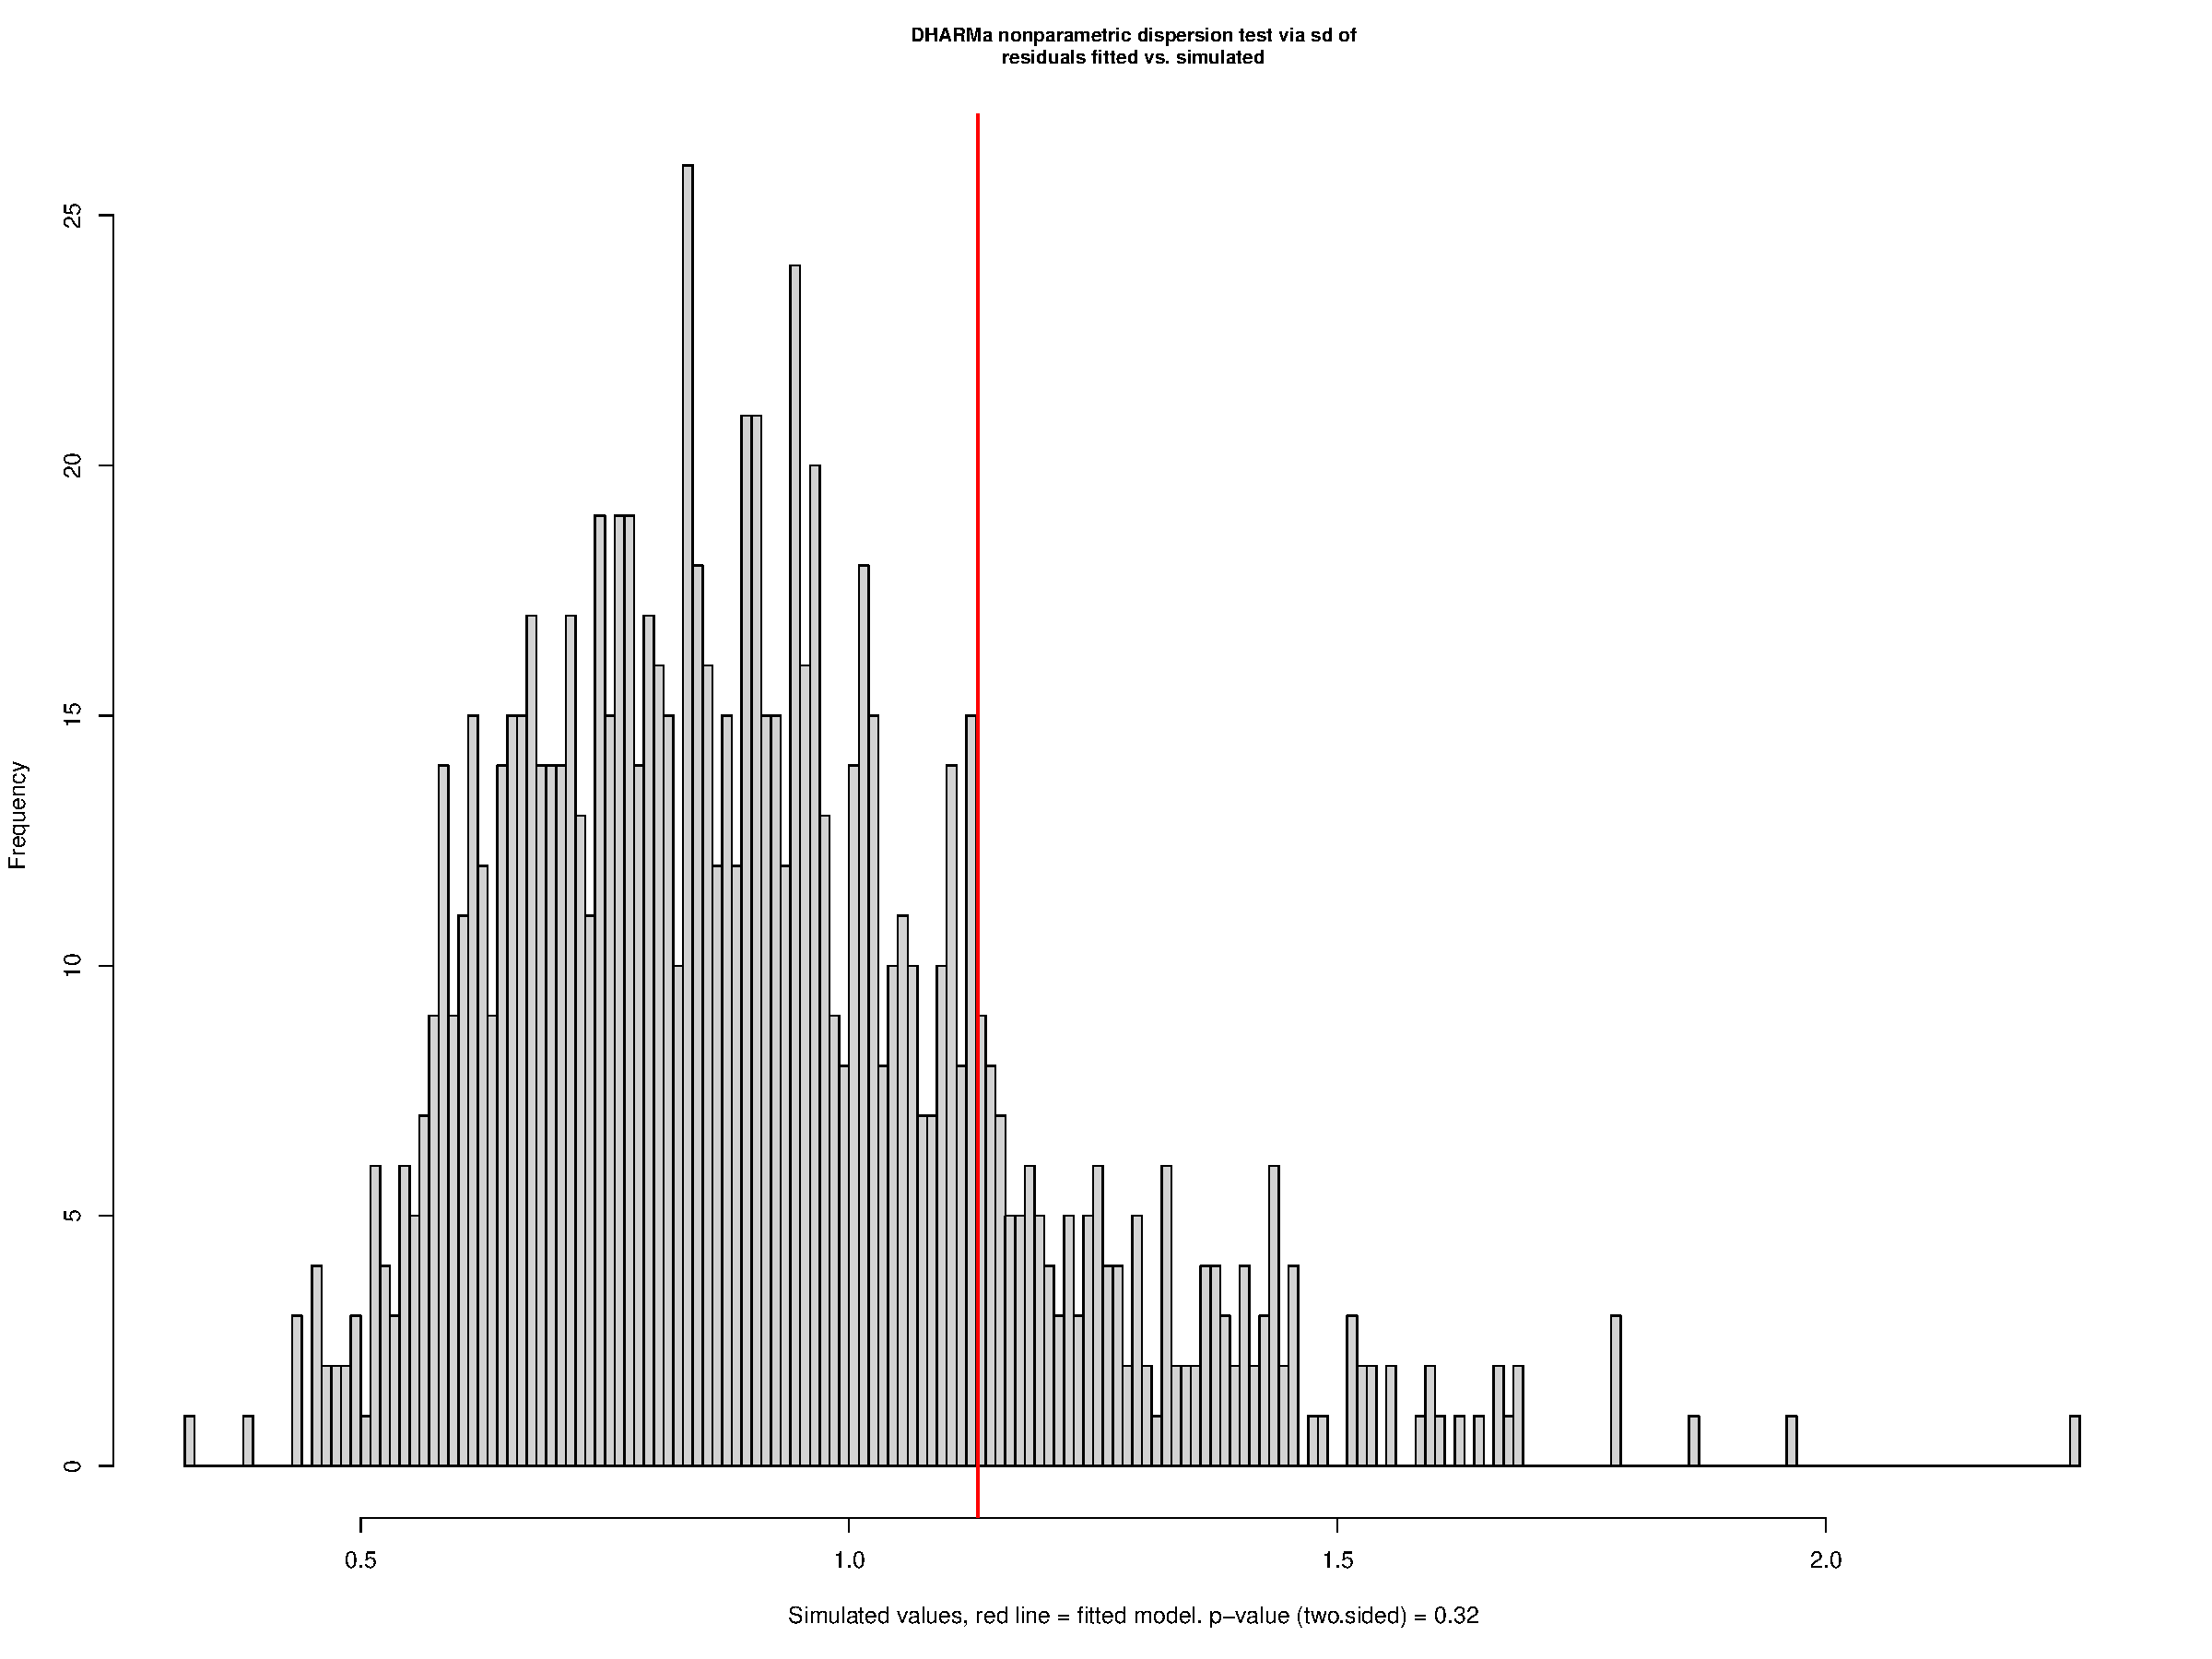
\includegraphics[keepaspectratio]{rsa_day1617_agar_files/figure-pdf/unnamed-chunk-7-4.pdf}}

\begin{verbatim}

    DHARMa nonparametric dispersion test via sd of residuals fitted vs.
    simulated

data:  simulationOutput
dispersion = 1.2486, p-value = 0.32
alternative hypothesis: two.sided
\end{verbatim}

\begin{Shaded}
\begin{Highlighting}[]
\FunctionTok{plotResiduals}\NormalTok{(sim\_res, }\AttributeTok{form =}\NormalTok{ df}\SpecialCharTok{$}\NormalTok{Genotype)  }\CommentTok{\# no patterns per genotype}
\end{Highlighting}
\end{Shaded}

\pandocbounded{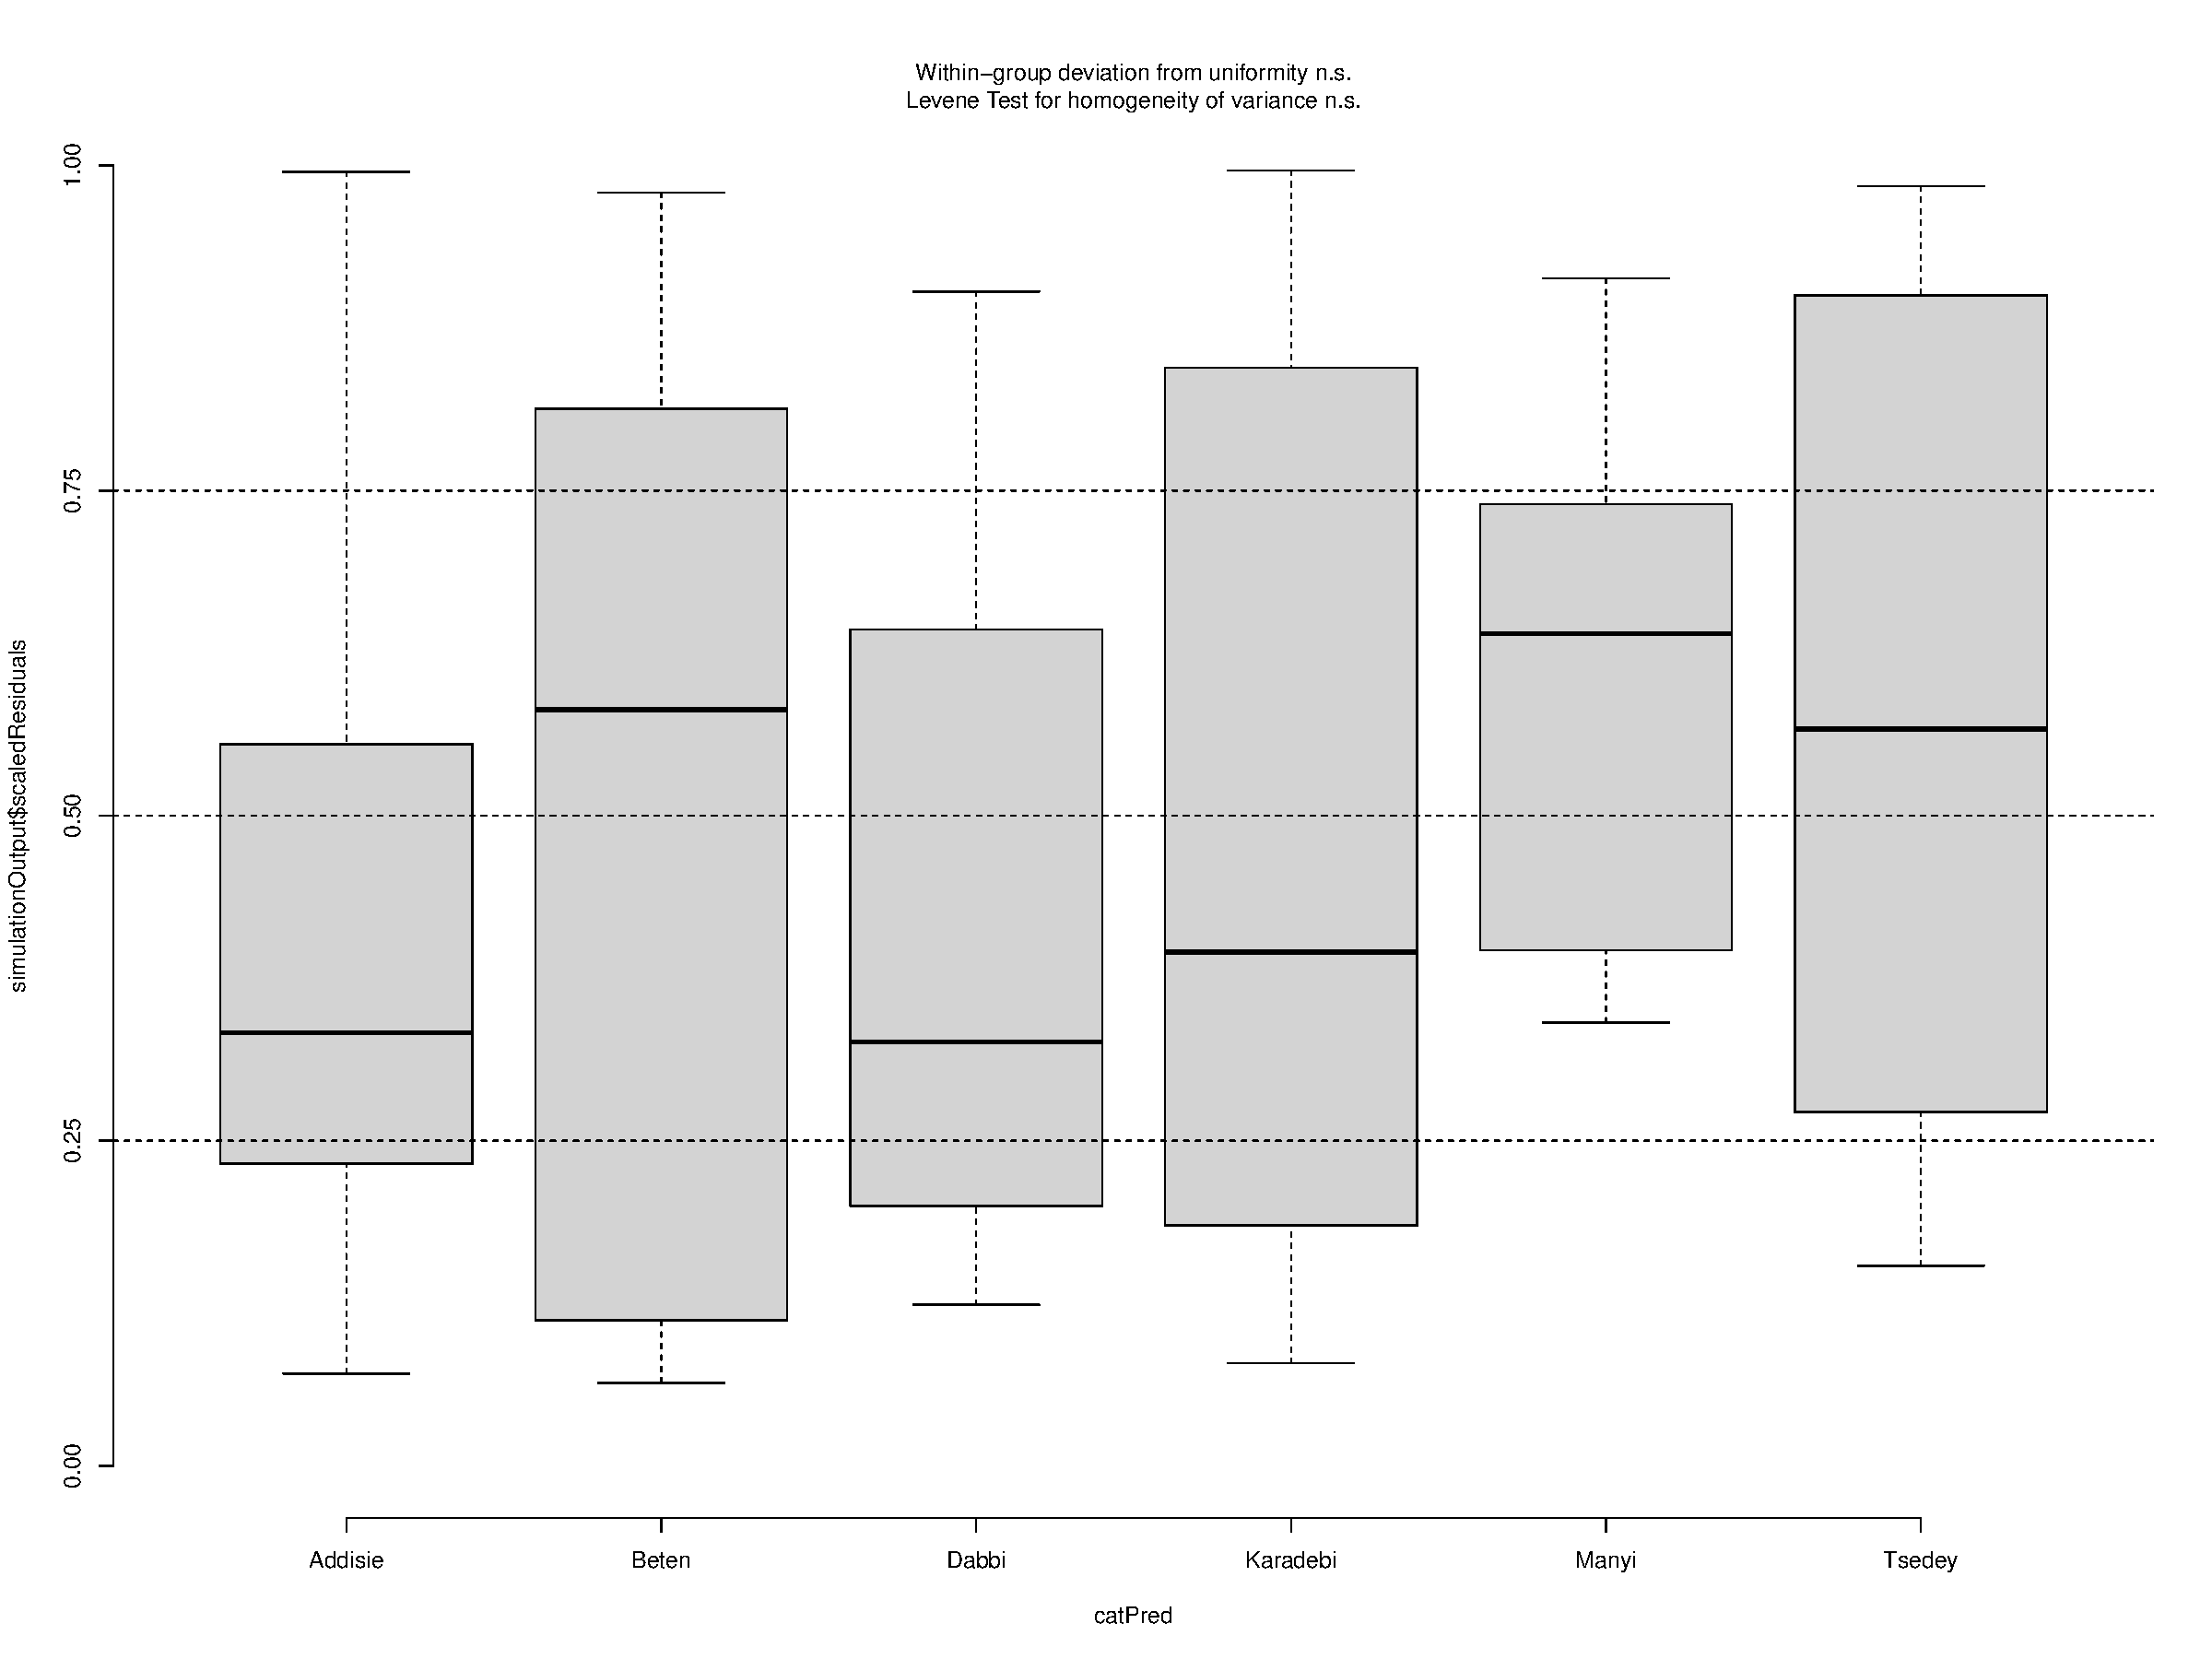
\includegraphics[keepaspectratio]{rsa_day1617_agar_files/figure-pdf/unnamed-chunk-7-5.pdf}}

\begin{Shaded}
\begin{Highlighting}[]
\CommentTok{\# assumptions all look good so happy to continue }

\CommentTok{\# ── 6. Test overall Genotype effect ──────────────────────────}
\NormalTok{car}\SpecialCharTok{::}\FunctionTok{Anova}\NormalTok{(solidity\_tmb, }\AttributeTok{type =} \StringTok{"III"}\NormalTok{)}
\end{Highlighting}
\end{Shaded}

\begin{verbatim}
Analysis of Deviance Table (Type III Wald chisquare tests)

Response: Solidity
               Chisq Df Pr(>Chisq)    
(Intercept) 197.1388  1     <2e-16 ***
Genotype      3.3194  5     0.6509    
---
Signif. codes:  0 '***' 0.001 '**' 0.01 '*' 0.05 '.' 0.1 ' ' 1
\end{verbatim}

\begin{Shaded}
\begin{Highlighting}[]
\CommentTok{\# ── 7. Pairwise comparisons + CLD ────────────────────────────}
\CommentTok{\# type = "response" back{-}transforms from logit link to 0{-}1 scale}
\NormalTok{emm }\OtherTok{\textless{}{-}} \FunctionTok{emmeans}\NormalTok{(solidity\_tmb, }\SpecialCharTok{\textasciitilde{}}\NormalTok{ Genotype, }\AttributeTok{type =} \StringTok{"response"}\NormalTok{)}
\FunctionTok{pairs}\NormalTok{(emm, }\AttributeTok{adjust =} \StringTok{"sidak"}\NormalTok{)}
\end{Highlighting}
\end{Shaded}

\begin{verbatim}
 contrast           odds.ratio    SE  df null z.ratio p.value
 Addisie / Beten         0.999 0.179 Inf    1  -0.007  1.0000
 Addisie / Dabbi         0.906 0.190 Inf    1  -0.468  1.0000
 Addisie / Karadebi      0.868 0.169 Inf    1  -0.730  0.9999
 Addisie / Manyi         0.718 0.158 Inf    1  -1.505  0.8808
 Addisie / Tsedey        0.860 0.161 Inf    1  -0.807  0.9997
 Beten / Dabbi           0.908 0.172 Inf    1  -0.510  1.0000
 Beten / Karadebi        0.869 0.152 Inf    1  -0.803  0.9997
 Beten / Manyi           0.719 0.141 Inf    1  -1.681  0.7681
 Beten / Tsedey          0.861 0.144 Inf    1  -0.893  0.9991
 Dabbi / Karadebi        0.957 0.168 Inf    1  -0.248  1.0000
 Dabbi / Manyi           0.792 0.154 Inf    1  -1.199  0.9803
 Dabbi / Tsedey          0.949 0.184 Inf    1  -0.271  1.0000
 Karadebi / Manyi        0.828 0.155 Inf    1  -1.011  0.9963
 Karadebi / Tsedey       0.991 0.173 Inf    1  -0.051  1.0000
 Manyi / Tsedey          1.197 0.219 Inf    1   0.985  0.9972

P value adjustment: sidak method for 15 tests 
Tests are performed on the log odds ratio scale 
\end{verbatim}

\begin{Shaded}
\begin{Highlighting}[]
\NormalTok{cld\_df }\OtherTok{\textless{}{-}} \FunctionTok{as.data.frame}\NormalTok{(}\FunctionTok{cld}\NormalTok{(emm, }\AttributeTok{adjust =} \StringTok{"sidak"}\NormalTok{,}
                             \AttributeTok{Letters =}\NormalTok{ letters, }\AttributeTok{alpha =} \FloatTok{0.05}\NormalTok{)) }\SpecialCharTok{\%\textgreater{}\%}
  \FunctionTok{mutate}\NormalTok{(}\AttributeTok{.group =} \FunctionTok{trimws}\NormalTok{(.group))}

\NormalTok{n\_df }\OtherTok{\textless{}{-}}\NormalTok{ df }\SpecialCharTok{\%\textgreater{}\%}
  \FunctionTok{count}\NormalTok{(Genotype) }\SpecialCharTok{\%\textgreater{}\%}
  \FunctionTok{mutate}\NormalTok{(}\AttributeTok{label =} \FunctionTok{paste0}\NormalTok{(}\StringTok{"n="}\NormalTok{, n))}


\CommentTok{\# ── 8. Plot 1 — Boxplot ───────────────────────────────────────}

\CommentTok{\# ── Solidity plot — y{-}axis zoomed to data range ───────────────}

\NormalTok{y\_ceil }\OtherTok{\textless{}{-}} \FunctionTok{max}\NormalTok{(df}\SpecialCharTok{$}\NormalTok{Solidity) }\SpecialCharTok{*} \FloatTok{1.22}
\NormalTok{y\_label }\OtherTok{\textless{}{-}}\NormalTok{ y\_ceil }\SpecialCharTok{*} \FloatTok{0.95}

\NormalTok{p1 }\OtherTok{\textless{}{-}} \FunctionTok{ggplot}\NormalTok{(df, }\FunctionTok{aes}\NormalTok{(}\AttributeTok{x =}\NormalTok{ Genotype, }\AttributeTok{y =}\NormalTok{ Solidity, }\AttributeTok{fill =}\NormalTok{ Genotype)) }\SpecialCharTok{+}

  \FunctionTok{geom\_boxplot}\NormalTok{(}
    \AttributeTok{alpha         =} \FloatTok{0.7}\NormalTok{,}
    \AttributeTok{outlier.shape =} \ConstantTok{NA}\NormalTok{,}
    \AttributeTok{width         =} \FloatTok{0.5}\NormalTok{,}
    \AttributeTok{colour        =} \StringTok{"black"}\NormalTok{,}
    \AttributeTok{linewidth     =} \FloatTok{0.5}
\NormalTok{  ) }\SpecialCharTok{+}

  \FunctionTok{geom\_jitter}\NormalTok{(}
    \AttributeTok{width  =} \FloatTok{0.15}\NormalTok{,}
    \AttributeTok{size   =} \FloatTok{1.8}\NormalTok{,}
    \AttributeTok{alpha  =} \FloatTok{0.55}\NormalTok{,}
    \AttributeTok{colour =} \StringTok{"black"}
\NormalTok{  ) }\SpecialCharTok{+}

  \FunctionTok{geom\_text}\NormalTok{(}
    \AttributeTok{data        =}\NormalTok{ cld\_df,}
    \FunctionTok{aes}\NormalTok{(}\AttributeTok{x =}\NormalTok{ Genotype, }\AttributeTok{label =}\NormalTok{ .group),}
    \AttributeTok{y           =}\NormalTok{ y\_label,}
    \AttributeTok{inherit.aes =} \ConstantTok{FALSE}\NormalTok{,}
    \AttributeTok{size        =} \DecValTok{5}\NormalTok{,}
    \AttributeTok{fontface    =} \StringTok{"bold"}\NormalTok{,}
    \AttributeTok{colour      =} \StringTok{"grey20"}
\NormalTok{  ) }\SpecialCharTok{+}

  \FunctionTok{geom\_text}\NormalTok{(}
    \AttributeTok{data        =}\NormalTok{ n\_df,}
    \FunctionTok{aes}\NormalTok{(}\AttributeTok{x =}\NormalTok{ Genotype, }\AttributeTok{label =}\NormalTok{ label),}
    \AttributeTok{y           =} \SpecialCharTok{{-}}\ConstantTok{Inf}\NormalTok{,}
    \AttributeTok{vjust       =} \FloatTok{4.2}\NormalTok{,}
    \AttributeTok{inherit.aes =} \ConstantTok{FALSE}\NormalTok{,}
    \AttributeTok{size        =} \FloatTok{3.5}\NormalTok{,}
    \AttributeTok{colour      =} \StringTok{"grey40"}
\NormalTok{  ) }\SpecialCharTok{+}

  \FunctionTok{scale\_fill\_brewer}\NormalTok{(}\AttributeTok{palette =} \StringTok{"Set2"}\NormalTok{) }\SpecialCharTok{+}

  \FunctionTok{labs}\NormalTok{(}
    \AttributeTok{x       =} \StringTok{"Genotype"}\NormalTok{,}
    \AttributeTok{y       =} \StringTok{"Solidity (proportion)"}\NormalTok{,}
    \AttributeTok{caption =} \StringTok{"Shared letters indicate no significant difference (sidak HSD, p \textgreater{} 0.05; glmmTMB, Beta)"}
\NormalTok{  ) }\SpecialCharTok{+}

  \FunctionTok{theme\_classic}\NormalTok{(}\AttributeTok{base\_size =} \DecValTok{14}\NormalTok{) }\SpecialCharTok{+}
  \FunctionTok{theme}\NormalTok{(}
    \AttributeTok{legend.position =} \StringTok{"none"}\NormalTok{,}
    \AttributeTok{axis.line       =} \FunctionTok{element\_line}\NormalTok{(}\AttributeTok{colour =} \StringTok{"black"}\NormalTok{, }\AttributeTok{linewidth =} \FloatTok{0.6}\NormalTok{),}
    \AttributeTok{axis.ticks      =} \FunctionTok{element\_line}\NormalTok{(}\AttributeTok{colour =} \StringTok{"black"}\NormalTok{, }\AttributeTok{linewidth =} \FloatTok{0.5}\NormalTok{),}
    \AttributeTok{axis.title      =} \FunctionTok{element\_text}\NormalTok{(}\AttributeTok{size =} \DecValTok{14}\NormalTok{, }\AttributeTok{face =} \StringTok{"bold"}\NormalTok{),}
    \AttributeTok{axis.text       =} \FunctionTok{element\_text}\NormalTok{(}\AttributeTok{size =} \DecValTok{14}\NormalTok{, }\AttributeTok{colour =} \StringTok{"black"}\NormalTok{),}
    \AttributeTok{axis.text.x     =} \FunctionTok{element\_text}\NormalTok{(}\AttributeTok{face =} \StringTok{"italic"}\NormalTok{, }\AttributeTok{margin =} \FunctionTok{margin}\NormalTok{(}\AttributeTok{t =} \DecValTok{3}\NormalTok{)),}
    \AttributeTok{plot.caption    =} \FunctionTok{element\_text}\NormalTok{(}\AttributeTok{size =} \DecValTok{9}\NormalTok{, }\AttributeTok{colour =} \StringTok{"grey40"}\NormalTok{, }\AttributeTok{hjust =} \DecValTok{0}\NormalTok{),}
    \AttributeTok{plot.margin     =} \FunctionTok{margin}\NormalTok{(}\AttributeTok{t =} \DecValTok{10}\NormalTok{, }\AttributeTok{r =} \DecValTok{15}\NormalTok{, }\AttributeTok{b =} \DecValTok{30}\NormalTok{, }\AttributeTok{l =} \DecValTok{10}\NormalTok{)}
\NormalTok{  )}

\NormalTok{p1 }\SpecialCharTok{+} \FunctionTok{coord\_cartesian}\NormalTok{(}
  \AttributeTok{ylim =} \FunctionTok{c}\NormalTok{(}\DecValTok{0}\NormalTok{, }\FunctionTok{max}\NormalTok{(df}\SpecialCharTok{$}\NormalTok{Solidity) }\SpecialCharTok{*} \FloatTok{1.22}\NormalTok{),}
  \AttributeTok{clip =} \StringTok{"off"}
\NormalTok{)}
\end{Highlighting}
\end{Shaded}

\pandocbounded{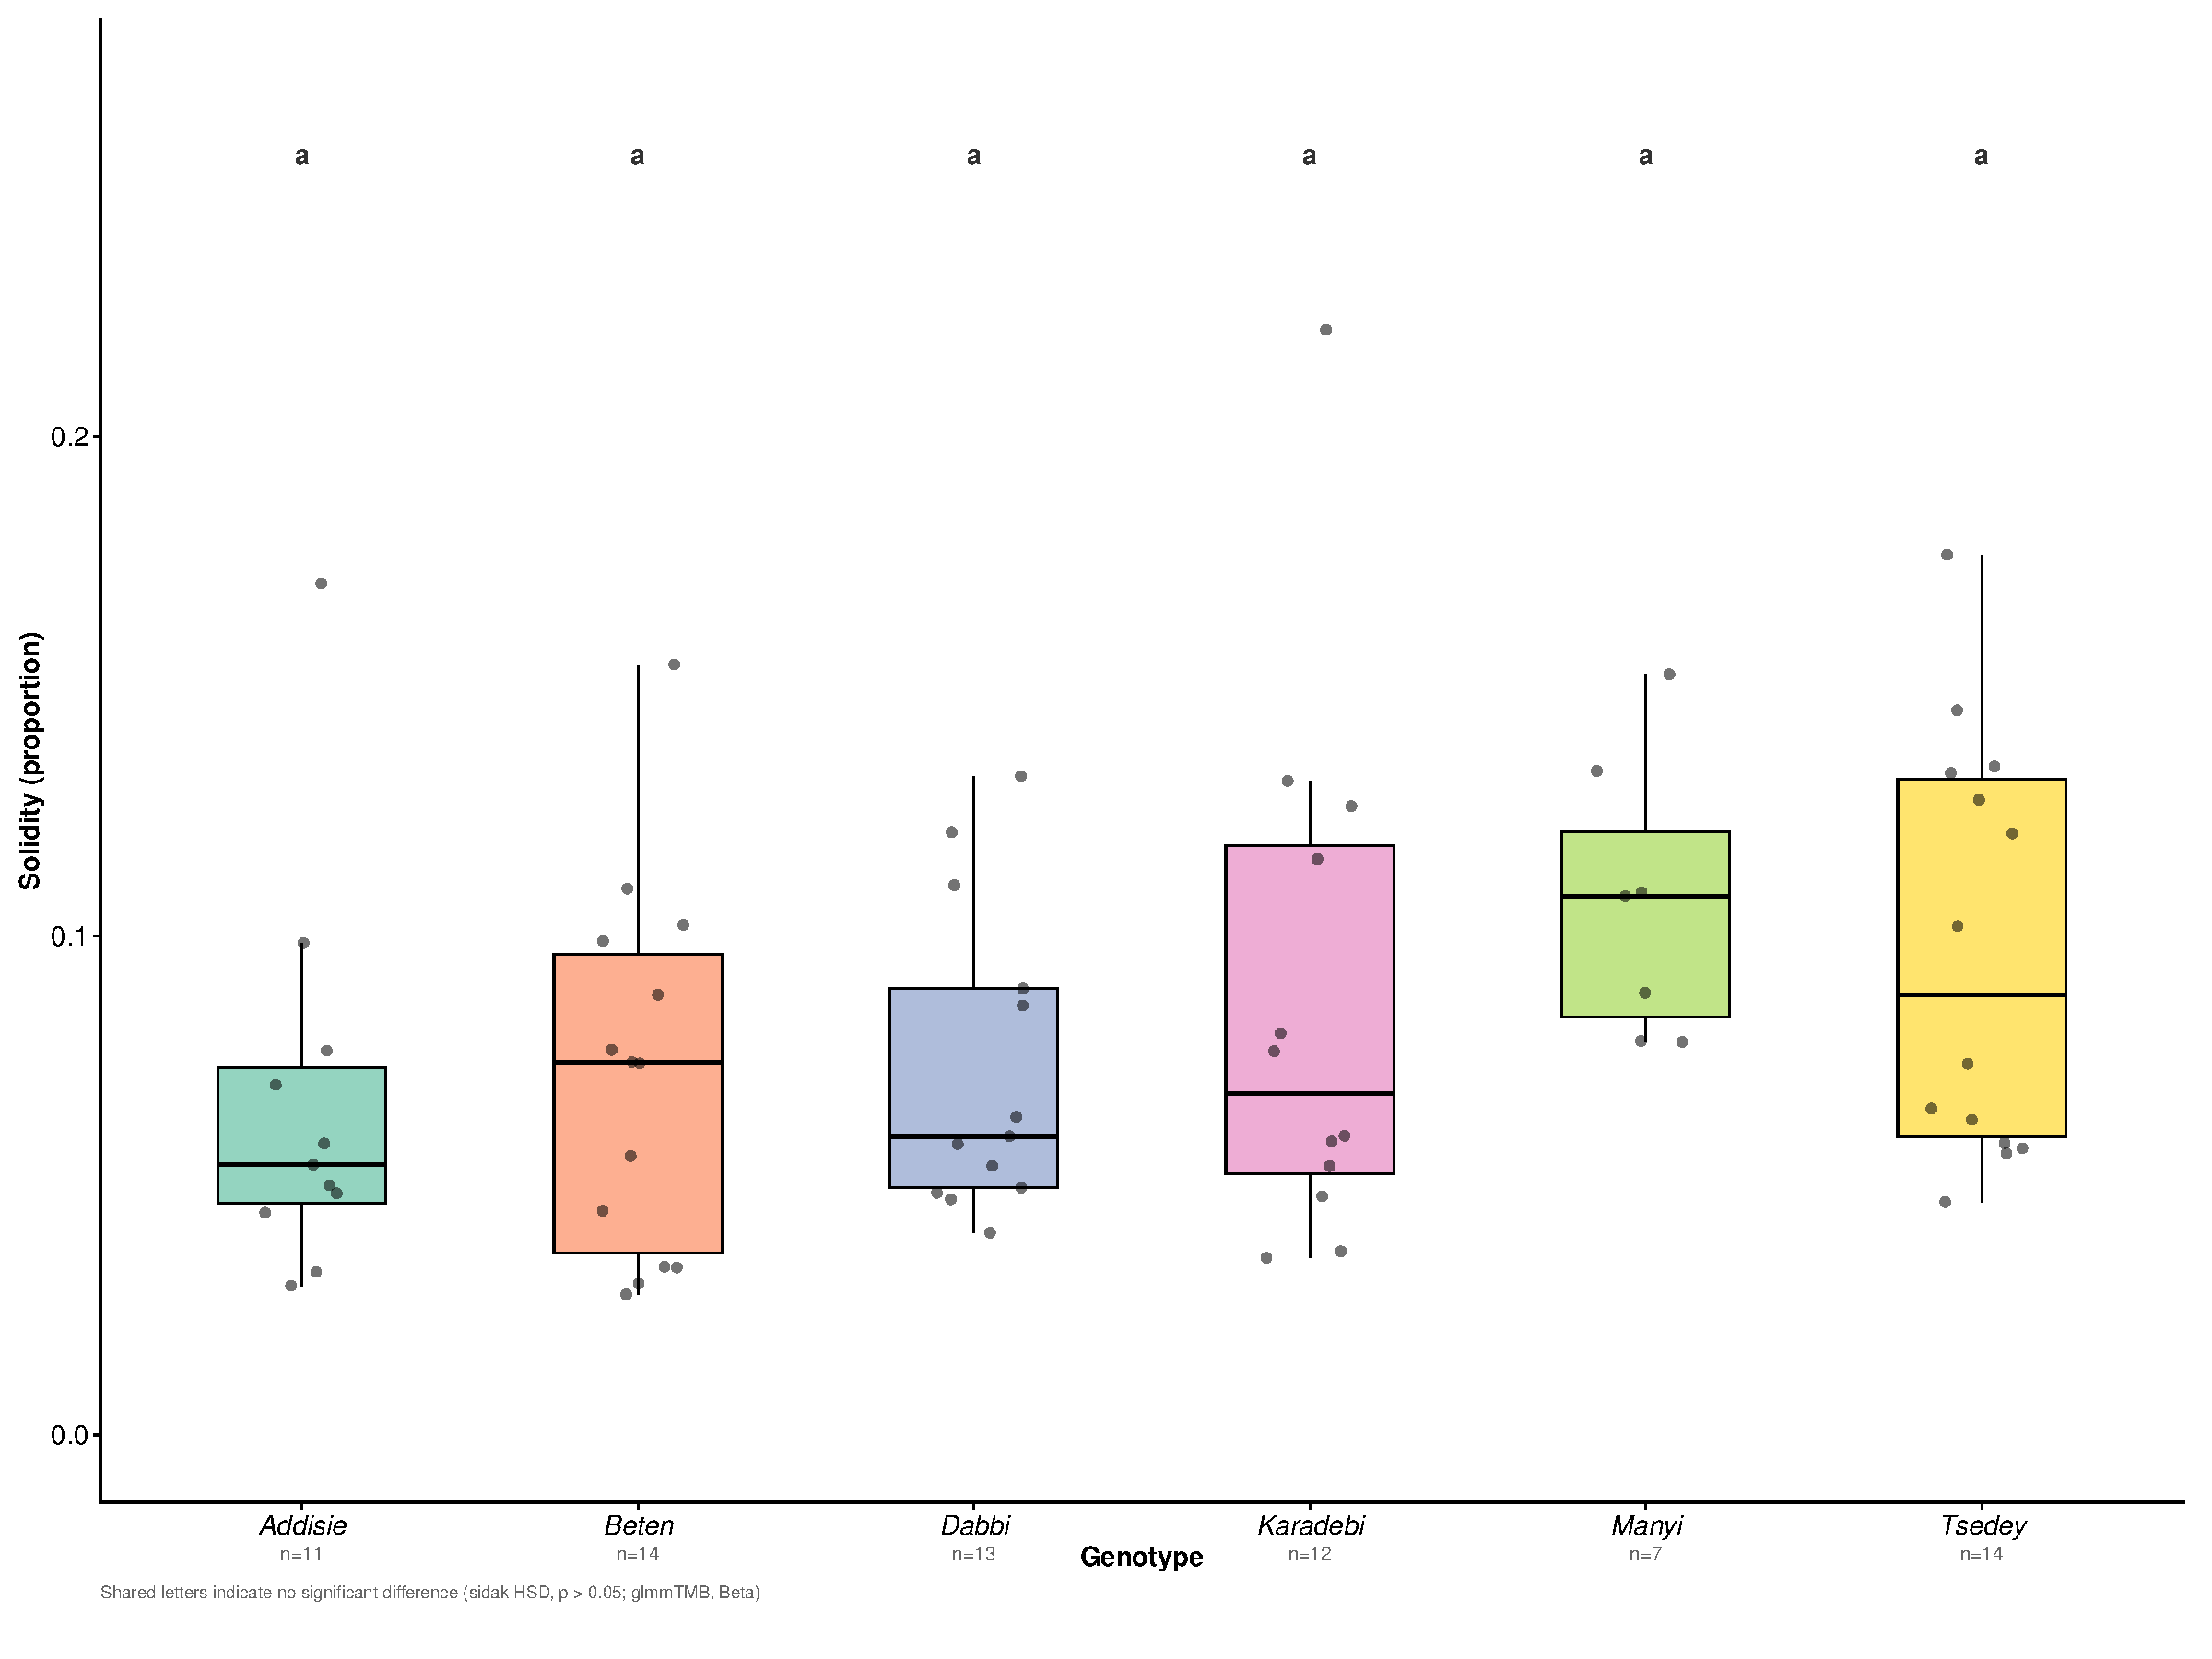
\includegraphics[keepaspectratio]{rsa_day1617_agar_files/figure-pdf/unnamed-chunk-7-6.pdf}}

\subsubsection{Width to Depth Ratio}\label{width-to-depth-ratio}

\begin{Shaded}
\begin{Highlighting}[]
\CommentTok{\# ============================================================}
\CommentTok{\#  Width{-}to{-}Depth Ratio Analysis}
\CommentTok{\#  Ratio data — positive continuous, likely right{-}skewed}
\CommentTok{\#  Start raw, log{-}transform only if DHARMa flags poor fit}
\CommentTok{\# ============================================================}

\CommentTok{\# ── 1. Inspect distribution ───────────────────────────────────}
\FunctionTok{summary}\NormalTok{(df}\SpecialCharTok{$}\StringTok{\textasciigrave{}}\AttributeTok{Width.to.Depth.Ratio}\StringTok{\textasciigrave{}}\NormalTok{)}
\end{Highlighting}
\end{Shaded}

\begin{verbatim}
   Min. 1st Qu.  Median    Mean 3rd Qu.    Max. 
0.08108 0.16650 0.23014 0.28198 0.34860 0.75703 
\end{verbatim}

\begin{Shaded}
\begin{Highlighting}[]
\FunctionTok{class}\NormalTok{(df}\SpecialCharTok{$}\StringTok{\textasciigrave{}}\AttributeTok{Width.to.Depth.Ratio}\StringTok{\textasciigrave{}}\NormalTok{)}
\end{Highlighting}
\end{Shaded}

\begin{verbatim}
[1] "numeric"
\end{verbatim}

\begin{Shaded}
\begin{Highlighting}[]
\FunctionTok{hist}\NormalTok{(df}\SpecialCharTok{$}\StringTok{\textasciigrave{}}\AttributeTok{Width.to.Depth.Ratio}\StringTok{\textasciigrave{}}\NormalTok{, }\AttributeTok{breaks =} \DecValTok{15}\NormalTok{, }\AttributeTok{main =} \StringTok{"Width{-}to{-}Depth Ratio distribution"}\NormalTok{)}
\end{Highlighting}
\end{Shaded}

\pandocbounded{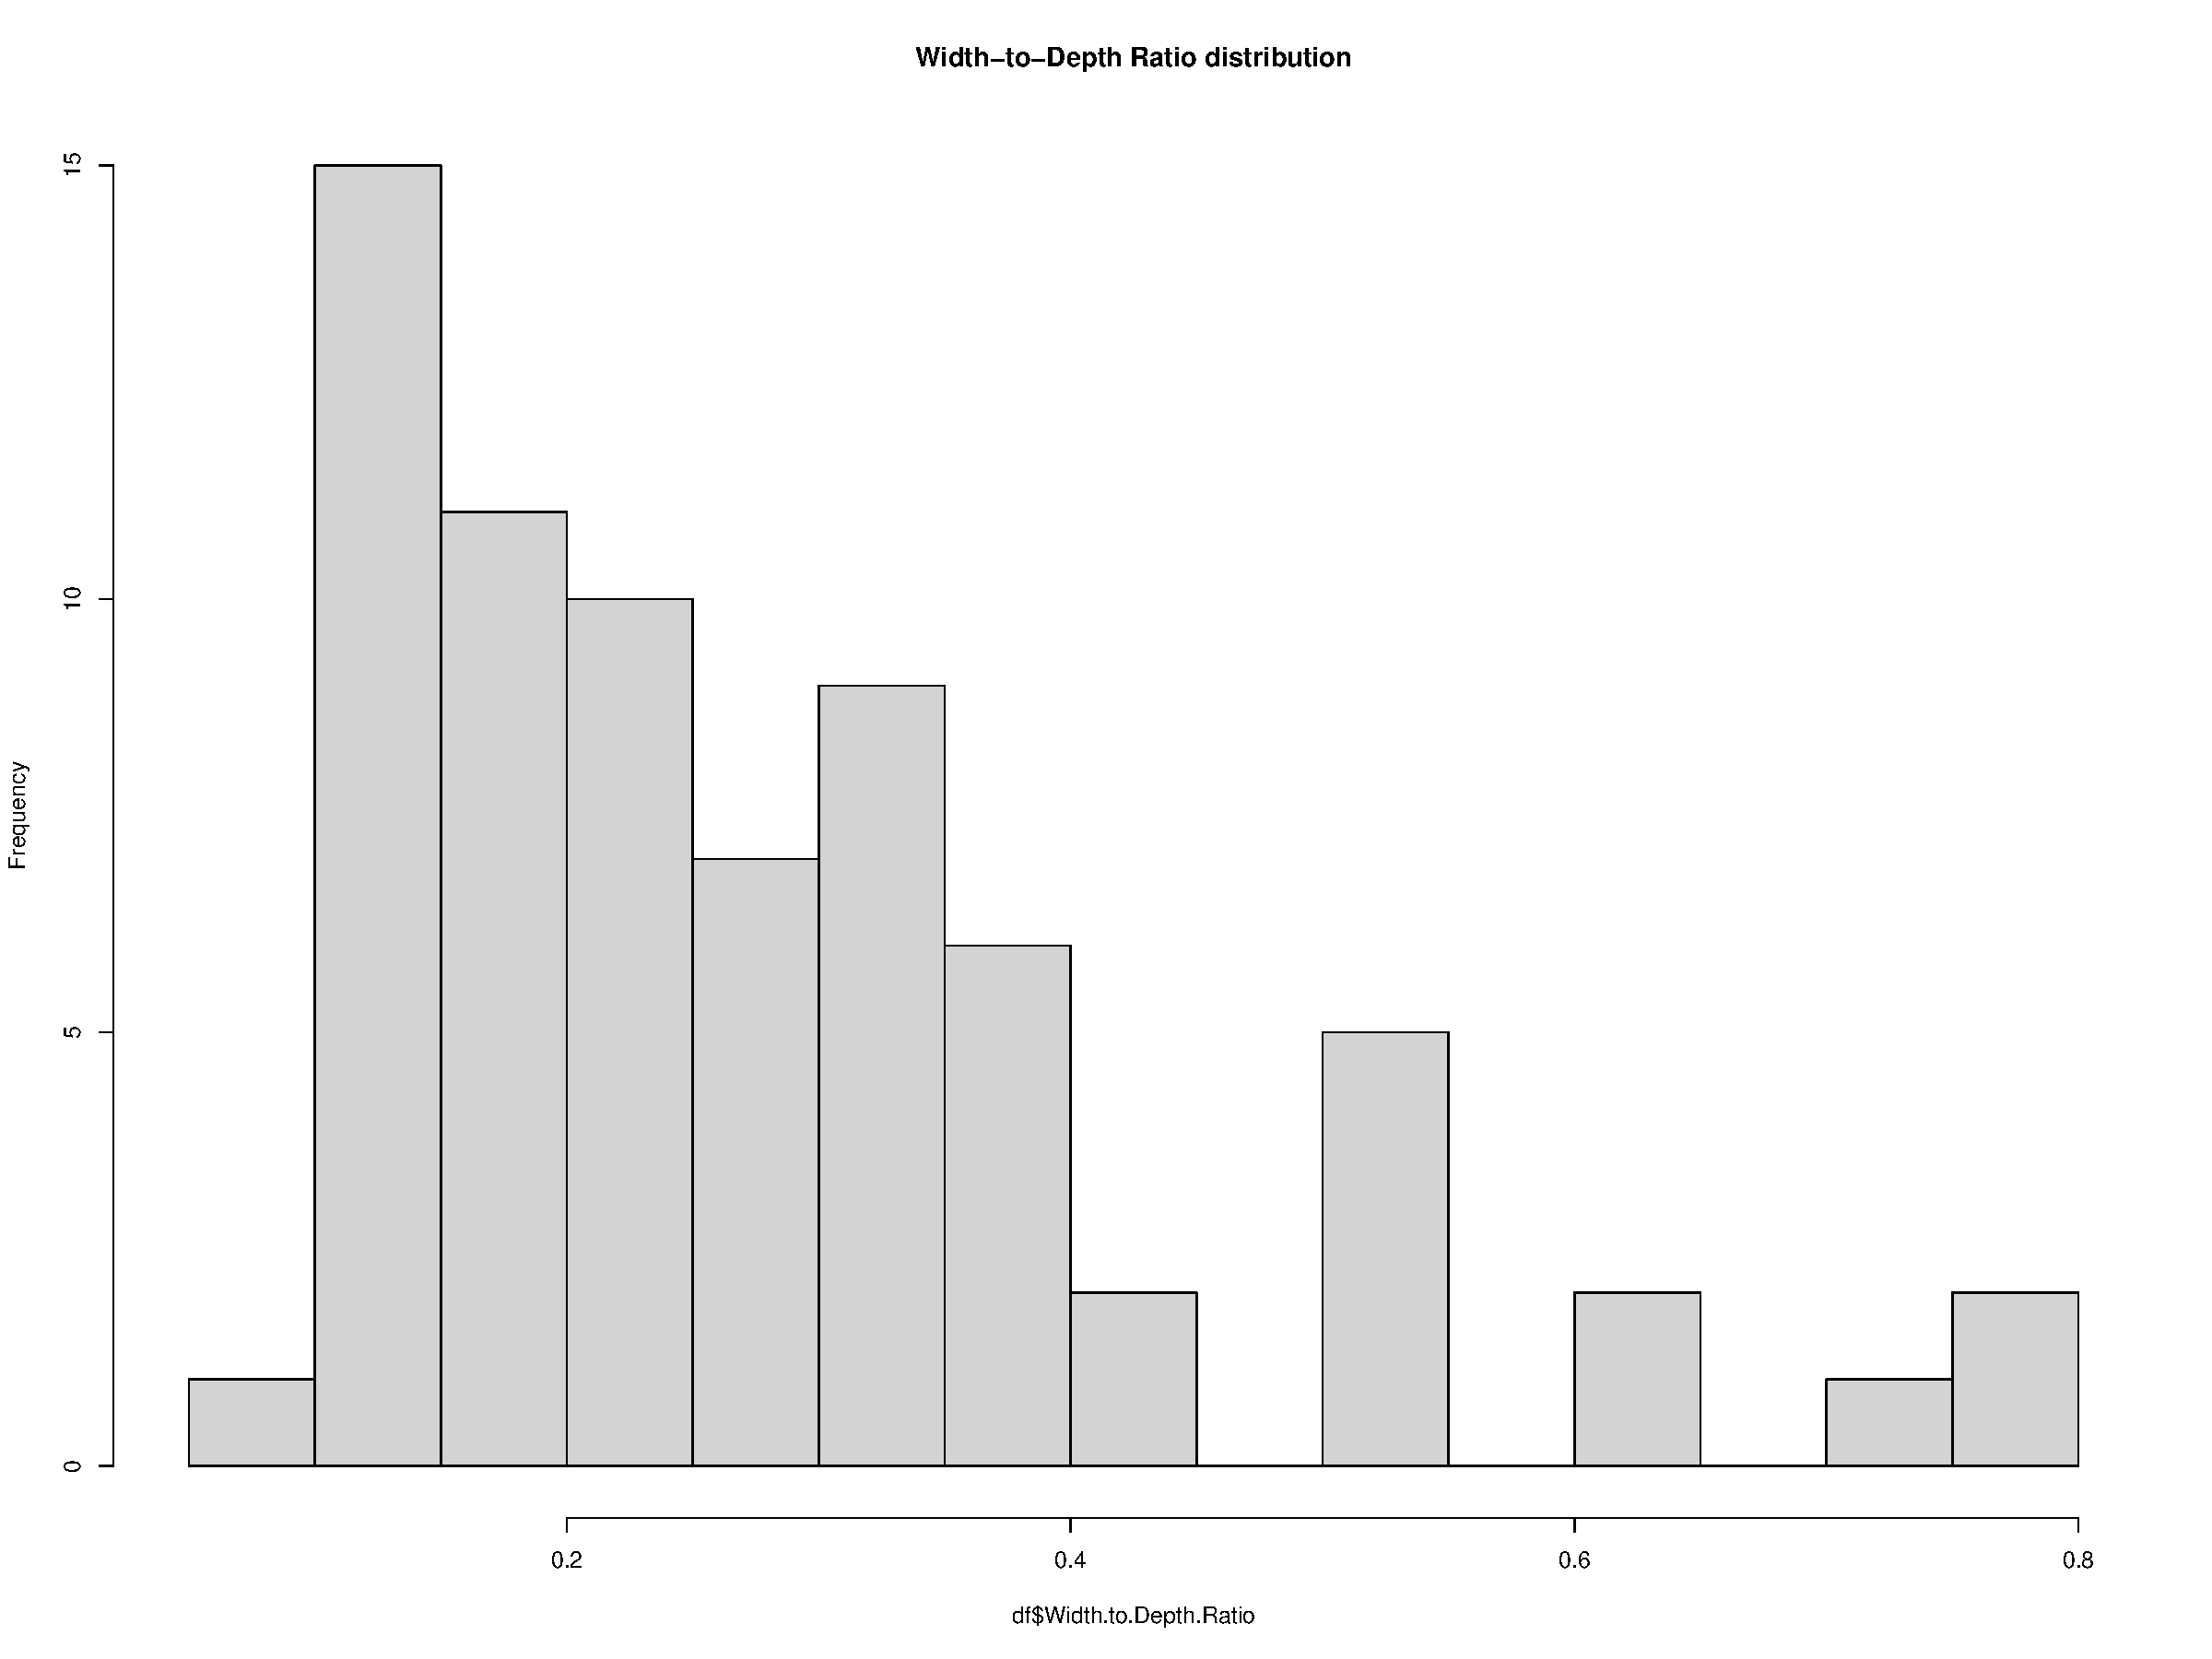
\includegraphics[keepaspectratio]{rsa_day1617_agar_files/figure-pdf/unnamed-chunk-8-1.pdf}}

\begin{Shaded}
\begin{Highlighting}[]
\CommentTok{\# ── 2. Fit full nested model on raw scale ────────────────────}
\NormalTok{wdr\_full }\OtherTok{\textless{}{-}} \FunctionTok{glmmTMB}\NormalTok{(}
  \StringTok{\textasciigrave{}}\AttributeTok{Width.to.Depth.Ratio}\StringTok{\textasciigrave{}} \SpecialCharTok{\textasciitilde{}}\NormalTok{ Genotype }\SpecialCharTok{+}\NormalTok{ (}\DecValTok{1} \SpecialCharTok{|}\NormalTok{ Batch}\SpecialCharTok{/}\NormalTok{Plate}\SpecialCharTok{/}\NormalTok{Seed),}
  \AttributeTok{data =}\NormalTok{ df, }\AttributeTok{family =} \FunctionTok{gaussian}\NormalTok{()}
\NormalTok{)}

\FunctionTok{VarCorr}\NormalTok{(wdr\_full)}
\end{Highlighting}
\end{Shaded}

\begin{verbatim}

Conditional model:
 Groups           Name        Std.Dev.  
 Seed:Plate:Batch (Intercept) 2.8226e-06
 Plate:Batch      (Intercept) 2.0563e-06
 Batch            (Intercept) 5.0767e-09
 Residual                     1.5393e-01
\end{verbatim}

\begin{Shaded}
\begin{Highlighting}[]
\FunctionTok{check\_singularity}\NormalTok{(wdr\_full)}
\end{Highlighting}
\end{Shaded}

\begin{verbatim}
[1] TRUE
\end{verbatim}

\begin{Shaded}
\begin{Highlighting}[]
\FunctionTok{summary}\NormalTok{(wdr\_full)}
\end{Highlighting}
\end{Shaded}

\begin{verbatim}
 Family: gaussian  ( identity )
Formula:          Width.to.Depth.Ratio ~ Genotype + (1 | Batch/Plate/Seed)
Data: df

      AIC       BIC    logLik -2*log(L)  df.resid 
    -44.2     -21.6      32.1     -64.2        61 

Random effects:

Conditional model:
 Groups           Name        Variance  Std.Dev. 
 Seed:Plate:Batch (Intercept) 7.967e-12 2.823e-06
 Plate:Batch      (Intercept) 4.228e-12 2.056e-06
 Batch            (Intercept) 2.577e-17 5.077e-09
 Residual                     2.369e-02 1.539e-01
Number of obs: 71, groups:  Seed:Plate:Batch, 38; Plate:Batch, 18; Batch, 4

Dispersion estimate for gaussian family (sigma^2): 0.0237 

Conditional model:
                 Estimate Std. Error z value Pr(>|z|)
(Intercept)       0.34641        NaN     NaN      NaN
GenotypeBeten    -0.04901        NaN     NaN      NaN
GenotypeDabbi    -0.08217        NaN     NaN      NaN
GenotypeKaradebi -0.02795        NaN     NaN      NaN
GenotypeManyi    -0.07353        NaN     NaN      NaN
GenotypeTsedey   -0.14072        NaN     NaN      NaN
\end{verbatim}

\begin{Shaded}
\begin{Highlighting}[]
\CommentTok{\# check assumptions }
\NormalTok{sim\_res }\OtherTok{\textless{}{-}} \FunctionTok{simulateResiduals}\NormalTok{(wdr\_full, }\AttributeTok{n =} \DecValTok{1000}\NormalTok{)}
\FunctionTok{plot}\NormalTok{(sim\_res)                               }\CommentTok{\# QQ + residuals vs fitted}
\end{Highlighting}
\end{Shaded}

\pandocbounded{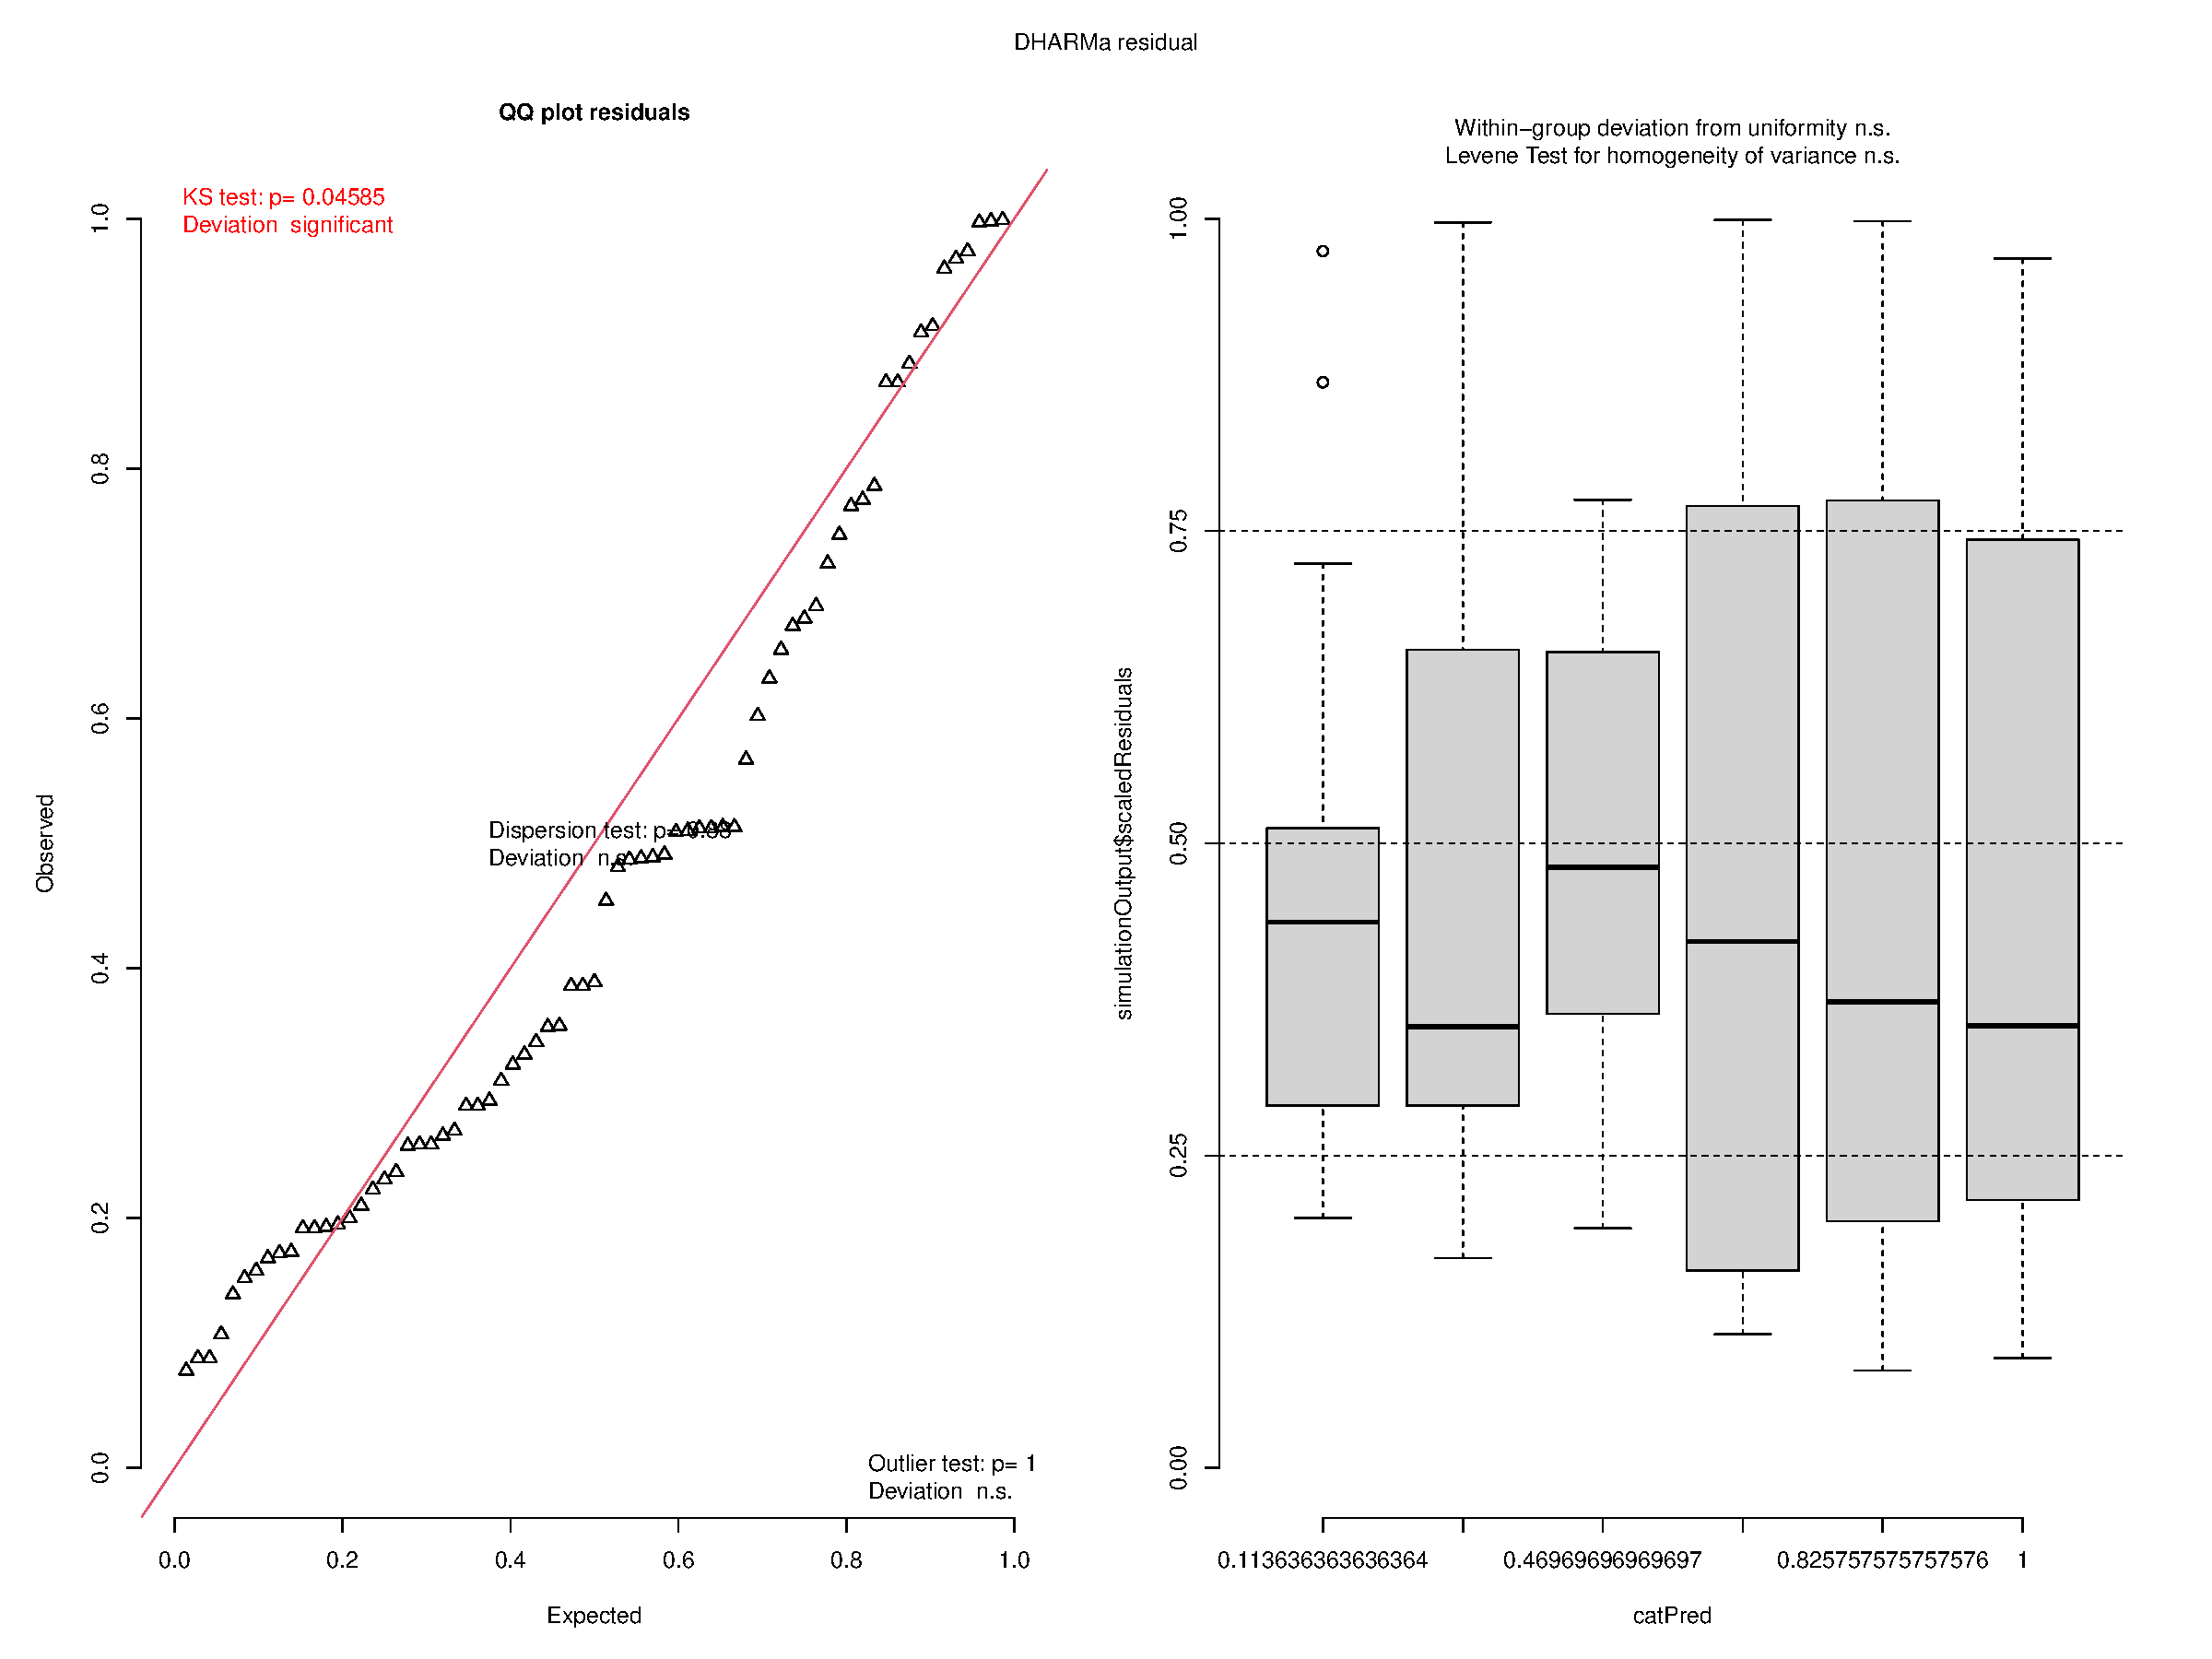
\includegraphics[keepaspectratio]{rsa_day1617_agar_files/figure-pdf/unnamed-chunk-8-2.pdf}}

\begin{Shaded}
\begin{Highlighting}[]
\FunctionTok{testUniformity}\NormalTok{(sim\_res)                     }\CommentTok{\# p \textgreater{} 0.05 = raw Gaussian fine}
\end{Highlighting}
\end{Shaded}

\pandocbounded{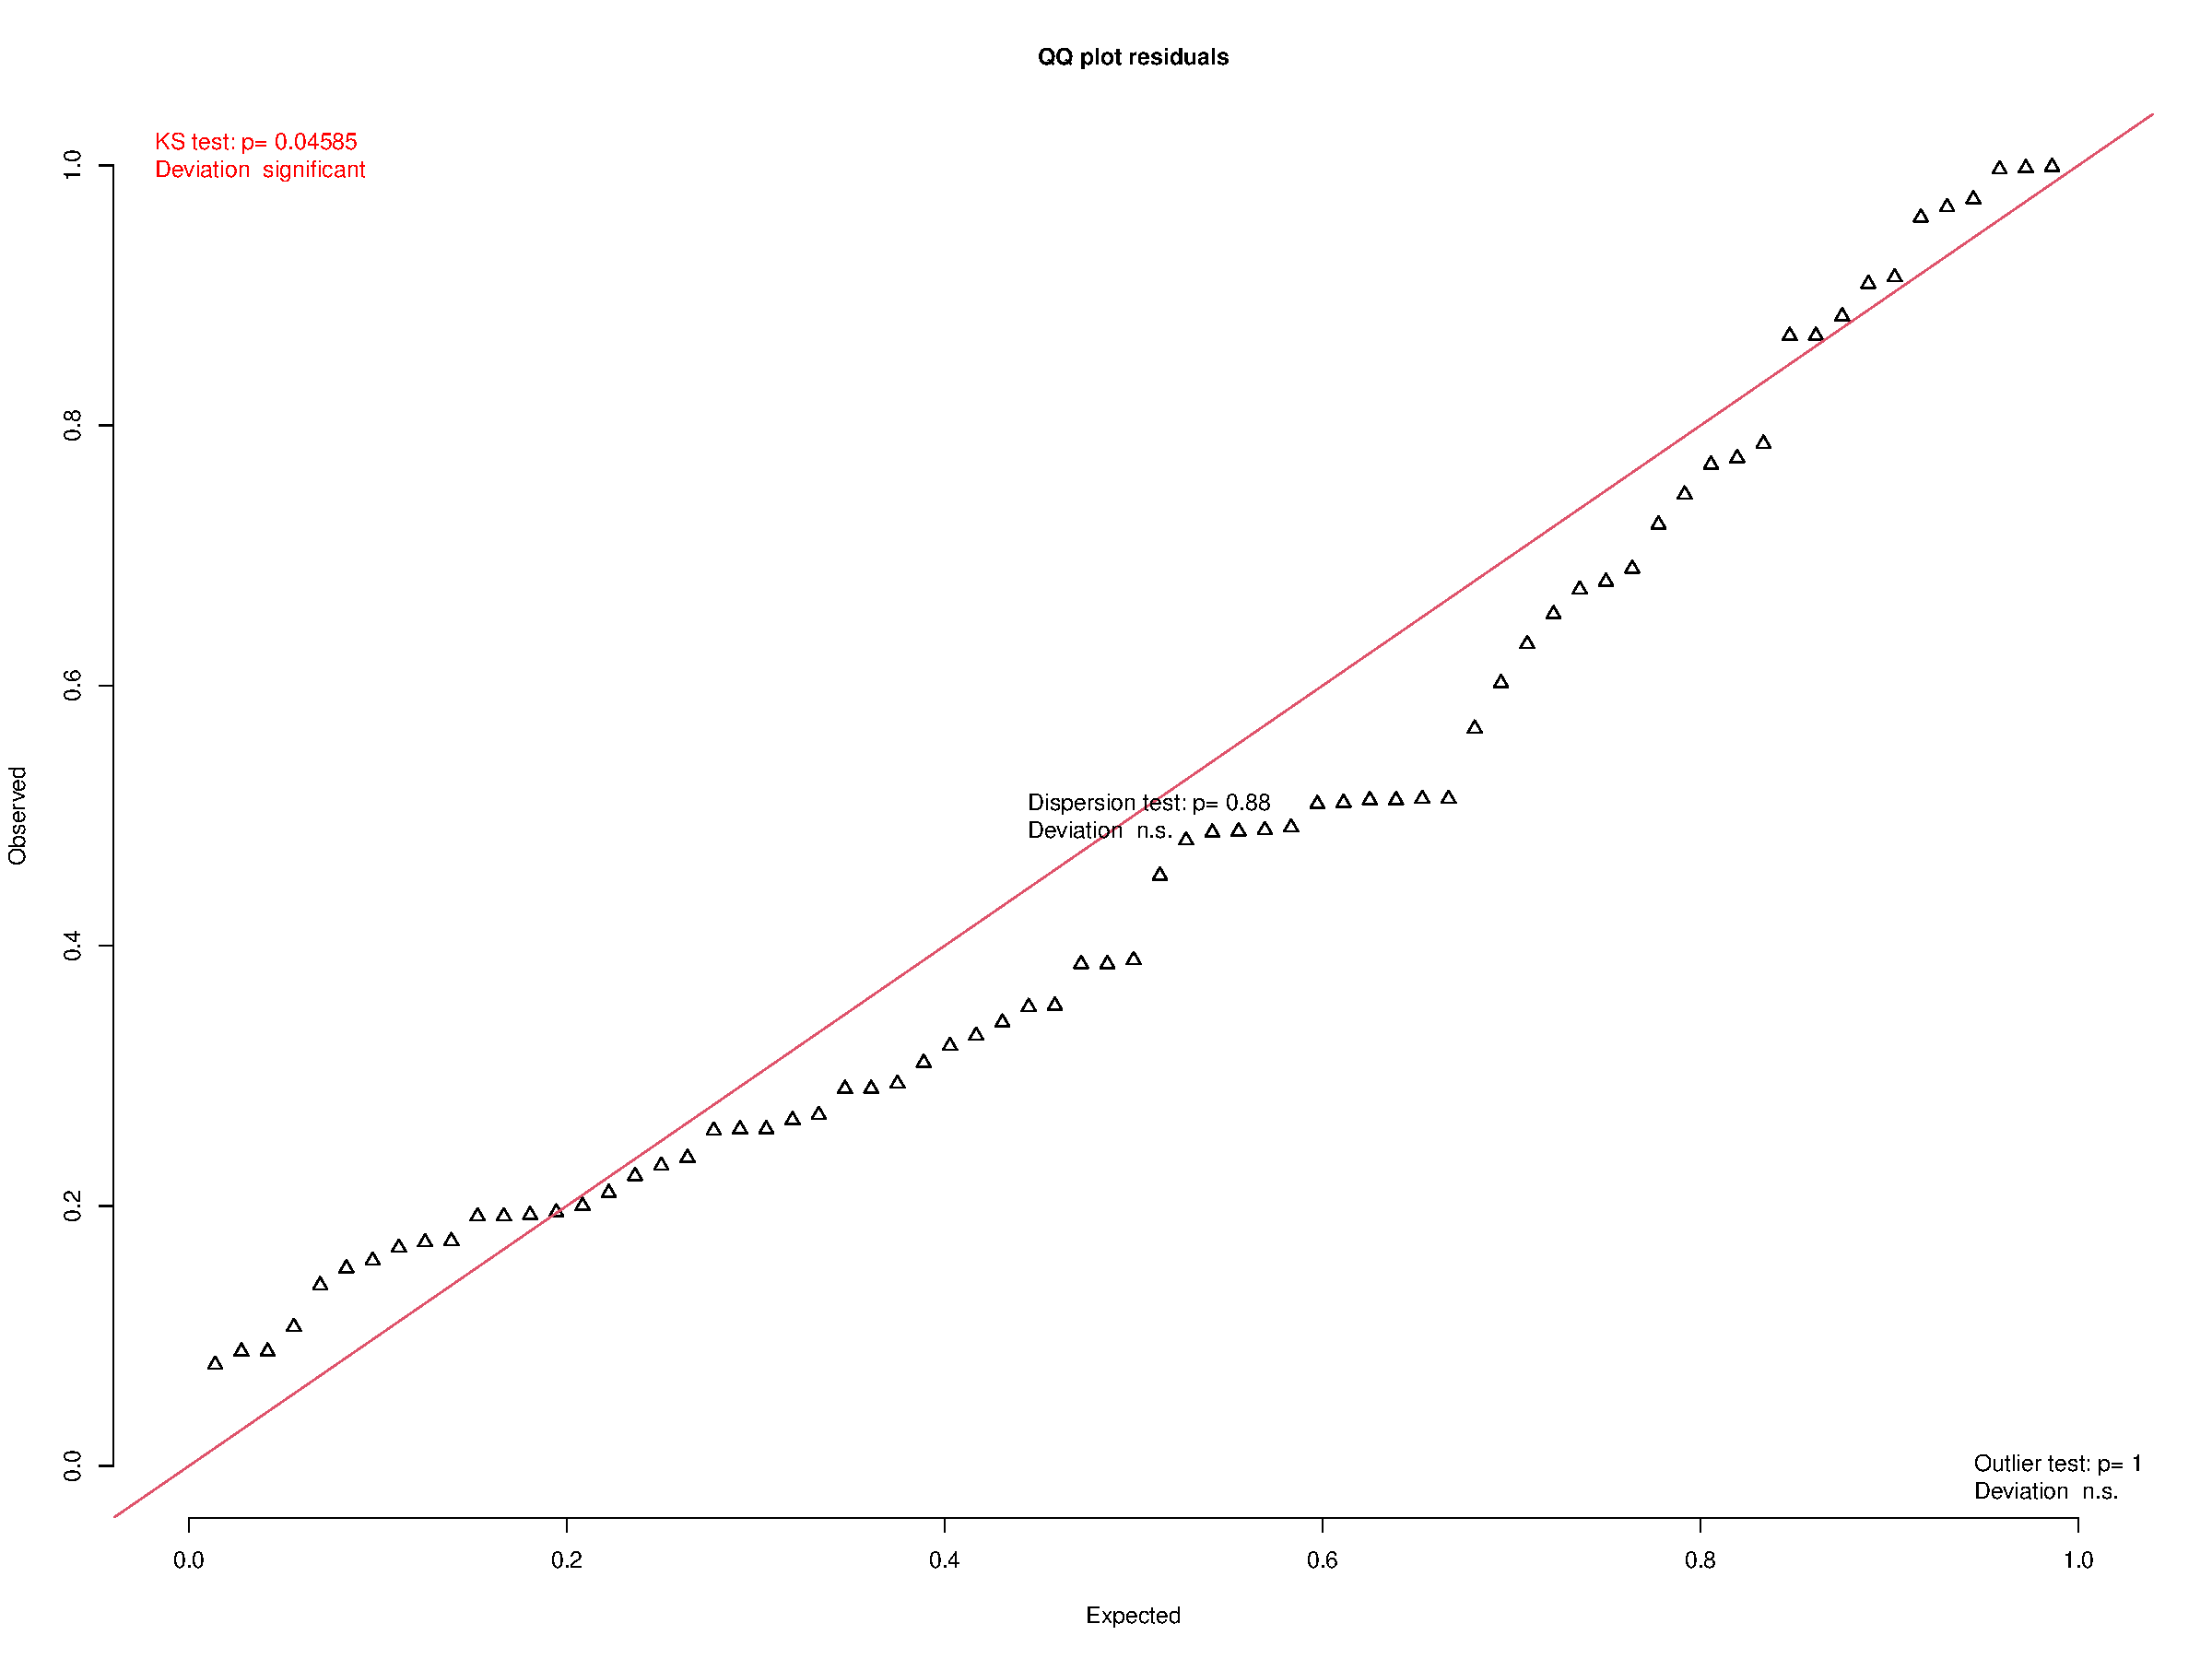
\includegraphics[keepaspectratio]{rsa_day1617_agar_files/figure-pdf/unnamed-chunk-8-3.pdf}}

\begin{verbatim}

    Asymptotic one-sample Kolmogorov-Smirnov test

data:  simulationOutput$scaledResiduals
D = 0.16306, p-value = 0.04585
alternative hypothesis: two-sided
\end{verbatim}

\begin{Shaded}
\begin{Highlighting}[]
\FunctionTok{testDispersion}\NormalTok{(sim\_res)                     }\CommentTok{\# ratio ≈ 1.0}
\end{Highlighting}
\end{Shaded}

\pandocbounded{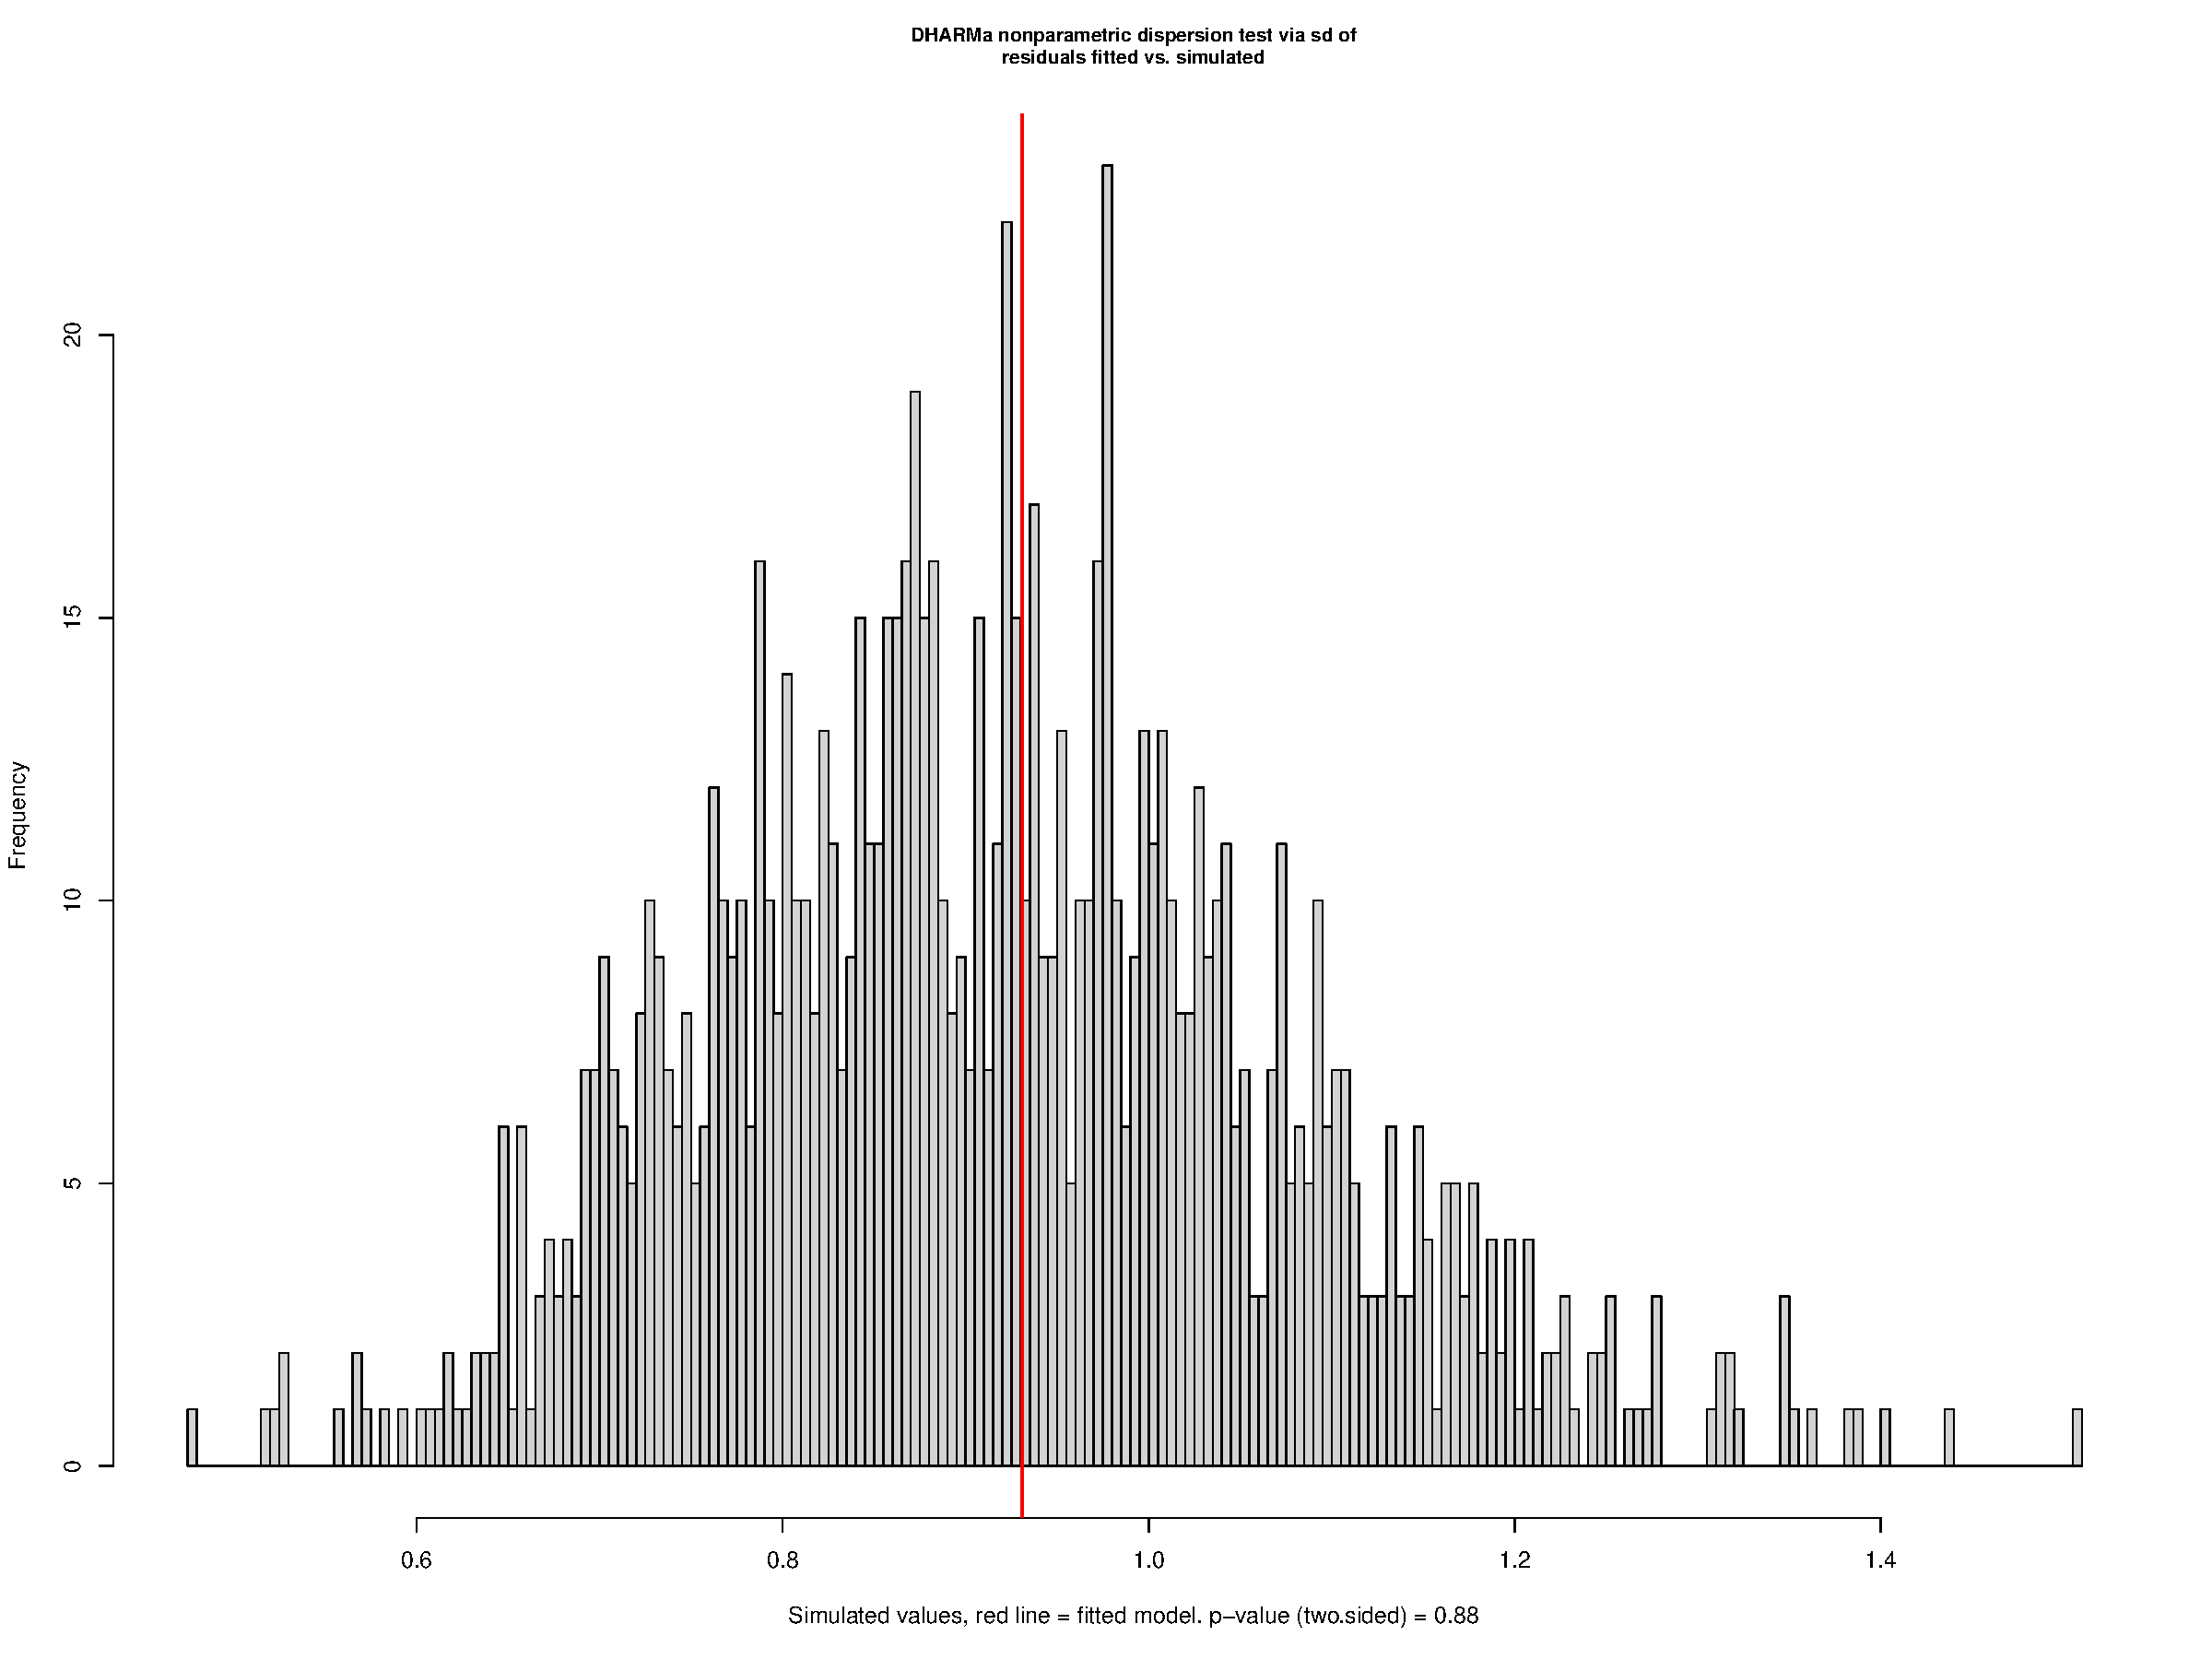
\includegraphics[keepaspectratio]{rsa_day1617_agar_files/figure-pdf/unnamed-chunk-8-4.pdf}}

\begin{verbatim}

    DHARMa nonparametric dispersion test via sd of residuals fitted vs.
    simulated

data:  simulationOutput
dispersion = 1.0146, p-value = 0.88
alternative hypothesis: two.sided
\end{verbatim}

\begin{Shaded}
\begin{Highlighting}[]
\FunctionTok{plotResiduals}\NormalTok{(sim\_res, }\AttributeTok{form =}\NormalTok{ df}\SpecialCharTok{$}\NormalTok{Genotype)  }\CommentTok{\# no patterns per genotype}
\end{Highlighting}
\end{Shaded}

\pandocbounded{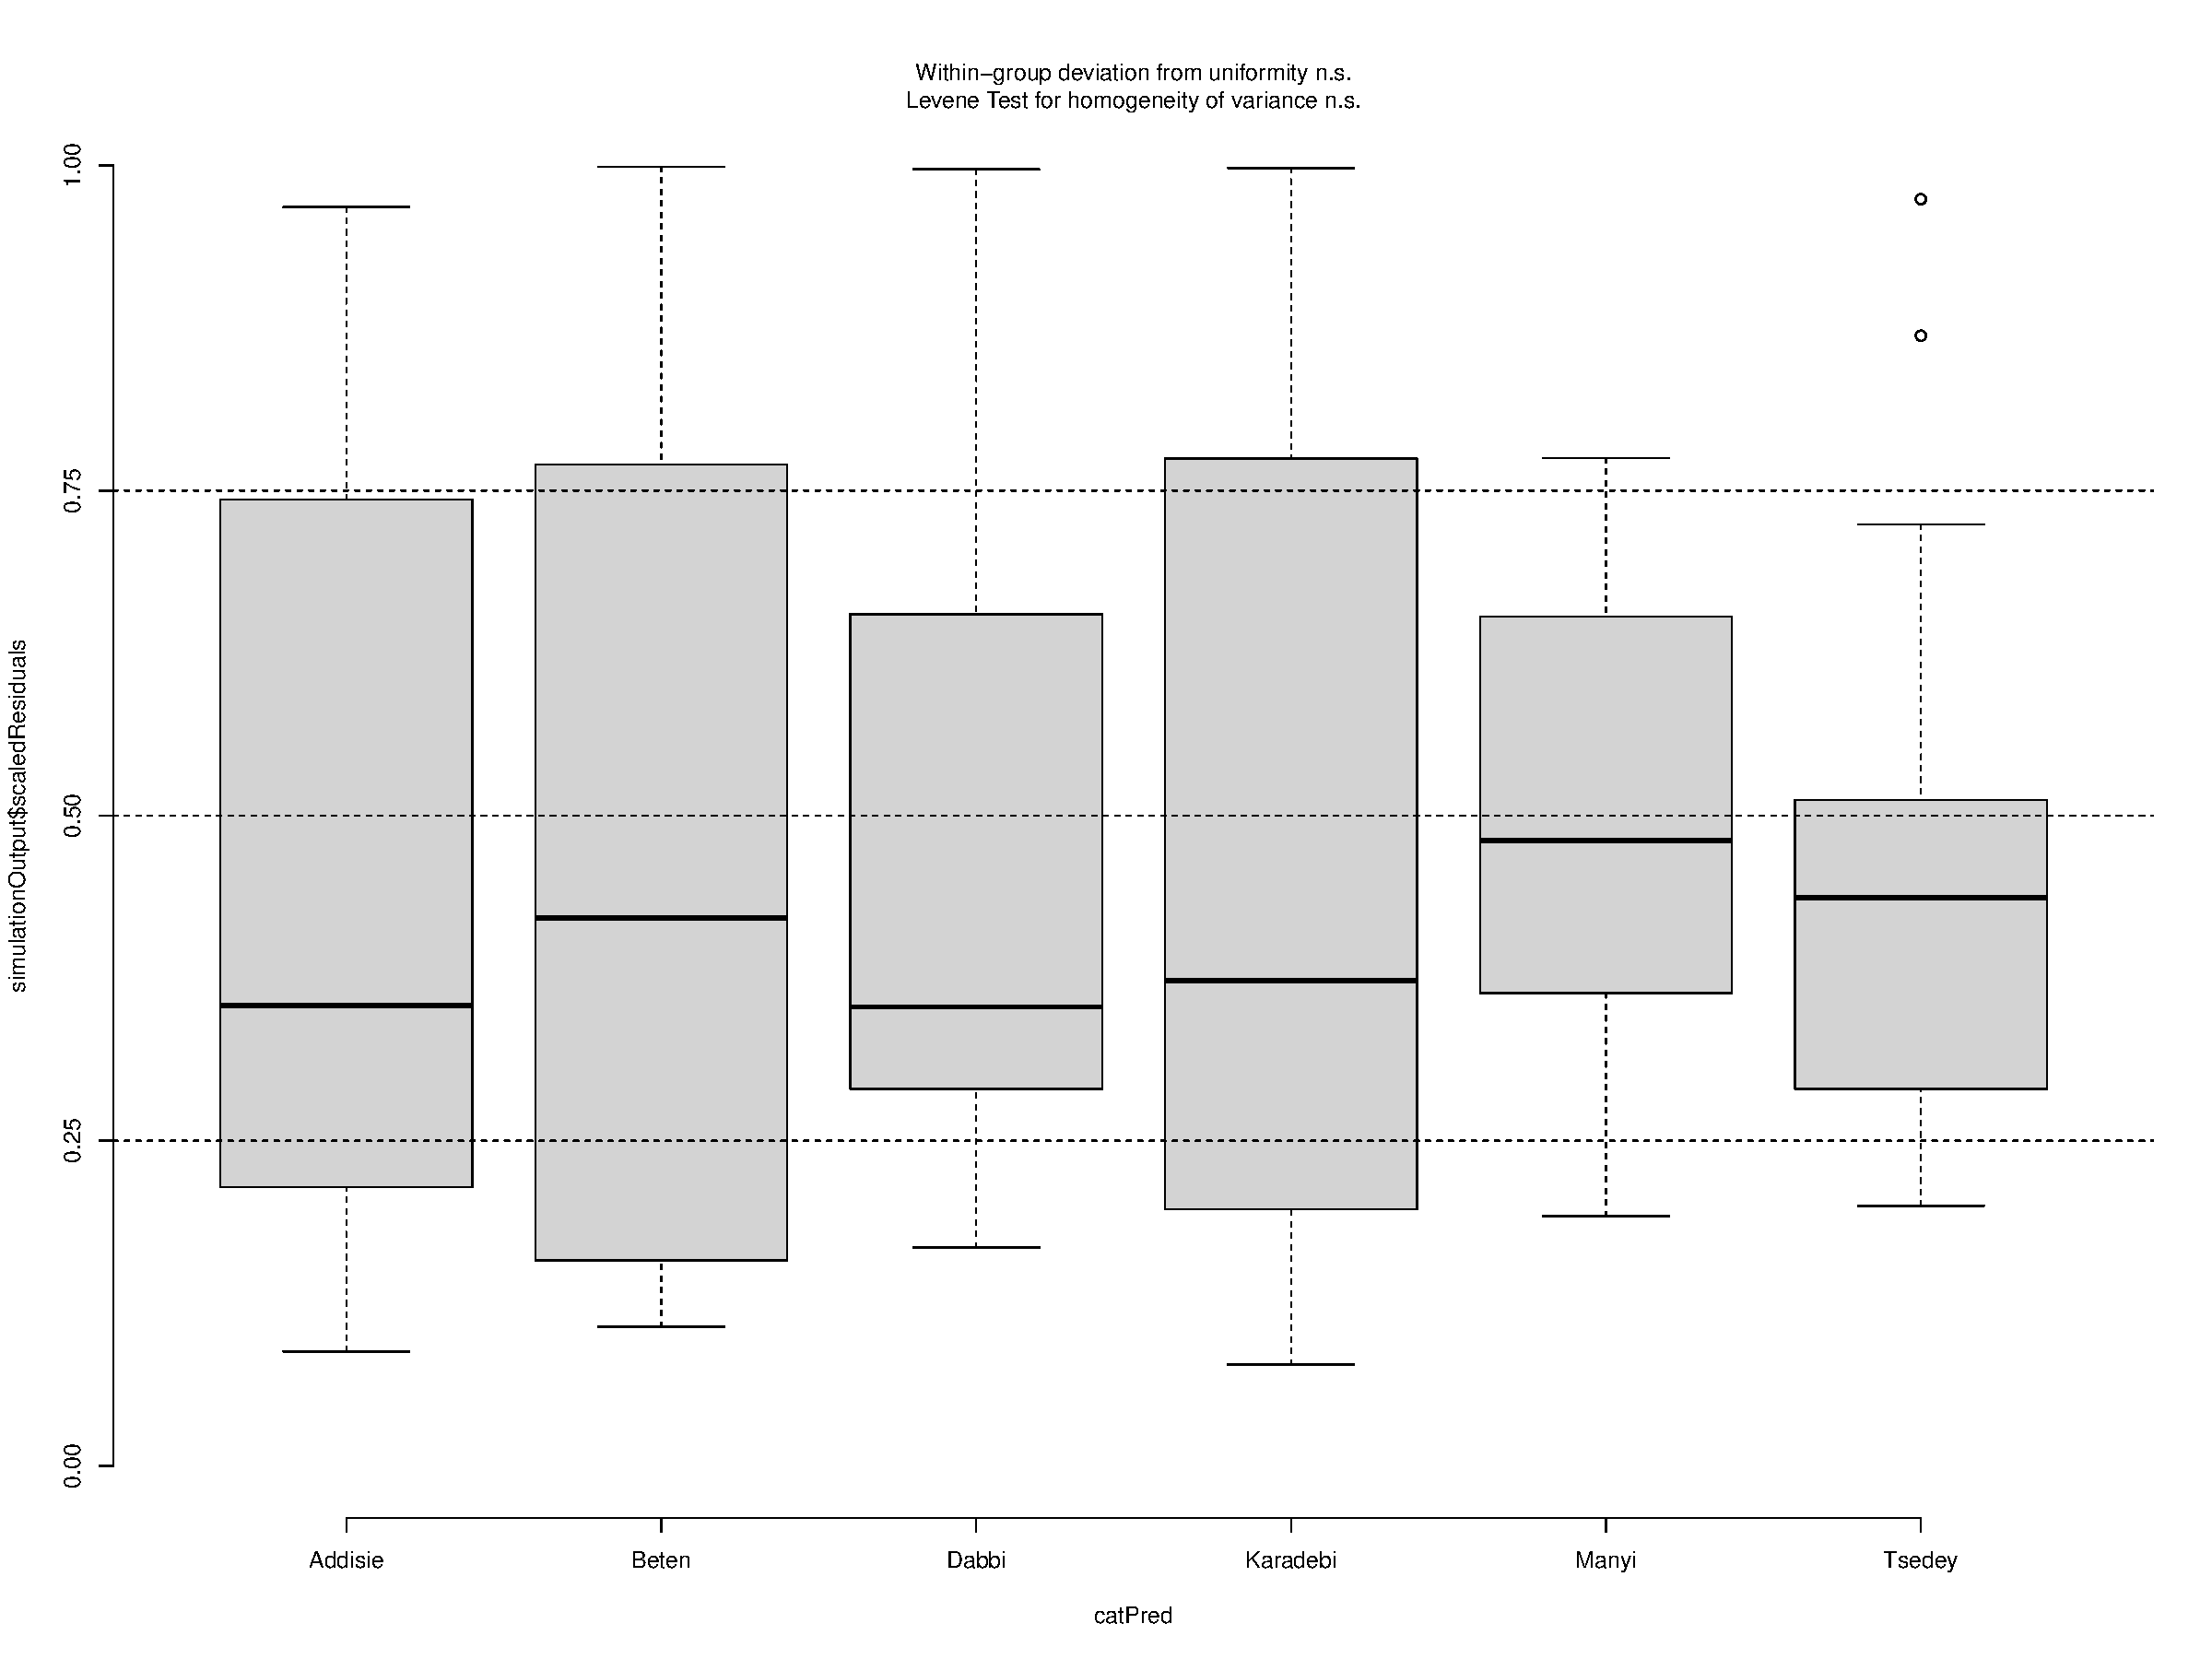
\includegraphics[keepaspectratio]{rsa_day1617_agar_files/figure-pdf/unnamed-chunk-8-5.pdf}}

\begin{Shaded}
\begin{Highlighting}[]
\CommentTok{\# singularity = true and poor model fit so trying reduced model }

\CommentTok{\# try fitting reduced model}
\NormalTok{wdr\_tmb }\OtherTok{\textless{}{-}} \FunctionTok{glmmTMB}\NormalTok{(}
  \StringTok{\textasciigrave{}}\AttributeTok{Width.to.Depth.Ratio}\StringTok{\textasciigrave{}} \SpecialCharTok{\textasciitilde{}}\NormalTok{ Genotype }\SpecialCharTok{+}\NormalTok{ (}\DecValTok{1} \SpecialCharTok{|}\NormalTok{ Batch}\SpecialCharTok{/}\NormalTok{Plate),}
  \AttributeTok{data =}\NormalTok{ df, }\AttributeTok{family =} \FunctionTok{gaussian}\NormalTok{()}
\NormalTok{)}

\FunctionTok{VarCorr}\NormalTok{(wdr\_tmb)}
\end{Highlighting}
\end{Shaded}

\begin{verbatim}

Conditional model:
 Groups      Name        Std.Dev.  
 Plate:Batch (Intercept) 4.8263e-06
 Batch       (Intercept) 2.5044e-08
 Residual                1.5393e-01
\end{verbatim}

\begin{Shaded}
\begin{Highlighting}[]
\FunctionTok{check\_singularity}\NormalTok{(wdr\_tmb)}
\end{Highlighting}
\end{Shaded}

\begin{verbatim}
[1] TRUE
\end{verbatim}

\begin{Shaded}
\begin{Highlighting}[]
\FunctionTok{summary}\NormalTok{(wdr\_tmb)}
\end{Highlighting}
\end{Shaded}

\begin{verbatim}
 Family: gaussian  ( identity )
Formula:          Width.to.Depth.Ratio ~ Genotype + (1 | Batch/Plate)
Data: df

      AIC       BIC    logLik -2*log(L)  df.resid 
    -46.2     -25.9      32.1     -64.2        62 

Random effects:

Conditional model:
 Groups      Name        Variance  Std.Dev. 
 Plate:Batch (Intercept) 2.329e-11 4.826e-06
 Batch       (Intercept) 6.272e-16 2.504e-08
 Residual                2.369e-02 1.539e-01
Number of obs: 71, groups:  Plate:Batch, 18; Batch, 4

Dispersion estimate for gaussian family (sigma^2): 0.0237 

Conditional model:
                 Estimate Std. Error z value Pr(>|z|)    
(Intercept)       0.34641    0.04641   7.464 8.39e-14 ***
GenotypeBeten    -0.04901    0.06202  -0.790   0.4294    
GenotypeDabbi    -0.08217    0.06306  -1.303   0.1925    
GenotypeKaradebi -0.02795    0.06425  -0.435   0.6635    
GenotypeManyi    -0.07353    0.07442  -0.988   0.3231    
GenotypeTsedey   -0.14072    0.06202  -2.269   0.0233 *  
---
Signif. codes:  0 '***' 0.001 '**' 0.01 '*' 0.05 '.' 0.1 ' ' 1
\end{verbatim}

\begin{Shaded}
\begin{Highlighting}[]
\CommentTok{\# this model has singularity = true as the random effects are  close to zero but model fit was good and improtant to include some random effects so will continue with this model.}

\CommentTok{\# ── 4. Assumption checks ─────}
\NormalTok{sim\_res }\OtherTok{\textless{}{-}} \FunctionTok{simulateResiduals}\NormalTok{(wdr\_tmb, }\AttributeTok{n =} \DecValTok{1000}\NormalTok{)}
\FunctionTok{plot}\NormalTok{(sim\_res)                               }\CommentTok{\# QQ + residuals vs fitted}
\end{Highlighting}
\end{Shaded}

\pandocbounded{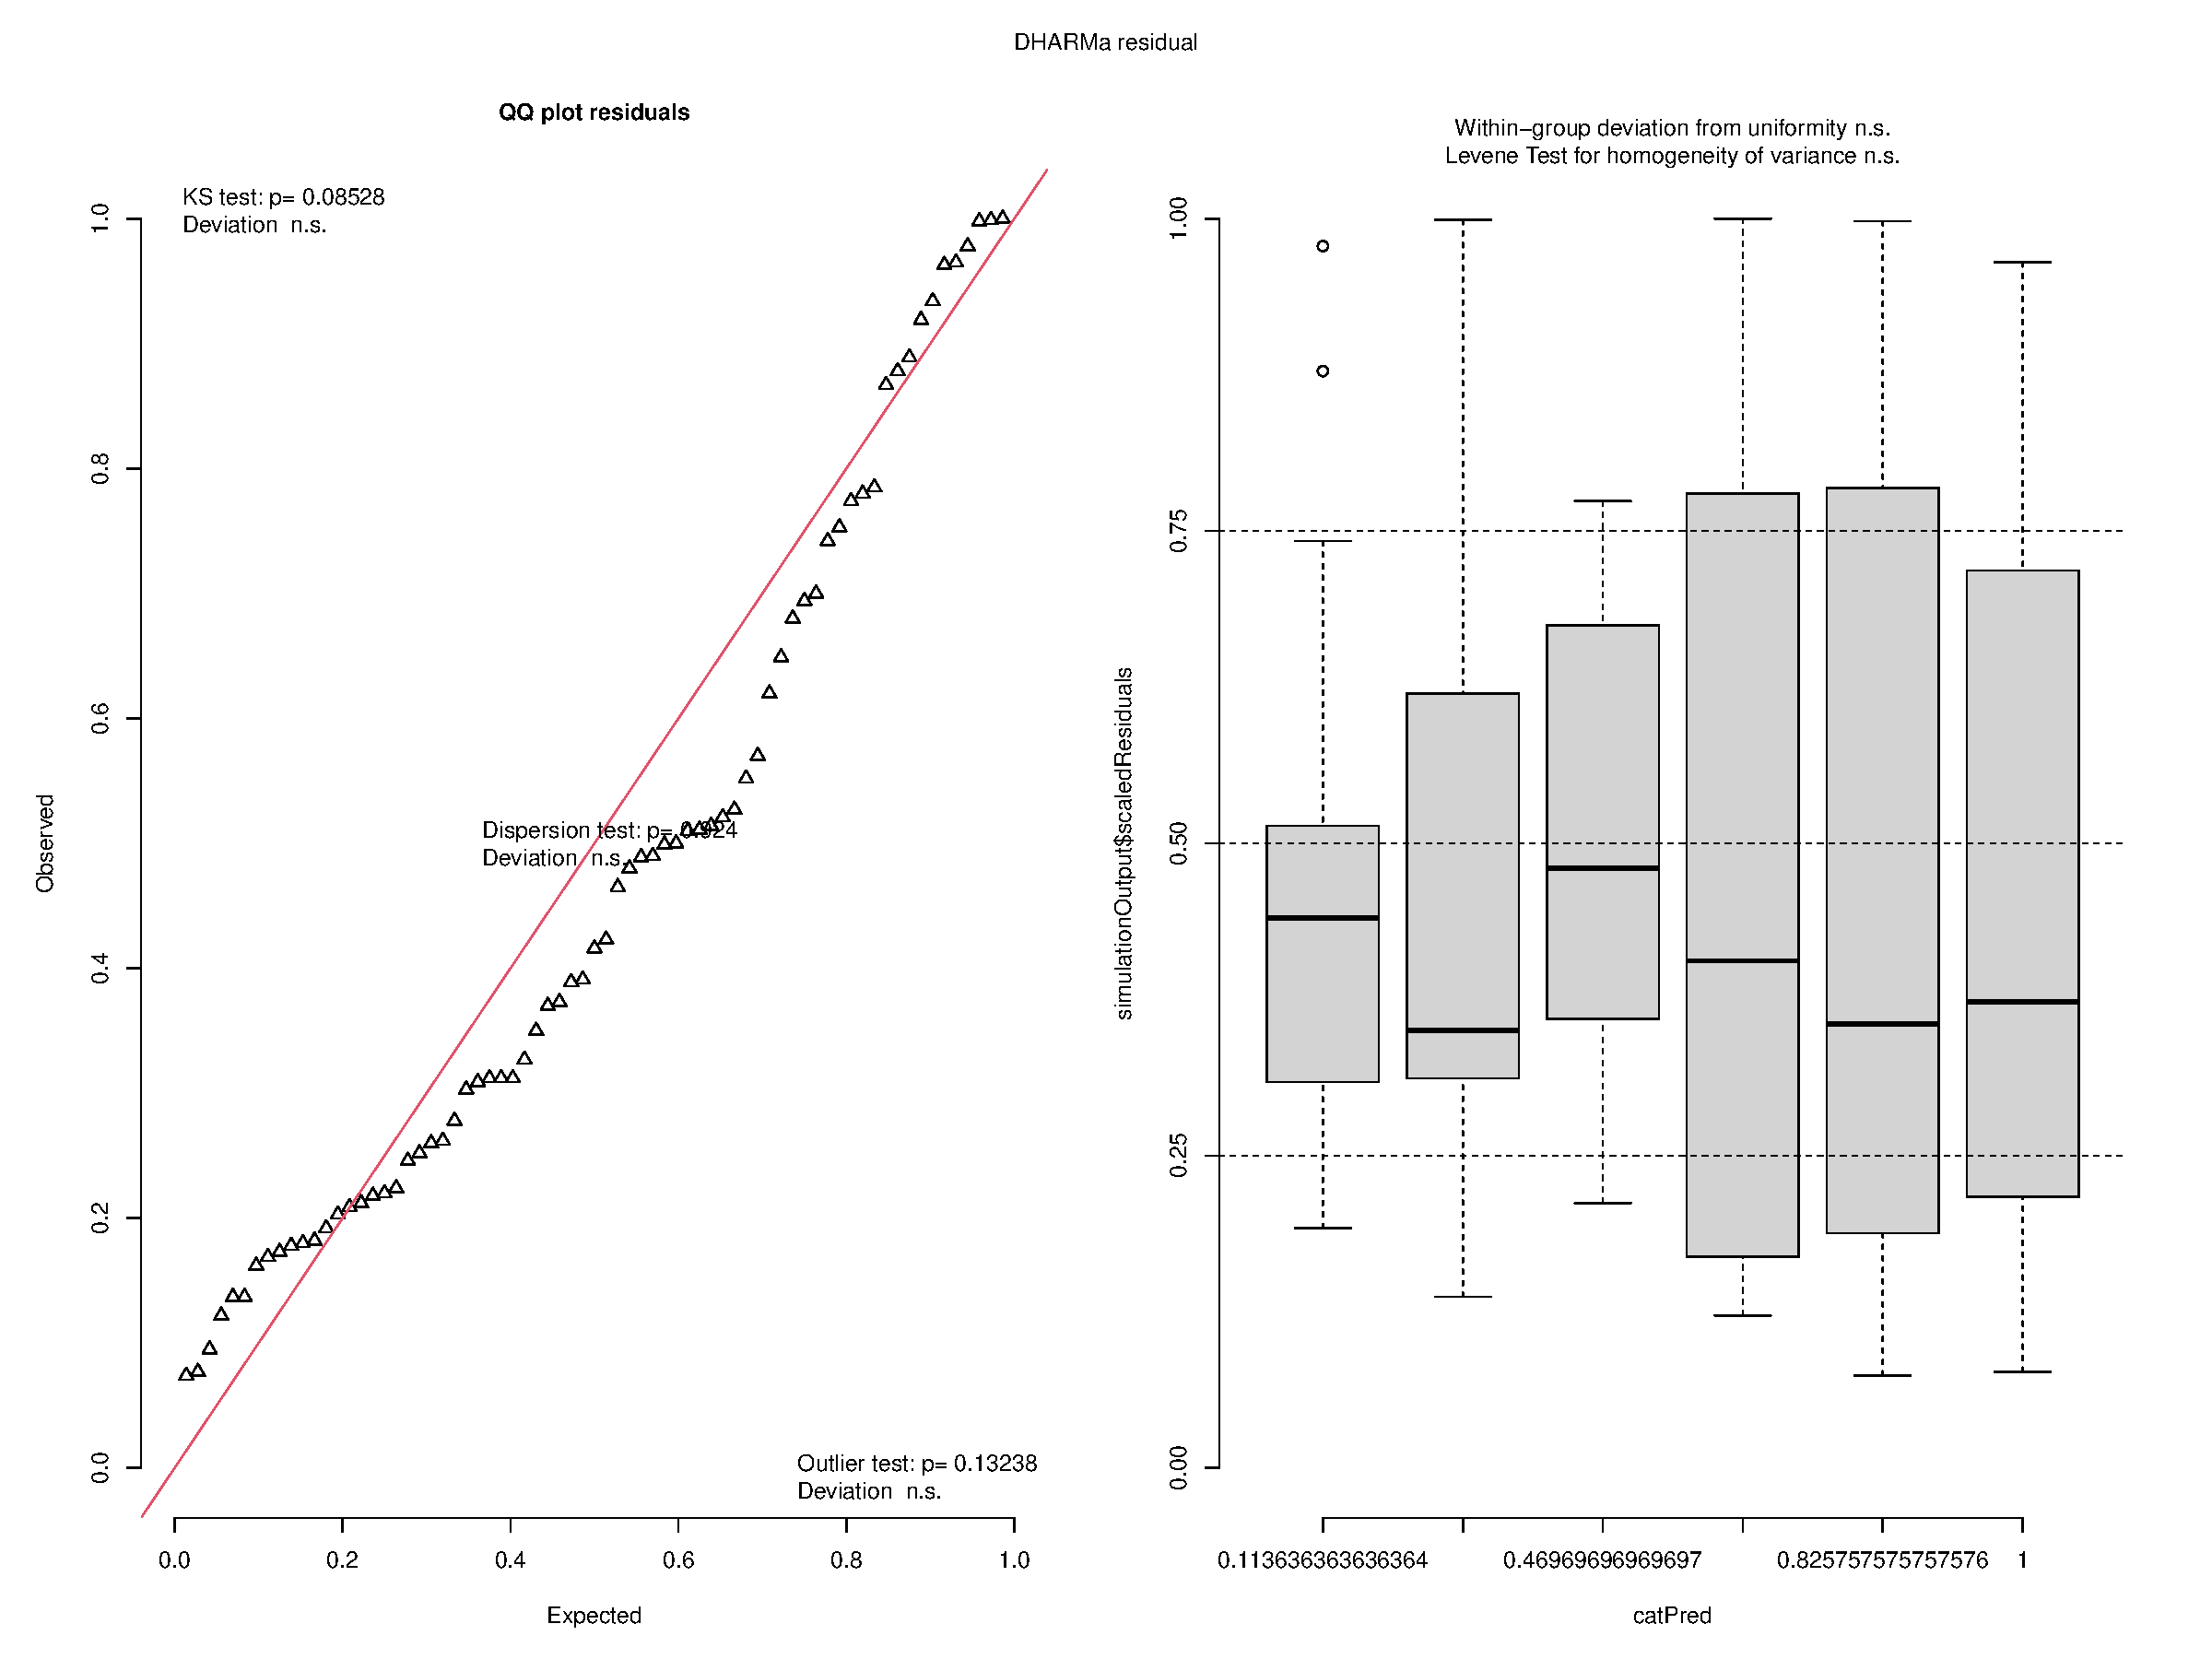
\includegraphics[keepaspectratio]{rsa_day1617_agar_files/figure-pdf/unnamed-chunk-8-6.pdf}}

\begin{Shaded}
\begin{Highlighting}[]
\FunctionTok{testUniformity}\NormalTok{(sim\_res)                     }\CommentTok{\# p \textgreater{} 0.05 = raw Gaussian fine}
\end{Highlighting}
\end{Shaded}

\pandocbounded{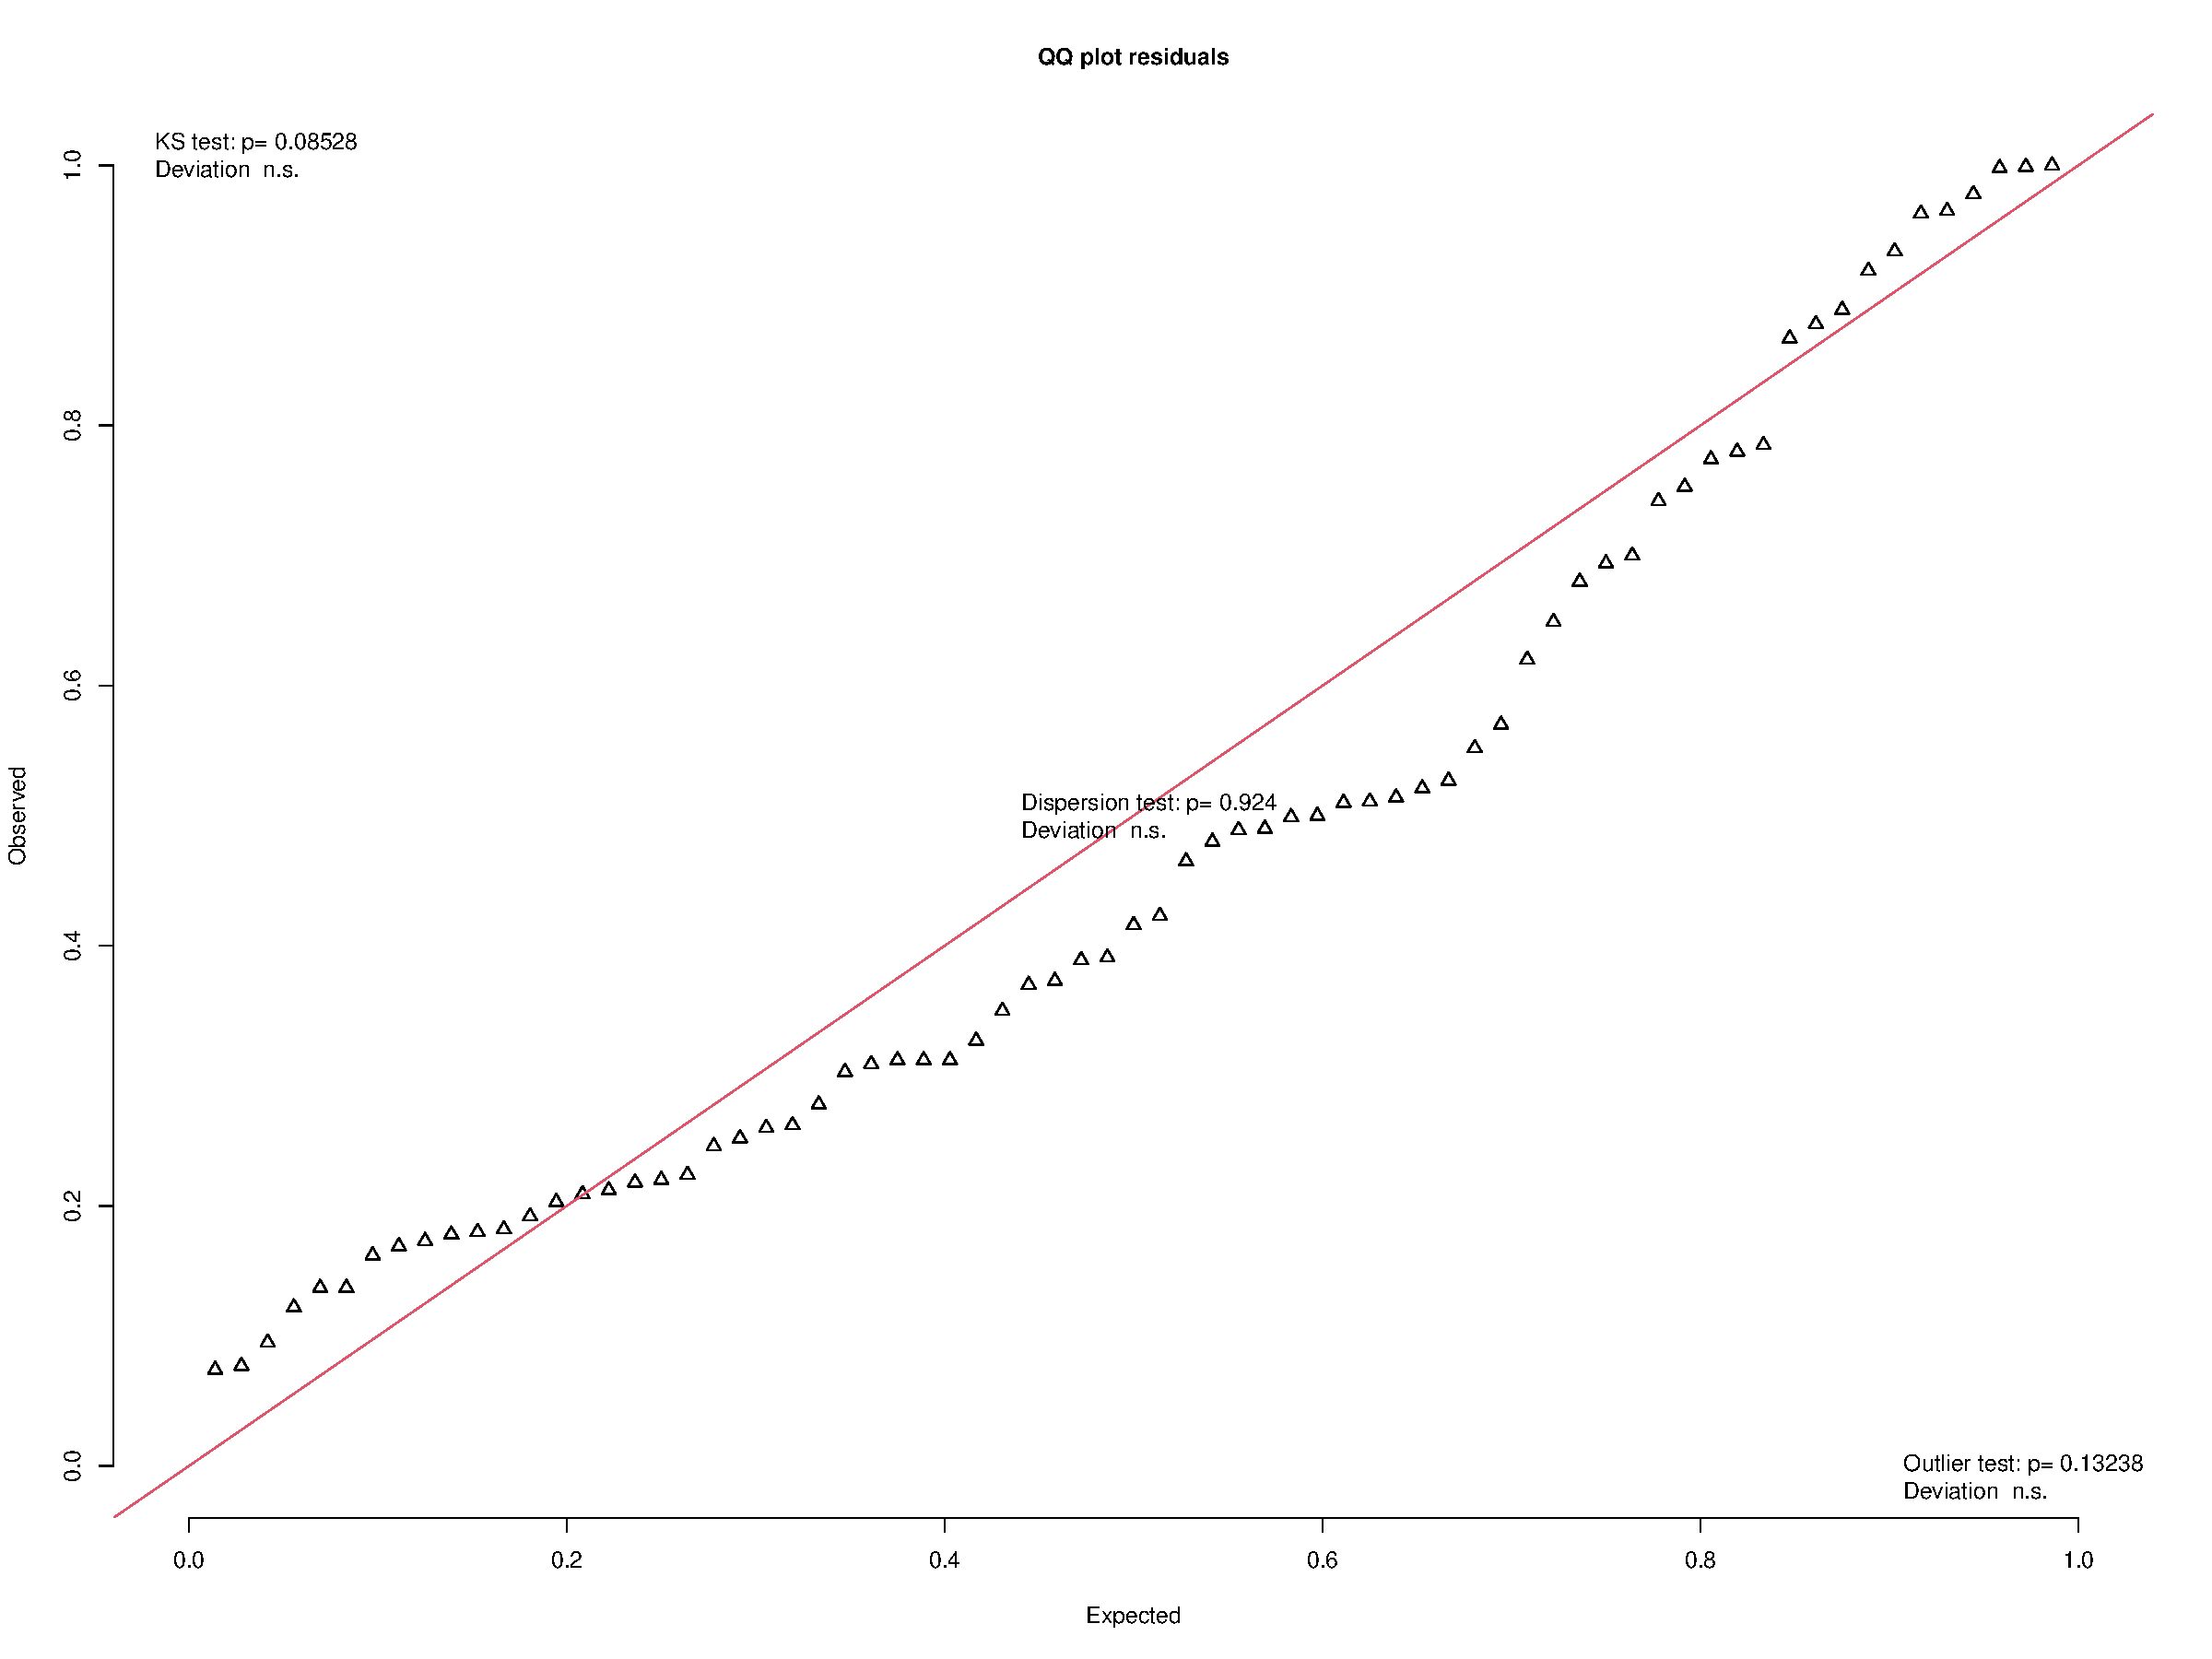
\includegraphics[keepaspectratio]{rsa_day1617_agar_files/figure-pdf/unnamed-chunk-8-7.pdf}}

\begin{verbatim}

    Asymptotic one-sample Kolmogorov-Smirnov test

data:  simulationOutput$scaledResiduals
D = 0.14906, p-value = 0.08528
alternative hypothesis: two-sided
\end{verbatim}

\begin{Shaded}
\begin{Highlighting}[]
\FunctionTok{testDispersion}\NormalTok{(sim\_res)                     }\CommentTok{\# ratio ≈ 1.0}
\end{Highlighting}
\end{Shaded}

\pandocbounded{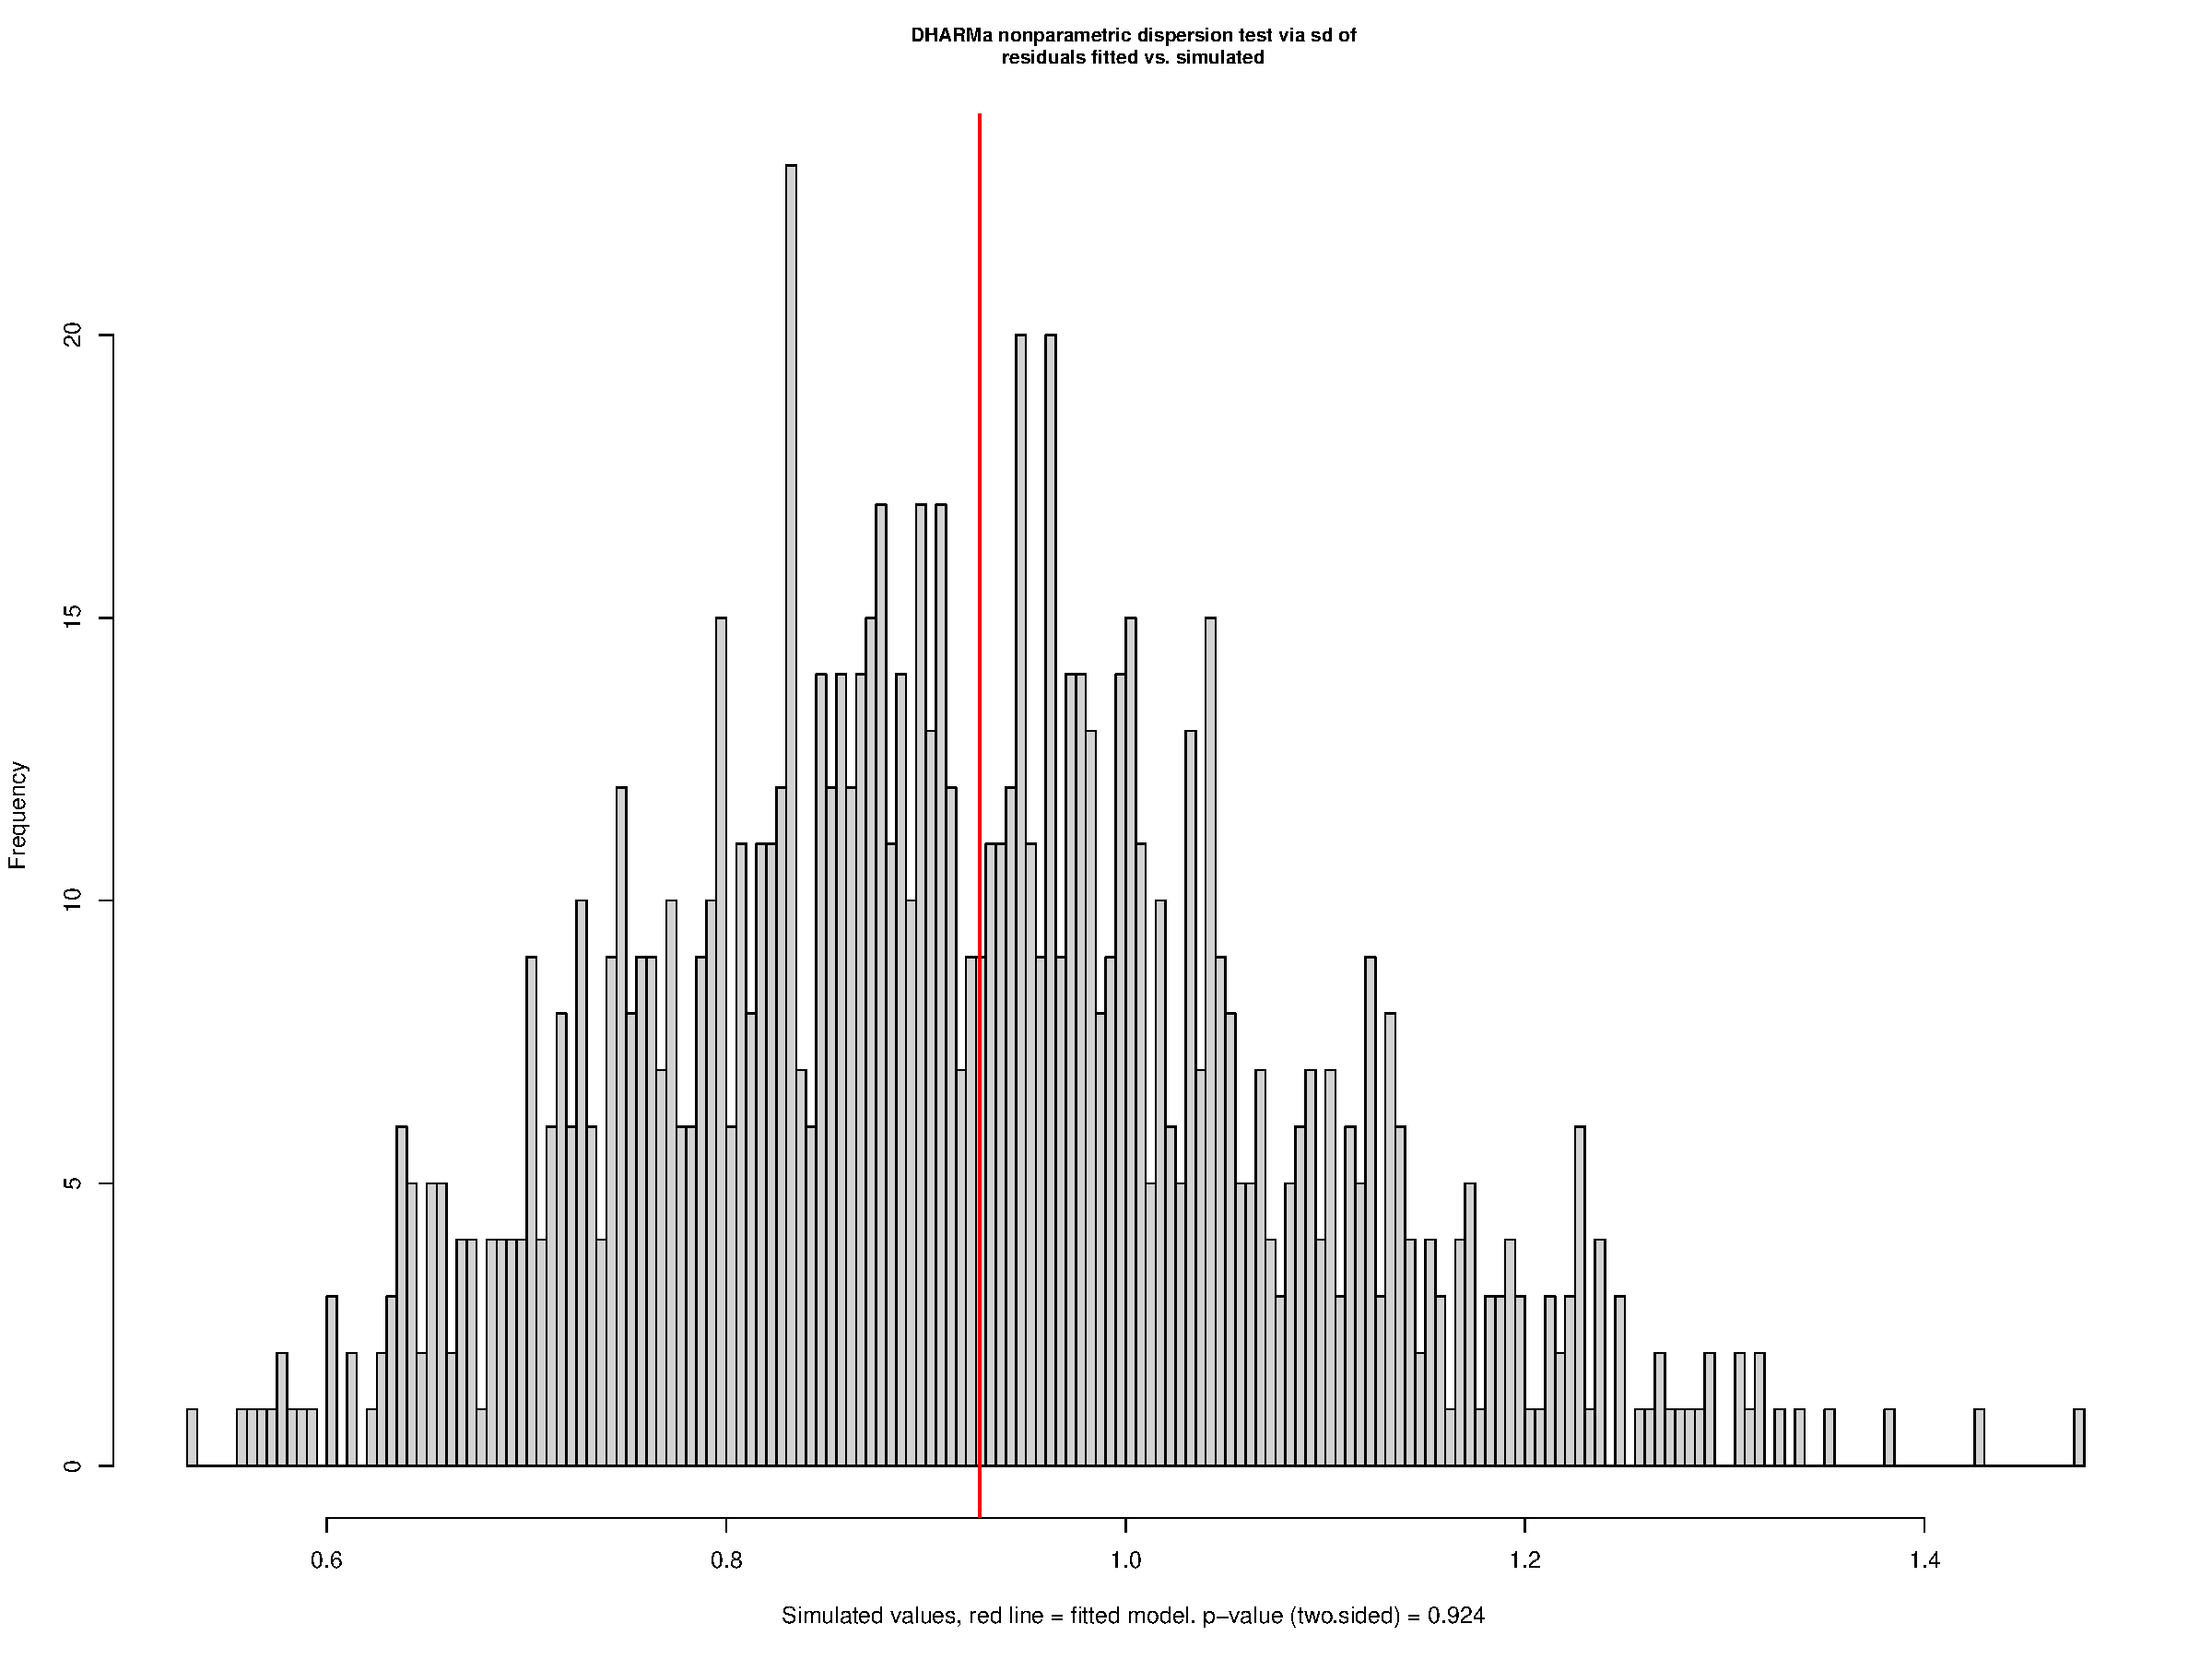
\includegraphics[keepaspectratio]{rsa_day1617_agar_files/figure-pdf/unnamed-chunk-8-8.pdf}}

\begin{verbatim}

    DHARMa nonparametric dispersion test via sd of residuals fitted vs.
    simulated

data:  simulationOutput
dispersion = 1.0104, p-value = 0.924
alternative hypothesis: two.sided
\end{verbatim}

\begin{Shaded}
\begin{Highlighting}[]
\FunctionTok{plotResiduals}\NormalTok{(sim\_res, }\AttributeTok{form =}\NormalTok{ df}\SpecialCharTok{$}\NormalTok{Genotype)  }\CommentTok{\# no patterns per genotype}
\end{Highlighting}
\end{Shaded}

\pandocbounded{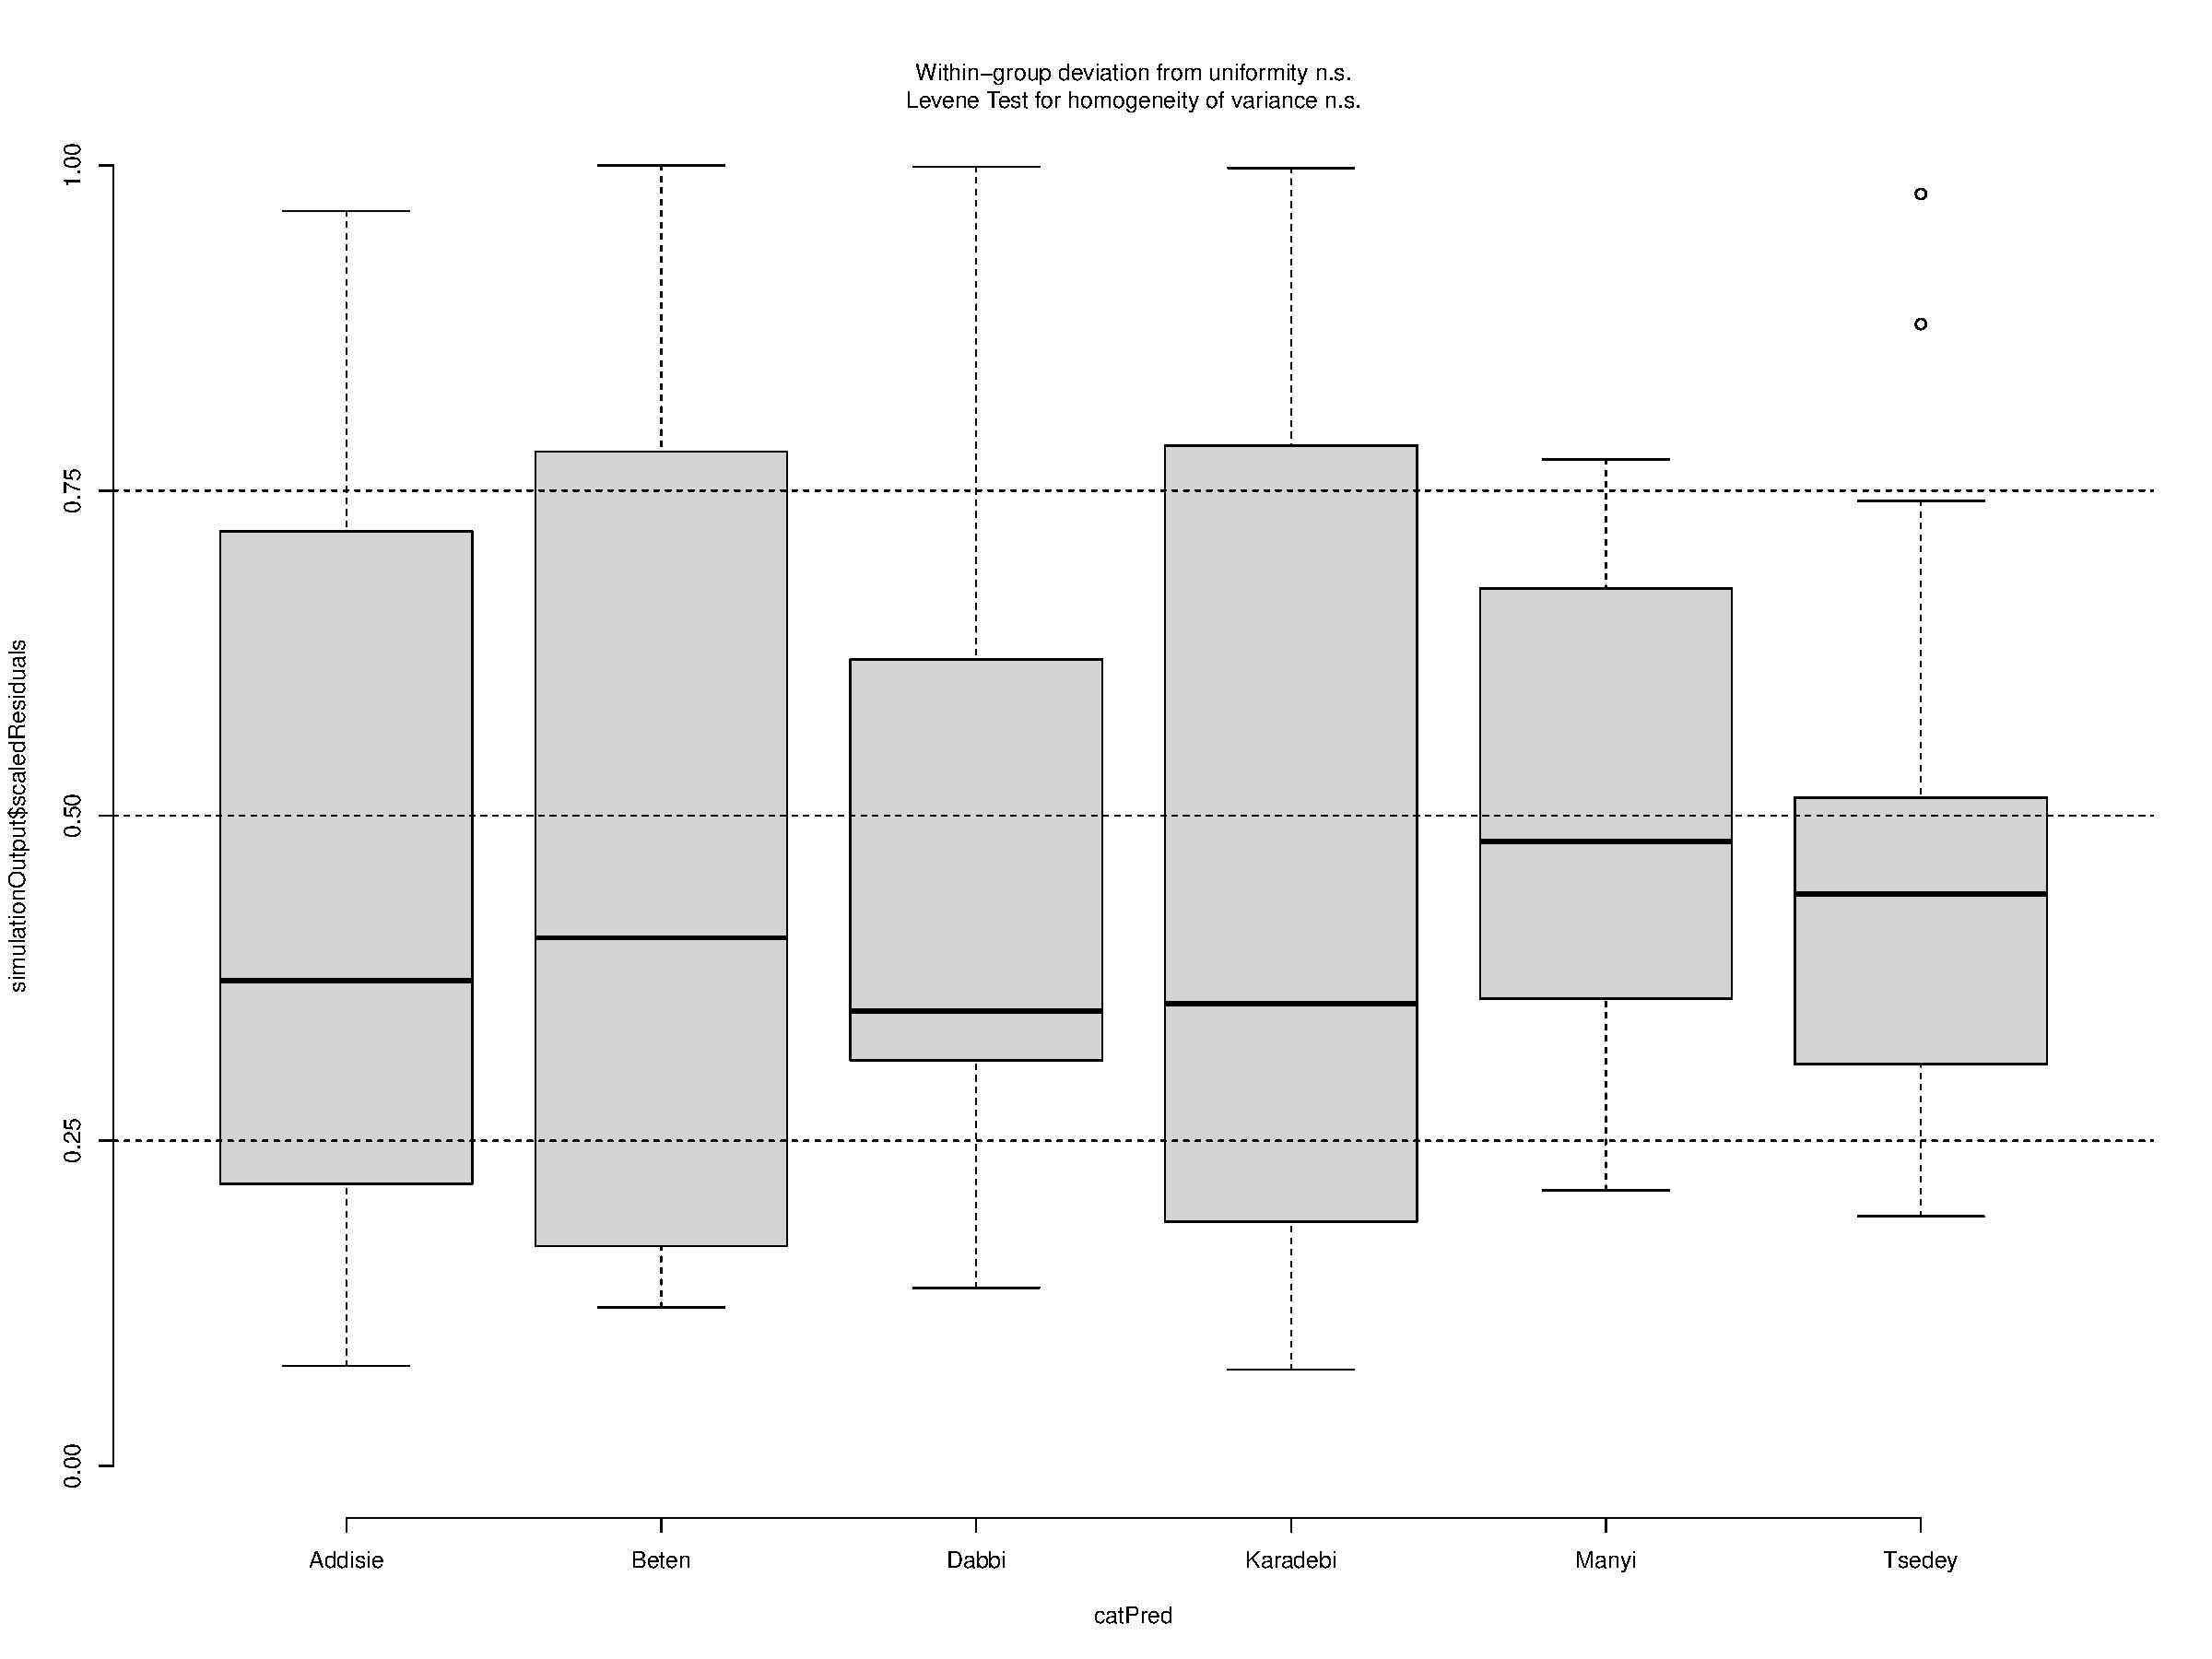
\includegraphics[keepaspectratio]{rsa_day1617_agar_files/figure-pdf/unnamed-chunk-8-9.pdf}}

\begin{Shaded}
\begin{Highlighting}[]
\CommentTok{\# ── 5. Test overall Genotype effect ──────────────────────────}
\NormalTok{car}\SpecialCharTok{::}\FunctionTok{Anova}\NormalTok{(wdr\_tmb, }\AttributeTok{type =} \StringTok{"III"}\NormalTok{)}
\end{Highlighting}
\end{Shaded}

\begin{verbatim}
Analysis of Deviance Table (Type III Wald chisquare tests)

Response: Width.to.Depth.Ratio
              Chisq Df Pr(>Chisq)    
(Intercept) 55.7132  1  8.386e-14 ***
Genotype     6.3778  5     0.2712    
---
Signif. codes:  0 '***' 0.001 '**' 0.01 '*' 0.05 '.' 0.1 ' ' 1
\end{verbatim}

\begin{Shaded}
\begin{Highlighting}[]
\CommentTok{\# ── Pairwise comparisons + CLD ────────────────────────────────}
\NormalTok{emm }\OtherTok{\textless{}{-}} \FunctionTok{emmeans}\NormalTok{(wdr\_tmb, }\SpecialCharTok{\textasciitilde{}}\NormalTok{ Genotype, }\AttributeTok{type =} \StringTok{"response"}\NormalTok{)}
\FunctionTok{pairs}\NormalTok{(emm, }\AttributeTok{adjust =} \StringTok{"sidak"}\NormalTok{)}
\end{Highlighting}
\end{Shaded}

\begin{verbatim}
 contrast           estimate     SE  df z.ratio p.value
 Addisie - Beten     0.04901 0.0620 Inf   0.790  0.9998
 Addisie - Dabbi     0.08217 0.0631 Inf   1.303  0.9596
 Addisie - Karadebi  0.02795 0.0643 Inf   0.435  1.0000
 Addisie - Manyi     0.07353 0.0744 Inf   0.988  0.9971
 Addisie - Tsedey    0.14072 0.0620 Inf   2.269  0.2976
 Beten - Dabbi       0.03317 0.0593 Inf   0.559  1.0000
 Beten - Karadebi   -0.02105 0.0606 Inf  -0.348  1.0000
 Beten - Manyi       0.02452 0.0713 Inf   0.344  1.0000
 Beten - Tsedey      0.09171 0.0582 Inf   1.576  0.8398
 Dabbi - Karadebi   -0.05422 0.0616 Inf  -0.880  0.9992
 Dabbi - Manyi      -0.00864 0.0722 Inf  -0.120  1.0000
 Dabbi - Tsedey      0.05854 0.0593 Inf   0.987  0.9972
 Karadebi - Manyi    0.04558 0.0732 Inf   0.623  1.0000
 Karadebi - Tsedey   0.11276 0.0606 Inf   1.862  0.6206
 Manyi - Tsedey      0.06719 0.0713 Inf   0.943  0.9983

P value adjustment: sidak method for 15 tests 
\end{verbatim}

\begin{Shaded}
\begin{Highlighting}[]
\NormalTok{cld\_df }\OtherTok{\textless{}{-}} \FunctionTok{as.data.frame}\NormalTok{(}\FunctionTok{cld}\NormalTok{(emm, }\AttributeTok{adjust =} \StringTok{"sidak"}\NormalTok{,}
                             \AttributeTok{Letters =}\NormalTok{ letters, }\AttributeTok{alpha =} \FloatTok{0.05}\NormalTok{)) }\SpecialCharTok{\%\textgreater{}\%}
  \FunctionTok{mutate}\NormalTok{(}\AttributeTok{.group =} \FunctionTok{trimws}\NormalTok{(.group))}

\NormalTok{n\_df }\OtherTok{\textless{}{-}}\NormalTok{ df }\SpecialCharTok{\%\textgreater{}\%}
  \FunctionTok{count}\NormalTok{(Genotype) }\SpecialCharTok{\%\textgreater{}\%}
  \FunctionTok{mutate}\NormalTok{(}\AttributeTok{label =} \FunctionTok{paste0}\NormalTok{(}\StringTok{"n="}\NormalTok{, n))}

\CommentTok{\# ── Plot ──────────────────────────────────────────────────────}

\NormalTok{y\_ceil }\OtherTok{\textless{}{-}} \FunctionTok{max}\NormalTok{(df}\SpecialCharTok{$}\NormalTok{Width.to.Depth.Ratio) }\SpecialCharTok{*} \FloatTok{1.22}
\NormalTok{y\_label }\OtherTok{\textless{}{-}}\NormalTok{ y\_ceil }\SpecialCharTok{*} \FloatTok{0.95}

\NormalTok{p1 }\OtherTok{\textless{}{-}} \FunctionTok{ggplot}\NormalTok{(df, }\FunctionTok{aes}\NormalTok{(}\AttributeTok{x =}\NormalTok{ Genotype, }\AttributeTok{y =}\NormalTok{ Width.to.Depth.Ratio, }\AttributeTok{fill =}\NormalTok{ Genotype)) }\SpecialCharTok{+}

  \FunctionTok{geom\_boxplot}\NormalTok{(}
    \AttributeTok{alpha         =} \FloatTok{0.7}\NormalTok{,}
    \AttributeTok{outlier.shape =} \ConstantTok{NA}\NormalTok{,}
    \AttributeTok{width         =} \FloatTok{0.5}\NormalTok{,}
    \AttributeTok{colour        =} \StringTok{"black"}\NormalTok{,}
    \AttributeTok{linewidth     =} \FloatTok{0.5}
\NormalTok{  ) }\SpecialCharTok{+}

  \FunctionTok{geom\_jitter}\NormalTok{(}
    \AttributeTok{width  =} \FloatTok{0.15}\NormalTok{,}
    \AttributeTok{size   =} \FloatTok{1.8}\NormalTok{,}
    \AttributeTok{alpha  =} \FloatTok{0.55}\NormalTok{,}
    \AttributeTok{colour =} \StringTok{"black"}
\NormalTok{  ) }\SpecialCharTok{+}

  \FunctionTok{geom\_text}\NormalTok{(}
    \AttributeTok{data        =}\NormalTok{ cld\_df,}
    \FunctionTok{aes}\NormalTok{(}\AttributeTok{x =}\NormalTok{ Genotype, }\AttributeTok{label =}\NormalTok{ .group),}
    \AttributeTok{y           =}\NormalTok{ y\_label,}
    \AttributeTok{inherit.aes =} \ConstantTok{FALSE}\NormalTok{,}
    \AttributeTok{size        =} \DecValTok{5}\NormalTok{,}
    \AttributeTok{fontface    =} \StringTok{"bold"}\NormalTok{,}
    \AttributeTok{colour      =} \StringTok{"grey20"}
\NormalTok{  ) }\SpecialCharTok{+}

  \FunctionTok{geom\_text}\NormalTok{(}
    \AttributeTok{data        =}\NormalTok{ n\_df,}
    \FunctionTok{aes}\NormalTok{(}\AttributeTok{x =}\NormalTok{ Genotype, }\AttributeTok{label =}\NormalTok{ label),}
    \AttributeTok{y           =} \SpecialCharTok{{-}}\ConstantTok{Inf}\NormalTok{,}
    \AttributeTok{vjust       =} \FloatTok{4.2}\NormalTok{,}
    \AttributeTok{inherit.aes =} \ConstantTok{FALSE}\NormalTok{,}
    \AttributeTok{size        =} \FloatTok{3.5}\NormalTok{,}
    \AttributeTok{colour      =} \StringTok{"grey40"}
\NormalTok{  ) }\SpecialCharTok{+}

  \FunctionTok{scale\_fill\_brewer}\NormalTok{(}\AttributeTok{palette =} \StringTok{"Set2"}\NormalTok{) }\SpecialCharTok{+}

  \FunctionTok{labs}\NormalTok{(}
    \AttributeTok{x       =} \StringTok{"Genotype"}\NormalTok{,}
    \AttributeTok{y       =} \StringTok{"Width{-}to{-}depth ratio"}\NormalTok{,}
    \AttributeTok{caption =} \StringTok{"Shared letters indicate no significant difference (sidak HSD, p \textgreater{} 0.05; glmmTMB, Gaussian)"}
\NormalTok{  ) }\SpecialCharTok{+}

  \FunctionTok{theme\_classic}\NormalTok{(}\AttributeTok{base\_size =} \DecValTok{14}\NormalTok{) }\SpecialCharTok{+}
  \FunctionTok{theme}\NormalTok{(}
    \AttributeTok{legend.position =} \StringTok{"none"}\NormalTok{,}
    \AttributeTok{axis.line       =} \FunctionTok{element\_line}\NormalTok{(}\AttributeTok{colour =} \StringTok{"black"}\NormalTok{, }\AttributeTok{linewidth =} \FloatTok{0.6}\NormalTok{),}
    \AttributeTok{axis.ticks      =} \FunctionTok{element\_line}\NormalTok{(}\AttributeTok{colour =} \StringTok{"black"}\NormalTok{, }\AttributeTok{linewidth =} \FloatTok{0.5}\NormalTok{),}
    \AttributeTok{axis.title      =} \FunctionTok{element\_text}\NormalTok{(}\AttributeTok{size =} \DecValTok{14}\NormalTok{, }\AttributeTok{face =} \StringTok{"bold"}\NormalTok{),}
    \AttributeTok{axis.text       =} \FunctionTok{element\_text}\NormalTok{(}\AttributeTok{size =} \DecValTok{14}\NormalTok{, }\AttributeTok{colour =} \StringTok{"black"}\NormalTok{),}
    \AttributeTok{axis.text.x     =} \FunctionTok{element\_text}\NormalTok{(}\AttributeTok{face =} \StringTok{"italic"}\NormalTok{, }\AttributeTok{margin =} \FunctionTok{margin}\NormalTok{(}\AttributeTok{t =} \DecValTok{3}\NormalTok{)),}
    \AttributeTok{plot.caption    =} \FunctionTok{element\_text}\NormalTok{(}\AttributeTok{size =} \DecValTok{9}\NormalTok{, }\AttributeTok{colour =} \StringTok{"grey40"}\NormalTok{, }\AttributeTok{hjust =} \DecValTok{0}\NormalTok{),}
    \AttributeTok{plot.margin     =} \FunctionTok{margin}\NormalTok{(}\AttributeTok{t =} \DecValTok{10}\NormalTok{, }\AttributeTok{r =} \DecValTok{15}\NormalTok{, }\AttributeTok{b =} \DecValTok{30}\NormalTok{, }\AttributeTok{l =} \DecValTok{10}\NormalTok{)}
\NormalTok{  )}

\NormalTok{p1 }\SpecialCharTok{+} \FunctionTok{coord\_cartesian}\NormalTok{(}
  \AttributeTok{ylim =} \FunctionTok{c}\NormalTok{(}\DecValTok{0}\NormalTok{, }\FunctionTok{max}\NormalTok{(df}\SpecialCharTok{$}\NormalTok{Width.to.Depth.Ratio) }\SpecialCharTok{*} \FloatTok{1.22}\NormalTok{),}
  \AttributeTok{clip =} \StringTok{"off"}
\NormalTok{)}
\end{Highlighting}
\end{Shaded}

\pandocbounded{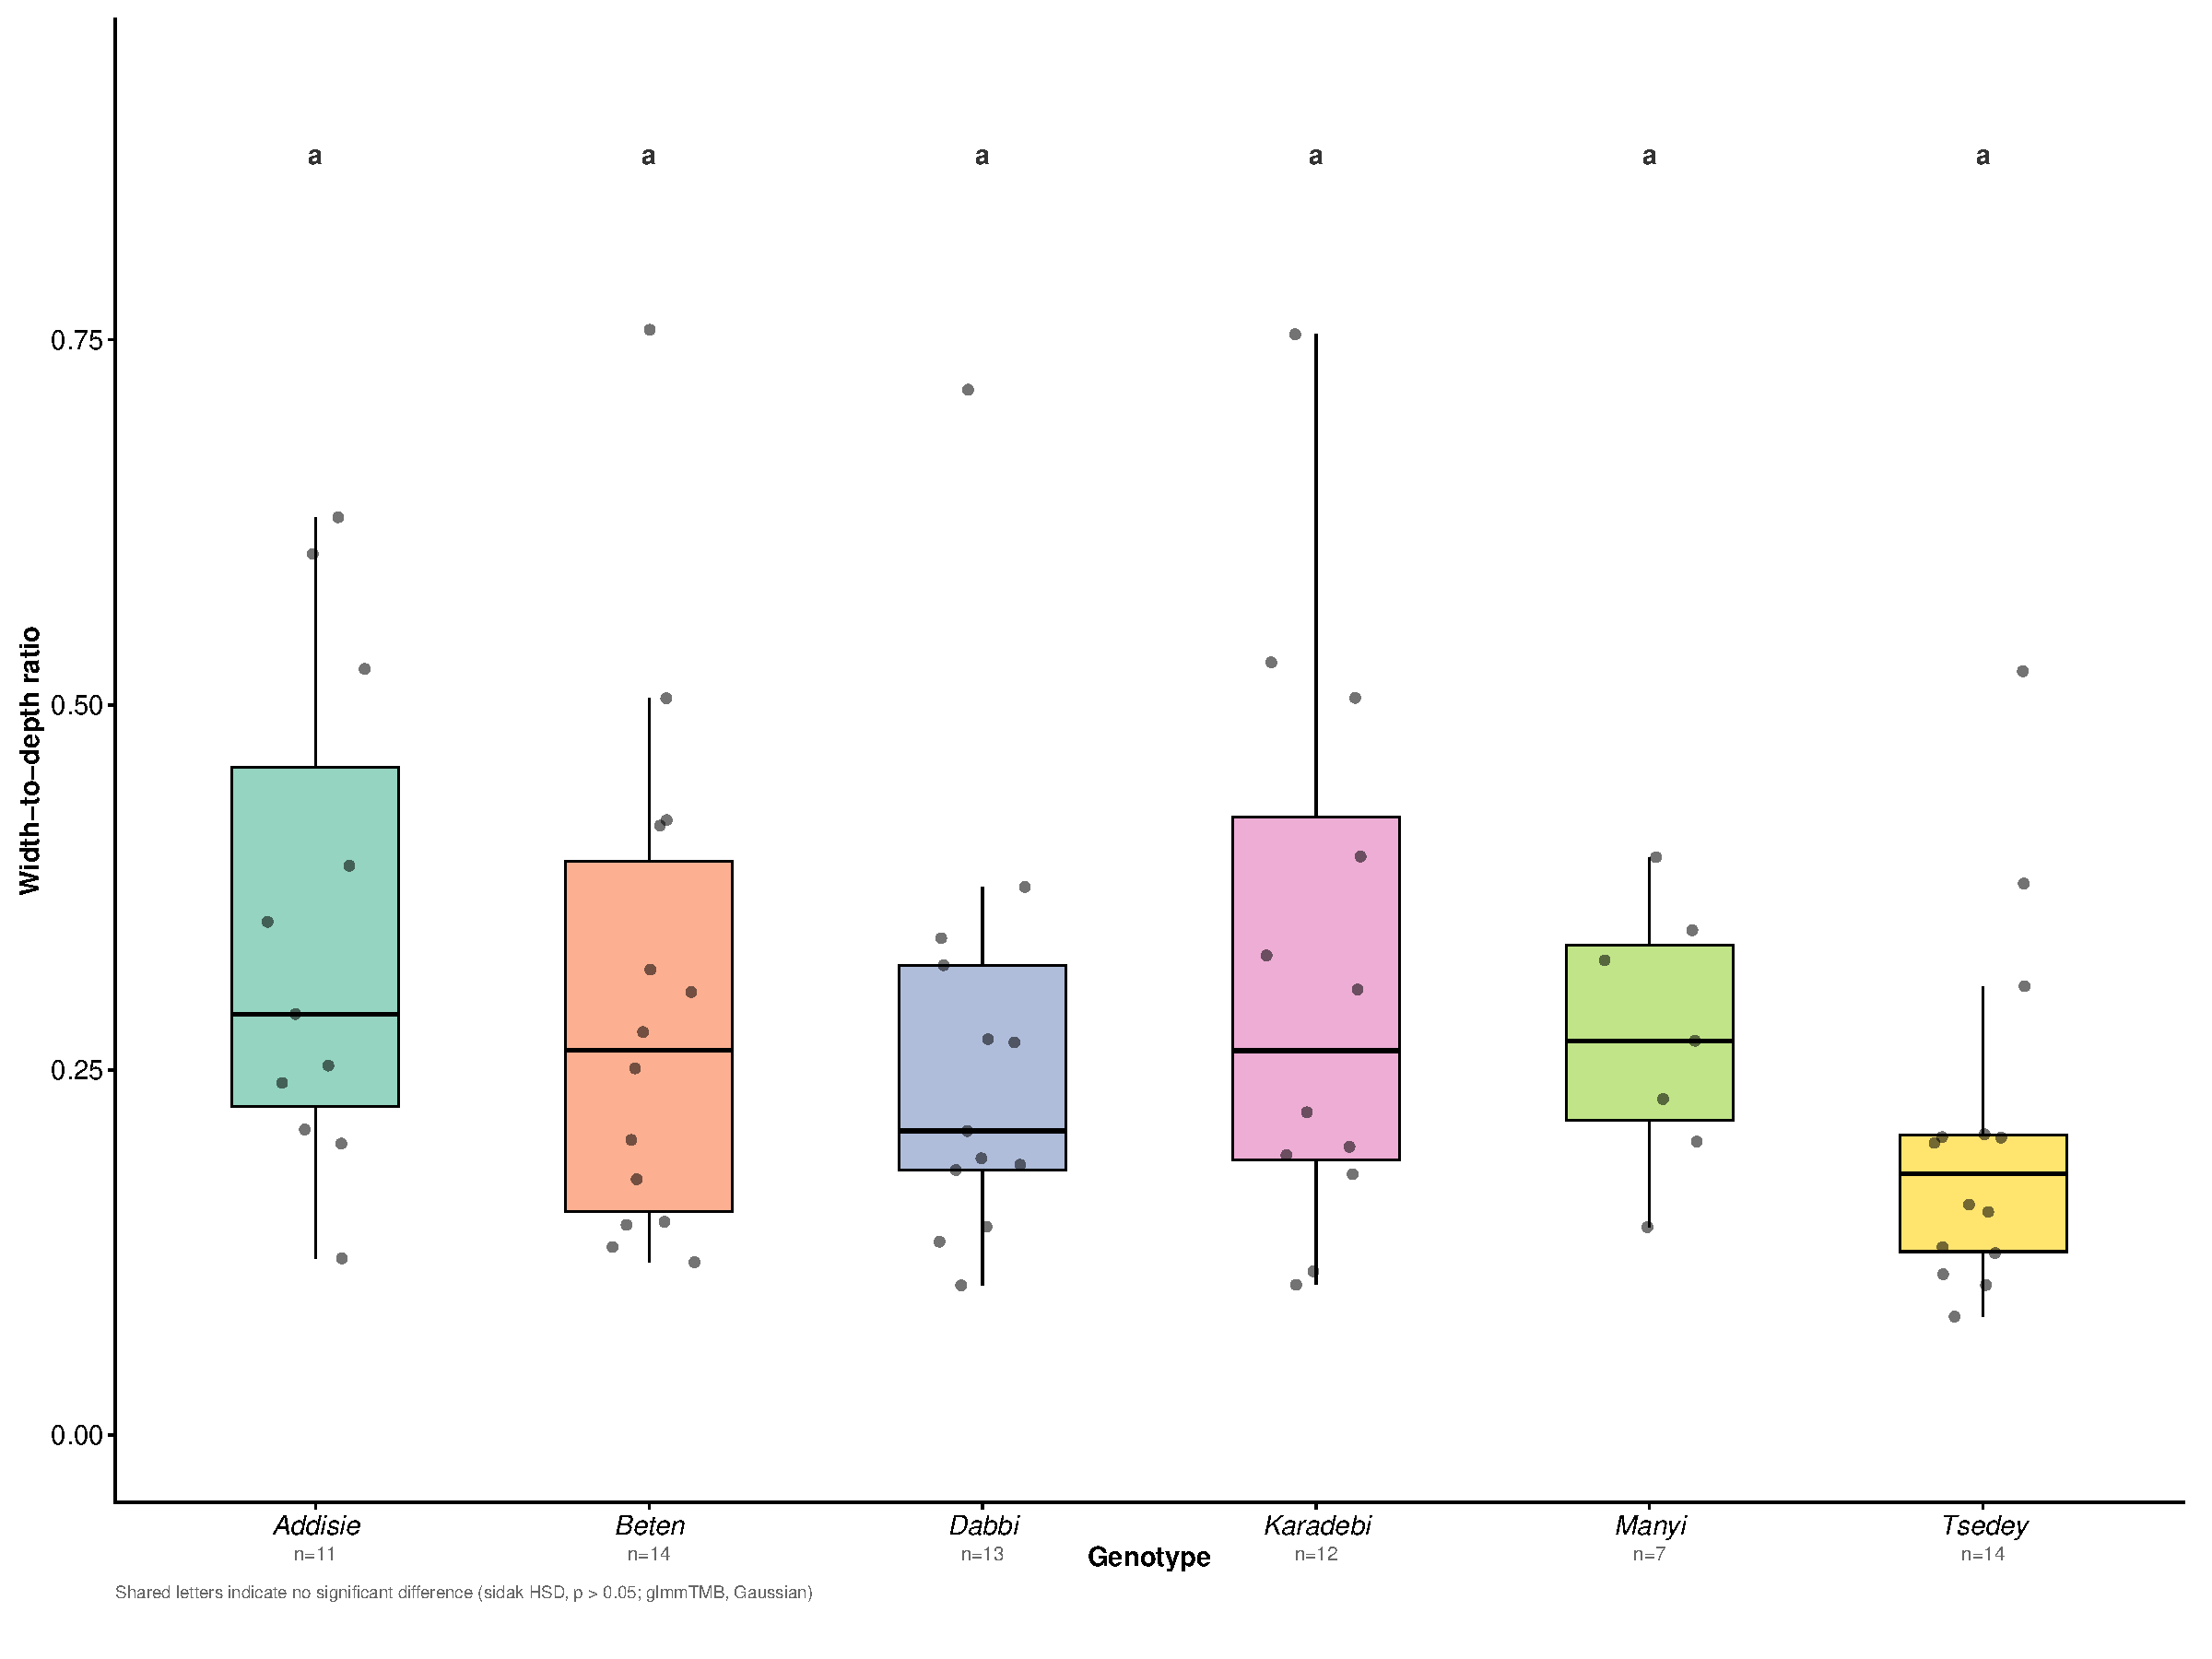
\includegraphics[keepaspectratio]{rsa_day1617_agar_files/figure-pdf/unnamed-chunk-8-10.pdf}}

\begin{Shaded}
\begin{Highlighting}[]
\CommentTok{\# this is the same result as the model with no random effects included so happy to continue with this result.}
\end{Highlighting}
\end{Shaded}

\subsubsection{Steep Angle Frequency}\label{steep-angle-frequency}

\begin{Shaded}
\begin{Highlighting}[]
\CommentTok{\# ============================================================}
\CommentTok{\#  Steep Angle Frequency Analysis}
\CommentTok{\#  Frequency/proportion bounded 0{-}1 — Beta regression}
\CommentTok{\#  Check for exact 0s or 1s before fitting}
\CommentTok{\# ============================================================}

\CommentTok{\# Per{-}genotype Var/Mean — Poisson assumes Var = Mean exactly.}
\CommentTok{\# Ratios \textgreater{}\textgreater{} 1 within genotypes suggest NB is needed.}
\NormalTok{df }\SpecialCharTok{\%\textgreater{}\%}
  \FunctionTok{group\_by}\NormalTok{(Genotype) }\SpecialCharTok{\%\textgreater{}\%}
  \FunctionTok{summarise}\NormalTok{(}\AttributeTok{Mean     =} \FunctionTok{round}\NormalTok{(}\FunctionTok{mean}\NormalTok{(Steep.Angle.Frequency), }\DecValTok{2}\NormalTok{),}
            \AttributeTok{Variance =} \FunctionTok{round}\NormalTok{(}\FunctionTok{var}\NormalTok{(Steep.Angle.Frequency),  }\DecValTok{2}\NormalTok{),}
            \AttributeTok{Var\_Mean =} \FunctionTok{round}\NormalTok{(}\FunctionTok{var}\NormalTok{(Steep.Angle.Frequency) }\SpecialCharTok{/}
                               \FunctionTok{mean}\NormalTok{(Steep.Angle.Frequency), }\DecValTok{2}\NormalTok{))}
\end{Highlighting}
\end{Shaded}

\begin{verbatim}
# A tibble: 6 x 4
  Genotype  Mean Variance Var_Mean
  <fct>    <dbl>    <dbl>    <dbl>
1 Addisie   0.73     0.02     0.03
2 Beten     0.78     0.01     0.01
3 Dabbi     0.76     0.01     0.02
4 Karadebi  0.76     0.02     0.03
5 Manyi     0.75     0        0   
6 Tsedey    0.88     0.01     0.01
\end{verbatim}

\begin{Shaded}
\begin{Highlighting}[]
\CommentTok{\# ── 1. Inspect distribution ───────────────────────────────────}
\FunctionTok{summary}\NormalTok{(df}\SpecialCharTok{$}\NormalTok{Steep.Angle.Frequency)}
\end{Highlighting}
\end{Shaded}

\begin{verbatim}
   Min. 1st Qu.  Median    Mean 3rd Qu.    Max. 
 0.4804  0.7123  0.7931  0.7811  0.8784  0.9709 
\end{verbatim}

\begin{Shaded}
\begin{Highlighting}[]
\FunctionTok{hist}\NormalTok{(df}\SpecialCharTok{$}\NormalTok{Steep.Angle.Frequency, }\AttributeTok{breaks =} \DecValTok{15}\NormalTok{, }\AttributeTok{main =} \StringTok{"Steep Angle Frequency distribution"}\NormalTok{)}
\end{Highlighting}
\end{Shaded}

\pandocbounded{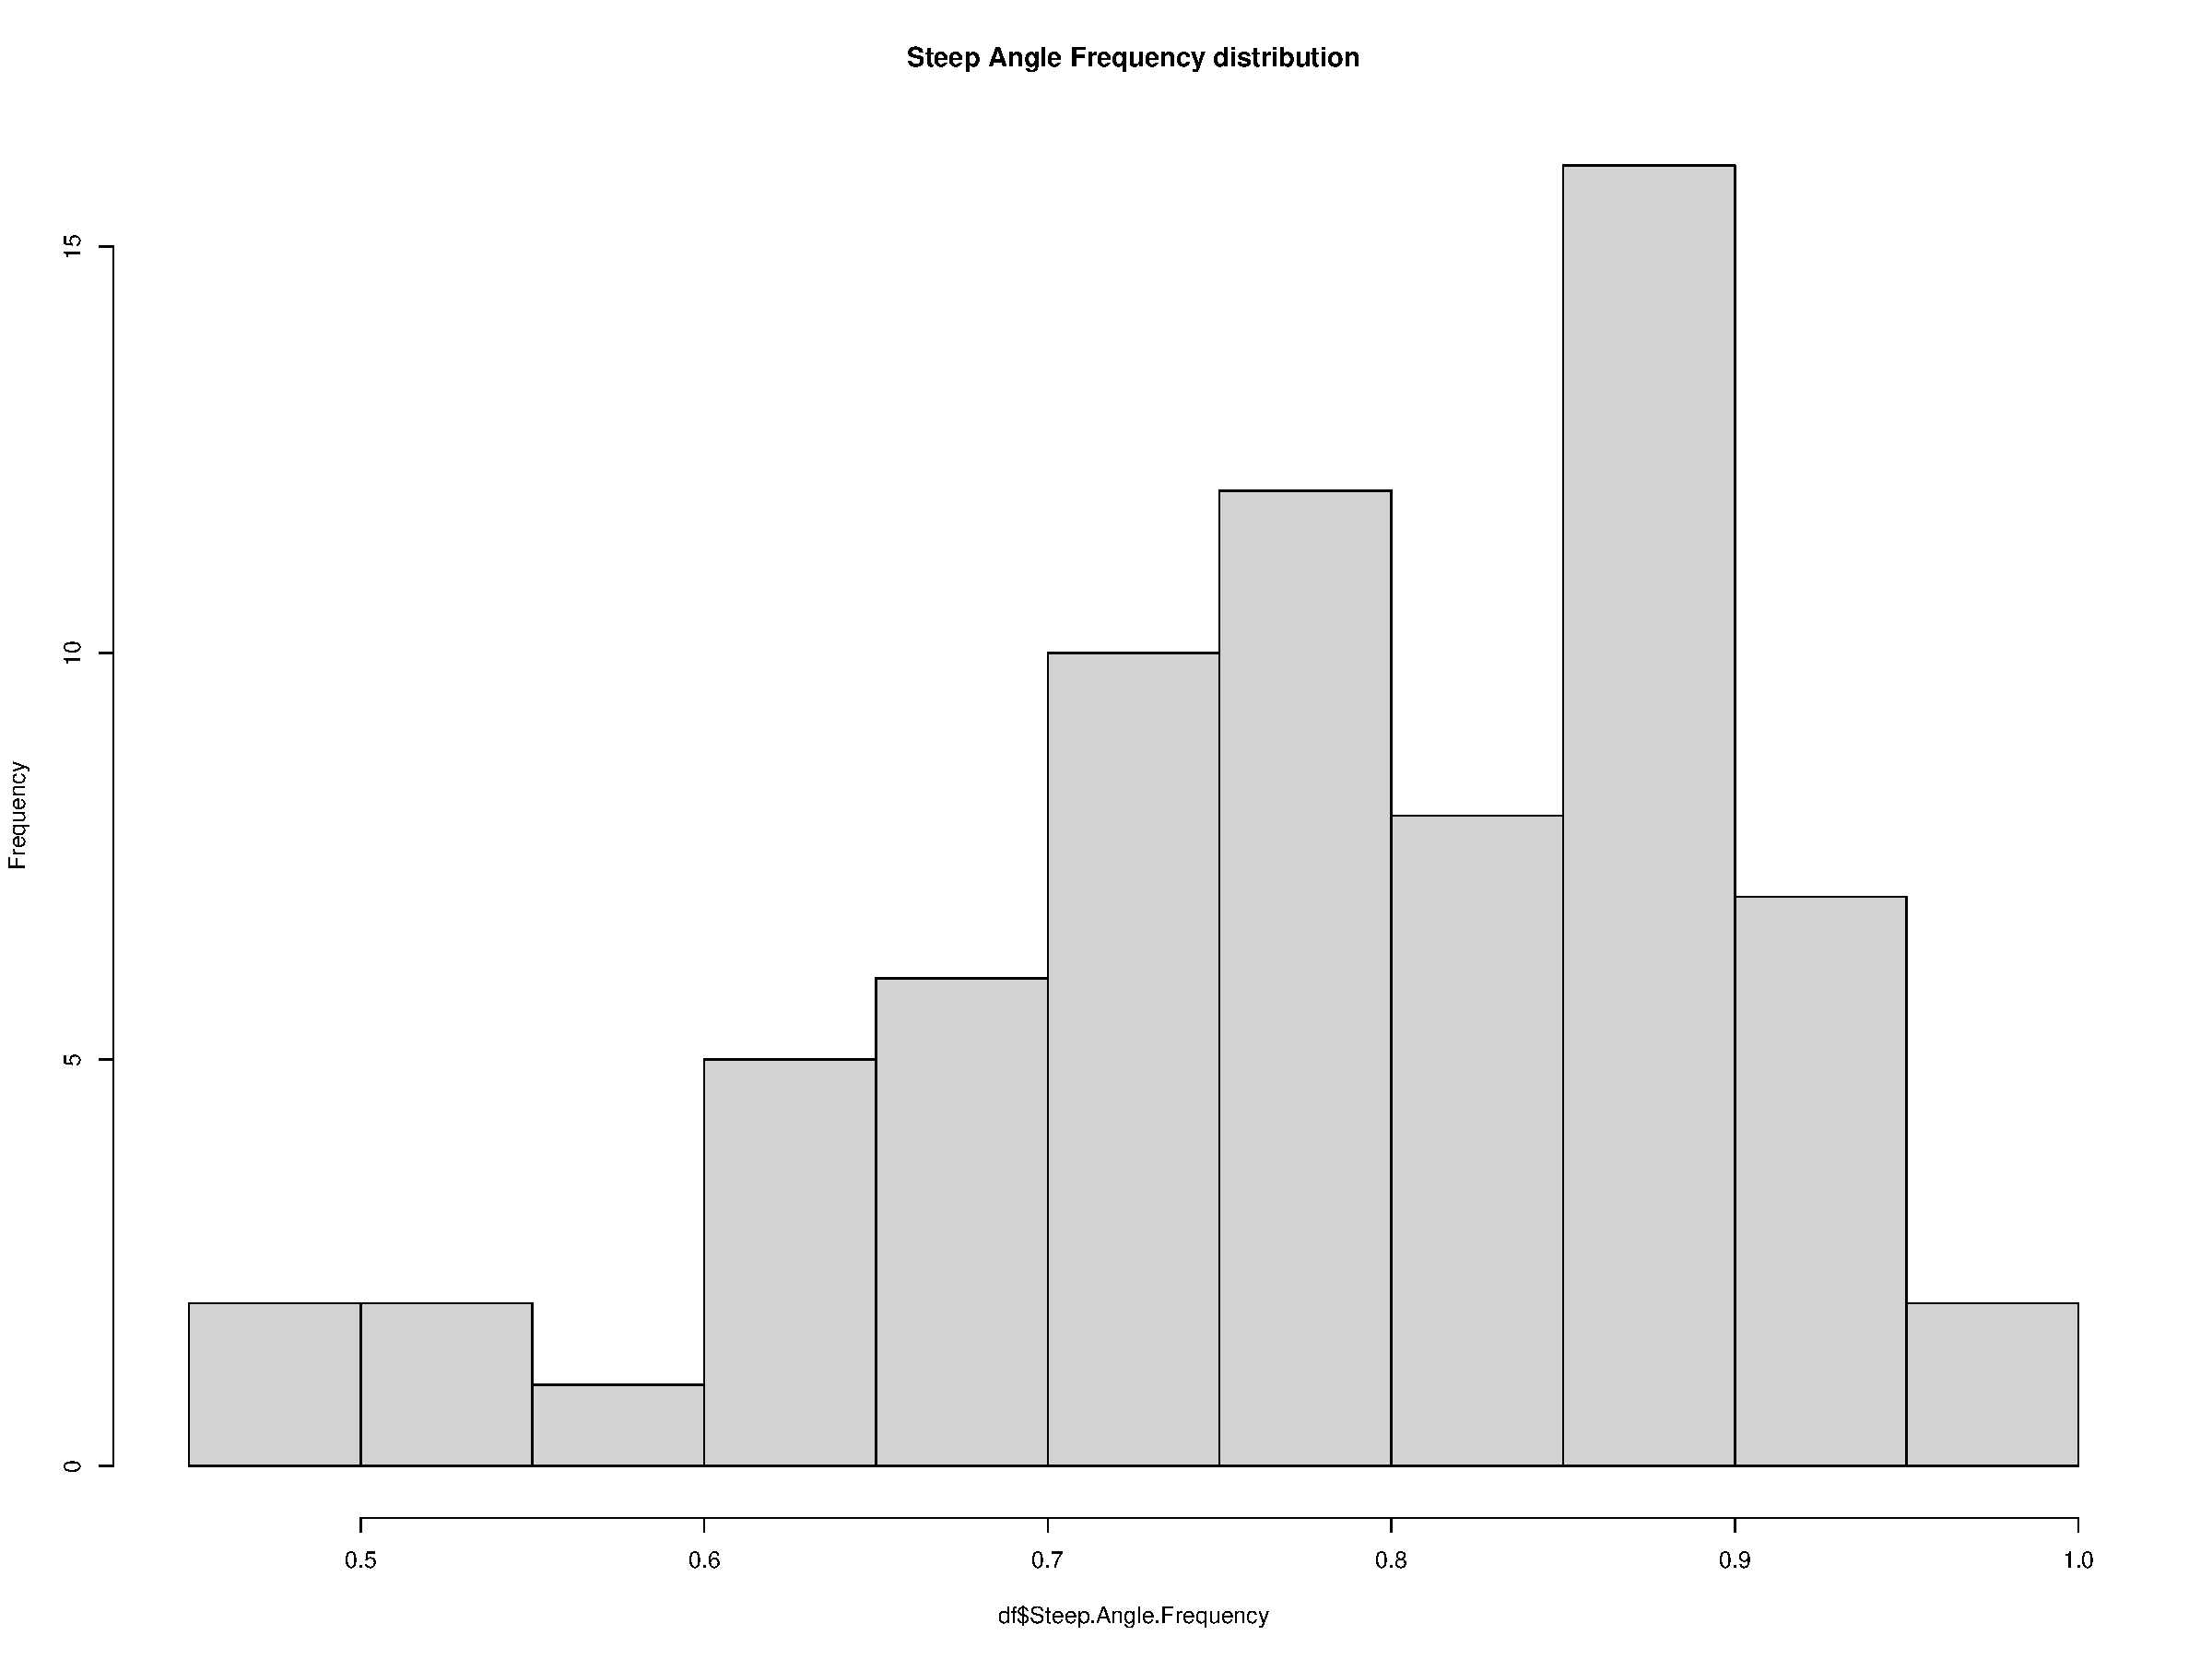
\includegraphics[keepaspectratio]{rsa_day1617_agar_files/figure-pdf/unnamed-chunk-9-1.pdf}}

\begin{Shaded}
\begin{Highlighting}[]
\CommentTok{\# Check for exact 0s or 1s — Beta cannot handle boundary values}
\FunctionTok{sum}\NormalTok{(df}\SpecialCharTok{$}\NormalTok{Steep.Angle.Frequency }\SpecialCharTok{==} \DecValTok{0}\NormalTok{)}
\end{Highlighting}
\end{Shaded}

\begin{verbatim}
[1] 0
\end{verbatim}

\begin{Shaded}
\begin{Highlighting}[]
\FunctionTok{sum}\NormalTok{(df}\SpecialCharTok{$}\NormalTok{Steep.Angle.Frequency }\SpecialCharTok{==} \DecValTok{1}\NormalTok{)}
\end{Highlighting}
\end{Shaded}

\begin{verbatim}
[1] 0
\end{verbatim}

\begin{Shaded}
\begin{Highlighting}[]
\CommentTok{\# If any exist, apply small boundary correction:}
\CommentTok{\# df$Steep.Angle.Frequency \textless{}{-} (df$Steep.Angle.Frequency * (nrow(df) {-} 1) + 0.5) / nrow(df)}


\CommentTok{\# ── 2. Fit full nested model ──────────────────────────────────}
\NormalTok{steep\_full }\OtherTok{\textless{}{-}} \FunctionTok{glmmTMB}\NormalTok{(}
\NormalTok{  Steep.Angle.Frequency }\SpecialCharTok{\textasciitilde{}}\NormalTok{ Genotype }\SpecialCharTok{+}\NormalTok{ (}\DecValTok{1} \SpecialCharTok{|}\NormalTok{ Batch}\SpecialCharTok{/}\NormalTok{Plate}\SpecialCharTok{/}\NormalTok{Seed),}
  \AttributeTok{data =}\NormalTok{ df, }\AttributeTok{family =} \FunctionTok{beta\_family}\NormalTok{()}
\NormalTok{)}

\FunctionTok{VarCorr}\NormalTok{(steep\_full)}
\end{Highlighting}
\end{Shaded}

\begin{verbatim}

Conditional model:
 Groups           Name        Std.Dev.  
 Seed:Plate:Batch (Intercept) 5.5609e-05
 Plate:Batch      (Intercept) 1.8745e-01
 Batch            (Intercept) 1.9521e-07
\end{verbatim}

\begin{Shaded}
\begin{Highlighting}[]
\FunctionTok{check\_singularity}\NormalTok{(steep\_full)}
\end{Highlighting}
\end{Shaded}

\begin{verbatim}
[1] TRUE
\end{verbatim}

\begin{Shaded}
\begin{Highlighting}[]
\FunctionTok{summary}\NormalTok{(steep\_full)}
\end{Highlighting}
\end{Shaded}

\begin{verbatim}
 Family: beta  ( logit )
Formula:          Steep.Angle.Frequency ~ Genotype + (1 | Batch/Plate/Seed)
Data: df

      AIC       BIC    logLik -2*log(L)  df.resid 
   -115.8     -93.1      67.9    -135.8        61 

Random effects:

Conditional model:
 Groups           Name        Variance  Std.Dev. 
 Seed:Plate:Batch (Intercept) 3.092e-09 5.561e-05
 Plate:Batch      (Intercept) 3.514e-02 1.874e-01
 Batch            (Intercept) 3.811e-14 1.952e-07
Number of obs: 71, groups:  Seed:Plate:Batch, 38; Plate:Batch, 18; Batch, 4

Dispersion parameter for beta family (): 17.8 

Conditional model:
                  Estimate Std. Error z value Pr(>|z|)    
(Intercept)      1.0101892  0.1705431   5.923 3.15e-09 ***
GenotypeBeten    0.2545476  0.2159140   1.179 0.238426    
GenotypeDabbi    0.1804790  0.2445004   0.738 0.460421    
GenotypeKaradebi 0.1616736  0.2291491   0.706 0.480475    
GenotypeManyi    0.0002391  0.2657766   0.001 0.999282    
GenotypeTsedey   0.9057910  0.2417281   3.747 0.000179 ***
---
Signif. codes:  0 '***' 0.001 '**' 0.01 '*' 0.05 '.' 0.1 ' ' 1
\end{verbatim}

\begin{Shaded}
\begin{Highlighting}[]
\CommentTok{\# assumptions}

\NormalTok{sim\_res }\OtherTok{\textless{}{-}} \FunctionTok{simulateResiduals}\NormalTok{(steep\_full, }\AttributeTok{n =} \DecValTok{1000}\NormalTok{)}
\FunctionTok{plot}\NormalTok{(sim\_res)}
\end{Highlighting}
\end{Shaded}

\pandocbounded{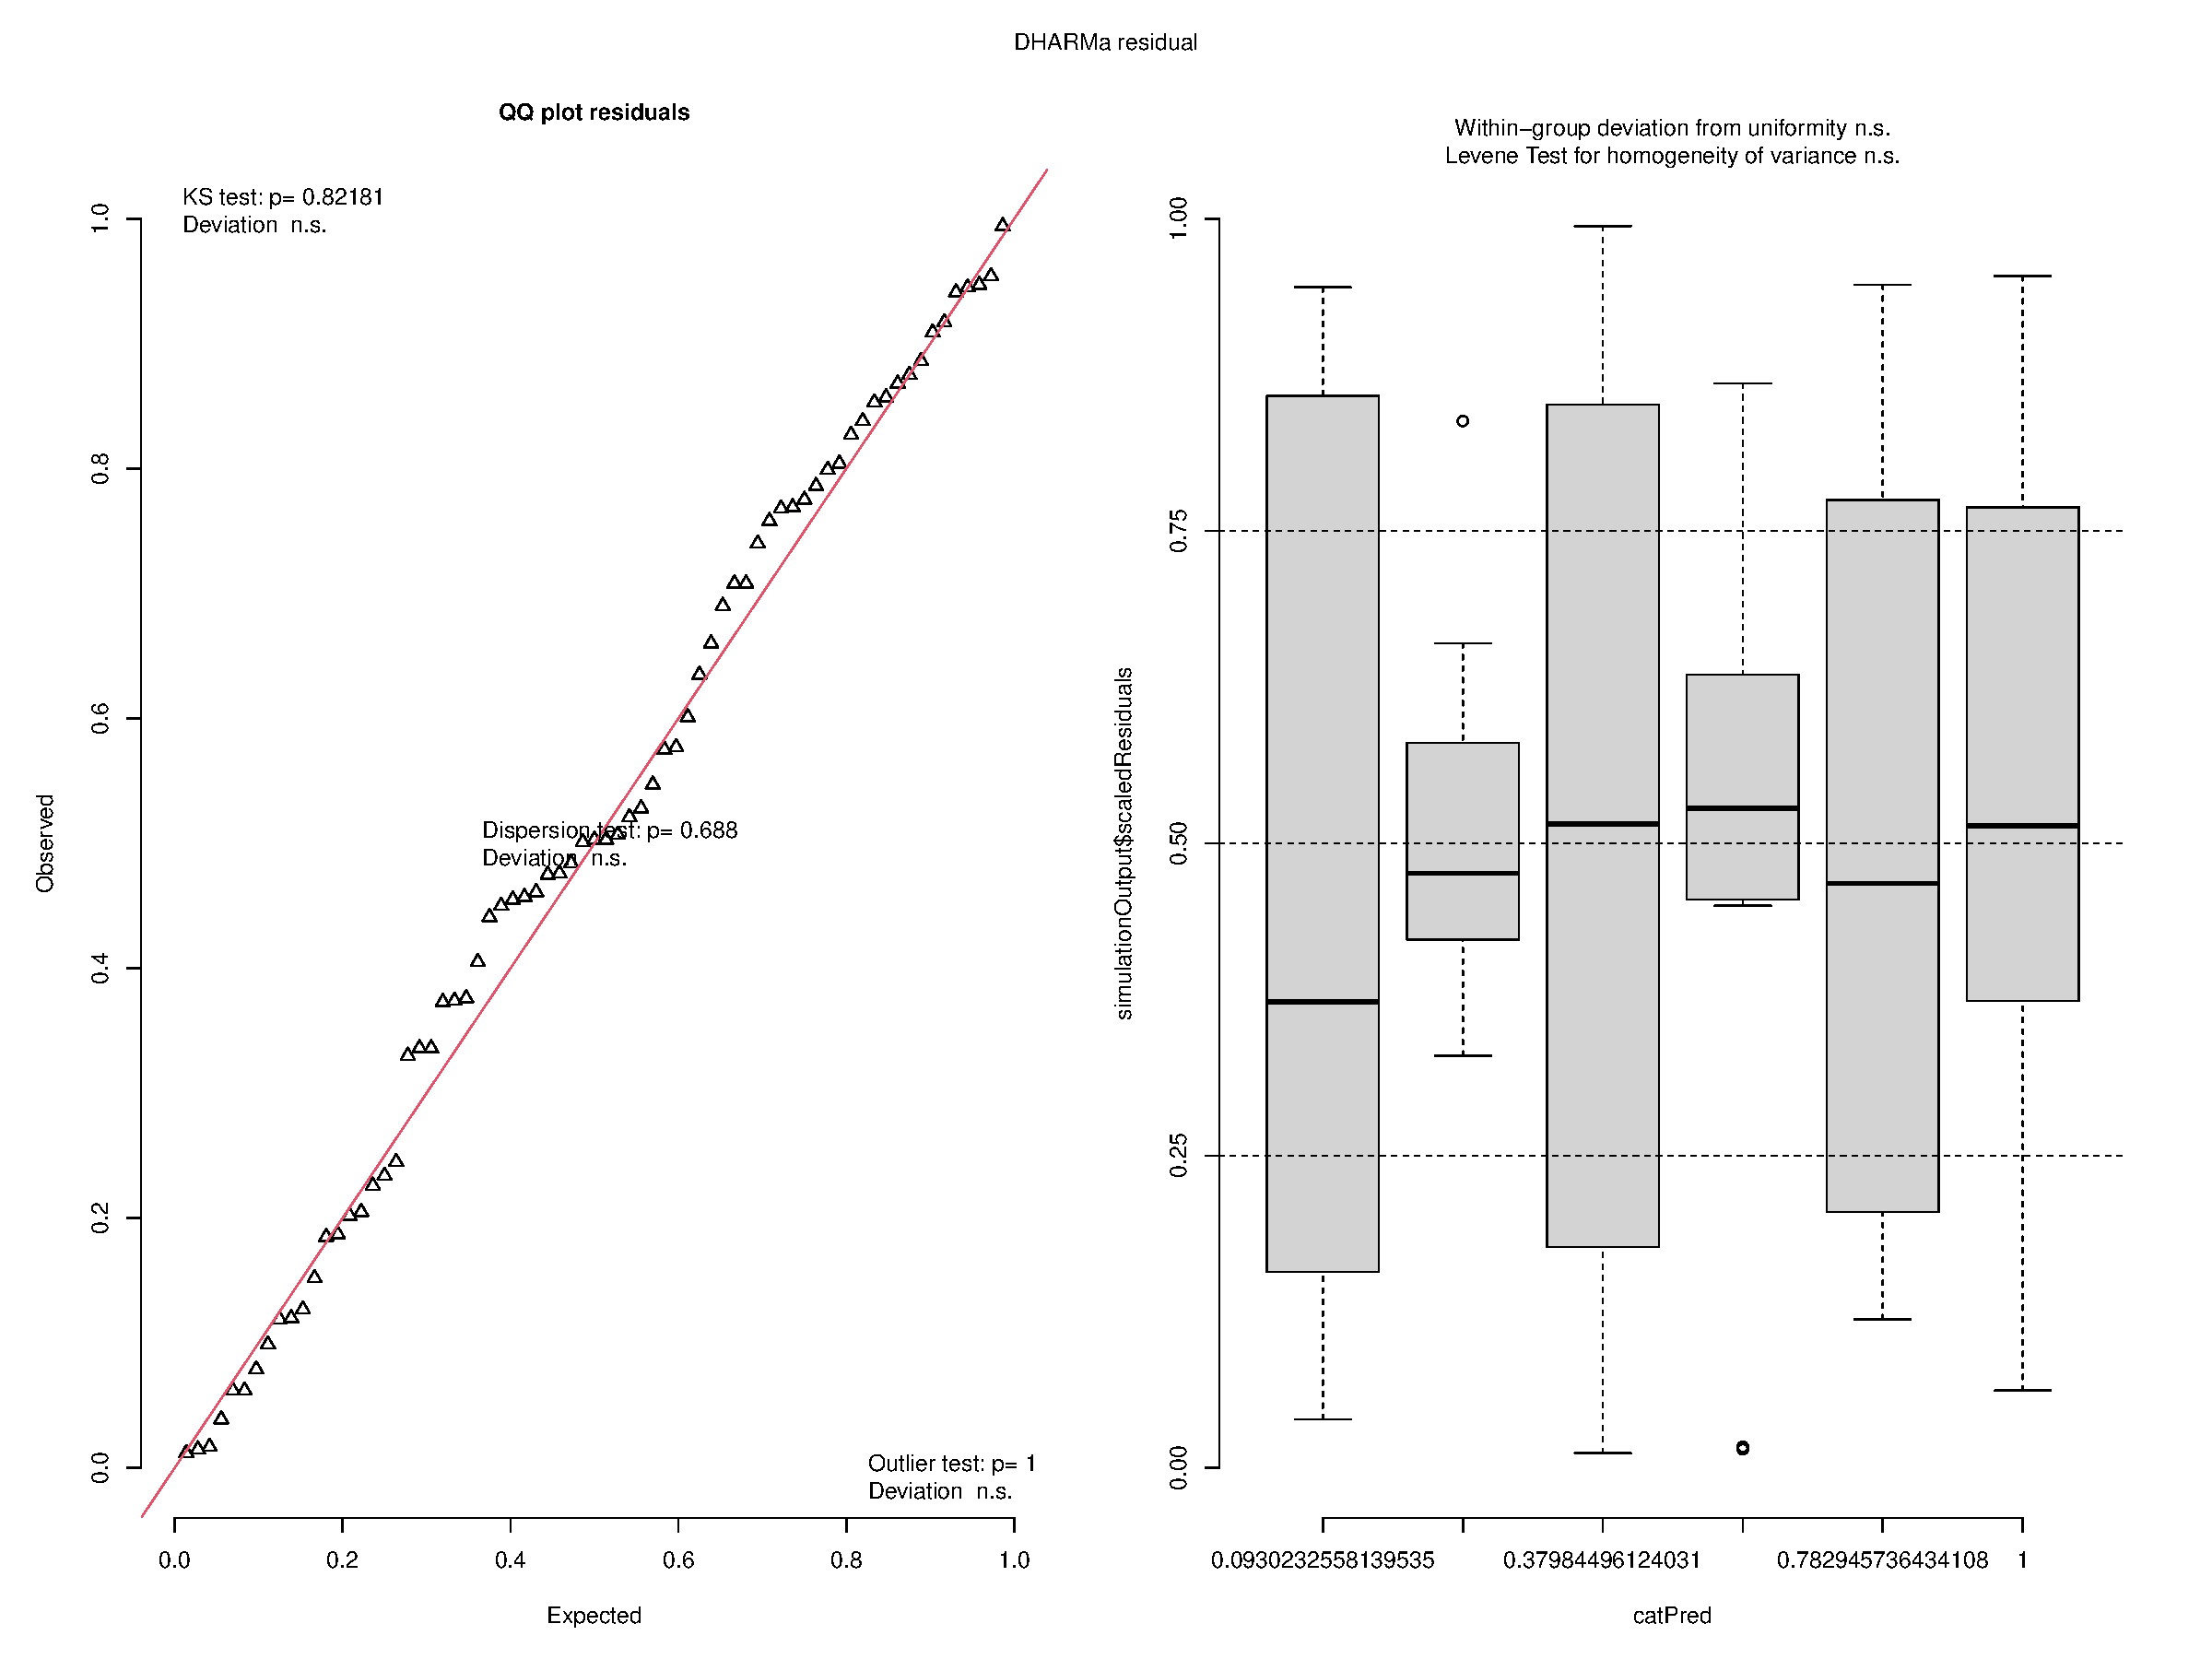
\includegraphics[keepaspectratio]{rsa_day1617_agar_files/figure-pdf/unnamed-chunk-9-2.pdf}}

\begin{Shaded}
\begin{Highlighting}[]
\FunctionTok{testUniformity}\NormalTok{(sim\_res)                     }\CommentTok{\# p \textgreater{} 0.05 = Beta appropriate}
\end{Highlighting}
\end{Shaded}

\pandocbounded{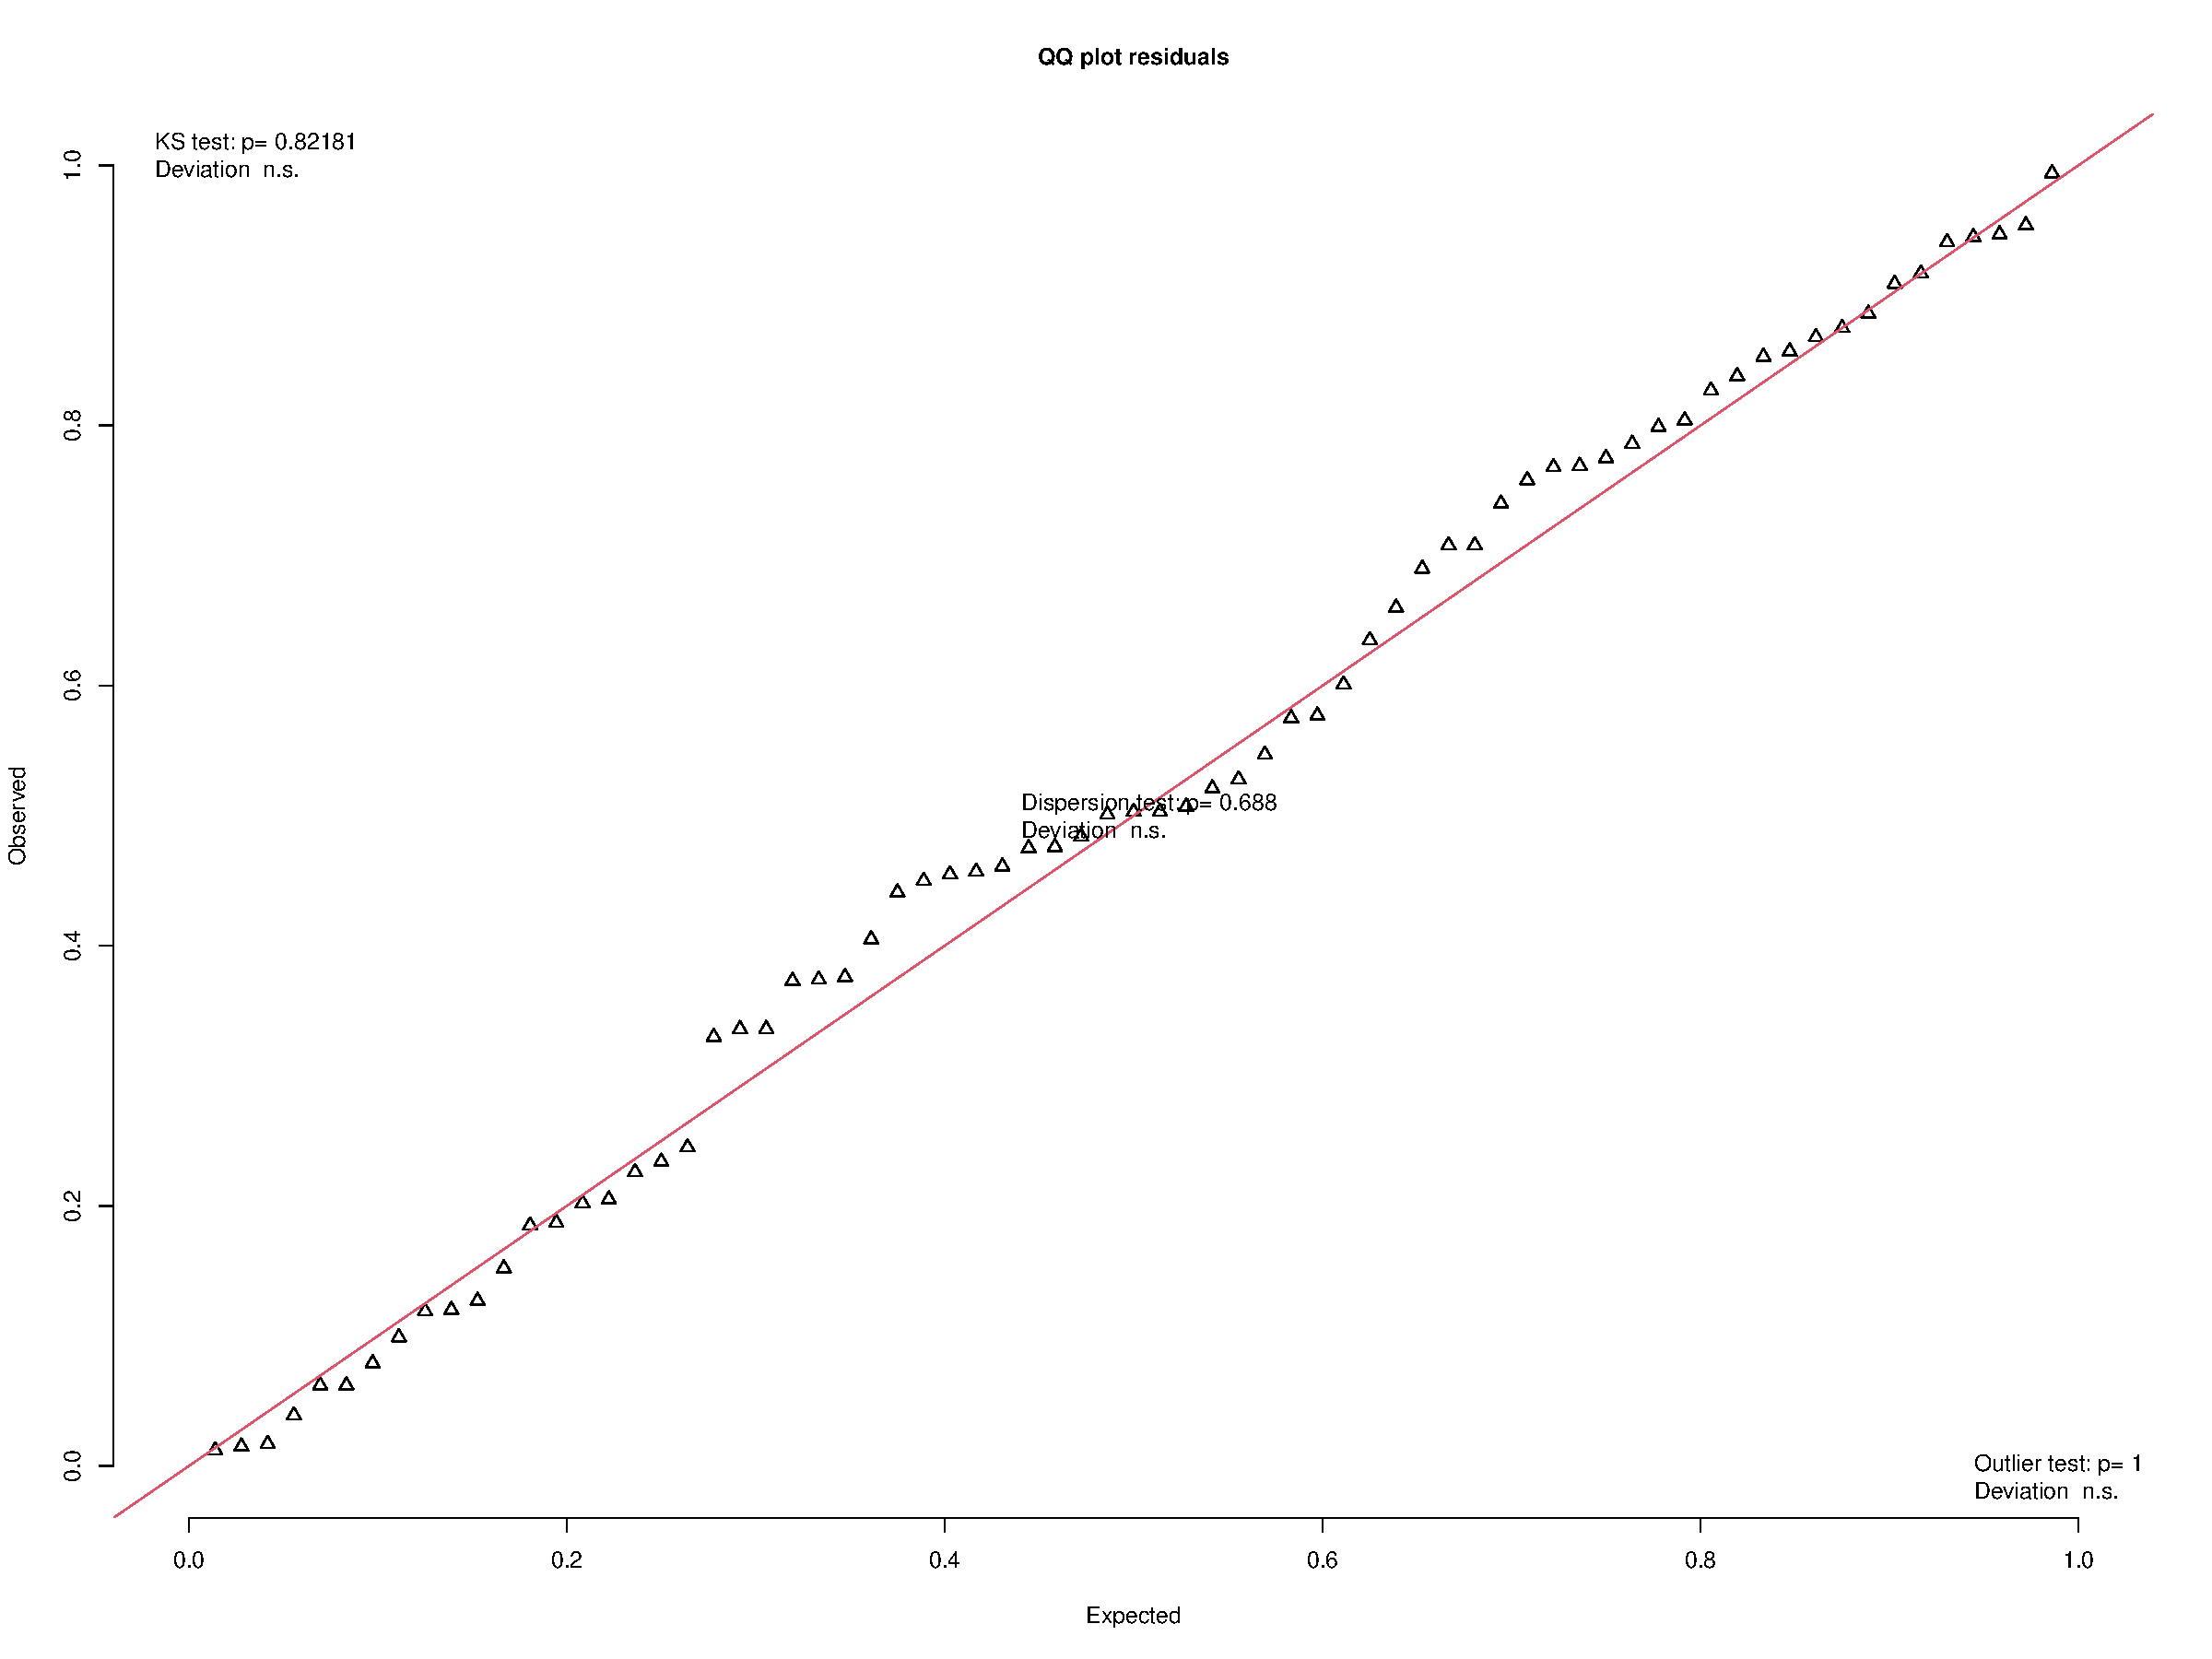
\includegraphics[keepaspectratio]{rsa_day1617_agar_files/figure-pdf/unnamed-chunk-9-3.pdf}}

\begin{verbatim}

    Asymptotic one-sample Kolmogorov-Smirnov test

data:  simulationOutput$scaledResiduals
D = 0.074803, p-value = 0.8218
alternative hypothesis: two-sided
\end{verbatim}

\begin{Shaded}
\begin{Highlighting}[]
\FunctionTok{testDispersion}\NormalTok{(sim\_res)                     }\CommentTok{\# ratio ≈ 1.0}
\end{Highlighting}
\end{Shaded}

\pandocbounded{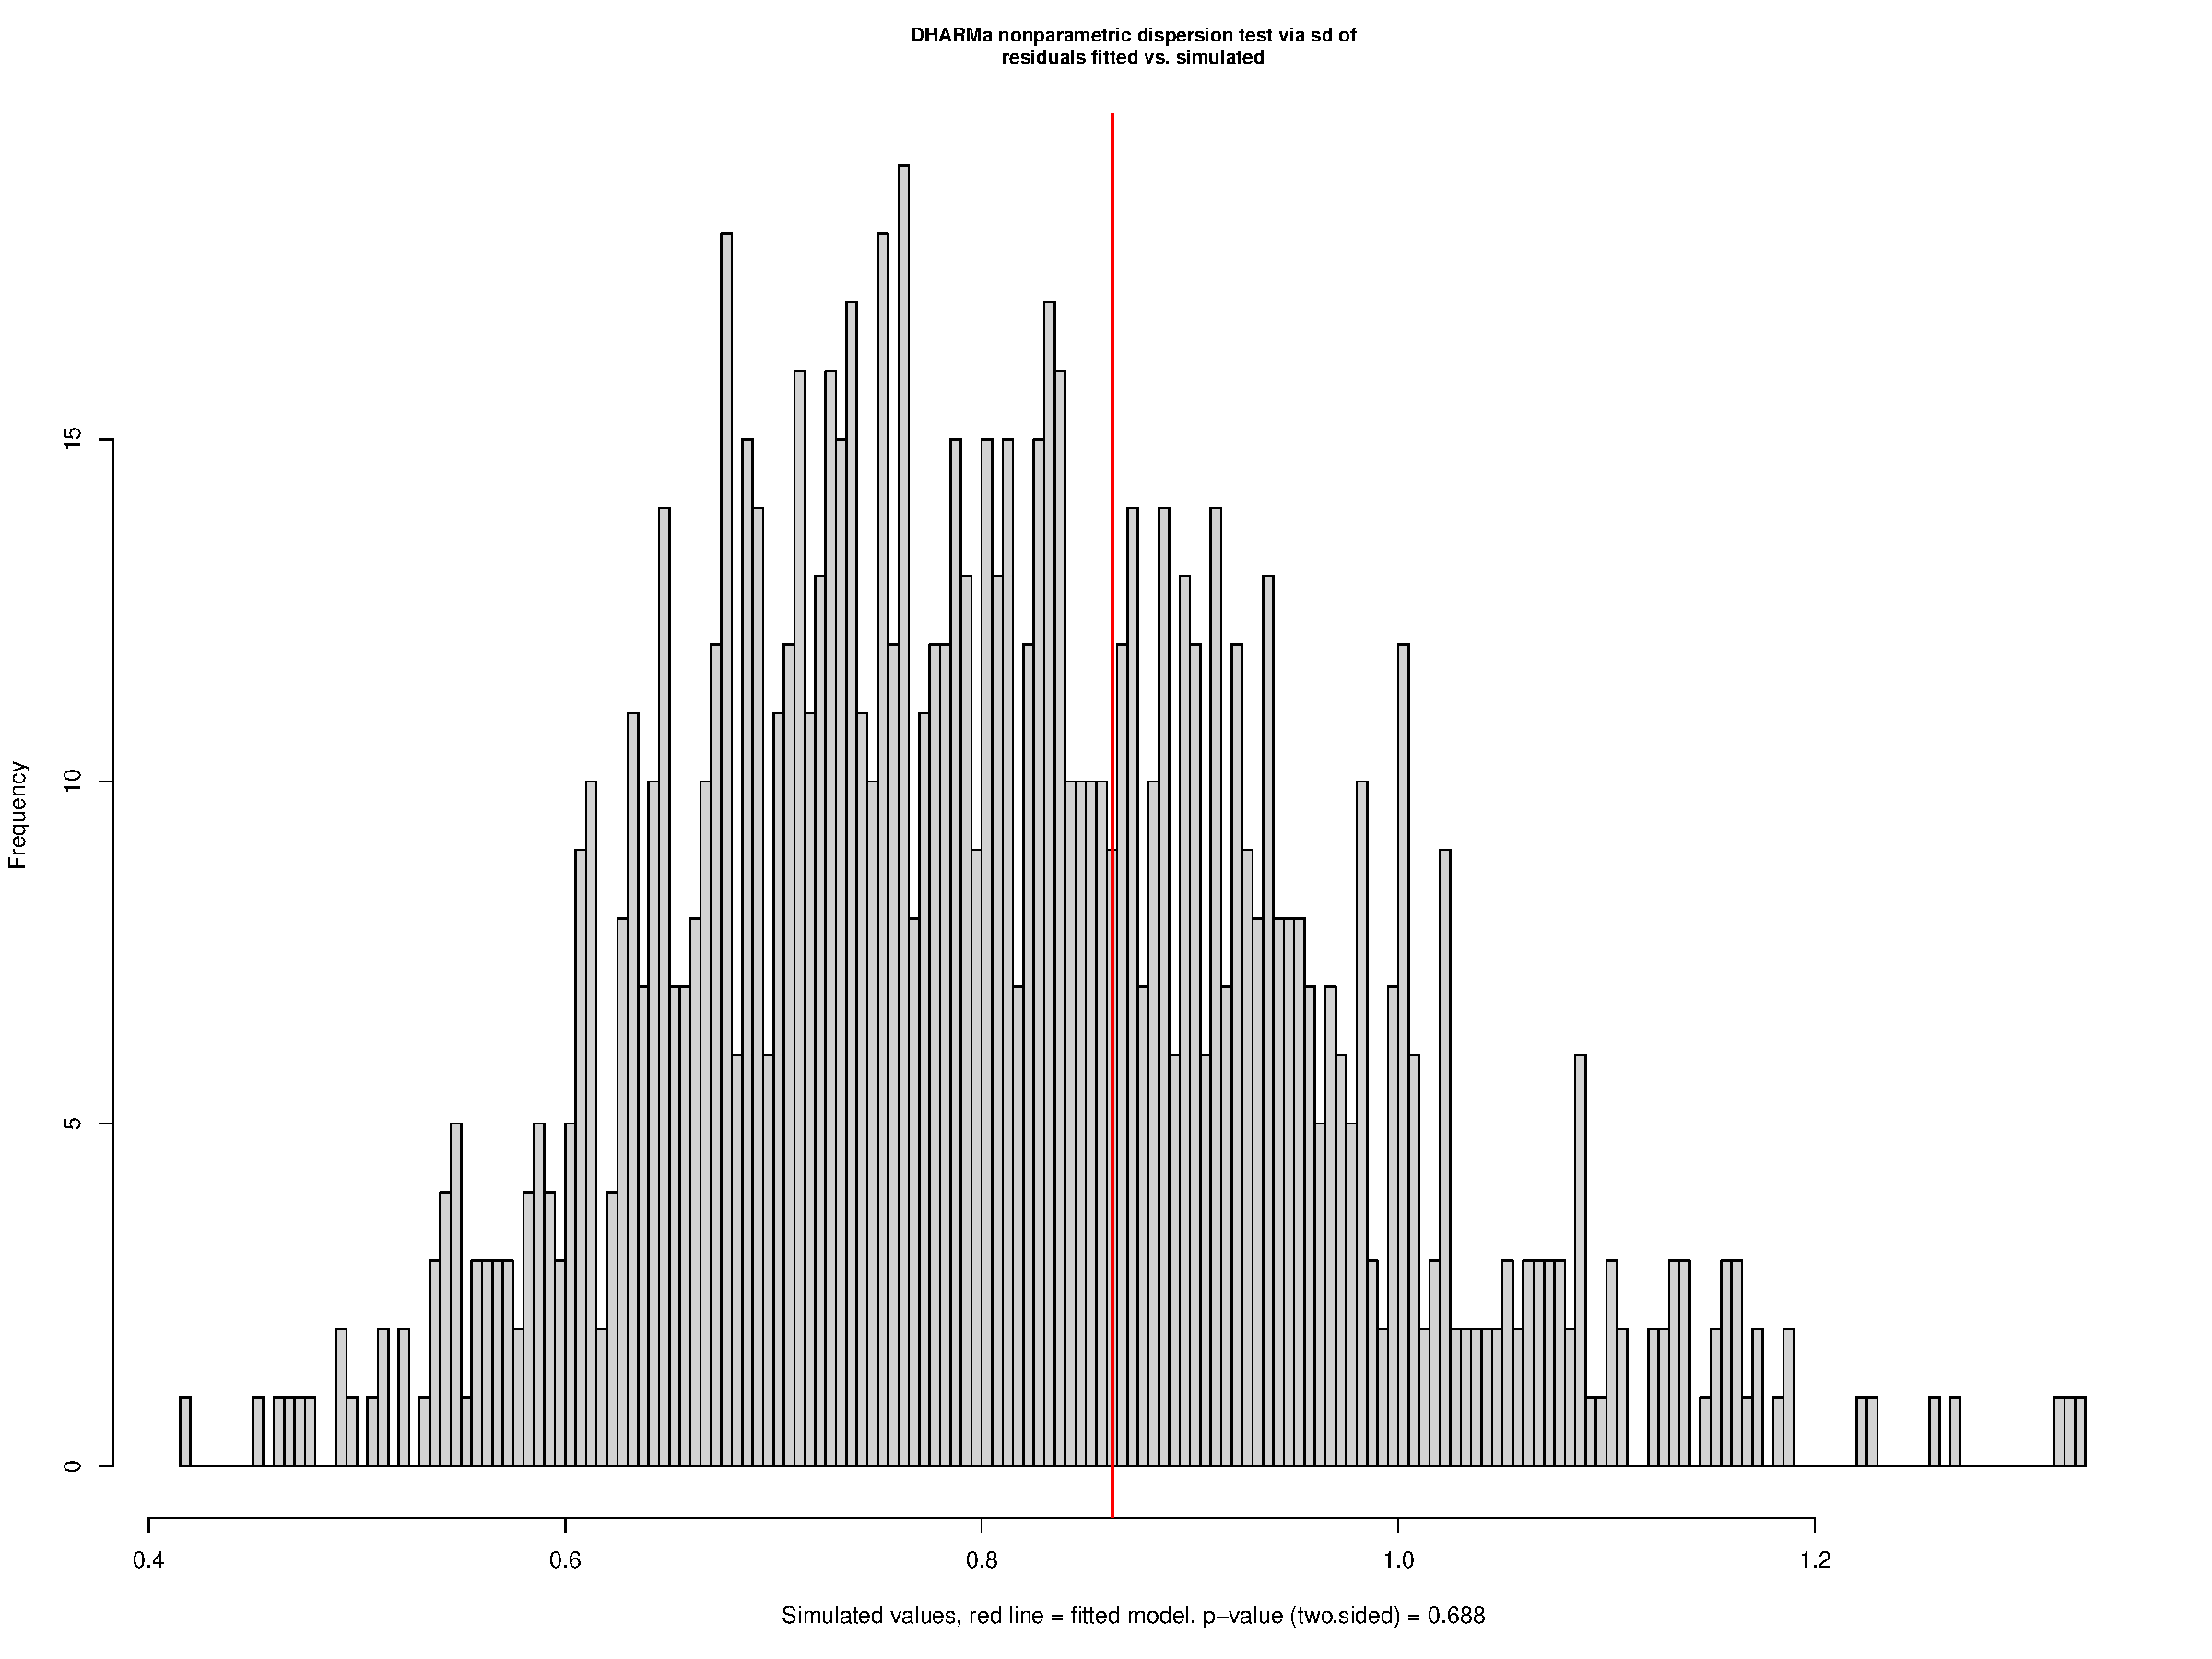
\includegraphics[keepaspectratio]{rsa_day1617_agar_files/figure-pdf/unnamed-chunk-9-4.pdf}}

\begin{verbatim}

    DHARMa nonparametric dispersion test via sd of residuals fitted vs.
    simulated

data:  simulationOutput
dispersion = 1.0658, p-value = 0.688
alternative hypothesis: two.sided
\end{verbatim}

\begin{Shaded}
\begin{Highlighting}[]
\FunctionTok{plotResiduals}\NormalTok{(sim\_res, }\AttributeTok{form =}\NormalTok{ df}\SpecialCharTok{$}\NormalTok{Genotype)  }\CommentTok{\# no patterns per genotype}
\end{Highlighting}
\end{Shaded}

\pandocbounded{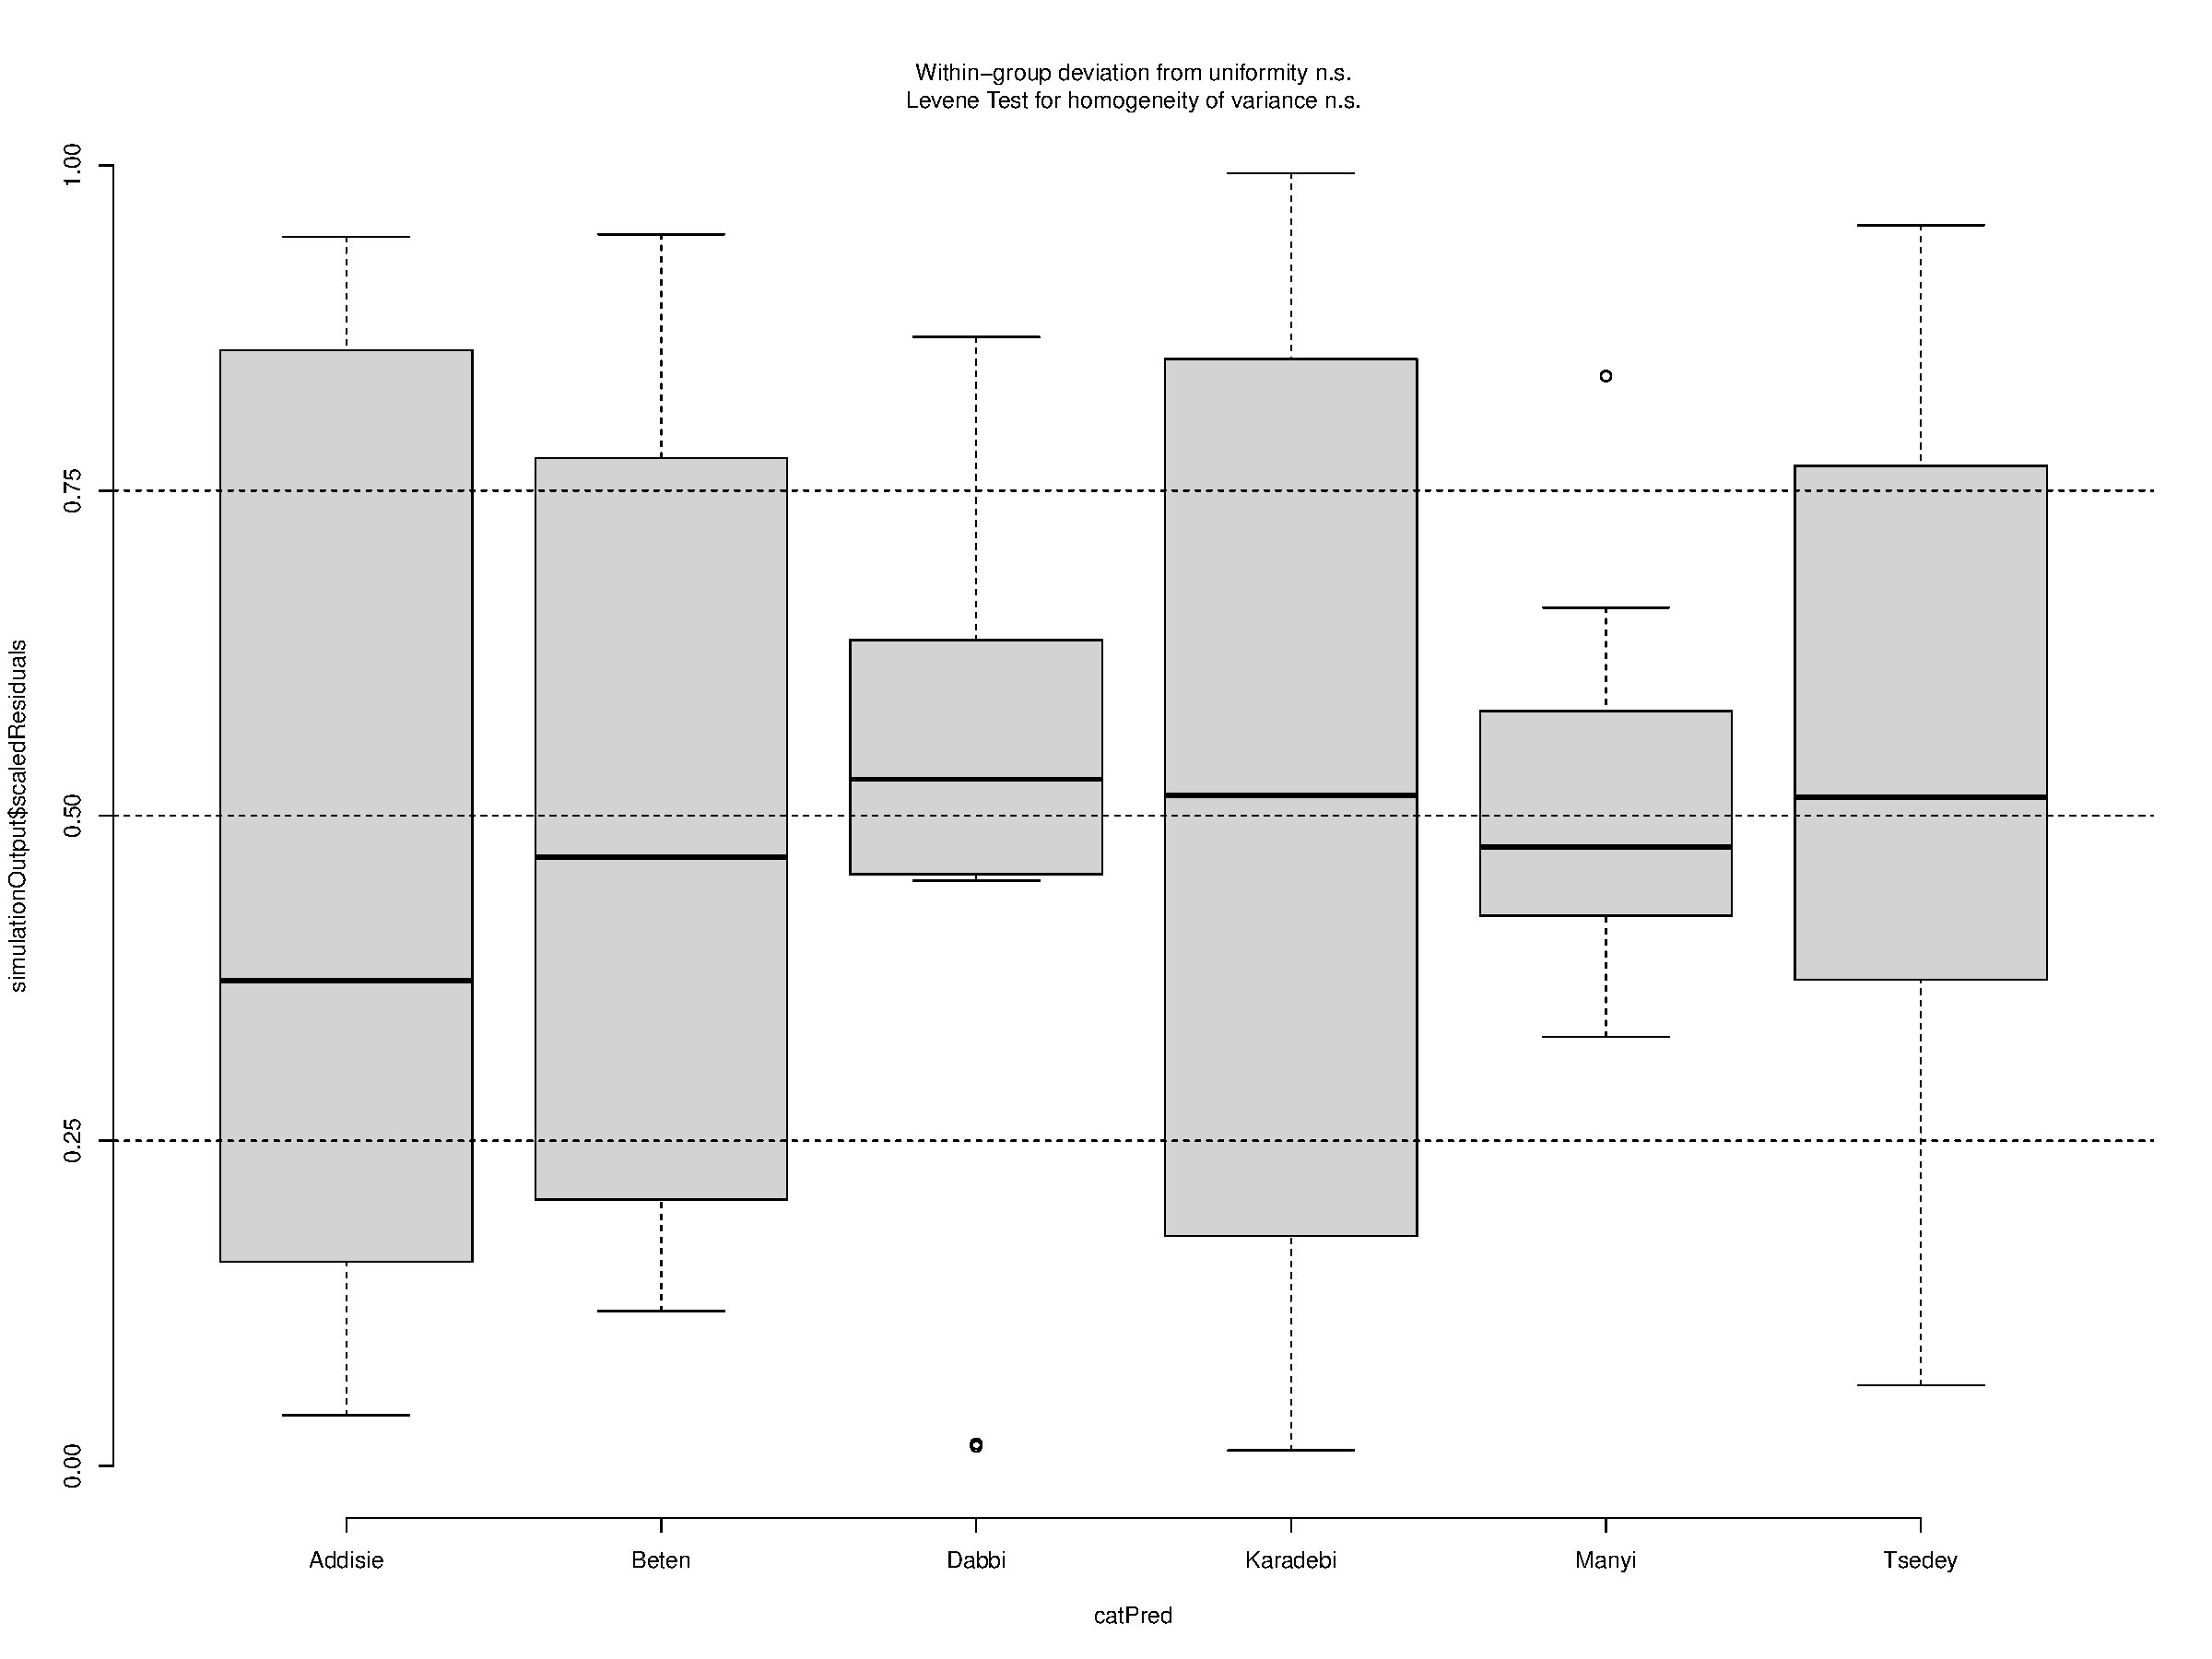
\includegraphics[keepaspectratio]{rsa_day1617_agar_files/figure-pdf/unnamed-chunk-9-5.pdf}}

\begin{Shaded}
\begin{Highlighting}[]
\CommentTok{\# try reducing the model}
\NormalTok{steep\_tmb }\OtherTok{\textless{}{-}} \FunctionTok{glmmTMB}\NormalTok{(}
\NormalTok{  Steep.Angle.Frequency }\SpecialCharTok{\textasciitilde{}}\NormalTok{ Genotype }\SpecialCharTok{+}\NormalTok{ (}\DecValTok{1} \SpecialCharTok{|}\NormalTok{ Batch}\SpecialCharTok{/}\NormalTok{Plate),}
  \AttributeTok{data =}\NormalTok{ df, }\AttributeTok{family =} \FunctionTok{beta\_family}\NormalTok{()}
\NormalTok{)}

\FunctionTok{VarCorr}\NormalTok{(steep\_tmb)}
\end{Highlighting}
\end{Shaded}

\begin{verbatim}

Conditional model:
 Groups      Name        Std.Dev.  
 Plate:Batch (Intercept) 1.8745e-01
 Batch       (Intercept) 2.6408e-05
\end{verbatim}

\begin{Shaded}
\begin{Highlighting}[]
\FunctionTok{check\_singularity}\NormalTok{(steep\_tmb)}
\end{Highlighting}
\end{Shaded}

\begin{verbatim}
[1] TRUE
\end{verbatim}

\begin{Shaded}
\begin{Highlighting}[]
\FunctionTok{summary}\NormalTok{(steep\_tmb)}
\end{Highlighting}
\end{Shaded}

\begin{verbatim}
 Family: beta  ( logit )
Formula:          Steep.Angle.Frequency ~ Genotype + (1 | Batch/Plate)
Data: df

      AIC       BIC    logLik -2*log(L)  df.resid 
   -117.8     -97.4      67.9    -135.8        62 

Random effects:

Conditional model:
 Groups      Name        Variance  Std.Dev. 
 Plate:Batch (Intercept) 3.514e-02 1.874e-01
 Batch       (Intercept) 6.974e-10 2.641e-05
Number of obs: 71, groups:  Plate:Batch, 18; Batch, 4

Dispersion parameter for beta family (): 17.8 

Conditional model:
                  Estimate Std. Error z value Pr(>|z|)    
(Intercept)      1.0101892  0.1705431   5.923 3.15e-09 ***
GenotypeBeten    0.2545476  0.2159140   1.179 0.238426    
GenotypeDabbi    0.1804789  0.2445004   0.738 0.460421    
GenotypeKaradebi 0.1616736  0.2291491   0.706 0.480475    
GenotypeManyi    0.0002391  0.2657766   0.001 0.999282    
GenotypeTsedey   0.9057910  0.2417281   3.747 0.000179 ***
---
Signif. codes:  0 '***' 0.001 '**' 0.01 '*' 0.05 '.' 0.1 ' ' 1
\end{verbatim}

\begin{Shaded}
\begin{Highlighting}[]
\NormalTok{steep\_tmb }\OtherTok{\textless{}{-}} \FunctionTok{glmmTMB}\NormalTok{(}
\NormalTok{  Steep.Angle.Frequency }\SpecialCharTok{\textasciitilde{}}\NormalTok{ Genotype }\SpecialCharTok{+}\NormalTok{ (}\DecValTok{1} \SpecialCharTok{|}\NormalTok{ Batch),}
  \AttributeTok{data =}\NormalTok{ df, }\AttributeTok{family =} \FunctionTok{beta\_family}\NormalTok{()}
\NormalTok{)}

\FunctionTok{VarCorr}\NormalTok{(steep\_tmb)}
\end{Highlighting}
\end{Shaded}

\begin{verbatim}

Conditional model:
 Groups Name        Std.Dev.  
 Batch  (Intercept) 2.2824e-05
\end{verbatim}

\begin{Shaded}
\begin{Highlighting}[]
\FunctionTok{check\_singularity}\NormalTok{(steep\_tmb)}
\end{Highlighting}
\end{Shaded}

\begin{verbatim}
[1] TRUE
\end{verbatim}

\begin{Shaded}
\begin{Highlighting}[]
\FunctionTok{summary}\NormalTok{(steep\_tmb)}
\end{Highlighting}
\end{Shaded}

\begin{verbatim}
 Family: beta  ( logit )
Formula:          Steep.Angle.Frequency ~ Genotype + (1 | Batch)
Data: df

      AIC       BIC    logLik -2*log(L)  df.resid 
   -119.1    -101.0      67.6    -135.1        63 

Random effects:

Conditional model:
 Groups Name        Variance  Std.Dev. 
 Batch  (Intercept) 5.209e-10 2.282e-05
Number of obs: 71, groups:  Batch, 4

Dispersion parameter for beta family (): 16.1 

Conditional model:
                 Estimate Std. Error z value Pr(>|z|)    
(Intercept)      1.019425   0.162585   6.270 3.61e-10 ***
GenotypeBeten    0.250578   0.221964   1.129  0.25893    
GenotypeDabbi    0.113840   0.222658   0.511  0.60916    
GenotypeKaradebi 0.173822   0.228435   0.761  0.44670    
GenotypeManyi    0.006296   0.260153   0.024  0.98069    
GenotypeTsedey   0.893150   0.241712   3.695  0.00022 ***
---
Signif. codes:  0 '***' 0.001 '**' 0.01 '*' 0.05 '.' 0.1 ' ' 1
\end{verbatim}

\begin{Shaded}
\begin{Highlighting}[]
\NormalTok{steep\_tmb }\OtherTok{\textless{}{-}} \FunctionTok{glmmTMB}\NormalTok{(}
\NormalTok{  Steep.Angle.Frequency }\SpecialCharTok{\textasciitilde{}}\NormalTok{ Genotype,}
  \AttributeTok{data =}\NormalTok{ df, }\AttributeTok{family =} \FunctionTok{beta\_family}\NormalTok{()}
\NormalTok{)}

\FunctionTok{summary}\NormalTok{(steep\_tmb)}
\end{Highlighting}
\end{Shaded}

\begin{verbatim}
 Family: beta  ( logit )
Formula:          Steep.Angle.Frequency ~ Genotype
Data: df

      AIC       BIC    logLik -2*log(L)  df.resid 
   -121.1    -105.3      67.6    -135.1        64 


Dispersion parameter for beta family (): 16.1 

Conditional model:
                 Estimate Std. Error z value Pr(>|z|)    
(Intercept)      1.019425   0.162585   6.270 3.61e-10 ***
GenotypeBeten    0.250578   0.221964   1.129  0.25893    
GenotypeDabbi    0.113840   0.222658   0.511  0.60916    
GenotypeKaradebi 0.173822   0.228435   0.761  0.44670    
GenotypeManyi    0.006296   0.260153   0.024  0.98069    
GenotypeTsedey   0.893150   0.241712   3.695  0.00022 ***
---
Signif. codes:  0 '***' 0.001 '**' 0.01 '*' 0.05 '.' 0.1 ' ' 1
\end{verbatim}

\begin{Shaded}
\begin{Highlighting}[]
\CommentTok{\# reduced model does not have homogeneity of variance so full model is probably better. I will try both reduced and full model to see if same result is drawn.}


\CommentTok{\# Assumption checks}

\NormalTok{sim\_res }\OtherTok{\textless{}{-}} \FunctionTok{simulateResiduals}\NormalTok{(steep\_tmb, }\AttributeTok{n =} \DecValTok{1000}\NormalTok{)}
\FunctionTok{plot}\NormalTok{(sim\_res)}
\end{Highlighting}
\end{Shaded}

\pandocbounded{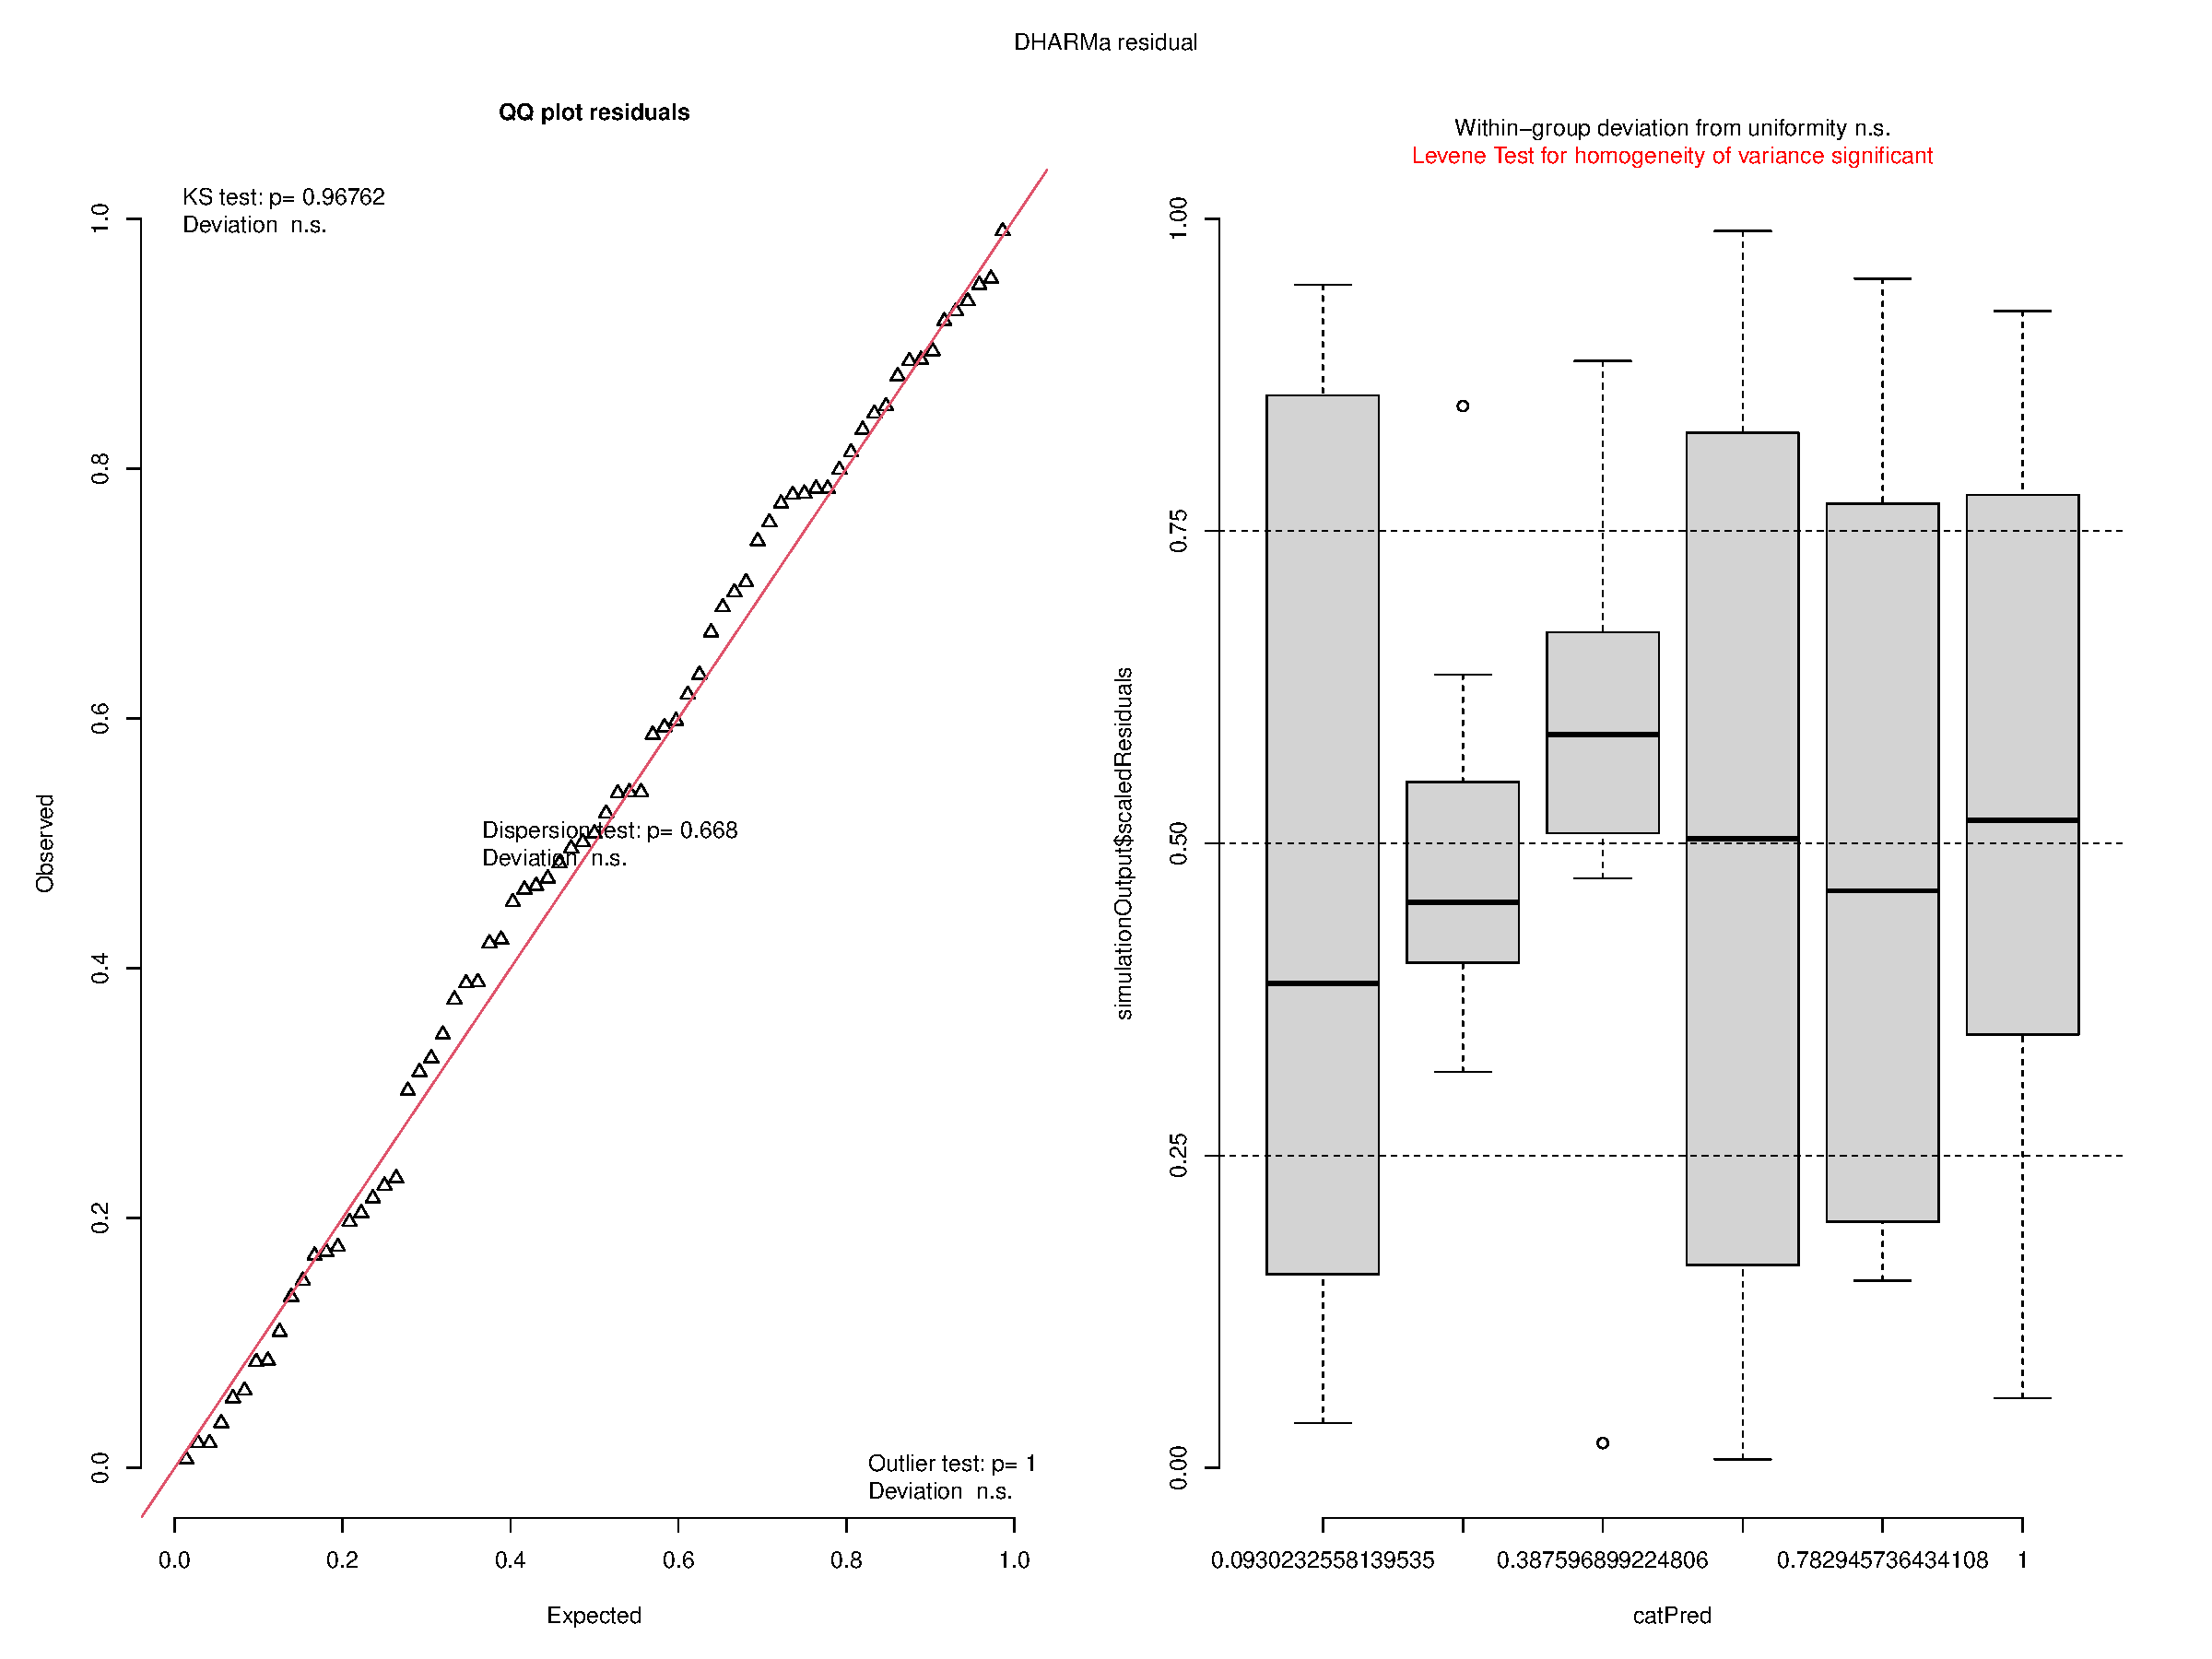
\includegraphics[keepaspectratio]{rsa_day1617_agar_files/figure-pdf/unnamed-chunk-9-6.pdf}}

\begin{Shaded}
\begin{Highlighting}[]
\FunctionTok{testUniformity}\NormalTok{(sim\_res)                     }\CommentTok{\# p \textgreater{} 0.05 = Beta appropriate}
\end{Highlighting}
\end{Shaded}

\pandocbounded{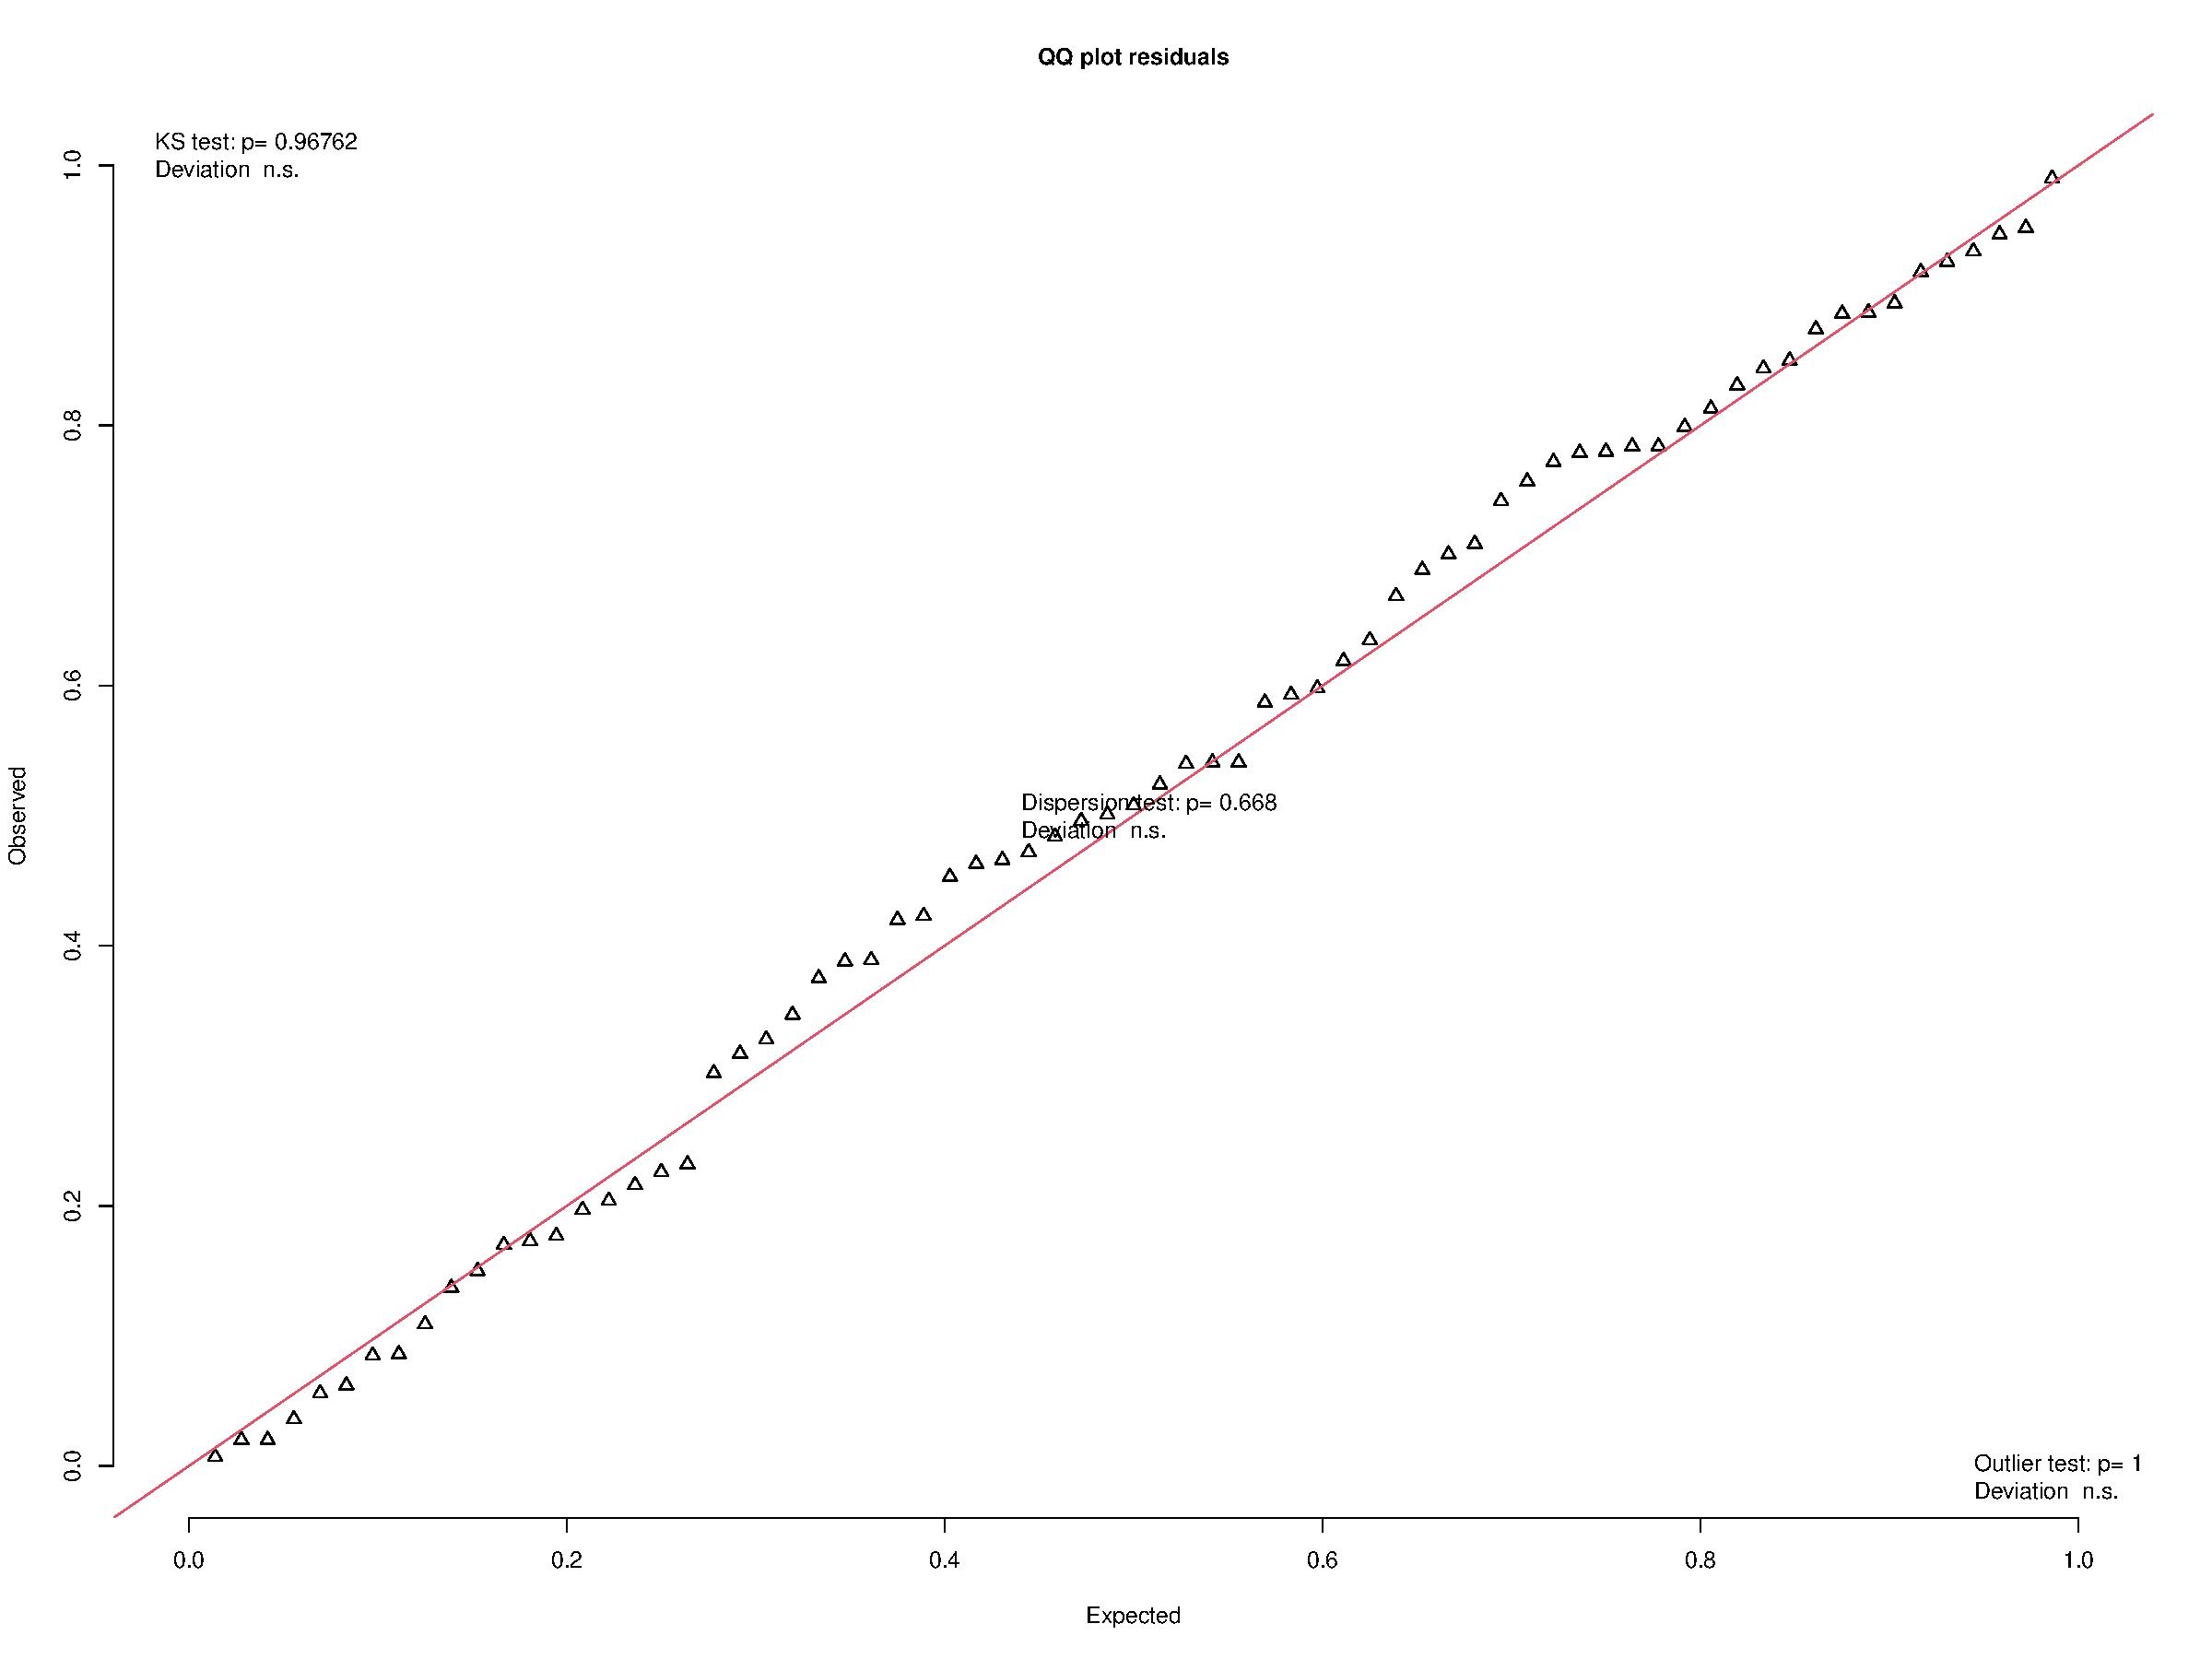
\includegraphics[keepaspectratio]{rsa_day1617_agar_files/figure-pdf/unnamed-chunk-9-7.pdf}}

\begin{verbatim}

    Asymptotic one-sample Kolmogorov-Smirnov test

data:  simulationOutput$scaledResiduals
D = 0.058634, p-value = 0.9676
alternative hypothesis: two-sided
\end{verbatim}

\begin{Shaded}
\begin{Highlighting}[]
\FunctionTok{testDispersion}\NormalTok{(sim\_res)                     }\CommentTok{\# ratio ≈ 1.0}
\end{Highlighting}
\end{Shaded}

\pandocbounded{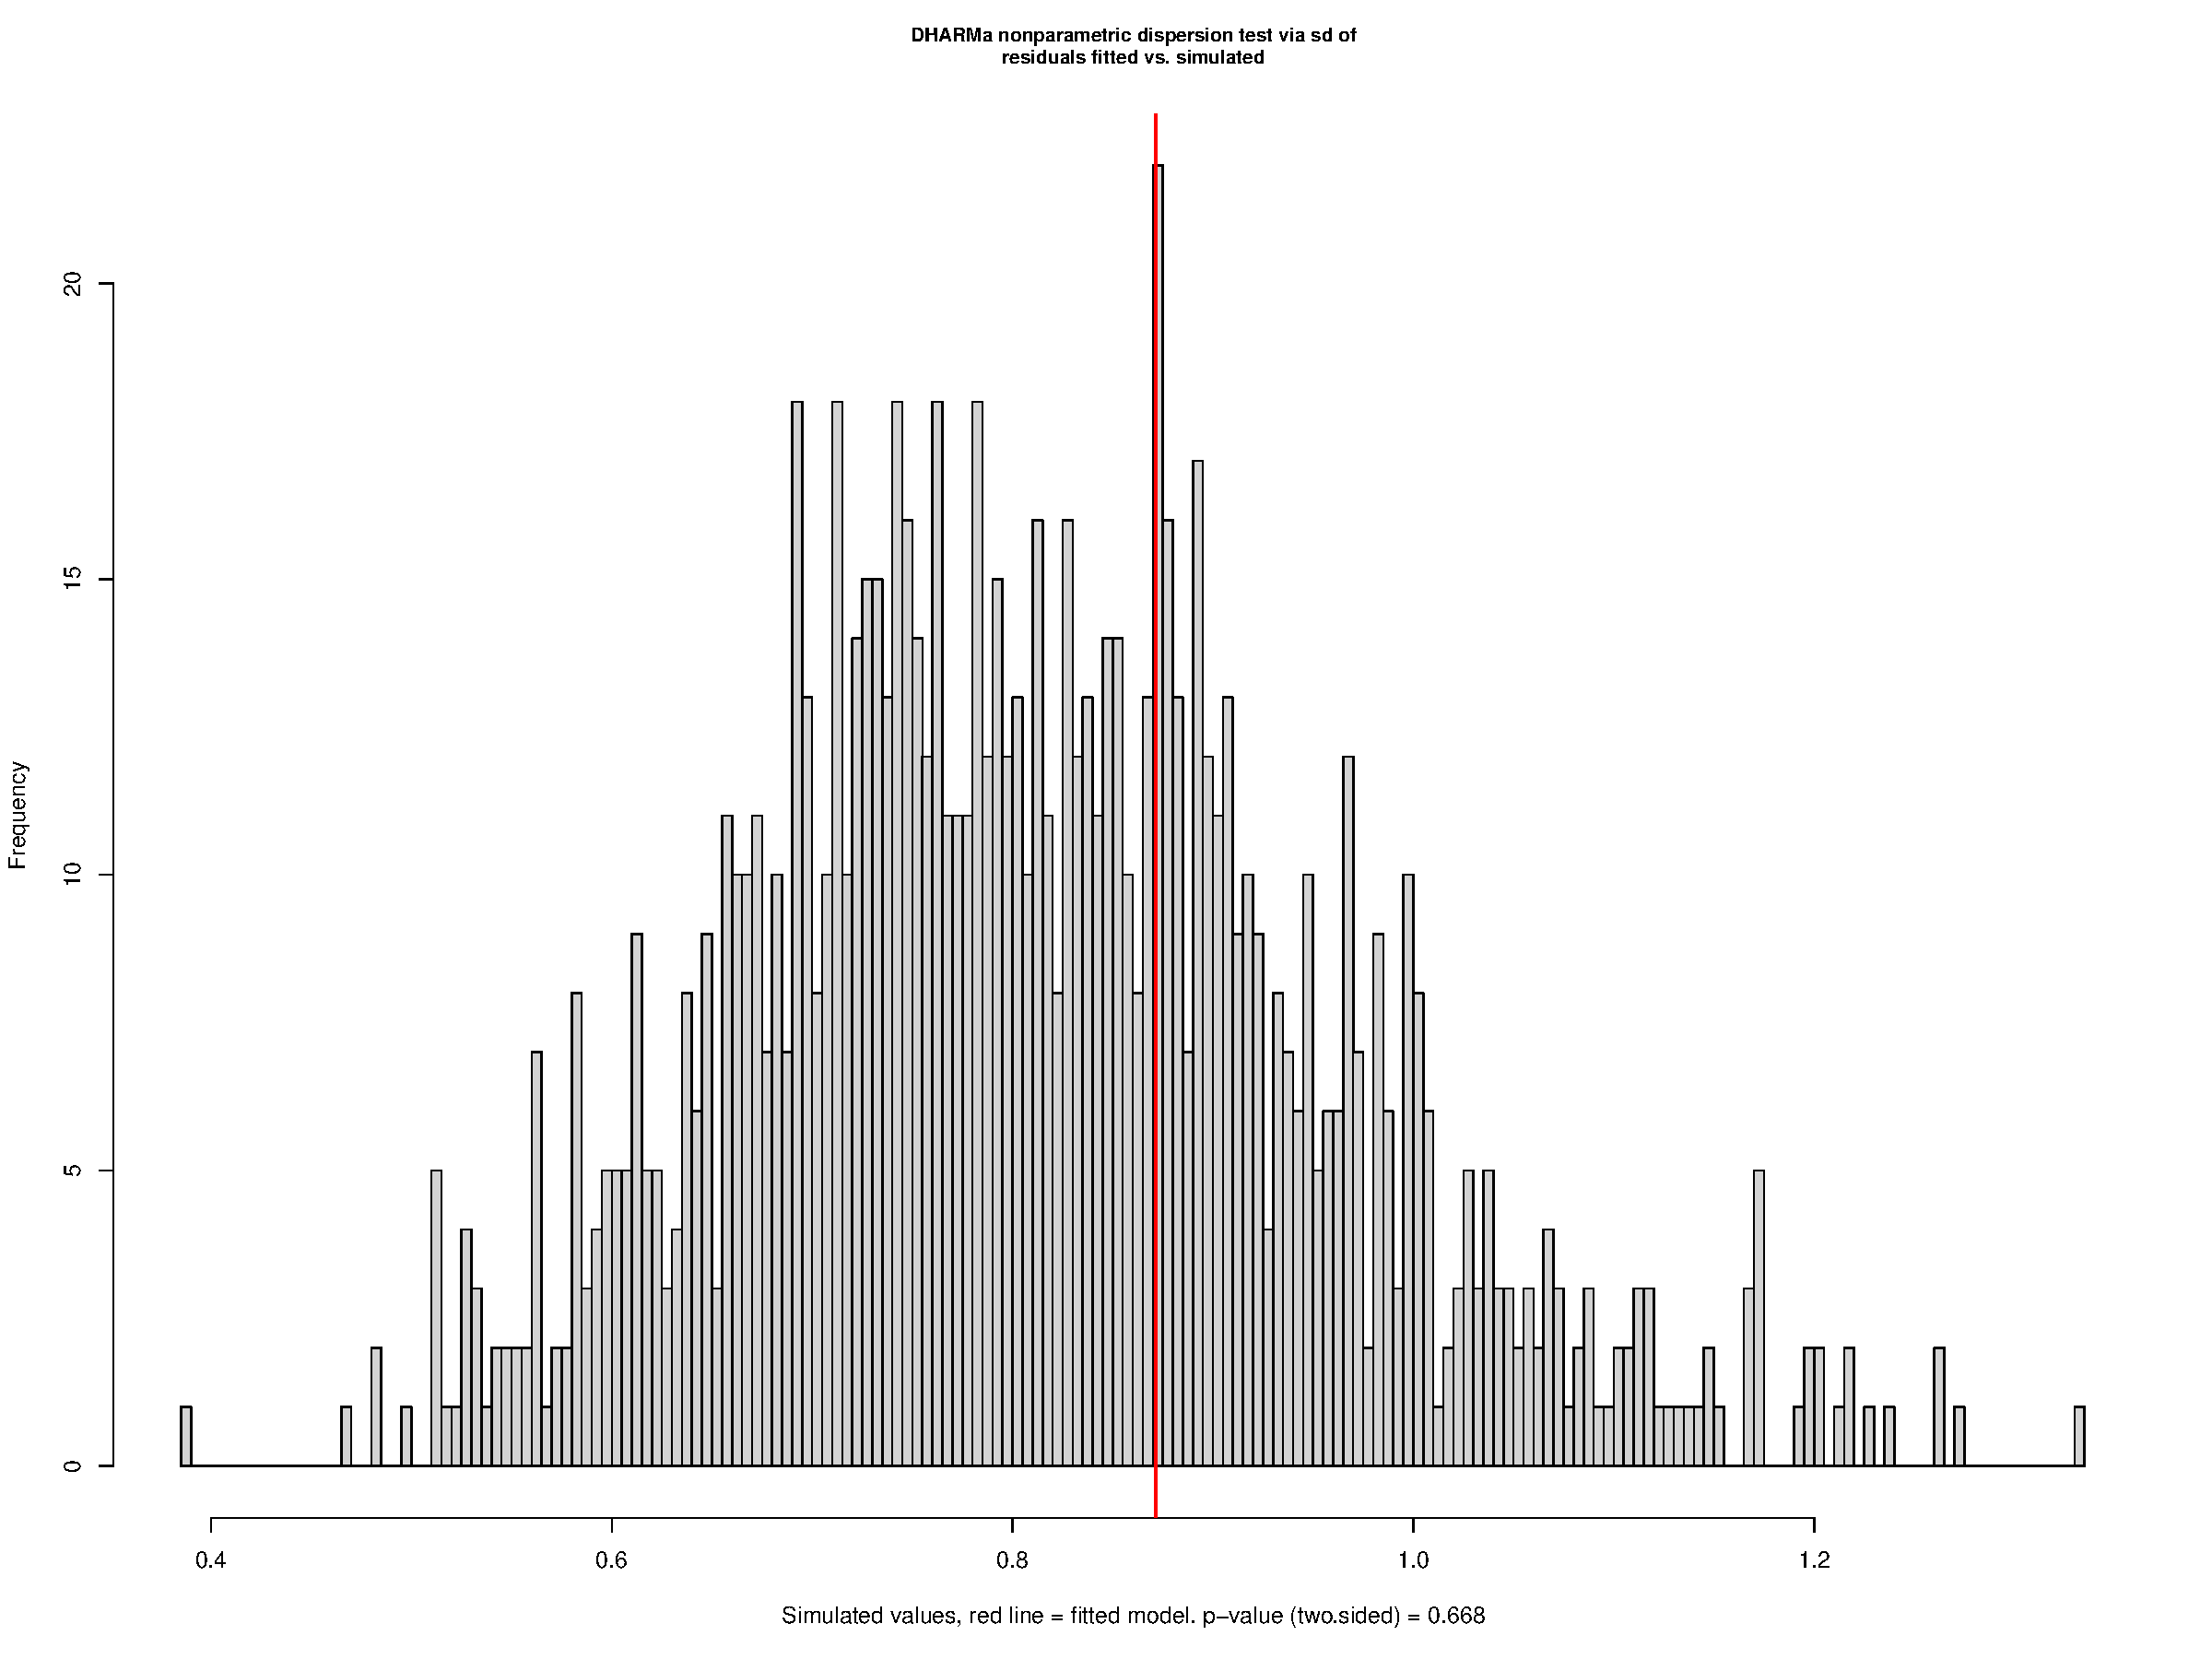
\includegraphics[keepaspectratio]{rsa_day1617_agar_files/figure-pdf/unnamed-chunk-9-8.pdf}}

\begin{verbatim}

    DHARMa nonparametric dispersion test via sd of residuals fitted vs.
    simulated

data:  simulationOutput
dispersion = 1.0705, p-value = 0.668
alternative hypothesis: two.sided
\end{verbatim}

\begin{Shaded}
\begin{Highlighting}[]
\FunctionTok{plotResiduals}\NormalTok{(sim\_res, }\AttributeTok{form =}\NormalTok{ df}\SpecialCharTok{$}\NormalTok{Genotype)  }\CommentTok{\# no patterns per genotype}
\end{Highlighting}
\end{Shaded}

\pandocbounded{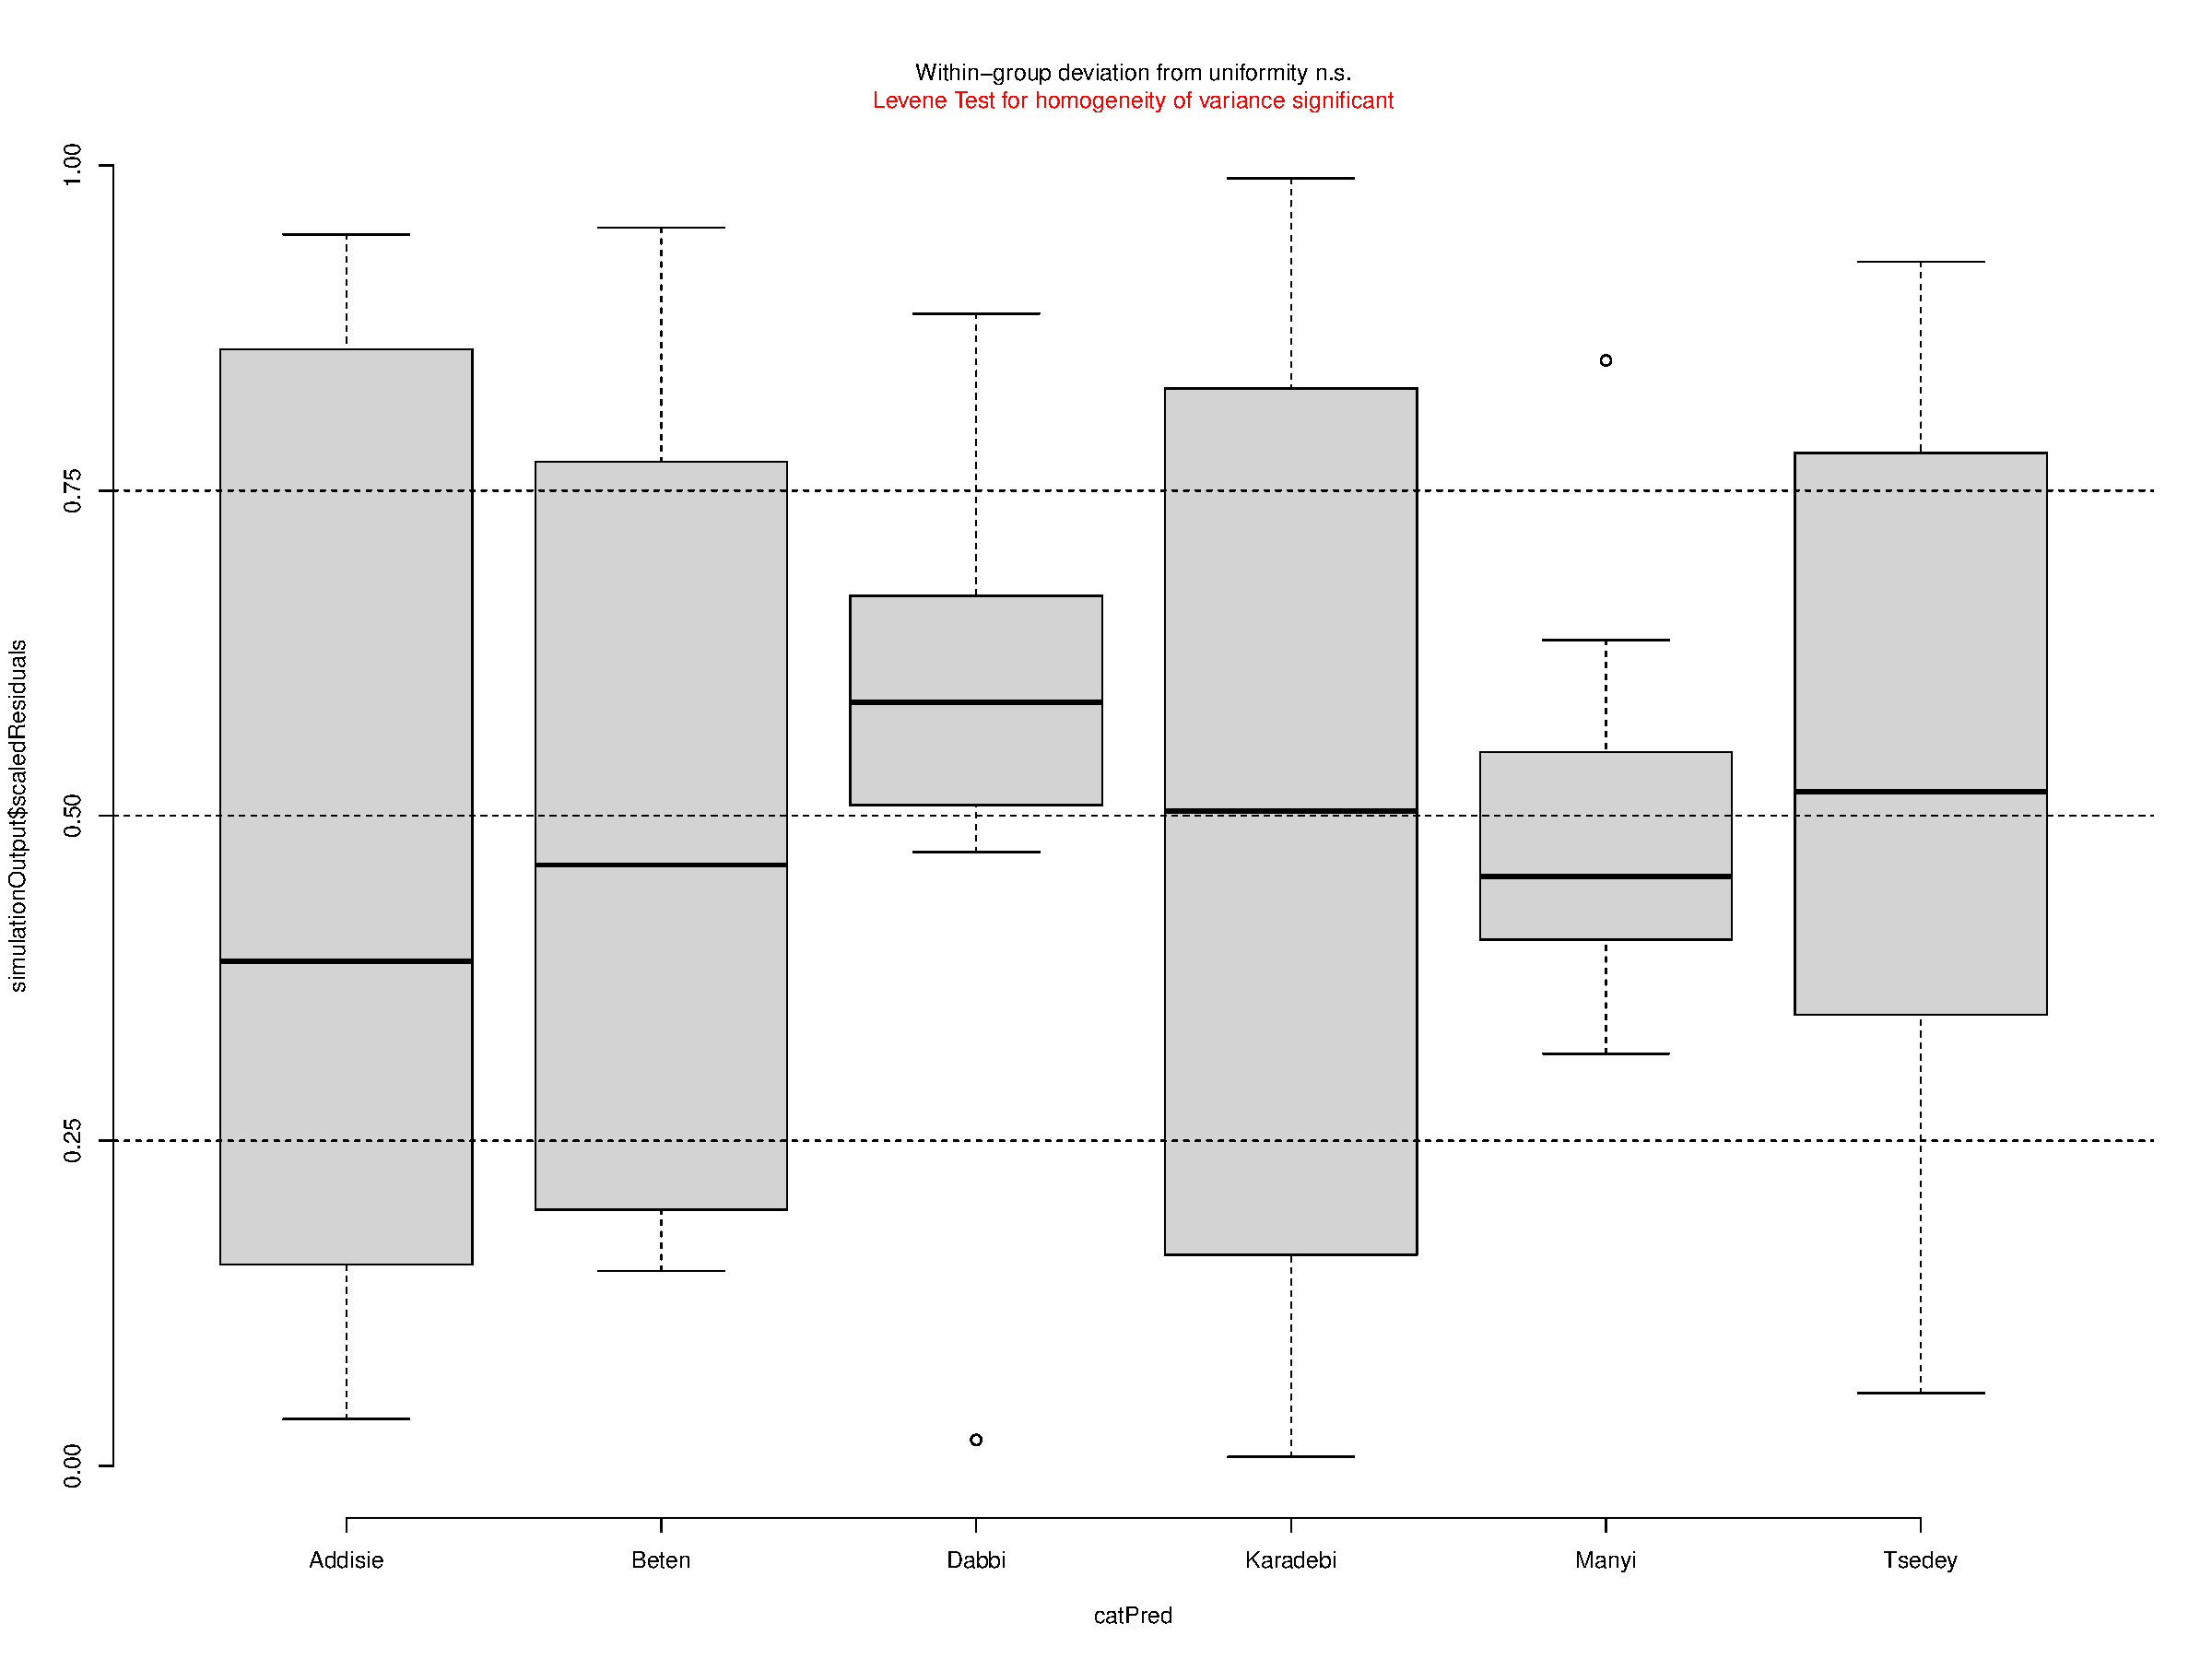
\includegraphics[keepaspectratio]{rsa_day1617_agar_files/figure-pdf/unnamed-chunk-9-9.pdf}}

\begin{Shaded}
\begin{Highlighting}[]
\CommentTok{\# ── 5. Test overall Genotype effect ──────────────────────────}
\NormalTok{car}\SpecialCharTok{::}\FunctionTok{Anova}\NormalTok{(steep\_tmb, }\AttributeTok{type =} \StringTok{"III"}\NormalTok{)}
\end{Highlighting}
\end{Shaded}

\begin{verbatim}
Analysis of Deviance Table (Type III Wald chisquare tests)

Response: Steep.Angle.Frequency
             Chisq Df Pr(>Chisq)    
(Intercept) 39.314  1  3.608e-10 ***
Genotype    17.632  5   0.003445 ** 
---
Signif. codes:  0 '***' 0.001 '**' 0.01 '*' 0.05 '.' 0.1 ' ' 1
\end{verbatim}

\begin{Shaded}
\begin{Highlighting}[]
\CommentTok{\# ── 6. Pairwise comparisons + CLD ────────────────────────────}
\NormalTok{emm }\OtherTok{\textless{}{-}} \FunctionTok{emmeans}\NormalTok{(steep\_tmb, }\SpecialCharTok{\textasciitilde{}}\NormalTok{ Genotype, }\AttributeTok{type =} \StringTok{"response"}\NormalTok{)}
\FunctionTok{pairs}\NormalTok{(emm, }\AttributeTok{adjust =} \StringTok{"sidak"}\NormalTok{)}
\end{Highlighting}
\end{Shaded}

\begin{verbatim}
 contrast           odds.ratio     SE  df null z.ratio p.value
 Addisie / Beten         0.778 0.1730 Inf    1  -1.129  0.9888
 Addisie / Dabbi         0.892 0.1990 Inf    1  -0.511  1.0000
 Addisie / Karadebi      0.840 0.1920 Inf    1  -0.761  0.9999
 Addisie / Manyi         0.994 0.2590 Inf    1  -0.024  1.0000
 Addisie / Tsedey        0.409 0.0989 Inf    1  -3.695  0.0033
 Beten / Dabbi           1.147 0.2470 Inf    1   0.636  1.0000
 Beten / Karadebi        1.080 0.2390 Inf    1   0.347  1.0000
 Beten / Manyi           1.277 0.3240 Inf    1   0.963  0.9978
 Beten / Tsedey          0.526 0.1230 Inf    1  -2.741  0.0881
 Dabbi / Karadebi        0.942 0.2090 Inf    1  -0.270  1.0000
 Dabbi / Manyi           1.114 0.2830 Inf    1   0.423  1.0000
 Dabbi / Tsedey          0.459 0.1080 Inf    1  -3.312  0.0138
 Karadebi / Manyi        1.182 0.3070 Inf    1   0.646  1.0000
 Karadebi / Tsedey       0.487 0.1170 Inf    1  -2.989  0.0412
 Manyi / Tsedey          0.412 0.1120 Inf    1  -3.270  0.0160

P value adjustment: sidak method for 15 tests 
Tests are performed on the log odds ratio scale 
\end{verbatim}

\begin{Shaded}
\begin{Highlighting}[]
\NormalTok{cld\_df }\OtherTok{\textless{}{-}} \FunctionTok{as.data.frame}\NormalTok{(}\FunctionTok{cld}\NormalTok{(emm, }\AttributeTok{adjust =} \StringTok{"sidak"}\NormalTok{,}
                             \AttributeTok{Letters =}\NormalTok{ letters, }\AttributeTok{alpha =} \FloatTok{0.05}\NormalTok{)) }\SpecialCharTok{\%\textgreater{}\%}
  \FunctionTok{mutate}\NormalTok{(}\AttributeTok{.group =} \FunctionTok{trimws}\NormalTok{(.group))}

\FunctionTok{class}\NormalTok{(df}\SpecialCharTok{$}\NormalTok{Genotype)   }\CommentTok{\# should return "factor"}
\end{Highlighting}
\end{Shaded}

\begin{verbatim}
[1] "factor"
\end{verbatim}

\begin{Shaded}
\begin{Highlighting}[]
\FunctionTok{length}\NormalTok{(df}\SpecialCharTok{$}\NormalTok{Genotype)  }\CommentTok{\# should return 71}
\end{Highlighting}
\end{Shaded}

\begin{verbatim}
[1] 71
\end{verbatim}

\begin{Shaded}
\begin{Highlighting}[]
\CommentTok{\# Effect size}

\CommentTok{\# Cohen\textquotesingle{}s d = difference in means / pooled SD}
\CommentTok{\# Interpretation: 0.2 = small, 0.5 = medium, 0.8 = large}

\NormalTok{emm\_steep }\OtherTok{\textless{}{-}} \FunctionTok{emmeans}\NormalTok{(steep\_tmb, }\SpecialCharTok{\textasciitilde{}}\NormalTok{ Genotype)}

\NormalTok{eff\_steep }\OtherTok{\textless{}{-}} \FunctionTok{eff\_size}\NormalTok{(}
\NormalTok{  emm\_steep,}
  \AttributeTok{sigma =} \FunctionTok{sigma}\NormalTok{(steep\_tmb),   }\CommentTok{\# residual SD from model}
  \AttributeTok{edf   =} \FunctionTok{df.residual}\NormalTok{(steep\_tmb)}
\NormalTok{)}
\FunctionTok{print}\NormalTok{(eff\_steep)}
\end{Highlighting}
\end{Shaded}

\begin{verbatim}
 contrast           effect.size     SE  df asymp.LCL asymp.UCL
 Addisie - Beten      -0.015587 0.0139 Inf   -0.0428    0.0116
 Addisie - Dabbi      -0.007081 0.0139 Inf   -0.0343    0.0201
 Addisie - Karadebi   -0.010813 0.0142 Inf   -0.0387    0.0171
 Addisie - Manyi      -0.000392 0.0162 Inf   -0.0321    0.0313
 Addisie - Tsedey     -0.055559 0.0158 Inf   -0.0866   -0.0246
 Beten - Dabbi         0.008506 0.0134 Inf   -0.0178    0.0348
 Beten - Karadebi      0.004775 0.0138 Inf   -0.0222    0.0317
 Beten - Manyi         0.015196 0.0158 Inf   -0.0159    0.0462
 Beten - Tsedey       -0.039971 0.0150 Inf   -0.0694   -0.0106
 Dabbi - Karadebi     -0.003731 0.0138 Inf   -0.0308    0.0233
 Dabbi - Manyi         0.006690 0.0158 Inf   -0.0243    0.0377
 Dabbi - Tsedey       -0.048477 0.0153 Inf   -0.0784   -0.0186
 Karadebi - Manyi      0.010421 0.0162 Inf   -0.0213    0.0421
 Karadebi - Tsedey    -0.044746 0.0155 Inf   -0.0751   -0.0144
 Manyi - Tsedey       -0.055167 0.0176 Inf   -0.0896   -0.0208

sigma used for effect sizes: 16.08 
Confidence level used: 0.95 
\end{verbatim}

\begin{Shaded}
\begin{Highlighting}[]
\CommentTok{\# ── 7. Plot 1 — Boxplot ───────────────────────────────────────}

\NormalTok{y\_ceil }\OtherTok{\textless{}{-}} \FunctionTok{max}\NormalTok{(df}\SpecialCharTok{$}\NormalTok{Steep.Angle.Frequency) }\SpecialCharTok{*} \FloatTok{1.22}
\NormalTok{y\_label }\OtherTok{\textless{}{-}}\NormalTok{ y\_ceil }\SpecialCharTok{*} \FloatTok{0.95}

\NormalTok{p1 }\OtherTok{\textless{}{-}} \FunctionTok{ggplot}\NormalTok{(df, }\FunctionTok{aes}\NormalTok{(}\AttributeTok{x =}\NormalTok{ Genotype, }\AttributeTok{y =}\NormalTok{ Steep.Angle.Frequency, }\AttributeTok{fill =}\NormalTok{ Genotype)) }\SpecialCharTok{+}

  \FunctionTok{geom\_boxplot}\NormalTok{(}
    \AttributeTok{alpha         =} \FloatTok{0.7}\NormalTok{,}
    \AttributeTok{outlier.shape =} \ConstantTok{NA}\NormalTok{,}
    \AttributeTok{width         =} \FloatTok{0.5}\NormalTok{,}
    \AttributeTok{colour        =} \StringTok{"black"}\NormalTok{,}
    \AttributeTok{linewidth     =} \FloatTok{0.5}
\NormalTok{  ) }\SpecialCharTok{+}

  \FunctionTok{geom\_jitter}\NormalTok{(}
    \AttributeTok{width  =} \FloatTok{0.15}\NormalTok{,}
    \AttributeTok{size   =} \FloatTok{1.8}\NormalTok{,}
    \AttributeTok{alpha  =} \FloatTok{0.55}\NormalTok{,}
    \AttributeTok{colour =} \StringTok{"black"}
\NormalTok{  ) }\SpecialCharTok{+}

  \FunctionTok{geom\_text}\NormalTok{(}
    \AttributeTok{data        =}\NormalTok{ cld\_df,}
    \FunctionTok{aes}\NormalTok{(}\AttributeTok{x =}\NormalTok{ Genotype, }\AttributeTok{label =}\NormalTok{ .group),}
    \AttributeTok{y           =}\NormalTok{ y\_label,}
    \AttributeTok{inherit.aes =} \ConstantTok{FALSE}\NormalTok{,}
    \AttributeTok{size        =} \DecValTok{5}\NormalTok{,}
    \AttributeTok{fontface    =} \StringTok{"bold"}\NormalTok{,}
    \AttributeTok{colour      =} \StringTok{"grey20"}
\NormalTok{  ) }\SpecialCharTok{+}

  \FunctionTok{geom\_text}\NormalTok{(}
    \AttributeTok{data        =}\NormalTok{ n\_df,}
    \FunctionTok{aes}\NormalTok{(}\AttributeTok{x =}\NormalTok{ Genotype, }\AttributeTok{label =}\NormalTok{ label),}
    \AttributeTok{y           =} \SpecialCharTok{{-}}\ConstantTok{Inf}\NormalTok{,}
    \AttributeTok{vjust       =} \FloatTok{4.2}\NormalTok{,}
    \AttributeTok{inherit.aes =} \ConstantTok{FALSE}\NormalTok{,}
    \AttributeTok{size        =} \FloatTok{3.5}\NormalTok{,}
    \AttributeTok{colour      =} \StringTok{"grey40"}
\NormalTok{  ) }\SpecialCharTok{+}

  \FunctionTok{scale\_fill\_brewer}\NormalTok{(}\AttributeTok{palette =} \StringTok{"Set2"}\NormalTok{) }\SpecialCharTok{+}

  \FunctionTok{labs}\NormalTok{(}
    \AttributeTok{x       =} \StringTok{"Genotype"}\NormalTok{,}
    \AttributeTok{y       =} \StringTok{"Steep angle frequency"}\NormalTok{,}
    \AttributeTok{caption =} \StringTok{"Shared letters indicate no significant difference (sidak HSD, p \textgreater{} 0.05; glmmTMB, Beta)"}
\NormalTok{  ) }\SpecialCharTok{+}

  \FunctionTok{theme\_classic}\NormalTok{(}\AttributeTok{base\_size =} \DecValTok{14}\NormalTok{) }\SpecialCharTok{+}
  \FunctionTok{theme}\NormalTok{(}
    \AttributeTok{legend.position =} \StringTok{"none"}\NormalTok{,}
    \AttributeTok{axis.line       =} \FunctionTok{element\_line}\NormalTok{(}\AttributeTok{colour =} \StringTok{"black"}\NormalTok{, }\AttributeTok{linewidth =} \FloatTok{0.6}\NormalTok{),}
    \AttributeTok{axis.ticks      =} \FunctionTok{element\_line}\NormalTok{(}\AttributeTok{colour =} \StringTok{"black"}\NormalTok{, }\AttributeTok{linewidth =} \FloatTok{0.5}\NormalTok{),}
    \AttributeTok{axis.title      =} \FunctionTok{element\_text}\NormalTok{(}\AttributeTok{size =} \DecValTok{14}\NormalTok{, }\AttributeTok{face =} \StringTok{"bold"}\NormalTok{),}
    \AttributeTok{axis.text       =} \FunctionTok{element\_text}\NormalTok{(}\AttributeTok{size =} \DecValTok{14}\NormalTok{, }\AttributeTok{colour =} \StringTok{"black"}\NormalTok{),}
    \AttributeTok{axis.text.x     =} \FunctionTok{element\_text}\NormalTok{(}\AttributeTok{face =} \StringTok{"italic"}\NormalTok{, }\AttributeTok{margin =} \FunctionTok{margin}\NormalTok{(}\AttributeTok{t =} \DecValTok{3}\NormalTok{)),}
    \AttributeTok{plot.caption    =} \FunctionTok{element\_text}\NormalTok{(}\AttributeTok{size =} \DecValTok{9}\NormalTok{, }\AttributeTok{colour =} \StringTok{"grey40"}\NormalTok{, }\AttributeTok{hjust =} \DecValTok{0}\NormalTok{),}
    \AttributeTok{plot.margin     =} \FunctionTok{margin}\NormalTok{(}\AttributeTok{t =} \DecValTok{10}\NormalTok{, }\AttributeTok{r =} \DecValTok{15}\NormalTok{, }\AttributeTok{b =} \DecValTok{30}\NormalTok{, }\AttributeTok{l =} \DecValTok{10}\NormalTok{)}
\NormalTok{  )}

\NormalTok{p1 }\SpecialCharTok{+} \FunctionTok{coord\_cartesian}\NormalTok{(}
  \AttributeTok{ylim =} \FunctionTok{c}\NormalTok{(}\DecValTok{0}\NormalTok{, }\FunctionTok{max}\NormalTok{(df}\SpecialCharTok{$}\NormalTok{Steep.Angle.Frequency) }\SpecialCharTok{*} \FloatTok{1.22}\NormalTok{),}
  \AttributeTok{clip =} \StringTok{"off"}
\NormalTok{)}
\end{Highlighting}
\end{Shaded}

\pandocbounded{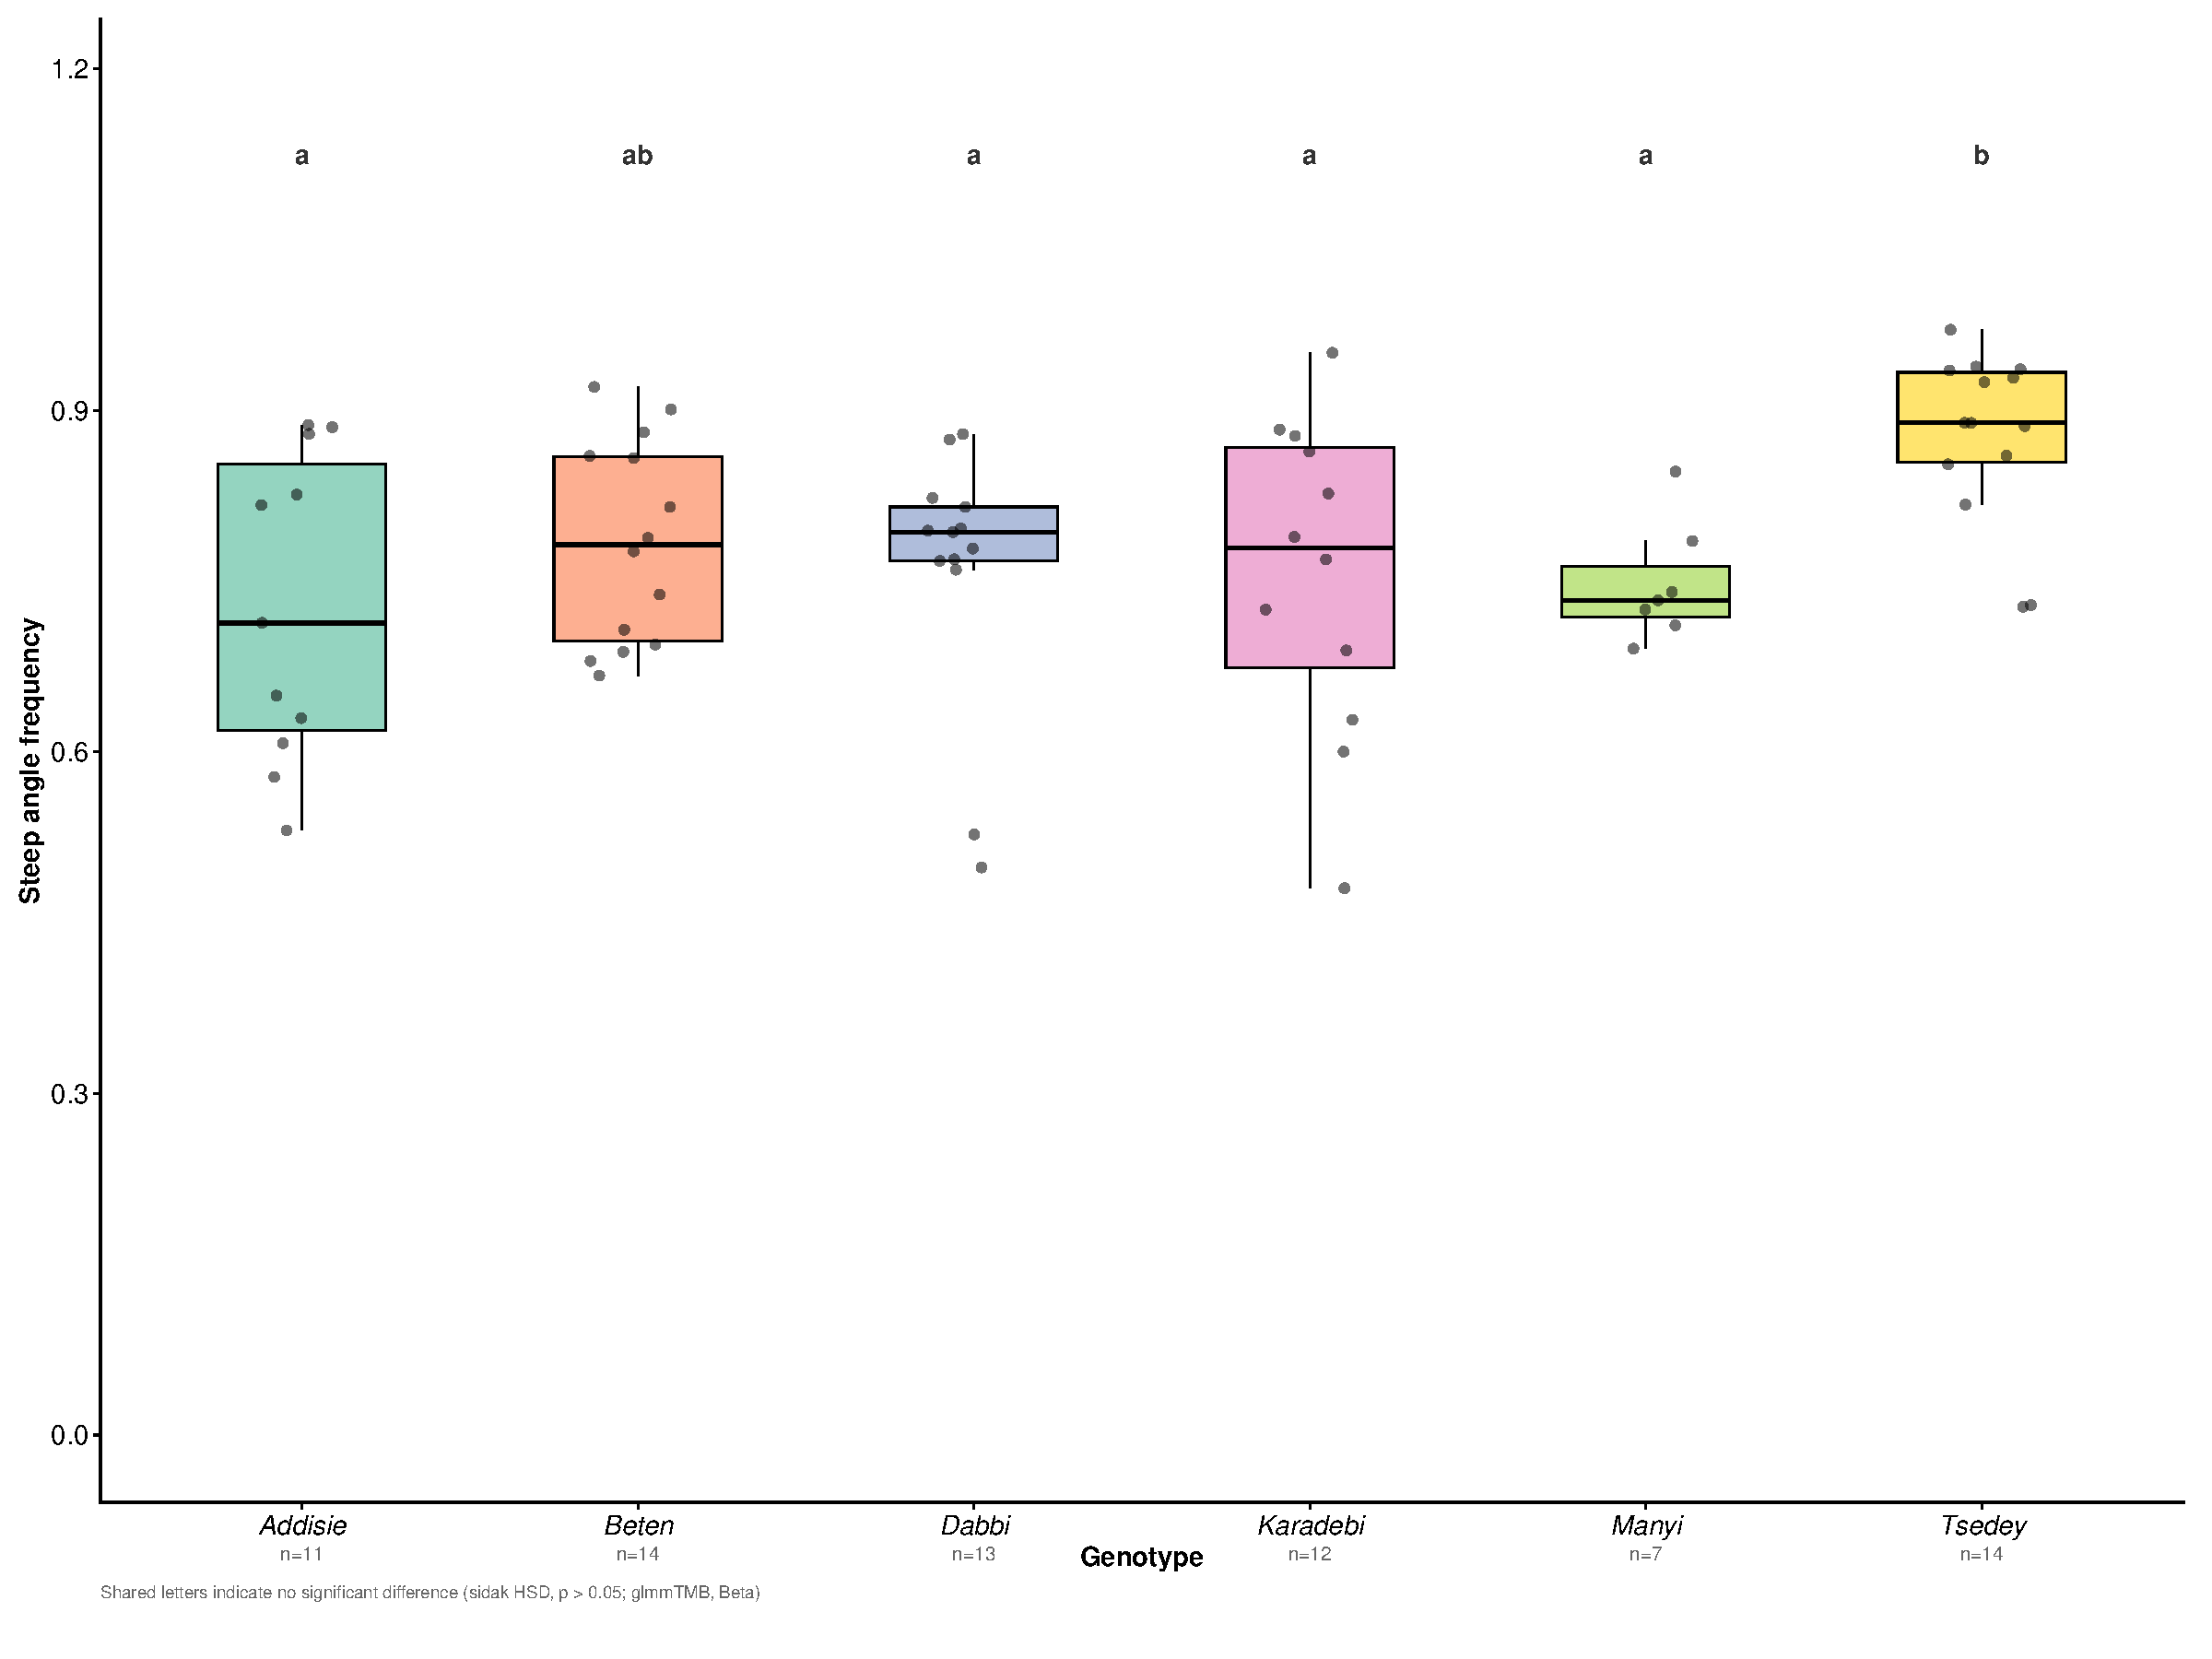
\includegraphics[keepaspectratio]{rsa_day1617_agar_files/figure-pdf/unnamed-chunk-9-10.pdf}}

\begin{Shaded}
\begin{Highlighting}[]
\CommentTok{\# full model}

\CommentTok{\# ── 6. Pairwise comparisons + CLD ────────────────────────────}
\NormalTok{emm }\OtherTok{\textless{}{-}} \FunctionTok{emmeans}\NormalTok{(steep\_full, }\SpecialCharTok{\textasciitilde{}}\NormalTok{ Genotype, }\AttributeTok{type =} \StringTok{"response"}\NormalTok{)}
\FunctionTok{pairs}\NormalTok{(emm, }\AttributeTok{adjust =} \StringTok{"sidak"}\NormalTok{)}
\end{Highlighting}
\end{Shaded}

\begin{verbatim}
 contrast           odds.ratio     SE  df null z.ratio p.value
 Addisie / Beten         0.775 0.1670 Inf    1  -1.179  0.9832
 Addisie / Dabbi         0.835 0.2040 Inf    1  -0.738  0.9999
 Addisie / Karadebi      0.851 0.1950 Inf    1  -0.706  0.9999
 Addisie / Manyi         1.000 0.2660 Inf    1  -0.001  1.0000
 Addisie / Tsedey        0.404 0.0977 Inf    1  -3.747  0.0027
 Beten / Dabbi           1.077 0.2530 Inf    1   0.315  1.0000
 Beten / Karadebi        1.097 0.2440 Inf    1   0.417  1.0000
 Beten / Manyi           1.290 0.3310 Inf    1   0.991  0.9970
 Beten / Tsedey          0.521 0.1220 Inf    1  -2.772  0.0803
 Dabbi / Karadebi        1.019 0.2390 Inf    1   0.080  1.0000
 Dabbi / Manyi           1.198 0.3240 Inf    1   0.666  1.0000
 Dabbi / Tsedey          0.484 0.1240 Inf    1  -2.840  0.0656
 Karadebi / Manyi        1.175 0.3020 Inf    1   0.628  1.0000
 Karadebi / Tsedey       0.475 0.1170 Inf    1  -3.033  0.0357
 Manyi / Tsedey          0.404 0.1110 Inf    1  -3.303  0.0143

P value adjustment: sidak method for 15 tests 
Tests are performed on the log odds ratio scale 
\end{verbatim}

\begin{Shaded}
\begin{Highlighting}[]
\NormalTok{cld\_df }\OtherTok{\textless{}{-}} \FunctionTok{as.data.frame}\NormalTok{(}\FunctionTok{cld}\NormalTok{(emm, }\AttributeTok{adjust =} \StringTok{"sidak"}\NormalTok{,}
                             \AttributeTok{Letters =}\NormalTok{ letters, }\AttributeTok{alpha =} \FloatTok{0.05}\NormalTok{)) }\SpecialCharTok{\%\textgreater{}\%}
  \FunctionTok{mutate}\NormalTok{(}\AttributeTok{.group =} \FunctionTok{trimws}\NormalTok{(.group))}

\CommentTok{\# Effect size}

\CommentTok{\# Cohen\textquotesingle{}s d = difference in means / pooled SD}
\CommentTok{\# Interpretation: 0.2 = small, 0.5 = medium, 0.8 = large}

\NormalTok{emm\_steep }\OtherTok{\textless{}{-}} \FunctionTok{emmeans}\NormalTok{(steep\_full, }\SpecialCharTok{\textasciitilde{}}\NormalTok{ Genotype)}

\NormalTok{eff\_steep }\OtherTok{\textless{}{-}} \FunctionTok{eff\_size}\NormalTok{(}
\NormalTok{  emm\_steep,}
  \AttributeTok{sigma =} \FunctionTok{sigma}\NormalTok{(steep\_full),   }\CommentTok{\# residual SD from model}
  \AttributeTok{edf   =} \FunctionTok{df.residual}\NormalTok{(steep\_full)}
\NormalTok{) }
\FunctionTok{print}\NormalTok{(eff\_steep)}
\end{Highlighting}
\end{Shaded}

\begin{verbatim}
 contrast           effect.size     SE  df asymp.LCL asymp.UCL
 Addisie - Beten      -1.43e-02 0.0122 Inf   -0.0382   0.00961
 Addisie - Dabbi      -1.01e-02 0.0138 Inf   -0.0371   0.01684
 Addisie - Karadebi   -9.08e-03 0.0129 Inf   -0.0344   0.01620
 Addisie - Manyi      -1.34e-05 0.0149 Inf   -0.0293   0.02924
 Addisie - Tsedey     -5.09e-02 0.0143 Inf   -0.0790  -0.02277
 Beten - Dabbi         4.16e-03 0.0132 Inf   -0.0217   0.03003
 Beten - Karadebi      5.22e-03 0.0125 Inf   -0.0193   0.02976
 Beten - Manyi         1.43e-02 0.0145 Inf   -0.0141   0.04265
 Beten - Tsedey       -3.66e-02 0.0136 Inf   -0.0632  -0.00992
 Dabbi - Karadebi      1.06e-03 0.0132 Inf   -0.0248   0.02689
 Dabbi - Manyi         1.01e-02 0.0152 Inf   -0.0197   0.03998
 Dabbi - Tsedey       -4.07e-02 0.0148 Inf   -0.0698  -0.01171
 Karadebi - Manyi      9.07e-03 0.0145 Inf   -0.0193   0.03740
 Karadebi - Tsedey    -4.18e-02 0.0143 Inf   -0.0698  -0.01379
 Manyi - Tsedey       -5.09e-02 0.0161 Inf   -0.0824  -0.01936

sigma used for effect sizes: 17.8 
Confidence level used: 0.95 
\end{verbatim}

\begin{Shaded}
\begin{Highlighting}[]
\CommentTok{\# ── 7. Plot 1 — Boxplot ───────────────────────────────────────}

\NormalTok{y\_ceil }\OtherTok{\textless{}{-}} \FunctionTok{max}\NormalTok{(df}\SpecialCharTok{$}\NormalTok{Steep.Angle.Frequency) }\SpecialCharTok{*} \FloatTok{1.22}
\NormalTok{y\_label }\OtherTok{\textless{}{-}}\NormalTok{ y\_ceil }\SpecialCharTok{*} \FloatTok{0.95}

\NormalTok{p1 }\OtherTok{\textless{}{-}} \FunctionTok{ggplot}\NormalTok{(df, }\FunctionTok{aes}\NormalTok{(}\AttributeTok{x =}\NormalTok{ Genotype, }\AttributeTok{y =}\NormalTok{ Steep.Angle.Frequency, }\AttributeTok{fill =}\NormalTok{ Genotype)) }\SpecialCharTok{+}

  \FunctionTok{geom\_boxplot}\NormalTok{(}
    \AttributeTok{alpha         =} \FloatTok{0.7}\NormalTok{,}
    \AttributeTok{outlier.shape =} \ConstantTok{NA}\NormalTok{,}
    \AttributeTok{width         =} \FloatTok{0.5}\NormalTok{,}
    \AttributeTok{colour        =} \StringTok{"black"}\NormalTok{,}
    \AttributeTok{linewidth     =} \FloatTok{0.5}
\NormalTok{  ) }\SpecialCharTok{+}

  \FunctionTok{geom\_jitter}\NormalTok{(}
    \AttributeTok{width  =} \FloatTok{0.15}\NormalTok{,}
    \AttributeTok{size   =} \FloatTok{1.8}\NormalTok{,}
    \AttributeTok{alpha  =} \FloatTok{0.55}\NormalTok{,}
    \AttributeTok{colour =} \StringTok{"black"}
\NormalTok{  ) }\SpecialCharTok{+}

  \FunctionTok{geom\_text}\NormalTok{(}
    \AttributeTok{data        =}\NormalTok{ cld\_df,}
    \FunctionTok{aes}\NormalTok{(}\AttributeTok{x =}\NormalTok{ Genotype, }\AttributeTok{label =}\NormalTok{ .group),}
    \AttributeTok{y           =}\NormalTok{ y\_label,}
    \AttributeTok{inherit.aes =} \ConstantTok{FALSE}\NormalTok{,}
    \AttributeTok{size        =} \DecValTok{8}\NormalTok{,}
    \AttributeTok{fontface    =} \StringTok{"bold"}\NormalTok{,}
    \AttributeTok{colour      =} \StringTok{"grey20"}
\NormalTok{  ) }\SpecialCharTok{+}

  \FunctionTok{geom\_text}\NormalTok{(}
    \AttributeTok{data        =}\NormalTok{ n\_df,}
    \FunctionTok{aes}\NormalTok{(}\AttributeTok{x =}\NormalTok{ Genotype, }\AttributeTok{label =}\NormalTok{ label),}
    \AttributeTok{y           =} \SpecialCharTok{{-}}\ConstantTok{Inf}\NormalTok{,}
    \AttributeTok{vjust       =} \FloatTok{4.2}\NormalTok{,}
    \AttributeTok{inherit.aes =} \ConstantTok{FALSE}\NormalTok{,}
    \AttributeTok{size        =} \DecValTok{6}\NormalTok{,}
    \AttributeTok{colour      =} \StringTok{"grey40"}
\NormalTok{  ) }\SpecialCharTok{+}

  \FunctionTok{scale\_fill\_brewer}\NormalTok{(}\AttributeTok{palette =} \StringTok{"Set2"}\NormalTok{) }\SpecialCharTok{+}

  \FunctionTok{labs}\NormalTok{(}
    \AttributeTok{x       =} \StringTok{"Genotype"}\NormalTok{,}
    \AttributeTok{y       =} \StringTok{"Steep angle frequency"}\NormalTok{,}
    \AttributeTok{caption =} \StringTok{"Shared letters indicate no significant difference (sidak HSD, p \textgreater{} 0.05; glmmTMB, Beta)"}
\NormalTok{  ) }\SpecialCharTok{+}

  \FunctionTok{theme\_classic}\NormalTok{(}\AttributeTok{base\_size =} \DecValTok{14}\NormalTok{) }\SpecialCharTok{+}
  \FunctionTok{theme}\NormalTok{(}
    \AttributeTok{legend.position =} \StringTok{"none"}\NormalTok{,}
    \AttributeTok{panel.grid      =} \FunctionTok{element\_blank}\NormalTok{(),}
    \AttributeTok{axis.line       =} \FunctionTok{element\_line}\NormalTok{(}\AttributeTok{colour =} \StringTok{"black"}\NormalTok{, }\AttributeTok{linewidth =} \FloatTok{0.6}\NormalTok{),}
    \AttributeTok{axis.ticks      =} \FunctionTok{element\_line}\NormalTok{(}\AttributeTok{colour =} \StringTok{"black"}\NormalTok{, }\AttributeTok{linewidth =} \FloatTok{0.5}\NormalTok{),}
    \AttributeTok{axis.title      =} \FunctionTok{element\_text}\NormalTok{(}\AttributeTok{size =} \DecValTok{26}\NormalTok{, }\AttributeTok{face =} \StringTok{"bold"}\NormalTok{),}
    \AttributeTok{axis.title.x    =} \FunctionTok{element\_text}\NormalTok{(}\AttributeTok{size =} \DecValTok{26}\NormalTok{, }\AttributeTok{face =} \StringTok{"bold"}\NormalTok{, }\AttributeTok{margin =} \FunctionTok{margin}\NormalTok{(}\AttributeTok{t =} \DecValTok{24}\NormalTok{)),}
    \AttributeTok{axis.text       =} \FunctionTok{element\_text}\NormalTok{(}\AttributeTok{size =} \DecValTok{22}\NormalTok{, }\AttributeTok{colour =} \StringTok{"black"}\NormalTok{),}
    \AttributeTok{axis.text.x     =} \FunctionTok{element\_text}\NormalTok{(}\AttributeTok{face =} \StringTok{"italic"}\NormalTok{, }\AttributeTok{margin =} \FunctionTok{margin}\NormalTok{(}\AttributeTok{t =} \DecValTok{15}\NormalTok{)),}
    \AttributeTok{plot.caption    =} \FunctionTok{element\_text}\NormalTok{(}\AttributeTok{size =} \DecValTok{12}\NormalTok{, }\AttributeTok{colour =} \StringTok{"grey40"}\NormalTok{, }\AttributeTok{hjust =} \DecValTok{0}\NormalTok{, }\AttributeTok{margin =} \FunctionTok{margin}\NormalTok{(}\AttributeTok{t =} \DecValTok{10}\NormalTok{)),}
    \AttributeTok{plot.margin     =} \FunctionTok{margin}\NormalTok{(}\AttributeTok{t =} \DecValTok{25}\NormalTok{, }\AttributeTok{r =} \DecValTok{25}\NormalTok{, }\AttributeTok{b =} \DecValTok{25}\NormalTok{, }\AttributeTok{l =} \DecValTok{25}\NormalTok{)}
\NormalTok{  )}


\NormalTok{p1 }\SpecialCharTok{+} \FunctionTok{coord\_cartesian}\NormalTok{(}
  \AttributeTok{ylim =} \FunctionTok{c}\NormalTok{(}\DecValTok{0}\NormalTok{, }\FunctionTok{max}\NormalTok{(df}\SpecialCharTok{$}\NormalTok{Steep.Angle.Frequency) }\SpecialCharTok{*} \FloatTok{1.22}\NormalTok{),}
  \AttributeTok{clip =} \StringTok{"off"}
\NormalTok{)}
\end{Highlighting}
\end{Shaded}

\pandocbounded{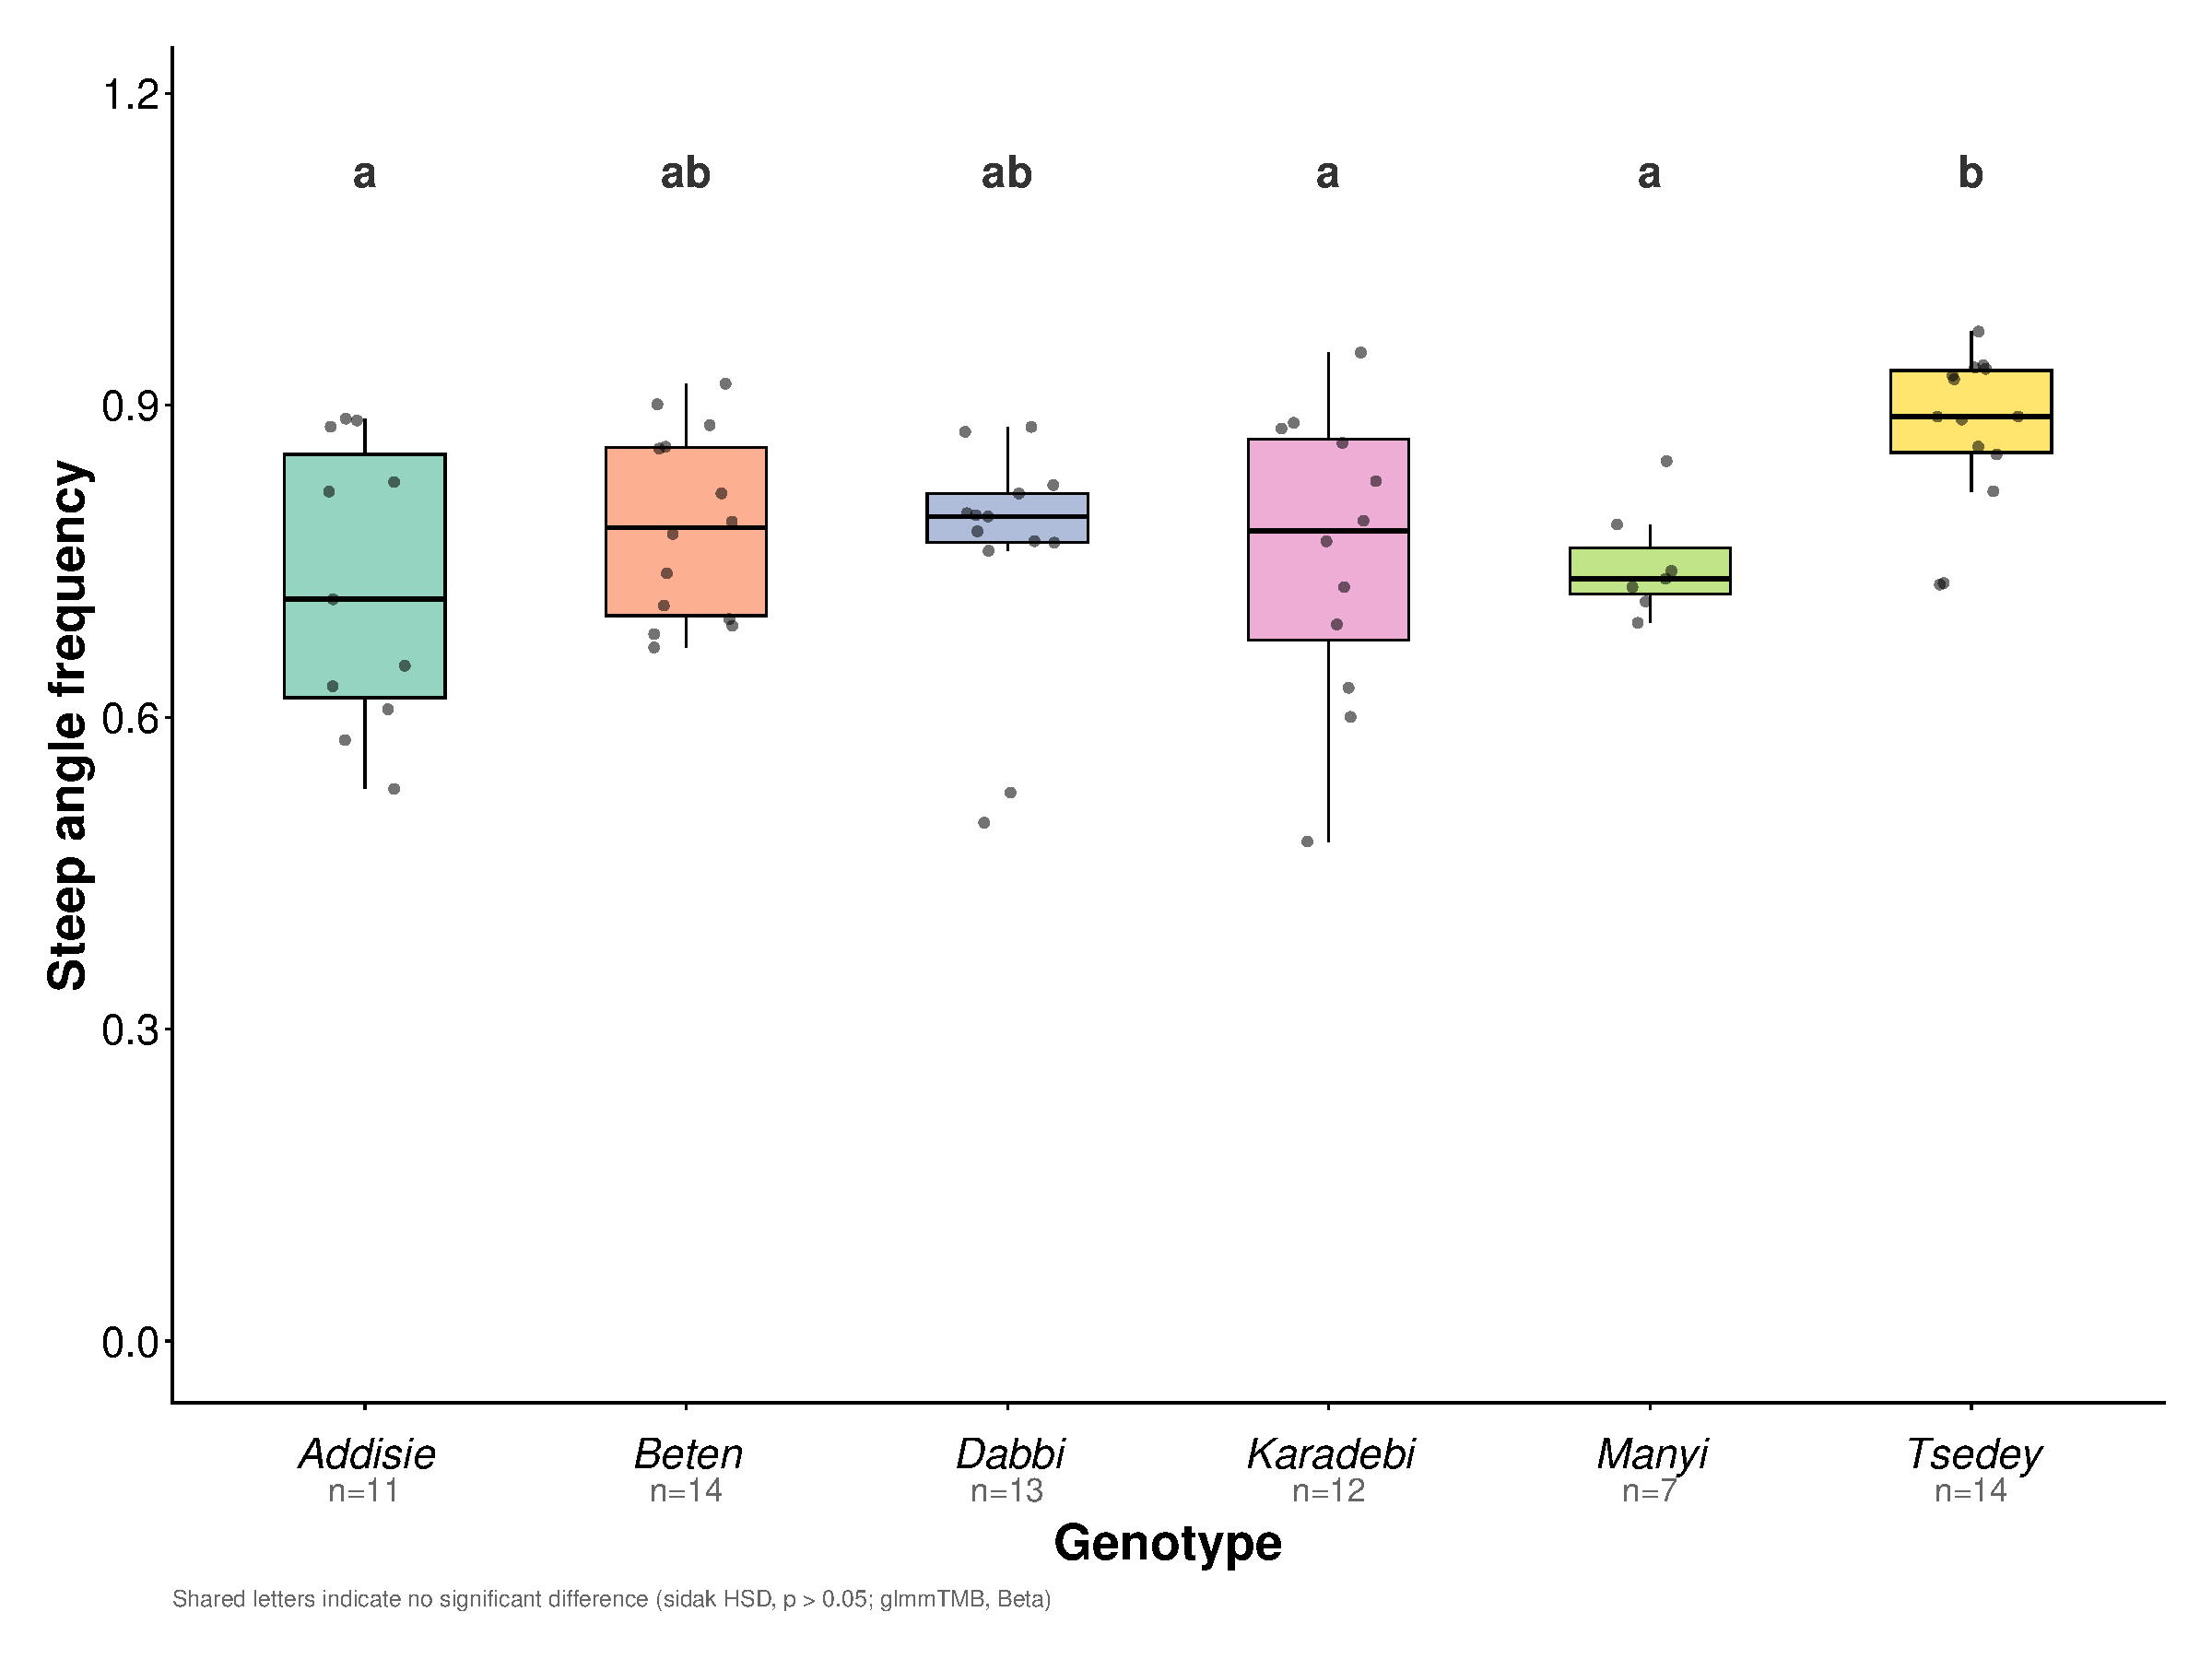
\includegraphics[keepaspectratio]{rsa_day1617_agar_files/figure-pdf/unnamed-chunk-9-11.pdf}}

\begin{Shaded}
\begin{Highlighting}[]
\CommentTok{\# difference here is where Dabbi groups {-} will go with full model for the figure as the model fit was better but good to see largely the same significant differences. }
\end{Highlighting}
\end{Shaded}

\subsubsection{Depth}\label{depth}

\begin{Shaded}
\begin{Highlighting}[]
\CommentTok{\# ============================================================}
\CommentTok{\#  Depth Analysis}
\CommentTok{\#  Positive continuous — start raw Gaussian, log if needed}
\CommentTok{\# ============================================================}

\CommentTok{\# ── 1. Inspect distribution ───────────────────────────────────}
\FunctionTok{summary}\NormalTok{(df}\SpecialCharTok{$}\NormalTok{Depth.mm)}
\end{Highlighting}
\end{Shaded}

\begin{verbatim}
   Min. 1st Qu.  Median    Mean 3rd Qu.    Max. 
  20.67   40.02   59.50   57.02   72.61   88.68 
\end{verbatim}

\begin{Shaded}
\begin{Highlighting}[]
\FunctionTok{hist}\NormalTok{(df}\SpecialCharTok{$}\NormalTok{Depth.mm, }\AttributeTok{breaks =} \DecValTok{15}\NormalTok{, }\AttributeTok{main =} \StringTok{"Depth distribution"}\NormalTok{)}
\end{Highlighting}
\end{Shaded}

\pandocbounded{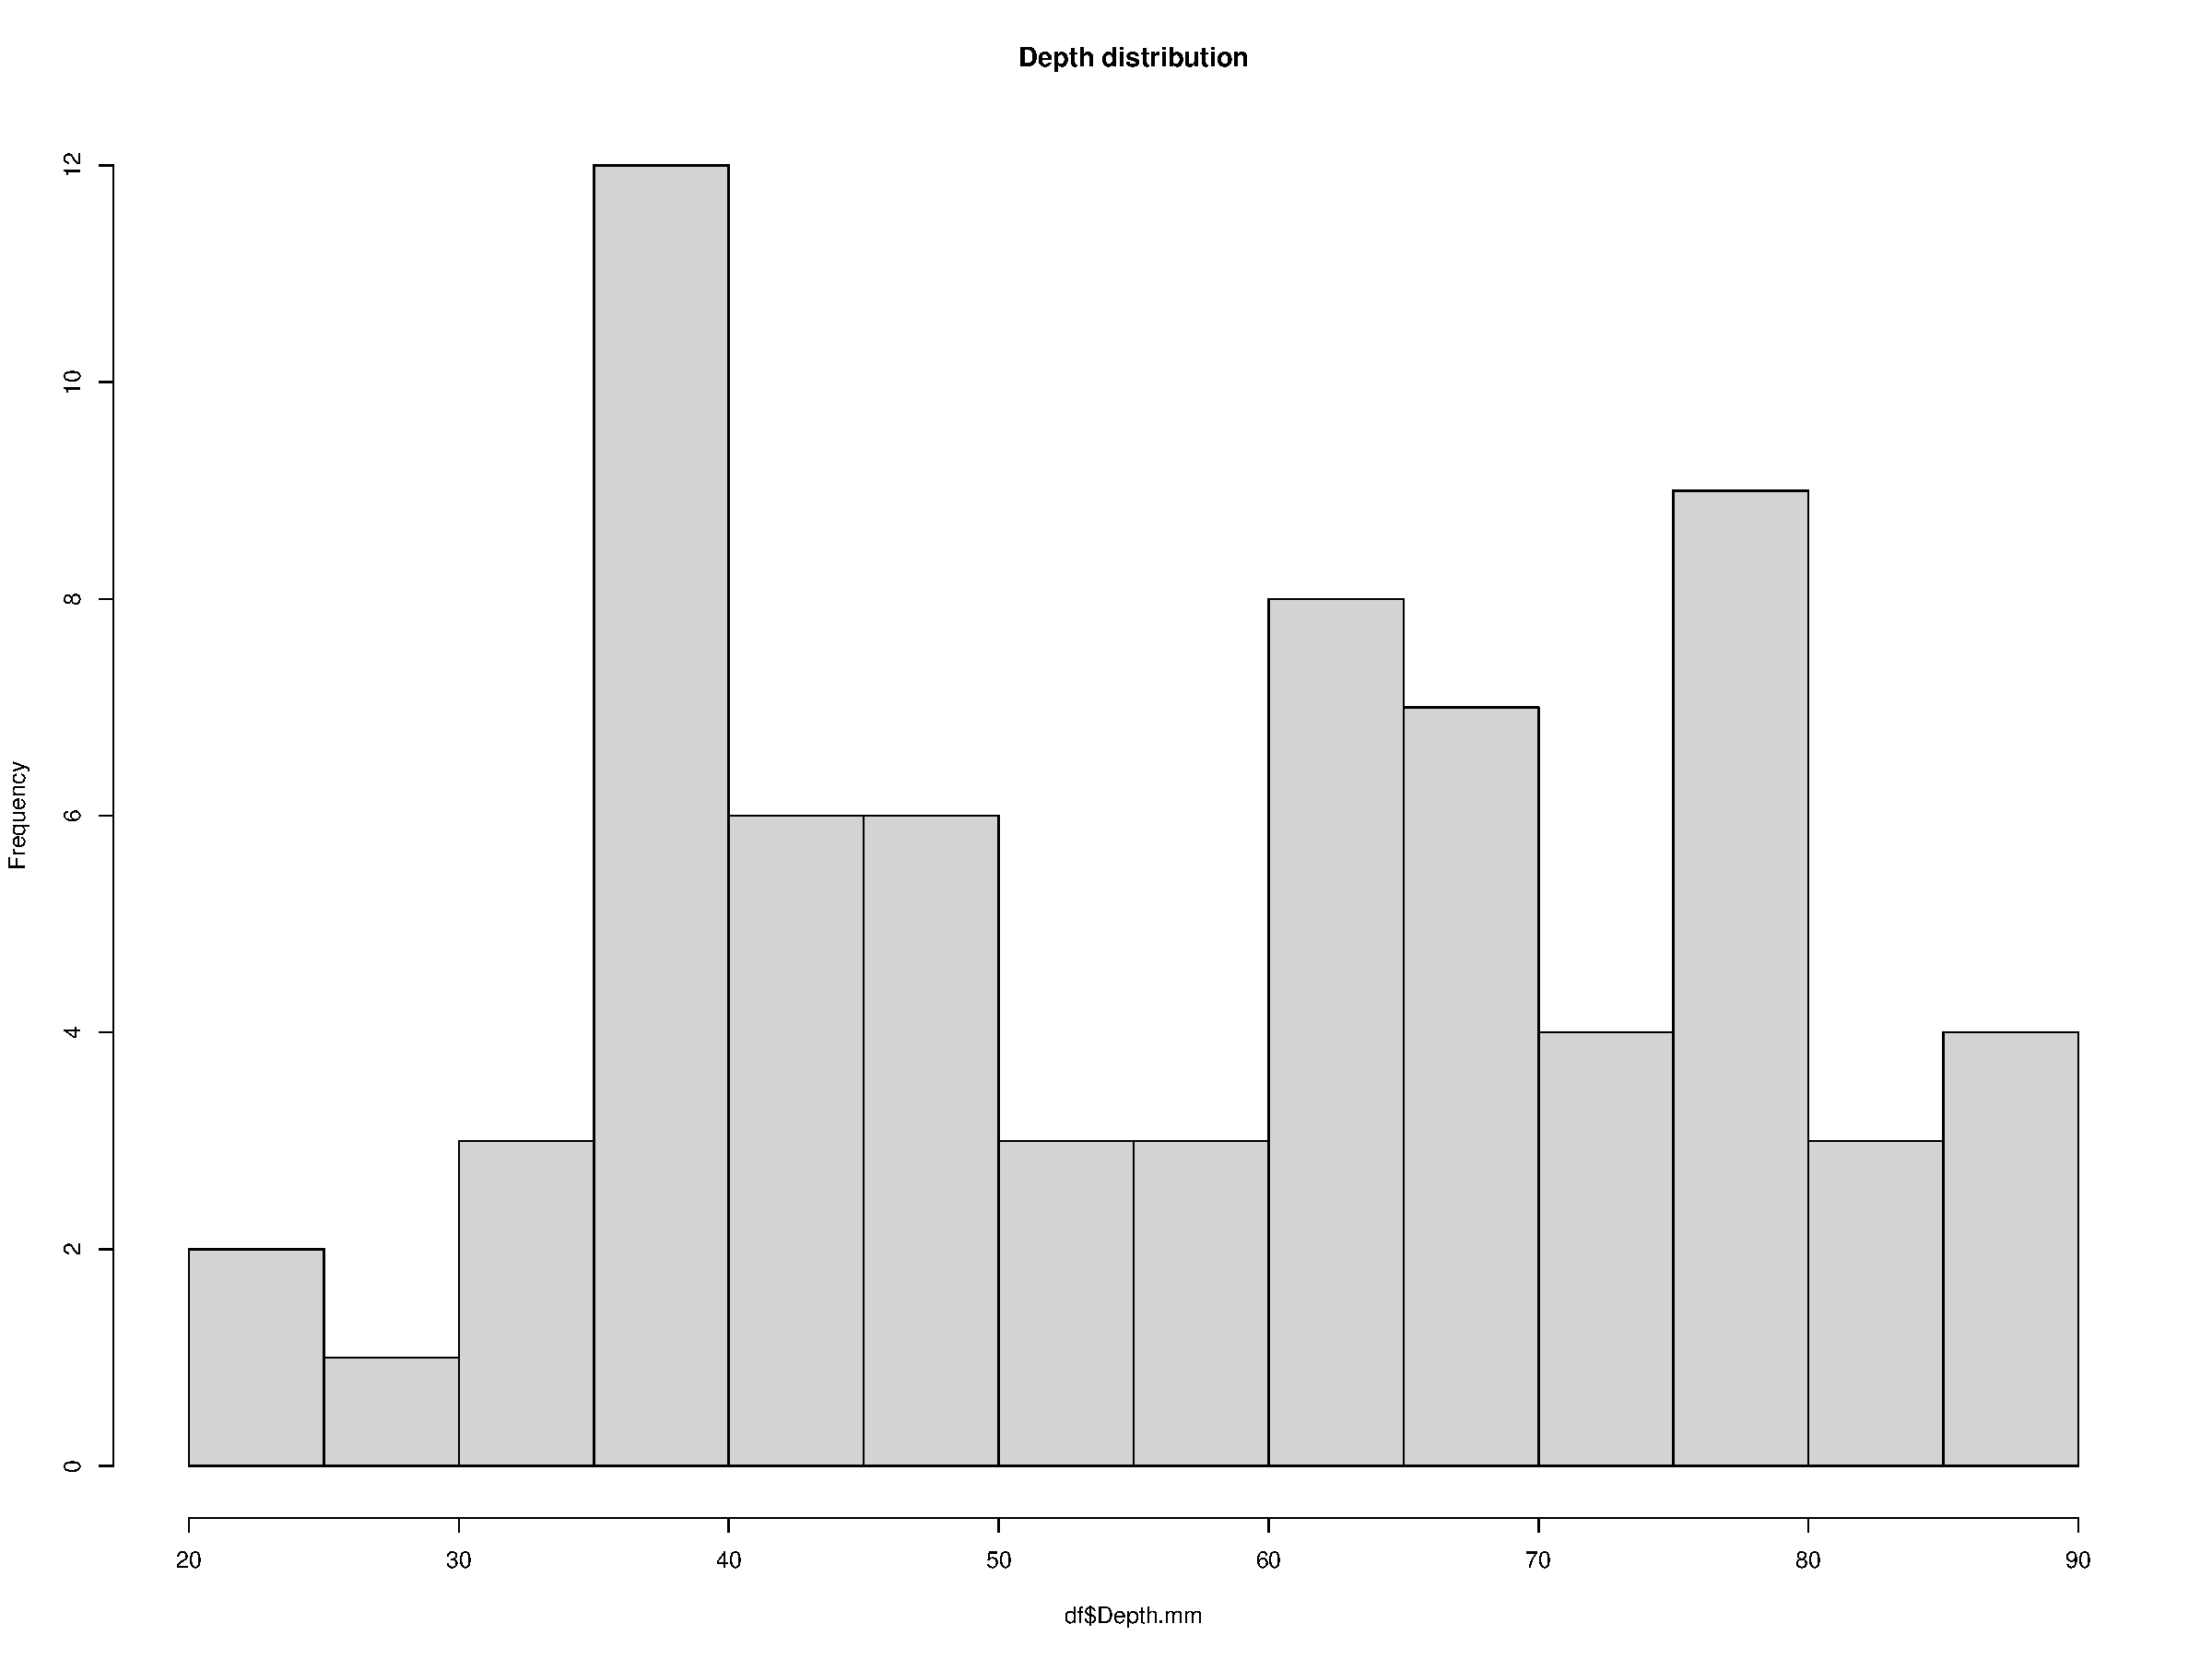
\includegraphics[keepaspectratio]{rsa_day1617_agar_files/figure-pdf/unnamed-chunk-10-1.pdf}}

\begin{Shaded}
\begin{Highlighting}[]
\CommentTok{\# ── 2. Fit full nested model ──────────────────────────────────}
\NormalTok{depth\_full }\OtherTok{\textless{}{-}} \FunctionTok{glmmTMB}\NormalTok{(}
\NormalTok{  Depth.mm }\SpecialCharTok{\textasciitilde{}}\NormalTok{ Genotype }\SpecialCharTok{+}\NormalTok{ (}\DecValTok{1} \SpecialCharTok{|}\NormalTok{ Batch}\SpecialCharTok{/}\NormalTok{Plate}\SpecialCharTok{/}\NormalTok{Seed),}
  \AttributeTok{data =}\NormalTok{ df, }\AttributeTok{family =} \FunctionTok{gaussian}\NormalTok{()}
\NormalTok{)}

\FunctionTok{VarCorr}\NormalTok{(depth\_full)}
\end{Highlighting}
\end{Shaded}

\begin{verbatim}

Conditional model:
 Groups           Name        Std.Dev.
 Seed:Plate:Batch (Intercept)  4.5680 
 Plate:Batch      (Intercept)  6.7937 
 Batch            (Intercept) 10.9865 
 Residual                     10.9642 
\end{verbatim}

\begin{Shaded}
\begin{Highlighting}[]
\FunctionTok{check\_singularity}\NormalTok{(depth\_full)}
\end{Highlighting}
\end{Shaded}

\begin{verbatim}
[1] FALSE
\end{verbatim}

\begin{Shaded}
\begin{Highlighting}[]
\FunctionTok{summary}\NormalTok{(depth\_full)}
\end{Highlighting}
\end{Shaded}

\begin{verbatim}
 Family: gaussian  ( identity )
Formula:          Depth.mm ~ Genotype + (1 | Batch/Plate/Seed)
Data: df

      AIC       BIC    logLik -2*log(L)  df.resid 
    591.5     614.1    -285.7     571.5        61 

Random effects:

Conditional model:
 Groups           Name        Variance Std.Dev.
 Seed:Plate:Batch (Intercept)  20.87    4.568  
 Plate:Batch      (Intercept)  46.15    6.794  
 Batch            (Intercept) 120.70   10.987  
 Residual                     120.21   10.964  
Number of obs: 71, groups:  Seed:Plate:Batch, 38; Plate:Batch, 18; Batch, 4

Dispersion estimate for gaussian family (sigma^2):  120 

Conditional model:
                 Estimate Std. Error z value Pr(>|z|)    
(Intercept)        60.387      6.956   8.682   <2e-16 ***
GenotypeBeten       1.800      4.703   0.383    0.702    
GenotypeDabbi      -5.113      5.585  -0.915    0.360    
GenotypeKaradebi   -3.306      5.431  -0.609    0.543    
GenotypeManyi      -5.751      6.339  -0.907    0.364    
GenotypeTsedey     -1.070      5.221  -0.205    0.838    
---
Signif. codes:  0 '***' 0.001 '**' 0.01 '*' 0.05 '.' 0.1 ' ' 1
\end{verbatim}

\begin{Shaded}
\begin{Highlighting}[]
\CommentTok{\# fit looks good so happy to continue with this but will do some assumption checks }

\CommentTok{\# ── 4. Assumption checks ─────}
\NormalTok{sim\_res }\OtherTok{\textless{}{-}} \FunctionTok{simulateResiduals}\NormalTok{(depth\_full, }\AttributeTok{n =} \DecValTok{1000}\NormalTok{)}
\FunctionTok{plot}\NormalTok{(sim\_res)}
\end{Highlighting}
\end{Shaded}

\pandocbounded{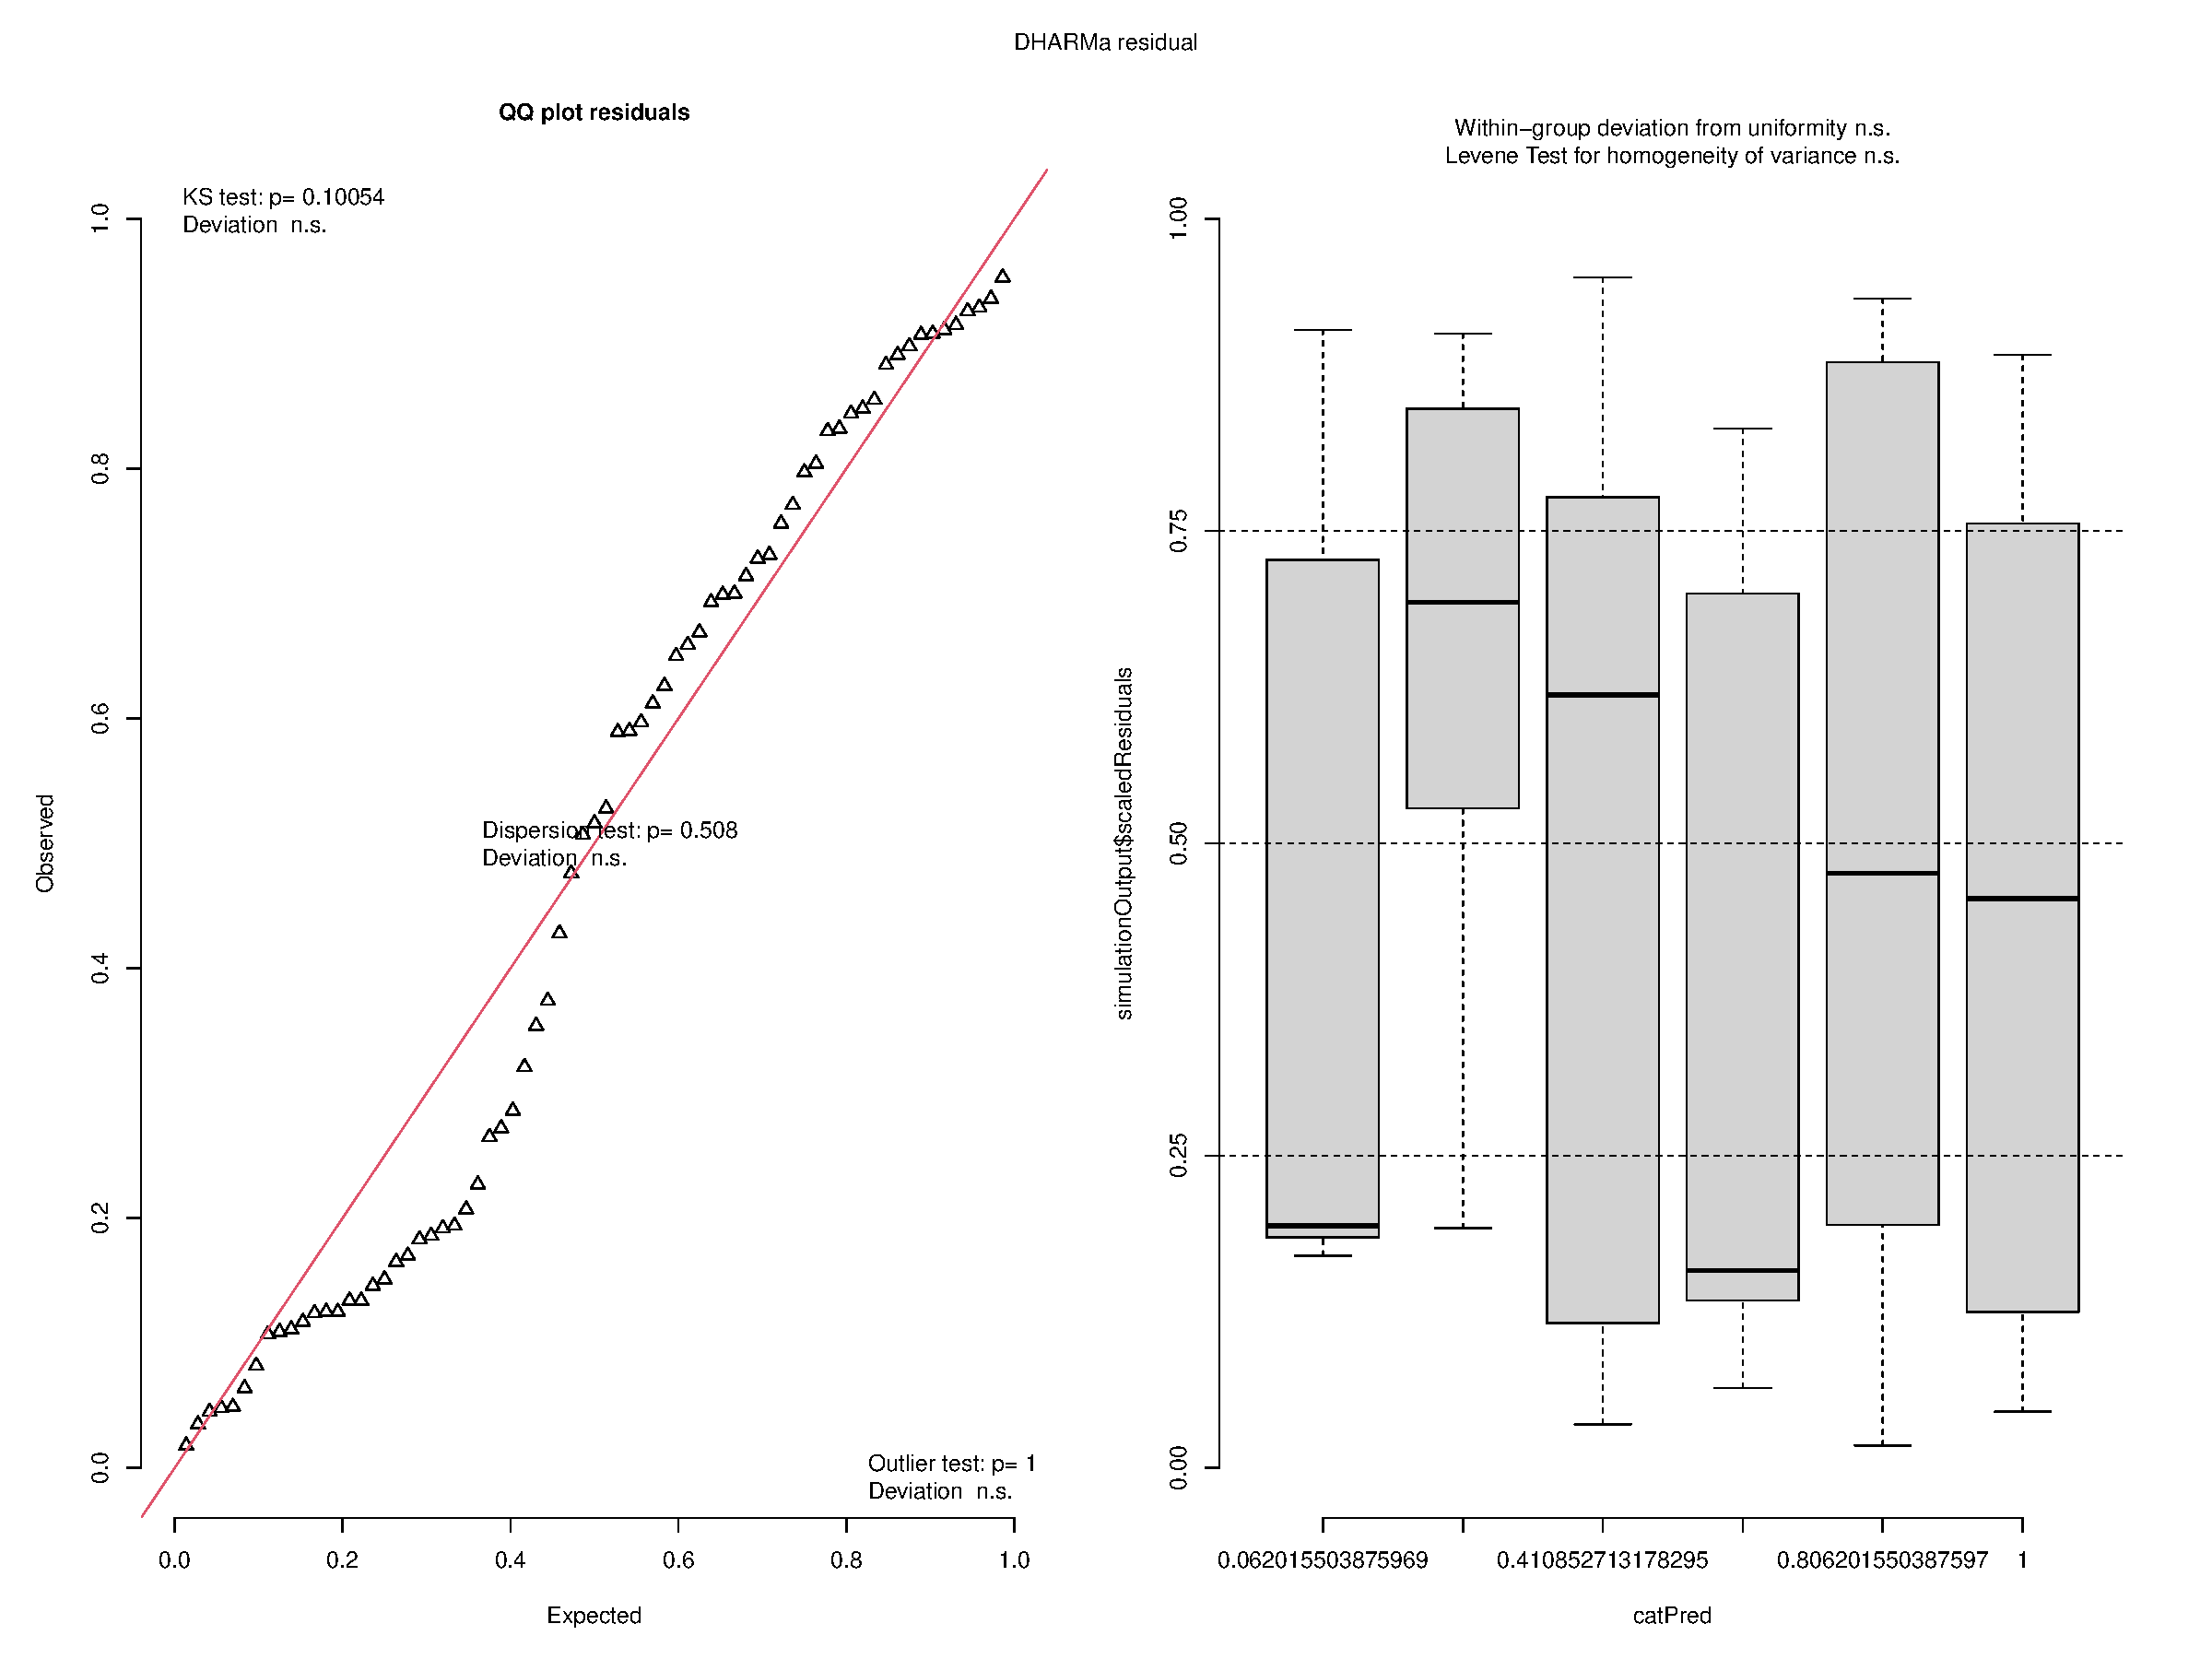
\includegraphics[keepaspectratio]{rsa_day1617_agar_files/figure-pdf/unnamed-chunk-10-2.pdf}}

\begin{Shaded}
\begin{Highlighting}[]
\FunctionTok{testUniformity}\NormalTok{(sim\_res)                     }\CommentTok{\# p \textgreater{} 0.05 = raw Gaussian fine}
\end{Highlighting}
\end{Shaded}

\pandocbounded{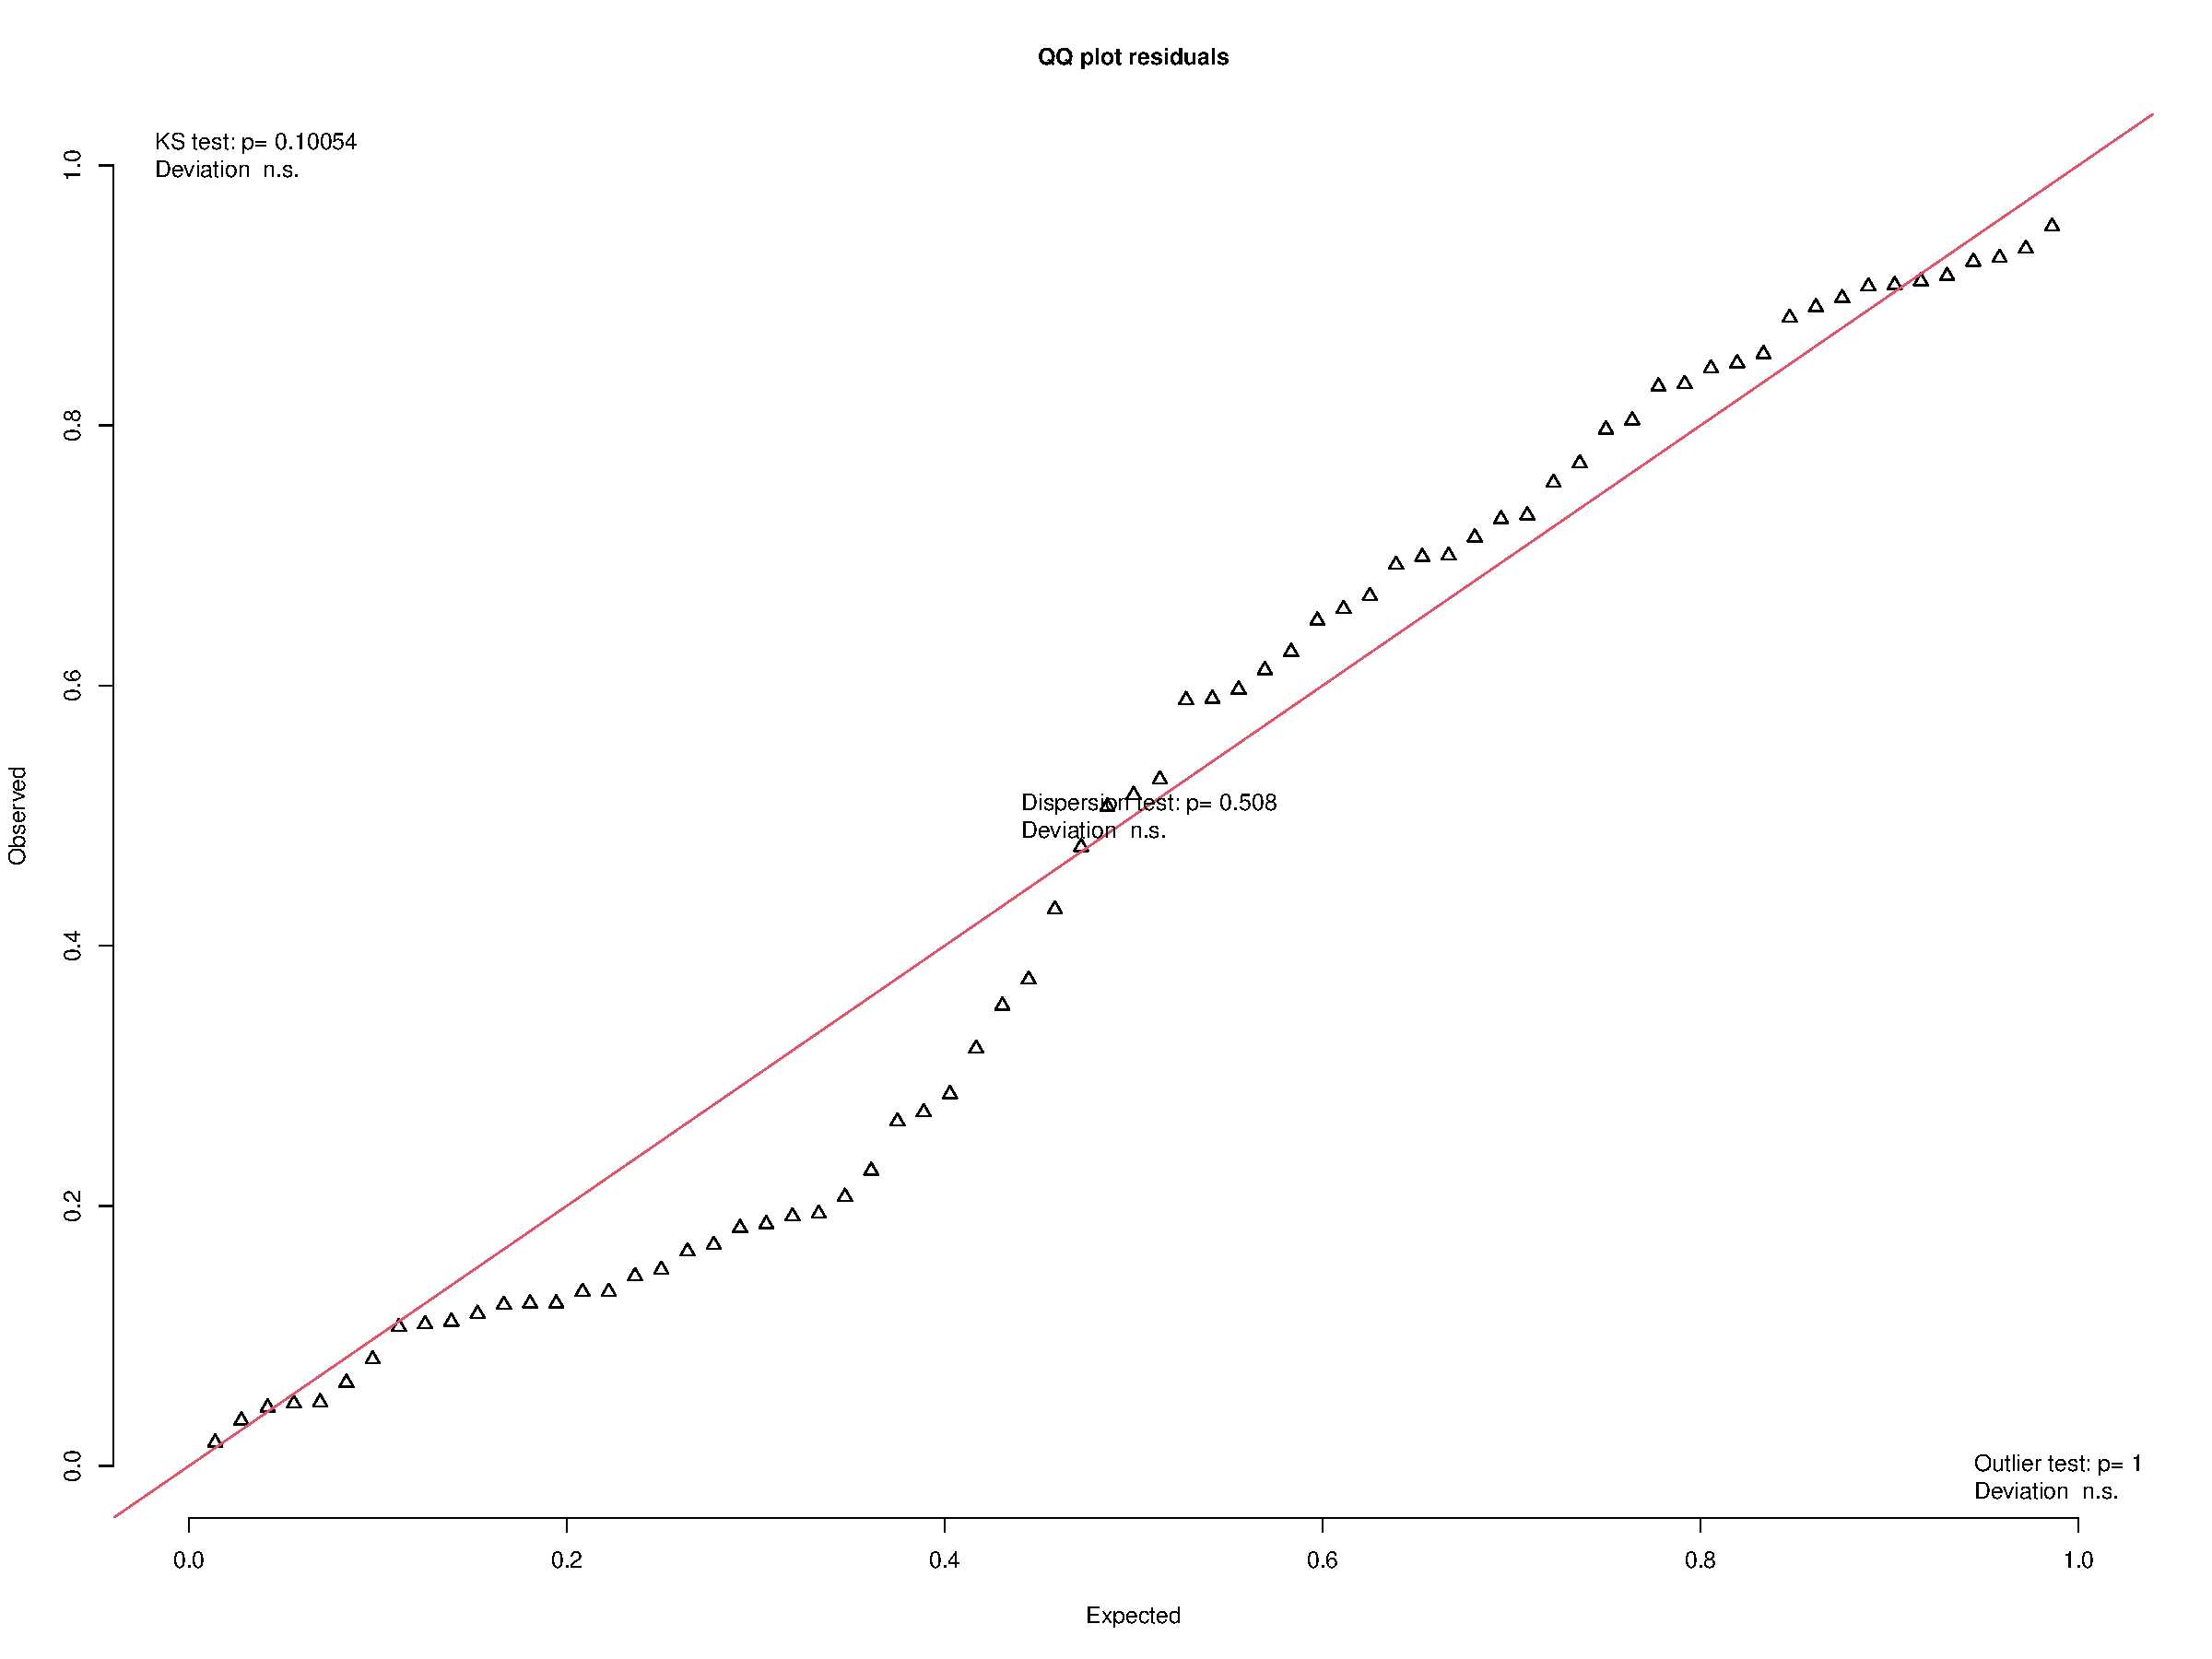
\includegraphics[keepaspectratio]{rsa_day1617_agar_files/figure-pdf/unnamed-chunk-10-3.pdf}}

\begin{verbatim}

    Asymptotic one-sample Kolmogorov-Smirnov test

data:  simulationOutput$scaledResiduals
D = 0.14511, p-value = 0.1005
alternative hypothesis: two-sided
\end{verbatim}

\begin{Shaded}
\begin{Highlighting}[]
\FunctionTok{testDispersion}\NormalTok{(sim\_res)                     }\CommentTok{\# ratio ≈ 1.0}
\end{Highlighting}
\end{Shaded}

\pandocbounded{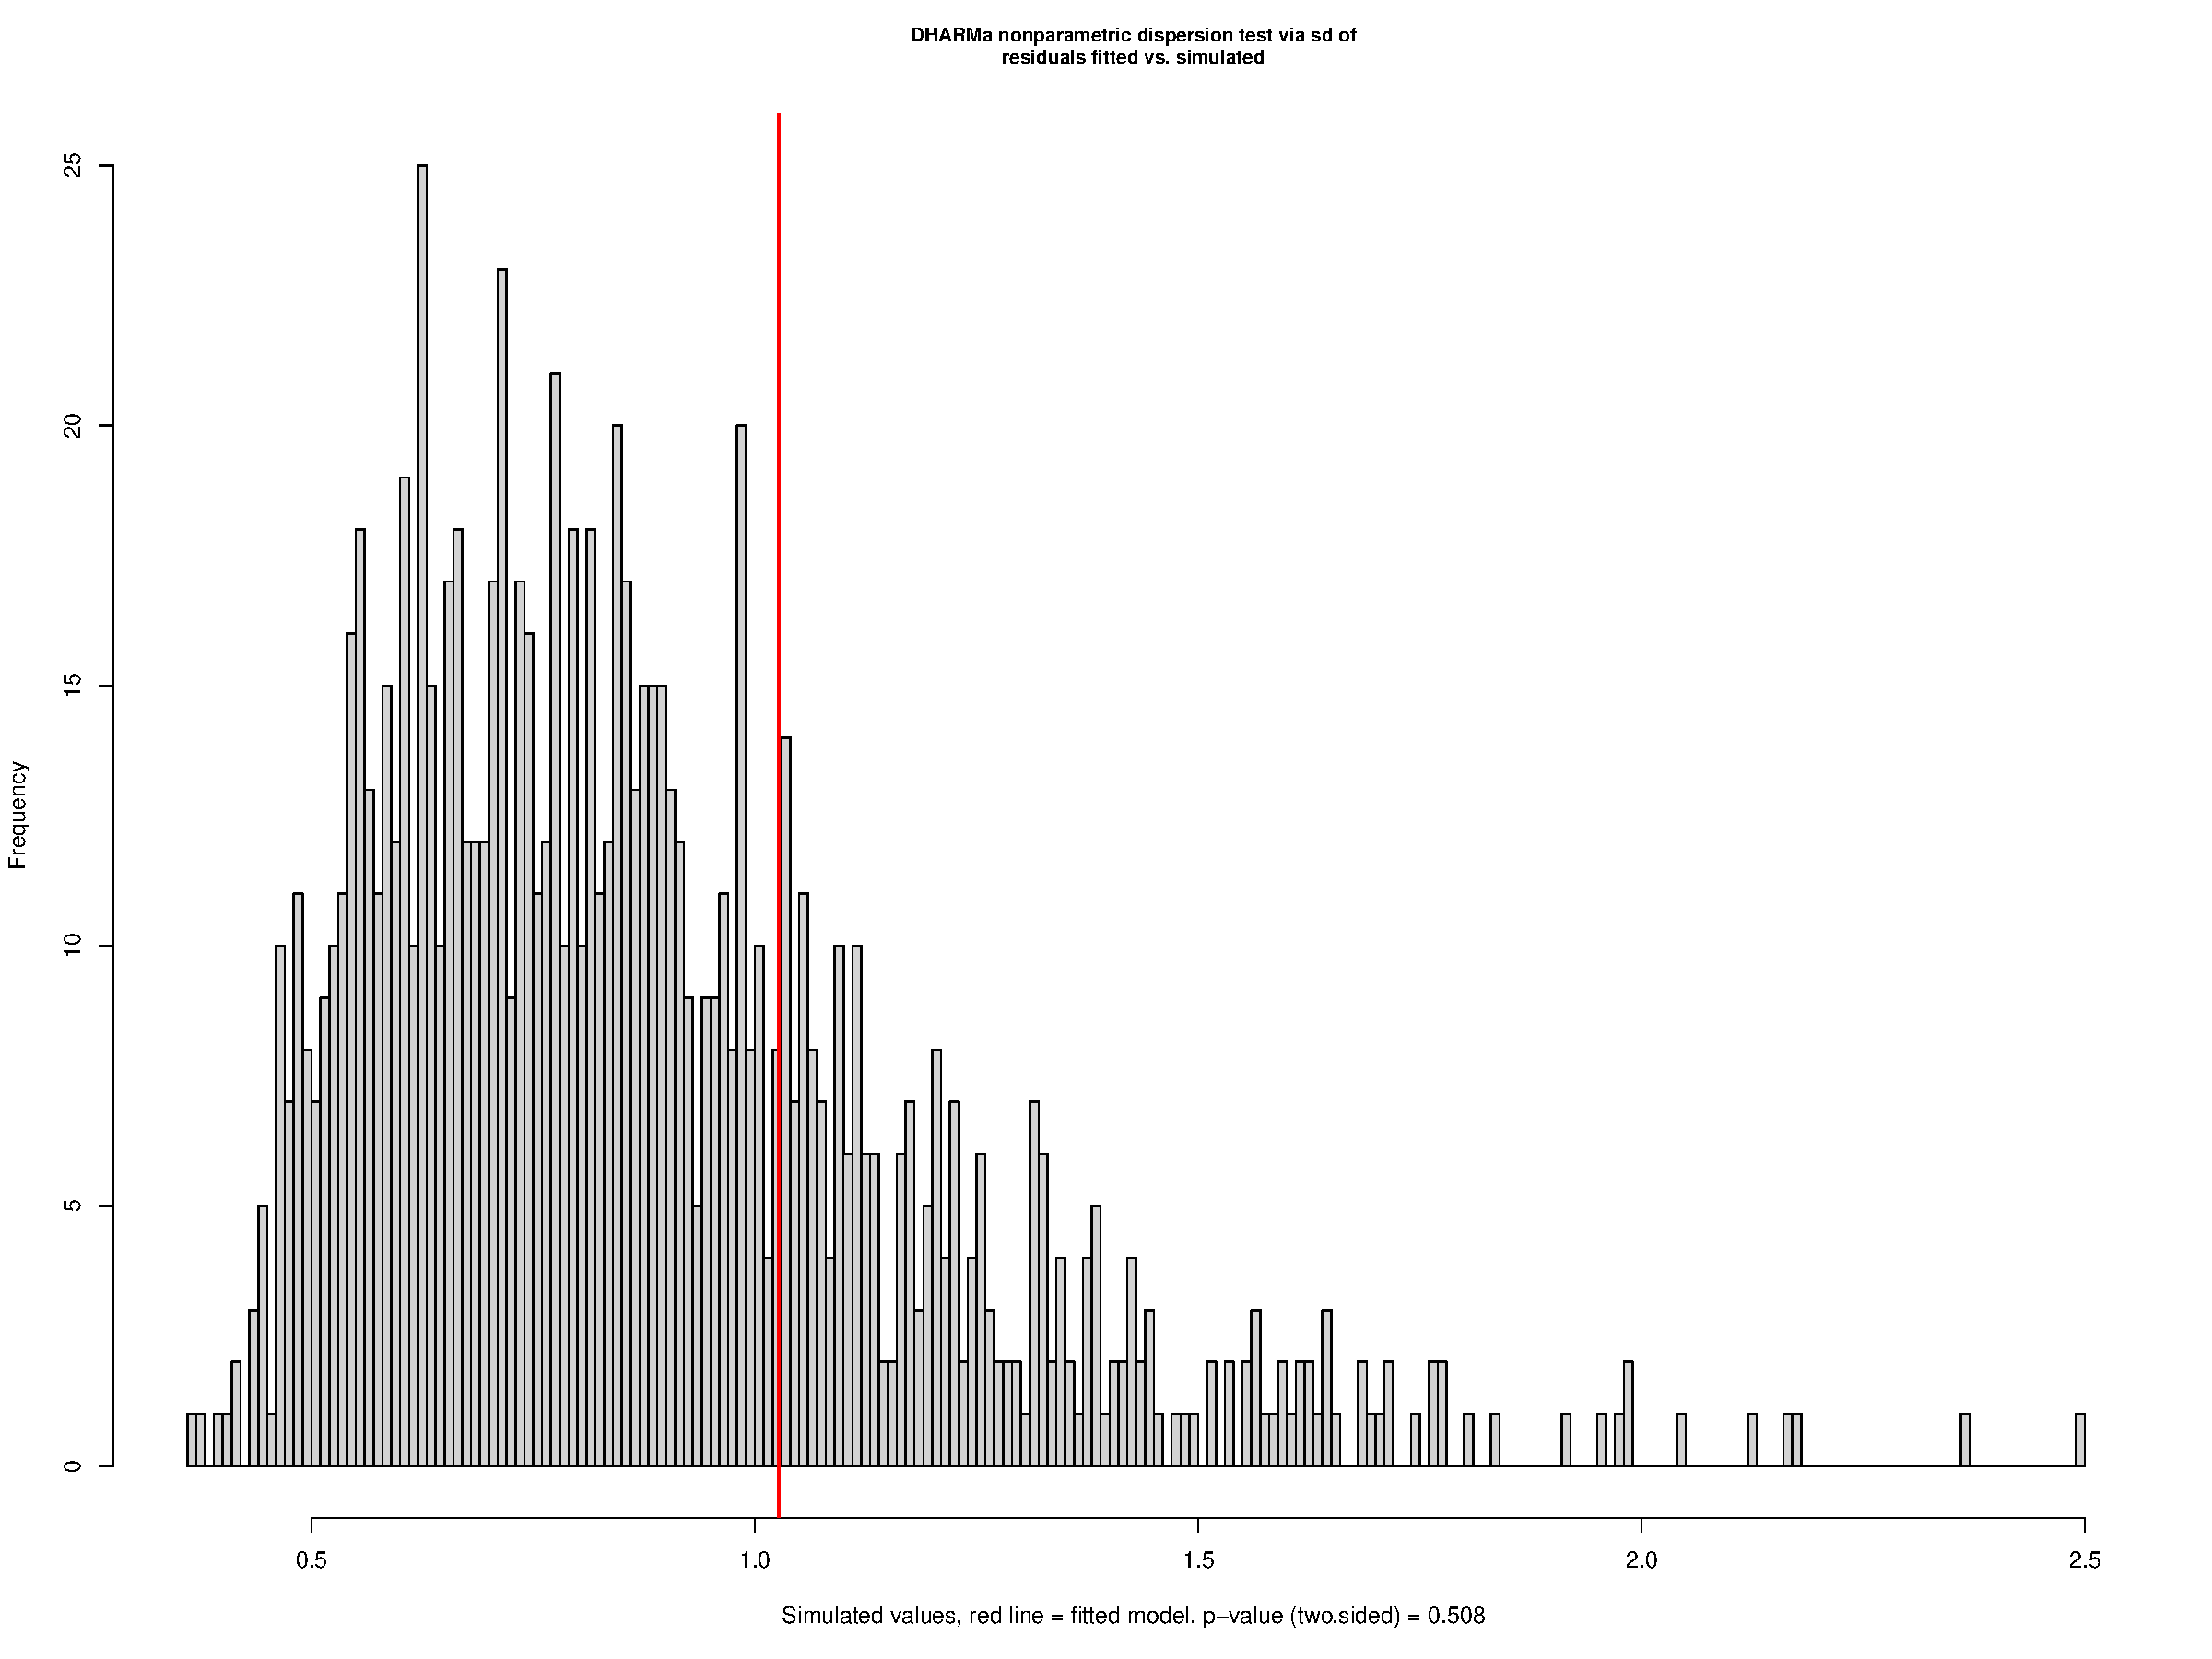
\includegraphics[keepaspectratio]{rsa_day1617_agar_files/figure-pdf/unnamed-chunk-10-4.pdf}}

\begin{verbatim}

    DHARMa nonparametric dispersion test via sd of residuals fitted vs.
    simulated

data:  simulationOutput
dispersion = 1.1728, p-value = 0.508
alternative hypothesis: two.sided
\end{verbatim}

\begin{Shaded}
\begin{Highlighting}[]
\FunctionTok{plotResiduals}\NormalTok{(sim\_res, }\AttributeTok{form =}\NormalTok{ df}\SpecialCharTok{$}\NormalTok{Genotype)}
\end{Highlighting}
\end{Shaded}

\pandocbounded{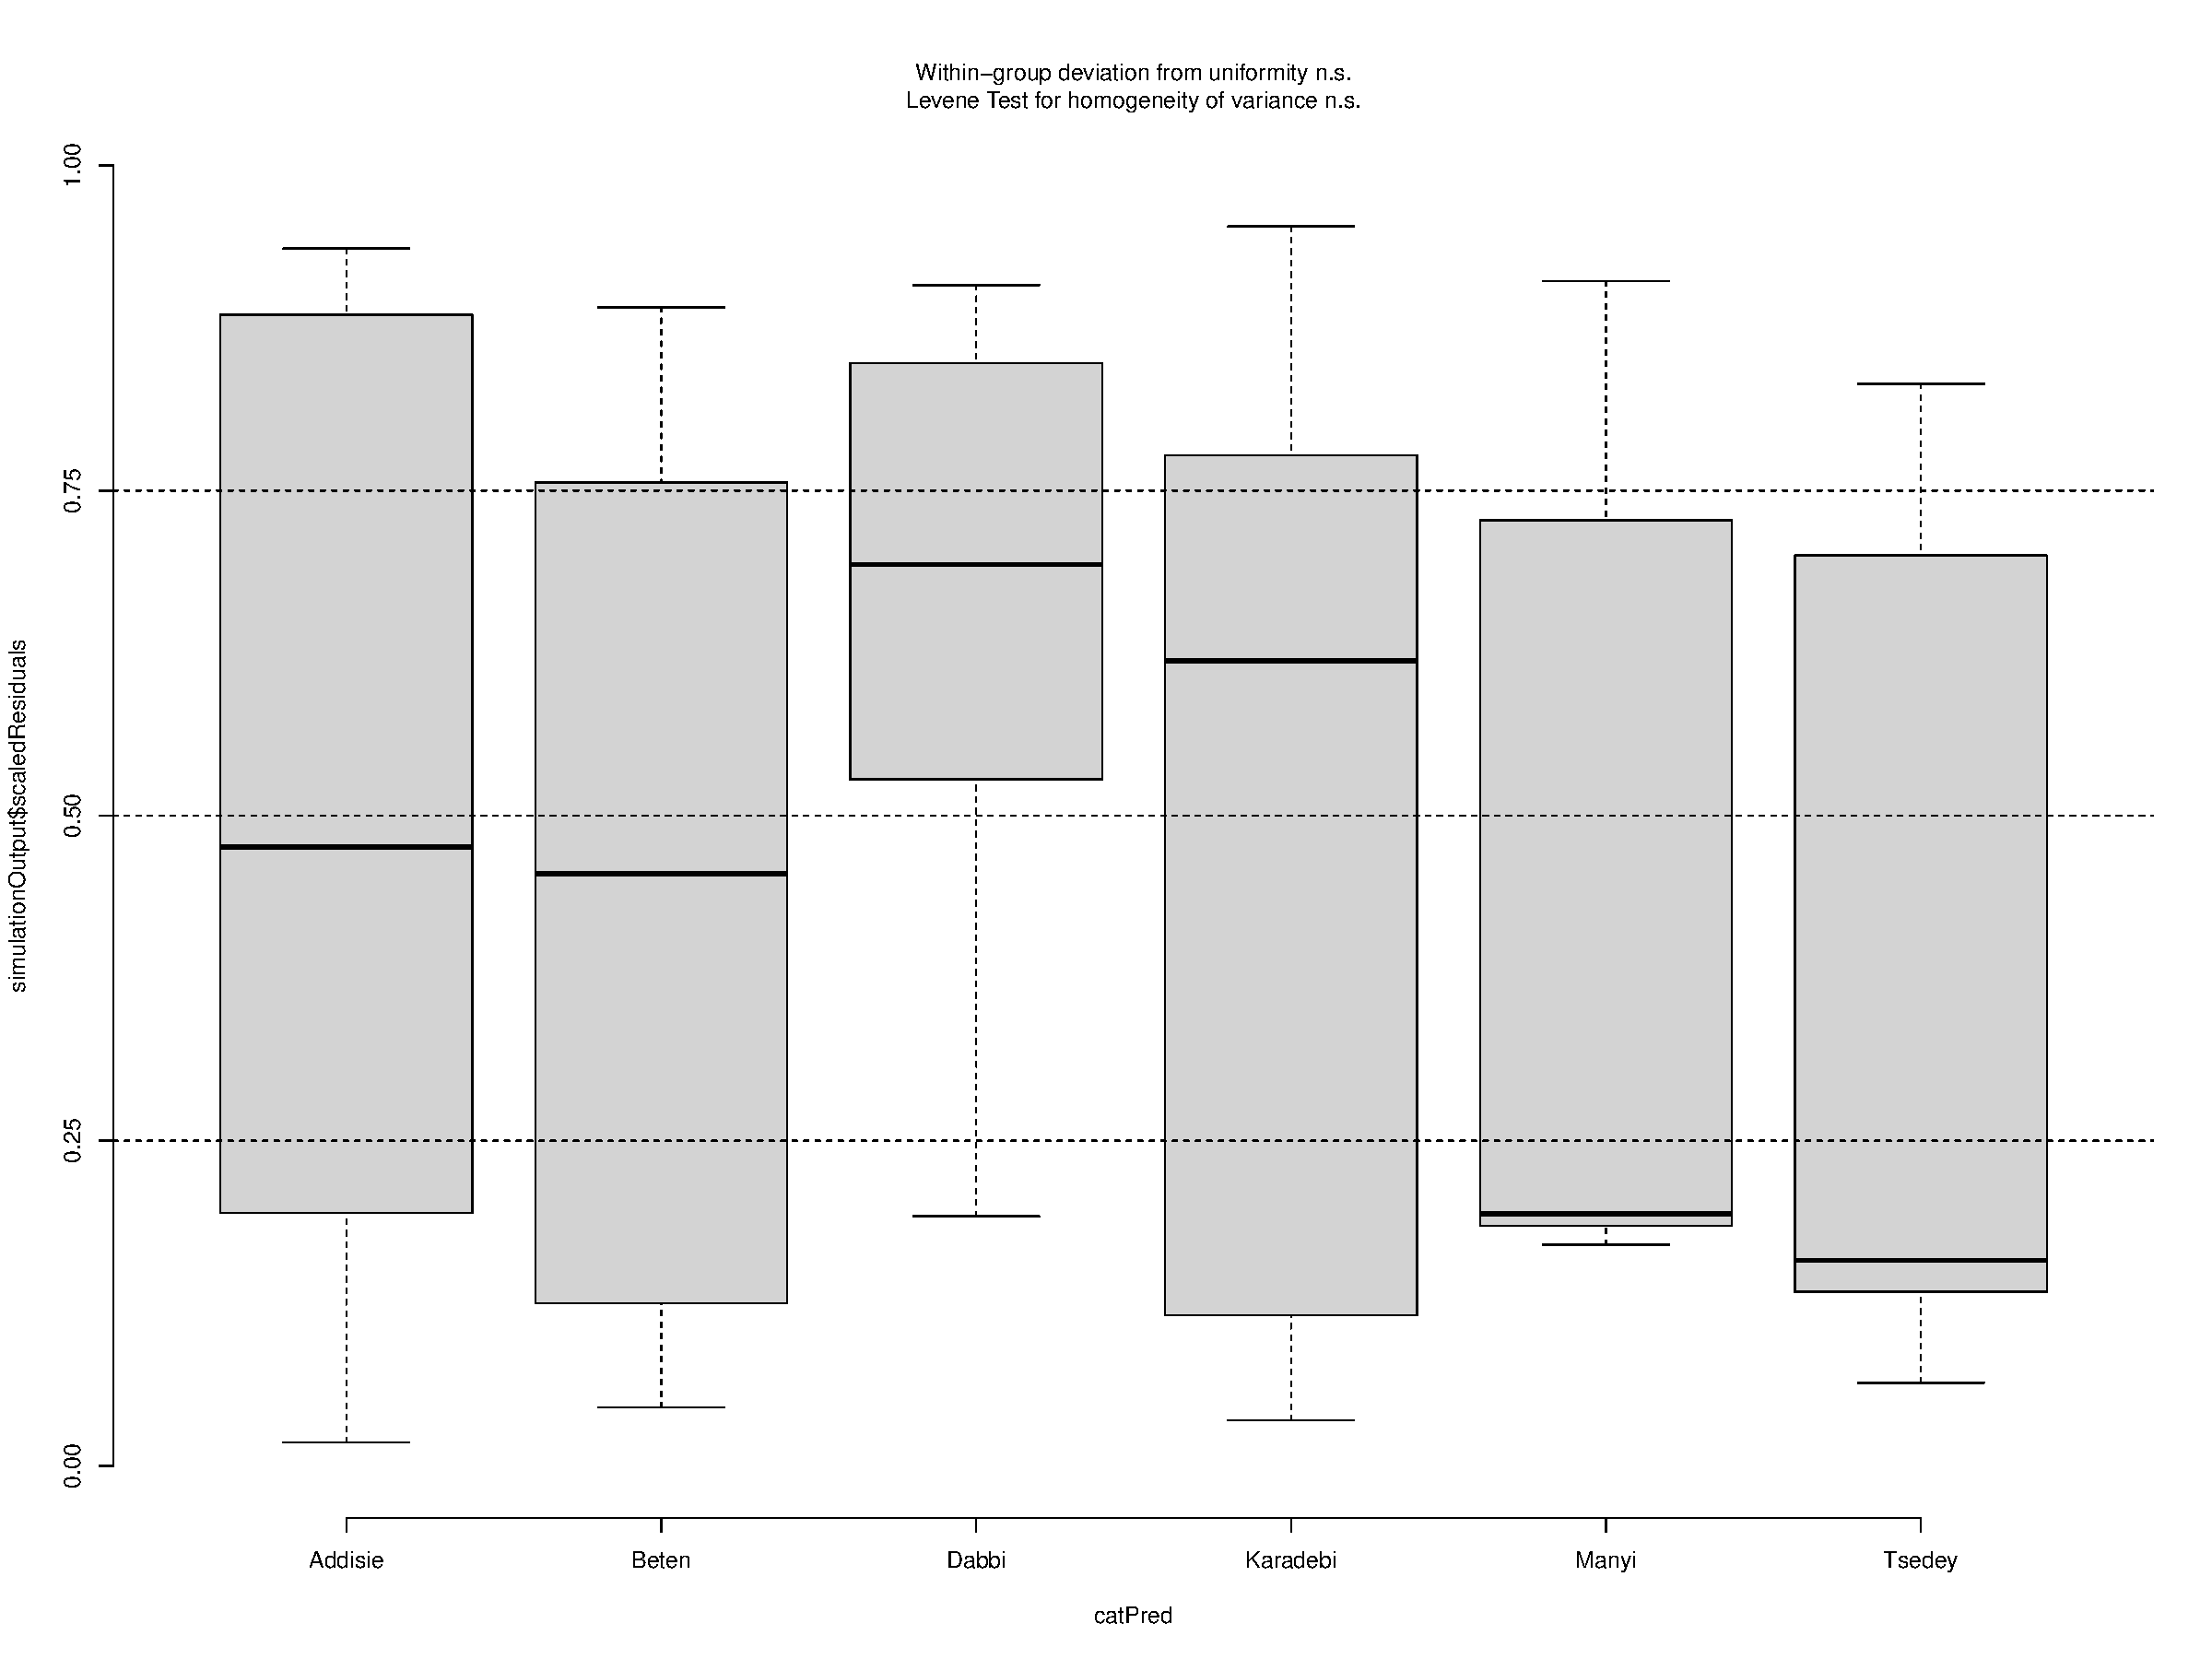
\includegraphics[keepaspectratio]{rsa_day1617_agar_files/figure-pdf/unnamed-chunk-10-5.pdf}}

\begin{Shaded}
\begin{Highlighting}[]
\CommentTok{\# ── 5. Test overall Genotype effect ──────────────────────────}
\NormalTok{car}\SpecialCharTok{::}\FunctionTok{Anova}\NormalTok{(depth\_full, }\AttributeTok{type =} \StringTok{"III"}\NormalTok{)}
\end{Highlighting}
\end{Shaded}

\begin{verbatim}
Analysis of Deviance Table (Type III Wald chisquare tests)

Response: Depth.mm
              Chisq Df Pr(>Chisq)    
(Intercept) 75.3702  1     <2e-16 ***
Genotype     2.4006  5     0.7914    
---
Signif. codes:  0 '***' 0.001 '**' 0.01 '*' 0.05 '.' 0.1 ' ' 1
\end{verbatim}

\begin{Shaded}
\begin{Highlighting}[]
\CommentTok{\# ── 6. Pairwise comparisons + CLD ────────────────────────────}
\NormalTok{emm }\OtherTok{\textless{}{-}} \FunctionTok{emmeans}\NormalTok{(depth\_full, }\SpecialCharTok{\textasciitilde{}}\NormalTok{ Genotype)}
\FunctionTok{pairs}\NormalTok{(emm, }\AttributeTok{adjust =} \StringTok{"sidak"}\NormalTok{)}
\end{Highlighting}
\end{Shaded}

\begin{verbatim}
 contrast           estimate   SE  df z.ratio p.value
 Addisie - Beten      -1.800 4.70 Inf  -0.383  1.0000
 Addisie - Dabbi       5.113 5.59 Inf   0.915  0.9988
 Addisie - Karadebi    3.306 5.43 Inf   0.609  1.0000
 Addisie - Manyi       5.751 6.34 Inf   0.907  0.9989
 Addisie - Tsedey      1.070 5.22 Inf   0.205  1.0000
 Beten - Dabbi         6.913 5.27 Inf   1.312  0.9572
 Beten - Karadebi      5.106 5.16 Inf   0.989  0.9971
 Beten - Manyi         7.551 5.89 Inf   1.282  0.9646
 Beten - Tsedey        2.870 4.85 Inf   0.592  1.0000
 Dabbi - Karadebi     -1.807 4.96 Inf  -0.364  1.0000
 Dabbi - Manyi         0.638 5.81 Inf   0.110  1.0000
 Dabbi - Tsedey       -4.043 5.63 Inf  -0.718  0.9999
 Karadebi - Manyi      2.445 5.79 Inf   0.422  1.0000
 Karadebi - Tsedey    -2.236 5.49 Inf  -0.407  1.0000
 Manyi - Tsedey       -4.681 5.82 Inf  -0.804  0.9997

P value adjustment: sidak method for 15 tests 
\end{verbatim}

\begin{Shaded}
\begin{Highlighting}[]
\NormalTok{cld\_df }\OtherTok{\textless{}{-}} \FunctionTok{as.data.frame}\NormalTok{(}\FunctionTok{cld}\NormalTok{(emm, }\AttributeTok{adjust =} \StringTok{"sidak"}\NormalTok{,}
                             \AttributeTok{Letters =}\NormalTok{ letters, }\AttributeTok{alpha =} \FloatTok{0.05}\NormalTok{)) }\SpecialCharTok{\%\textgreater{}\%}
  \FunctionTok{mutate}\NormalTok{(}\AttributeTok{.group =} \FunctionTok{trimws}\NormalTok{(.group))}

\NormalTok{n\_df }\OtherTok{\textless{}{-}}\NormalTok{ df }\SpecialCharTok{\%\textgreater{}\%}
  \FunctionTok{count}\NormalTok{(Genotype) }\SpecialCharTok{\%\textgreater{}\%}
  \FunctionTok{mutate}\NormalTok{(}\AttributeTok{label =} \FunctionTok{paste0}\NormalTok{(}\StringTok{"n="}\NormalTok{, n))}


\CommentTok{\# ── 7. Plot 1 — Boxplot ───────────────────────────────────────}

\NormalTok{y\_ceil }\OtherTok{\textless{}{-}} \FunctionTok{max}\NormalTok{(df}\SpecialCharTok{$}\NormalTok{Depth.mm) }\SpecialCharTok{*} \FloatTok{1.22}
\NormalTok{y\_label }\OtherTok{\textless{}{-}}\NormalTok{ y\_ceil }\SpecialCharTok{*} \FloatTok{0.95}

\NormalTok{p1 }\OtherTok{\textless{}{-}} \FunctionTok{ggplot}\NormalTok{(df, }\FunctionTok{aes}\NormalTok{(}\AttributeTok{x =}\NormalTok{ Genotype, }\AttributeTok{y =}\NormalTok{ Depth.mm, }\AttributeTok{fill =}\NormalTok{ Genotype)) }\SpecialCharTok{+}

  \FunctionTok{geom\_boxplot}\NormalTok{(}
    \AttributeTok{alpha         =} \FloatTok{0.7}\NormalTok{,}
    \AttributeTok{outlier.shape =} \ConstantTok{NA}\NormalTok{,}
    \AttributeTok{width         =} \FloatTok{0.5}\NormalTok{,}
    \AttributeTok{colour        =} \StringTok{"black"}\NormalTok{,}
    \AttributeTok{linewidth     =} \FloatTok{0.5}
\NormalTok{  ) }\SpecialCharTok{+}

  \FunctionTok{geom\_jitter}\NormalTok{(}
    \AttributeTok{width  =} \FloatTok{0.15}\NormalTok{,}
    \AttributeTok{size   =} \FloatTok{1.8}\NormalTok{,}
    \AttributeTok{alpha  =} \FloatTok{0.55}\NormalTok{,}
    \AttributeTok{colour =} \StringTok{"black"}
\NormalTok{  ) }\SpecialCharTok{+}

  \FunctionTok{geom\_text}\NormalTok{(}
    \AttributeTok{data        =}\NormalTok{ cld\_df,}
    \FunctionTok{aes}\NormalTok{(}\AttributeTok{x =}\NormalTok{ Genotype, }\AttributeTok{label =}\NormalTok{ .group),}
    \AttributeTok{y           =}\NormalTok{ y\_label,}
    \AttributeTok{inherit.aes =} \ConstantTok{FALSE}\NormalTok{,}
    \AttributeTok{size        =} \DecValTok{5}\NormalTok{,}
    \AttributeTok{fontface    =} \StringTok{"bold"}\NormalTok{,}
    \AttributeTok{colour      =} \StringTok{"grey20"}
\NormalTok{  ) }\SpecialCharTok{+}

  \FunctionTok{geom\_text}\NormalTok{(}
    \AttributeTok{data        =}\NormalTok{ n\_df,}
    \FunctionTok{aes}\NormalTok{(}\AttributeTok{x =}\NormalTok{ Genotype, }\AttributeTok{label =}\NormalTok{ label),}
    \AttributeTok{y           =} \SpecialCharTok{{-}}\ConstantTok{Inf}\NormalTok{,}
    \AttributeTok{vjust       =} \FloatTok{4.2}\NormalTok{,}
    \AttributeTok{inherit.aes =} \ConstantTok{FALSE}\NormalTok{,}
    \AttributeTok{size        =} \FloatTok{3.5}\NormalTok{,}
    \AttributeTok{colour      =} \StringTok{"grey40"}
\NormalTok{  ) }\SpecialCharTok{+}

  \FunctionTok{scale\_fill\_brewer}\NormalTok{(}\AttributeTok{palette =} \StringTok{"Set2"}\NormalTok{) }\SpecialCharTok{+}

  \FunctionTok{labs}\NormalTok{(}
    \AttributeTok{x       =} \StringTok{"Genotype"}\NormalTok{,}
    \AttributeTok{y       =} \StringTok{"Depth (mm)"}\NormalTok{,}
    \AttributeTok{caption =} \StringTok{"Shared letters indicate no significant difference (sidak HSD, p \textgreater{} 0.05; glmmTMB, Gaussian)"}
\NormalTok{  ) }\SpecialCharTok{+}

  \FunctionTok{theme\_classic}\NormalTok{(}\AttributeTok{base\_size =} \DecValTok{14}\NormalTok{) }\SpecialCharTok{+}
  \FunctionTok{theme}\NormalTok{(}
    \AttributeTok{legend.position =} \StringTok{"none"}\NormalTok{,}
    \AttributeTok{axis.line       =} \FunctionTok{element\_line}\NormalTok{(}\AttributeTok{colour =} \StringTok{"black"}\NormalTok{, }\AttributeTok{linewidth =} \FloatTok{0.6}\NormalTok{),}
    \AttributeTok{axis.ticks      =} \FunctionTok{element\_line}\NormalTok{(}\AttributeTok{colour =} \StringTok{"black"}\NormalTok{, }\AttributeTok{linewidth =} \FloatTok{0.5}\NormalTok{),}
    \AttributeTok{axis.title      =} \FunctionTok{element\_text}\NormalTok{(}\AttributeTok{size =} \DecValTok{14}\NormalTok{, }\AttributeTok{face =} \StringTok{"bold"}\NormalTok{),}
    \AttributeTok{axis.text       =} \FunctionTok{element\_text}\NormalTok{(}\AttributeTok{size =} \DecValTok{14}\NormalTok{, }\AttributeTok{colour =} \StringTok{"black"}\NormalTok{),}
    \AttributeTok{axis.text.x     =} \FunctionTok{element\_text}\NormalTok{(}\AttributeTok{face =} \StringTok{"italic"}\NormalTok{, }\AttributeTok{margin =} \FunctionTok{margin}\NormalTok{(}\AttributeTok{t =} \DecValTok{3}\NormalTok{)),}
    \AttributeTok{plot.caption    =} \FunctionTok{element\_text}\NormalTok{(}\AttributeTok{size =} \DecValTok{9}\NormalTok{, }\AttributeTok{colour =} \StringTok{"grey40"}\NormalTok{, }\AttributeTok{hjust =} \DecValTok{0}\NormalTok{),}
    \AttributeTok{plot.margin     =} \FunctionTok{margin}\NormalTok{(}\AttributeTok{t =} \DecValTok{10}\NormalTok{, }\AttributeTok{r =} \DecValTok{15}\NormalTok{, }\AttributeTok{b =} \DecValTok{30}\NormalTok{, }\AttributeTok{l =} \DecValTok{10}\NormalTok{)}
\NormalTok{  )}

\NormalTok{p1 }\SpecialCharTok{+} \FunctionTok{coord\_cartesian}\NormalTok{(}
  \AttributeTok{ylim =} \FunctionTok{c}\NormalTok{(}\DecValTok{0}\NormalTok{, }\FunctionTok{max}\NormalTok{(df}\SpecialCharTok{$}\NormalTok{Depth.mm) }\SpecialCharTok{*} \FloatTok{1.22}\NormalTok{),}
  \AttributeTok{clip =} \StringTok{"off"}
\NormalTok{)}
\end{Highlighting}
\end{Shaded}

\pandocbounded{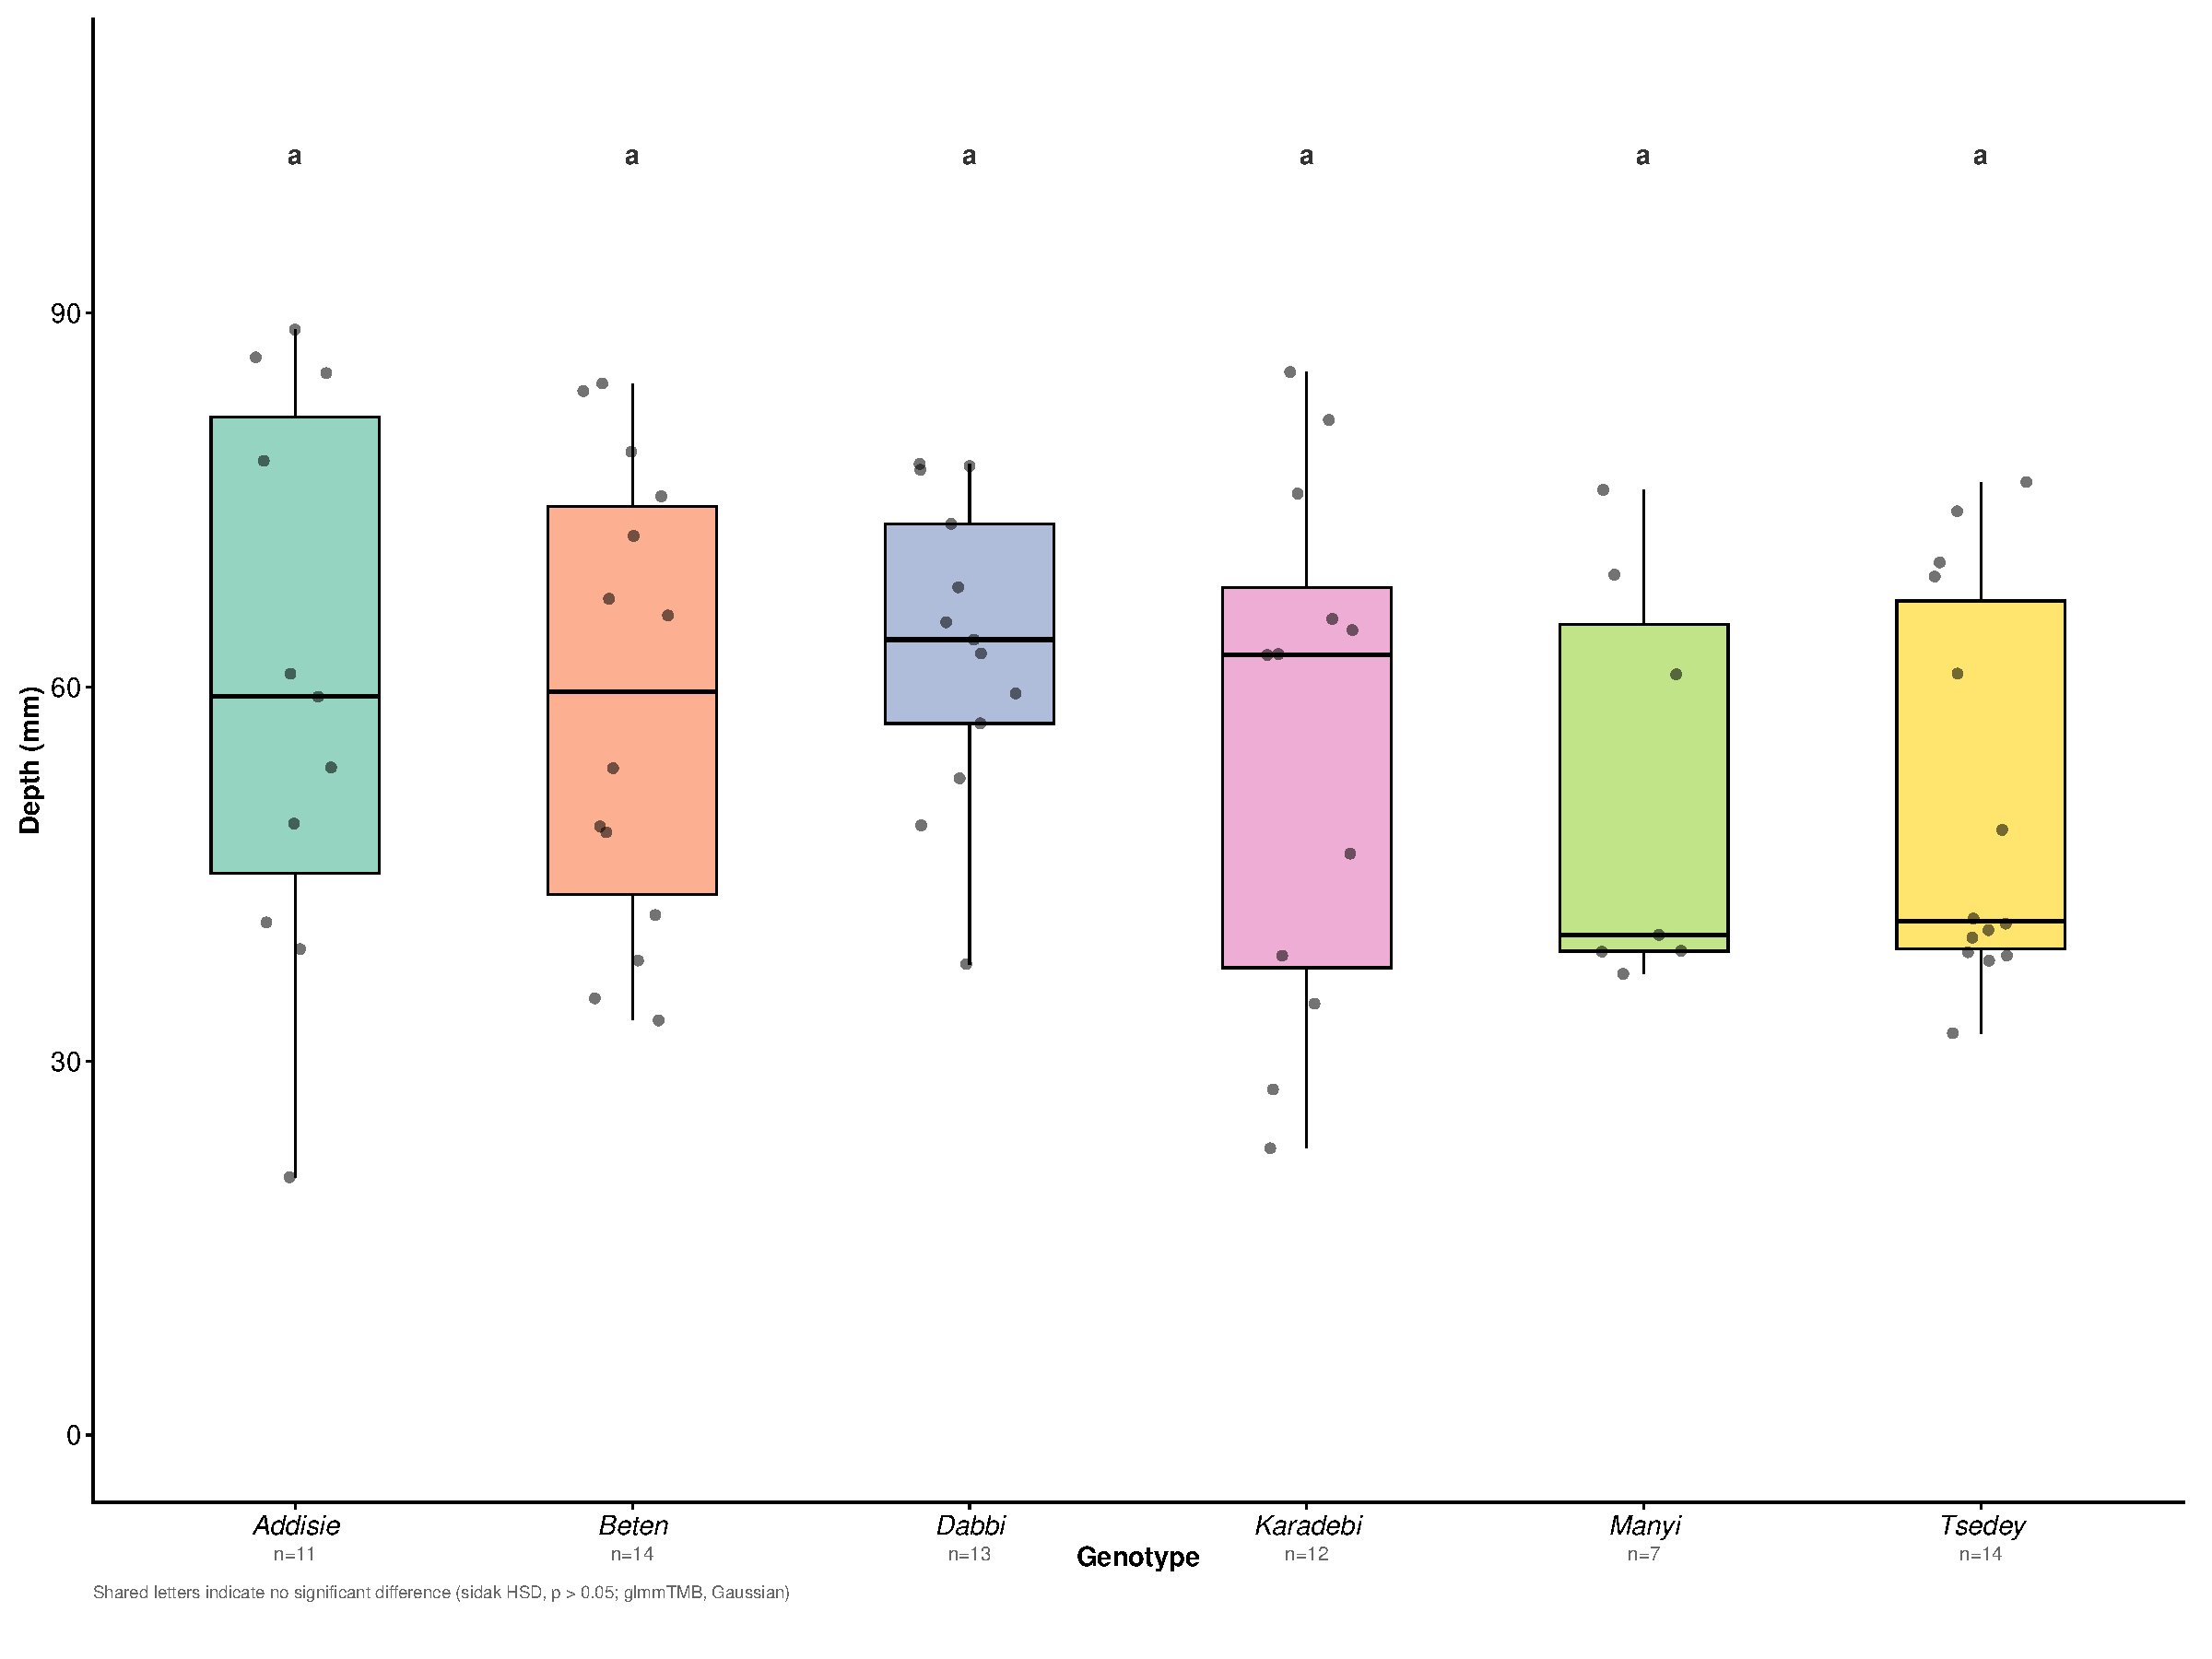
\includegraphics[keepaspectratio]{rsa_day1617_agar_files/figure-pdf/unnamed-chunk-10-6.pdf}}

\subsubsection{Surface area}\label{surface-area}

\begin{Shaded}
\begin{Highlighting}[]
\CommentTok{\# ============================================================}
\CommentTok{\#  Depth Analysis}
\CommentTok{\#  Positive continuous — start raw Gaussian, log if needed}
\CommentTok{\# ============================================================}

\CommentTok{\# ── 1. Inspect distribution ───────────────────────────────────}
\FunctionTok{summary}\NormalTok{(df}\SpecialCharTok{$}\NormalTok{Surface.Area.mm2)}
\end{Highlighting}
\end{Shaded}

\begin{verbatim}
   Min. 1st Qu.  Median    Mean 3rd Qu.    Max. 
  33.44   63.76   95.94  121.87  155.61  510.49 
\end{verbatim}

\begin{Shaded}
\begin{Highlighting}[]
\FunctionTok{hist}\NormalTok{(df}\SpecialCharTok{$}\NormalTok{Surface.Area.mm2, }\AttributeTok{breaks =} \DecValTok{15}\NormalTok{, }\AttributeTok{main =} \StringTok{"Surface Area"}\NormalTok{)}
\end{Highlighting}
\end{Shaded}

\pandocbounded{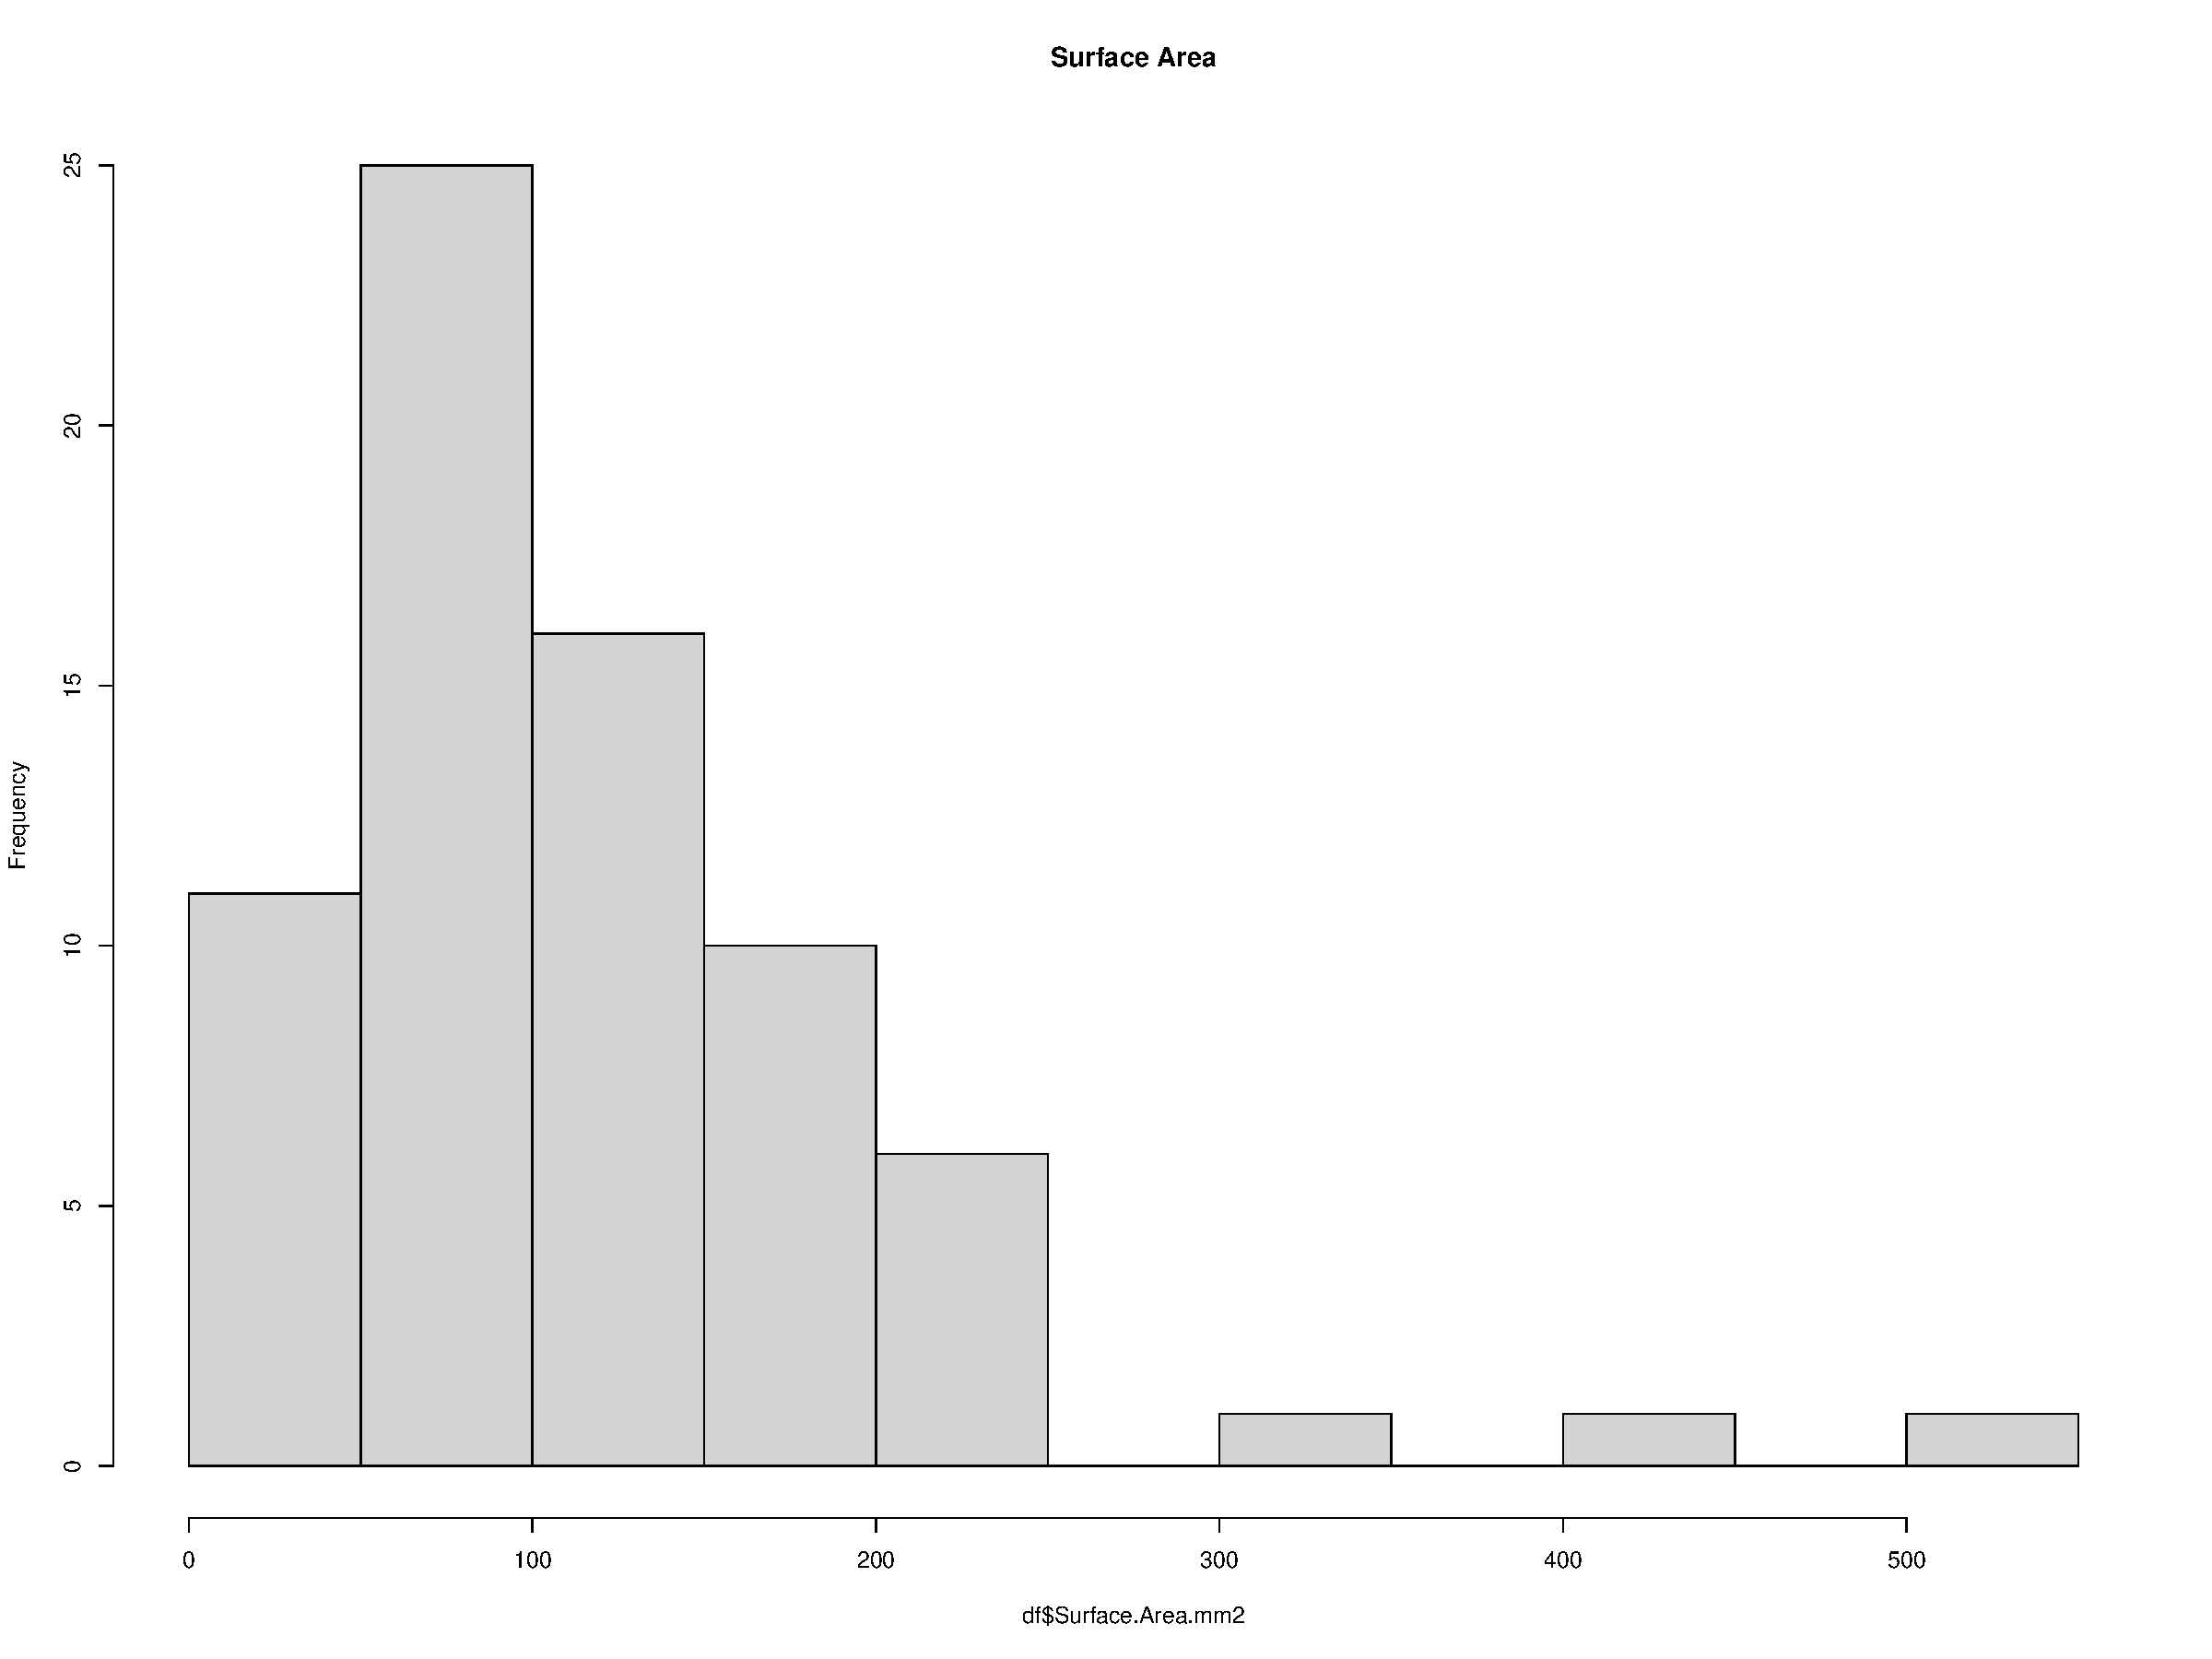
\includegraphics[keepaspectratio]{rsa_day1617_agar_files/figure-pdf/unnamed-chunk-11-1.pdf}}

\begin{Shaded}
\begin{Highlighting}[]
\CommentTok{\# ── 2. Fit full nested model ──────────────────────────────────}
\NormalTok{SA\_full }\OtherTok{\textless{}{-}} \FunctionTok{glmmTMB}\NormalTok{(}
\NormalTok{  Surface.Area.mm2 }\SpecialCharTok{\textasciitilde{}}\NormalTok{ Genotype }\SpecialCharTok{+}\NormalTok{ (}\DecValTok{1} \SpecialCharTok{|}\NormalTok{ Batch}\SpecialCharTok{/}\NormalTok{Plate}\SpecialCharTok{/}\NormalTok{Seed),}
  \AttributeTok{data =}\NormalTok{ df, }\AttributeTok{family =} \FunctionTok{gaussian}\NormalTok{()}
\NormalTok{)}
\end{Highlighting}
\end{Shaded}

\begin{verbatim}
Warning in finalizeTMB(TMBStruc, obj, fit, h, data.tmb.old): Model convergence
problem; non-positive-definite Hessian matrix. See vignette('troubleshooting')
\end{verbatim}

\begin{Shaded}
\begin{Highlighting}[]
\FunctionTok{VarCorr}\NormalTok{(SA\_full)}
\end{Highlighting}
\end{Shaded}

\begin{verbatim}

Conditional model:
 Groups           Name        Std.Dev.  
 Seed:Plate:Batch (Intercept) 1.9069e+01
 Plate:Batch      (Intercept) 4.5635e-04
 Batch            (Intercept) 3.9858e+01
 Residual                     6.5222e+01
\end{verbatim}

\begin{Shaded}
\begin{Highlighting}[]
\FunctionTok{check\_singularity}\NormalTok{(SA\_full)}
\end{Highlighting}
\end{Shaded}

\begin{verbatim}
[1] TRUE
\end{verbatim}

\begin{Shaded}
\begin{Highlighting}[]
\FunctionTok{summary}\NormalTok{(SA\_full)}
\end{Highlighting}
\end{Shaded}

\begin{verbatim}
 Family: gaussian  ( identity )
Formula:          Surface.Area.mm2 ~ Genotype + (1 | Batch/Plate/Seed)
Data: df

      AIC       BIC    logLik -2*log(L)  df.resid 
       NA        NA        NA        NA        61 

Random effects:

Conditional model:
 Groups           Name        Variance  Std.Dev. 
 Seed:Plate:Batch (Intercept) 3.636e+02 1.907e+01
 Plate:Batch      (Intercept) 2.083e-07 4.563e-04
 Batch            (Intercept) 1.589e+03 3.986e+01
 Residual                     4.254e+03 6.522e+01
Number of obs: 71, groups:  Seed:Plate:Batch, 38; Plate:Batch, 18; Batch, 4

Dispersion estimate for gaussian family (sigma^2): 4.25e+03 

Conditional model:
                 Estimate Std. Error z value Pr(>|z|)    
(Intercept)        158.92      29.40   5.406 6.44e-08 ***
GenotypeBeten      -37.40      27.10  -1.380  0.16764    
GenotypeDabbi      -49.73      31.53  -1.577  0.11480    
GenotypeKaradebi   -24.35      30.89  -0.788  0.43053    
GenotypeManyi      -23.25      36.39  -0.639  0.52297    
GenotypeTsedey     -78.11      29.27  -2.669  0.00761 ** 
---
Signif. codes:  0 '***' 0.001 '**' 0.01 '*' 0.05 '.' 0.1 ' ' 1
\end{verbatim}

\begin{Shaded}
\begin{Highlighting}[]
\CommentTok{\# Get Hessian matrix error because plate:batch interaction is very small so will drop this interaction}
\NormalTok{SA\_tmb }\OtherTok{\textless{}{-}} \FunctionTok{glmmTMB}\NormalTok{(}
\NormalTok{  Surface.Area.mm2 }\SpecialCharTok{\textasciitilde{}}\NormalTok{ Genotype }\SpecialCharTok{+}\NormalTok{ (}\DecValTok{1} \SpecialCharTok{|}\NormalTok{ Batch) }\SpecialCharTok{+}\NormalTok{ (}\DecValTok{1} \SpecialCharTok{|}\NormalTok{ Batch}\SpecialCharTok{:}\NormalTok{Plate}\SpecialCharTok{:}\NormalTok{Seed),}
  \AttributeTok{data =}\NormalTok{ df, }\AttributeTok{family =} \FunctionTok{gaussian}\NormalTok{()}
\NormalTok{)}
\end{Highlighting}
\end{Shaded}

\begin{verbatim}
Warning in finalizeTMB(TMBStruc, obj, fit, h, data.tmb.old): Model convergence
problem; non-positive-definite Hessian matrix. See vignette('troubleshooting')
\end{verbatim}

\begin{Shaded}
\begin{Highlighting}[]
\FunctionTok{VarCorr}\NormalTok{(SA\_tmb)}
\end{Highlighting}
\end{Shaded}

\begin{verbatim}

Conditional model:
 Groups           Name        Std.Dev.
 Batch            (Intercept) 41.96691
 Batch:Plate:Seed (Intercept)  0.25849
 Residual                     67.62096
\end{verbatim}

\begin{Shaded}
\begin{Highlighting}[]
\FunctionTok{check\_singularity}\NormalTok{(SA\_tmb)}
\end{Highlighting}
\end{Shaded}

\begin{verbatim}
[1] FALSE
\end{verbatim}

\begin{Shaded}
\begin{Highlighting}[]
\FunctionTok{summary}\NormalTok{(SA\_tmb)}
\end{Highlighting}
\end{Shaded}

\begin{verbatim}
 Family: gaussian  ( identity )
Formula:          
Surface.Area.mm2 ~ Genotype + (1 | Batch) + (1 | Batch:Plate:Seed)
Data: df

      AIC       BIC    logLik -2*log(L)  df.resid 
       NA        NA        NA        NA        62 

Random effects:

Conditional model:
 Groups           Name        Variance  Std.Dev.
 Batch            (Intercept) 1.761e+03 41.9669 
 Batch:Plate:Seed (Intercept) 6.682e-02  0.2585 
 Residual                     4.573e+03 67.6210 
Number of obs: 71, groups:  Batch, 4; Batch:Plate:Seed, 38

Dispersion estimate for gaussian family (sigma^2): 4.57e+03 

Conditional model:
                 Estimate Std. Error z value Pr(>|z|)    
(Intercept)        156.53      29.92   5.232 1.68e-07 ***
GenotypeBeten      -35.29      27.51  -1.283   0.1996    
GenotypeDabbi      -47.41      31.61  -1.500   0.1336    
GenotypeKaradebi   -22.18      31.24  -0.710   0.4777    
GenotypeManyi      -18.12      36.11  -0.502   0.6159    
GenotypeTsedey     -74.14      29.07  -2.550   0.0108 *  
---
Signif. codes:  0 '***' 0.001 '**' 0.01 '*' 0.05 '.' 0.1 ' ' 1
\end{verbatim}

\begin{Shaded}
\begin{Highlighting}[]
\CommentTok{\# Still getting error so dropping the batch:plate:seed interaction}
\NormalTok{SA\_tmb }\OtherTok{\textless{}{-}} \FunctionTok{glmmTMB}\NormalTok{(}
\NormalTok{  Surface.Area.mm2 }\SpecialCharTok{\textasciitilde{}}\NormalTok{ Genotype }\SpecialCharTok{+}\NormalTok{ (}\DecValTok{1} \SpecialCharTok{|}\NormalTok{ Batch),}
  \AttributeTok{data =}\NormalTok{ df, }\AttributeTok{family =} \FunctionTok{gaussian}\NormalTok{()}
\NormalTok{)}

\FunctionTok{VarCorr}\NormalTok{(SA\_tmb)}
\end{Highlighting}
\end{Shaded}

\begin{verbatim}

Conditional model:
 Groups   Name        Std.Dev.
 Batch    (Intercept) 41.965  
 Residual             67.622  
\end{verbatim}

\begin{Shaded}
\begin{Highlighting}[]
\FunctionTok{check\_singularity}\NormalTok{(SA\_tmb)}
\end{Highlighting}
\end{Shaded}

\begin{verbatim}
[1] FALSE
\end{verbatim}

\begin{Shaded}
\begin{Highlighting}[]
\FunctionTok{summary}\NormalTok{(SA\_tmb)}
\end{Highlighting}
\end{Shaded}

\begin{verbatim}
 Family: gaussian  ( identity )
Formula:          Surface.Area.mm2 ~ Genotype + (1 | Batch)
Data: df

      AIC       BIC    logLik -2*log(L)  df.resid 
    824.1     842.2    -404.0     808.1        63 

Random effects:

Conditional model:
 Groups   Name        Variance Std.Dev.
 Batch    (Intercept) 1761     41.97   
 Residual             4573     67.62   
Number of obs: 71, groups:  Batch, 4

Dispersion estimate for gaussian family (sigma^2): 4.57e+03 

Conditional model:
                 Estimate Std. Error z value Pr(>|z|)    
(Intercept)        156.52      29.92   5.232 1.68e-07 ***
GenotypeBeten      -35.29      27.51  -1.283   0.1996    
GenotypeDabbi      -47.41      31.61  -1.500   0.1336    
GenotypeKaradebi   -22.18      31.24  -0.710   0.4777    
GenotypeManyi      -18.11      36.11  -0.502   0.6159    
GenotypeTsedey     -74.14      29.07  -2.550   0.0108 *  
---
Signif. codes:  0 '***' 0.001 '**' 0.01 '*' 0.05 '.' 0.1 ' ' 1
\end{verbatim}

\begin{Shaded}
\begin{Highlighting}[]
\NormalTok{sim\_res }\OtherTok{\textless{}{-}} \FunctionTok{simulateResiduals}\NormalTok{(SA\_tmb, }\AttributeTok{n =} \DecValTok{1000}\NormalTok{)}
\FunctionTok{plot}\NormalTok{(sim\_res)}
\end{Highlighting}
\end{Shaded}

\pandocbounded{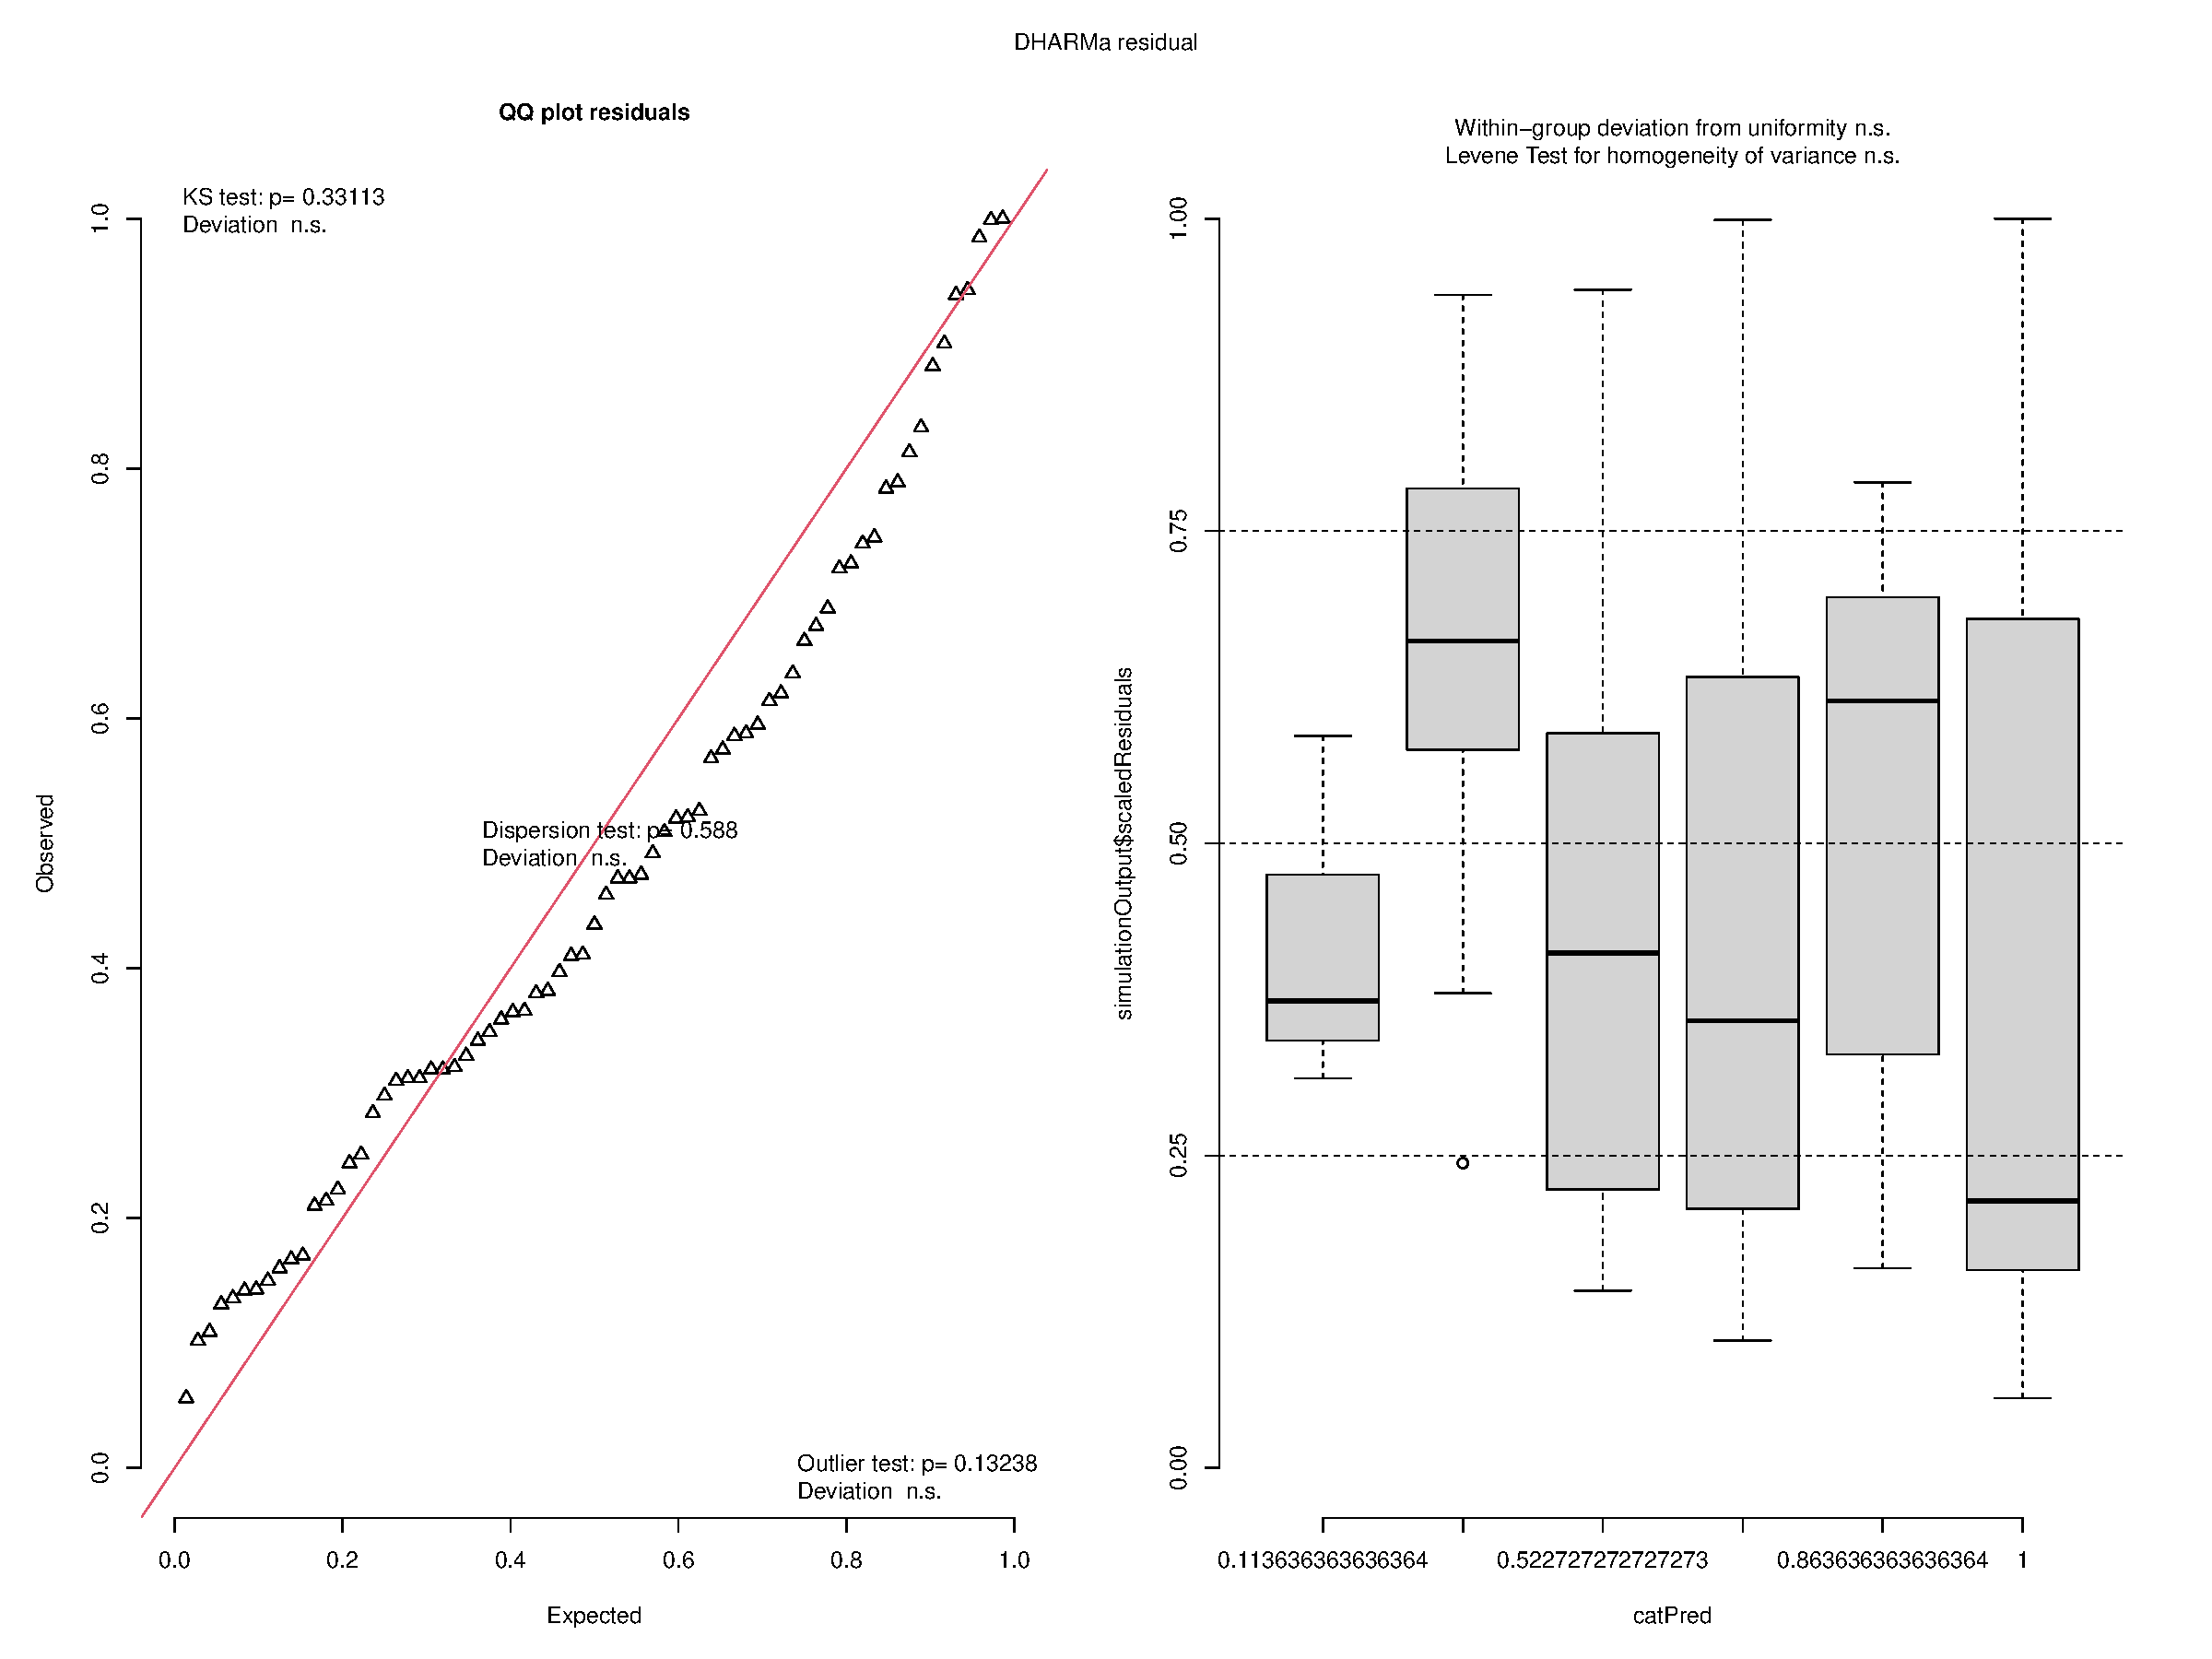
\includegraphics[keepaspectratio]{rsa_day1617_agar_files/figure-pdf/unnamed-chunk-11-2.pdf}}

\begin{Shaded}
\begin{Highlighting}[]
\FunctionTok{testUniformity}\NormalTok{(sim\_res)                     }\CommentTok{\# p \textgreater{} 0.05 = raw Gaussian fine}
\end{Highlighting}
\end{Shaded}

\pandocbounded{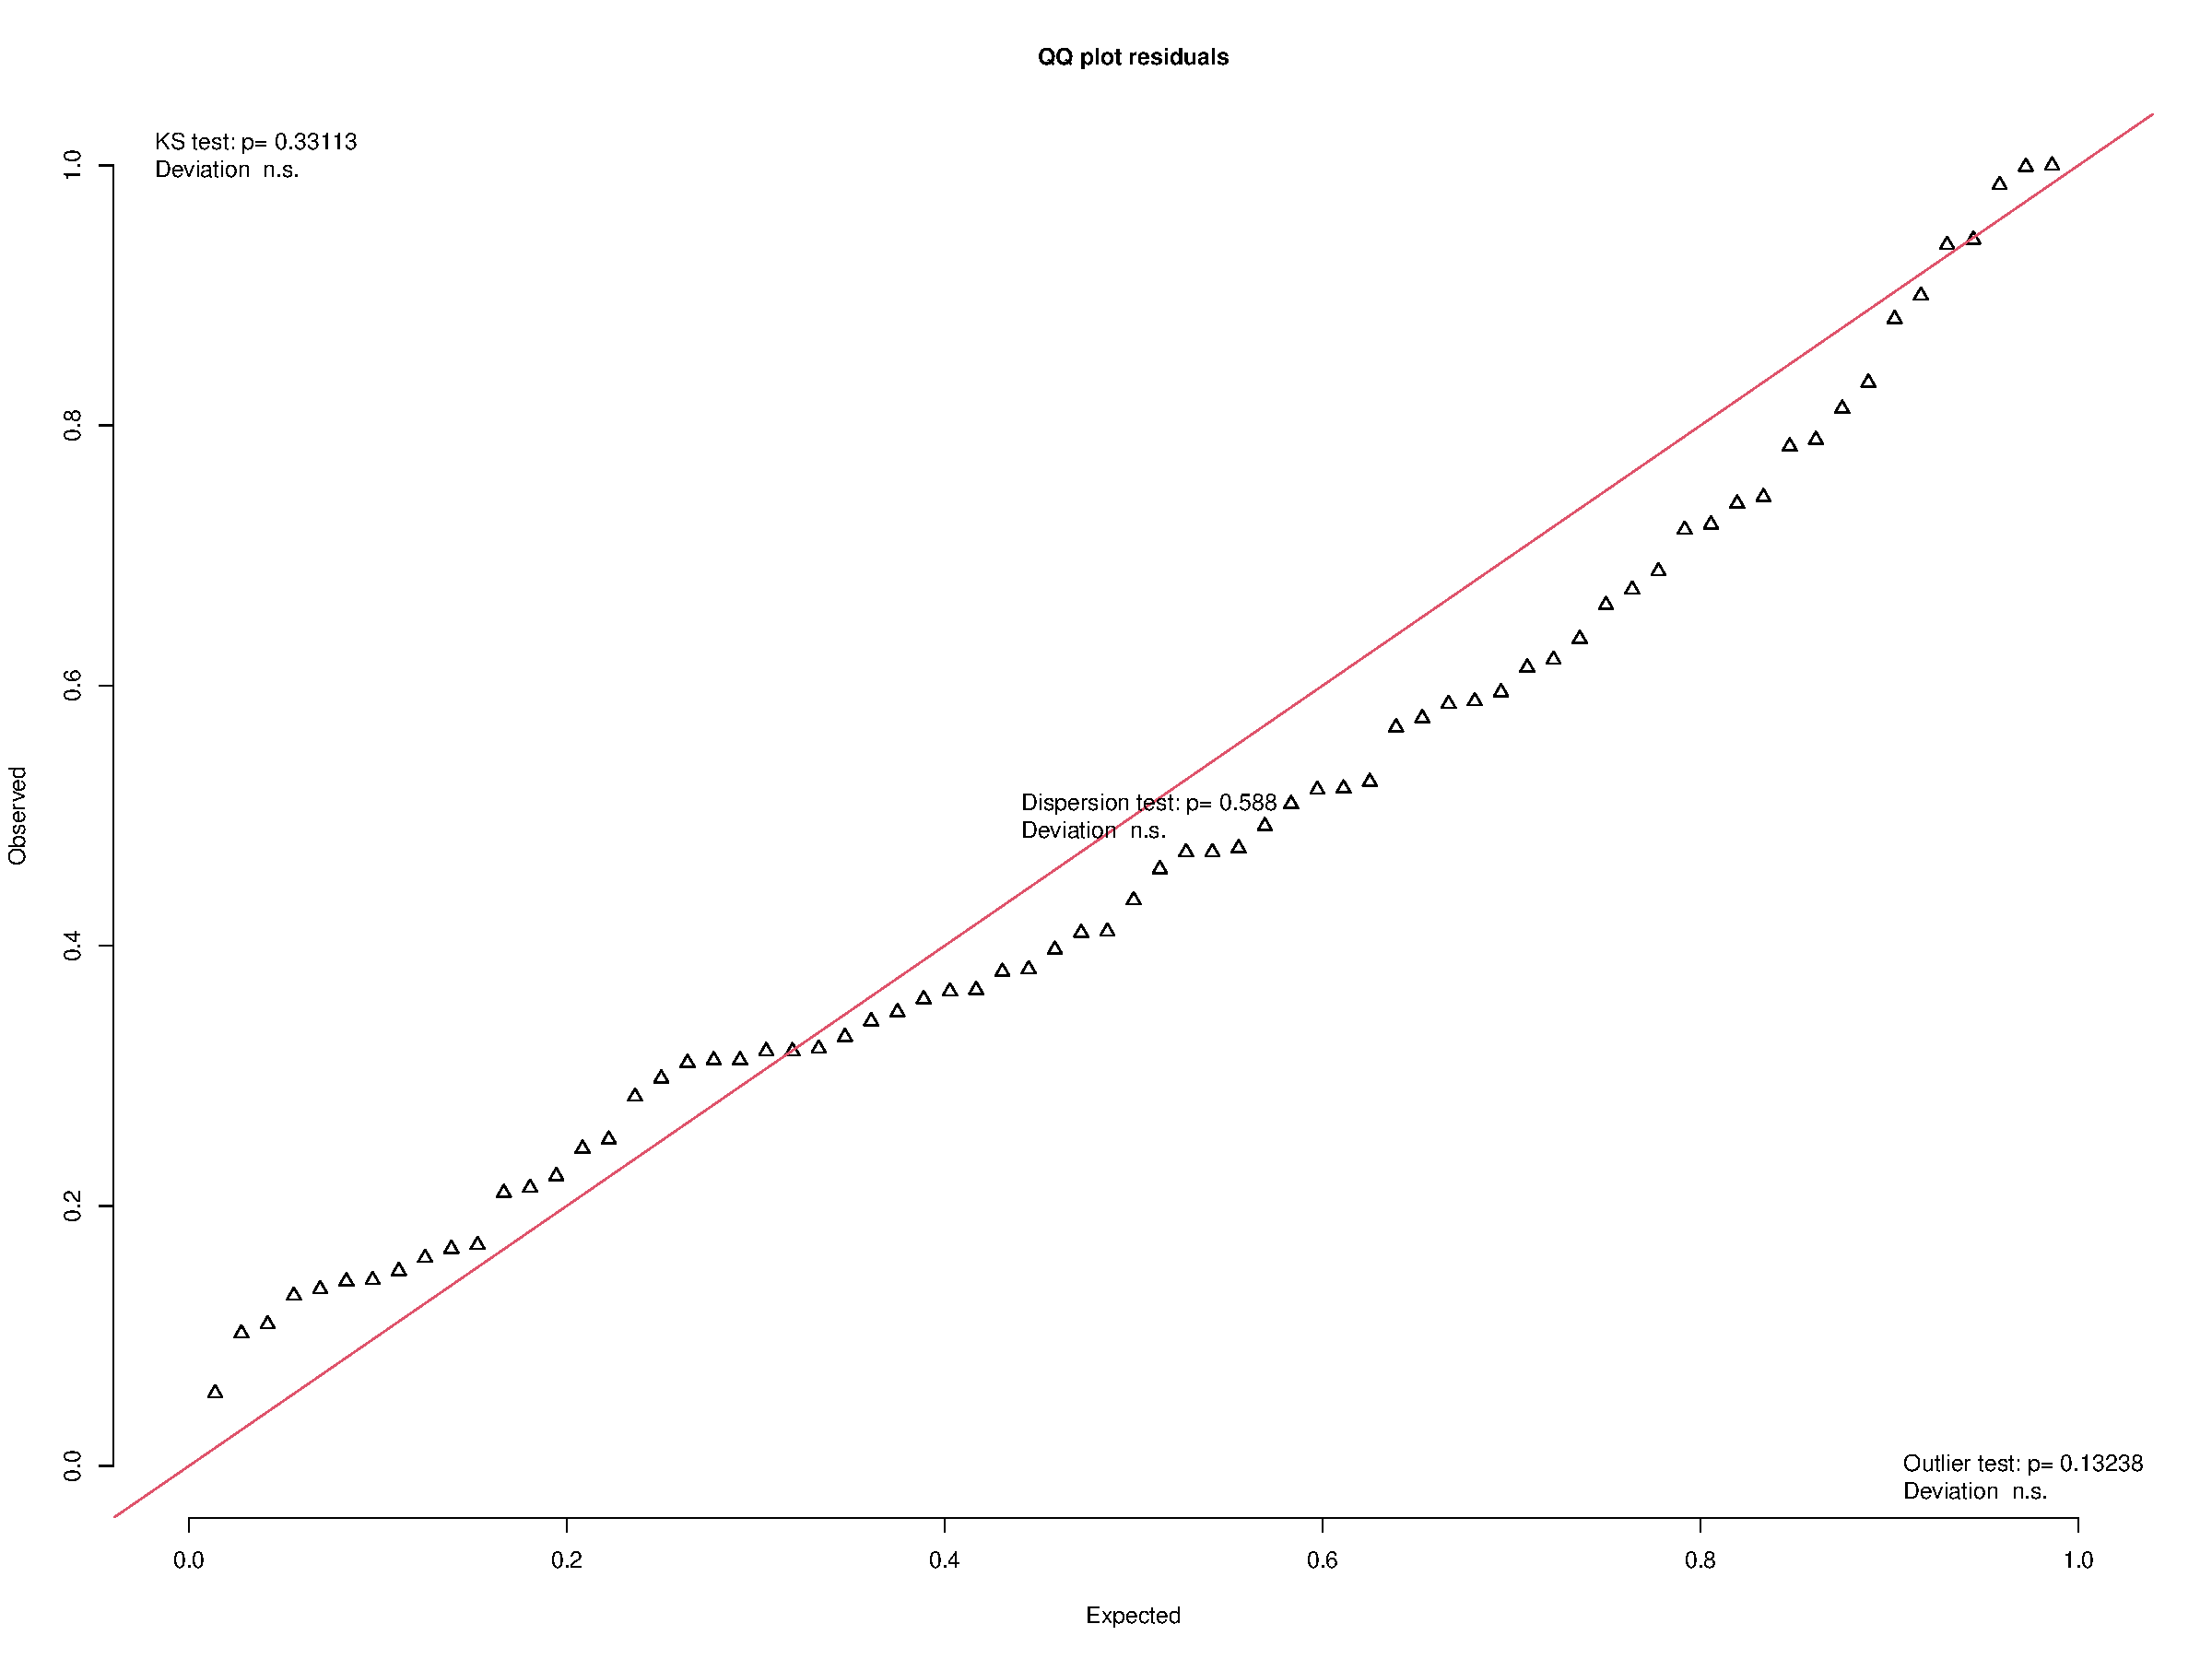
\includegraphics[keepaspectratio]{rsa_day1617_agar_files/figure-pdf/unnamed-chunk-11-3.pdf}}

\begin{verbatim}

    Asymptotic one-sample Kolmogorov-Smirnov test

data:  simulationOutput$scaledResiduals
D = 0.11239, p-value = 0.3311
alternative hypothesis: two-sided
\end{verbatim}

\begin{Shaded}
\begin{Highlighting}[]
\FunctionTok{testDispersion}\NormalTok{(sim\_res)                     }\CommentTok{\# ratio ≈ 1.0}
\end{Highlighting}
\end{Shaded}

\pandocbounded{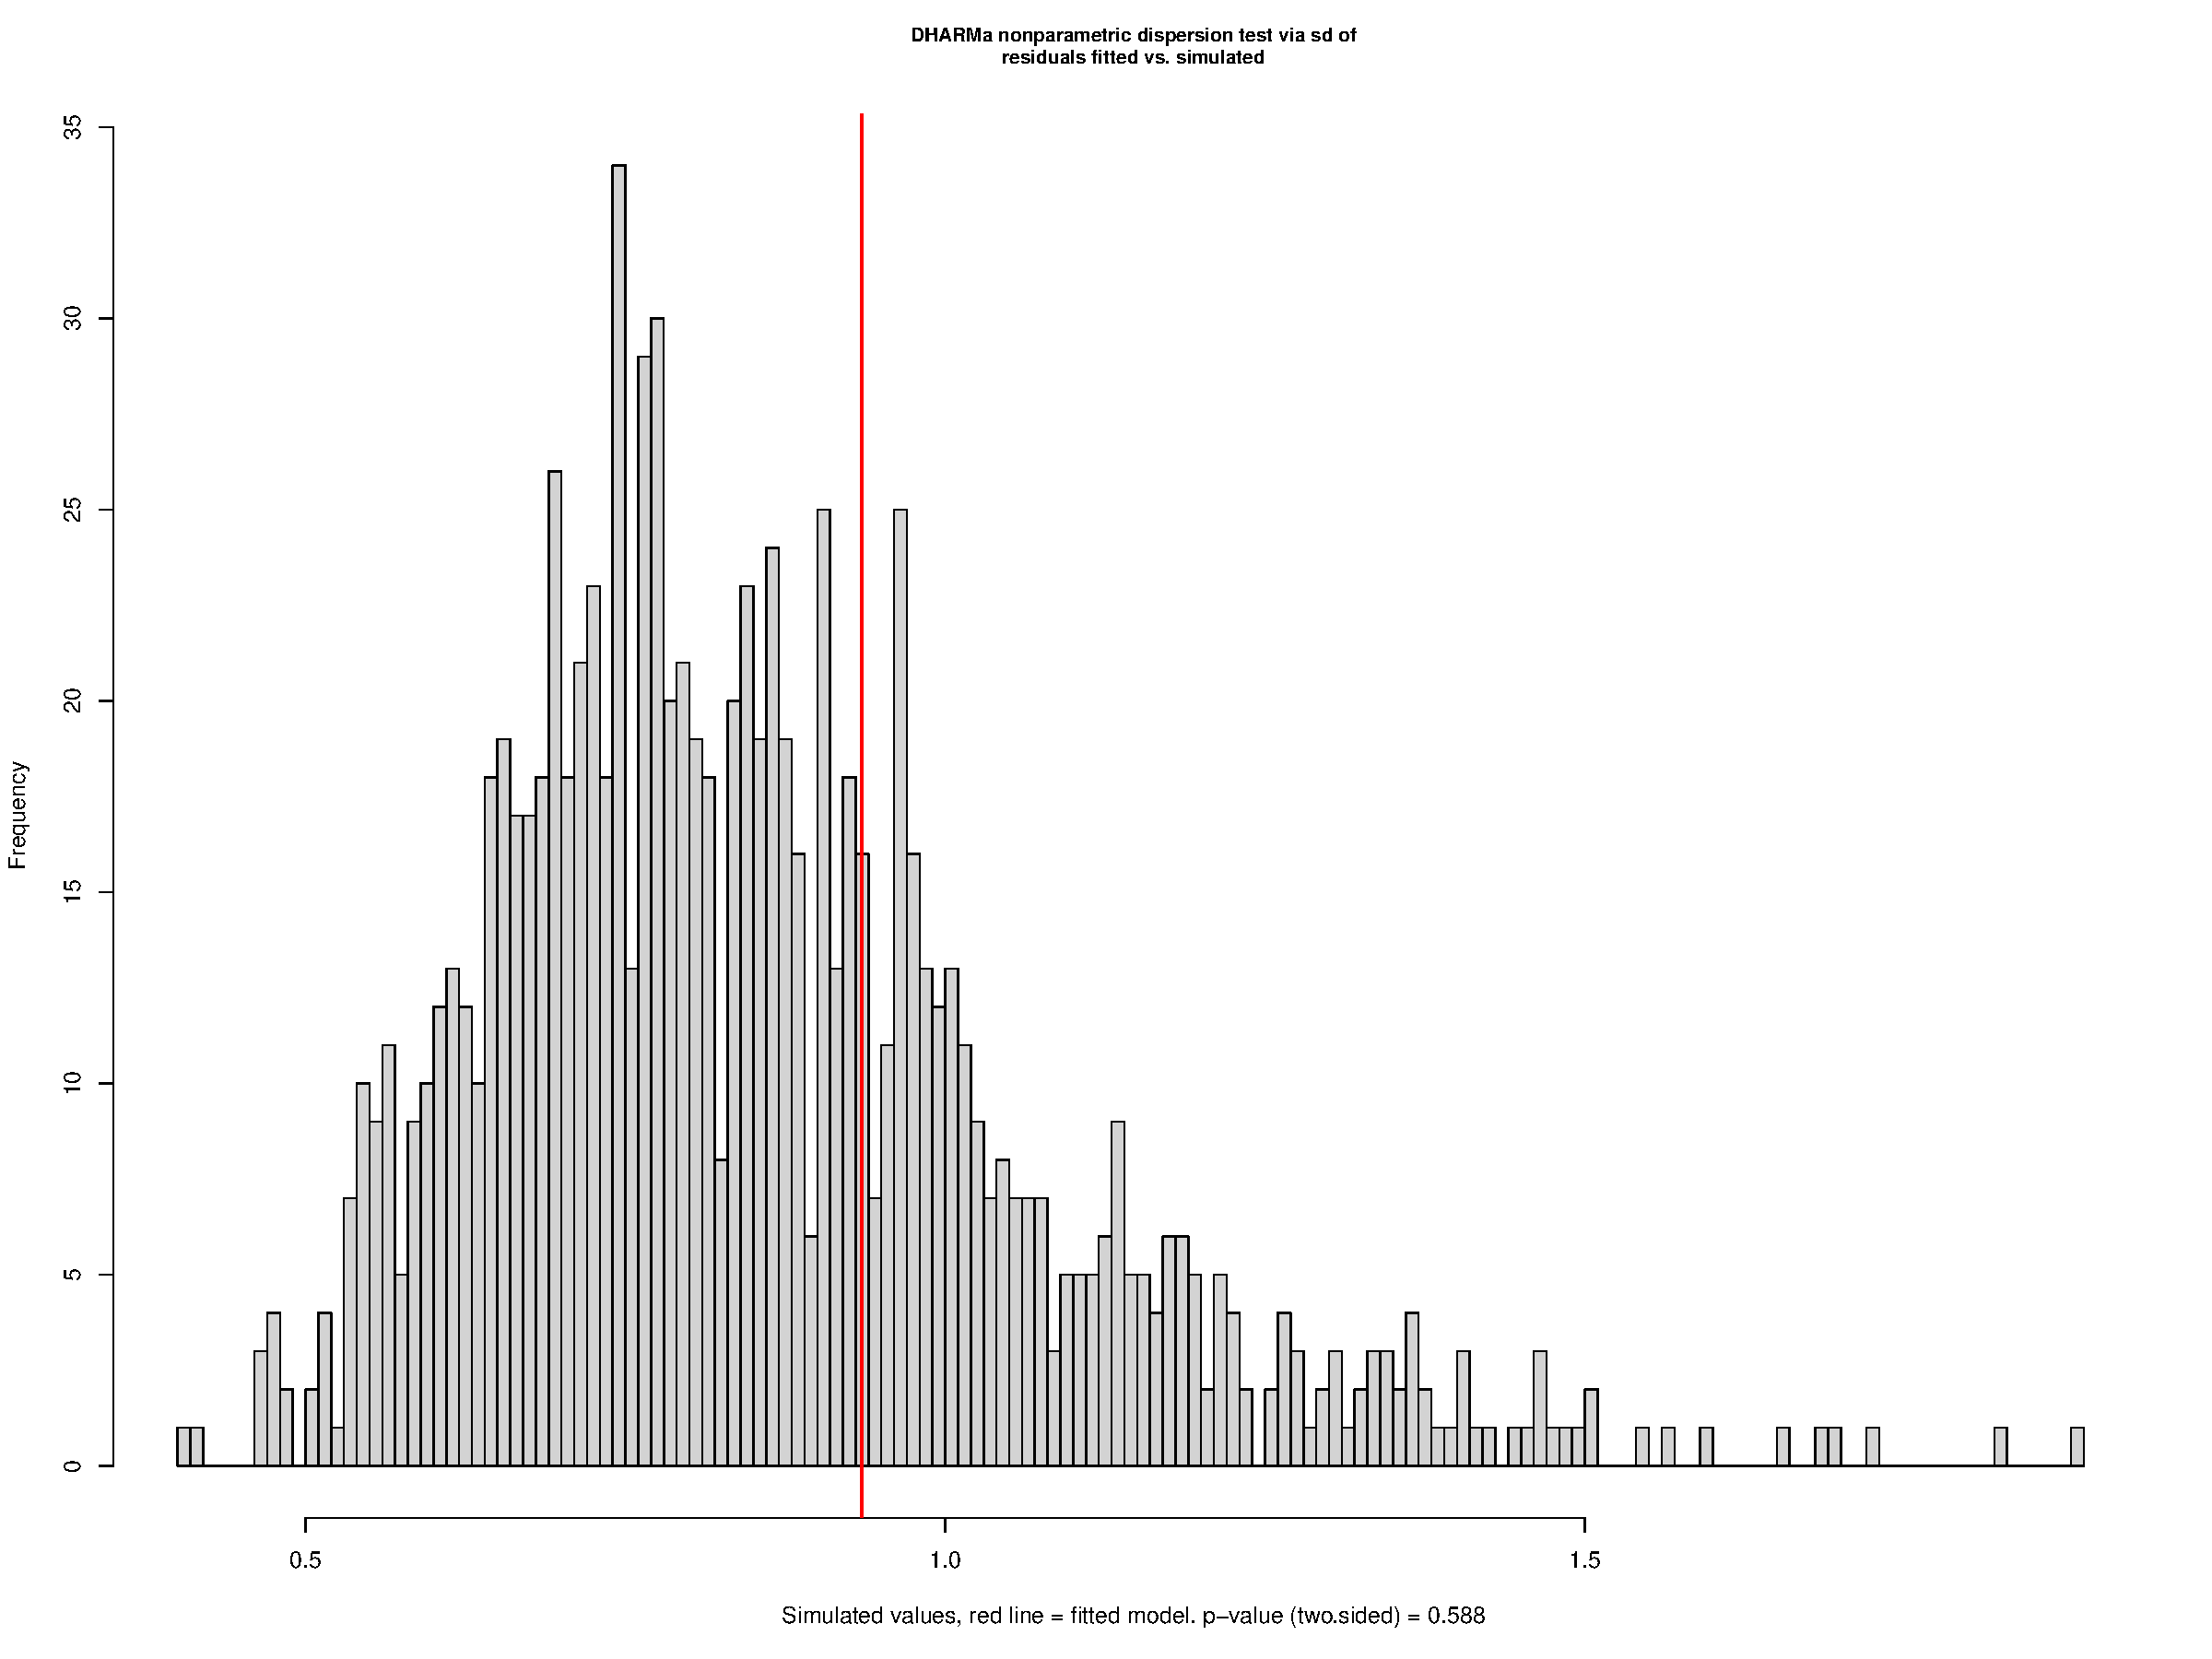
\includegraphics[keepaspectratio]{rsa_day1617_agar_files/figure-pdf/unnamed-chunk-11-4.pdf}}

\begin{verbatim}

    DHARMa nonparametric dispersion test via sd of residuals fitted vs.
    simulated

data:  simulationOutput
dispersion = 1.0918, p-value = 0.588
alternative hypothesis: two.sided
\end{verbatim}

\begin{Shaded}
\begin{Highlighting}[]
\FunctionTok{plotResiduals}\NormalTok{(sim\_res, }\AttributeTok{form =}\NormalTok{ df}\SpecialCharTok{$}\NormalTok{Genotype)}
\end{Highlighting}
\end{Shaded}

\pandocbounded{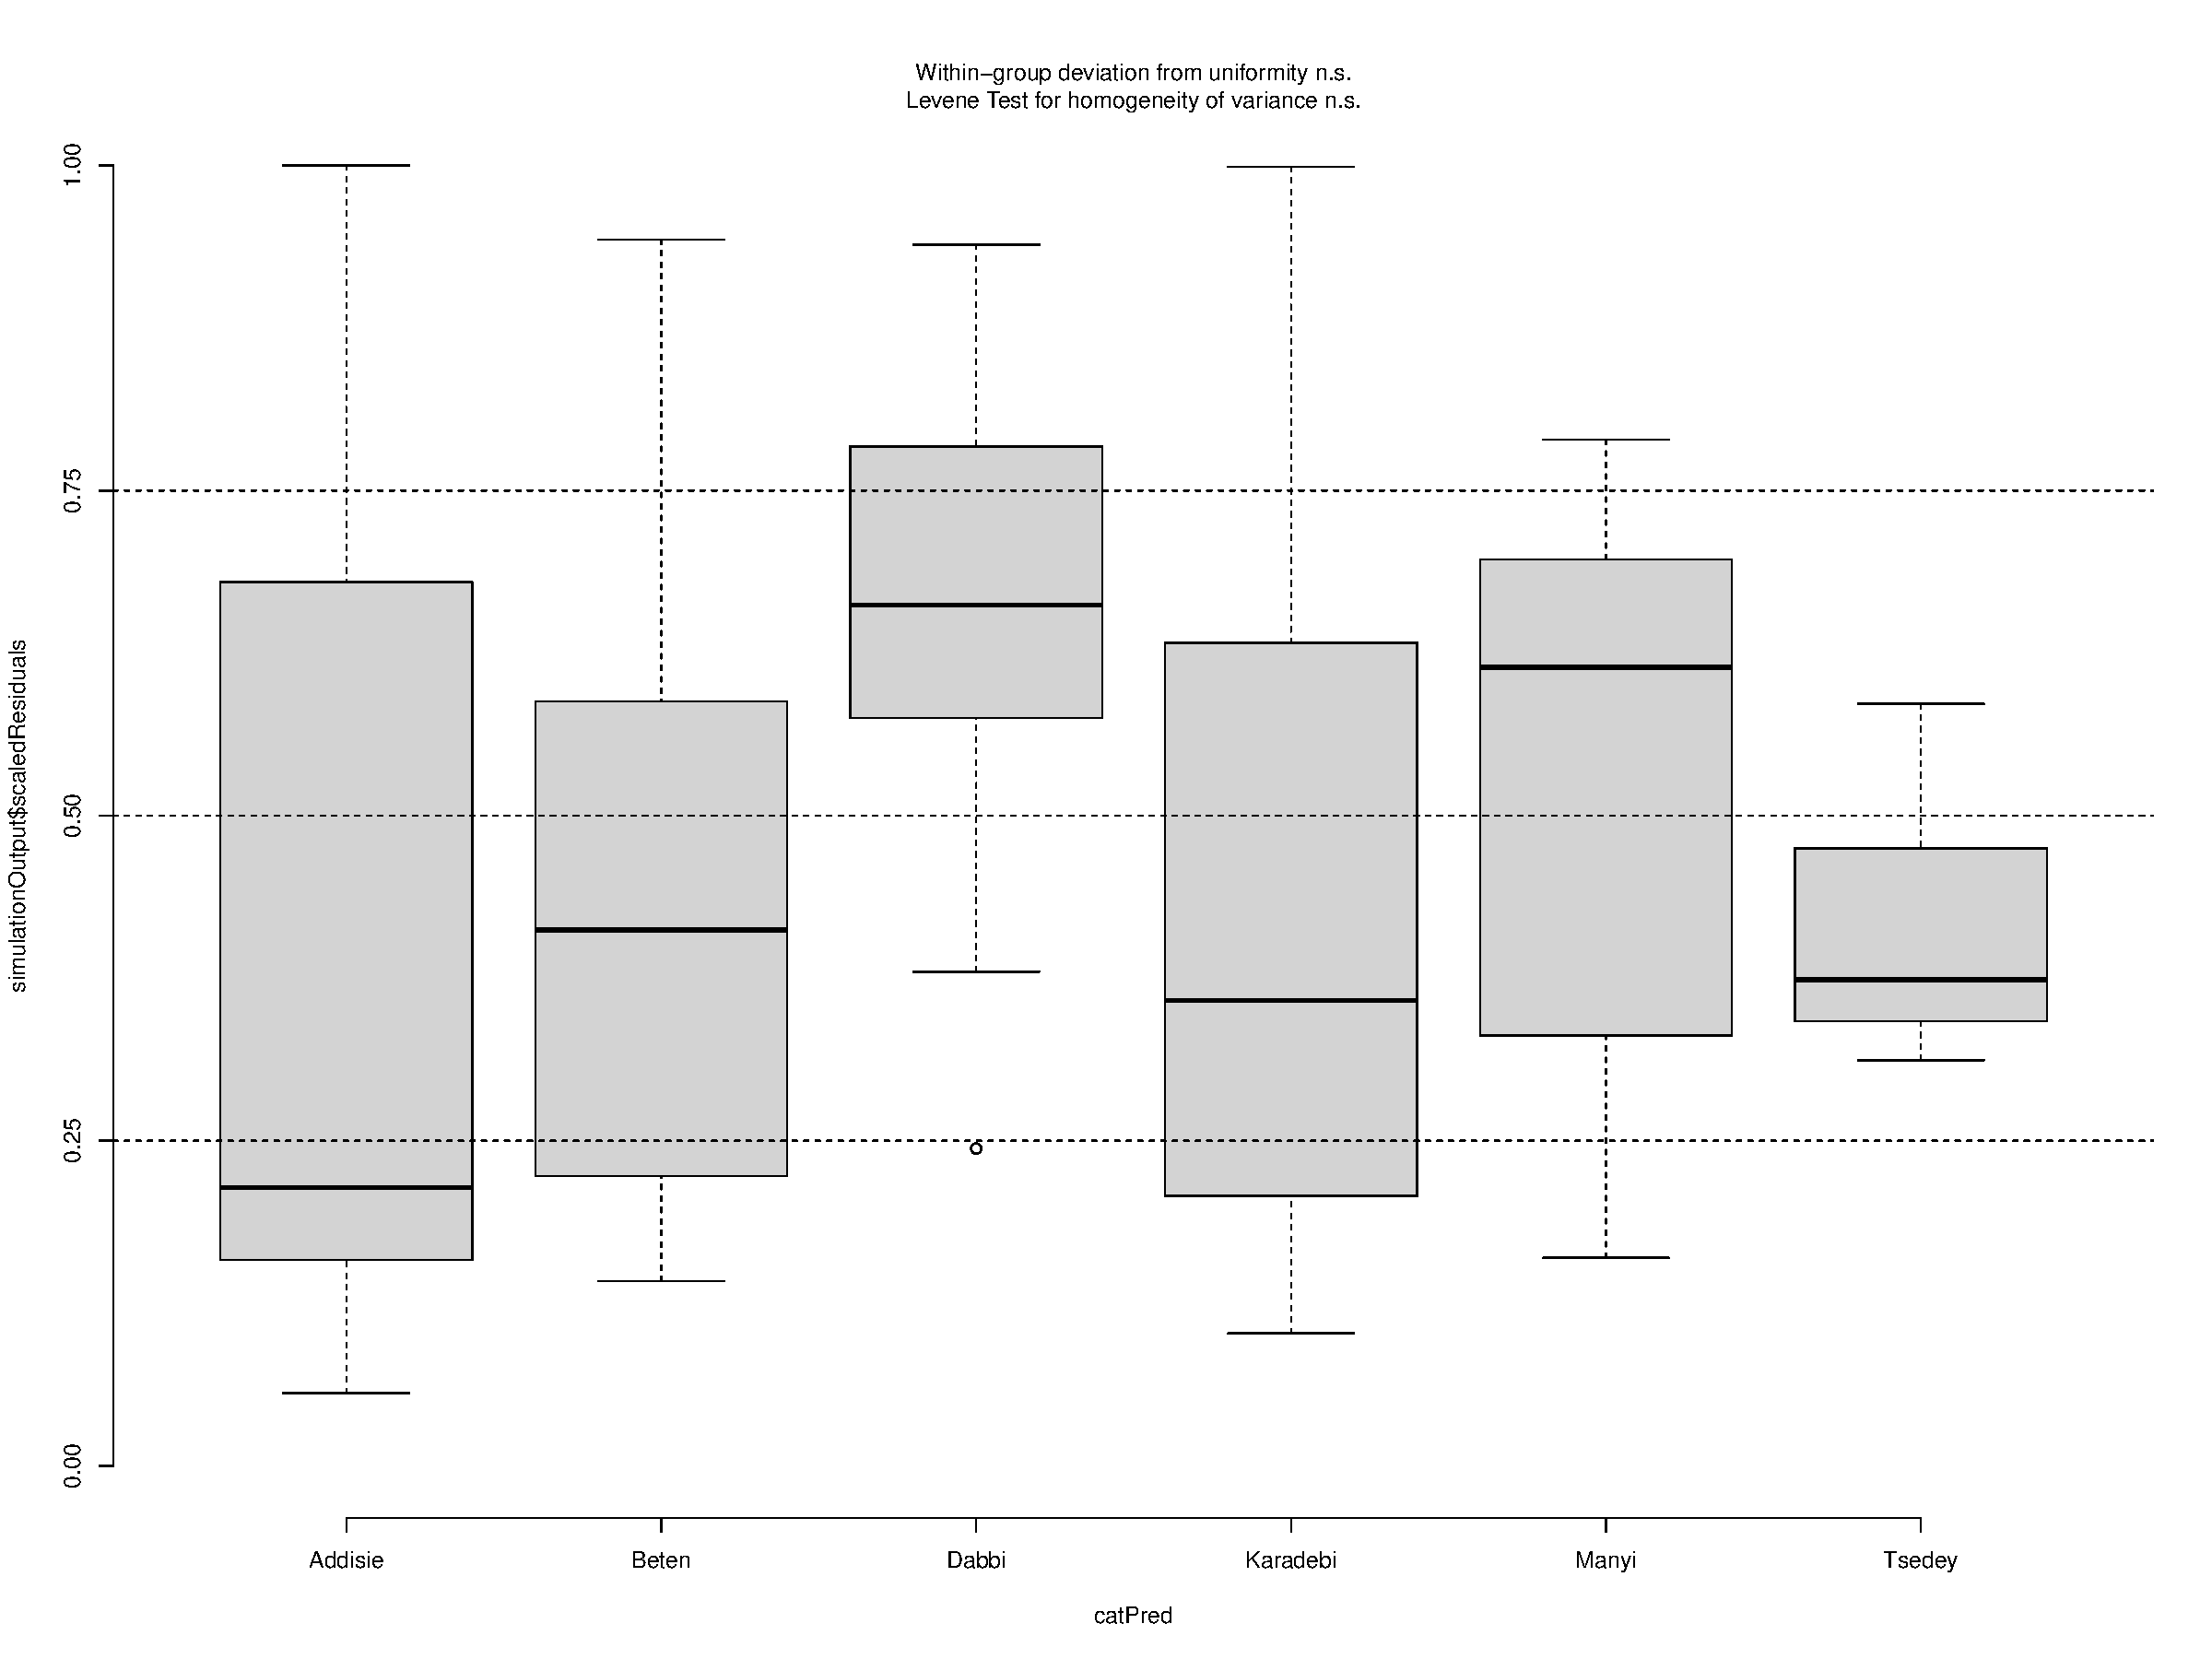
\includegraphics[keepaspectratio]{rsa_day1617_agar_files/figure-pdf/unnamed-chunk-11-5.pdf}}

\begin{Shaded}
\begin{Highlighting}[]
\CommentTok{\# fit is pretty good so happy to continue }

\CommentTok{\# ── 5. Test overall Genotype effect ──────────────────────────}
\NormalTok{car}\SpecialCharTok{::}\FunctionTok{Anova}\NormalTok{(SA\_tmb, }\AttributeTok{type =} \StringTok{"III"}\NormalTok{)}
\end{Highlighting}
\end{Shaded}

\begin{verbatim}
Analysis of Deviance Table (Type III Wald chisquare tests)

Response: Surface.Area.mm2
              Chisq Df Pr(>Chisq)    
(Intercept) 27.3699  1   1.68e-07 ***
Genotype     8.2686  5      0.142    
---
Signif. codes:  0 '***' 0.001 '**' 0.01 '*' 0.05 '.' 0.1 ' ' 1
\end{verbatim}

\begin{Shaded}
\begin{Highlighting}[]
\CommentTok{\# ── 6. Pairwise comparisons + CLD ────────────────────────────}
\NormalTok{emm }\OtherTok{\textless{}{-}} \FunctionTok{emmeans}\NormalTok{(SA\_tmb, }\SpecialCharTok{\textasciitilde{}}\NormalTok{ Genotype)}
\FunctionTok{pairs}\NormalTok{(emm, }\AttributeTok{adjust =} \StringTok{"sidak"}\NormalTok{)}
\end{Highlighting}
\end{Shaded}

\begin{verbatim}
 contrast           estimate   SE  df z.ratio p.value
 Addisie - Beten       35.29 27.5 Inf   1.283  0.9645
 Addisie - Dabbi       47.41 31.6 Inf   1.500  0.8837
 Addisie - Karadebi    22.18 31.2 Inf   0.710  0.9999
 Addisie - Manyi       18.11 36.1 Inf   0.502  1.0000
 Addisie - Tsedey      74.14 29.1 Inf   2.550  0.1499
 Beten - Dabbi         12.11 31.1 Inf   0.389  1.0000
 Beten - Karadebi     -13.12 29.6 Inf  -0.443  1.0000
 Beten - Manyi        -17.18 34.6 Inf  -0.496  1.0000
 Beten - Tsedey        38.85 27.0 Inf   1.438  0.9135
 Dabbi - Karadebi     -25.23 28.6 Inf  -0.882  0.9992
 Dabbi - Manyi        -29.29 33.4 Inf  -0.878  0.9992
 Dabbi - Tsedey        26.73 31.0 Inf   0.861  0.9994
 Karadebi - Manyi      -4.06 32.7 Inf  -0.124  1.0000
 Karadebi - Tsedey     51.96 29.7 Inf   1.747  0.7164
 Manyi - Tsedey        56.02 33.2 Inf   1.686  0.7638

P value adjustment: sidak method for 15 tests 
\end{verbatim}

\begin{Shaded}
\begin{Highlighting}[]
\NormalTok{cld\_df }\OtherTok{\textless{}{-}} \FunctionTok{as.data.frame}\NormalTok{(}\FunctionTok{cld}\NormalTok{(emm, }\AttributeTok{adjust =} \StringTok{"sidak"}\NormalTok{,}
                             \AttributeTok{Letters =}\NormalTok{ letters, }\AttributeTok{alpha =} \FloatTok{0.05}\NormalTok{)) }\SpecialCharTok{\%\textgreater{}\%}
  \FunctionTok{mutate}\NormalTok{(}\AttributeTok{.group =} \FunctionTok{trimws}\NormalTok{(.group))}

\NormalTok{n\_df }\OtherTok{\textless{}{-}}\NormalTok{ df }\SpecialCharTok{\%\textgreater{}\%}
  \FunctionTok{count}\NormalTok{(Genotype) }\SpecialCharTok{\%\textgreater{}\%}
  \FunctionTok{mutate}\NormalTok{(}\AttributeTok{label =} \FunctionTok{paste0}\NormalTok{(}\StringTok{"n="}\NormalTok{, n))}


\CommentTok{\# ── 7. Plot 1 — Boxplot ───────────────────────────────────────}

\NormalTok{y\_ceil }\OtherTok{\textless{}{-}} \FunctionTok{max}\NormalTok{(df}\SpecialCharTok{$}\NormalTok{Surface.Area.mm2) }\SpecialCharTok{*} \FloatTok{1.22}
\NormalTok{y\_label }\OtherTok{\textless{}{-}}\NormalTok{ y\_ceil }\SpecialCharTok{*} \FloatTok{0.95}

\NormalTok{p1 }\OtherTok{\textless{}{-}} \FunctionTok{ggplot}\NormalTok{(df, }\FunctionTok{aes}\NormalTok{(}\AttributeTok{x =}\NormalTok{ Genotype, }\AttributeTok{y =}\NormalTok{ Surface.Area.mm2, }\AttributeTok{fill =}\NormalTok{ Genotype)) }\SpecialCharTok{+}

  \FunctionTok{geom\_boxplot}\NormalTok{(}
    \AttributeTok{alpha         =} \FloatTok{0.7}\NormalTok{,}
    \AttributeTok{outlier.shape =} \ConstantTok{NA}\NormalTok{,}
    \AttributeTok{width         =} \FloatTok{0.5}\NormalTok{,}
    \AttributeTok{colour        =} \StringTok{"black"}\NormalTok{,}
    \AttributeTok{linewidth     =} \FloatTok{0.5}
\NormalTok{  ) }\SpecialCharTok{+}

  \FunctionTok{geom\_jitter}\NormalTok{(}
    \AttributeTok{width  =} \FloatTok{0.15}\NormalTok{,}
    \AttributeTok{size   =} \FloatTok{1.8}\NormalTok{,}
    \AttributeTok{alpha  =} \FloatTok{0.55}\NormalTok{,}
    \AttributeTok{colour =} \StringTok{"black"}
\NormalTok{  ) }\SpecialCharTok{+}

  \FunctionTok{geom\_text}\NormalTok{(}
    \AttributeTok{data        =}\NormalTok{ cld\_df,}
    \FunctionTok{aes}\NormalTok{(}\AttributeTok{x =}\NormalTok{ Genotype, }\AttributeTok{label =}\NormalTok{ .group),}
    \AttributeTok{y           =}\NormalTok{ y\_label,}
    \AttributeTok{inherit.aes =} \ConstantTok{FALSE}\NormalTok{,}
    \AttributeTok{size        =} \DecValTok{5}\NormalTok{,}
    \AttributeTok{fontface    =} \StringTok{"bold"}\NormalTok{,}
    \AttributeTok{colour      =} \StringTok{"grey20"}
\NormalTok{  ) }\SpecialCharTok{+}

  \FunctionTok{geom\_text}\NormalTok{(}
    \AttributeTok{data        =}\NormalTok{ n\_df,}
    \FunctionTok{aes}\NormalTok{(}\AttributeTok{x =}\NormalTok{ Genotype, }\AttributeTok{label =}\NormalTok{ label),}
    \AttributeTok{y           =} \SpecialCharTok{{-}}\ConstantTok{Inf}\NormalTok{,}
    \AttributeTok{vjust       =} \FloatTok{4.2}\NormalTok{,}
    \AttributeTok{inherit.aes =} \ConstantTok{FALSE}\NormalTok{,}
    \AttributeTok{size        =} \FloatTok{3.5}\NormalTok{,}
    \AttributeTok{colour      =} \StringTok{"grey40"}
\NormalTok{  ) }\SpecialCharTok{+}

  \FunctionTok{scale\_fill\_brewer}\NormalTok{(}\AttributeTok{palette =} \StringTok{"Set2"}\NormalTok{) }\SpecialCharTok{+}

  \FunctionTok{labs}\NormalTok{(}
    \AttributeTok{x       =} \StringTok{"Genotype"}\NormalTok{,}
    \AttributeTok{y       =} \StringTok{"Surface Area (mm)"}\NormalTok{,}
    \AttributeTok{caption =} \StringTok{"Shared letters indicate no significant difference (sidak HSD, p \textgreater{} 0.05; glmmTMB, Gaussian)"}
\NormalTok{  ) }\SpecialCharTok{+}

  \FunctionTok{theme\_classic}\NormalTok{(}\AttributeTok{base\_size =} \DecValTok{14}\NormalTok{) }\SpecialCharTok{+}
  \FunctionTok{theme}\NormalTok{(}
    \AttributeTok{legend.position =} \StringTok{"none"}\NormalTok{,}
    \AttributeTok{axis.line       =} \FunctionTok{element\_line}\NormalTok{(}\AttributeTok{colour =} \StringTok{"black"}\NormalTok{, }\AttributeTok{linewidth =} \FloatTok{0.6}\NormalTok{),}
    \AttributeTok{axis.ticks      =} \FunctionTok{element\_line}\NormalTok{(}\AttributeTok{colour =} \StringTok{"black"}\NormalTok{, }\AttributeTok{linewidth =} \FloatTok{0.5}\NormalTok{),}
    \AttributeTok{axis.title      =} \FunctionTok{element\_text}\NormalTok{(}\AttributeTok{size =} \DecValTok{14}\NormalTok{, }\AttributeTok{face =} \StringTok{"bold"}\NormalTok{),}
    \AttributeTok{axis.text       =} \FunctionTok{element\_text}\NormalTok{(}\AttributeTok{size =} \DecValTok{14}\NormalTok{, }\AttributeTok{colour =} \StringTok{"black"}\NormalTok{),}
    \AttributeTok{axis.text.x     =} \FunctionTok{element\_text}\NormalTok{(}\AttributeTok{face =} \StringTok{"italic"}\NormalTok{, }\AttributeTok{margin =} \FunctionTok{margin}\NormalTok{(}\AttributeTok{t =} \DecValTok{3}\NormalTok{)),}
    \AttributeTok{plot.caption    =} \FunctionTok{element\_text}\NormalTok{(}\AttributeTok{size =} \DecValTok{9}\NormalTok{, }\AttributeTok{colour =} \StringTok{"grey40"}\NormalTok{, }\AttributeTok{hjust =} \DecValTok{0}\NormalTok{),}
    \AttributeTok{plot.margin     =} \FunctionTok{margin}\NormalTok{(}\AttributeTok{t =} \DecValTok{10}\NormalTok{, }\AttributeTok{r =} \DecValTok{15}\NormalTok{, }\AttributeTok{b =} \DecValTok{30}\NormalTok{, }\AttributeTok{l =} \DecValTok{10}\NormalTok{)}
\NormalTok{  )}

\NormalTok{p1 }\SpecialCharTok{+} \FunctionTok{coord\_cartesian}\NormalTok{(}
  \AttributeTok{ylim =} \FunctionTok{c}\NormalTok{(}\DecValTok{0}\NormalTok{, }\FunctionTok{max}\NormalTok{(df}\SpecialCharTok{$}\NormalTok{Surface.Area.mm2) }\SpecialCharTok{*} \FloatTok{1.22}\NormalTok{),}
  \AttributeTok{clip =} \StringTok{"off"}
\NormalTok{)}
\end{Highlighting}
\end{Shaded}

\pandocbounded{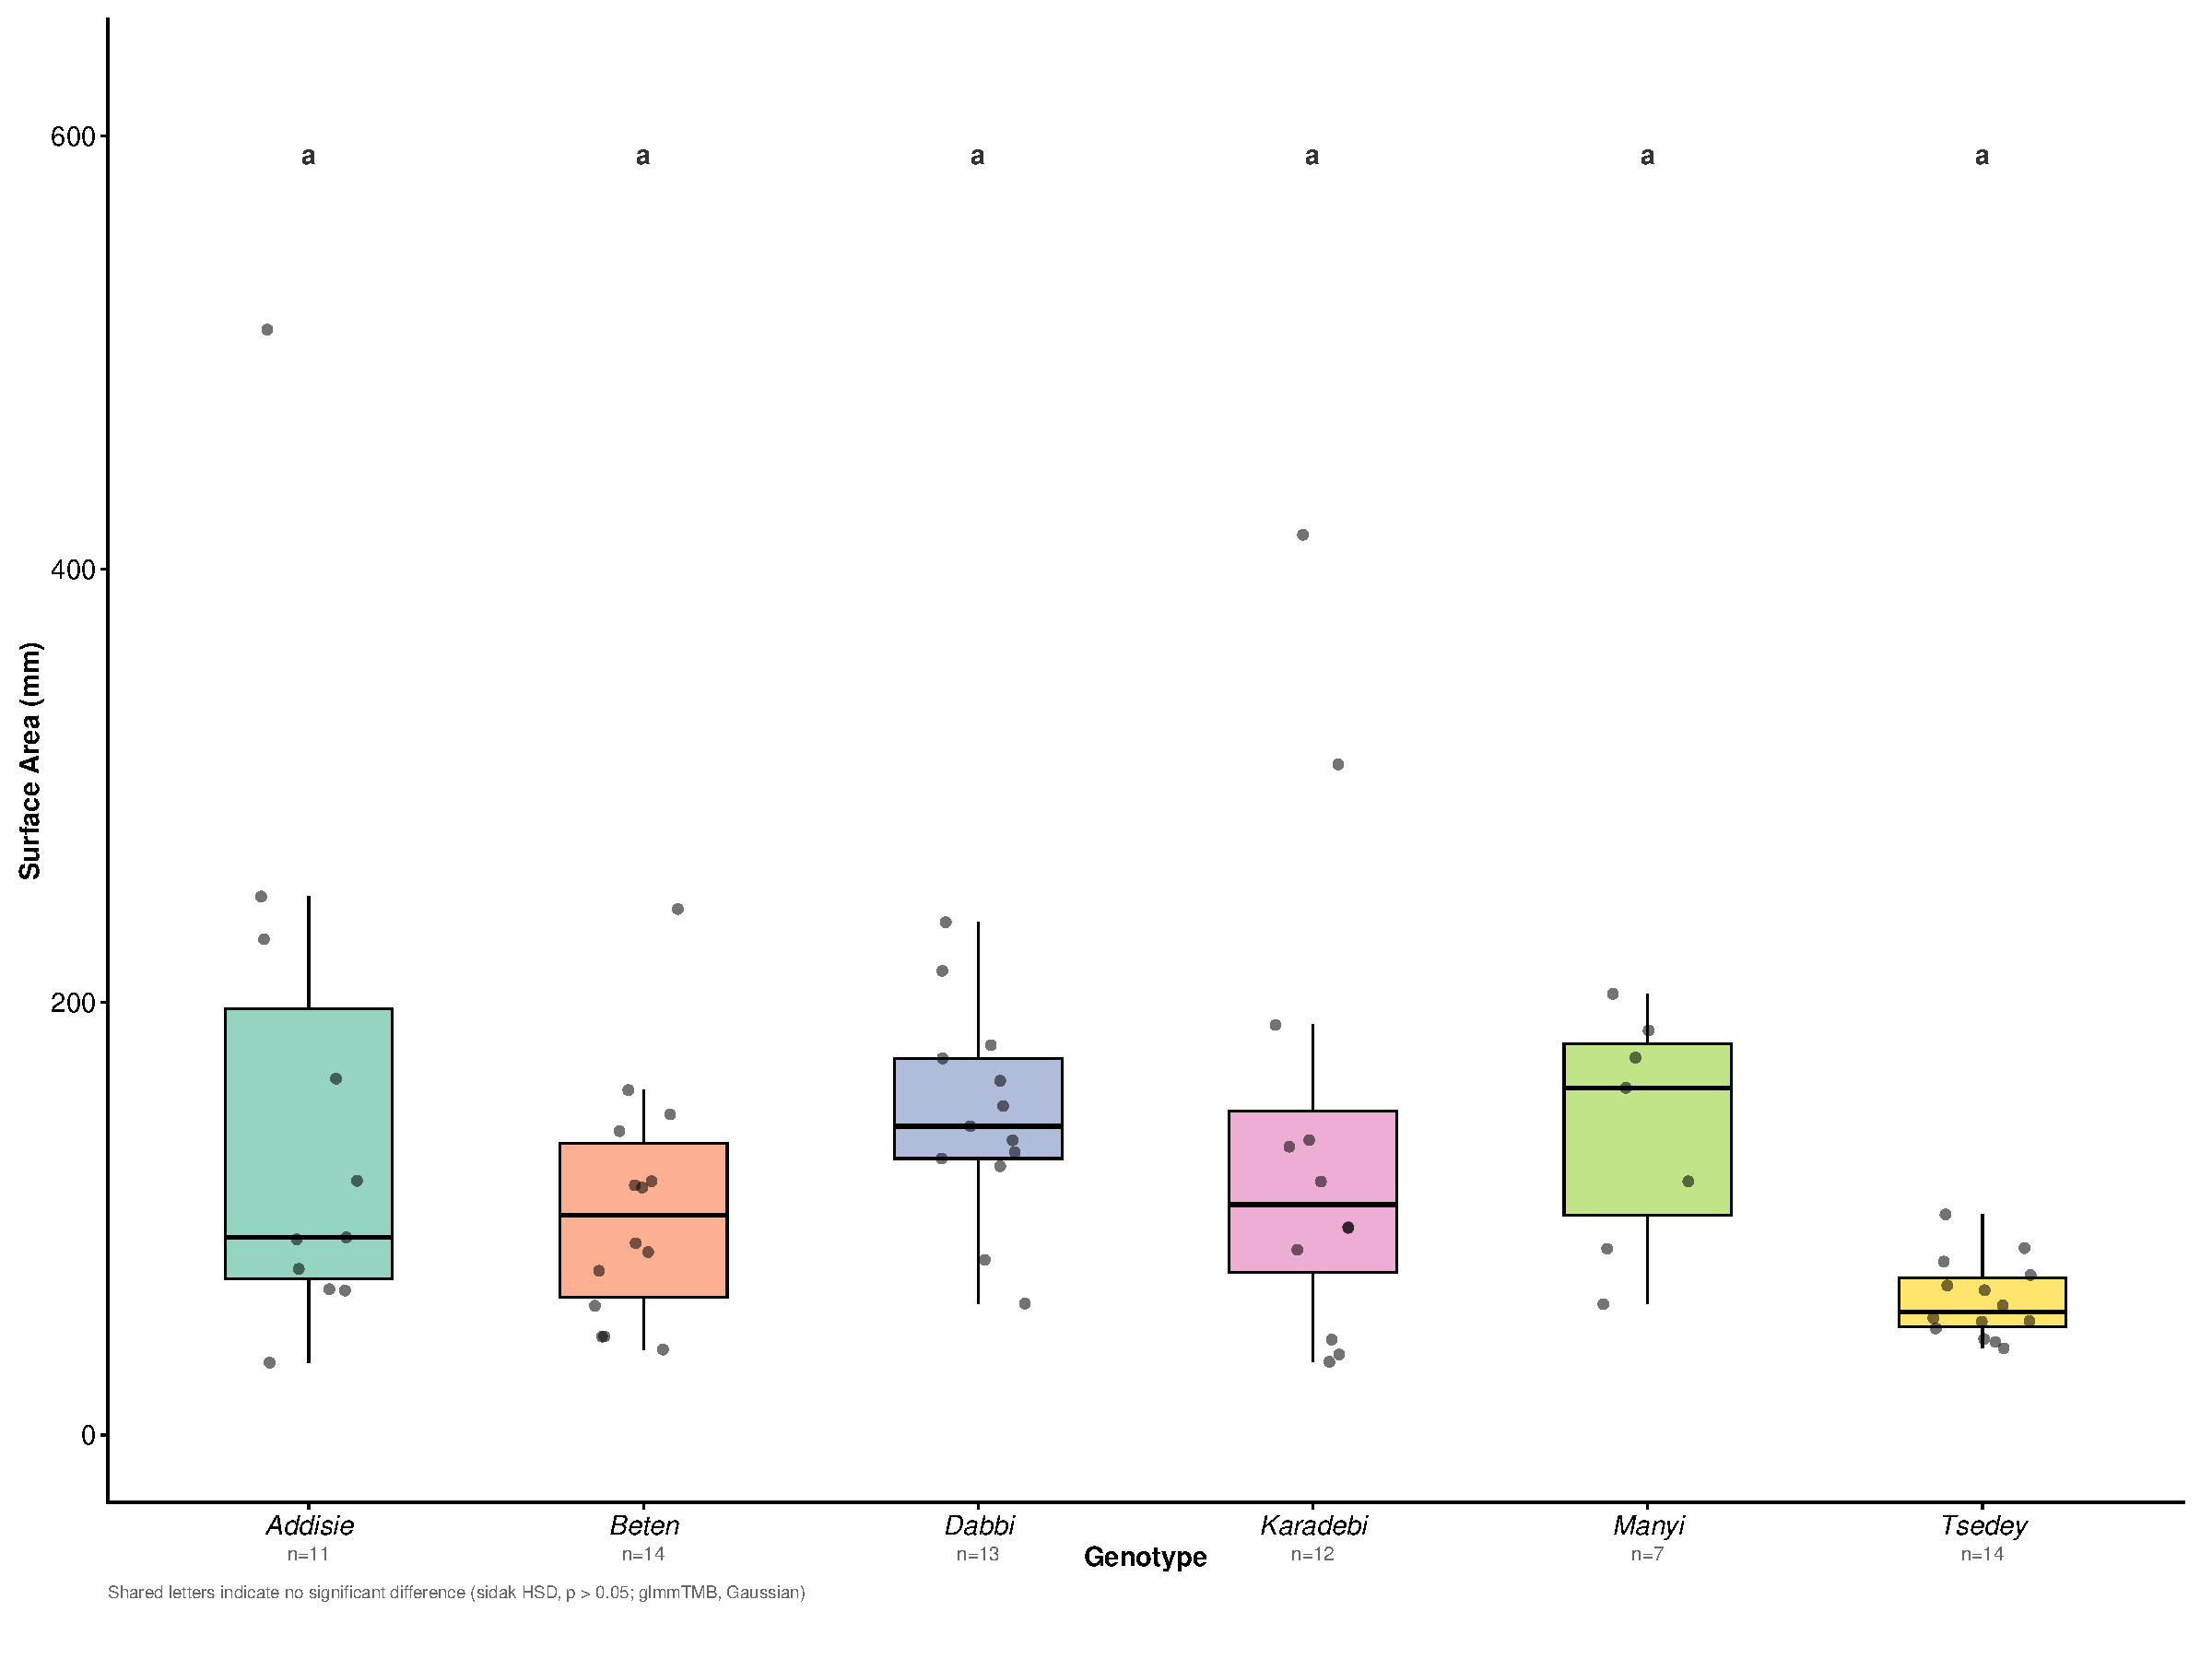
\includegraphics[keepaspectratio]{rsa_day1617_agar_files/figure-pdf/unnamed-chunk-11-6.pdf}}

\subsubsection{Volume}\label{volume}

\begin{Shaded}
\begin{Highlighting}[]
\CommentTok{\# ============================================================}
\CommentTok{\# Volume Analysis  }
\CommentTok{\# Positive continuous — start raw Gaussian, log if needed}
\CommentTok{\# ============================================================}

\CommentTok{\# Per{-}genotype Var/Mean — Poisson assumes Var = Mean exactly.}
\CommentTok{\# Ratios \textgreater{}\textgreater{} 1 within genotypes suggest NB is needed.}
\NormalTok{df }\SpecialCharTok{\%\textgreater{}\%}
  \FunctionTok{group\_by}\NormalTok{(Genotype) }\SpecialCharTok{\%\textgreater{}\%}
  \FunctionTok{summarise}\NormalTok{(}\AttributeTok{Mean     =} \FunctionTok{round}\NormalTok{(}\FunctionTok{mean}\NormalTok{(Volume.mm3), }\DecValTok{2}\NormalTok{),}
            \AttributeTok{Variance =} \FunctionTok{round}\NormalTok{(}\FunctionTok{var}\NormalTok{(Volume.mm3),  }\DecValTok{2}\NormalTok{),}
            \AttributeTok{Var\_Mean =} \FunctionTok{round}\NormalTok{(}\FunctionTok{var}\NormalTok{(Volume.mm3) }\SpecialCharTok{/}
                               \FunctionTok{mean}\NormalTok{(Volume.mm3), }\DecValTok{2}\NormalTok{))}
\end{Highlighting}
\end{Shaded}

\begin{verbatim}
# A tibble: 6 x 4
  Genotype  Mean Variance Var_Mean
  <fct>    <dbl>    <dbl>    <dbl>
1 Addisie  16.4    376.      22.8 
2 Beten     8.09    19.9      2.46
3 Dabbi    11.2     18.6      1.66
4 Karadebi 11.6    141.      12.2 
5 Manyi    15.4     38.4      2.5 
6 Tsedey    4.69     2.76     0.59
\end{verbatim}

\begin{Shaded}
\begin{Highlighting}[]
\CommentTok{\# ── 1. Inspect distribution ───────────────────────────────────}
\FunctionTok{summary}\NormalTok{(df}\SpecialCharTok{$}\NormalTok{Volume.mm3)}
\end{Highlighting}
\end{Shaded}

\begin{verbatim}
   Min. 1st Qu.  Median    Mean 3rd Qu.    Max. 
  2.386   4.523   7.534  10.581  11.958  67.568 
\end{verbatim}

\begin{Shaded}
\begin{Highlighting}[]
\FunctionTok{hist}\NormalTok{(df}\SpecialCharTok{$}\NormalTok{Volume.mm3, }\AttributeTok{breaks =} \DecValTok{15}\NormalTok{, }\AttributeTok{main =} \StringTok{"Volume (mm³)"}\NormalTok{)}
\end{Highlighting}
\end{Shaded}

\pandocbounded{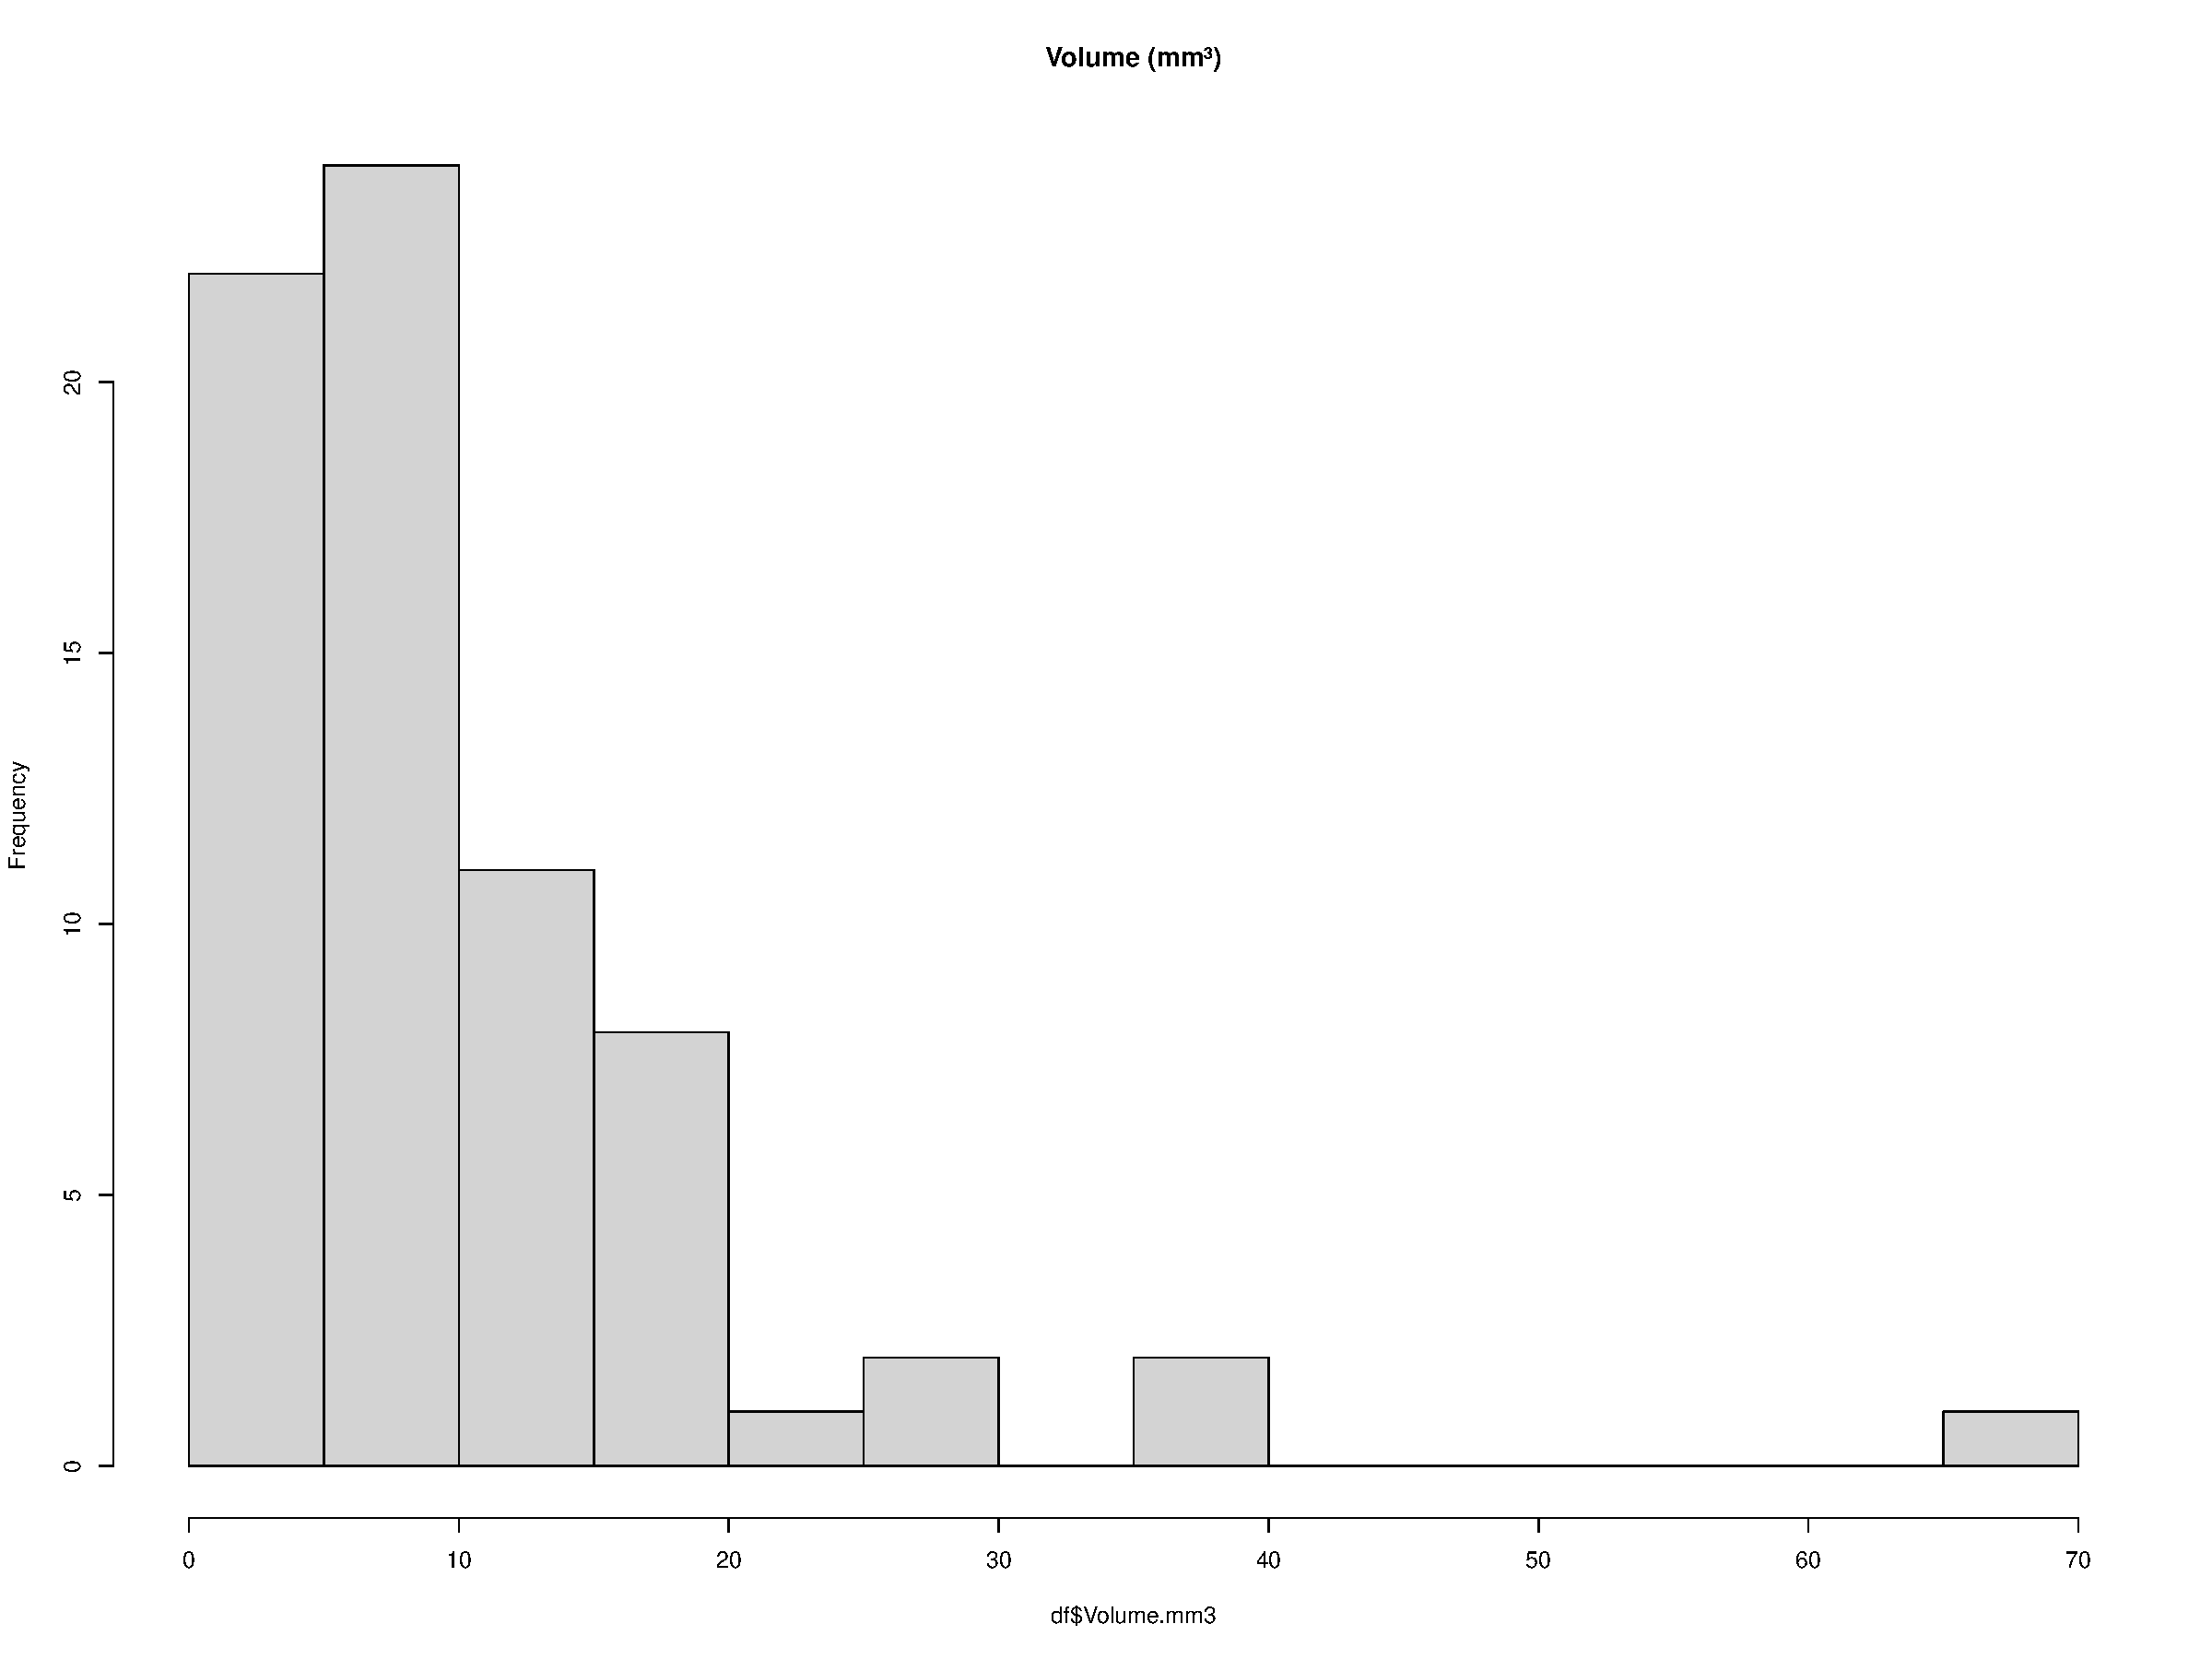
\includegraphics[keepaspectratio]{rsa_day1617_agar_files/figure-pdf/unnamed-chunk-12-1.pdf}}

\begin{Shaded}
\begin{Highlighting}[]
\CommentTok{\# ── 2. Fit models ────────────────────────────────────────}
\NormalTok{Vol\_raw }\OtherTok{\textless{}{-}} \FunctionTok{glmmTMB}\NormalTok{(}
\NormalTok{  Volume.mm3 }\SpecialCharTok{\textasciitilde{}}\NormalTok{ Genotype }\SpecialCharTok{+}\NormalTok{ (}\DecValTok{1} \SpecialCharTok{|}\NormalTok{ Batch}\SpecialCharTok{/}\NormalTok{Plate}\SpecialCharTok{/}\NormalTok{Seed),}
  \AttributeTok{data =}\NormalTok{ df, }
  \AttributeTok{family =} \FunctionTok{gaussian}\NormalTok{()}
\NormalTok{)}

\FunctionTok{VarCorr}\NormalTok{(Vol\_raw)}
\end{Highlighting}
\end{Shaded}

\begin{verbatim}

Conditional model:
 Groups           Name        Std.Dev.
 Seed:Plate:Batch (Intercept) 0.026298
 Plate:Batch      (Intercept) 1.986217
 Batch            (Intercept) 3.992394
 Residual                     8.237707
\end{verbatim}

\begin{Shaded}
\begin{Highlighting}[]
\FunctionTok{check\_singularity}\NormalTok{(Vol\_raw)}
\end{Highlighting}
\end{Shaded}

\begin{verbatim}
[1] FALSE
\end{verbatim}

\begin{Shaded}
\begin{Highlighting}[]
\FunctionTok{summary}\NormalTok{(Vol\_raw)}
\end{Highlighting}
\end{Shaded}

\begin{verbatim}
 Family: gaussian  ( identity )
Formula:          Volume.mm3 ~ Genotype + (1 | Batch/Plate/Seed)
Data: df

      AIC       BIC    logLik -2*log(L)  df.resid 
    530.2     552.8    -255.1     510.2        61 

Random effects:

Conditional model:
 Groups           Name        Variance  Std.Dev.
 Seed:Plate:Batch (Intercept) 6.916e-04 0.0263  
 Plate:Batch      (Intercept) 3.945e+00 1.9862  
 Batch            (Intercept) 1.594e+01 3.9924  
 Residual                     6.786e+01 8.2377  
Number of obs: 71, groups:  Seed:Plate:Batch, 38; Plate:Batch, 18; Batch, 4

Dispersion estimate for gaussian family (sigma^2): 67.9 

Conditional model:
                 Estimate Std. Error z value Pr(>|z|)    
(Intercept)        17.114      3.455   4.953 7.31e-07 ***
GenotypeBeten      -7.432      3.493  -2.127  0.03338 *  
GenotypeDabbi     -10.048      4.129  -2.433  0.01497 *  
GenotypeKaradebi   -5.801      3.868  -1.500  0.13364    
GenotypeManyi      -2.201      4.531  -0.486  0.62707    
GenotypeTsedey    -11.014      3.740  -2.945  0.00323 ** 
---
Signif. codes:  0 '***' 0.001 '**' 0.01 '*' 0.05 '.' 0.1 ' ' 1
\end{verbatim}

\begin{Shaded}
\begin{Highlighting}[]
\CommentTok{\# ── 4. Diagnostics: raw model ────────────────────────────────}
\NormalTok{sim\_res\_raw }\OtherTok{\textless{}{-}} \FunctionTok{simulateResiduals}\NormalTok{(Vol\_raw, }\AttributeTok{n =} \DecValTok{1000}\NormalTok{)}
\FunctionTok{plot}\NormalTok{(sim\_res\_raw)}
\end{Highlighting}
\end{Shaded}

\pandocbounded{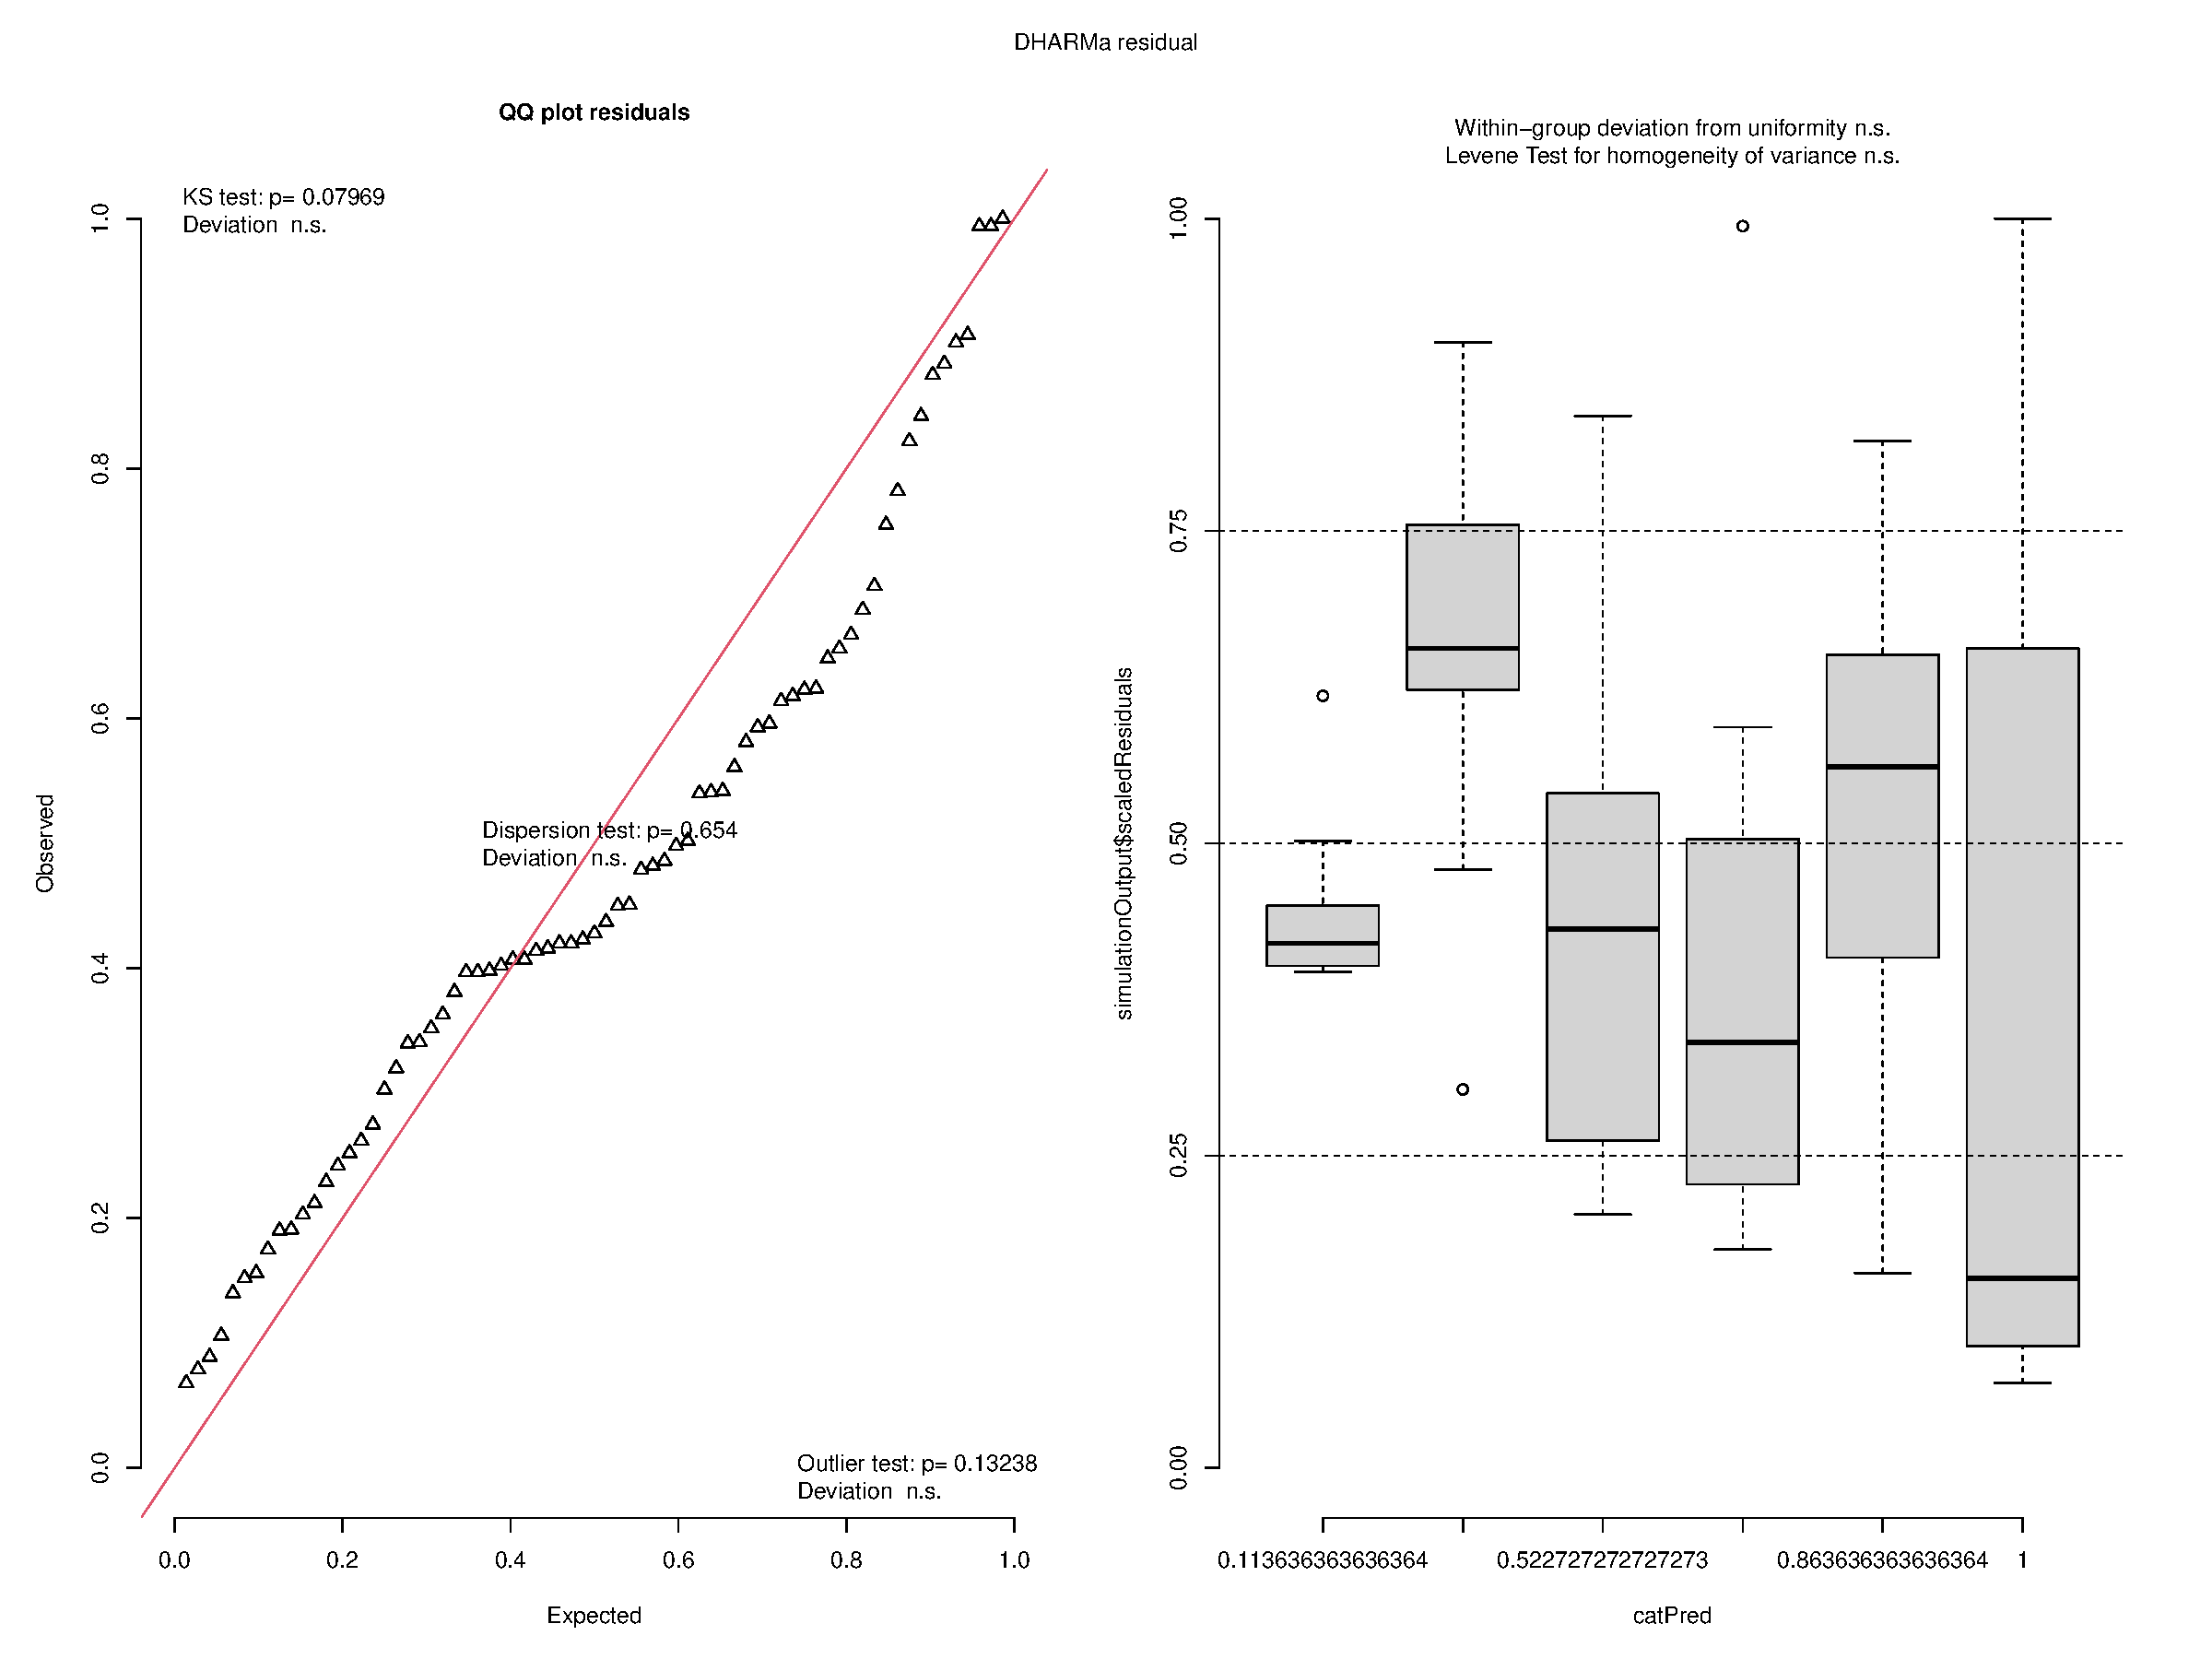
\includegraphics[keepaspectratio]{rsa_day1617_agar_files/figure-pdf/unnamed-chunk-12-2.pdf}}

\begin{Shaded}
\begin{Highlighting}[]
\FunctionTok{testUniformity}\NormalTok{(sim\_res\_raw)    }\CommentTok{\# p \textgreater{} 0.05 = good}
\end{Highlighting}
\end{Shaded}

\pandocbounded{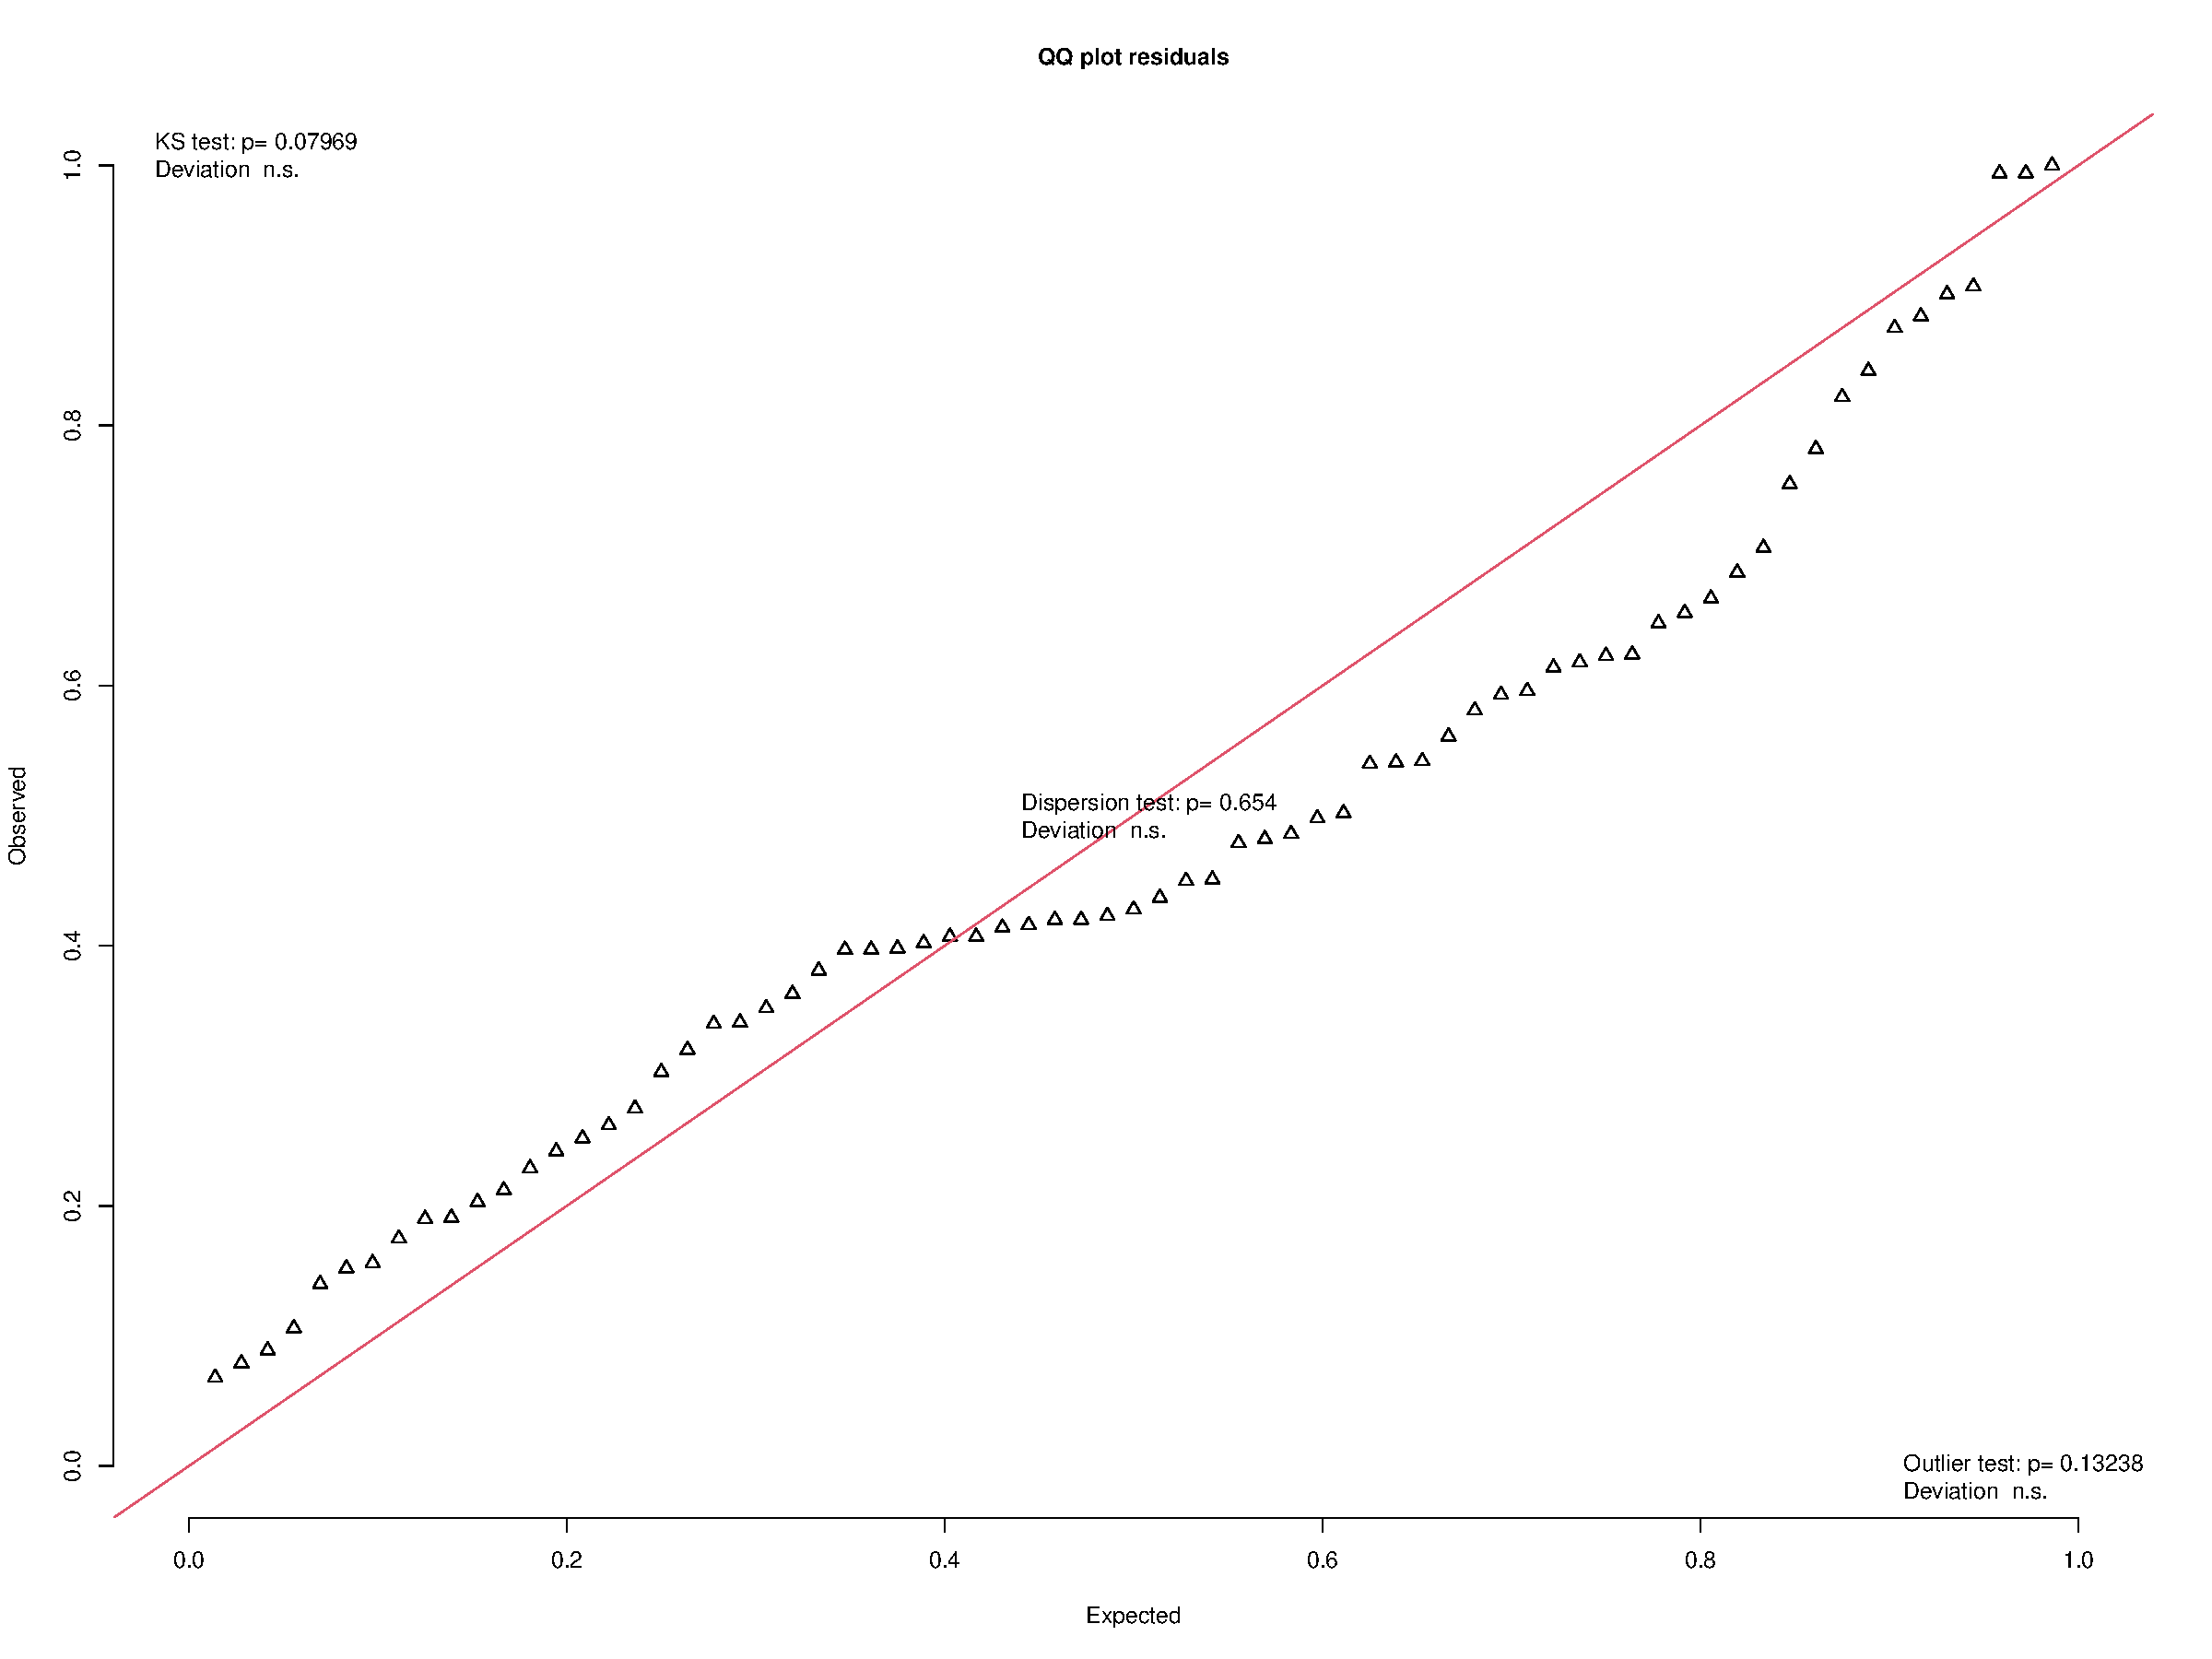
\includegraphics[keepaspectratio]{rsa_day1617_agar_files/figure-pdf/unnamed-chunk-12-3.pdf}}

\begin{verbatim}

    Asymptotic one-sample Kolmogorov-Smirnov test

data:  simulationOutput$scaledResiduals
D = 0.15065, p-value = 0.07969
alternative hypothesis: two-sided
\end{verbatim}

\begin{Shaded}
\begin{Highlighting}[]
\FunctionTok{testDispersion}\NormalTok{(sim\_res\_raw)    }\CommentTok{\# ratio ≈ 1.0}
\end{Highlighting}
\end{Shaded}

\pandocbounded{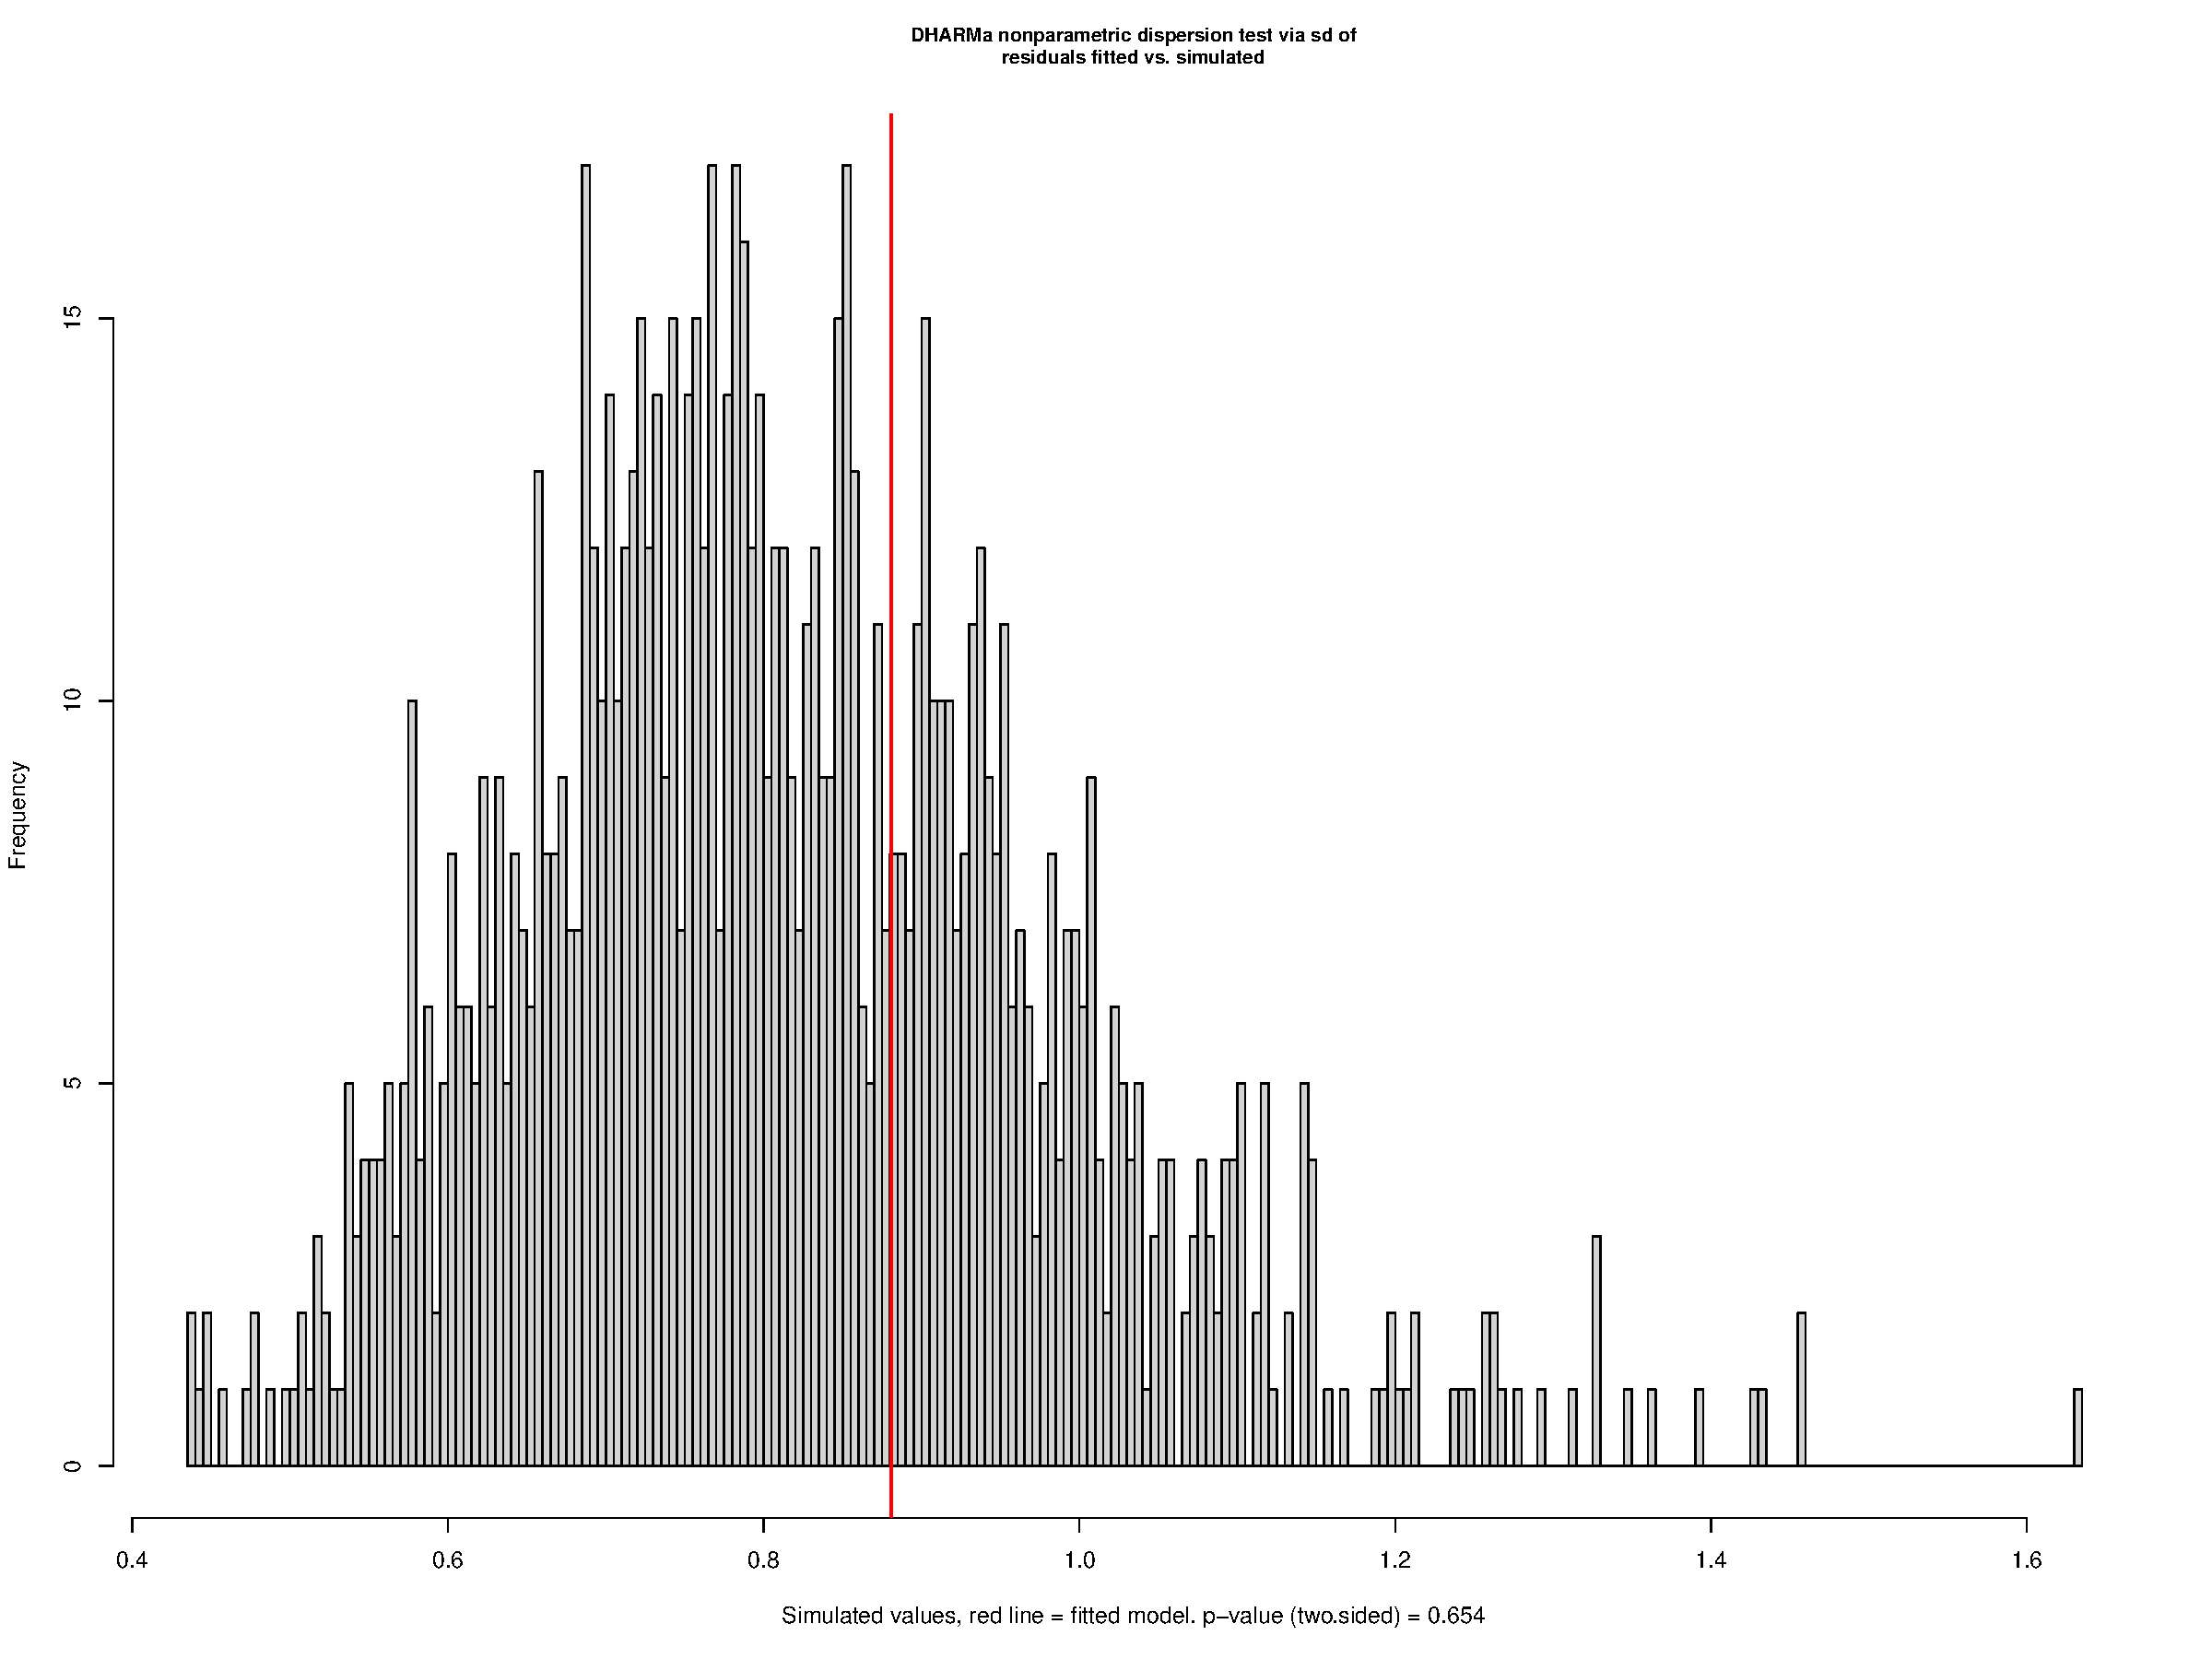
\includegraphics[keepaspectratio]{rsa_day1617_agar_files/figure-pdf/unnamed-chunk-12-4.pdf}}

\begin{verbatim}

    DHARMa nonparametric dispersion test via sd of residuals fitted vs.
    simulated

data:  simulationOutput
dispersion = 1.0777, p-value = 0.654
alternative hypothesis: two.sided
\end{verbatim}

\begin{Shaded}
\begin{Highlighting}[]
\FunctionTok{plotResiduals}\NormalTok{(sim\_res\_raw, }\AttributeTok{form =}\NormalTok{ df}\SpecialCharTok{$}\NormalTok{Genotype)}
\end{Highlighting}
\end{Shaded}

\pandocbounded{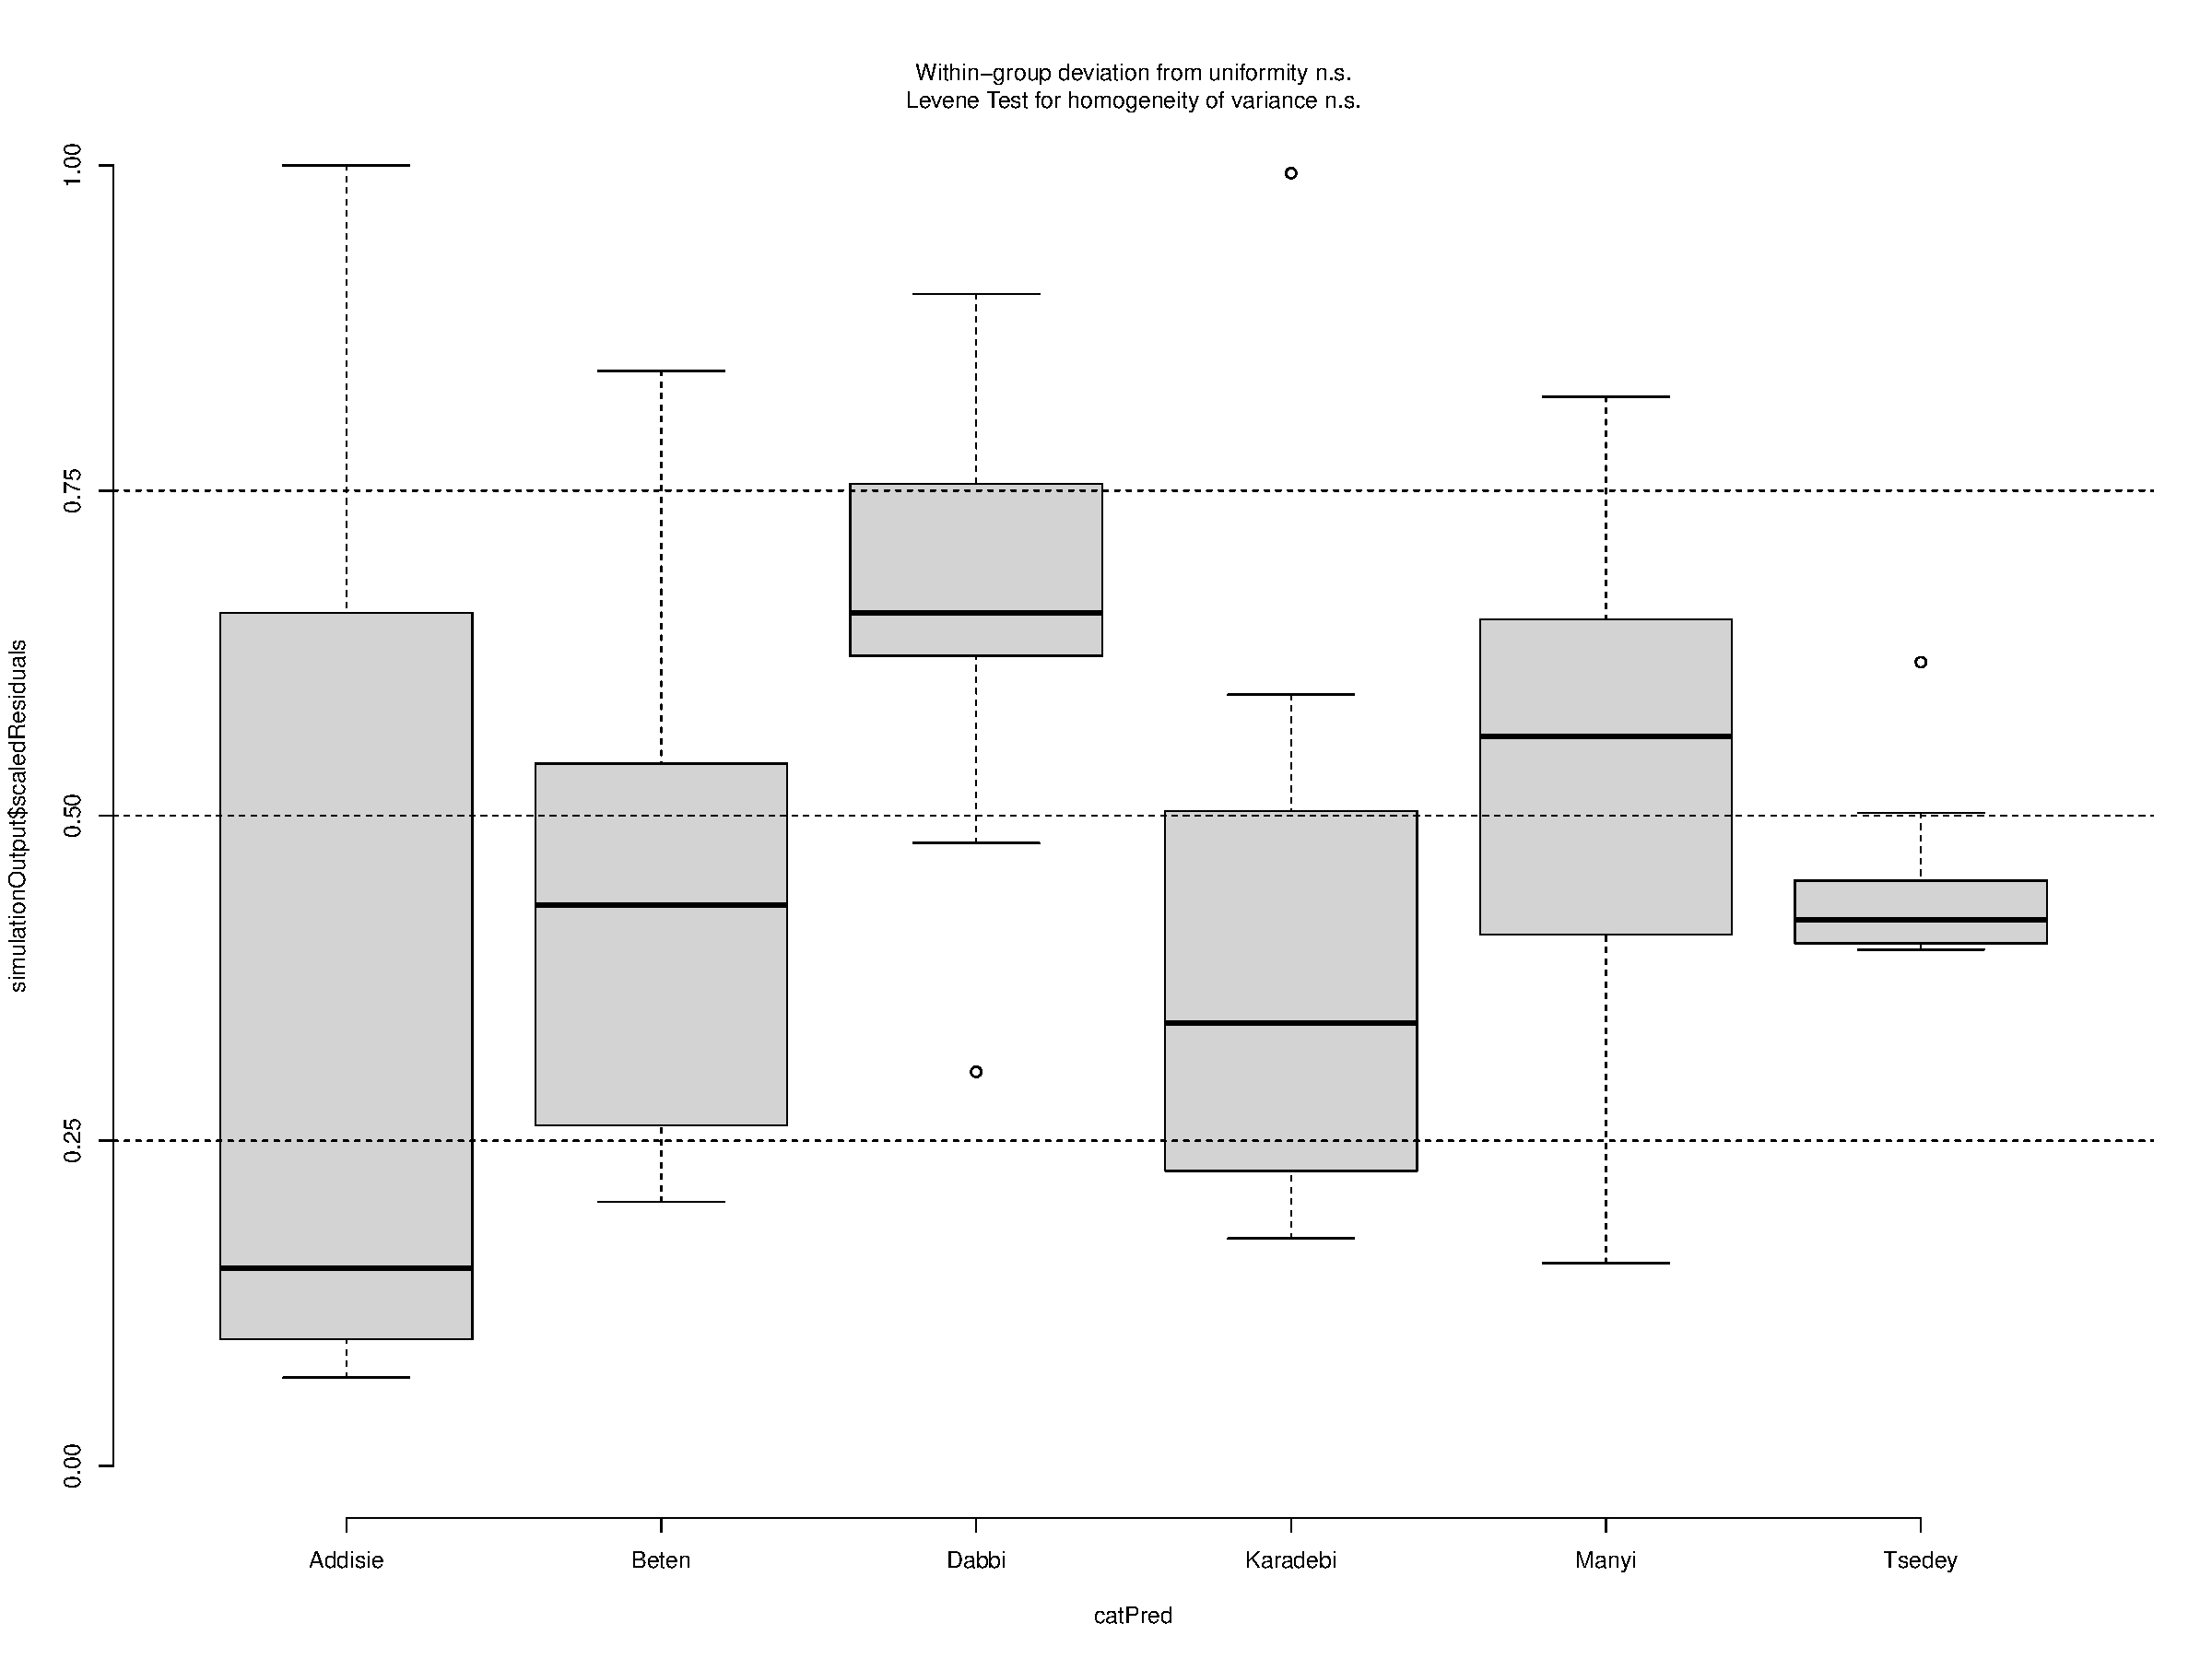
\includegraphics[keepaspectratio]{rsa_day1617_agar_files/figure-pdf/unnamed-chunk-12-5.pdf}}

\begin{Shaded}
\begin{Highlighting}[]
\CommentTok{\# some snaking so will try log transforming to see if there is an improved fit}
\NormalTok{Vol\_raw }\OtherTok{\textless{}{-}} \FunctionTok{glmmTMB}\NormalTok{(}
  \FunctionTok{log}\NormalTok{(Volume.mm3) }\SpecialCharTok{\textasciitilde{}}\NormalTok{ Genotype }\SpecialCharTok{+}\NormalTok{ (}\DecValTok{1} \SpecialCharTok{|}\NormalTok{ Batch}\SpecialCharTok{/}\NormalTok{Plate}\SpecialCharTok{/}\NormalTok{Seed),}
  \AttributeTok{data =}\NormalTok{ df, }
  \AttributeTok{family =} \FunctionTok{gaussian}\NormalTok{()}
\NormalTok{)}

\FunctionTok{VarCorr}\NormalTok{(Vol\_raw)}
\end{Highlighting}
\end{Shaded}

\begin{verbatim}

Conditional model:
 Groups           Name        Std.Dev.  
 Seed:Plate:Batch (Intercept) 1.5911e-05
 Plate:Batch      (Intercept) 1.4074e-01
 Batch            (Intercept) 3.4124e-01
 Residual                     5.2779e-01
\end{verbatim}

\begin{Shaded}
\begin{Highlighting}[]
\FunctionTok{summary}\NormalTok{(Vol\_raw)}
\end{Highlighting}
\end{Shaded}

\begin{verbatim}
 Family: gaussian  ( identity )
Formula:          log(Volume.mm3) ~ Genotype + (1 | Batch/Plate/Seed)
Data: df

      AIC       BIC    logLik -2*log(L)  df.resid 
    142.3     165.0     -61.2     122.3        61 

Random effects:

Conditional model:
 Groups           Name        Variance  Std.Dev. 
 Seed:Plate:Batch (Intercept) 2.532e-10 1.591e-05
 Plate:Batch      (Intercept) 1.981e-02 1.407e-01
 Batch            (Intercept) 1.164e-01 3.412e-01
 Residual                     2.786e-01 5.278e-01
Number of obs: 71, groups:  Seed:Plate:Batch, 38; Plate:Batch, 18; Batch, 4

Dispersion estimate for gaussian family (sigma^2): 0.279 

Conditional model:
                 Estimate Std. Error z value Pr(>|z|)    
(Intercept)        2.3551     0.2499   9.423  < 2e-16 ***
GenotypeBeten     -0.2895     0.2219  -1.305  0.19196    
GenotypeDabbi     -0.3775     0.2597  -1.454  0.14605    
GenotypeKaradebi  -0.2995     0.2485  -1.205  0.22804    
GenotypeManyi      0.2905     0.2916   0.996  0.31915    
GenotypeTsedey    -0.6809     0.2403  -2.833  0.00461 ** 
---
Signif. codes:  0 '***' 0.001 '**' 0.01 '*' 0.05 '.' 0.1 ' ' 1
\end{verbatim}

\begin{Shaded}
\begin{Highlighting}[]
\FunctionTok{check\_singularity}\NormalTok{(Vol\_raw)}
\end{Highlighting}
\end{Shaded}

\begin{verbatim}
[1] TRUE
\end{verbatim}

\begin{Shaded}
\begin{Highlighting}[]
\NormalTok{sim\_res\_raw }\OtherTok{\textless{}{-}} \FunctionTok{simulateResiduals}\NormalTok{(Vol\_raw, }\AttributeTok{n =} \DecValTok{1000}\NormalTok{)}
\FunctionTok{plot}\NormalTok{(sim\_res\_raw)}
\end{Highlighting}
\end{Shaded}

\pandocbounded{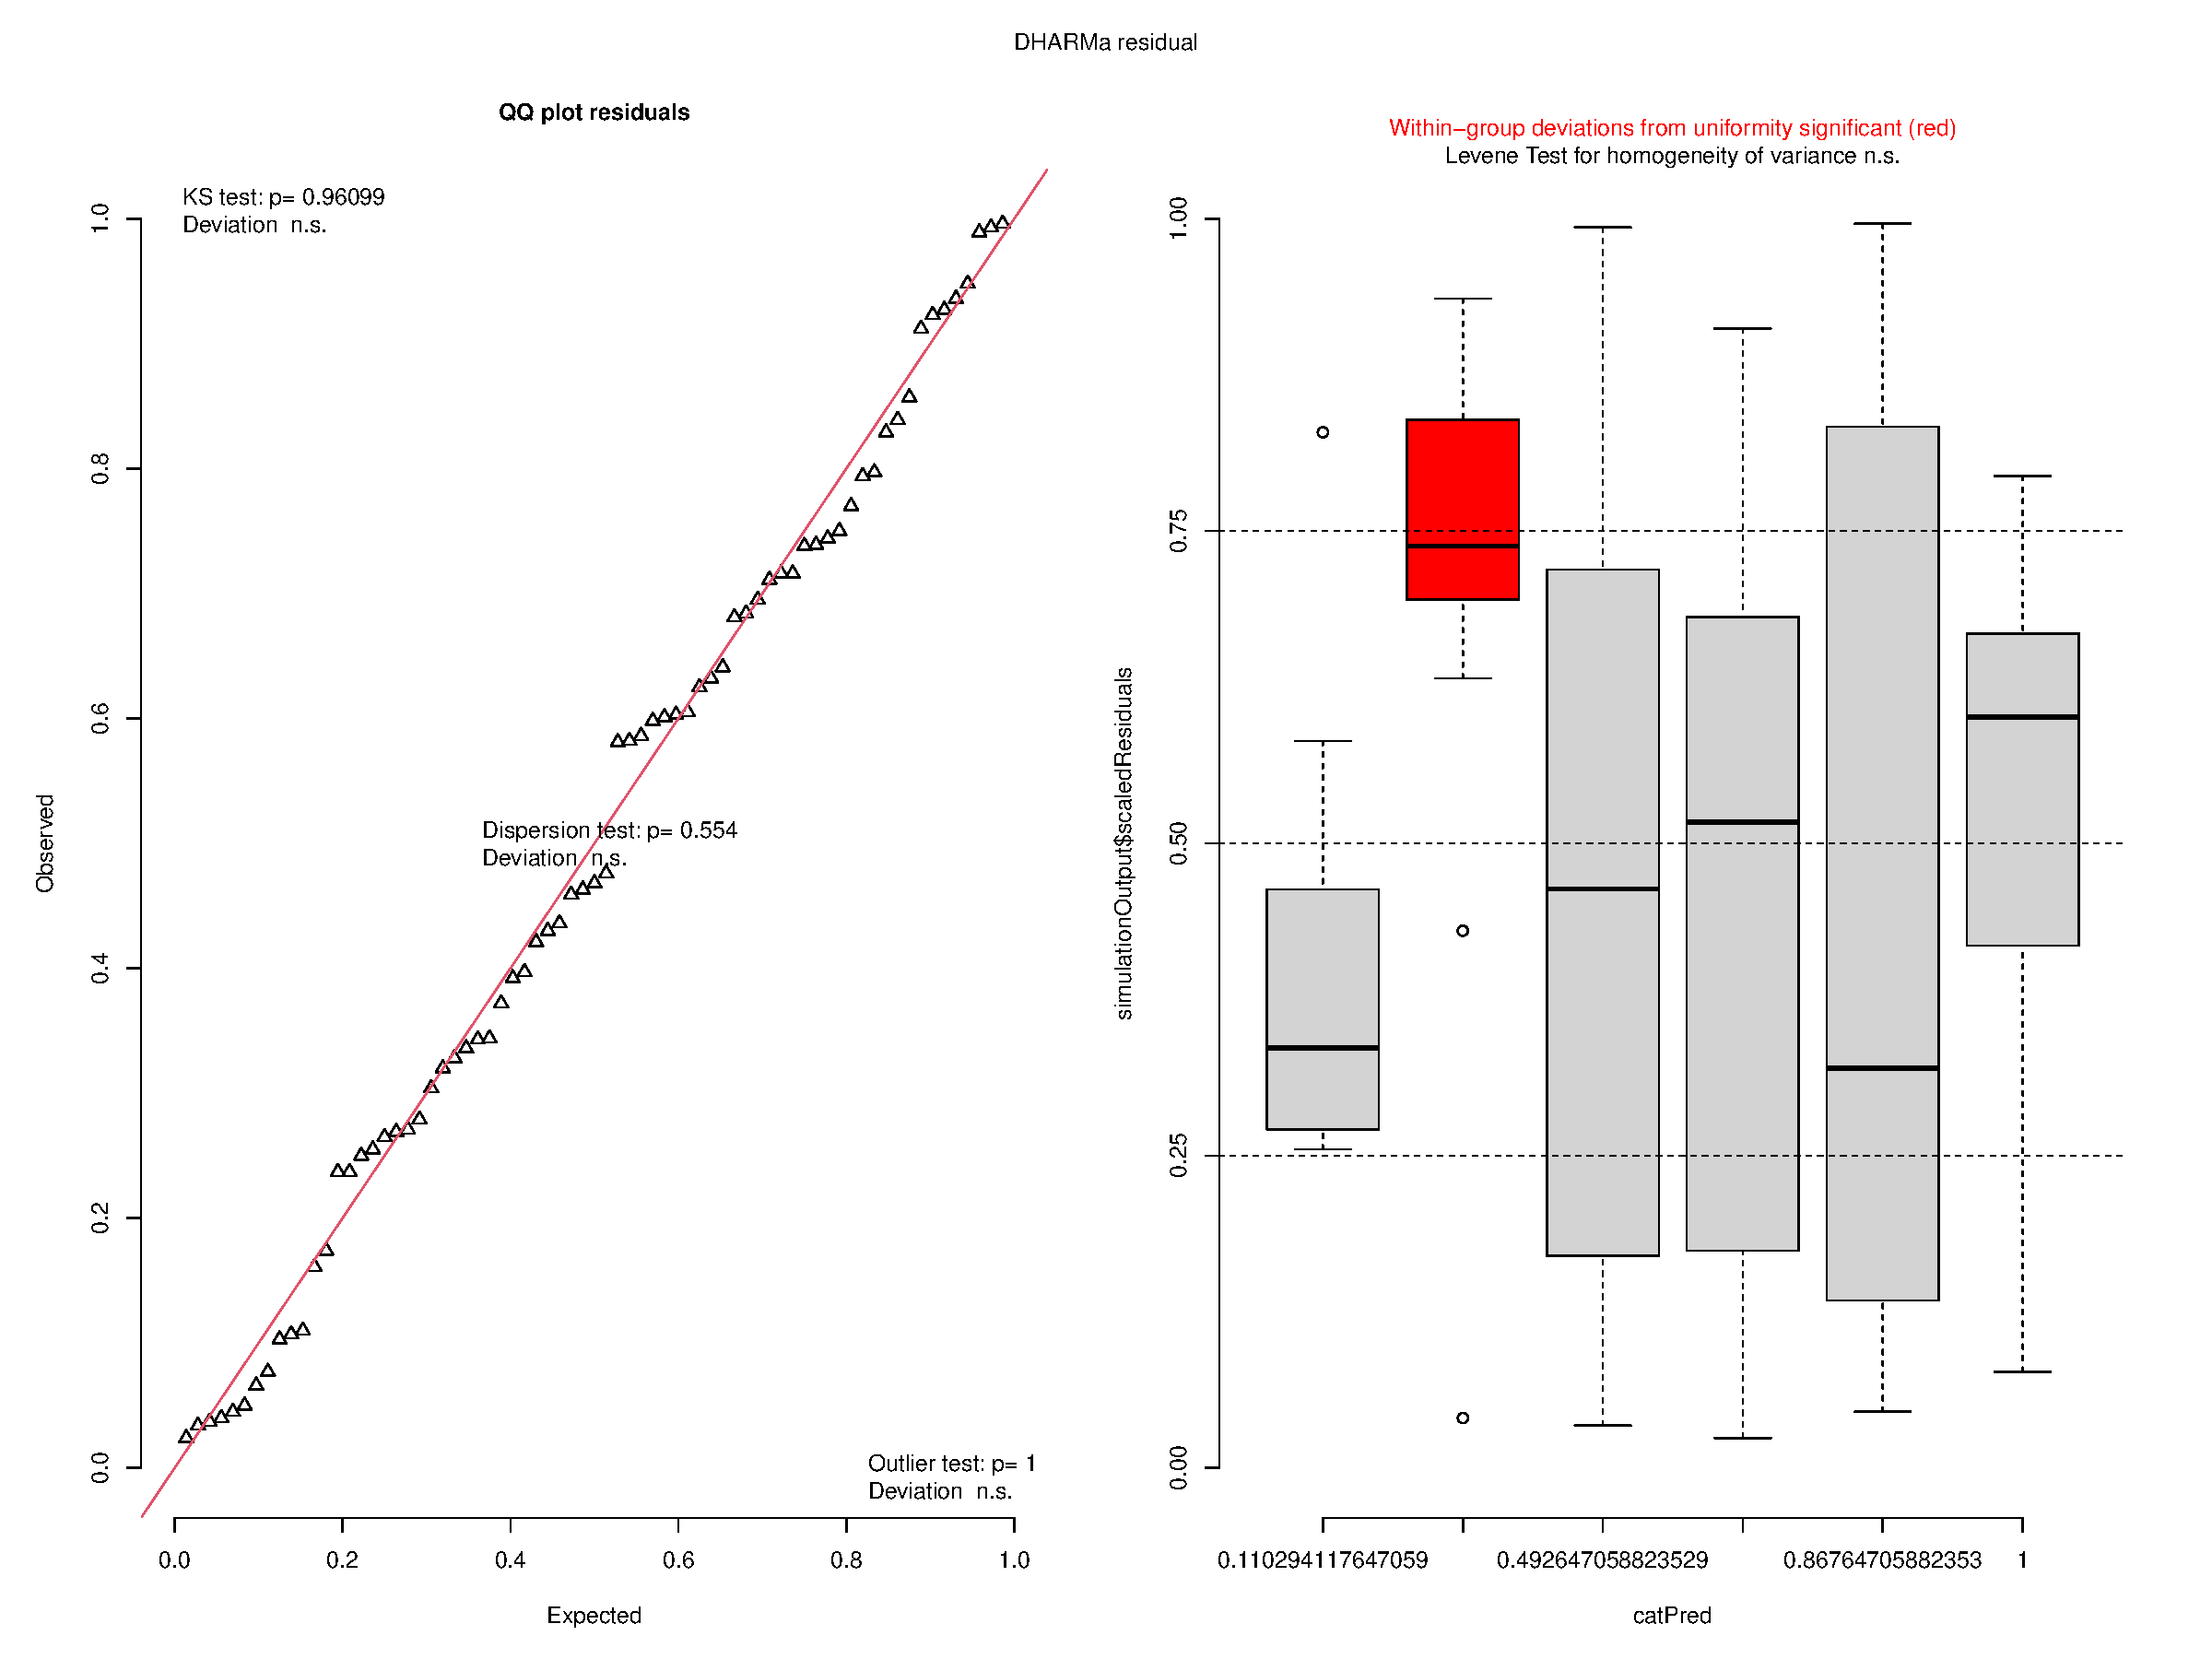
\includegraphics[keepaspectratio]{rsa_day1617_agar_files/figure-pdf/unnamed-chunk-12-6.pdf}}

\begin{Shaded}
\begin{Highlighting}[]
\FunctionTok{testUniformity}\NormalTok{(sim\_res\_raw)    }\CommentTok{\# p \textgreater{} 0.05 = good}
\end{Highlighting}
\end{Shaded}

\pandocbounded{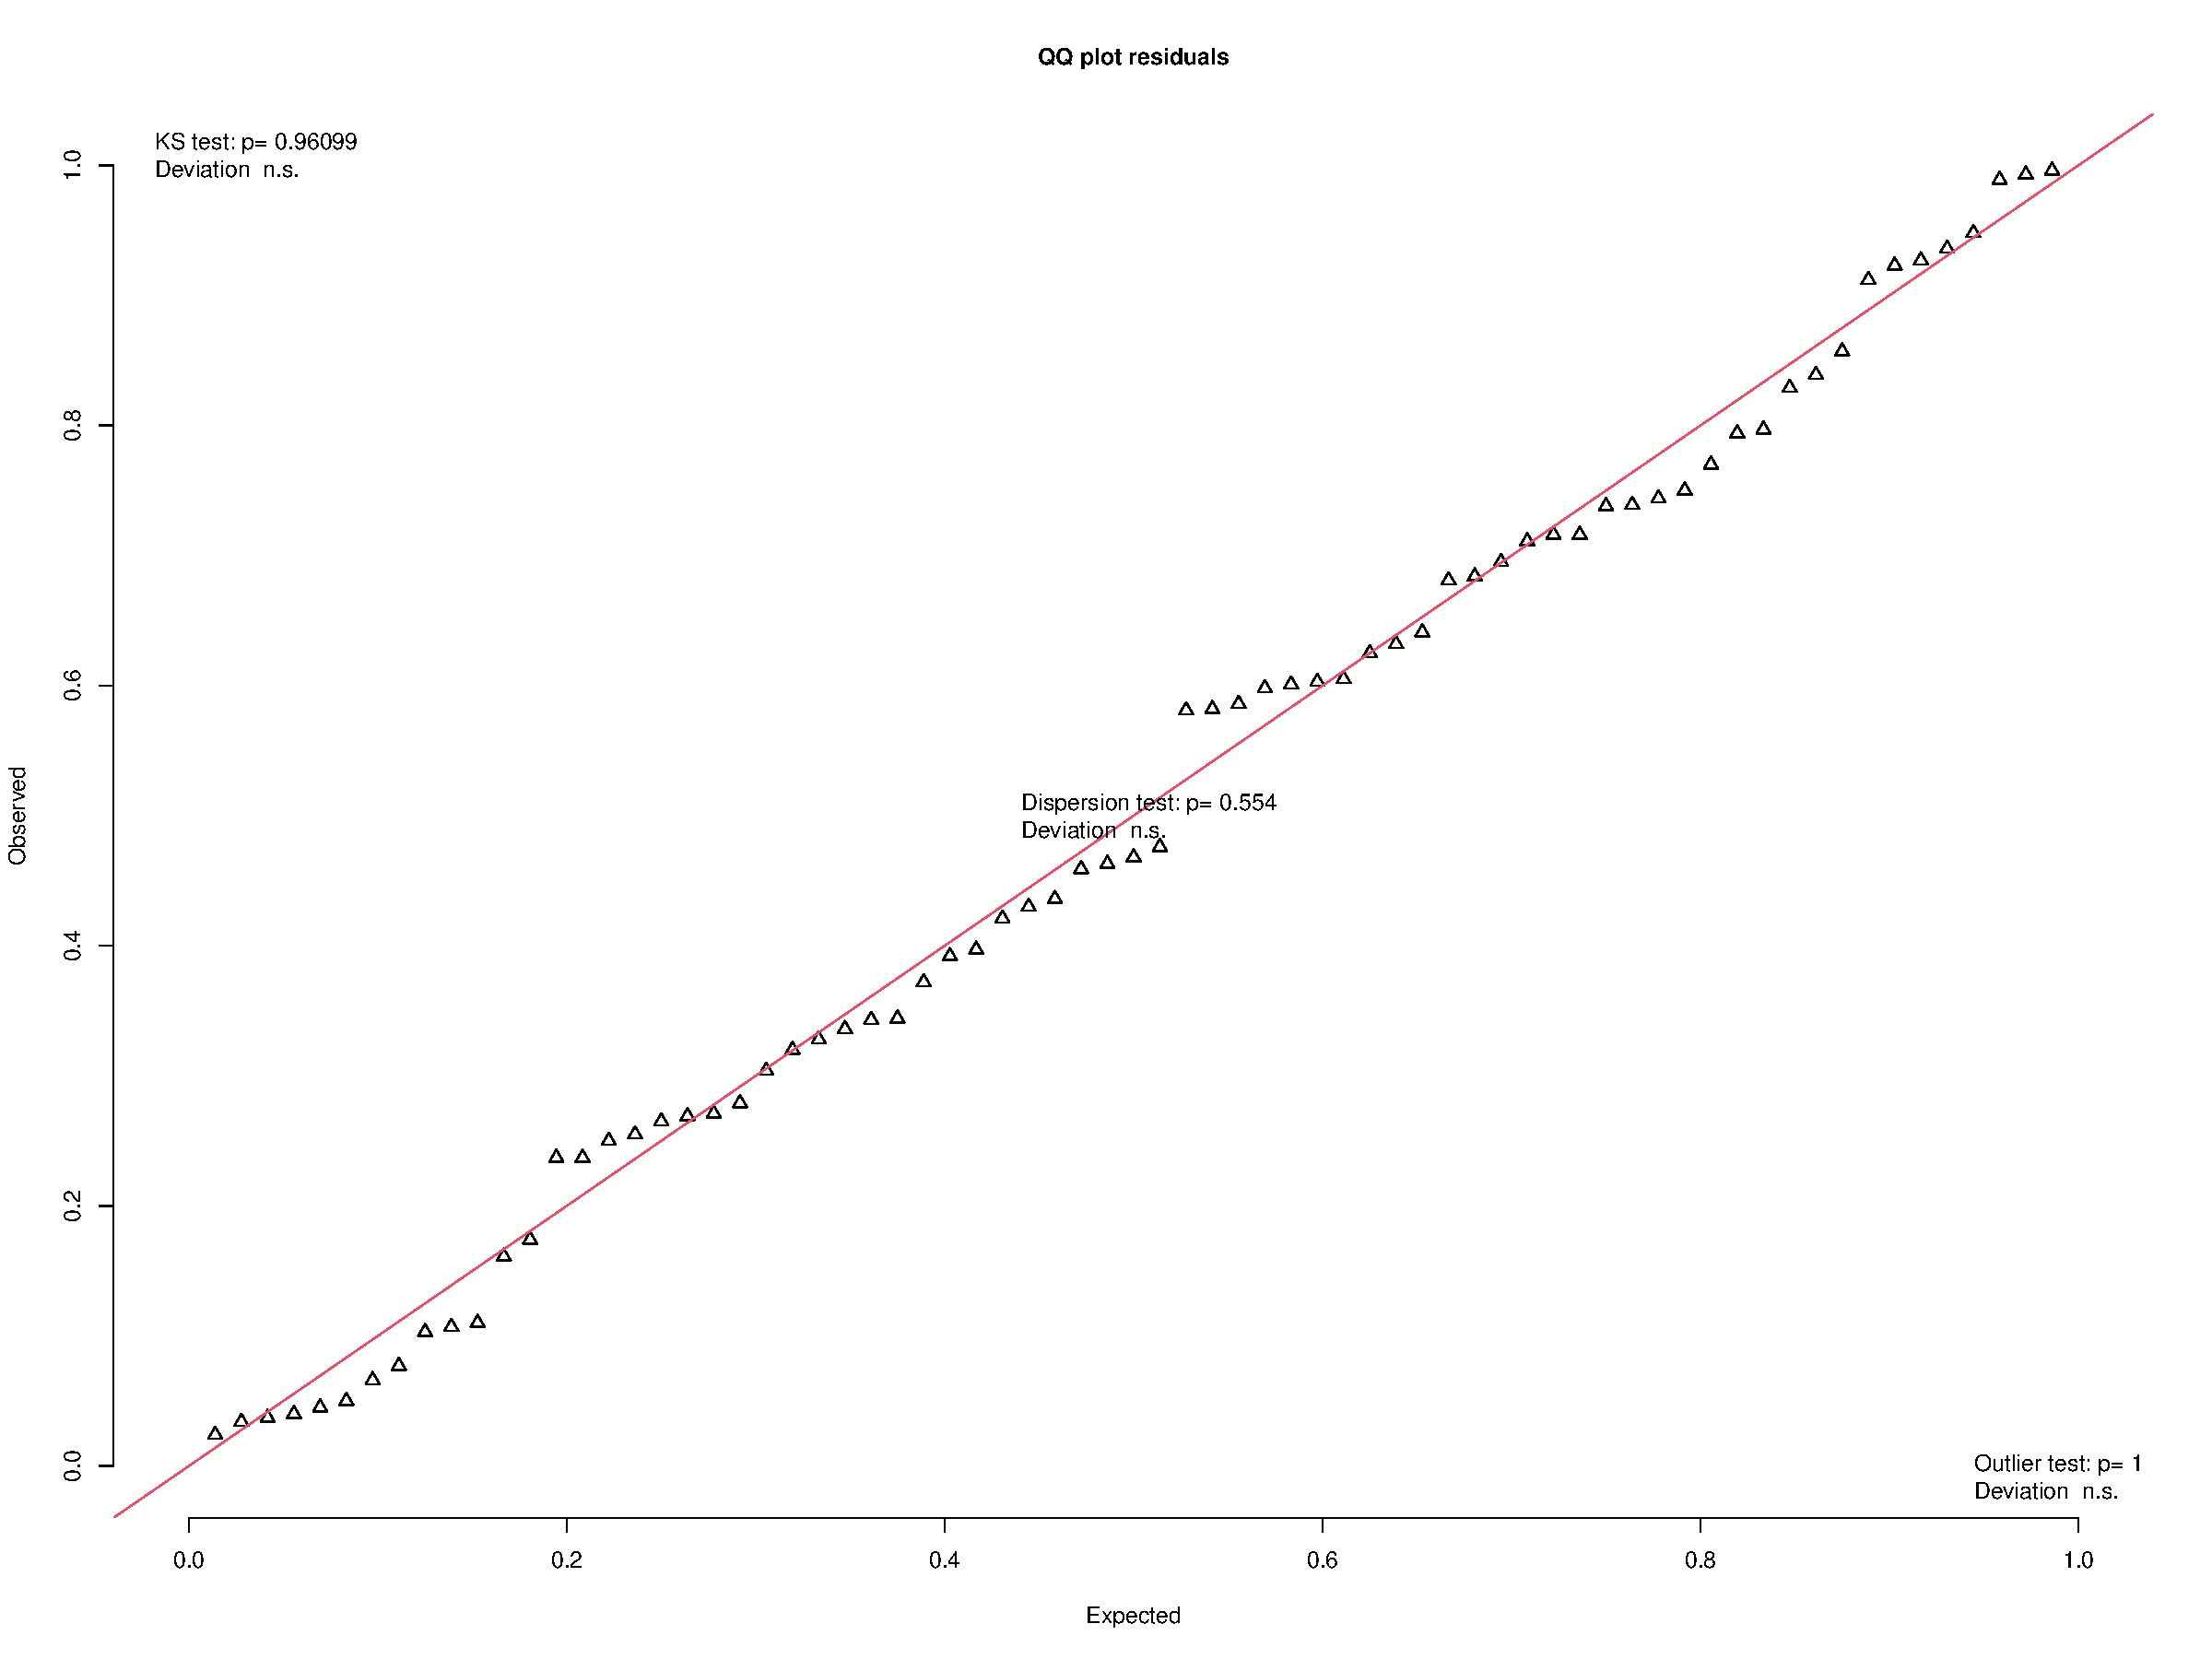
\includegraphics[keepaspectratio]{rsa_day1617_agar_files/figure-pdf/unnamed-chunk-12-7.pdf}}

\begin{verbatim}

    Asymptotic one-sample Kolmogorov-Smirnov test

data:  simulationOutput$scaledResiduals
D = 0.059873, p-value = 0.961
alternative hypothesis: two-sided
\end{verbatim}

\begin{Shaded}
\begin{Highlighting}[]
\FunctionTok{testDispersion}\NormalTok{(sim\_res\_raw)    }\CommentTok{\# ratio ≈ 1.0}
\end{Highlighting}
\end{Shaded}

\pandocbounded{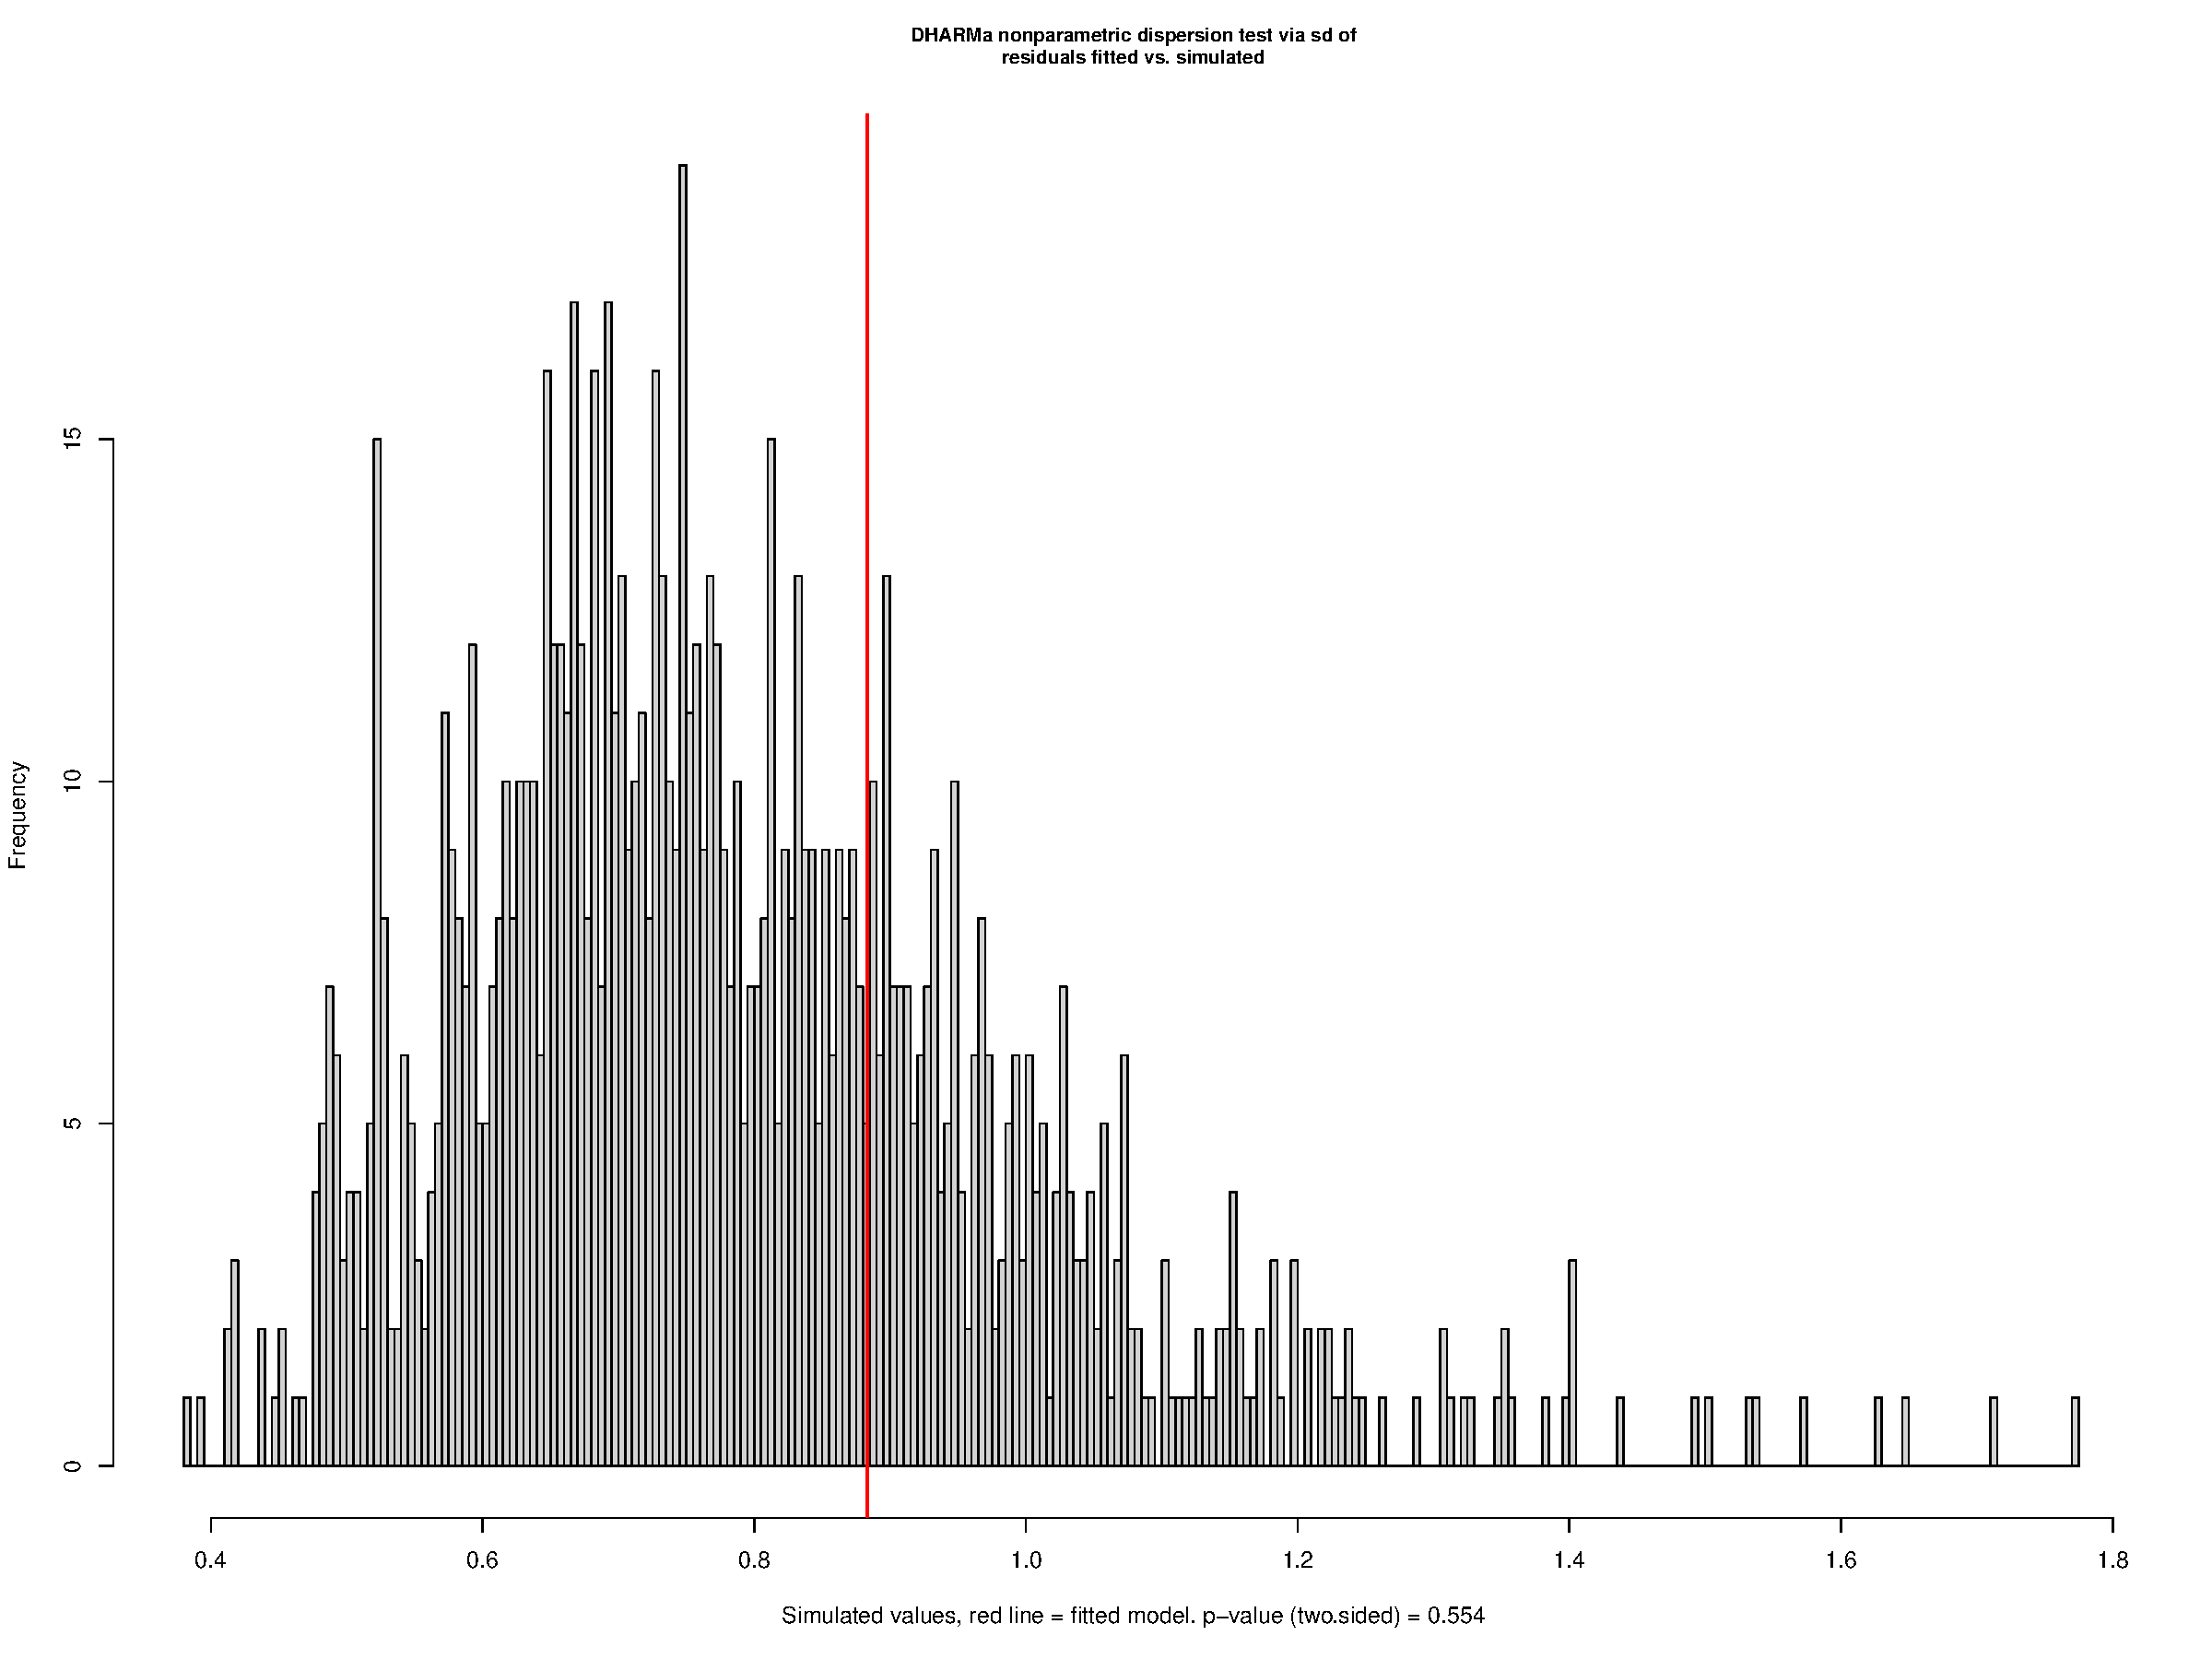
\includegraphics[keepaspectratio]{rsa_day1617_agar_files/figure-pdf/unnamed-chunk-12-8.pdf}}

\begin{verbatim}

    DHARMa nonparametric dispersion test via sd of residuals fitted vs.
    simulated

data:  simulationOutput
dispersion = 1.1202, p-value = 0.554
alternative hypothesis: two.sided
\end{verbatim}

\begin{Shaded}
\begin{Highlighting}[]
\FunctionTok{plotResiduals}\NormalTok{(sim\_res\_raw, }\AttributeTok{form =}\NormalTok{ df}\SpecialCharTok{$}\NormalTok{Genotype)}
\end{Highlighting}
\end{Shaded}

\pandocbounded{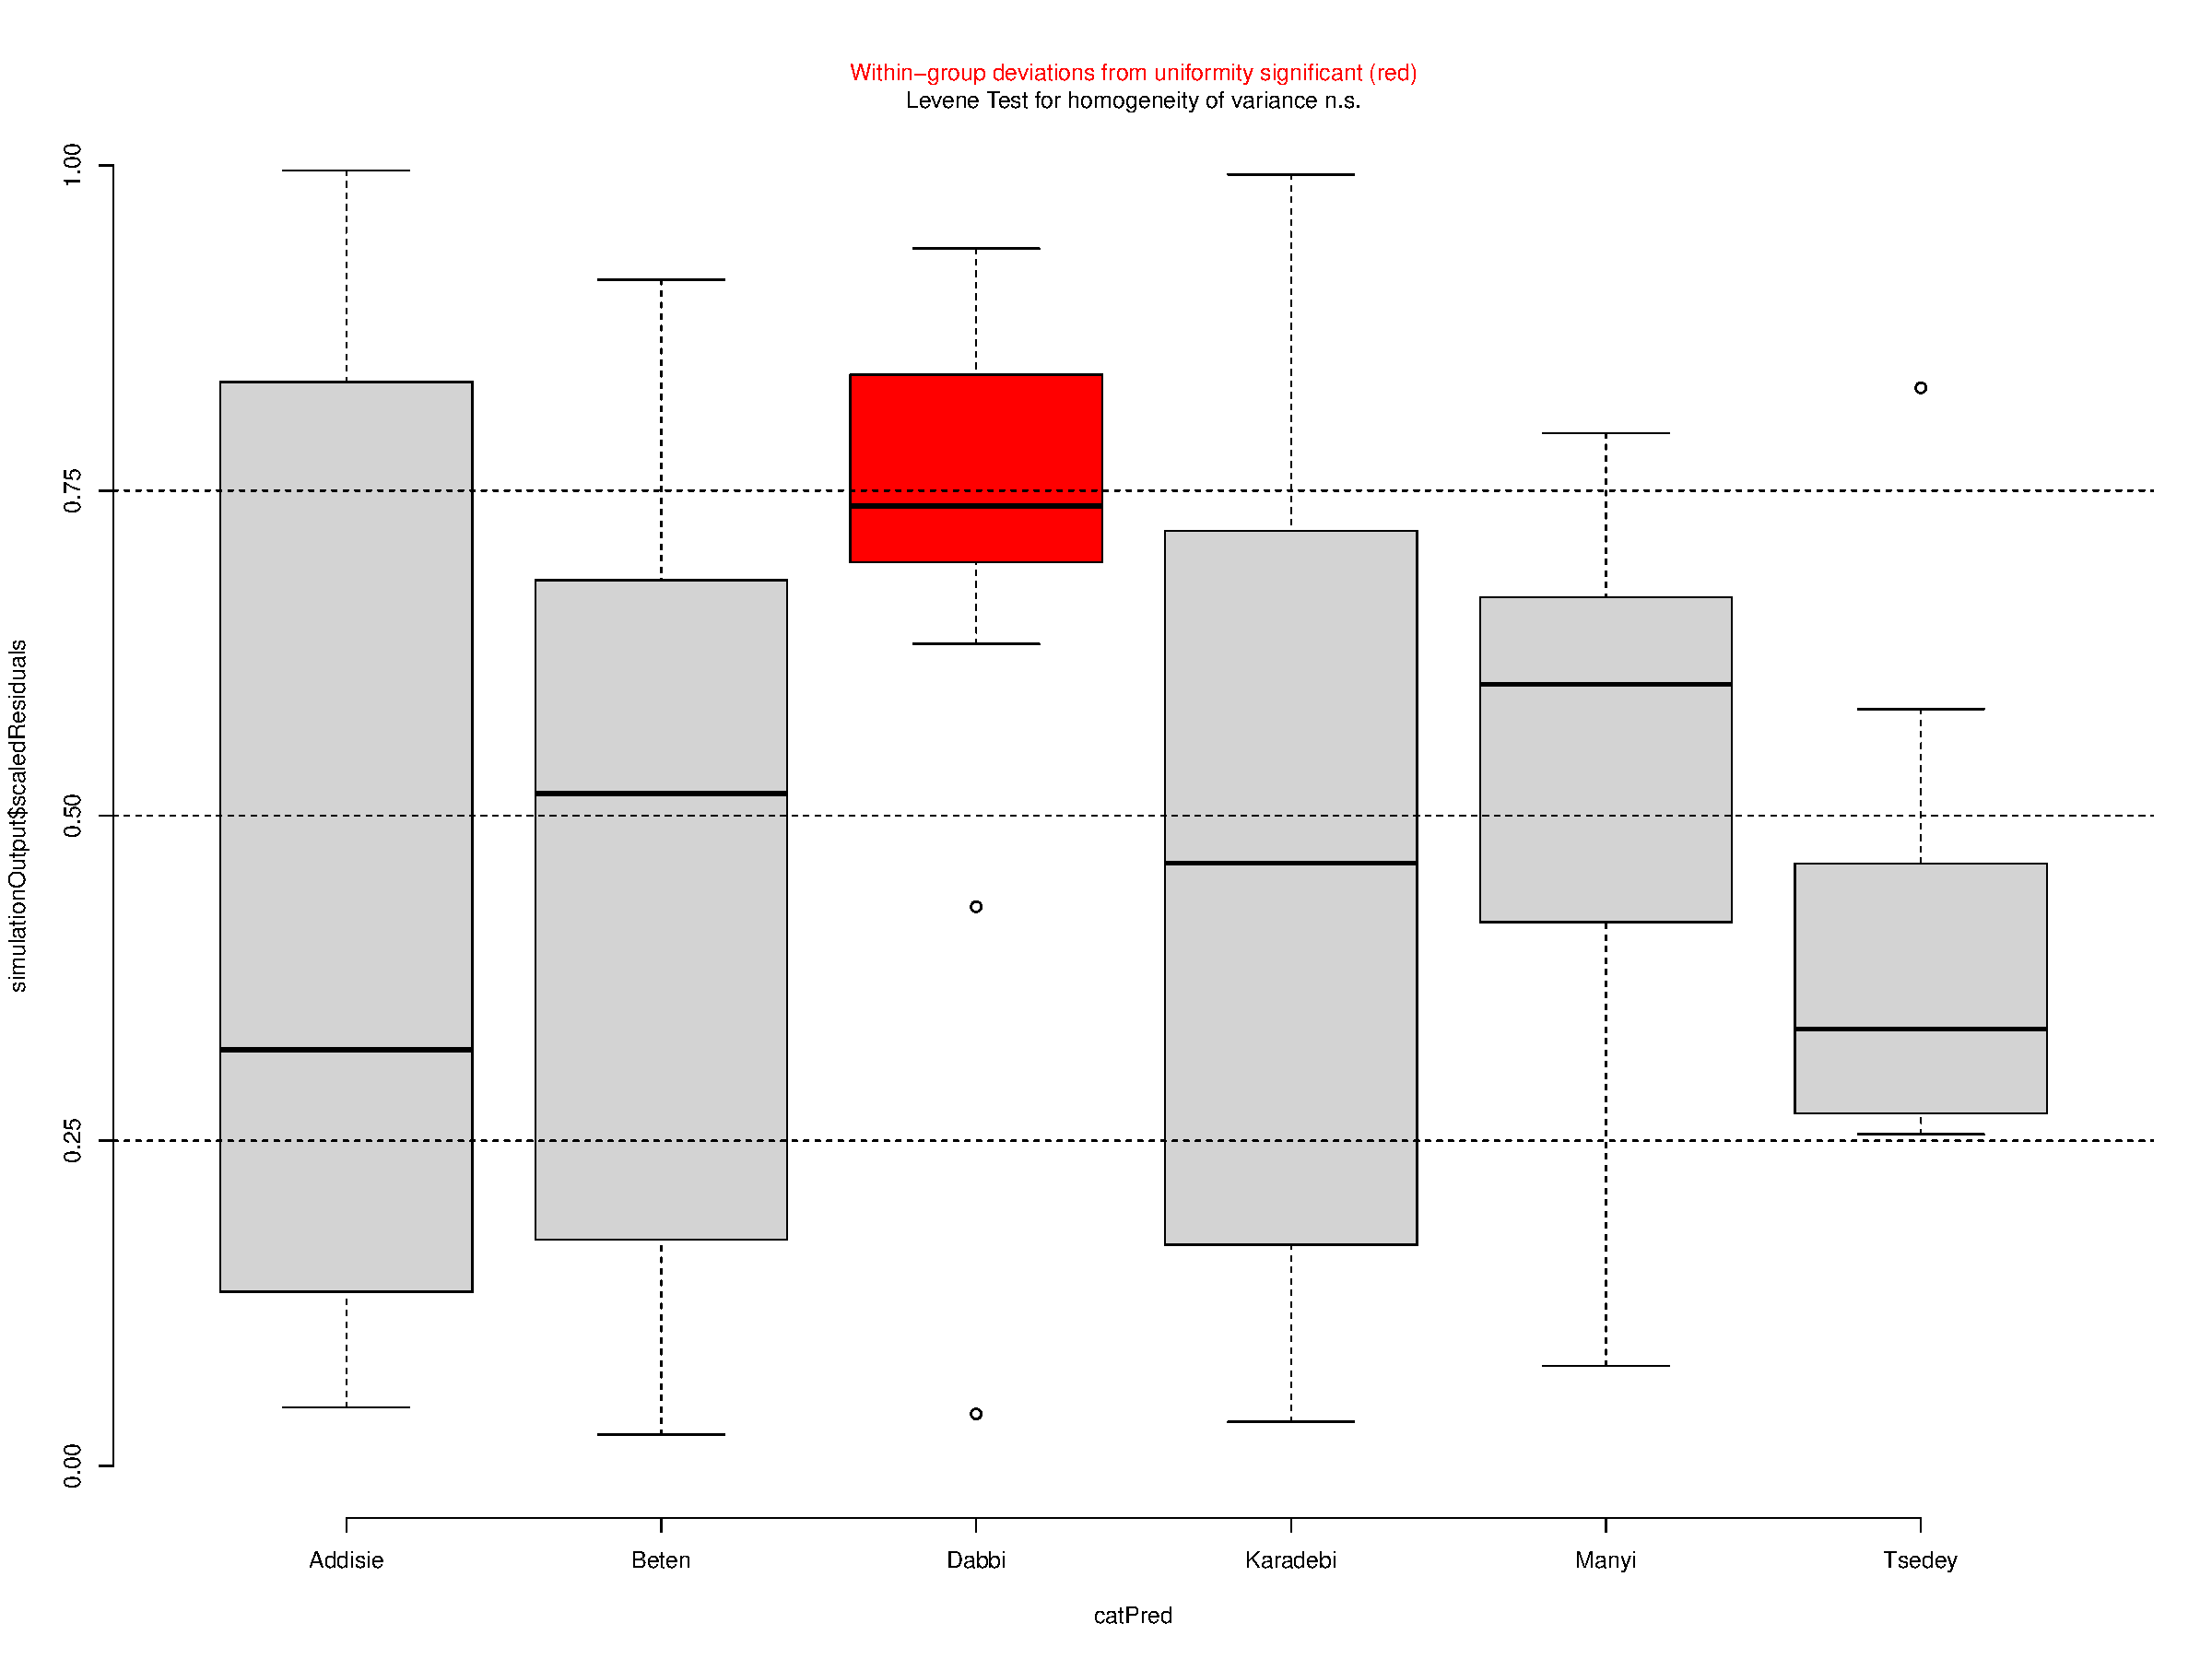
\includegraphics[keepaspectratio]{rsa_day1617_agar_files/figure-pdf/unnamed-chunk-12-9.pdf}}

\begin{Shaded}
\begin{Highlighting}[]
\CommentTok{\# overall fit with log transformation ooks better but there is within{-}group deviations from uniformity and non singular so will keep the non{-}log transformed model }

\NormalTok{Vol\_tmb }\OtherTok{\textless{}{-}} \FunctionTok{glmmTMB}\NormalTok{(}
\NormalTok{  Volume.mm3 }\SpecialCharTok{\textasciitilde{}}\NormalTok{ Genotype }\SpecialCharTok{+}\NormalTok{ (}\DecValTok{1} \SpecialCharTok{|}\NormalTok{ Batch}\SpecialCharTok{/}\NormalTok{Plate}\SpecialCharTok{/}\NormalTok{Seed),}
  \AttributeTok{data =}\NormalTok{ df, }
  \AttributeTok{family =} \FunctionTok{gaussian}\NormalTok{()}
\NormalTok{)}

\CommentTok{\# ── 5. Diagnostics: log model ────────────────────────────────}
\NormalTok{sim\_res\_vol }\OtherTok{\textless{}{-}} \FunctionTok{simulateResiduals}\NormalTok{(Vol\_tmb, }\AttributeTok{n =} \DecValTok{1000}\NormalTok{)}
\FunctionTok{plot}\NormalTok{(sim\_res\_vol)}
\end{Highlighting}
\end{Shaded}

\pandocbounded{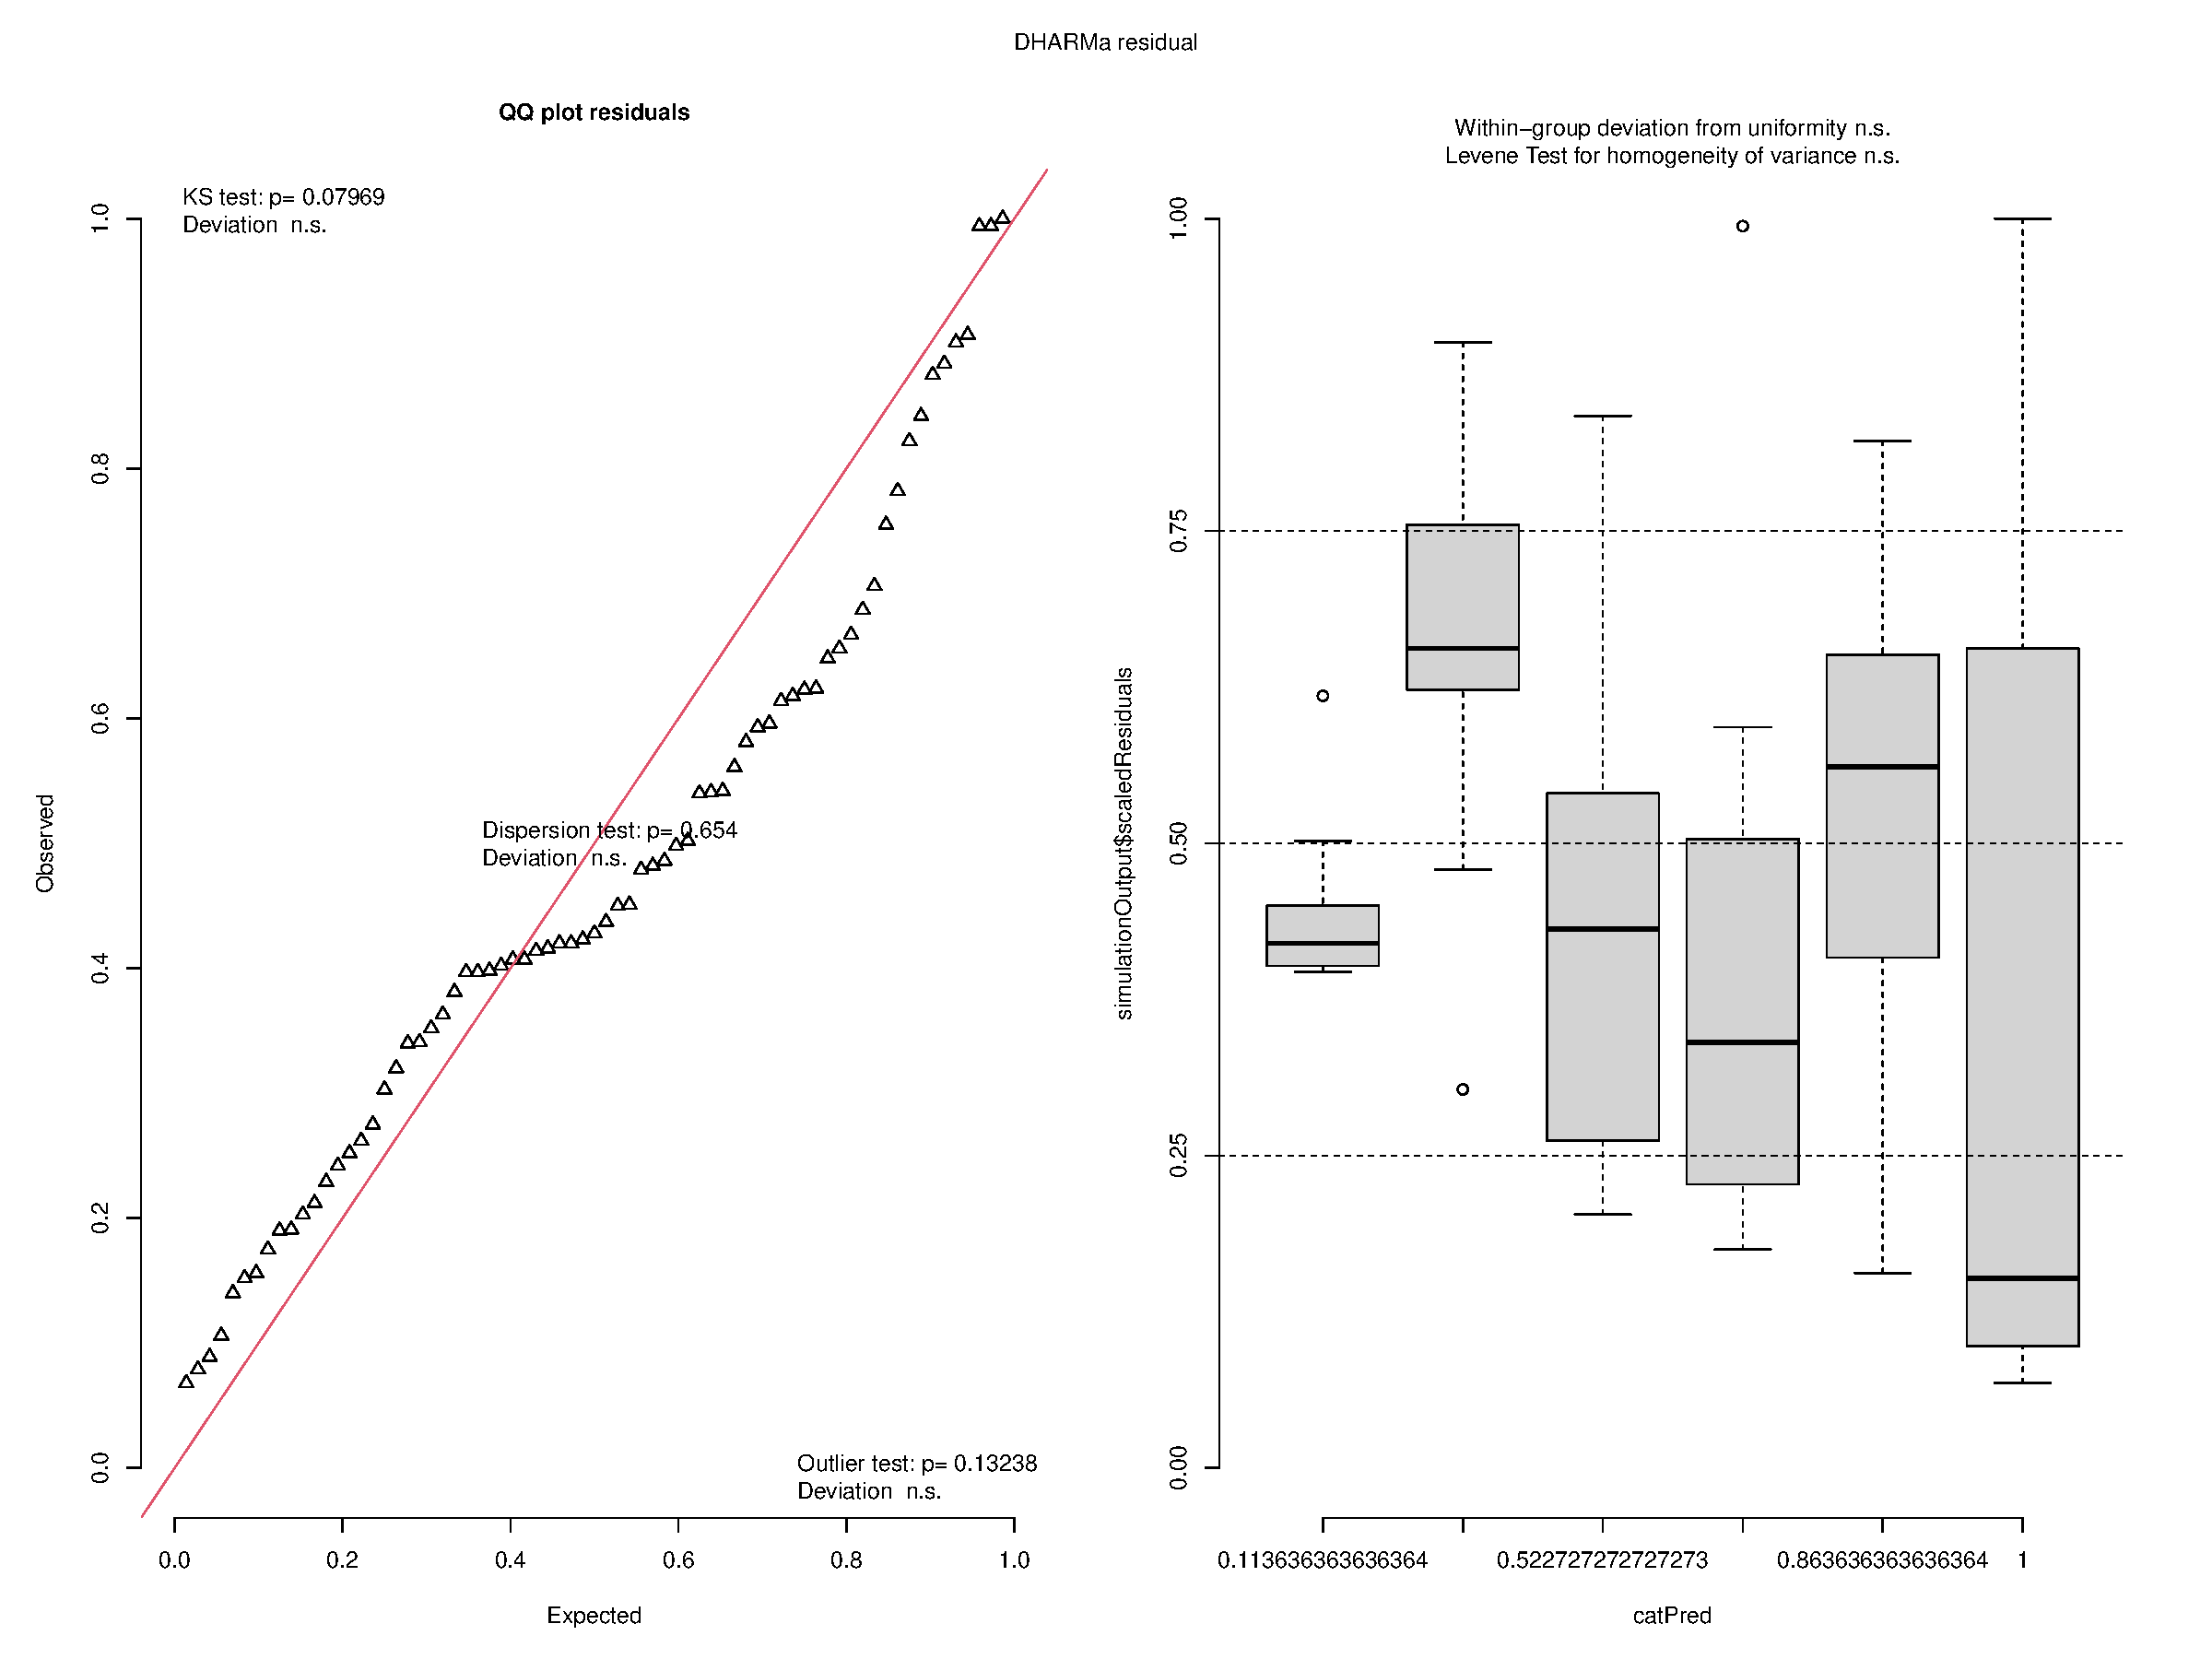
\includegraphics[keepaspectratio]{rsa_day1617_agar_files/figure-pdf/unnamed-chunk-12-10.pdf}}

\begin{Shaded}
\begin{Highlighting}[]
\FunctionTok{testUniformity}\NormalTok{(sim\_res\_vol)    }\CommentTok{\# p \textgreater{} 0.05 = good}
\end{Highlighting}
\end{Shaded}

\pandocbounded{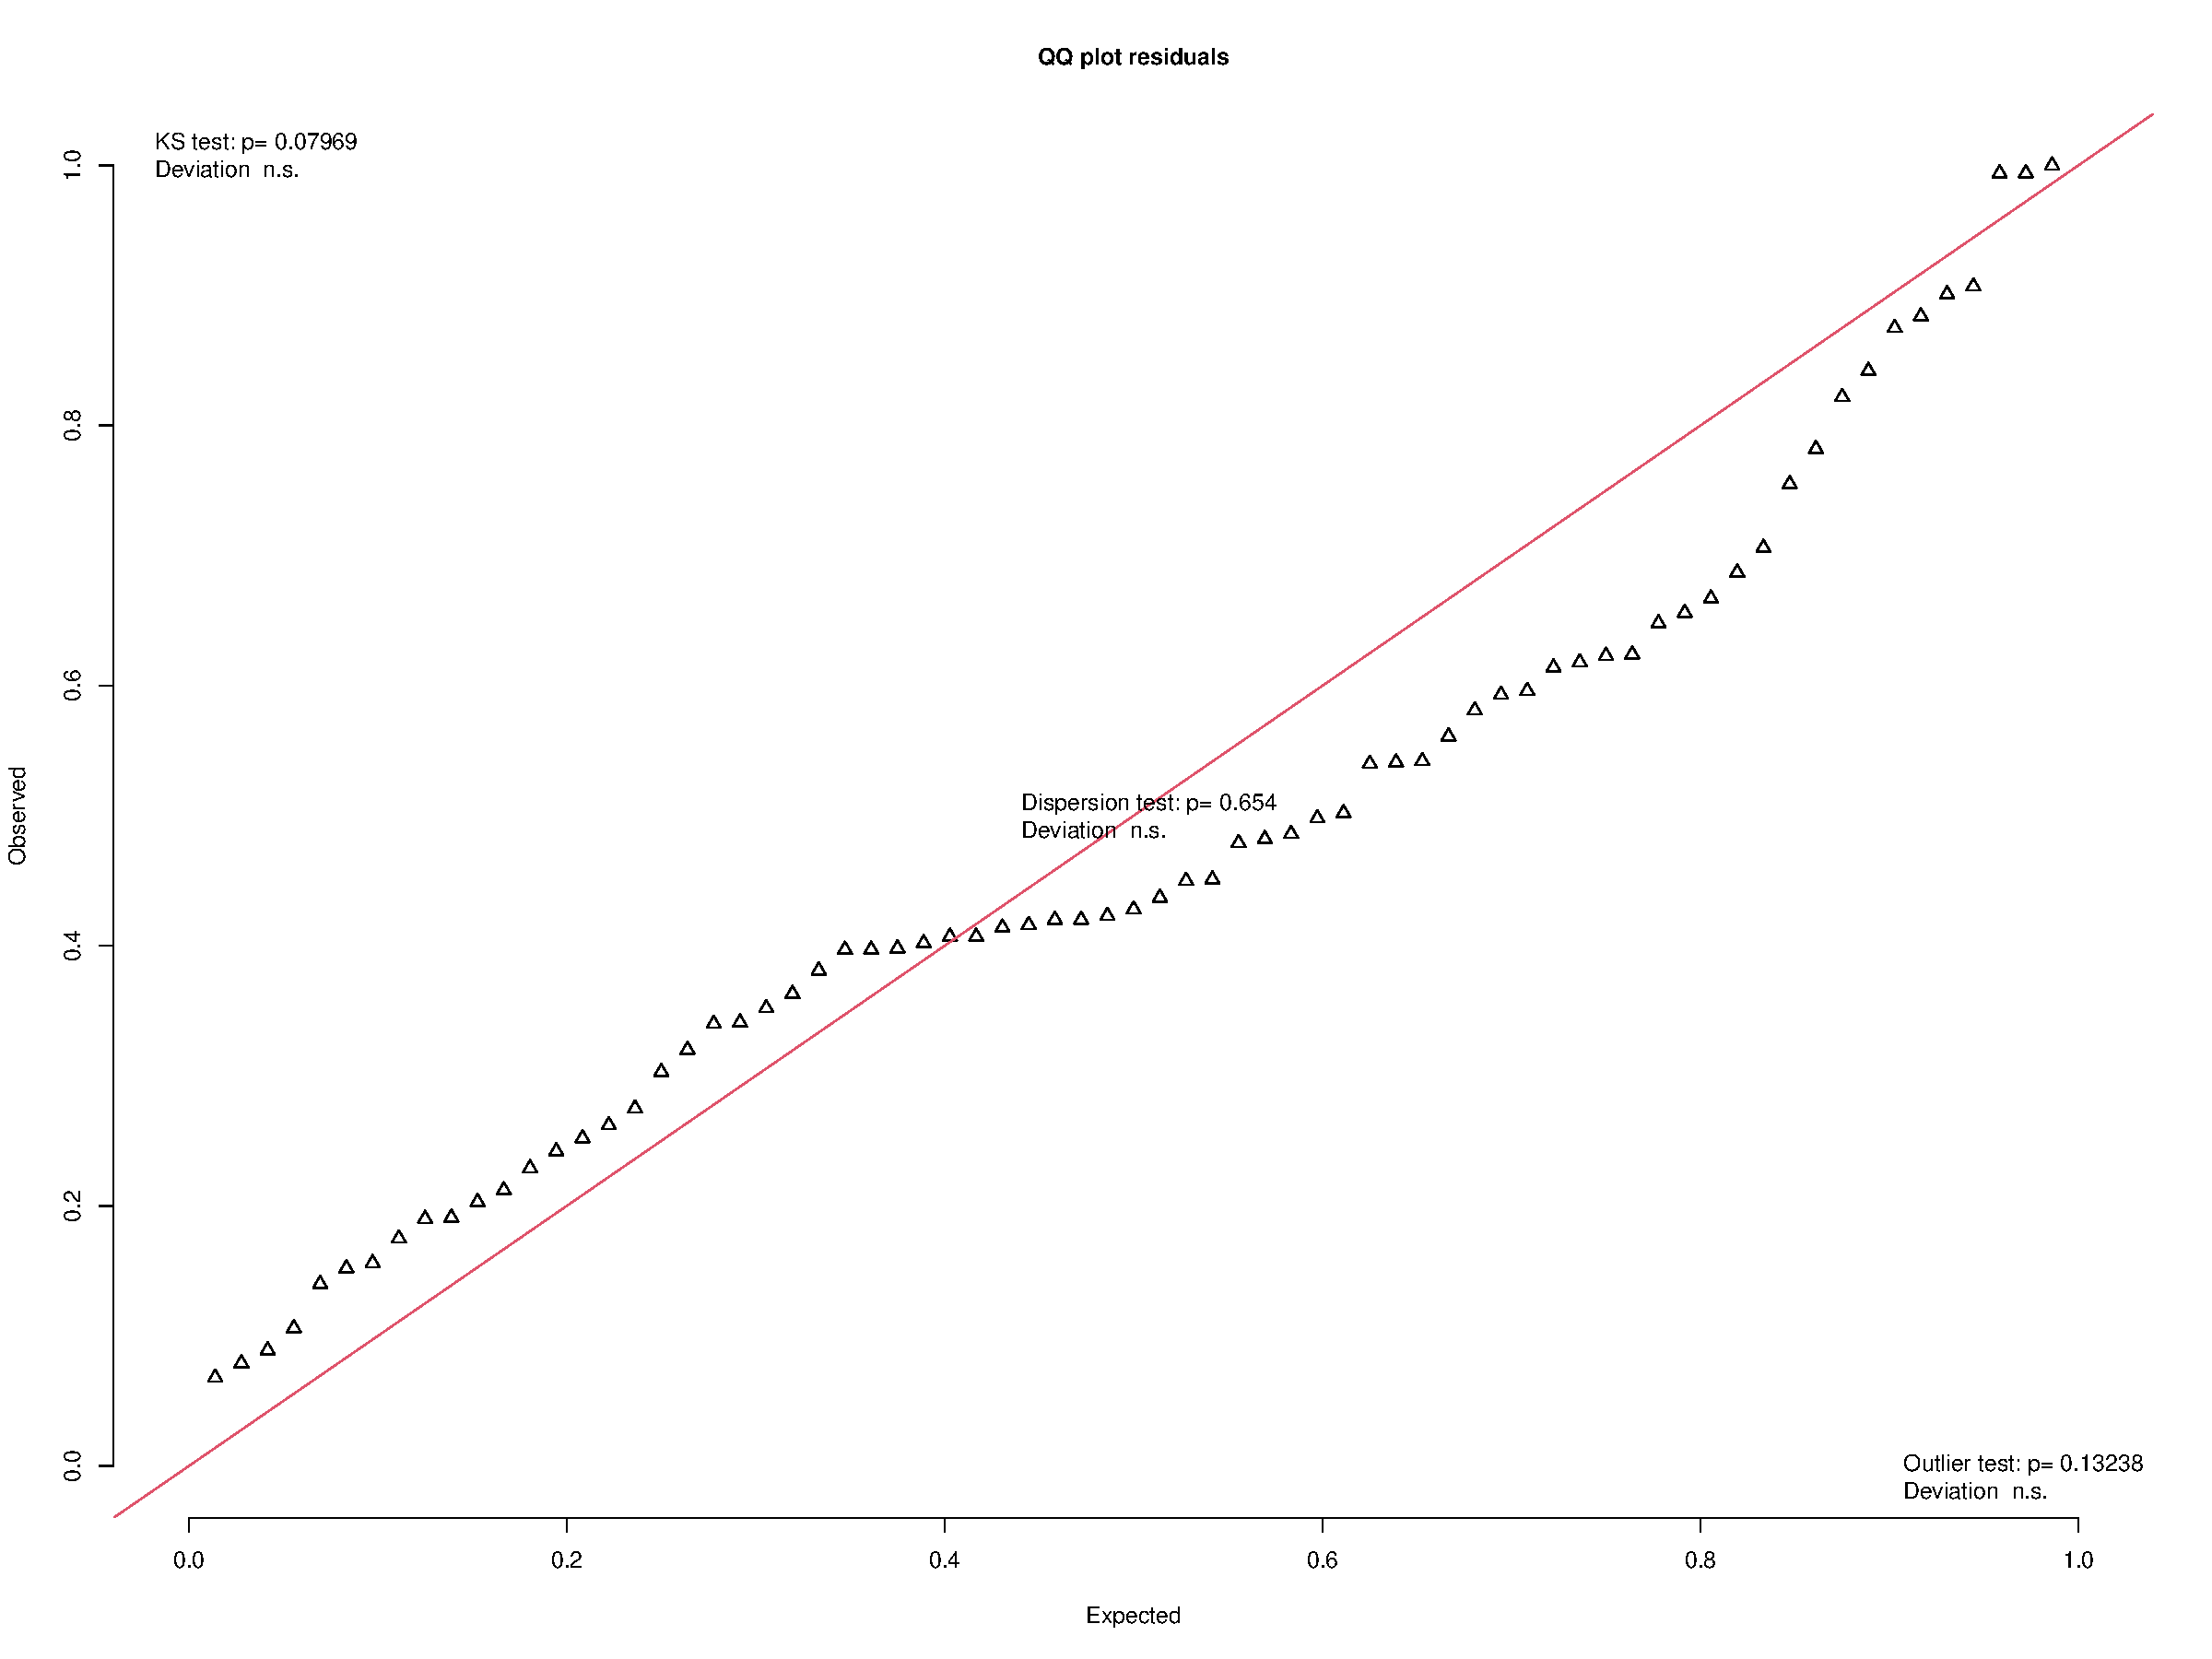
\includegraphics[keepaspectratio]{rsa_day1617_agar_files/figure-pdf/unnamed-chunk-12-11.pdf}}

\begin{verbatim}

    Asymptotic one-sample Kolmogorov-Smirnov test

data:  simulationOutput$scaledResiduals
D = 0.15065, p-value = 0.07969
alternative hypothesis: two-sided
\end{verbatim}

\begin{Shaded}
\begin{Highlighting}[]
\FunctionTok{testDispersion}\NormalTok{(sim\_res\_vol)    }\CommentTok{\# ratio ≈ 1.0}
\end{Highlighting}
\end{Shaded}

\pandocbounded{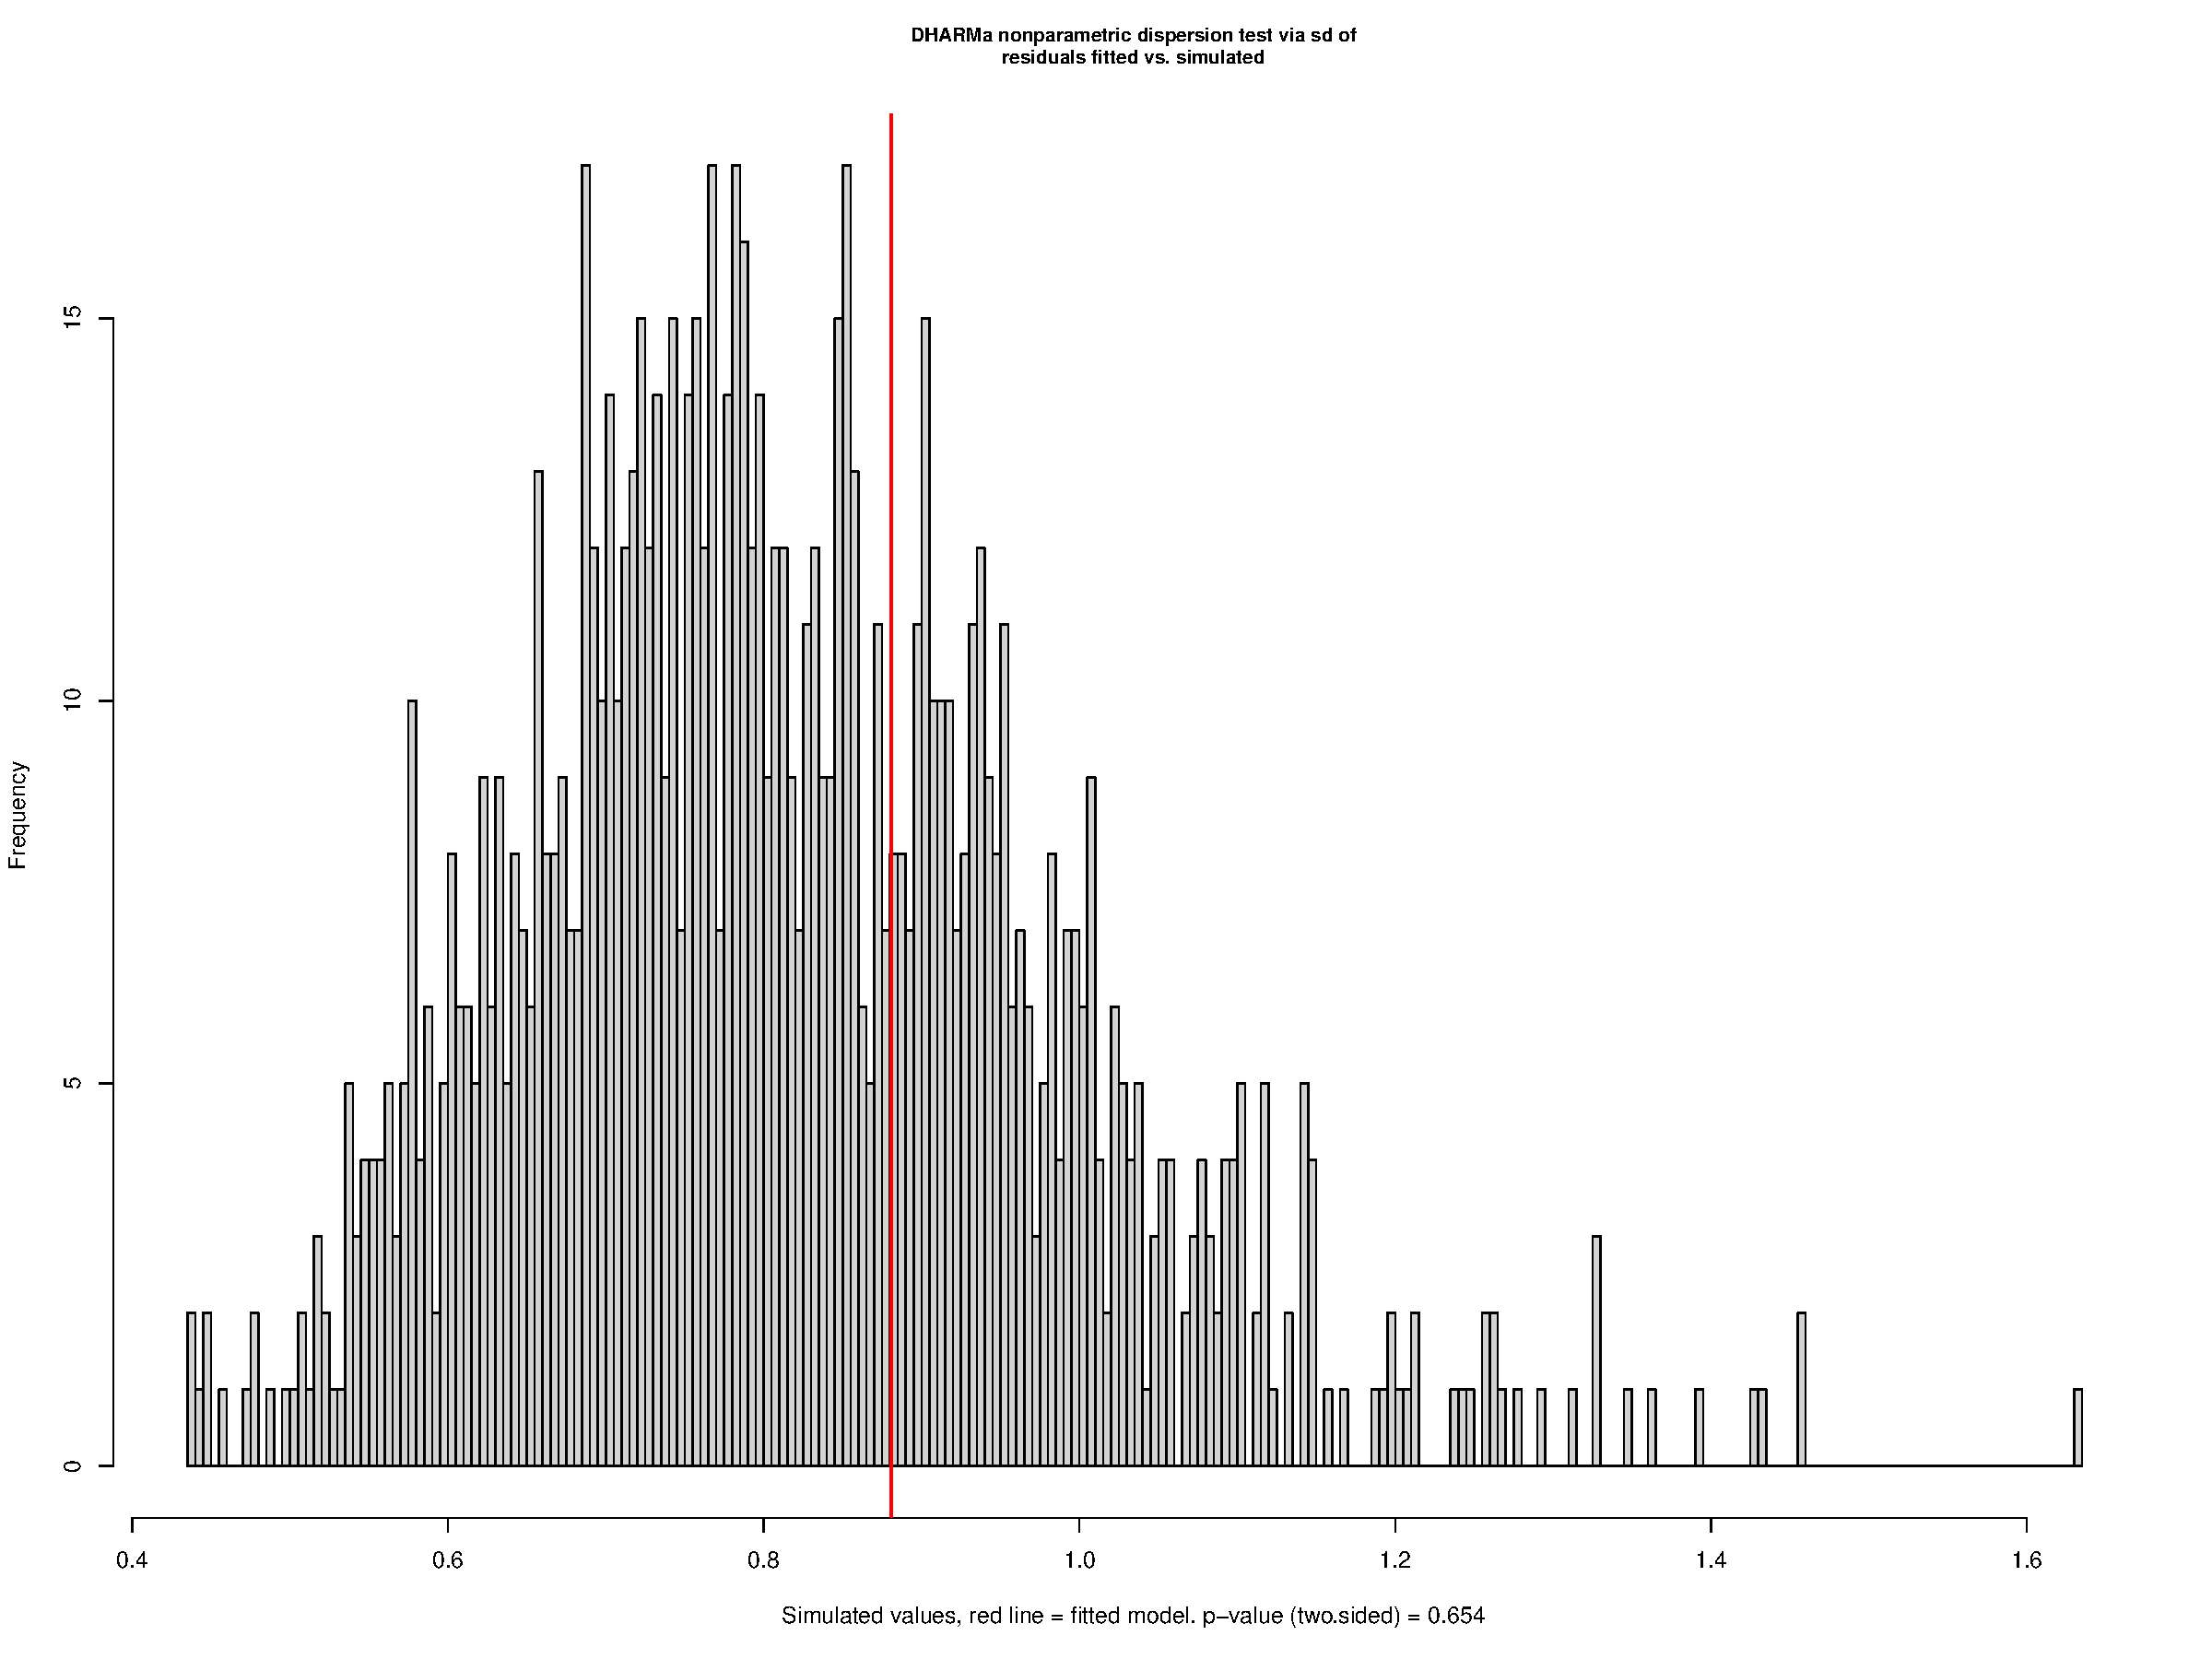
\includegraphics[keepaspectratio]{rsa_day1617_agar_files/figure-pdf/unnamed-chunk-12-12.pdf}}

\begin{verbatim}

    DHARMa nonparametric dispersion test via sd of residuals fitted vs.
    simulated

data:  simulationOutput
dispersion = 1.0777, p-value = 0.654
alternative hypothesis: two.sided
\end{verbatim}

\begin{Shaded}
\begin{Highlighting}[]
\FunctionTok{plotResiduals}\NormalTok{(sim\_res\_vol, }\AttributeTok{form =}\NormalTok{ df}\SpecialCharTok{$}\NormalTok{Genotype)}
\end{Highlighting}
\end{Shaded}

\pandocbounded{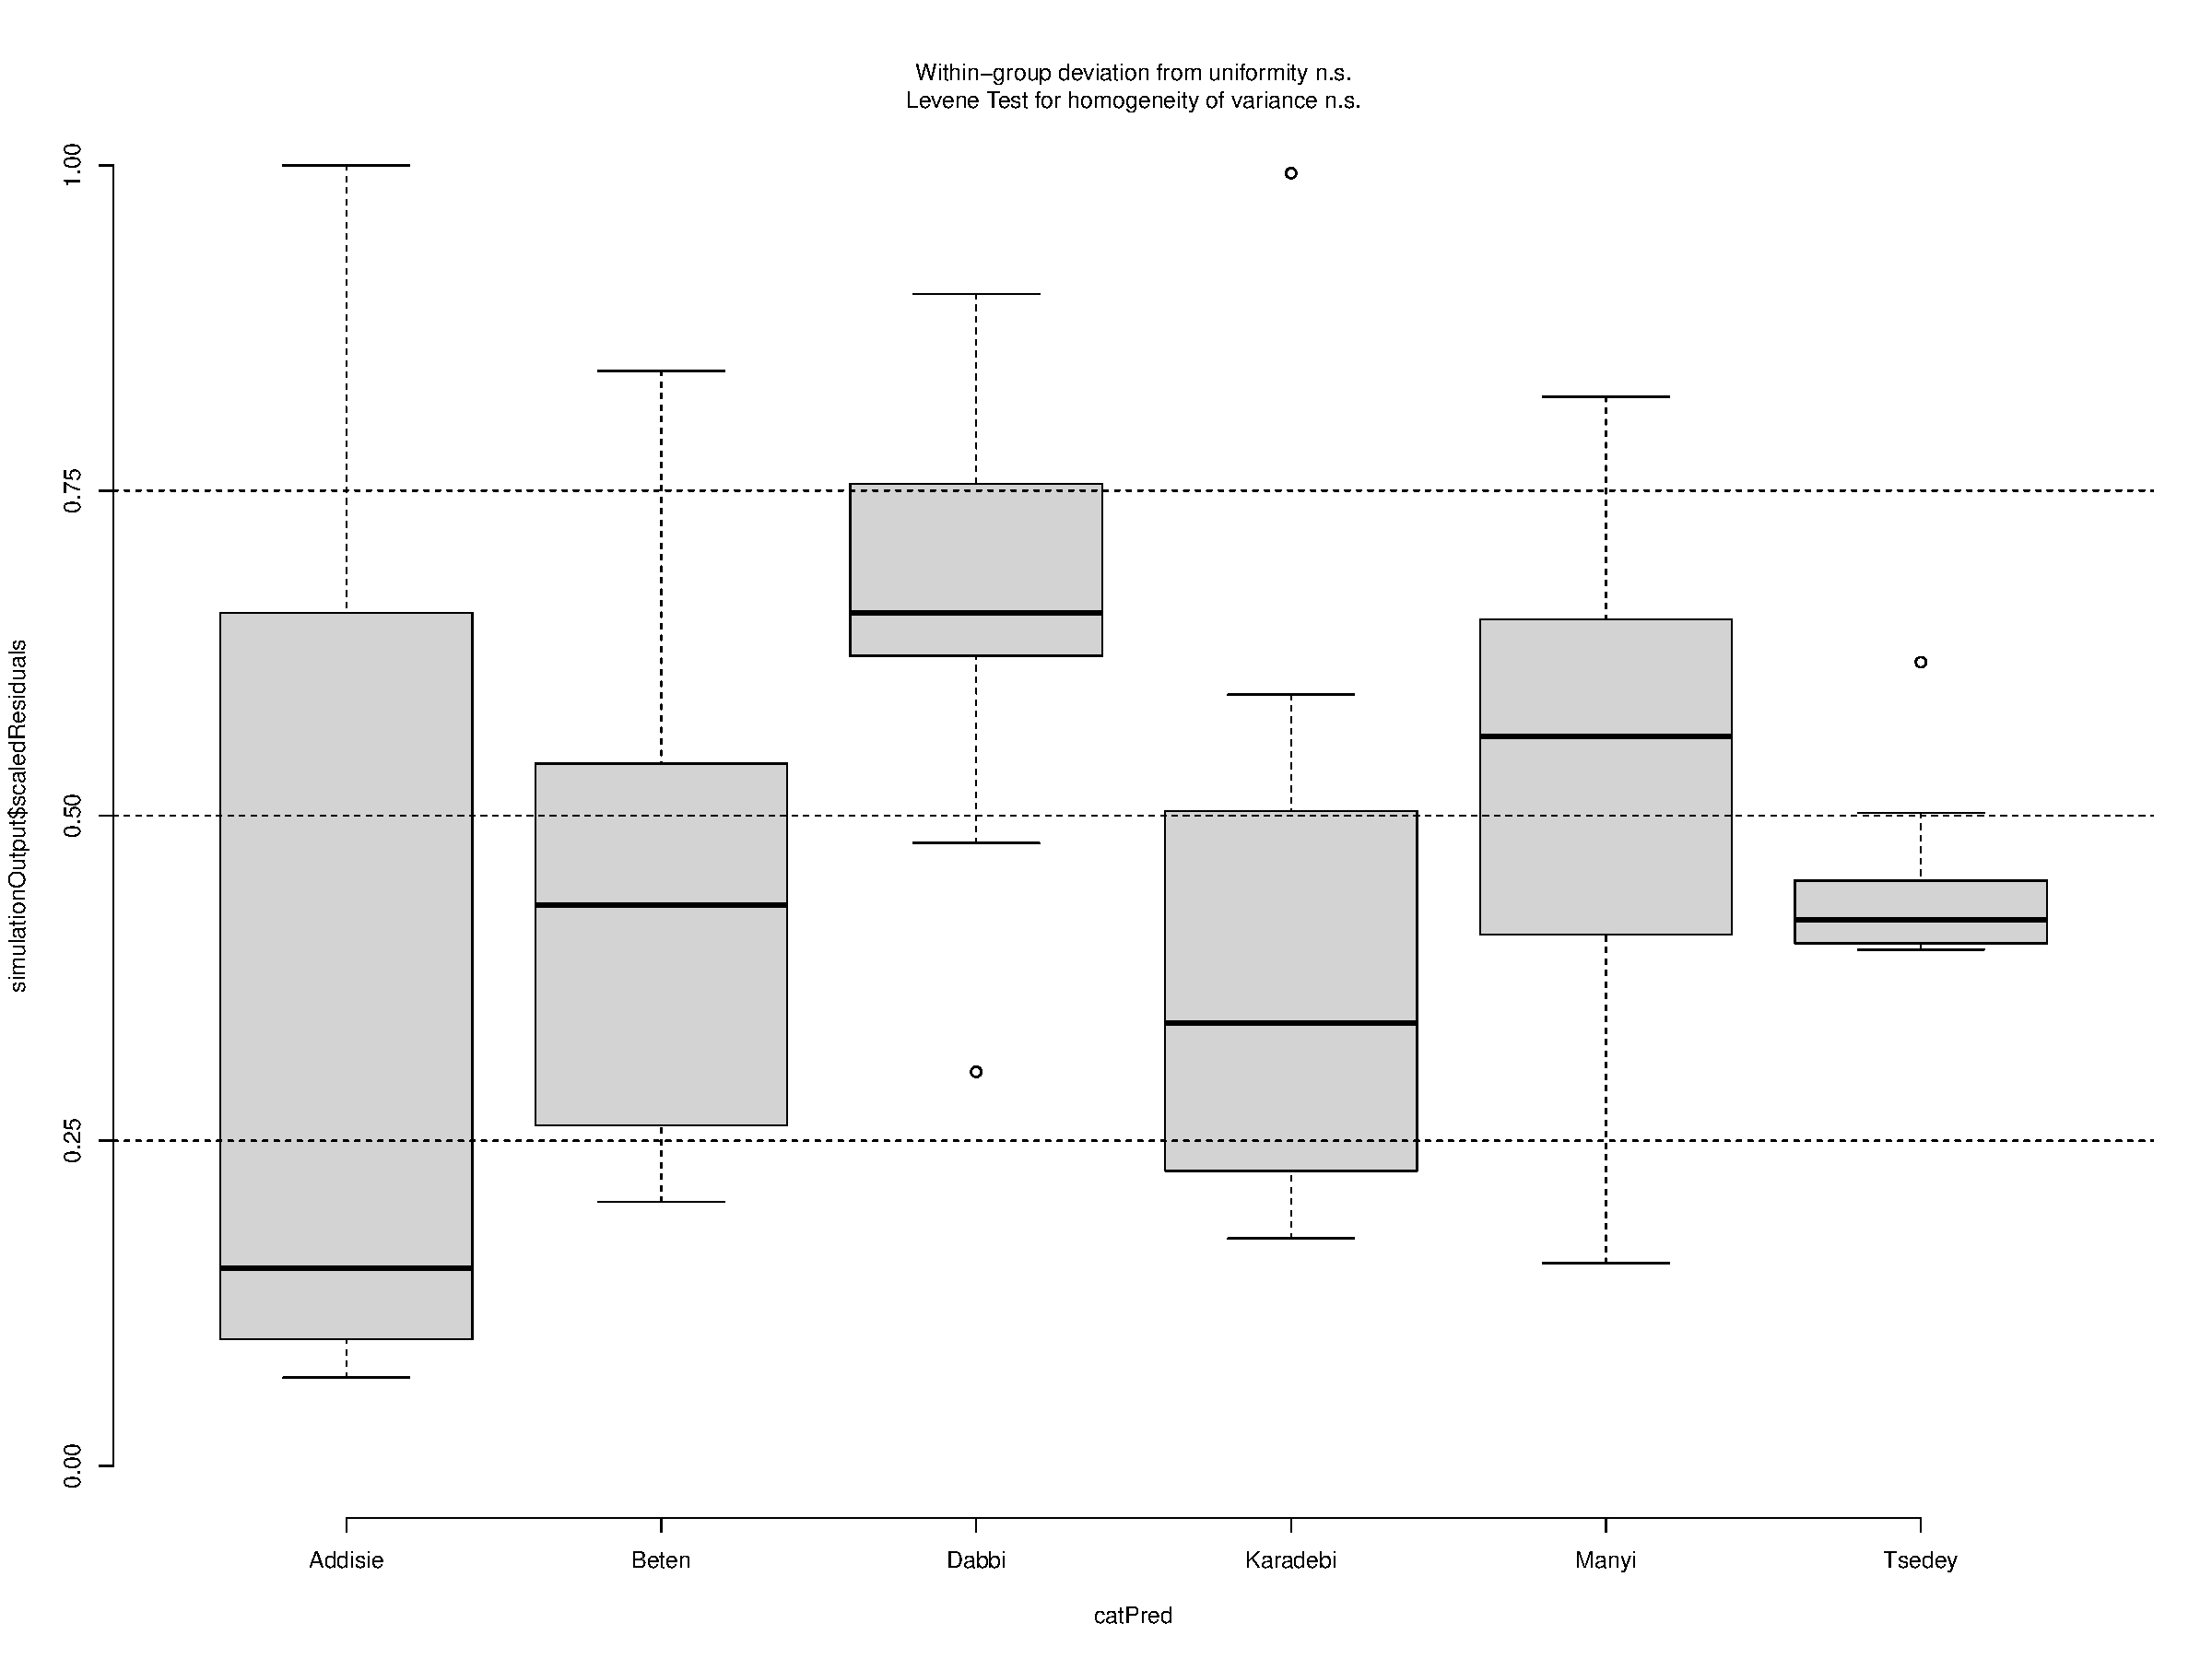
\includegraphics[keepaspectratio]{rsa_day1617_agar_files/figure-pdf/unnamed-chunk-12-13.pdf}}

\begin{Shaded}
\begin{Highlighting}[]
\NormalTok{car}\SpecialCharTok{::}\FunctionTok{Anova}\NormalTok{(Vol\_tmb, }\AttributeTok{type =} \StringTok{"III"}\NormalTok{)}
\end{Highlighting}
\end{Shaded}

\begin{verbatim}
Analysis of Deviance Table (Type III Wald chisquare tests)

Response: Volume.mm3
             Chisq Df Pr(>Chisq)    
(Intercept) 24.530  1  7.315e-07 ***
Genotype    13.292  5    0.02079 *  
---
Signif. codes:  0 '***' 0.001 '**' 0.01 '*' 0.05 '.' 0.1 ' ' 1
\end{verbatim}

\begin{Shaded}
\begin{Highlighting}[]
\CommentTok{\# Pairwise (type = "response" ONLY if using log model)}
\NormalTok{emm }\OtherTok{\textless{}{-}} \FunctionTok{emmeans}\NormalTok{(Vol\_tmb, }\SpecialCharTok{\textasciitilde{}}\NormalTok{ Genotype, }
               \AttributeTok{type =} \StringTok{"response"}\NormalTok{)}
\FunctionTok{pairs}\NormalTok{(emm, }\AttributeTok{adjust =} \StringTok{"sidak"}\NormalTok{)}
\end{Highlighting}
\end{Shaded}

\begin{verbatim}
 contrast           estimate   SE  df z.ratio p.value
 Addisie - Beten       7.432 3.49 Inf   2.127  0.3991
 Addisie - Dabbi      10.048 4.13 Inf   2.433  0.2024
 Addisie - Karadebi    5.801 3.87 Inf   1.500  0.8837
 Addisie - Manyi       2.201 4.53 Inf   0.486  1.0000
 Addisie - Tsedey     11.014 3.74 Inf   2.945  0.0473
 Beten - Dabbi         2.616 3.88 Inf   0.674  1.0000
 Beten - Karadebi     -1.630 3.63 Inf  -0.449  1.0000
 Beten - Manyi        -5.230 4.23 Inf  -1.236  0.9743
 Beten - Tsedey        3.582 3.33 Inf   1.076  0.9931
 Dabbi - Karadebi     -4.246 3.59 Inf  -1.182  0.9828
 Dabbi - Manyi        -7.846 4.13 Inf  -1.899  0.5889
 Dabbi - Tsedey        0.966 3.89 Inf   0.249  1.0000
 Karadebi - Manyi     -3.600 4.05 Inf  -0.888  0.9991
 Karadebi - Tsedey     5.212 3.70 Inf   1.410  0.9251
 Manyi - Tsedey        8.812 4.10 Inf   2.148  0.3834

P value adjustment: sidak method for 15 tests 
\end{verbatim}

\begin{Shaded}
\begin{Highlighting}[]
\CommentTok{\# Cohen\textquotesingle{}s d = difference in means / pooled SD}
\CommentTok{\# Interpretation: 0.2 = small, 0.5 = medium, 0.8 = large}

\NormalTok{eff\_vol }\OtherTok{\textless{}{-}} \FunctionTok{eff\_size}\NormalTok{(}
\NormalTok{  emm,}
  \AttributeTok{sigma =} \FunctionTok{sigma}\NormalTok{(Vol\_tmb),   }\CommentTok{\# residual SD from model}
  \AttributeTok{edf   =} \FunctionTok{df.residual}\NormalTok{(Vol\_tmb)}
\NormalTok{)}
\FunctionTok{print}\NormalTok{(eff\_vol)}
\end{Highlighting}
\end{Shaded}

\begin{verbatim}
 contrast           estimate    SE  df asymp.LCL asymp.UCL
 Addisie - Beten       0.902 0.432 Inf    0.0557    1.7485
 Addisie - Dabbi       1.220 0.513 Inf    0.2137    2.2257
 Addisie - Karadebi    0.704 0.474 Inf   -0.2245    1.6330
 Addisie - Manyi       0.267 0.551 Inf   -0.8118    1.3463
 Addisie - Tsedey      1.337 0.470 Inf    0.4162    2.2578
 Beten - Dabbi         0.318 0.472 Inf   -0.6082    1.2434
 Beten - Karadebi     -0.198 0.441 Inf   -1.0623    0.6665
 Beten - Manyi        -0.635 0.517 Inf   -1.6483    0.3784
 Beten - Tsedey        0.435 0.406 Inf   -0.3613    1.2310
 Dabbi - Karadebi     -0.515 0.439 Inf   -1.3750    0.3441
 Dabbi - Manyi        -0.952 0.509 Inf   -1.9498    0.0449
 Dabbi - Tsedey        0.117 0.472 Inf   -0.8073    1.0419
 Karadebi - Manyi     -0.437 0.494 Inf   -1.4044    0.5303
 Karadebi - Tsedey     0.633 0.453 Inf   -0.2542    1.5196
 Manyi - Tsedey        1.070 0.507 Inf    0.0753    2.0642

sigma used for effect sizes: 8.238 
Confidence level used: 0.95 
\end{verbatim}

\begin{Shaded}
\begin{Highlighting}[]
\CommentTok{\# ── 8. CLD and sample sizes ──────────────────────────────────}
\NormalTok{cld\_df }\OtherTok{\textless{}{-}} \FunctionTok{as.data.frame}\NormalTok{(}\FunctionTok{cld}\NormalTok{(emm, }\AttributeTok{adjust =} \StringTok{"sidak"}\NormalTok{,}
                             \AttributeTok{Letters =}\NormalTok{ letters, }\AttributeTok{alpha =} \FloatTok{0.05}\NormalTok{)) }\SpecialCharTok{\%\textgreater{}\%}
  \FunctionTok{mutate}\NormalTok{(}\AttributeTok{.group =} \FunctionTok{trimws}\NormalTok{(.group))}

\NormalTok{n\_df }\OtherTok{\textless{}{-}}\NormalTok{ df }\SpecialCharTok{\%\textgreater{}\%}
  \FunctionTok{count}\NormalTok{(Genotype) }\SpecialCharTok{\%\textgreater{}\%}
  \FunctionTok{mutate}\NormalTok{(}\AttributeTok{label =} \FunctionTok{paste0}\NormalTok{(}\StringTok{"n="}\NormalTok{, n))}

\CommentTok{\# ── 9. Plot — Boxplot ────────────────────────────────────────}

\NormalTok{y\_ceil }\OtherTok{\textless{}{-}} \FunctionTok{max}\NormalTok{(df}\SpecialCharTok{$}\NormalTok{Volume.mm3) }\SpecialCharTok{*} \FloatTok{1.22}
\NormalTok{y\_label }\OtherTok{\textless{}{-}}\NormalTok{ y\_ceil }\SpecialCharTok{*} \FloatTok{0.95}

\NormalTok{p1 }\OtherTok{\textless{}{-}} \FunctionTok{ggplot}\NormalTok{(df, }\FunctionTok{aes}\NormalTok{(}\AttributeTok{x =}\NormalTok{ Genotype, }\AttributeTok{y =}\NormalTok{ Volume.mm3, }\AttributeTok{fill =}\NormalTok{ Genotype)) }\SpecialCharTok{+}
  
  \FunctionTok{geom\_boxplot}\NormalTok{(}
    \AttributeTok{alpha         =} \FloatTok{0.7}\NormalTok{,}
    \AttributeTok{outlier.shape =} \ConstantTok{NA}\NormalTok{,}
    \AttributeTok{width         =} \FloatTok{0.5}\NormalTok{,}
    \AttributeTok{colour        =} \StringTok{"black"}\NormalTok{,}
    \AttributeTok{linewidth     =} \FloatTok{0.5}
\NormalTok{  ) }\SpecialCharTok{+}
  
  \FunctionTok{geom\_jitter}\NormalTok{(}
    \AttributeTok{width  =} \FloatTok{0.15}\NormalTok{,}
    \AttributeTok{size   =} \FloatTok{1.8}\NormalTok{,}
    \AttributeTok{alpha  =} \FloatTok{0.55}\NormalTok{,}
    \AttributeTok{colour =} \StringTok{"black"}
\NormalTok{  ) }\SpecialCharTok{+}
  
  \FunctionTok{geom\_text}\NormalTok{(}
    \AttributeTok{data        =}\NormalTok{ cld\_df,}
    \FunctionTok{aes}\NormalTok{(}\AttributeTok{x =}\NormalTok{ Genotype, }\AttributeTok{label =}\NormalTok{ .group),}
    \AttributeTok{y           =}\NormalTok{ y\_label,}
    \AttributeTok{inherit.aes =} \ConstantTok{FALSE}\NormalTok{,}
    \AttributeTok{size        =} \DecValTok{8}\NormalTok{,}
    \AttributeTok{fontface    =} \StringTok{"bold"}\NormalTok{,}
    \AttributeTok{colour      =} \StringTok{"grey20"}
\NormalTok{  ) }\SpecialCharTok{+}
  
  \FunctionTok{geom\_text}\NormalTok{(}
    \AttributeTok{data        =}\NormalTok{ n\_df,}
    \FunctionTok{aes}\NormalTok{(}\AttributeTok{x =}\NormalTok{ Genotype, }\AttributeTok{label =}\NormalTok{ label),}
    \AttributeTok{y           =} \SpecialCharTok{{-}}\ConstantTok{Inf}\NormalTok{,}
    \AttributeTok{vjust       =} \FloatTok{4.2}\NormalTok{,}
    \AttributeTok{inherit.aes =} \ConstantTok{FALSE}\NormalTok{,}
    \AttributeTok{size        =} \DecValTok{6}\NormalTok{,}
    \AttributeTok{colour      =} \StringTok{"grey40"}
\NormalTok{  ) }\SpecialCharTok{+}
  
  \FunctionTok{scale\_fill\_brewer}\NormalTok{(}\AttributeTok{palette =} \StringTok{"Set2"}\NormalTok{) }\SpecialCharTok{+}

  \FunctionTok{labs}\NormalTok{(}
    \AttributeTok{x       =} \StringTok{"Genotype"}\NormalTok{,}
    \AttributeTok{y       =} \StringTok{"Volume (mm³)"}\NormalTok{,}
    \AttributeTok{caption =} \StringTok{"Shared letters indicate no significant difference (sidak HSD, p \textgreater{} 0.05; glmmTMB, Gaussian)"}
\NormalTok{  ) }\SpecialCharTok{+}
  
  \FunctionTok{theme\_classic}\NormalTok{(}\AttributeTok{base\_size =} \DecValTok{14}\NormalTok{) }\SpecialCharTok{+}
  \FunctionTok{theme}\NormalTok{(}
    \AttributeTok{legend.position =} \StringTok{"none"}\NormalTok{,}
    \AttributeTok{panel.grid      =} \FunctionTok{element\_blank}\NormalTok{(),}
    \AttributeTok{axis.line       =} \FunctionTok{element\_line}\NormalTok{(}\AttributeTok{colour =} \StringTok{"black"}\NormalTok{, }\AttributeTok{linewidth =} \FloatTok{0.6}\NormalTok{),}
    \AttributeTok{axis.ticks      =} \FunctionTok{element\_line}\NormalTok{(}\AttributeTok{colour =} \StringTok{"black"}\NormalTok{, }\AttributeTok{linewidth =} \FloatTok{0.5}\NormalTok{),}
    \AttributeTok{axis.title      =} \FunctionTok{element\_text}\NormalTok{(}\AttributeTok{size =} \DecValTok{26}\NormalTok{, }\AttributeTok{face =} \StringTok{"bold"}\NormalTok{),}
    \AttributeTok{axis.title.x    =} \FunctionTok{element\_text}\NormalTok{(}\AttributeTok{size =} \DecValTok{26}\NormalTok{, }\AttributeTok{face =} \StringTok{"bold"}\NormalTok{, }\AttributeTok{margin =} \FunctionTok{margin}\NormalTok{(}\AttributeTok{t =} \DecValTok{24}\NormalTok{)),}
    \AttributeTok{axis.text       =} \FunctionTok{element\_text}\NormalTok{(}\AttributeTok{size =} \DecValTok{22}\NormalTok{, }\AttributeTok{colour =} \StringTok{"black"}\NormalTok{),}
    \AttributeTok{axis.text.x     =} \FunctionTok{element\_text}\NormalTok{(}\AttributeTok{face =} \StringTok{"italic"}\NormalTok{, }\AttributeTok{margin =} \FunctionTok{margin}\NormalTok{(}\AttributeTok{t =} \DecValTok{15}\NormalTok{)),}
    \AttributeTok{plot.caption    =} \FunctionTok{element\_text}\NormalTok{(}\AttributeTok{size =} \DecValTok{12}\NormalTok{, }\AttributeTok{colour =} \StringTok{"grey40"}\NormalTok{, }\AttributeTok{hjust =} \DecValTok{0}\NormalTok{, }\AttributeTok{margin =} \FunctionTok{margin}\NormalTok{(}\AttributeTok{t =} \DecValTok{10}\NormalTok{)),}
    \AttributeTok{plot.margin     =} \FunctionTok{margin}\NormalTok{(}\AttributeTok{t =} \DecValTok{25}\NormalTok{, }\AttributeTok{r =} \DecValTok{25}\NormalTok{, }\AttributeTok{b =} \DecValTok{25}\NormalTok{, }\AttributeTok{l =} \DecValTok{25}\NormalTok{)}
\NormalTok{  )}

\NormalTok{p1 }\SpecialCharTok{+} \FunctionTok{coord\_cartesian}\NormalTok{(}
  \AttributeTok{ylim =} \FunctionTok{c}\NormalTok{(}\DecValTok{0}\NormalTok{, }\FunctionTok{max}\NormalTok{(df}\SpecialCharTok{$}\NormalTok{Volume.mm3) }\SpecialCharTok{*} \FloatTok{1.22}\NormalTok{),}
  \AttributeTok{clip =} \StringTok{"off"}
\NormalTok{)}
\end{Highlighting}
\end{Shaded}

\pandocbounded{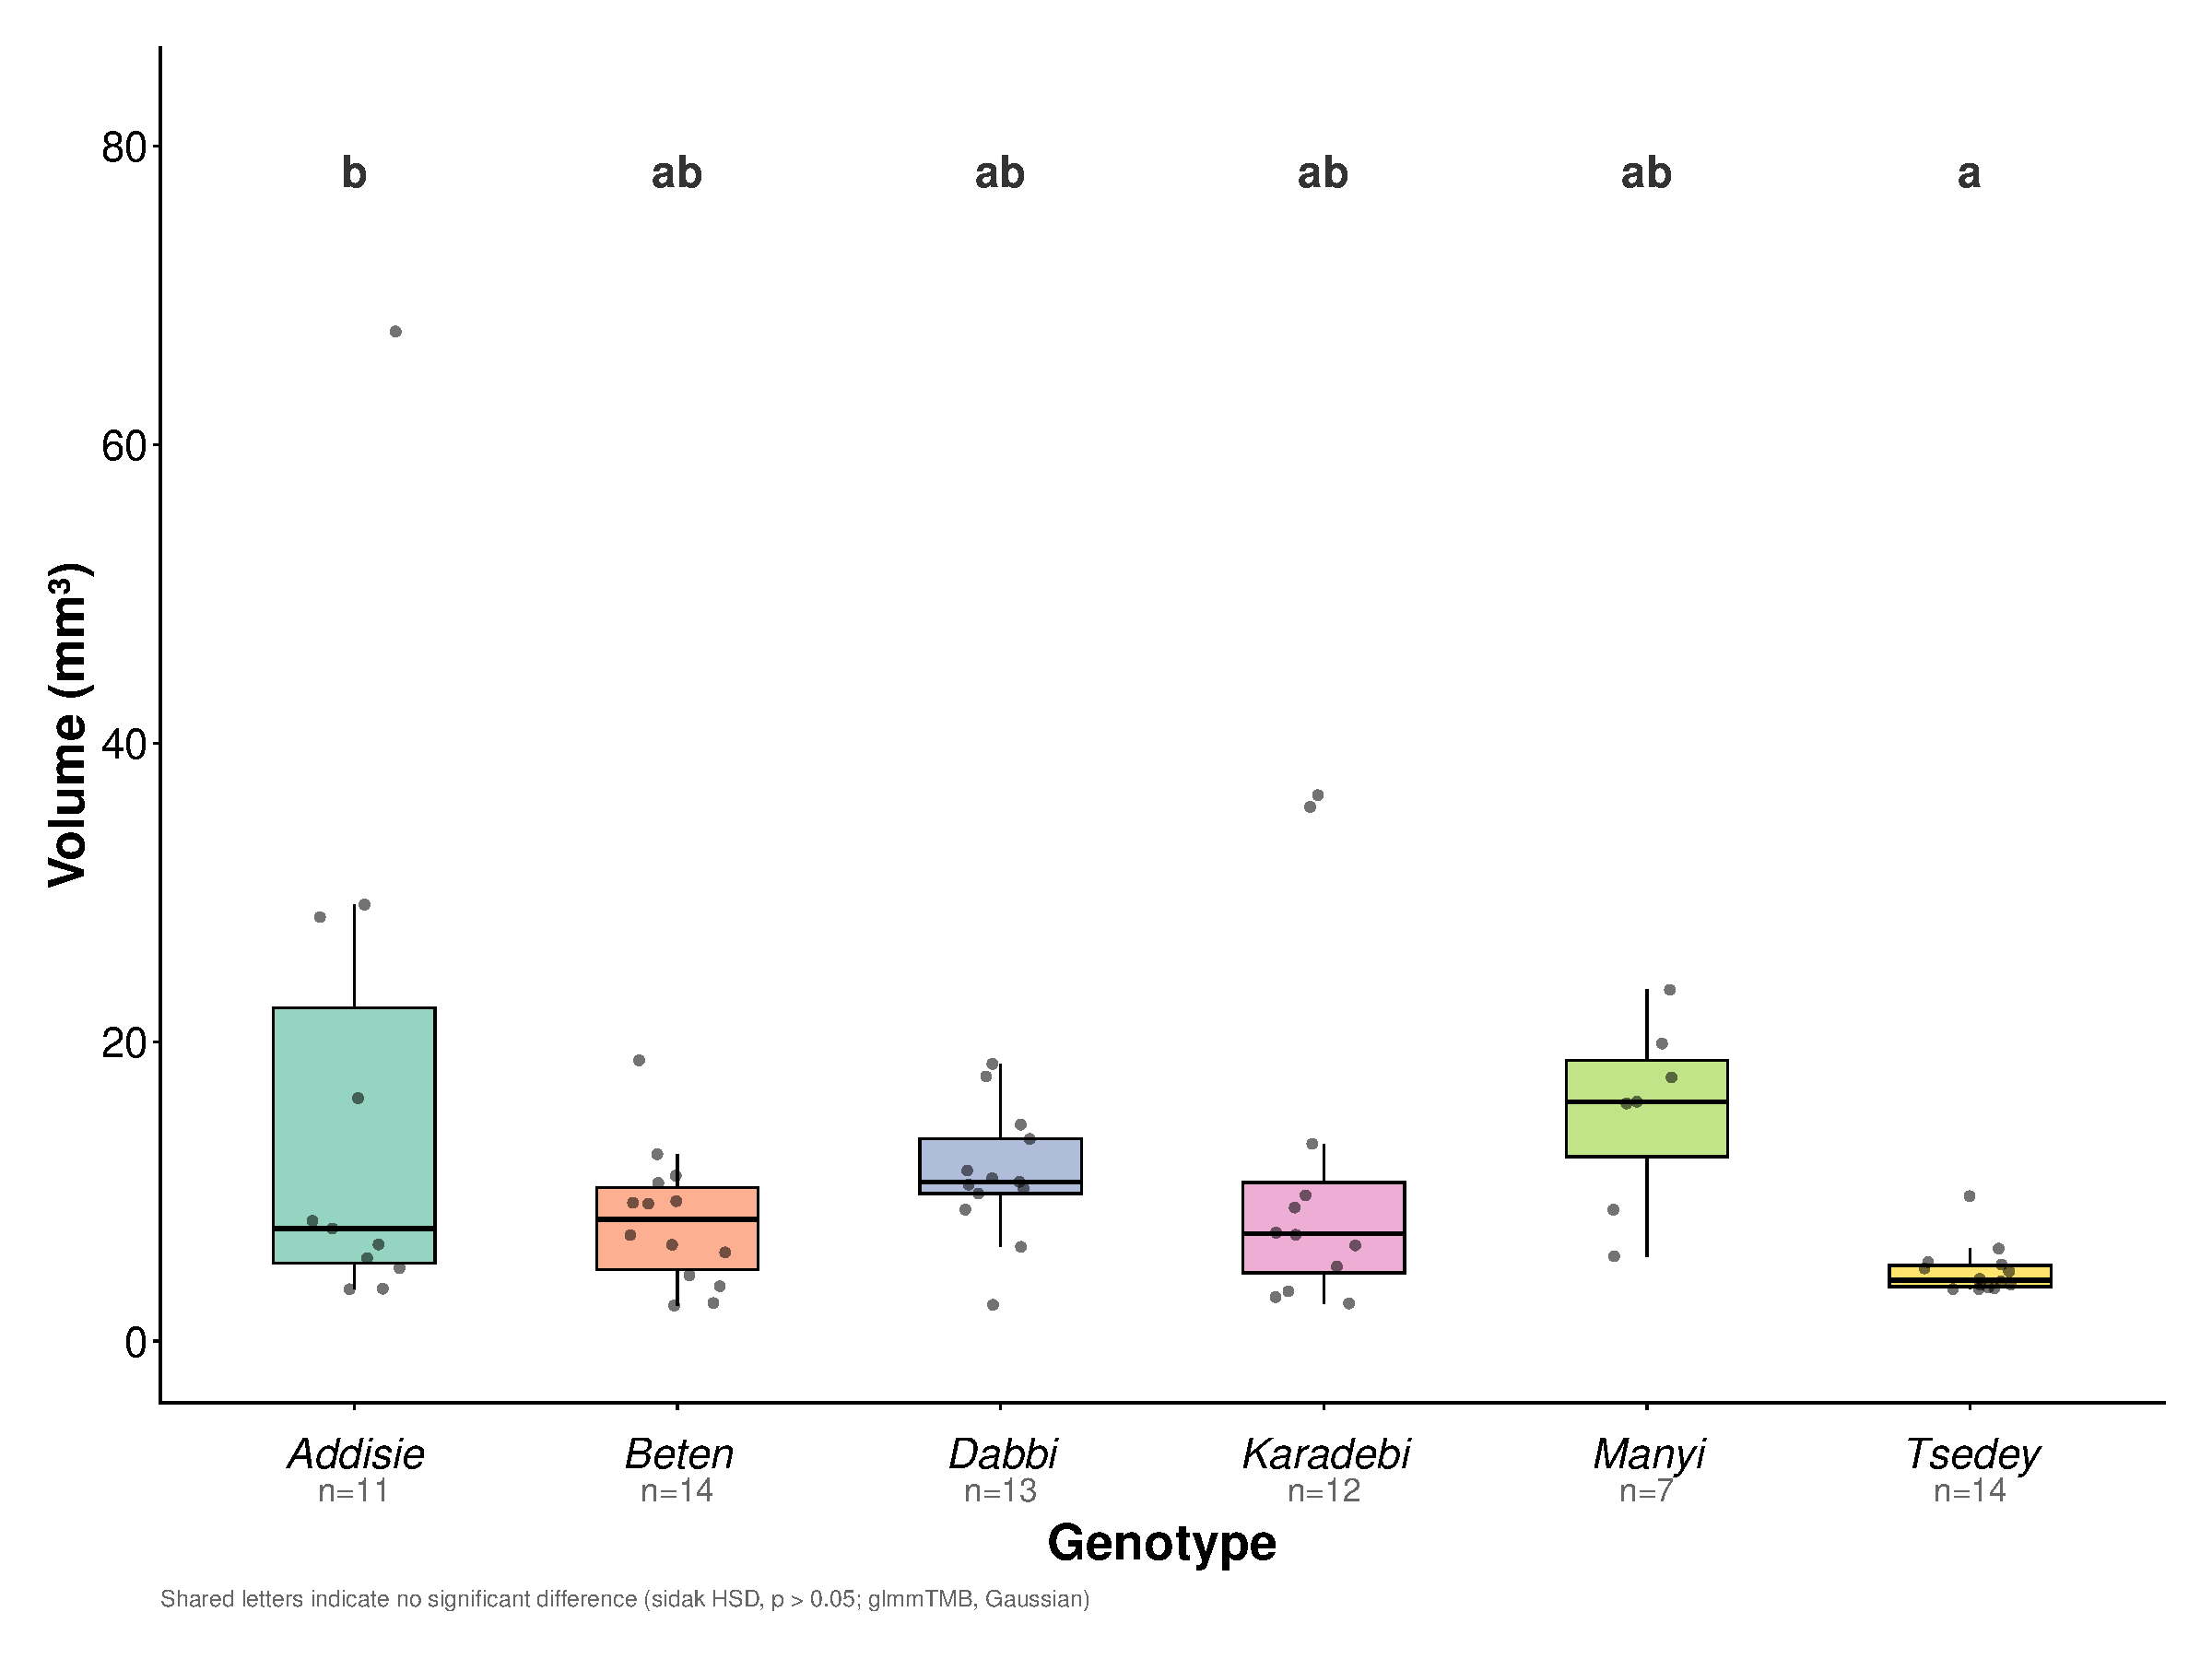
\includegraphics[keepaspectratio]{rsa_day1617_agar_files/figure-pdf/unnamed-chunk-12-14.pdf}}




\end{document}
